\documentclass[11pt,a4paper]{article}
\usepackage[margin=1in]{geometry}
\usepackage{amsmath,amssymb,bm,mathtools}
\usepackage{graphicx}
\usepackage{booktabs}
\usepackage{array,longtable}%
\usepackage{tikz}
\usepackage[compat=1.1.0]{tikz-feynman}
\usepackage[numbers,sort&compress]{natbib}
\usepackage[colorlinks=true,linkcolor=blue,citecolor=blue,urlcolor=blue]{hyperref}
\usepackage{orcidlink}
\graphicspath{{figures/}}
\allowdisplaybreaks
\numberwithin{equation}{section}%
\setlength{\parskip}{3pt}
\setlength{\emergencystretch}{2.5em}%
\makeatletter
\renewcommand*\l@subsection{\@dottedtocline{2}{1.5em}{3.0em}}%
\makeatother
\usepackage{caption}
\captionsetup[table]{position=top,skip=6pt}%

\newcommand{\MP}{M_{\mathrm{P}}}                 %
\newcommand{\MPbar}{\bar M_{\mathrm{P}}}         %
\newcommand{\Tr}{\operatorname{tr}}
\newcommand{\NC}{N_C}                            %
\newcommand{\GeV}{\,\mathrm{GeV}}
\newcommand{\MSbar}{\overline{\mathrm{MS}}}
\newcommand{\mt}{m_t}                            %
\newcommand{\mtpole}{m_t^{\mathrm{pole}}}        %
\newcommand{\mtbar}{\bar m_t}                    %
\newcommand{\mub}{\mu_b}                         %
\newcommand{\Lb}{L_b}                            %
\newcommand{\lamc}{\lambda_c}                    %
\newcommand{\xiH}{\xi_H}                         %
\newcommand{\xic}{\xi_c}                         %
\newcommand{\Pone}{P_1}                          %
\newcommand{\Pbar}{\bar P_1}                     %
\newcommand{\fzm}{f_0}                           %
\newcommand{\dLSS}{d_{\mathrm{LSS}}}             %
\newcommand{\rT}{r_{\mathrm{T}}}                 %
\newcommand{\sfloor}{\sigma_{\mathrm{floor}}}

\newcommand{\PbarOne}{0.73}        %
\newcommand{\PbarOneAbs}{0.7}      %
\newcommand{\PbarMSR}{0.50}        %
\newcommand{\PbarSigma}{0.86}      %
\newcommand{\PbarInterp}{0.68}     %
\newcommand{\PbarBKPV}{0.63\text{--}0.67} %
\newcommand{\BayesMax}{0.75}       %
\newcommand{\mExclTheory}{173.7}   %
\newcommand{\mExclFCC}{173.7}      %
\newcommand{\sigFCC}{5.3}          %
\newcommand{\sigHLLHCmin}{1.7}     %
\newcommand{\sigHLLHCmax}{2.5}     %
\newcommand{\xiHmin}{0.08}         %
\newcommand{\xiHcentral}{0.074}    %
\newcommand{\xiHhalf}{0.12}        %
\newcommand{\marginGeV}{0.36}      %
\newcommand{\marginLam}{0.0024}    %
\newcommand{\mcMinusMzero}{1.9}    %
\newcommand{\modelErrUp}{0.07}     %
\newcommand{\modelErrDn}{0.08}     %
\newcommand{\modelErrUpPnine}{0.04}     %
\newcommand{\modelErrDnPnine}{0.06}     %
\newcommand{\modelErrUpPone}{0.12}      %
\newcommand{\modelErrDnPone}{0.13}      %
\newcommand{\modelErrUpNoViPnine}{0.02} %
\newcommand{\modelErrDnNoViPnine}{0.04} %
\newcommand{\modelErrUpNoVi}{0.03}      %
\newcommand{\modelErrDnNoVi}{0.05}      %
\newcommand{\modelErrUpNoViPone}{0.04}  %
\newcommand{\modelErrDnNoViPone}{0.06}  %
\newcommand{\PbarQlo}{0.39}             %
\newcommand{\PbarQhi}{0.99}             %
\newcommand{\PbarGeHalf}{0.78}          %
\newcommand{\xiHminEW}{0.09}            %
\newcommand{\xiHbandSM}{0.013}          %
\newcommand{\xiHbandAs}{0.04}           %
\newcommand{\PbarATLASCMS}{0.76}     %
\newcommand{\PbarCMS}{0.97}          %
\newcommand{\PbarMbarSigma}{0.62}    %
\newcommand{\BselDirect}{1.59}       %
\newcommand{\BselMax}{2.18}          %
\newcommand{\mExclMeas}{174.2}       %
\newcommand{\mExclMeasInterp}{174.5} %
\newcommand{\mSurvFCC}{172.7}         %
\newcommand{\sigFCCamb}{6.0}          %
\newcommand{\sigHLLHCinterpMin}{1.1}  %
\newcommand{\sigHLLHCinterpMax}{1.2}  %
\newcommand{\lamcErrUp}{0.0006}       %
\newcommand{\lamcErrDn}{0.0005}       %
\newcommand{\PoneAtExclFCC}{0.023} %
\newcommand{\BexFCC}{0.033}        %

\providecommand{\aFitA}{5.915}%
\providecommand{\bFitA}{1.306}%
\providecommand{\resFitA}{0.06}%
\providecommand{\lamFitLo}{-0.018}%
\providecommand{\lamFitHi}{-0.007}%
\providecommand{\sigEffA}{0.44}%
\providecommand{\closedAccSmall}{1.1\%}%
\providecommand{\closedAccLarge}{3.2\%}%
\providecommand{\lcAhundred}{-0.0144}%
\providecommand{\lcAthree}{-0.0118}%
\providecommand{\lcAtenk}{-0.0072}%
\providecommand{\lcBthree}{-0.0121}%
\providecommand{\lcCthree}{-0.0124}%
\providecommand{\lcDthree}{-0.0115}%
\providecommand{\lcEthree}{-0.0128}%
\providecommand{\lamTop}{-0.028}%
\providecommand{\lcAthreeErrUp}{0.0003}%
\providecommand{\lcAthreeErrDn}{0.0002}%
\providecommand{\topGapLo}{0.3}%
\providecommand{\topGapHi}{0.9}%
\providecommand{\SwkbLo}{2}%
\providecommand{\SwkbHi}{8}%
\providecommand{\NeffHalf}{250}%
\providecommand{\NeffRatio}{0.83}%
\providecommand{\NstarA}{970}%
\providecommand{\NstarD}{590}%
\providecommand{\NstarE}{1.8\times10^5}%
\providecommand{\zpSlopeLo}{0.7}%
\providecommand{\zpSlopeHi}{1.2}%
\providecommand{\dVredLo}{12\%}%
\providecommand{\dVredHi}{32\%}%
\providecommand{\crossShiftLc}{0.0008}%
\providecommand{\SzeroGeneric}{10^{-11}}%
\providecommand{\staticHazardDiff}{0.0003\text{--}0.0004}%
\providecommand{\kappaZero}{0.48}%
\providecommand{\kappaMin}{0.43}%
\providecommand{\lcKappaThreeQ}{-0.0047}%
\providecommand{\lcKappaOne}{-0.0125}%
\providecommand{\lcKappaOneHalf}{-0.0378}%
\providecommand{\lcSthirtyGtwo}{22\%}%
\providecommand{\lcSthirtyGY}{6\%}%
\providecommand{\lcSthirtyYt}{18\%}%
\providecommand{\abelLamMin}{-1}%
\providecommand{\abelLamMax}{-0.0065}%
\providecommand{\abelSlopeLo}{1.8}%
\providecommand{\abelSlopeHi}{4.0}%
\providecommand{\abelSlopeWKB}{4.44}%
\providecommand{\abelBOdev}{30\%}%
\providecommand{\abelCAP}{10^{-6}}%
\providecommand{\abelLamcThree}{-0.091}%
\providecommand{\abelLamcSM}{-0.071}%
\providecommand{\abelHolonomy}{9\times10^{-4}}%
%

\hypersetup{pdftitle={Casimir Cosmology: Derivations and Numerical Validation},pdfauthor={Alan Zhang}}

\begin{document}

\begin{titlepage}
\begin{center}
{\LARGE\bfseries Casimir Cosmology: Derivations and Numerical Validation\par}
\vspace{1.2em}
{\large Alan Zhang\,\orcidlink{0009-0000-1187-0755}\par}
\vspace{0.5em}
{\small Department of Physics and Astronomy, McMaster University, Hamilton, Ontario L8S 4M1, Canada\\
Perimeter Institute for Theoretical Physics, Waterloo, Ontario N2L 2Y5, Canada\\
\href{mailto:zhana142@McMaster.ca}{zhana142@McMaster.ca}\par}
\vspace{1.2em}
\begin{tabular}{@{}>{\raggedright\arraybackslash}p{0.2\textwidth}>{\raggedright\arraybackslash}p{0.72\textwidth}@{}}
Report version & 1.1 (October 22, 2026); version 1.0: October 17, 2026\\
Report record & doi:\href{https://doi.org/10.5281/zenodo.23554537}{10.5281/zenodo.23554537} (this version); all versions: doi:\href{https://doi.org/10.5281/zenodo.23434139}{10.5281/zenodo.23434139} (separate from the code and data)\\
Companion Letter & A.~Zhang, \emph{Gauge Field Fluctuations Protect the Higgs Vacuum When a Small Universe Begins} (2026), \href{https://arxiv.org/abs/2610.28704}{arXiv:2610.28704}\\
Companion paper & A.~Zhang, \emph{A Casimir turning point as the beginning of a small flat universe} (2026), \href{https://arxiv.org/abs/2610.24905}{arXiv:2610.24905}\\
Code and data & doi:\href{https://doi.org/10.5281/zenodo.23434067}{10.5281/zenodo.23434067} (all versions; version 1.2.0 contains this report)\\
Status & Companion technical report; not independently peer reviewed.
\end{tabular}
\end{center}
\vspace{1em}
\begin{abstract}
This report is the companion of a Letter and a paper on a flat three-torus universe whose contraction is turned around by the negative Casimir energy of the Standard Model, with antiperiodic fermions, at an edge of $722$ reduced Planck lengths.
Part~I derives the model step by step: the trace anomaly at a turning point, the Casimir energy and the zero modes of the Standard Model on the torus, the turning solution, and the Higgs zero mode, whose negative quartic coupling, $\lambda(\mub)\approx-0.0098$, is confined by the zero-point energy of the constant gauge modes down to a finite-volume threshold $\lambda_c\approx-0.012$.
We give the finite-volume matching, the reduced two-dimensional model and its resonance, the cross terms with the non-zero modes, survival along the turn, the threshold of a static box, which depends on its duration only logarithmically and is due to the gauge zero modes, the Standard Model mapping and the top-quark criterion (survival with probability above $1/2$ for a pole mass below $172.96$~GeV, and $\bar P_1\approx\PbarOne$ for current data, given a curvature coupling $\xiH\gtrsim\xiHmin$) with its error budget.
Part~I then treats the emptiness gate, the shape of the torus and its quantum fossil, the primordial spectra and the fossil in the microwave background.
Part~II validates these results: full-dimensional diffusion Monte Carlo moves the critical mass by at most $0.031$~GeV, blind reimplementations reproduce it to $0.005$~GeV, the abelian Higgs model, whose zero-mode problem reduces exactly to two dimensions, confirms the mechanism and the WKB barrier action at the computed resonance energy, while the deep-well form of the width holds there only asymptotically, and a blind recalculation reproduces its widths to $10^{-10}$, and every computation is shown to converge; it also collects conditional evidence from a separate line of calculation and maps every number and figure to the code that produces it.
Part~III records superseded estimates and retracted statements.
\end{abstract}
\end{titlepage}

\tableofcontents
\clearpage

\section*{Reading guide}\label{rep:guide}
\addcontentsline{toc}{section}{Reading guide}

This report is the companion of a Letter~\cite{v12PRL} and a paper~\cite{v12PRD} on a flat three-torus universe whose contraction is turned around by the negative Casimir energy of the Standard Model.
The Letter computes the finite-volume threshold below which the Higgs zero mode of a small box with antiperiodic fermions keeps its vacuum with probability less than $1/2$, shows that it is due to the zero-point fluctuations of the constant gauge modes, and applies it to a universe that begins at the turning point, which gives a criterion on the top-quark mass; the paper develops the whole scenario, from the trace anomaly to the fossil of the shape in the microwave background.
Both are self-contained.
The report collects what they could not: the derivations step by step, from the definitions to the final formulas, the numerical methods, the cross-checks between different methods, the convergence of every computation, the independent reimplementations, and a guide to the code and data from which every number and figure is produced.
It is not independently peer reviewed.

\paragraph{Three parts.}
Part~I (Secs.~\ref{rep:setup}--\ref{rep:sky}) is the final model and its derivations, in the order of the physical argument: the assumptions, the trace anomaly at a turning point, the Casimir energy and zero modes of the Standard Model on the torus, the turning solution, six sections on the Higgs zero mode (finite-volume matching, the reduced model and its resonance, the cross terms with the non-zero modes, survival along the turn, the Standard Model mapping and the top-quark criterion, the error budget and the curvature coupling), the emptiness gate, the shape of the torus and its quantum fossil, the primordial spectra, and the reading of the fossil in the sky.
Part~II (Secs.~\ref{rep:v-fulldim}--\ref{rep:v-repro}) is the evidence that Part~I is computed correctly: the full-dimensional checks of the reduced zero-mode model and an exactly reducible test of the mechanism in the abelian Higgs model, the independent (blind) reimplementations, the convergence and numerical controls, the results of a separate line of calculation that we use only as conditional evidence, and the reproduction guide.
Part~III (Sec.~\ref{rep:history}) is a record of superseded estimates, failed approaches and retracted statements; nothing in it is used in the papers.
Appendix~\ref{rep:app-notation} lists the notation and Appendix~\ref{rep:app-numbers} the key numbers with their sources.

\paragraph{Reading alongside the Letter and the paper.}
Table~\ref{tab:guide-map} shows where the material of the two papers is expanded here.
The paper refers to this report as ``Ref.~\cite{v12Report}, Sec.~$N$''; the section numbers of this report are fixed.
A reader who wants the main results only can read the Letter, then Secs.~\ref{sec:v11-static-box}--\ref{sec:v11-static-torus} for the static-box threshold and Sec.~\ref{sec:v11-abelian} for the abelian test, Secs.~\ref{rep:h-smmap} and~\ref{rep:h-budget} for the criterion and its error budget, and Sec.~\ref{rep:v-blind} for how it was checked.

\begin{table}[ht]
\centering
\small
\caption{Where the material of the Letter (PRL) and of the paper (PRD) is expanded in this report.}
\label{tab:guide-map}
\begin{tabular}{@{}p{0.38\textwidth}p{0.27\textwidth}p{0.25\textwidth}@{}}
\toprule
Topic & Papers & This report \\
\midrule
Setup and assumptions A1--A8 & PRD II; PRL & Sec.~\ref{rep:setup} \\
Trace anomaly at a turning point & PRD III & Sec.~\ref{rep:trace} \\
Casimir energy, zero modes, turning solution & PRD IV and appendices & Secs.~\ref{rep:casimir}--\ref{rep:turning} \\
Higgs zero mode: matching, reduced model, cross terms & PRD V; PRL & Secs.~\ref{rep:h-matching}--\ref{rep:h-cross} \\
The confinement mechanism in field-theory context & PRL (introduction, Discussion) & Sec.~\ref{sec:v11-mechanism-context} \\
Survival along the turn, preparation, two branches & PRD V; PRL & Sec.~\ref{rep:h-survival} \\
Static box: width law, threshold $\lamc(N)$, gauge zero-mode origin, couplings & PRL (Fig.~1, End Matter A) & Sec.~\ref{sec:v11-static-box} \\
Standard Model mapping and the top-quark criterion & PRD V; PRL & Sec.~\ref{rep:h-smmap} \\
Error budget, marginalization, experimental reach & PRD V; PRL Table~I & Sec.~\ref{rep:h-budget} \\
Universality and the curvature coupling $\xiH$ & PRD V; PRL & Sec.~\ref{rep:h-universality} \\
Emptiness gate & PRD VI & Sec.~\ref{rep:gate} \\
Shape no-go, real-moment theorem, fossil & PRD VII; PRL & Secs.~\ref{rep:shape}, \ref{rep:quantum-shape} \\
Primordial spectra and the microwave-background window & PRD VIII & Secs.~\ref{rep:spectra}, \ref{rep:sky} \\
Full-dimensional validation, verification record & PRD V and appendices; PRL & Secs.~\ref{rep:v-fulldim}, \ref{rep:v-blind} \\
Abelian Higgs model: an exactly reducible test & PRL End Matter A & Secs.~\ref{sec:v11-abelian}, \ref{sec:v11-blind-abelian} \\
Convergence, numerical controls & PRD appendices & Sec.~\ref{rep:v-convergence} \\
Conditional evidence & PRD VII F, VIII B, IX & Sec.~\ref{rep:v-conditional} \\
Code, data, figures, numbers & Data Availability & Sec.~\ref{rep:v-repro}, App.~\ref{rep:app-numbers} \\
\bottomrule
\end{tabular}
\end{table}

\paragraph{Version 1.1.}
Version 1.1 adds the material on which the Letter now rests: the confinement mechanism in field-theory context (Sec.~\ref{sec:v11-mechanism-context}); the finite-volume threshold of a static box as a function of its duration, its size and the couplings, and the gauge zero-mode origin of the barrier (Sec.~\ref{sec:v11-static-box}); an exactly reducible test of the mechanism and of the width law in the abelian Higgs model (Sec.~\ref{sec:v11-abelian}), with a blind recalculation (Sec.~\ref{sec:v11-blind-abelian}); and the numerical controls of these calculations (Sec.~\ref{sec:v11-numerics}).
It corrects the identification of the measured top mass with the MSR mass, which now gives $\Pbar=\PbarMSR$ (Sec.~\ref{rep:h-smmap}; item H33 of Part~III), aligns the text with the final versions of the Letter and the paper, corrects one statement of the paper (item~\ref{ret:fornal} of Sec.~\ref{sec:v23-retracted}), and adds their arXiv numbers.
The section numbers of version~1.0 are unchanged: the new material is in new subsections at the ends of Secs.~\ref{rep:h-reduced}, \ref{rep:h-survival}, \ref{rep:v-fulldim}, \ref{rep:v-blind}, \ref{rep:v-convergence} and~\ref{rep:v-repro}, and in new items of Part~III.
Figures up to Fig.~\ref{fig:rb-hazard} and tables up to Table~\ref{tab:rb-w0} keep their numbers; the later figures and tables are renumbered.

\paragraph{Conventions.}
We state the status of every result with the same words as the papers: a result is \emph{proved} (a theorem or an identity), holds \emph{under stated conditions} (``if \ldots, then \ldots''), is \emph{found numerically} (with its precision), or is \emph{expected} without proof; a representative point is never stated as an ensemble result.
The numbers of the claim layer (marginal probabilities, exclusion thresholds, reach, conditions on $\xiH$, margins and model-error totals) are typeset through macros generated from a single source in the code package, so that the Letter, the paper and this report cannot disagree (Sec.~\ref{rep:v-repro}); other numbers carry a comment with their source in the LaTeX file.
The numbers D$nnn$ and C$nnn$ identify the derivation files and calculations of the research tree, and the code package gives their original paths.
The calculation was carried out in three stages, each followed by independent checks; results of the earlier stages that were later replaced are collected in Part~III.
All figures of the papers appear in this report, including those that the paper omits, together with schematic figures and loop diagrams drawn for this report.


\part{Final model and methods}
\newcommand{\rAone}{\mathbf{1}}                          %
\newcommand{\rANeff}{N_C^{\mathrm{eff}}}                 %
\newcommand{\rAgam}{\gamma_C}                            %
\newcommand{\rAVar}{\operatorname{Var}}
\newcommand{\rACov}{\operatorname{Cov}}
\newcommand{\rATm}{\mathcal{T}}                          %
\newcommand{\rAGain}{\mathcal{G}}                        %
\newcommand{\rAHeff}{H_{\mathrm{eff}}}                   %
\newcommand{\rAsh}{\mathrm{sh}}
\newcounter{rAassump}
\renewcommand{\therAassump}{A\arabic{rAassump}}
\newcommand{\rAassume}[1]{\refstepcounter{rAassump}\label{#1}}%
\newtheorem{rAtheorem}{Theorem}[section]
\newtheorem{rAlemma}[rAtheorem]{Lemma}
\newtheorem{rAprop}[rAtheorem]{Proposition}
\newtheorem{rAcor}[rAtheorem]{Corollary}
\newenvironment{rAproof}[1][Proof]{\par\noindent\emph{#1.}\ }{\hfill$\square$\par\medskip}

\section{Setup, conventions and assumptions}\label{rep:setup}

This chapter fixes the physical setting of the whole report.
We define the geometry of a flat homogeneous universe whose spatial sections are three-tori, separate the volume from the shape, and derive the Einstein equations and the minisuperspace action that later chapters use.
We then fix units and conventions, define the two field contents that recur, and state the eight assumptions on which our results rest.
Every later chapter refers to these assumptions by number and does not repeat them.

\subsection{The physical question and the results of this report}
\label{rA:question}

The measured Higgs and top-quark masses place the Standard Model vacuum close to the boundary between stability and metastability~\cite{Degrassi:2012ry,Buttazzo:2013uya,Bednyakov:2015sca,Andreassen:2017rzq}.
Run to high energies, the Higgs quartic coupling $\lambda$ turns negative far below the Planck scale and stays small and negative up to it, so the electroweak vacuum is metastable, with a lifetime much longer than the age of the universe~\cite{Andreassen:2017rzq}.
Whether the vacuum survives the early universe is a separate question.
During inflation the Higgs field fluctuates and feels the spacetime curvature through its non-minimal coupling $\xiH$~\cite{Espinosa:2007qp,Herranen:2014cua,Kearney:2015vba,Espinosa:2015qea,Joti:2017fwe,Markkanen:2018pdo}.
For a minimally coupled plateau inflaton survival requires $\xiH\gtrsim0.06$ at the electroweak scale~\cite{Mantziris:2020rzh}, and $\xiH\gtrsim0.1$ in $R^2$ gravity~\cite{Mantziris:2022fuu}. %
After inflation the oscillating curvature limits $\xiH$ to values below about one~\cite{Herranen:2015ima}. %
All of these bounds concern a universe that is already large and inflating.

A universe that begins small poses the question in a different form.
A contracting flat universe can turn into an expanding one only if its total energy becomes non-positive at the turning point and its stress becomes negative enough to make $\dot H$ positive (Sec.~\ref{rep:trace}).
Classical fields that violate the null energy condition by that much tend to carry ghost or gradient instabilities~\cite{Dubovsky:2005xd,Kobayashi:2016xpl}, and avoiding them takes carefully engineered higher-derivative theories~\cite{Ijjas:2016tpn}.
Quantum fields offer a source without new classical degrees of freedom: on a compact flat space the vacuum energy of untwisted massless bosons is negative and grows as $L^{-4}$ when the space shrinks~\cite{DeWitt:1979dd}.
With a positive vacuum energy this Casimir energy turns a contracting three-torus around along an exact, regular solution, found by Zel'dovich and Starobinsky~\cite{Zeldovich:1984vk} and written in closed form by Guth and Vilenkin~\cite{Guth:2025dal}.
Toroidal universes that begin small were also discussed in Refs.~\cite{Coule:1999wg,Linde:2004nz,Fornal:2026qfq}.
For the Standard Model the turning point is a few thousand Planck lengths across (Sec.~\ref{rep:turning}), and there the quartic coupling is negative.

Does a beginning at such a turning point destroy the electroweak vacuum?
On a small torus the relevant degree of freedom is the Higgs zero mode, the spatially constant mode of the Higgs field, and two effects compete.
A small compact volume catalyzes false-vacuum decay, which then proceeds through a uniform tunneling mode~\cite{Hassan:2026cmp}, as does the Schwinger effect in compact directions~\cite{Brown:2015kgj}.
A small torus also gives the gauge fields zero modes of their own; at this size their zero-point fluctuations are not a small correction, and they couple to the Higgs zero mode through the covariant derivative (Sec.~\ref{rep:zeromodes}).
The Higgs chapters of this report (Secs.~\ref{rep:h-matching}--\ref{rep:h-universality}) show that the second effect prevails down to a finite-volume threshold, and that the threshold turns the question into a criterion on the top-quark mass.

The ingredients have been studied separately.
The Casimir energy of Standard Model fields on circles and tori was computed for compactifications to lower dimensions~\cite{Arkani-Hamed:2007ryu,Fornal:2011tw}, where the violation of the null energy condition by the Casimir energy is what allows the lower-dimensional vacua with horizons to exist~\cite{Arkani-Hamed:2007ryu}.
Fornal recently proposed that our universe originated from an empty, Planck-size three-torus with periodic boundary conditions, whose positive Casimir energy drives its expansion~\cite{Fornal:2026qfq}; that scenario has no turning point and does not treat the Higgs zero mode.
Hamada and Shiu treated Wilson lines together with the high-scale Higgs vacuum in compactifications of the Standard Model on a circle and a two-torus~\cite{Hamada:2017yji}.
The constant modes of gauge fields on a small torus are the leading order of the small-volume expansion of Yang--Mills theory~\cite{Luscher:1982uv,Luscher:1982ma,Luscher:1983gm,Weisz:1986vu,vanBaal:1988va,vanBaal:2000zc}.
Constant gauge fields have been studied classically in Bianchi~I cosmologies~\cite{Darian:1996jf,Jin:2004vh}, and constant abelian backgrounds on tori acquire one-loop masses~\cite{Kirsten:1993ty,Kirsten:1993qp}.
Finite-volume tunneling between degenerate vacua can itself violate the null energy condition and produce a bounce~\cite{Alexandre:2019ygz,Ai:2024dwi}.

The trace anomaly is the second quantum ingredient of a turning point.
The trace of the stress tensor of conformal fields is fixed by the curvature in every state~\cite{Duff:1993wm}.
Anomaly-driven isotropic cosmologies~\cite{Starobinsky:1980te,Fischetti:1979ue} and the damping of anisotropy by quantum effects~\cite{Hu:1978zd,Hartle:1979uf,Hartle:1980nn} are classic.
In the quantum creation of a closed universe studied by Barvinsky and Kamenshchik, the conformal anomaly and the Casimir energy of conformal fields select the instantons and bound the cosmological constant~\cite{Barvinsky:2006uh}; that universe is isotropic and spatially closed, whereas the torus here is flat, carries the Standard Model in the AAA structure, and faces the anisotropic obstruction of Sec.~\ref{rep:trace} and the emptiness gate of Sec.~\ref{rep:gate}.
Mithani and Vilenkin wrote the Friedmann equation of a flat, isotropic Casimir torus with the trace anomaly~\cite{Mithani:2014toa}.
In their oscillating universe, with a negative cosmological constant, the negative Casimir energy balances matter with $w=-2/3$ at the inner turning point, and excited radiation lowers the Casimir coefficient; their torus has periodic fermions, a fixed cubic shape and no Higgs field.
Earlier Casimir bounces used the stress of a single scalar, in a closed static universe~\cite{Herdeiro:2005zj} or in a fluid model of a flat torus~\cite{Godlowski:2007gx}.
The usual turning-point conditions~\cite{Solomons:2001ef} do not tell whether a conformal state can turn an anisotropic universe around; Sec.~\ref{rep:trace} answers this.

A Casimir turning point also leaves something behind.
The shape of a torus is unstable under Casimir back-reaction in two dimensions and in de~Sitter space~\cite{Seriu:1995hc,Ponton:2001hq,COMPACT:2026vdj}, and the shape is the part of the geometry that can survive to the present.
If the fundamental domain is smaller than the last-scattering sphere, the cosmic microwave background (CMB) shows matched circles~\cite{Cornish:1997ab}.
Their absence requires the shortest translation of a three-torus to exceed $0.985$ times the last-scattering diameter $\dLSS\simeq27.7$\,Gpc~\cite{Vaudrevange:2012da,COMPACT:2022nsu}, and Planck likelihood searches give comparable limits~\cite{Planck:2015gmu,COMPACT:2026uzi}. %
A torus somewhat larger than the last-scattering sphere still imprints correlations that are detectable in principle~\cite{COMPACT:2023rkp,Himeno:2026lgh}.
Directional null energy controls the completeness of anisotropic flat cosmologies and bounds their net change of shape, the fossil anisotropy~\cite{Zhou:2026szo}; a Casimir turning point is a concrete quantum source for that fossil.

\paragraph{Results derived in Part~I.}
Our main result concerns the Higgs zero mode (Secs.~\ref{rep:h-matching}--\ref{rep:h-universality}).
At the turning point the zero-point fluctuations of the $W$, $Z$ and hypercharge zero modes confine the Higgs zero mode, so a negative quartic coupling is tolerated down to a finite-volume threshold.
For $\lambda<0$ the Higgs zero mode is a resonance rather than a bound state, and the probability $\Pone$ that it survives the turn along one branch falls steeply as $\lambda$ decreases.
The threshold $\lamc$ is the value of $\lambda(\mub)$ at which $\Pone=1/2$, where $\mub=1/\Lb\simeq3.4\times10^{15}$\,GeV is the matching scale set by the size of the torus at the turn. %
Numerically $\lamc=-0.0121$, with $-0.0091$ and $-0.0152$ for $\Pone=0.9$ and $0.1$. %
The Standard Model value, $\lambda(\mub)=-0.0098$ for the measured masses, lies above it. %
A finite threshold exists in every sector that turns around and keeps a Higgs zero mode among those analysed (the fully periodic torus with an SU(3) center holonomy is not), and its size depends only logarithmically on the duration of the turn (Sec.~\ref{rep:h-universality}).
The scaling law of Sec.~\ref{rep:h-universality} gives $\lamc\approx-0.01$ wherever the gauge zero modes confine the Higgs zero mode; for the spin structures PPA and PAA, which also turn around and keep the zero mode, indicative estimates shift the critical mass by $+0.08$ and $+0.02$\,GeV, and their exact thresholds need an anisotropic model. %

The steep dependence of $\lambda(\mub)$ on the top-quark pole mass $\mt$, $d\lambda(\mub)/d\mt\simeq-0.0066\,{\rm GeV}^{-1}$, comes from the same top-Yukawa running that sets the absolute-stability bound~\cite{Degrassi:2012ry,Buttazzo:2013uya,Bednyakov:2015sca}. %
It converts the threshold into a criterion (Sec.~\ref{rep:h-smmap}): $\Pone>1/2$ if and only if $\mt<172.96$\,GeV, or $\mtbar<163.16$\,GeV for the $\MSbar$ mass $\mtbar\equiv\mtbar(\mtbar)$, at $\alpha_s(M_Z)=0.1180$. %
The Standard Model theory error of this bound is $\pm0.10$\,GeV for $\mt$ and $\pm0.07$\,GeV for $\mtbar$, and $\alpha_s\pm0.0009$ moves it by $\pm0.35$\,GeV ($\pm0.25$\,GeV for $\mtbar$). %
The model error is $+\modelErrUp/-\modelErrDn$\,GeV, dominated by the scale of inflation (Sec.~\ref{rep:h-budget}). %
The criterion lies about $\mcMinusMzero$\,GeV above the line $\lambda(\mub)=0$, which with our inputs lies only $0.1$\,GeV above the absolute-stability bound, $\mt\simeq171.0$\,GeV ($171.2$--$171.5$\,GeV for the inputs of Refs.~\cite{Buttazzo:2013uya,Bednyakov:2015sca,Andreassen:2017rzq}), and far below the metastability bound, $177.7$\,GeV~\cite{Andreassen:2017rzq}. %
Marginalizing over the measured $\mt$ and $\alpha_s$ gives a survival probability $\Pbar\simeq\PbarOneAbs$, between $\PbarMSR$ and $\PbarSigma$ depending on how the measured top mass is interpreted (Sec.~\ref{rep:h-budget}).
Current data neither favor nor disfavor survival: the Bayes factors of Sec.~\ref{rep:h-budget} obey $|\ln B|\leq\BayesMax$.
Survival through the expanding branch also needs a curvature coupling $\xiH(\mub)\gtrsim\xiHmin$; at the measured $\mt$ this condition, defined with a $1\%$ tolerance, lies above the inflationary bound for the same plateau, and the conformal value $1/6$ meets both (Sec.~\ref{rep:h-universality}).
FCC-ee can test this beginning: a measured pole mass above $\mExclFCC$\,GeV would establish $\Pone<0.1$ at $95\%$ confidence; at the threshold the central $\Pone$ is $\approx\PoneAtExclFCC$ and the Bayes factor $B_{\rm ex}\approx\BexFCC$ (Sec.~\ref{rep:h-budget}). %
The companion Letter~\cite{v12PRL} computes the finite-volume threshold of a static box as a function of its duration, its size and the couplings, shows that the gauge zero modes cause it, tests the mechanism in the abelian Higgs model, and applies the resonance to a universe that begins at a Casimir turning point; the companion paper~\cite{v12PRD} gives the full argument in compressed form.

The turning point itself needs two ingredients (Secs.~\ref{rep:trace}--\ref{rep:turning}).
For conformal matter with $a/c$ inside the conformal collider bounds and other matter of non-negative trace, the trace anomaly forbids an anisotropic universe to turn around, $\dot H\leq-5S/54$ in any state, so matter with $w<1/3$, most cheaply a positive potential, must supply the negative trace. %
With trivial gauge holonomies the Standard Model supplies the negative energy only with non-periodic spin structures: with fermions antiperiodic around all three cycles its signed Casimir weight is $+25.515$, while periodic fermions give $-30$. %
The vacuum energy of the gauge and Higgs zero modes does not depend on the shape at fixed volume and is a fraction $\fzm=0.30$ of the free Casimir energy at the cube, and with a plateau inflaton the torus turns around at $\Lb=722\,\MPbar^{-1}$. %

The remaining negative energy is worth about five quanta of the lowest nonzero modes, so the universe must be nearly empty at the turn (Sec.~\ref{rep:gate}). %
A time-symmetric past with a reheating coupling exceeds this budget by at least $10^{94}$, and natural states of non-conformal fields must be prepared within about seven e-folds of the turning point. %
We therefore read the turning point as a beginning, with arrows of time pointing away from it on both sides (assumption~\ref{assump:A4}).
The budget does not select the vacuum: a photon pair within it turns around with the universe and freezes the torus into a box whose sides are in the ratio $3.0$--$11.9$ (90\% range). %

Negative Casimir energy cannot hold a shape (Sec.~\ref{rep:shape}).
Like an Epstein zeta function it is an eigenfunction of the Laplacian on the space of shapes, so a negative one has no shape minimum, and neither thermal response, nor positive zero-mode energy, nor static holonomies create one.
The unstable shape modes grow through the turn, and their correlation grows monotonically, so the shape state is real at most once (Sec.~\ref{rep:quantum-shape}).
For a real Gaussian state, if both branches keep their shape with probability of at least $90\%$ ($99\%$), that instant lies within $0.35/h$ ($0.24/h$) of the turn. %
Every state that is never real leaves, on one branch, an outgoing shape at least $36.7$ times wider in rms than the state real at the turn (Theorem~\ref{thm:rA-real}), and the two extreme never-real states that we evolved keep their shape on both branches in only $4.3\%$ and $2.7\%$ of the trajectories. %
The natural state, real at the turn and centered on the cube (assumption~\ref{assump:A8}), freezes the global shape, with the smallest spread, to $0.05\%$, that a state real at the turn allows, into a nearly rectangular box whose longest and shortest sides typically differ by $16$--$18\%$ (Sec.~\ref{rep:quantum-shape}). %
The primordial spectra are those of the plateau (Sec.~\ref{rep:spectra}).
The CMB can read the shape fossil only if the shortest cycle of the torus lies between the matched-circle bound, $0.985\,\dLSS$, and about $1.04\,\dLSS$. %
Over the predicted distribution of shapes the probability of a readable fossil peaks at $0.34$--$0.38$ as a function of the present size, which the model does not select (Sec.~\ref{rep:sky}). %
Present circle and likelihood searches allow this window.

\paragraph{New results.}
To our knowledge two results are new in kind:
(1)~the finite-volume threshold $\lamc(\mub)$, set by the zero-point fluctuations of the gauge zero modes that confine the Higgs zero mode, and the criterion on $(\mt,\alpha_s,\xiH)$ that follows from it (Secs.~\ref{rep:h-matching}--\ref{rep:h-universality});
(2)~the time localization of the instant at which the shape state is real, a conditional theorem, together with the variance bound for states that are never real and their computed survival on both branches (Sec.~\ref{rep:quantum-shape}).
The comparison below covers work available up to October 2026. %
The closest work differs from item (1) in mechanism.
Compactness speeds up the decay of a uniform mode in a scalar potential~\cite{Hassan:2026cmp}, whereas here the gauge zero modes hold the Higgs zero mode near the origin.
Arkani-Hamed \emph{et al.}~\cite{Arkani-Hamed:2007ryu} and Hamada and Shiu~\cite{Hamada:2017yji} study lower-dimensional vacua of the compactified Standard Model, in which Wilson lines are moduli; neither concerns a cosmological beginning or a criterion for the survival of the Higgs zero mode.
The inflationary bounds on $\xiH$~\cite{Herranen:2014cua,Mantziris:2020rzh,Mantziris:2022fuu} constrain a large inflating universe; here $\xiH$ acts on the zero mode while the torus expands away from the turn.
For item (2), Kiefer and Zeh showed that a real Wheeler--DeWitt wave function with low entropy at small scale factor gives an arrow of time that formally reverses at the turning point of maximal expansion of a recollapsing universe~\cite{Kiefer:1994gp}, and Boyle, Finn and Turok proposed a universe that is CPT symmetric about a singular bang~\cite{Boyle:2018tzc}.
Our reflection surface is the regular Casimir minimum, from which the arrows point away; the statement concerns the reality of the shape state, and it comes with a quantitative bound.
The other results listed above are also derived here, several of them in more general form than in earlier work, which we cite where each enters: the obstruction of Sec.~\ref{rep:trace}, the Standard Model Casimir weights and shape Hessian for non-periodic spin structures (Sec.~\ref{rep:casimir}), the quantized emptiness bound (Sec.~\ref{rep:gate}), the extension of the shape no-go to thermal states, zero modes and holonomies (Sec.~\ref{rep:shape}), and the closed-form floor and the fossil (Sec.~\ref{rep:quantum-shape}).

\subsection{Geometry: volume, shape and the Bianchi~I equations}
\label{rA:geometry}

We consider flat homogeneous cosmologies
\begin{equation}
ds^2=-dt^2+h_{ij}(t)\,dx^idx^j ,
\label{eq:rA-metric}
\end{equation}
with comoving coordinates $x^i$ and a spatial metric $h_{ij}(t)$ that depends on time only.
The extrinsic curvature of the slices of constant $t$ is $K_{ij}=\tfrac12\dot h_{ij}$, and its mixed form $\mathsf K^i{}_j=h^{ik}K_{kj}=\tfrac12(h^{-1}\dot h)^i{}_j$ is the expansion tensor of the comoving observers.
We split it into its trace and its trace-free part,
\begin{equation}
\mathsf K=H\,\rAone+\sigma,\qquad H=\tfrac13\Tr\mathsf K=\tfrac16\,\frac{d}{dt}\ln\det h,\qquad \Tr\sigma=0,
\label{eq:rA-Ksplit}
\end{equation}
so that $H$ is the mean Hubble rate and $\sigma$ the shear, and we write $S=\Tr\sigma^2$ for the shear scalar.
In an orthonormal frame the shear is a symmetric trace-free $3\times3$ matrix.

\paragraph{Volume and shape.}
On a three-torus we choose coordinates of unit period, $x^i\sim x^i+1$, and write
\begin{equation}
h_{ij}=L^2G_{ij},\qquad \det G=1 .
\label{eq:rA-LG}
\end{equation}
Then $L^3=\sqrt{\det h}$ is the physical volume, and the five independent components of the unimodular symmetric matrix $G$ are the shape of the fundamental domain.
Inserting Eq.~\eqref{eq:rA-LG} into $\mathsf K=\tfrac12h^{-1}\dot h$ gives
\begin{equation}
\mathsf K=\frac{\dot L}{L}\,\rAone+\tfrac12\,G^{-1}\dot G .
\label{eq:rA-Kshape}
\end{equation}
Since $\Tr(G^{-1}\dot G)=d\ln\det G/dt=0$, the second term is trace free, so the volume carries the whole mean expansion, $H=\dot L/L$, and the shape carries the whole shear,
\begin{equation}
\sigma=\tfrac12\,G^{-1}\dot G,\qquad S=\tfrac14\Tr\big(G^{-1}\dot G\big)^2 .
\label{eq:rA-shear}
\end{equation}
Both statements are exact.

A change of lattice basis, $x\to Ax$ with $A\in GL(3,\mathbb Z)$, maps $G$ to $A^{\mathsf T}GA$ and describes the same torus.
These maps act on $G$ discretely, so a continuous change of $G$ is a physical change of shape, and the space of shapes is the orbifold $SL(3,\mathbb Z)\backslash SL(3,\mathbb R)/SO(3)$.
The large diffeomorphisms of the cube form its point group, the cubic group $O_h$, which permutes and reflects the three edges.

\paragraph{Shape metric and coordinates.}
On the five-dimensional space of unimodular metrics we use the physical shape metric
\begin{equation}
ds^2_{\rAsh}=\tfrac14\Tr\big(G^{-1}dG\big)^2 .
\label{eq:rA-shapemetric}
\end{equation}
It is invariant under $G\to A^{\mathsf T}GA$ for every $A\in SL(3,\mathbb R)$, and by Eq.~\eqref{eq:rA-shear} the shear scalar is the squared speed of the shape in this metric, $S=(ds_{\rAsh}/dt)^2$.
We parametrize shapes near the cube by
\begin{equation}
G=\exp\Big(2\sum_A\beta_AX_A\Big),\qquad \Tr X_AX_B=\delta_{AB},
\label{eq:rA-betaparam}
\end{equation}
with five symmetric trace-free matrices $X_A$.
Along a straight line $\beta_A(t)=\beta_A^{(0)}+v_At$ through the origin the matrices commute, $G^{-1}\dot G=2\sum_Av_AX_A$, and $ds^2_{\rAsh}=\sum_A d\beta_A^2$; the curves $t\mapsto e^{2tX_A}$ are unit-speed geodesics through the cube, and $S=\sum_A\dot\beta_A^2+\mathcal O(\beta^2\dot\beta^2)$ in general.
About the cube the five directions decompose under the cubic group into two irreducible representations.
The two aspect directions
\begin{equation}
X_d=\frac{1}{\sqrt2}\,{\rm diag}(1,-1,0),\qquad X_{d2}=\frac{1}{\sqrt6}\,{\rm diag}(1,1,-2)
\label{eq:rA-XE}
\end{equation}
span the two-dimensional representation $E$, and the three angle directions $X_{ij}=(E_{ij}+E_{ji})/\sqrt2$, $i<j$, with $E_{ij}$ the matrix units, span the three-dimensional representation $T_2$.

For small amplitudes the coordinates have a direct geometric meaning.
Along $X_d$ alone $G={\rm diag}(e^{\sqrt2\beta_d},e^{-\sqrt2\beta_d},1)$, so the edge lengths $L_i=L\sqrt{G_{ii}}$ obey
\begin{equation}
\ln\frac{L_1}{L_2}=\tfrac12\ln\frac{G_{11}}{G_{22}}=\tfrac12\big[\sqrt2\beta_d-(-\sqrt2\beta_d)\big]=\sqrt2\,\beta_d .
\label{eq:rA-aspect}
\end{equation}
Along $X_{12}$ to first order $G_{12}=\sqrt2\,\beta_{12}$ and $G_{11}=G_{22}=1$, so the cosine of the angle between the first two edges is $G_{12}/\sqrt{G_{11}G_{22}}=\sqrt2\,\beta_{12}$, and that angle is $\pi/2-\sqrt2\,\beta_{12}$.
Figure~\ref{fig:rA-shapes} sketches both kinds of deformation.

\begin{figure}[tbp]
\centering
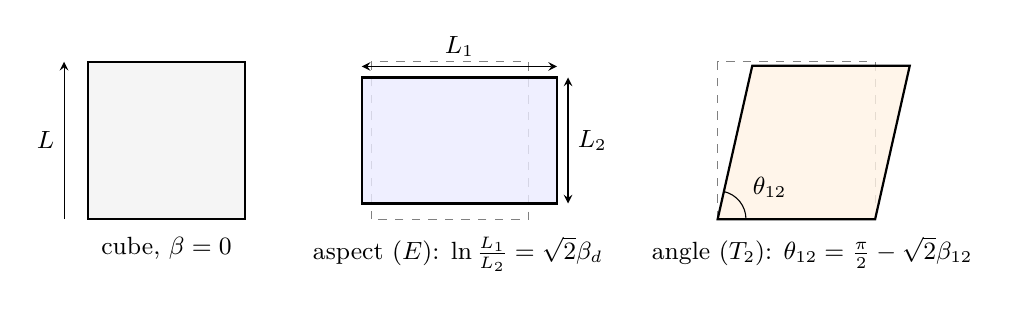
\begin{tikzpicture}[scale=2.0,>=stealth]
  \draw[thick,fill=gray!8] (0,0) rectangle (1,1);
  \node[below] at (0.5,-0.05) {\small cube, $\beta=0$};
  \draw[->] (-0.15,0) -- (-0.15,1) node[midway,left] {\small $L$};
  \begin{scope}[xshift=1.8cm]
    \draw[dashed,gray] (0,0) rectangle (1,1);
    \draw[thick,fill=blue!8,fill opacity=0.8] (-0.06,0.1) rectangle (1.18,0.9);
    \node[below] at (0.55,-0.05) {\small aspect ($E$): $\ln\frac{L_1}{L_2}=\sqrt2\beta_d$};
    \draw[<->] (-0.06,0.97) -- (1.18,0.97) node[midway,above] {\small $L_1$};
    \draw[<->] (1.25,0.1) -- (1.25,0.9) node[midway,right] {\small $L_2$};
  \end{scope}
  \begin{scope}[xshift=4.0cm]
    \draw[dashed,gray] (0,0) rectangle (1,1);
    \draw[thick,fill=orange!10,fill opacity=0.8] (0,0) -- (1,0) -- (1.22,0.975) -- (0.22,0.975) -- cycle;
    \draw (0.18,0) arc (0:77:0.18);
    \node at (0.33,0.2) {\small $\theta_{12}$};
    \node[below] at (0.6,-0.05) {\small angle ($T_2$): $\theta_{12}=\frac\pi2-\sqrt2\beta_{12}$};
  \end{scope}
\end{tikzpicture}
\caption{Shape coordinates of the torus, shown on one face of the fundamental domain at fixed volume.
Left: the cube.
Middle: an aspect deformation along $X_d$, one of the two directions of the representation $E$ of the cubic group; the second, $X_{d2}$, lengthens two edges and shortens the third.
Right: an angle deformation along $X_{12}$, one of the three directions of $T_2$.
Both deformations are drawn far larger than the quantum fossil of Sec.~\ref{rep:quantum-shape}, whose aspect amplitudes are of order $0.1$ and whose angle amplitudes are of order $0.007$.}
\label{fig:rA-shapes}
\end{figure}

\paragraph{Einstein equations.}
For Eq.~\eqref{eq:rA-metric} the flat slices have vanishing intrinsic curvature, and the Gauss--Codazzi relations give the spacetime curvature entirely through $\mathsf K$ (Sec.~\ref{rep:trace}).
The Hamiltonian constraint, $R^{(3)}+\tfrac23\theta^2-\sigma_{ab}\sigma^{ab}=2\rho/\MPbar^2$ with expansion $\theta=3H$ and $R^{(3)}=0$, reads $6H^2-S=2\rho/\MPbar^2$, and Raychaudhuri's equation for the geodesic comoving observers reads $\dot\theta=-\tfrac13\theta^2-S-(\rho+3\bar p)/2\MPbar^2$.
Together
\begin{equation}
3\MPbar^2H^2=\rho+\tfrac12\MPbar^2S,\qquad
\dot H=-\frac{\rho+\bar p}{2\MPbar^2}-\tfrac12S ,
\label{eq:rA-einstein}
\end{equation}
where $\rho$ is the energy density and $\bar p=\tfrac13\Tr p$ the mean pressure; the second equation follows from Raychaudhuri's after eliminating $3H^2$ with the constraint.
The trace-free part of the spatial equations is the shape equation, which the minisuperspace action below gives in a more useful form.

\paragraph{Minisuperspace action.}
Per unit coordinate volume and with unit lapse, the Einstein--Hilbert action of Eq.~\eqref{eq:rA-metric} reduces to $\tfrac12\MPbar^2\sqrt h\,(K_{ij}K^{ij}-K^2)$, with $K_{ij}K^{ij}=\Tr\mathsf K^2=3H^2+S$ and $K=3H$.
Adding matter with energy $E(L,G)=L^3\rho$ gives
\begin{equation}
\mathcal L=-3\MPbar^2L\dot L^2+\tfrac12\MPbar^2L^3\,\tfrac14\Tr\big(G^{-1}\dot G\big)^2-E(L,G),
\label{eq:rA-minisuperspace}
\end{equation}
so the volume has a negative kinetic term and the shape is a sigma model on the space of unimodular metrics, with the metric of Eq.~\eqref{eq:rA-shapemetric} and the inertia $\MPbar^2L^3$.
Variation of the lapse gives the constraint of Eq.~\eqref{eq:rA-einstein}.
Near the cube the shape momenta are
\begin{equation}
P_A=\MPbar^2L^3\dot\beta_A ,
\label{eq:rA-PA}
\end{equation}
and the shape equations are $d(\MPbar^2L^3\dot\beta_A)/dt=-\partial E/\partial\beta_A$ to linear order in $\beta$.
Sections~\ref{rep:gate}, \ref{rep:shape} and~\ref{rep:quantum-shape} use these equations with the Casimir energy as $E$.

\subsection{Units and conventions}
\label{rA:units}

Units are $\hbar=c=1$, and $\MPbar=(8\pi G)^{-1/2}=2.435\times10^{18}$\,GeV is the reduced Planck mass; we never use the non-reduced Planck mass. %
The Planck length is $\ell_{\rm P}=G^{1/2}=1/(\sqrt{8\pi}\,\MPbar)$.
The signature is $(-,+,+,+)$, and the trace of the stress tensor is $T=-\rho+3\bar p$.
We measure time $t$ from the turning point and write $\tau\equiv ht$, where $h$ is the plateau scale of assumption~\ref{assump:A3}; the true rate of the turning-point solution, $\rAHeff=0.98949\,h$, is introduced in Sec.~\ref{rep:turning}. %
In Sec.~\ref{rep:trace} the symbols $a$ and $c$ are anomaly coefficients; elsewhere $a$ is a scale factor.
The couplings $\lambda$, $g_3$, $g_2$, $g_Y$ and $y_t$ are running $\MSbar$ couplings, with $g_Y$ the hypercharge coupling in the Standard Model normalization and the Higgs potential written as $\lambda(\Phi^\dagger\Phi-v^2/2)^2$; unless we say otherwise they are evaluated at the matching scale $\mub$ of assumption~\ref{assump:A2}.
The non-minimal coupling enters the action as $-\xiH R\,\Phi^\dagger\Phi$, so that the conformal value is $\xiH=1/6$.
Quantities in units of $1/L$ are energies of the torus at fixed volume; conformal time $\eta$ is defined by $dt=L\,d\eta$, so that a light ray crosses the torus once per unit of $\eta$.
Notation is collected in Appendix~\ref{rep:app-notation} and the key numbers, with their source files and keys, in Appendix~\ref{rep:app-numbers}.

\subsection{Field contents}
\label{rA:content}

Two field contents recur.
The \emph{Standard Model} content is its high-energy field content, the twelve gauge vectors, the Higgs doublet and 45 Weyl fermions (no right-handed neutrinos), together with the static graviton, whose two polarizations count as one Maxwell field in the Casimir energy. %
In units of the Casimir energy of one Maxwell field, which has two physical polarizations, the bosons count $B=12+2+1=15$: twelve vectors, the four real Higgs components (two units) and the graviton.
The fermions count $F=45$, one unit per Weyl fermion.
The \emph{Maxwell toy} consists of $N_v$ periodic Maxwell fields plus the static graviton; it is a controlled model for which we also compute the causal response and the nonlinear evolution of the shape (Secs.~\ref{rep:shape} and~\ref{rep:quantum-shape}).

\subsection{Assumptions}
\label{rA:assumptions}

Our results rest on eight assumptions, which we state here once.
\begin{itemize}
\item[(A1)]\rAassume{assump:A1}
Einstein gravity sourced by the expectation value of the stress tensor, $\MPbar^2G_{\mu\nu}=\langle T_{\mu\nu}\rangle$, for homogeneous expectation values~\cite{Hartle:1981zt}, with the volume and the inflaton treated classically, except where Secs.~\ref{rep:quantum-shape} and~\ref{rep:sky} quantize the volume and the inflaton zero mode to test the reality condition, the shear criterion and the spread of sizes, and with the shape moduli and the zero modes treated quantum mechanically.
Space is a flat three-torus; the fermions are antiperiodic around all three cycles (the AAA spin structure), the gauge holonomies are trivial, and there is no 't~Hooft flux.
\item[(A2)]\rAassume{assump:A2}
The Standard Model, with a non-minimal coupling $\xiH R\,\Phi^\dagger\Phi$ of the Higgs doublet to the Ricci scalar, holds up to the scale $2\pi\mub$ of the lowest non-zero modes, where $\mub\equiv1/\Lb=\MPbar/722\simeq3.4\times10^{15}$\,GeV is the matching scale. %
Its $\MSbar$ couplings at $\mub$ follow from next-to-next-to-leading-order (NNLO) matching at the top-quark mass and three-loop running, with $M_h=125.13$\,GeV and $\alpha_s(M_Z)=0.1180$~\cite{ParticleDataGroup:2026mpi} (Sec.~\ref{rep:h-smmap}). %
New states below $\mub$ that couple to the Higgs would change $\lambda(\mub)$: Yukawa couplings of heavy right-handed neutrinos lower it~\cite{Casas:1999cd,Rodejohann:2012px} and would move the criterion of Sec.~\ref{rep:h-smmap} to smaller $\mt$, whereas extra scalars can raise it; the criterion tests the Standard Model up to $2\pi\mub$.
Heavier states that couple to the Higgs field would generate a term $c\,\phi^6/M^2$ with $M<\MPbar$, and the criterion assumes that such states, if present, lie near $\MPbar$ or couple weakly to the Higgs field (Sec.~\ref{sec:v11-mechanism-context}).
\item[(A3)]\rAassume{assump:A3}
An inflaton with a plateau potential supplies the negative trace at the turning point (Sec.~\ref{rep:trace}) and the inflation that follows.
Our benchmark member of this family is
\begin{equation}
V(\phi)=3\MPbar^2h^2\big(1-e^{-\sqrt{2/3}\,\phi/\MPbar}\big)^2,
\label{eq:rA-plateau}
\end{equation}
the Einstein-frame potential of Starobinsky's model~\cite{Starobinsky:1980te} for a minimally coupled scalar, with $h$ fixed by the observed scalar amplitude (Sec.~\ref{rep:turning}), and the error budget of Sec.~\ref{rep:h-budget} varies the inflation scale over the family.
The inflaton enters the Higgs results only through $\mub$ and the duration of the turn: we assume no direct inflaton--Higgs coupling (portal or mixed non-minimal terms).
\item[(A4)]\rAassume{assump:A4}
The turning point is a beginning: each of the two branches, the contracting one before the turn and the expanding one after it, is read with its arrow of time pointing away from the turn (Sec.~\ref{rep:gate}).
$\Pone$ is the survival probability of the Higgs zero mode along one branch, conditional on its being in the finite-volume resonance at the turn.
The preparation weight of that resonance, $w_0=0.98$--$0.995$, follows from the rule of assumption~\ref{assump:A8}, the time-symmetric Gaussian of minimal energy variance (Sec.~\ref{rA:s-equivalent}), applied to the Higgs zero mode (Sec.~\ref{rep:h-survival}). %
\item[(A5)]\rAassume{assump:A5}
The dynamics of the Higgs zero mode is computed in the reduced model of Sec.~\ref{rep:h-reduced}, whose errors, including a full-dimensional check (Sec.~\ref{rep:v-fulldim}), are collected in the error budget of Sec.~\ref{rep:h-budget}.
\item[(A6)]\rAassume{assump:A6}
$\xiH$ is defined at $\mub$: it is the coefficient of $R\,\Phi^\dagger\Phi$ in the zero-mode Hamiltonian at the turn, and its electroweak-scale image follows from its running (Sec.~\ref{rep:h-universality}).
\item[(A7)]\rAassume{assump:A7}
$\mt$ denotes the top-quark pole mass, obtained from the $\MSbar$ mass with the pole--$\MSbar$ relation truncated at four loops, and $\mtbar\equiv\mtbar(\mtbar)$ is the $\MSbar$ mass.
We identify the direct (Monte Carlo) mass, $172.60\pm0.27$\,GeV~\cite{ParticleDataGroup:2026mpi}, with $\mt$ up to an interpretation uncertainty of about $0.5$\,GeV~\cite{Hoang:2020iah}, and use the MSR mass as a variant (Sec.~\ref{rep:h-smmap}). %
\item[(A8)]\rAassume{assump:A8}
At the turn the shape moduli are in the natural state: the time-symmetric Gaussian of minimal energy variance, centered on the cube (Secs.~\ref{rA:s-floor} and~\ref{rA:s-equivalent}), whose outgoing variance lies $0.05\%$ above the floor of Sec.~\ref{rA:s-floor}. %
The fossil and sky predictions of Secs.~\ref{rA:s-fossil} and~\ref{rep:sky} refer to this state; Sec.~\ref{rep:quantum-shape} also treats other states.
\end{itemize}
Section~\ref{rep:trace} needs only \ref{assump:A1} and the hypotheses stated with its obstruction, Secs.~\ref{rep:casimir}--\ref{rep:turning} add \ref{assump:A2} and \ref{assump:A3}, \ref{assump:A4}--\ref{assump:A7} enter from Sec.~\ref{rep:h-matching} on, and \ref{assump:A8} enters in Secs.~\ref{rep:quantum-shape} and~\ref{rep:sky}.
The emptiness gate of Sec.~\ref{rep:gate} motivates \ref{assump:A4}; the gate allows the vacuum states that \ref{assump:A4} and \ref{assump:A8} specify but does not enforce them.
Later chapters refer to these assumptions by number and do not repeat them.

\subsection{Scope of the free-field description}
\label{rA:scope}

Within this setup the Casimir energy is that of the nonzero modes of free massless fields with flat twists; their interactions enter through the one-loop finite-volume potential of the zero modes (Sec.~\ref{rep:zeromodes} and Sec.~\ref{rep:h-matching}).
All Standard Model masses are negligible at the turn, where $1/\Lb$ exceeds the electroweak scale by thirteen orders of magnitude, $\mub/v=3.37\times10^{15}/246\simeq1.4\times10^{13}$. %
Perturbative interactions of the nonzero modes correct the Casimir weights by a relative amount of order $g^2/16\pi^2$ (Sec.~\ref{rep:casimir}).
The shape moduli are treated as collective coordinates of the geometry, with the Casimir energy as their potential; the response of the fields to a moving shape is a correction of relative order $10^{-6}$ (Sec.~\ref{rep:shape}).

\subsection{Status of results and numbers}
\label{rA:status}

We label every result by the kind of evidence behind it.
A result is \emph{proved} when it follows from the stated equations by an argument given in full, \emph{conditional} when it holds under a stated hypothesis of the model or of the setting, \emph{numerically tested} when it rests on computations with documented convergence and independent checks, and \emph{open} otherwise.
Theorems and propositions are proved statements within the stated model; survival thresholds and probabilities are numerical.
Numbers that enter the claims of the companion papers are typeset with the macros of the shared files \texttt{numbers.tex} and, for the static box and the abelian Higgs model, \texttt{numbers\_c170.tex}; every other number carries, at the end of its source line, a tag \texttt{\%~[num:...]} that names its entry in the number inventories or its source file and key.
Superseded values and abandoned approaches are collected in Part~III (Sec.~\ref{rep:history}) and are not used in Part~I.

\section{The trace anomaly at a turning point}\label{rep:trace}

A contracting flat universe turns around only if, at the instant $H=0$, its total energy is non-positive and its trace is sufficiently negative.
We show that the trace anomaly forbids conformal matter alone to meet the second condition when the universe is anisotropic.
At every anisotropic zero of $H$, $\dot H\leq-5S/54$ in any state of a conformal field theory inside the conformal collider bounds, Eq.~\eqref{eq:rA-rate}. %
A turning point therefore needs matter with equation of state $w<1/3$, and a positive potential supplies the missing trace most cheaply.
The chapter derives the curvature invariants of Bianchi~I from scratch (Sec.~\ref{rA:curvature}), completes the square that the anomaly forms at a turning point (Sec.~\ref{rA:square}), proves the obstruction and the rate bound (Sec.~\ref{rA:obstruction}), excludes degenerate crossings (Sec.~\ref{rA:hidentity}) and computes what other matter must supply (Sec.~\ref{rA:supply}).
Only assumption~\ref{assump:A1} and the hypotheses stated with each result are used.

\subsection{Kinematics of a turning point}
\label{rA:kinematics}

Einstein's equations for the homogeneous metric~\eqref{eq:rA-metric}, derived in Sec.~\ref{rA:geometry}, are
\begin{equation}
3\MPbar^2H^2=\rho+\tfrac12\MPbar^2S,\qquad \dot H=-\frac{\rho+\bar p}{2\MPbar^2}-\tfrac12S .
\label{eq:rA-tr-einstein}
\end{equation}
At a turning point $H=0$.
The constraint then fixes the energy density, $\rho=-\tfrac12\MPbar^2S$, and inserting $S=-2\rho/\MPbar^2$ into the second equation gives
\begin{equation}
\dot H\big|_{H=0}=-\frac{\rho+\bar p}{2\MPbar^2}+\frac{\rho}{\MPbar^2}=\frac{\rho-\bar p}{2\MPbar^2}.
\label{eq:rA-hdot-turn}
\end{equation}
A bounce, $\dot H>0$, therefore requires $\bar p<\rho$.
With $T=-\rho+3\bar p$ the inequality $\bar p<\rho$ is equivalent to $T<-\rho+3\rho=2\rho=-\MPbar^2S$, so that~\cite{Solomons:2001ef}
\begin{equation}
\bar p<\rho=-\tfrac12\MPbar^2S\leq0\quad\Longleftrightarrow\quad T<-\MPbar^2S .
\label{eq:rA-trace-criterion}
\end{equation}
The total energy must be non-positive and the trace sufficiently negative.

The first condition has a counterpart in the null geometry of Bianchi~I.
For a null geodesic with frequency $\omega_p$ measured by the comoving observers, the optical tensor of the congruence, the expansion and shear of its transverse cross section, is the projection of $\omega_p\mathsf K$ onto the screen.
At an isotropic turning point the optical tensor of every null congruence therefore vanishes, $B_p=\omega_pH\,\rAone_2=0$.
In the language of Ref.~\cite{Zhou:2026szo}, every null direction is then saturated at that instant, and Lemma~5.1 of that reference states that the total energy at a saturated instant is non-positive.
Equation~\eqref{eq:rA-trace-criterion} adds the trace condition that a dynamical turn needs.
The rest of this chapter asks who can pay for the trace.

\subsection{Curvature invariants of Bianchi~I}
\label{rA:curvature}

The trace of conformal matter depends on the Weyl tensor and the Euler density, so we first compute both for the metric~\eqref{eq:rA-metric} without assuming a diagonal $\mathsf K$ or commuting shear.
Let $K_{ij}=\tfrac12\dot h_{ij}$, $\mathsf K^i{}_j=h^{ik}K_{kj}$ and $\mathcal V=(\det h)^{1/2}$.

\paragraph{Gauss--Codazzi.}
The slices are flat and $K_{ij}$ depends on $t$ only, so the Gauss and Codazzi relations give
\begin{equation}
R_{ijkl}=K_{ik}K_{jl}-K_{il}K_{jk},\qquad R_{0ijk}=0,\qquad R_{0i0j}=-\big(\dot K_{ij}-K_{ik}\mathsf K^k{}_j\big).
\label{eq:rA-gauss}
\end{equation}
The last relation follows from the geodesic deviation of the comoving observers: the separation vector $\xi$ obeys $\nabla_u\xi=\mathsf K\xi$, and the second derivative gives the tidal matrix $R^i{}_{0j0}=-(\dot{\mathsf K}+\mathsf K^2)^i{}_j$.
Lowering the index with $h_{ij}$ and using $h_{ik}\dot{\mathsf K}^k{}_j=\dot K_{ij}-2K_{ik}\mathsf K^k{}_j$ gives the form quoted.

\paragraph{Frame components.}
We now use an orthonormal frame transported along the comoving geodesics.
Because $\Gamma^i_{tk}=\mathsf K^i{}_k$, the covariant time derivative of the mixed tensor $\mathsf K$ equals its ordinary derivative, $(\nabla_t\mathsf K)^i{}_j=\dot{\mathsf K}^i{}_j$, so the frame components of $\mathsf K$ obey the same equations as the mixed components.
We write
\begin{equation}
\mathsf K=H\rAone+\sigma,\qquad u\equiv\dot\sigma,\qquad P\equiv\sigma^2-\tfrac13S\,\rAone ,
\label{eq:rA-uP}
\end{equation}
where $\sigma$ and $u$ are symmetric and trace free but need not commute.
The characteristic polynomial of a trace-free $3\times3$ matrix gives $\sigma^3=\tfrac12S\,\sigma+(\det\sigma)\rAone$, hence $\Tr\sigma^3=3\det\sigma$ and
\begin{equation}
\Tr\sigma^4=\tfrac12S^2,\qquad \Tr P^2=\Tr\sigma^4-\tfrac23S^2+\tfrac13S^2=\tfrac16S^2,\qquad \Tr(\sigma P)=\Tr\sigma^3 .
\label{eq:rA-cayley}
\end{equation}

\paragraph{Ricci tensor.}
In the frame, Eq.~\eqref{eq:rA-gauss} gives $R_{0i0j}=-(\dot{\mathsf K}+\mathsf K^2)_{ij}$ and $R^k{}_{ikj}=(\Tr\mathsf K)\,\mathsf K_{ij}-(\mathsf K^2)_{ij}$.
Hence
\begin{equation}
\begin{aligned}
R_{00}&=-\Tr\big(\dot{\mathsf K}+\mathsf K^2\big)=-\big(3\dot H+3H^2+S\big),\\
R_{ij}&=\big(\dot{\mathsf K}+(\Tr\mathsf K)\mathsf K\big)_{ij}=\big(\dot H+3H^2\big)\delta_{ij}+u_{ij}+3H\sigma_{ij},\\
R&=-R_{00}+\Tr R_{ij}=6\dot H+12H^2+S .
\end{aligned}
\label{eq:rA-ricci}
\end{equation}
With $R_{00}=(\rho+3\bar p)/2\MPbar^2$ the first line is Raychaudhuri's equation used in Eq.~\eqref{eq:rA-einstein}.

\paragraph{Weyl tensor.}
The electric part of the Weyl tensor follows from $C_{0i0j}=R_{0i0j}+\tfrac12R_{ij}-\tfrac12\delta_{ij}R_{00}-\tfrac16R\,\delta_{ij}$, which is the decomposition of the Riemann tensor in four dimensions evaluated in the frame.
Inserting Eq.~\eqref{eq:rA-ricci}, the terms in $\dot H$ and $H^2$ cancel, and
\begin{equation}
E_{ij}\equiv C_{0i0j}=-\tfrac12u-\tfrac12H\sigma-\sigma^2+\tfrac13S\rAone=-\tfrac12\big(u+H\sigma+2P\big)_{ij}.
\label{eq:rA-electric}
\end{equation}
The magnetic part $B_{ij}=\tfrac12\epsilon_{ikl}C^{kl}{}_{0j}$ is built from $R_{0ijk}$ and from spatial gradients of $\mathsf K$, and vanishes for a homogeneous flat slicing.
Since $C_{abcd}C^{abcd}=8(E_{ij}E^{ij}-B_{ij}B^{ij})$,
\begin{equation}
W^2=2\Tr\big(u+H\sigma+2P\big)^2 .
\label{eq:rA-W2}
\end{equation}

\paragraph{Euler density.}
For Bianchi~I the Euler density is a total derivative,
\begin{equation}
E_4=R_{abcd}R^{abcd}-4R_{ab}R^{ab}+R^2=\frac{8}{\mathcal V}\,\frac{d}{dt}\big(\mathcal V\det\mathsf K\big).
\label{eq:rA-E4total}
\end{equation}
With $\det\mathsf K=H^3-\tfrac12HS+\tfrac13\Tr\sigma^3$, $\dot{\mathcal V}=3H\mathcal V$, $\dot S=2\Tr(u\sigma)$ and $\tfrac{d}{dt}\tfrac13\Tr\sigma^3=\Tr(\sigma^2u)=\Tr(uP)$, Eq.~\eqref{eq:rA-E4total} becomes
\begin{equation}
E_4=24H^4+24H^2\dot H-\big(12H^2+4\dot H\big)S-8H\Tr(u\sigma)+8\Tr(uP)+8H\Tr\sigma^3 .
\label{eq:rA-E4}
\end{equation}
For flat Friedmann--Robertson--Walker cosmologies, $\sigma=u=0$, this reduces to $E_4=24H^2(\dot H+H^2)$.
An independent route is $E_4=W^2-2R_{ab}R^{ab}+\tfrac23R^2$ with Eqs.~\eqref{eq:rA-ricci} and~\eqref{eq:rA-W2}; the two expressions agree identically.
We checked these identities symbolically for unrestricted trace-free symmetric matrices, and numerically from the coordinate Riemann tensor of 500 random metric jets with noncommuting shear; the largest scaled error is $4.9\times10^{-14}$. %

At a turning point, $H=0$, the invariants reduce to
\begin{equation}
W^2=2\Tr(u+2P)^2,\qquad E_4=-4\dot HS+8\Tr(uP),\qquad \Tr P^2=\tfrac16S^2 .
\label{eq:rA-invH0}
\end{equation}

\subsection{The anomaly completes a square}
\label{rA:square}

In this chapter the light fields form a conformal field theory (CFT) with anomaly coefficients $a,c>0$.
Its trace is fixed by the curvature in every state~\cite{Duff:1993wm},
\begin{equation}
\langle T^\mu{}_\mu\rangle=\frac{cW^2-aE_4}{16\pi^2}+b\,\Box R ,
\label{eq:rA-anomaly}
\end{equation}
where $W^2$ is the square of the Weyl tensor and $E_4$ the Euler density.
In this normalization a real scalar has $(c,a)=(\tfrac1{120},\tfrac1{360})$, a Weyl fermion $(\tfrac1{40},\tfrac{11}{720})$ and a Maxwell field $(\tfrac1{10},\tfrac{31}{180})$.

At $H=0$, Eq.~\eqref{eq:rA-invH0} gives
\begin{equation}
cW^2-aE_4=2c\Tr u^2+8(c-a)\Tr(uP)+8c\Tr P^2+4a\dot HS .
\label{eq:rA-cWaE}
\end{equation}
The Euler density contributes the indefinite cross term $-8a\Tr(uP)$, which a positive Weyl square must absorb.
With $\varrho\equiv a/c$, the square
\begin{equation}
2c\Tr\big[u-2(\varrho-1)P\big]^2=2c\Tr u^2-8(a-c)\Tr(uP)+8c(\varrho-1)^2\Tr P^2
\end{equation}
reproduces the first two terms of Eq.~\eqref{eq:rA-cWaE}, and the remainder is $8c[1-(\varrho-1)^2]\Tr P^2=\tfrac43c\,\varrho(2-\varrho)S^2$.
Hence
\begin{equation}
\begin{aligned}
cW^2-aE_4&=Q_0+4a\dot HS,\\
Q_0&=2c\Tr[u-2(\varrho-1)P]^2+\tfrac{4a}{3}(2-\varrho)S^2 .
\end{aligned}
\label{eq:rA-square}
\end{equation}
The matrix $u-2(\varrho-1)P$ is real and symmetric, so its square has a non-negative trace.
For $\varrho\leq2$ the Weyl square therefore absorbs the indefinite Euler term, and $Q_0\geq0$.
The anomaly enters the dynamics of $\dot H$ only through the explicit term $4a\dot HS$; everything else is the non-negative $Q_0$.

\subsection{Obstruction and rate bound}
\label{rA:obstruction}

\paragraph{The $\Box R$ term.}
A finite local counterterm $\alpha R^2$ in the gravitational action contributes $\propto\alpha\,\Box R$ to the trace, so the coefficient $b$ is shifted by a choice of renormalization scheme.
We take the net $b$ to vanish; a healthy $R^2$ term with $b\neq0$ is discussed at the end of the chapter.

\paragraph{Traced Einstein equation.}
The trace of $\MPbar^2G_{\mu\nu}=\langle T_{\mu\nu}\rangle$ is $-\MPbar^2R=\langle T^\mu{}_\mu\rangle$.
Let $T_{\rm extra}$ be the trace of all matter other than the CFT.
At $H=0$, $R=6\dot H+S$ by Eq.~\eqref{eq:rA-ricci}, and with Eq.~\eqref{eq:rA-square}
\begin{equation}
-\MPbar^2\big(6\dot H+S\big)=\frac{Q_0+4a\dot HS}{16\pi^2}+T_{\rm extra}.
\end{equation}
The equation is algebraic in $\dot H$:
\begin{equation}
\dot H=-\frac{\MPbar^2S+Q_0/16\pi^2+T_{\rm extra}}{6\MPbar^2+aS/4\pi^2}.
\label{eq:rA-hdot}
\end{equation}
Only the state-independent trace enters; the CFT energy density and anisotropic stress drop out of Eq.~\eqref{eq:rA-hdot}, although they enter the constraint and the evolution of $\sigma$.

\begin{rAtheorem}[Obstruction]\label{thm:rA-obstruction}
Let the light fields form a CFT with $0<a\leq2c$, let all other matter have non-negative trace, $T_{\rm extra}\geq0$, and let $b=0$.
Then a contracting universe with metric~\eqref{eq:rA-metric} cannot turn around: at every zero of $H$ with $S>0$, $\dot H<0$, and no regular solution passes from $H<0$ to $H>0$.
\end{rAtheorem}

\begin{rAproof}
At a zero of $H$ the numerator of Eq.~\eqref{eq:rA-hdot} is at least $\MPbar^2S$, because $Q_0\geq0$ for $\varrho\leq2$ and $T_{\rm extra}\geq0$, and the denominator is positive.
Hence $\dot H\leq-\MPbar^2S/(6\MPbar^2+aS/4\pi^2)<0$ when $S>0$.
At an isotropic zero, $S=0$, the same equation gives only $\dot H\leq0$, and the possibility of a degenerate crossing is excluded by Lemma~\ref{lem:rA-crossing} below, which uses the identity for general $H$.
\end{rAproof}

Neither negative CFT energy nor a large anisotropic CFT stress helps, because neither enters Eq.~\eqref{eq:rA-hdot}.
The hypothesis $a\leq2c$ holds for every unitary, parity-preserving CFT: positivity of the energy flux measured in collider-type experiments, the conformal collider bounds, restricts such theories to $\tfrac13\leq a/c\leq\tfrac{31}{18}$~\cite{Hofman:2008ar,Hofman:2016awc}.
The free fields saturate or lie inside the bounds: $\varrho=\tfrac13$ for a conformal scalar, $\tfrac{11}{18}$ for a Dirac fermion and $\tfrac{31}{18}$ for a Maxwell field.
For the Standard Model at the turn, four real scalars, 45 Weyl fermions and twelve vectors,
\begin{equation}
c=\frac{4+135+144}{120}=\frac{283}{120},\qquad a=\frac{4+247.5+744}{360}=\frac{995.5}{360},\qquad \frac ac=1.17,
\label{eq:rA-SMac}
\end{equation}
inside the collider bound $31/18$. %

\paragraph{Rate bound.}
The obstruction becomes quantitative when we minimize $Q_0$ over the free data $u$.
The minimum, $u=2(\varrho-1)P$, gives $Q_0\geq\tfrac43a(2-\varrho)S^2$.
With the anomaly strength
\begin{equation}
y\equiv\frac{aS}{24\pi^2\MPbar^2},
\end{equation}
the denominator of Eq.~\eqref{eq:rA-hdot} is $6\MPbar^2(1+y)$ and the minimal $Q_0/16\pi^2$ is $2(2-\varrho)y\,\MPbar^2S$, so that for $T_{\rm extra}\geq0$
\begin{equation}
\frac{\dot H}{S}\leq-\frac{1+2(2-\varrho)y}{6(1+y)} .
\end{equation}
At the upper collider bound, $\varrho=\tfrac{31}{18}$, $2(2-\varrho)=\tfrac59$, and writing $1+\tfrac59y=\tfrac59(1+y)+\tfrac49$ gives
\begin{equation}
\frac{\dot H}{S}\leq-\frac{1+2(2-\varrho)y}{6(1+y)}\leq-\frac5{54}-\frac{2}{27(1+y)},
\label{eq:rA-rate}
\end{equation}
so that $\dot H\leq-5S/54$ at every anisotropic zero of $H$, in any state and at any coupling [Fig.~\ref{fig:rA-trace}(a)]. %

\paragraph{Rotating shear axes.}
If the principal axes of the shear rotate, they only strengthen the bound.
Write $\sigma=O\,{\rm diag}(s_1,s_2,s_3)\,O^{\mathsf T}$ with principal shears $s_i$ and a rotation $O(t)$, and let $\Xi=O^{\mathsf T}\dot O$, an antisymmetric matrix, be the rotation rate of the principal frame.
Then $u=O\big[{\rm diag}(\dot s_i)+[\Xi,{\rm diag}(s_i)]\big]O^{\mathsf T}$, and the commutator has the off-diagonal entries $\Xi_{ij}(s_j-s_i)$, while $P$ is diagonal in the principal frame.
The trace of the square splits into a diagonal and an off-diagonal part, and the latter adds
\begin{equation}
\Delta Q_0=4c\sum_{i<j}(s_i-s_j)^2\,\Xi_{ij}^2\geq0
\end{equation}
to $Q_0$; a numerical check of the split agrees to $2\times10^{-15}$. %

\paragraph{Isotropic turning points.}
At an isotropic turning point of an isotropic history, where also $u=0$, the anomaly terms of Eq.~\eqref{eq:rA-hdot} vanish, as they do at the turning points of the anomaly-corrected Friedmann equation of an isotropic Casimir torus~\cite{Mithani:2014toa}.
The strict rate bound~\eqref{eq:rA-rate} is a property of anisotropic turning points.

\begin{figure}[tbp]
\centering
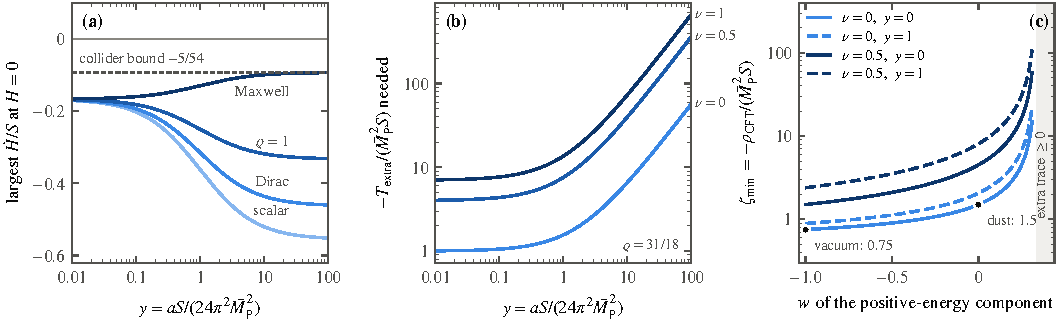
\includegraphics[width=\textwidth]{prd_trace}
\caption{Trace requirements at an anisotropic turning point.
(a)~Largest $\dot H/S$ at a zero of $H$ when all other matter has non-negative trace, Eq.~\eqref{eq:rA-rate}, versus the anomaly strength $y$, for $\varrho=a/c$ of a conformal scalar ($\tfrac13$), a Dirac fermion ($\tfrac{11}{18}$), a Maxwell field ($\tfrac{31}{18}$), and $\varrho=1$; every curve stays below $-5/54$. %
(b)~Least negative extra trace needed for a turning rate $\nu=\dot H/S$ at $\varrho=\tfrac{31}{18}$, Eq.~\eqref{eq:rA-budget}.
(c)~Least negative CFT energy $\zeta_{\min}$, Eq.~\eqref{eq:rA-joint}, when a positive-energy component with equation of state $w$ supplies the trace; for $w\geq1/3$ (shaded) the obstruction applies.}
\label{fig:rA-trace}
\end{figure}

\subsection{The zero-expansion boundary}
\label{rA:hidentity}

The obstruction at $S>0$ is strict, but an isotropic zero of $H$ with $\dot H=0$ is degenerate, and we must exclude a crossing through it.
For this we need the anomaly at general $H$.
Inserting Eqs.~\eqref{eq:rA-W2} and~\eqref{eq:rA-E4} without setting $H=0$, and collecting the terms that do not vanish at $H=0$ into $Q_0+4a\dot HS$, gives
\begin{equation}
\begin{aligned}
cW^2-aE_4&=Q_0+4a\dot H\big(S-6H^2\big)+H\mathcal P,\\
\mathcal P&=4(c+2a)\Tr(u\sigma)+8(c-a)\Tr\sigma^3+(2c+12a)HS-24aH^3 .
\end{aligned}
\label{eq:rA-genH}
\end{equation}
The four terms of $\mathcal P$ come from $4cH\Tr(u\sigma)+8aH\Tr(u\sigma)$, from $8cH\Tr\sigma^3-8aH\Tr\sigma^3$, from $2cH^2S+12aH^2S$ and from $-24aH^4$; the term $-24aH^2\dot H$ joins $4a\dot HS$.
With $R=6\dot H+12H^2+S$ and $b=0$ the traced Einstein equation reads
\begin{equation}
\Big[6\MPbar^2+\frac{a(S-6H^2)}{4\pi^2}\Big]\dot H=-\MPbar^2\big(12H^2+S\big)-\frac{Q_0+H\mathcal P}{16\pi^2}-T_{\rm extra}.
\label{eq:rA-genH-trace}
\end{equation}

\begin{rAlemma}[No degenerate crossing]\label{lem:rA-crossing}
Under the hypotheses of Theorem~\ref{thm:rA-obstruction}, a regular contracting solution cannot cross $H=0$, even at a degenerate zero with $\dot H(t_*)=0$.
\end{rAlemma}

\begin{rAproof}
Near a regular zero of $H$ the bracket on the left of Eq.~\eqref{eq:rA-genH-trace} exceeds $3\MPbar^2$, since it equals $6\MPbar^2+aS/4\pi^2$ at $H=0$ and is continuous.
With $\varrho\leq2$ and $T_{\rm extra}\geq0$ every term on the right except $-H\mathcal P/16\pi^2$ is non-positive, and $\mathcal P$ is bounded on a compact neighborhood of $t_*$.
Hence $\dot H\leq k|H|$ there, for a constant $k$.
If $H$ became positive after a zero at $t_*$, then $d(e^{-kt}H)/dt=e^{-kt}(\dot H-kH)\leq0$ wherever $H>0$, so $e^{-kt}H(t)\leq e^{-kt_*}H(t_*)=0$ on the first interval of positivity, a contradiction.
\end{rAproof}

The lemma completes the proof of Theorem~\ref{thm:rA-obstruction}.
Numerically, Eq.~\eqref{eq:rA-genH} holds to $10^{-12}$ in relative terms for random noncommuting $\sigma$ and $u$ and random $H$, $\dot H$, $a$ and $c$. %

\subsection{What a turning point must supply}
\label{rA:supply}

Allowing any $T_{\rm extra}$, we now ask how negative it must be.
Setting $\dot H=\nu S$ with a turning rate $\nu>0$ in Eq.~\eqref{eq:rA-hdot} and solving for $T_{\rm extra}$ gives $-T_{\rm extra}=\MPbar^2S+Q_0/16\pi^2+6\nu\MPbar^2S(1+y)$.
With the minimal $Q_0$ and the collider bound,
\begin{equation}
-\frac{T_{\rm extra}}{\MPbar^2S}\geq1+6\nu(1+y)+2(2-\varrho)y\geq1+6\nu(1+y)+\frac59y .
\label{eq:rA-budget}
\end{equation}

\paragraph{Who pays.}
Suppose that a positive-energy component with $\bar p=w\rho_w$ supplies the trace, $T_{\rm extra}=-(1-3w)\rho_w$, and the CFT supplies the energy $\rho_{\rm CFT}=-\zeta\MPbar^2S$.
The constraint at the turn, $\rho_w+\rho_{\rm CFT}=-\tfrac12\MPbar^2S$, fixes $\rho_w=(\zeta-\tfrac12)\MPbar^2S$, and Eq.~\eqref{eq:rA-budget} becomes $(\zeta-\tfrac12)(1-3w)\geq1+6\nu(1+y)+5y/9$.
For $w<1/3$ this gives
\begin{equation}
\zeta\geq\frac12+\frac{1+6\nu(1+y)+5y/9}{1-3w}.
\label{eq:rA-joint}
\end{equation}
For $w\geq1/3$ no positive $\rho_w$ satisfies the inequality, and the obstruction applies.
At marginal turning, $\nu\to0$, the least negative CFT energy is $\zeta=\tfrac34+\tfrac{5}{36}y$ for vacuum energy, $w=-1$, and $\tfrac32+\tfrac59y$ for dust, $w=0$ [Fig.~\ref{fig:rA-trace}(c)]. %
Any positive-energy matter with $w<1/3$ can pay for the trace.
Vacuum energy does it most cheaply, while saturating the null energy condition, so the most economical turning point combines a positive potential with a separate source of negative energy.

\paragraph{An exact criterion.}
With $T_{\rm extra}=-4\rho_\Lambda$ and $\rho_\Lambda=3\MPbar^2h^2$, the numerator of Eq.~\eqref{eq:rA-hdot} is $\MPbar^2S+Q_0/16\pi^2-12\MPbar^2h^2$, and Eq.~\eqref{eq:rA-hdot} becomes an exact criterion for every state of the conformal sector:
\begin{equation}
\dot H>0\quad\Longleftrightarrow\quad S_b<12h^2-\frac{Q_0}{16\pi^2\MPbar^2},
\label{eq:rA-exact-criterion}
\end{equation}
where $S_b$ is the shear at the turn.
For a rolling inflaton, $\rho_\phi=K_\phi+V$ and $\bar p_\phi=K_\phi-V$ with $K_\phi=\tfrac12\dot\phi^2$, so $-T_{\rm extra}=4V-2K_\phi$, and the kinetic energy of the inflaton counts against the turn.
For the Casimir turning point of Sec.~\ref{rep:turning} the shear and $Q_0$ vanish at the turn of the isotropic background, and Eq.~\eqref{eq:rA-exact-criterion} holds with a margin $12h^2$; anomalous corrections to it are of relative order $\epsilon^2$, with $\epsilon\simeq3\times10^{-5}$ the small parameter of Sec.~\ref{rep:turning}. %

\paragraph{Beyond the conformal hypothesis.}
Running couplings, masses or minimally coupled scalars break the conformal hypothesis~\cite{CesareSilva:2024nym,CesareSilva:2026zne}, and a healthy $R^2$ term shifts $b$ and requires negative matter energy~\cite{Anderson:1983nq,DeFelice:2010aj}.
The rest of this report takes the most economical route: a positive potential (assumption~\ref{assump:A3}) and the negative Casimir energy of the Standard Model, computed in the next chapter.

\section{Casimir energy of the Standard Model on a three-torus}\label{rep:casimir}

The Standard Model supplies the negative energy of a turning point when its fermions are antiperiodic.
With all three cycles of a cubic torus antiperiodic, its signed Casimir weight is $\NC=+25.515$, whereas periodic fermions give $-30$ (Sec.~\ref{rA:spin}). %
This chapter derives the image sum for twisted free fields from the mode sum (Sec.~\ref{rA:imagesum}), evaluates the lattice sums by an Ewald split (Sec.~\ref{rA:ewald}), assembles the Standard Model weights for every spin structure (Sec.~\ref{rA:spin}), and examines flat holonomies, 't~Hooft flux and the corrections to the field content (Secs.~\ref{rA:holonomy}--\ref{rA:content-corr}).
The energy of the constant modes, which does not depend on the shape and is a fraction $\fzm=0.30$ of the free Casimir energy at the cube, is the subject of Sec.~\ref{rep:zeromodes}, and the turning point that follows, at $\Lb=722\,\MPbar^{-1}$, that of Sec.~\ref{rep:turning}. %

\subsection{Vacuum energy of twisted free fields: the image sum}
\label{rA:imagesum}

\paragraph{Modes.}
On the torus with metric $h_{ij}=L^2G_{ij}$ and coordinates of unit period, a free massless field whose value changes by the phase $e^{2\pi i\vartheta_j}$ around the $j$th cycle has comoving wave vectors $\bm k=2\pi(\bm n+\bm\vartheta)$ with $\bm n\in\mathbb Z^3$.
Its physical frequencies are
\begin{equation}
\omega_{\bm n}=\frac{2\pi}{L}\Big[(\bm n+\bm\vartheta)^{\mathsf T}G^{-1}(\bm n+\bm\vartheta)\Big]^{1/2}.
\label{eq:rA-modes}
\end{equation}
Antiperiodic fermions have $\vartheta_j=\tfrac12$ on the antiperiodic cycles, and a flat gauge holonomy adds the charge times the holonomy phase to $\bm\vartheta$.

\paragraph{From modes to images.}
For one real bosonic degree of freedom the zero-point energy is $E_1=\tfrac12\sum_{\bm n}\omega_{\bm n}$.
Poisson summation, $\sum_{\bm n}f(\bm n+\bm\vartheta)=\sum_{\bm m}\hat f(\bm m)\,e^{2\pi i\bm m\cdot\bm\vartheta}$ with $\hat f(\bm m)=\int d^3\kappa\,f(\bm\kappa)e^{-2\pi i\bm m\cdot\bm\kappa}$, turns the mode sum into a sum over images.
For $f(\bm\kappa)=\tfrac12\omega(\bm\kappa)$ we change variables to the physical wave vector $\bm q=2\pi G^{-1/2}\bm\kappa/L$, whose Jacobian is $d^3\kappa=(L/2\pi)^3d^3q$ because $\det G=1$, and find
\begin{equation}
\hat f(\bm m)=L^3\int\frac{d^3q}{(2\pi)^3}\,\tfrac12|\bm q|\,e^{-i\bm q\cdot\bm x_{\bm m}},\qquad \bm x_{\bm m}=LG^{1/2}\bm m ,
\end{equation}
where $|\bm x_{\bm m}|^2=L^2\,\bm m^{\mathsf T}G\bm m$ is the squared physical length of the closed geodesic in the class $\bm m$.
The Fourier transform of $|\bm q|$ in three dimensions is, away from the origin,
\begin{equation}
\int\frac{d^3q}{(2\pi)^3}\,|\bm q|\,e^{i\bm q\cdot\bm x}=\frac{2}{\pi^{3/2}}\frac{\Gamma(2)}{\Gamma(-\tfrac12)}\frac{1}{|\bm x|^4}=-\frac{1}{\pi^2|\bm x|^4}.
\end{equation}
The term $\bm m=0$ is the energy of the same field in infinite space; it is proportional to the volume and renormalizes the cosmological constant.
The images $\bm m\neq0$ give the finite, regularization-independent part,
\begin{equation}
E_1=-\frac{1}{2\pi^2L}\sum_{\bm m\neq0}\frac{\cos(2\pi\bm\vartheta\cdot\bm m)}{(\bm m^{\mathsf T}G\bm m)^2},
\label{eq:rA-E1}
\end{equation}
after pairing $\bm m$ with $-\bm m$.
A Maxwell field has two polarizations, a Weyl fermion two helicity states with the opposite sign of the zero-point energy, and a real scalar one degree of freedom.

\paragraph{The image sum.}
Summing over fields, the vacuum energy of free massless fields with flat twists $\bm\vartheta_f$ is therefore the image sum~\cite{DeWitt:1979dd,Banach:1979iy,Bellucci:2009jr}
\begin{equation}
\begin{aligned}
E_C&=-\frac{1}{\pi^2L}\sum_{\bm n\neq0}\frac{w_{\bm n}}{(\bm n^{\mathsf T}G\bm n)^2},\\
w_{\bm n}&=\sum_fd_fs_f\cos(2\pi\bm\vartheta_f\cdot\bm n),
\end{aligned}
\label{eq:rA-imagesum}
\end{equation}
with $s_f=+1$ for bosons and $-1$ for fermions, and $d_f=1$ for a Maxwell field, a Weyl fermion or the static graviton and $\tfrac12$ for a real scalar.
Each image $\bm n$ contributes with the weight $w_{\bm n}$, the signed number of degrees of freedom that return to themselves around the closed geodesic $\bm n$.
Untwisted bosons give negative energy.
Periodic fermions ($\bm\vartheta=0$) therefore raise the energy, while antiperiodic fermions lower it~\cite{Arkani-Hamed:2007ryu,Ibanez:2017kvh}, because their images with odd $\sum_jn_j$ change sign; flat gauge holonomies twist charged fields in the same way.
We write $Z_s(G)=\sum'_{\bm n}(\bm n^{\mathsf T}G\bm n)^{-s}$ and $Z_s(G,\bm\vartheta)=\sum'_{\bm n}\cos(2\pi\bm\vartheta\cdot\bm n)(\bm n^{\mathsf T}G\bm n)^{-s}$, so that
\begin{equation}
E_C=-\frac{Z_{\rm eff}(G)}{\pi^2L},\qquad Z_{\rm eff}(G)=\sum_fd_fs_f\,Z_2(G,\bm\vartheta_f).
\label{eq:rA-Zeff}
\end{equation}

\subsection{Lattice constants of the cube}
\label{rA:lattice}

At the cube we write
\begin{equation}
\rho_C=\frac{E_C}{L^3}=-\frac{\NC\rAgam}{L^4},\qquad \rAgam=\frac{Z_2(\rAone)}{\pi^2}=1.6750738,\qquad \NC=\frac{1}{Z_2(\rAone)}\sum_{\bm n\neq0}\frac{w_{\bm n}}{|\bm n|^4},
\label{eq:rA-NC}
\end{equation} %
so that one periodic Maxwell field has $\NC=1$, and the Casimir coefficient of the torus is $C=\NC\rAgam=Z_{\rm eff}(\rAone)/\pi^2$, with $E_C=-C/L$.
For a periodic real scalar this is the familiar $E_C=-\rAgam/(2L)=-0.8375/L$.

On a single circle of length $L$ an antiperiodic field has the image weights $(-1)^n$, and
\begin{equation}
\sum_{n\geq1}\frac{(-1)^n}{n^4}=-\big(1-2^{-3}\big)\zeta(4),
\end{equation}
so an antiperiodic fermion contributes $7/8$ of the periodic magnitude with the opposite sign. %
On the cubic three-torus with all three cycles antiperiodic (AAA) the alternating lattice sum is much weaker:
\begin{equation}
Z_2\big(\rAone,(\tfrac12,\tfrac12,\tfrac12)\big)=\sum_{\bm n\neq0}\frac{(-1)^{n_1+n_2+n_3}}{|\bm n|^4}=-3.8631638, %
\label{eq:rA-aaa-sum}
\end{equation}
so an AAA Weyl fermion contributes $+3.8631638/16.5323160=+0.233673$ to $\NC$, while a periodic one contributes $-1$. %
The reason is a near cancellation between shells.
Images with even $n_1+n_2+n_3$ form the face-centered sublattice and contribute $Z_{\rm even}=6.3346$, and the odd images contribute $Z_{\rm odd}=10.1977$; the alternating sum is their difference. %
The six nearest images, $|\bm n|=1$, are odd and dominate, while the twelve next ones, $|\bm n|^2=2$, are even and cancel half of them.

\subsection{Ewald evaluation of the lattice sums}
\label{rA:ewald}

The sums of Eq.~\eqref{eq:rA-imagesum} converge slowly, and their shape derivatives more slowly still.
We evaluate $Z_2(G,\bm\vartheta)$ by an Ewald split.
With $Q_{\bm n}=\bm n^{\mathsf T}G\bm n$ we write $Q^{-2}=\int_0^\infty t\,e^{-tQ}\,dt$ and split the integral at $t=\pi$.
The upper part is elementary, $\int_\pi^\infty t\,e^{-tQ}dt=(1+\pi Q)e^{-\pi Q}/Q^2$.
In the lower part we complete the sum with the term $\bm n=0$, which contributes $\int_0^\pi t\,dt=\pi^2/2$ and is subtracted again, and apply Poisson summation to the Gaussian,
\begin{equation}
\sum_{\bm n}\cos(2\pi\bm\vartheta\cdot\bm n)\,e^{-tQ_{\bm n}}=\Big(\frac\pi t\Big)^{3/2}\frac{1}{\sqrt{\det G}}\sum_{\bm m}e^{-\pi^2P_{\bm m}/t},\qquad P_{\bm m}=(\bm m-\bm\vartheta)^{\mathsf T}G^{-1}(\bm m-\bm\vartheta).
\end{equation}
For $P_{\bm m}>0$ the substitution $t=\pi^2P_{\bm m}/x$ gives $\int_0^\pi t\,(\pi/t)^{3/2}e^{-\pi^2P/t}dt=\pi^{5/2}\sqrt P\,\Gamma(-\tfrac12,\pi P)$, and for $P_{\bm m}=0$, which occurs only for integer $\bm\vartheta$, the integral is $\pi^{3/2}\int_0^\pi t^{-1/2}dt=2\pi^2$.
Altogether
\begin{equation}
\begin{aligned}
Z_2={}&\sum_{\bm n\neq0}\cos(2\pi\bm\vartheta\cdot\bm n)\frac{(1+\pi Q_{\bm n})e^{-\pi Q_{\bm n}}}{Q_{\bm n}^2}-\frac{\pi^2}{2}\\
&+\frac{\pi^2}{\sqrt{\det G}}\Big[\sum_{P_{\bm m}>0}\sqrt{\pi P_{\bm m}}\,\Gamma(-\tfrac12,\pi P_{\bm m})+2\,\delta_{\bm\vartheta\in\mathbb Z^3}\Big],
\end{aligned}
\label{eq:rA-ewald}
\end{equation}
with $\Gamma(-\tfrac12,x)=2x^{-1/2}e^{-x}-2\sqrt\pi\,{\rm erfc}\sqrt x$.
Both sums now converge like Gaussians.
At the cube this gives $Z_2(\rAone,0)=16.5323159598$ and $Z_2(\rAone,(\tfrac12,\tfrac12,\tfrac12))=-3.8631638072$; a direct sum of the alternating series over $|n_i|\leq60$ agrees to $10^{-8}$. %
A separate implementation with $|n_i|,|m_i|\leq7$ reproduces both values to all printed digits. %
The same code, with derivatives of Eq.~\eqref{eq:rA-ewald} along the shape geodesics, gives the shape Hessians below and the shape forces of the nonlinear evolution in Sec.~\ref{rep:quantum-shape}.

\subsection{Spin structures}
\label{rA:spin}

At the turning point all Standard Model masses are negligible (Sec.~\ref{rA:scope}).
In the units of Eq.~\eqref{eq:rA-imagesum} the content of Sec.~\ref{rA:content} has $B=12+2+1=15$ for the gauge vectors, the Higgs doublet and the static graviton, and $F=45$ for the Weyl fermions. %
For the Standard Model plus the static graviton, $Z_{\rm eff}=15Z_2(G,0)-45Z_2(G,\bm\vartheta_F)$. %
At the cube, with $Z_2(\rAone,\bm\vartheta_F)/Z_2(\rAone)=1$ for periodic and $-0.233673$ for AAA fermions,
\begin{equation}
\begin{aligned}
\NC^{\rm PPP}&=15-45=-30,\\ %
\NC^{\rm AAA}&=15+45\times0.233673=+25.515 . %
\end{aligned}
\label{eq:rA-NCSM}
\end{equation}
The Casimir coefficient of the AAA Standard Model is $C=\NC\rAgam=42.74$. %
With periodic fermions and trivial holonomies the Standard Model Casimir energy is positive.
A torus then expands from a small size but cannot turn around, which is the empty-torus scenario of Ref.~\cite{Fornal:2026qfq}.
With fermions antiperiodic around all three edges of the cube the energy is negative and supports a turning point without additional light fields [Fig.~\ref{fig:rA-casimir-shape}(a)].

\paragraph{The eight spin structures.}
A spin structure assigns P or A to each of the three cycles.
The eight spin structures of $T^3$ fall into two classes under $SL(3,\mathbb Z)$, the periodic one and the seven others, because a change of lattice basis maps any non-periodic assignment into any other; on the cube the latter differ in which edges are antiperiodic.
At trivial holonomy one or two antiperiodic edges give $\NC=13.1$ and $20.9$, and the cube is not stationary. %
For these structures trivial holonomy is not the vacuum of the zero modes: the one-loop potential puts an $SU(3)$ centre holonomy on each periodic edge, which raises $\NC$ to $21.07$ (one antiperiodic edge) and $23.67$ (two). %
Scanning the hypercharge and $SU(2)$ Cartan directions together with the $SU(3)$ centre, we find that under this holonomy the quarks are twisted by $\pm1/3$ along each periodic edge while the Higgs doublet and the gauge fields are not.
The cube is not stationary, but the energy is stationary at a tetragonal shape, with the antiperiodic edge $28\%$ longer than the periodic ones for PPA and the periodic edge $17\%$ shorter than the antiperiodic ones for PAA. %
There $\NC=19.72$ and $22.84$, and both aspect directions are unstable, as they are for AAA at the cube. %
These sectors also turn around, and Sec.~\ref{rep:h-universality} returns to their Higgs zero mode.
The AAA assignment keeps the cube stationary, gives the largest weight and leaves the holonomies trivial; it is our benchmark (assumption~\ref{assump:A1}), and the shape predictions of Secs.~\ref{rep:quantum-shape} and~\ref{rep:sky} refer to it.

\paragraph{Shape Hessians.}
At a stationary cube the Hessian of $Z_{\rm eff}$ in the coordinates of Eq.~\eqref{eq:rA-betaparam} is diagonal in the representations $E$ and $T_2$, with eigenvalues $\lambda_E$ (twice) and $\lambda_{T_2}$ (three times).
Table~\ref{tab:rA-spin} lists them.
For AAA the normalized stiffnesses $\kappa_A=3\lambda_A/Z_{\rm eff}$ of Sec.~\ref{rep:shape} are $\kappa_E=13.5286$ and $\kappa_{T_2}=-6.3524$, with $\sum_A\kappa_A=2\kappa_E+3\kappa_{T_2}=8.0000$, and $\Tr\,{\rm Hess}\,Z_{\rm eff}=\tfrac83Z_{\rm eff}$ holds to $10^{-8}$ for all eight structures. %
For PPP the trace identity reads $2(-991.56)+3(220.18)=\tfrac83(-30)Z_2(\rAone)$.
Section~\ref{rep:shape} derives the identity and explains why it makes a negative Casimir energy unable to hold any shape.

\begin{table}[tbp]
\centering
\caption{Standard Model plus the static graviton on the cubic three-torus at trivial holonomy, for fermion spin structures with periodic (P) and antiperiodic (A) cycles: signed Casimir weight, whether the cube is stationary, and the Hessian eigenvalues of $Z_{\rm eff}$ in the aspect ($E$) and angle ($T_2$) directions, with their multiplicities.}
\label{tab:rA-spin}
\begin{tabular}{lcccc}
\toprule
spin structure & $\NC$ & stationary & $\lambda_E$ ($\times2$) & $\lambda_{T_2}$ ($\times3$)\\
\midrule
PPP & $-30.00$ & yes & $-991.56$ & $+220.18$\\ %
PPA & $+13.12$ & no & & \\ %
PAA & $+20.87$ & no & & \\ %
AAA & $+25.515$ & yes & $+1902.24$ & $-893.20$\\ %
\bottomrule
\end{tabular}
\end{table}

\paragraph{Why antiperiodic cycles.}
Antiperiodic cycles are natural in a quantum origin, because a cycle that caps off smoothly in a Euclidean geometry must carry them~\cite{GarciaEtxebarria:2020xsr}.
The smooth no-boundary fillings of $T^3$ cap one primitive cycle~\cite{Godet:2026gqw}, which requires a non-periodic spin structure, although not specifically AAA.
The sign mechanism is old.
Antiperiodic spinors entered the Casimir energy of a created torus in the work of Zel'dovich and Starobinsky~\cite{Zeldovich:1984vk} (see Ref.~\cite{Guth:2025dal}), and twisted fields were used to make the Casimir energy of supergravity on $T^3$ negative for quantum creation~\cite{Goncharov:1985gi,Linde:2004nz}.
On a circle the Standard Model is often studied with both spin structures~\cite{Arkani-Hamed:2007ryu,Ibanez:2017kvh}.
The periodic Standard Model on $T^3$ has been studied for general shapes~\cite{Fornal:2011tw,Fornal:2026qfq}; here we compute the total for the non-periodic spin structures, its sign and its shape Hessian at the cube (Table~\ref{tab:rA-spin}).

\begin{figure}[tbp]
\centering
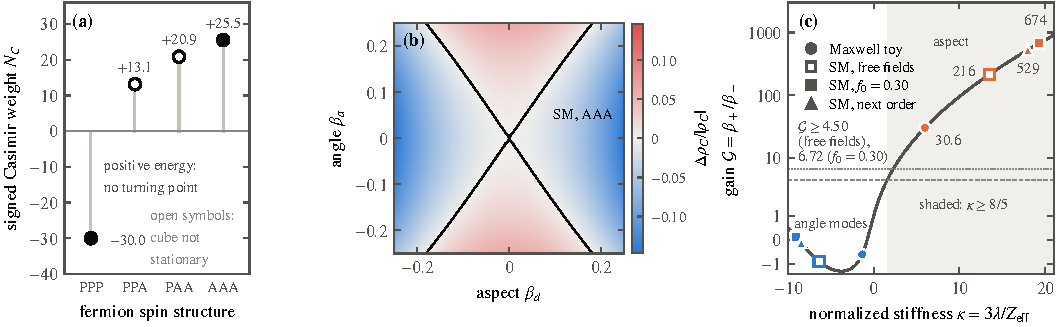
\includegraphics[width=\textwidth]{prd_casimir_shape}
\caption{Standard Model Casimir energy and its shape instability.
(a)~Signed Casimir weight $\NC$ of the high-energy Standard Model plus the static graviton on the cubic torus at trivial holonomy, for periodic (P) or antiperiodic (A) fermion cycles; filled: stationary cube.
(b)~Fractional change of the AAA Casimir energy density on the slice $G=\exp(2\beta_dX_d+2\beta_aX_{12})$; aspect deformations lower it, angle deformations raise it.
(c)~Gain of a linear shape mode versus normalized stiffness: Maxwell toy (circles), Standard Model with free fields (open squares), with $\fzm=0.30$ (filled squares) and at next order (triangles); shaded: $\kappa\geq8/5$ (Sec.~\ref{rep:shape}).}
\label{fig:rA-casimir-shape}
\end{figure}

\subsection{Flat gauge holonomies}
\label{rA:holonomy}

Flat gauge holonomies twist charged fields like spin structures, and charged fields give them a one-loop potential~\cite{Hosotani:1983xw}.
They enter Eq.~\eqref{eq:rA-imagesum} as additional twists, $\vartheta_i=Yg_i$ for a hypercharge holonomy $\bm g$ acting on a field of hypercharge $Y$, and $\vartheta_i=\pm k_i/3$ on (anti)triplets for an $SU(3)$ centre holonomy with integers $k_i$.
With periodic fermions the centre holonomies $\bm k=(1,1,1)$ and $(1,0,0)$ give $\NC=11.19$ and $0.56$, and the hypercharge holonomy $\bm g=g(1,1,1)$ gives $7.13$ at $g=3/2$ and at most $17.79$. %
So with periodic fermions an $SU(3)$ centre holonomy on all three cycles gives $\NC=+11.2$, and a hypercharge holonomy up to $+17.8$, and negative energy does not require antiperiodic fermions. %
These sectors break the cubic symmetry, and in the periodic case the energy decreases away from trivial holonomy.
For AAA the centre holonomies give $9.86$ and $22.74$, and $\NC$ along the hypercharge direction is maximal, $25.515$, at $g=0$. %
Trivial holonomy therefore maximizes $\NC$ along the hypercharge direction, and centre holonomies on one or three cycles lower it to $22.7$ and $9.9$, so the benchmark is stable against these deformations. %

\subsection{Sectors with 't~Hooft flux}
\label{rA:thooft}

In sectors with 't~Hooft flux the Standard Model fields are single valued only if a nontrivial $SU(3)$ or $SU(2)$ twist comes with a hypercharge flux $\Phi_Y$, and the smallest one is $|\Phi_Y|=2\pi$.
A constant hypercharge field strength with flux $\Phi_Y$ through a face of the cube has $F_{12}=\Phi_Y$ in coordinates of unit period, and its classical energy is
\begin{equation}
E_{\rm flux}=\frac{1}{2g_Y^2}\int d^3x\,\sqrt h\,h^{11}h^{22}F_{12}^2=\frac{\Phi_Y^2}{2g_Y^2L}\geq\frac{2\pi^2}{g_Y^2L}=\frac{100.7}{L}
\label{eq:rA-flux}
\end{equation}
at $g_Y(\mub)=0.443$. %
This is $2.36$ times the AAA Casimir energy $C/L$. %
A turn would need $\NC>2\pi^2/(g_Y^2\rAgam)=60$, whereas the Standard Model content gives at most $25.5$ for any flat twist, so these sectors cannot turn around. %

\subsection{Corrections to the field content}
\label{rA:content-corr}

Two smaller corrections concern the content.
The inflaton fluctuation is light at the turning point and adds $\tfrac12$ to $\NC$, which lowers the shape fossil of Sec.~\ref{rep:quantum-shape} by $2\%$ for free fields and by $3.5\%$ with the zero-mode energy of Sec.~\ref{rep:zeromodes}. %
Three right-handed neutrinos lighter than $2\pi/\Lb$ would add $0.70$, since three antiperiodic Weyl fermions contribute $3\times0.233673$. %
We keep the content of Eq.~\eqref{eq:rA-NCSM} and carry these effects in the error budgets of Secs.~\ref{rep:h-budget} and~\ref{rep:quantum-shape}.
Perturbative interactions of the nonzero modes correct $\NC$ by a relative amount of order $g^2/16\pi^2$.
The interactions of the constant modes are not perturbative at this size and are treated next.

\section{Zero modes of the Standard Model}\label{rep:zeromodes}

The constant modes of the gauge and Higgs fields are not free fields, and their energy is not part of the image sum of Sec.~\ref{rep:casimir}.
We show that their ground energy $Q/L$ is positive and independent of the shape at fixed volume, and that it uses up a fraction
\begin{equation}
\fzm\equiv Q/C=0.30 %
\label{eq:rA-fzero}
\end{equation}
of the free Casimir energy, between the lower bound $0.26$ and the Gaussian variational bound $0.31$. %
The Higgs zero mode is held mainly by the zero-point fluctuations of the electroweak gauge modes.
At next order in the small-volume expansion the fraction falls to about $0.28$ and the zero modes acquire a weak shape dependence.
Sections~\ref{rA:zm-hamiltonian}--\ref{rA:zm-isospectral} derive the Hamiltonian and its shape independence, Secs.~\ref{rA:zm-bounds}--\ref{rA:zm-couplings} its ground energy, Secs.~\ref{rA:zm-nextorder}--\ref{rA:zm-shape} the next order, and Sec.~\ref{rA:zm-consequences} the consequences for the background and for the Higgs zero mode.

\subsection{The constant modes and their Hamiltonian}
\label{rA:zm-hamiltonian}

Each of the twelve gauge fields has three constant modes, one per cycle, and the Higgs doublet has four.
Their state is not fixed by the Hadamard condition~\cite{Negro:2026ooh}, which constrains only the short-distance behavior, and their nonlinear self-interaction gives their ground state a finite energy~\cite{Luscher:1982uv,Luscher:1982ma}.
For antiperiodic fermions the vacuum lies at trivial holonomy and is unique~\cite{vanBaal:1988va}, and the AAA fermions themselves have no constant modes.

\paragraph{Reduction of the action.}
We use the covariant derivative $D=\partial-i(A^aT_a+YB)$ with ${\rm tr}\,T_aT_b=\tfrac12\delta_{ab}$, temporal gauge, and constant modes
\begin{equation}
A^a_i=g\,x^a_i(t),\qquad B_i=g_Y\,w_i(t)
\label{eq:rA-xw}
\end{equation}
in coordinates of unit period, with $g=g_3$ or $g_2$ for the non-abelian factors.
For constant spatial components the field strength is $F^a_{0i}=\dot A^a_i$ and $F^a_{ij}=f^{abc}A^b_iA^c_j=g^2F^a_{ij}[x]$, with $F^a_{ij}[x]=f^{abc}x^b_ix^c_j$.
With $\sqrt{-g}=L^3$ and $g^{ij}=G^{ij}/L^2$ the Yang--Mills action $-\frac{1}{4g^2}\int\sqrt{-g}\,F^a_{\mu\nu}F^{a\mu\nu}$ of each gauge factor reduces to
\begin{equation}
L_{\rm YM}=\frac{L}{2}\,G^{ij}\dot x_i\cdot\dot x_j-\frac{g^2}{4L}\,G^{ik}G^{jl}F_{ij}[x]\cdot F_{kl}[x],
\end{equation}
where the dot product sums over the adjoint index.
The constant Higgs doublet enters as $\Phi/L$, with $\Phi=(\phi_0+i\phi_1,\phi_2+i\phi_3)/\sqrt2$ and $r=|\bm\phi|$, so that $\Phi^\dagger\Phi=r^2/2$.
At fixed volume its kinetic term is $L\,\dot\Phi^\dagger\dot\Phi=\tfrac{L}{2}\sum_a\dot\phi_a^2$.
Its gradient term, $-\sqrt{-g}\,g^{ij}(D_i\Phi)^\dagger D_j\Phi$ with $D_i\Phi=-iM_i\Phi/L$ and
\begin{equation}
M_i=g_2\,x_i\cdot T+g_YY\,w_i ,
\end{equation}
contributes the potential $G^{ij}\Phi^\dagger M_iM_j\Phi/L$, and the quartic contributes $\lambda(\Phi^\dagger\Phi)^2/L$.
The Legendre transform, with momenta $\pi_i=LG^{ij}\dot x_j$, $\pi^w_i=LG^{ij}\dot w_j$ and $p_a=L\dot\phi_a$, gives the zero-mode Hamiltonian
\begin{equation}
\begin{aligned}
L\mathcal H_0={}&\sum_{\rm G}\Big[\tfrac12G_{ij}\,\pi_i\cdot\pi_j+\frac{g^2}{4}G^{ik}G^{jl}F_{ij}\cdot F_{kl}\Big]\\
&+\tfrac12G_{ij}\,\pi^w_i\pi^w_j+\tfrac12p_\Phi^2\\
&+G^{ij}\Phi^\dagger M_iM_j\Phi+\lambda(\Phi^\dagger\Phi)^2,
\end{aligned}
\label{eq:rA-H0}
\end{equation}
where the sum runs over the gauge factors $SU(3)$ and $SU(2)$, $F^a_{ij}=f^{abc}x^b_ix^c_j$, and $p_\Phi^2$ sums over the four real components $\phi_a$.
The Gauss law, $f^{abc}x^b_i\pi^c_i$ for each non-abelian factor plus the Higgs charge density, annihilates physical states.
The term $\lambda v^2\Phi^\dagger\Phi$ of the potential is negligible at $\mub$ and is omitted.

\subsection{Isospectrality}
\label{rA:zm-isospectral}

\begin{rAprop}[Shape independence]\label{prop:rA-isospectral}
On the local domain of the constant modes, the Hamiltonian~\eqref{eq:rA-H0} at shape $G$ is unitarily equivalent to the one at the cube.
Its whole local spectrum, not only the ground energy, is therefore independent of the shape at fixed volume.
\end{rAprop}

\begin{rAproof}
Write $G=SS^{\mathsf T}$ with $\det S=1$ and define the canonical map
\begin{equation}
x_i=S_{ij}\tilde x_j,\qquad w_i=S_{ij}\tilde w_j,\qquad \pi=S^{-\mathsf T}\tilde\pi,\qquad \pi^w=S^{-\mathsf T}\tilde\pi^w,
\label{eq:rA-isomap}
\end{equation}
with $\Phi$ unchanged.
The kinetic terms become $\pi^{\mathsf T}G\pi=\tilde\pi^{\mathsf T}S^{-1}SS^{\mathsf T}S^{-\mathsf T}\tilde\pi=\tilde\pi^2$.
The field strength is bilinear, $F_{ij}[x]=S_{ia}S_{jb}F_{ab}[\tilde x]$, and $S^{\mathsf T}G^{-1}S=\rAone$, so $G^{ik}G^{jl}F_{ij}\cdot F_{kl}=F[\tilde x]^2$.
Since $M_i$ is linear in $(x,w)$, $M_i(x,w)=S_{ij}M_j(\tilde x,\tilde w)$, and the same identity gives $G^{ij}\Phi^\dagger M_iM_j\Phi=\sum_j|M_j(\tilde x,\tilde w)\Phi|^2$.
The Gauss generators are unchanged, $\sum_ix_i^b\pi_i^c=\tilde x^b\cdot\tilde\pi^c$, and the Jacobian of the configuration-space map is $\det(\rAone\otimes S)\det S=1$, so the flat Laplacian of the kinetic term is preserved.
The map is therefore unitary on the local domain and carries $\mathcal H_0(G)$ into $\mathcal H_0(\rAone)$.
\end{rAproof}

We checked this exactly for a rational $S$ and numerically for 200 random $S$, to $2\times10^{-14}$. %
The ground energy $Q/L$ is therefore a positive constant on the space of shapes at fixed volume.
Only global features depend on the shape: the lattice of large holonomies is not invariant under the map, so their identification, tunneling between them and the matching to the nonzero modes can depend on the shape; for AAA fermions the ground state sits at trivial holonomy~\cite{vanBaal:1988va}, far from the copies (Sec.~\ref{rA:zm-consequences}).

\subsection{Small-volume scaling and bounds}
\label{rA:zm-bounds}

\paragraph{Scaling.}
At the cube the rescaling $x=g^{-1/3}y$, $\pi_x=g^{1/3}\pi_y$ turns the gauge part of each factor into
\begin{equation}
\tfrac12\pi_x^2+\frac{g^2}{4}F[x]^2=g^{2/3}\Big(\tfrac12\pi_y^2+\tfrac14F[y]^2\Big),
\end{equation}
whose ground energy defines $\epsilon_N$ for $SU(N)$.
At leading order of the small-volume expansion the pure-gauge part of $Q$ is therefore $\epsilon_3g_3^{2/3}+\epsilon_2g_2^{2/3}$, with $\epsilon_2=4.1167$~\cite{Luscher:1983gm} and $\epsilon_3=12.587$~\cite{Weisz:1986vu,Pavel:2021mxn}, independent of the fermions at this order~\cite{vanBaal:1988va}. %
With $g_3\simeq0.54$, $g_2\simeq0.53$ and $g_Y\simeq0.44$ at $\mub$, this is $26\%$ of the free Casimir coefficient $C=\NC\rAgam=42.74$. %

\paragraph{Lower bound.}
Write the electroweak part as $\mathcal H_{\rm EW}=\mathcal H_{SU(2)}\otimes\rAone+K$, where $K$ contains the hypercharge and Higgs kinetic terms, the Higgs gradient term and the quartic.
For $\lambda\geq0$ every term of $K$ is non-negative, $K\geq0$, so ${\rm inf\,spec}\,\mathcal H_{\rm EW}\geq\epsilon_2g_2^{2/3}/L$.
Restricting to gauge-invariant states can only raise the infimum, so
\begin{equation}
Q\geq\epsilon_2g_2^{2/3}+\epsilon_3g_3^{2/3}\qquad(\lambda\geq0).
\end{equation}
Because $\epsilon_3$ is a variational value~\cite{Weisz:1986vu,Pavel:2021mxn}, confirmed by the Monte Carlo below to $2\times10^{-4}$, this bound is numerical rather than rigorous. %
For $\lambda\geq0$ the ground state exists because the zero-point energy lifts the flat valleys of the potential, and it is unique and positive because $e^{-t\mathcal H_0}$ is positivity improving on the connected configuration space; it is therefore gauge invariant.
For $\lambda<0$ the Higgs direction is unbounded below and the ground state becomes a resonance, which Secs.~\ref{rep:h-matching} and~\ref{rep:h-reduced} treat.

\paragraph{Gaussian upper bound.}
The Gaussian
\begin{equation}
\psi\propto\exp\big[-\tfrac12\big(\alpha\,x^2+\beta\,w^2+z\,r^2\big)\big]
\end{equation}
for the $SU(2)$, hypercharge and Higgs zero modes has $\langle(x^a_i)^2\rangle=1/2\alpha$ for each of the nine $SU(2)$ components, $\langle w_i^2\rangle=1/2\beta$ for each of the three hypercharge components and $\langle\phi_a^2\rangle=1/2z$ for each of the four Higgs components.
Its energy follows term by term.
The kinetic terms give $\tfrac12\cdot9\cdot\tfrac\alpha2+\tfrac12\cdot3\cdot\tfrac\beta2+\tfrac12\cdot4\cdot\tfrac z2$.
The magnetic term gives $\tfrac{g_2^2}{4}\langle F\cdot F\rangle$ with $\langle F^a_{ij}F^a_{ij}\rangle=\sum_{i\neq j}\epsilon^{abc}\epsilon^{abc}/(2\alpha)^2=6\cdot6/4\alpha^2$.
The Higgs gradient term gives $g_2^2\sum_i\langle(x_i\cdot T)^2\rangle\langle\Phi^\dagger\Phi\rangle=g_2^2\cdot3\cdot\tfrac34\cdot\tfrac1{2\alpha}\cdot\tfrac1z$, using the doublet Casimir $T^aT^a=\tfrac34$ and $\langle\Phi^\dagger\Phi\rangle=\tfrac12\langle r^2\rangle=1/z$, and the hypercharge term the analogous $g_Y^2Y_H^2\cdot\tfrac3{2\beta}\cdot\tfrac1z$ with $Y_H=\tfrac12$.
The quartic gives $\tfrac\lambda4\langle r^4\rangle=\tfrac\lambda4\cdot\tfrac{6}{z^2}$.
Altogether the upper bound is
\begin{equation}
LE=\tfrac94\alpha+\tfrac34\beta+z+\frac{9g_2^2}{4\alpha^2}+\frac{9g_2^2}{8\alpha z}+\frac{3g_Y^2}{8\beta z}+\frac{3\lambda}{2z^2},
\label{eq:rA-gauss-bound}
\end{equation}
to be minimized over $\alpha$, $\beta$ and $z$.
For $SU(N)$ alone the Gaussian energy is $\tfrac34(N^2-1)\alpha+\tfrac38N(N^2-1)g^2/\alpha^2$; its minimum, at $\alpha^3=Ng^2$, is $\tfrac98(N^2-1)N^{1/3}g^{2/3}$, that is $4.252$ and $12.980$ in units of $g^{2/3}$ for $N=2$ and $3$, $3\%$ above $\epsilon_2$ and $\epsilon_3$. %

\subsection{Diffusion Monte Carlo}
\label{rA:zm-dmc}

For $\lambda\geq0$ the ground state has no nodes, so importance-sampled diffusion Monte Carlo (DMC), guided by the optimal Gaussian, gives the exact local ground energy up to statistical and time-step errors.
Walkers diffuse in the sixteen-dimensional configuration space of the $SU(2)$, hypercharge and Higgs modes with the drift of the guiding Gaussian and branch with the local energy.
We used $10^4$ walkers and time steps $0.04$, $0.02$ and $0.01$, down to $0.005$ for the checks, with linear extrapolation to zero step. %
The method reproduces the certified ground energy $2.1407$ of the four-dimensional quartic oscillator $\tfrac12p^2+\tfrac14(r^2)^2$ as $2.1402(5)$, $\epsilon_2=4.116720$ as $4.1171(14)$ and $\epsilon_3=12.5868$ as $12.5869(22)$. %
With the couplings of Sec.~\ref{rA:zm-couplings}, the coupled electroweak sector has $LE_{\rm EW}=4.4478(13)$ at $\lambda=0$ and $4.4750(17)$ at $\lambda=0.01$, so $Q=12.790$ and $12.818$, and $\fzm=0.2993$ and $0.2999$. %
At $\lambda=0.1$ the fraction is $0.3043$, and $g_2=g_3=0.5$, $g_Y=0.46$ give $0.2878$ at $\lambda=0.01$. %
The pure-gauge bound gives $\fzm\geq0.2580$ and the Gaussian bound $\fzm\leq0.3083$ at $\lambda=0.01$. %
A diffusion Monte Carlo computation of the coupled $SU(2)\times U(1)\times$Higgs ground state therefore gives $Q=12.8$ and Eq.~\eqref{eq:rA-fzero}. %

\paragraph{The Higgs zero mode is held by the gauge modes.}
At $\lambda=0.01$ the hypercharge and Higgs modes add $1.78/L$ to the $SU(2)$ energy, $3.9$ times the energy $2.1407\lambda^{1/3}/L=0.46/L$ of a decoupled quartic oscillator $\tfrac12p_\Phi^2+\lambda(\Phi^\dagger\Phi)^2$. %
Together with hypercharge, the Higgs zero mode raises the $SU(2)$ energy by about four times what a decoupled quartic oscillator would contribute at the same $\lambda$: it is confined mainly by the zero-point fluctuations of the gauge modes through the term $G^{ij}\Phi^\dagger M_iM_j\Phi$, which acts as a mass $\propto g_2^2\langle x^2\rangle$ for $r$. %
The fraction depends weakly on $\lambda$.
It is $0.2993$, $0.2999$ and $0.3043$ for $\lambda=0$, $0.01$ and $0.1$; at the Standard Model value $\lambda(\mub)=-0.0098$, where the Higgs zero mode is a narrow resonance (Secs.~\ref{rep:h-matching}--\ref{rep:h-reduced}), the real part of the resonance energy lowers $Q$ by about $0.08$ relative to $\lambda=0.01$, which gives $\fzm=0.298$. %

\subsection{Couplings}
\label{rA:zm-couplings}

The values above use one-loop couplings at $1/\Lb$, $g_2=0.5268$, $g_3=0.5396$ and $g_Y=0.4415$, with $Y_H=\tfrac12$; the top Yukawa coupling of this set is $y_t=0.4585$. %
The NNLO couplings of assumption~\ref{assump:A2} at $\mub$ are $g_2=0.5278$, $g_3=0.5357$ and $g_Y=0.4428$, within $0.8\%$ of these. %
At this order the zero-mode energies scale as $g^{2/3}$, so the difference moves $\fzm$ by less than $0.001$. %
Taking $\mu=2\pi/\Lb$ instead of $1/\Lb$ lowers $\fzm$ by $0.003$, and determining $\Lb$ self-consistently from $(1-\fzm)C$ changes it by $10^{-4}$. %

\subsection{Next order: the one-loop holonomy potential}
\label{rA:zm-nextorder}

At $\mathcal O(g^{4/3})$ the zero modes feel the curvature of the one-loop potential that the nonzero modes of charged fields create for constant connections~\cite{Luscher:1982ma,vanBaal:1988va} (Fig.~\ref{fig:rA-holonomy-loop}).
A constant connection along the generator $T^a$ shifts the twist of a charged field, $\bm\vartheta\to\bm\vartheta+\bm A\,q/2\pi$ for a charge $q$, so the curvature follows from the twist dependence of the image sum~\eqref{eq:rA-E1}.
Differentiating twice under the sum gives a factor $-(2\pi)^2n_in_j$, and at the cube the cubic average $\sum'n_in_jf(|\bm n|)=\tfrac13\delta_{ij}\sum'|\bm n|^2f(|\bm n|)$ turns $(\bm n^{\mathsf T}\bm n)^{-2}$ into $(\bm n^{\mathsf T}\bm n)^{-1}$.
A field with weight $d_f$, statistics $s_f$, twist $\bm\vartheta_f$ and ${\rm tr}_f\,T^aT^b=t_f\delta^{ab}$ ($t_f=Y^2$ for hypercharge) therefore contributes
\begin{equation}
L\frac{\partial^2E}{\partial A^a_i\partial A^b_j}\bigg|_0=\frac{\delta^{ab}\delta_{ij}}{3\pi^2}\sum_fd_fs_ft_f\,Z_{\rAone}(1;\bm\vartheta_f),
\label{eq:rA-holonomy-curvature}
\end{equation}
where $Z_G(s;\bm\vartheta)=\sum'\cos(2\pi\bm\vartheta\cdot\bm n)(\bm n^{\mathsf T}G\bm n)^{-s}$ is continued analytically to $s=1$.
Its values are $Z_{\rAone}(1;0)=-8.913633$, with the slow-mode cusp removed, and $Z_{\rAone}(1;\bm\vartheta_{\rm AAA})=-2.519356$. %
For periodic fields at trivial holonomy the charged mode with $\bm n+\bm\vartheta=0$ would make the potential non-analytic; that mode is part of the zero-mode Hamiltonian and is removed from the sum.
For $SU(3)$ with six Dirac flavours this reproduces van Baal's coefficient $-0.19631$~\cite{vanBaal:1988va}. %
For the Standard Model the curvatures are $-0.393$ for $SU(3)$, $-0.242$ for $SU(2)$, including the nonzero modes of the Higgs doublet, and $+0.700$ for hypercharge. %
The AAA fermions confine hypercharge, whose curvature is positive, while the periodic bosons dominate the negative non-abelian curvatures.

\begin{figure}[tbp]
\centering
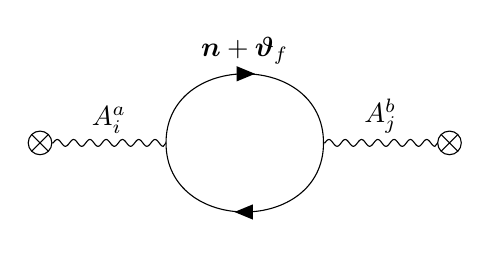
\begin{tikzpicture}
\begin{feynman}
\vertex[crossed dot] (x1) at (-2.6,0) {};
\vertex (a) at (-1.0,0);
\vertex (b) at (1.0,0);
\vertex[crossed dot] (x2) at (2.6,0) {};
\diagram*{
(x1) -- [photon, edge label=\(A^a_i\)] (a),
(a) -- [fermion, half left, edge label=\(\bm n+\bm\vartheta_f\)] (b),
(b) -- [fermion, half left] (a),
(b) -- [photon, edge label=\(A^b_j\)] (x2),
};
\end{feynman}
\end{tikzpicture}
\caption{The one-loop curvature of the holonomy potential, Eq.~\eqref{eq:rA-holonomy-curvature}.
The loop runs over the nonzero modes of every charged field, with momenta $2\pi(\bm n+\bm\vartheta_f)$ on the torus; the crossed dots are insertions of the constant gauge zero modes.
Charged scalars and vectors contribute in addition through the seagull vertex with both insertions at one point.
Summed over the modes, the diagram is the second twist derivative of the image sum, which turns the $s=2$ Epstein function of the Casimir energy into the $s=1$ function.}
\label{fig:rA-holonomy-loop}
\end{figure}

\paragraph{First-order shift of the zero-mode energy.}
In first-order perturbation theory the curvature shifts the ground energy by $\Delta Q=\tfrac12\sum_{\rm G}M_{\rm G}\langle A^2\rangle_{\rm G}$, where $M_{\rm G}$ is the curvature per component and $\langle A^2\rangle_{\rm G}$ the summed spread of the ground state of factor G.
With the Gaussian spreads $\langle A^2\rangle=3.66$ for $SU(3)$ ($3.77$ from the virial theorem) and $1.40$ for $SU(2)$, and $\langle B^2\rangle=0.82$, the first-order shift is $\Delta Q=-0.72-0.17+0.29=-0.60$, or $\Delta\fzm=-0.014$; a virial spread for $SU(3)$ gives $-0.015$. %
The gluon and $W$ modes lower $\fzm$ by $0.021$, and hypercharge, which the AAA fermions confine, raises it by $0.007$. %
The dependence of the full one-loop potential on the Higgs radius $r$ enters the Higgs zero mode as cross terms (Sec.~\ref{rep:h-cross}).
The nonzero modes also give the Higgs zero mode a mass, which Sec.~\ref{rep:h-matching} treats together with the one-loop finite-volume potential along $r$.
In the Gaussian estimate used here this mass lowers $\fzm$ by a further $0.003$, and the NNLO top Yukawa coupling at $\mub$, $y_t=0.428$, changes that by $0.0003$. %
Together the first-order terms give $\fzm\simeq0.28$. %

\paragraph{Convergence of the small-volume expansion.}
The expansion parameter $g^{2/3}\simeq0.66$ is not small, but the published $SU(2)$ series converges quickly at this coupling. %
For three flavours its corrections are $-11\%$, $-0.4\%$ and $-0.15\%$ of the leading term at $g=0.53$. %
For $SU(3)$ with three flavours perturbation theory is expected to fail only near $g\simeq0.64$, for the first excited level~\cite{vanBaal:1988va}. %
We keep $\fzm=0.30$ as the benchmark and quote the first-order value $\fzm\simeq0.28$ as the next-order variant. %

\subsection{Shape dependence at next order}
\label{rA:zm-shape}

The next-order terms depend on the shape through twisted Epstein sums at $s=1$.
Section~\ref{rep:shape} shows that at fixed volume $Z_G(1;\bm\vartheta)$ is an eigenfunction of the shape Laplacian with eigenvalue $-\tfrac43$, so these terms enter the no-minimum argument in a controlled way.
Their Hessians at the cube follow from those of the twisted Epstein sums along the aspect and angle geodesics, $9.050$ and $-2.072$ for $Z_G(1;0)$ and $-8.425$ and $6.736$ for $Z_G(1;\bm\vartheta_{\rm AAA})$, whose traces are $-\tfrac43$ times the sums; the same code reproduces $\lambda_E$ and $\lambda_{T_2}$ of Table~\ref{tab:rA-spin} at $s=2$. %
The matching energy then has aspect and angle Hessians $7.75/L$ and $-4.90/L$, and the Higgs mass adds $0.60/L$ and $-0.34/L$. %
Subtracting $\pi^2L$ times these from the Hessian eigenvalues of $Z_{\rm eff}$ gives $\kappa_E=18.0$ and $\kappa_{T_2}=-8.34$ at $\fzm\simeq0.28$. %
The Hessian restores the aspect modes slightly: it lowers the aspect stiffness $\kappa_E$ of Sec.~\ref{rep:shape} by $4\%$, and together with the smaller zero-mode energy brings it from $19.32$ to $18.0$. %
The Higgs-mass part accounts for only $0.14$ of the shift of $\kappa_E$, and the virial spread for $SU(3)$ changes these results by $0.2\%$. %
The first-order estimate, $\fzm\simeq0.28$ together with this Hessian, lowers the shape fossil $\sigma_E$ of Sec.~\ref{rep:quantum-shape} by about $10\%$, by $6\%$ from the Hessian and $4\%$ from the energy, which we treat as a one-sided uncertainty at next order; higher orders are not estimated. %

\subsection{Consequences for the background and for the Higgs zero mode}
\label{rA:zm-consequences}

\paragraph{Effective weight and stiffnesses.}
At leading order $Q$ does not depend on the shape, so the zero modes leave the shape Hessian unchanged, lower the signed weight to
\begin{equation}
\rANeff=(1-\fzm)\NC=17.9 , %
\end{equation}
and raise every normalized shape stiffness $\kappa_A$ of Sec.~\ref{rep:shape} to $\kappa_A/(1-\fzm)$.
With $\fzm=0.2999$ the leading-order stiffnesses are $\kappa_E=19.324$ and $\kappa_{T_2}=-9.074$, with $\sum_A\kappa_A=8/(1-\fzm)=11.43$, and the shape commutator $\delta$ of Sec.~\ref{rep:quantum-shape} grows by $(1-\fzm)^{-3/4}=1.307$ relative to free fields. %
We quote results for free fields, $\fzm=0$, and with the zero-mode energy, $\fzm=0.30$; Table~\ref{tab:rA-fzero} of Sec.~\ref{rep:turning} collects the background quantities that change. %

\paragraph{Adiabatic following.}
The zero modes follow the shape adiabatically.
In conformal time the shape changes at a rate of order $h\Lb\sigma_E\simeq5\times10^{-4}$, far below their gaps, which are of order $g^{2/3}$ for the non-abelian modes and about $0.4$ for the softer hypercharge mode (harmonic estimate $0.36$, variational bound $0.46$). %
In the variables $y=g^{1/3}x$, in which the pure-gauge Hamiltonian is $g^{2/3}(\tfrac12\pi_y^2+\tfrac14F[y]^2)$, the copies of the vacuum under large gauge transformations lie at $|y|\simeq4\pi/g^{2/3}\simeq19$, far outside a ground state of rms width about $0.6$ per component. %
Tunneling to the copies is therefore negligible, and the global features that could make the zero-mode energy shape dependent (Sec.~\ref{rA:zm-isospectral}) do not act.
The excited levels are shape independent too, by Proposition~\ref{prop:rA-isospectral}; Sec.~\ref{rep:gate} returns to them.

\paragraph{The Higgs zero mode.}
The Higgs zero mode is the one constant mode whose fate this energy count does not settle.
At $\mub$ the Standard Model quartic is negative, $\lambda(\mub)=-0.0098$ (assumption~\ref{assump:A2}), so the Hamiltonian~\eqref{eq:rA-H0} has no normalizable ground state along the Higgs direction. %
The zero-point fluctuations of the electroweak gauge modes still confine the Higgs zero mode near the origin, and for $\lambda$ above a finite-volume threshold it is a narrow resonance.
Sections~\ref{rep:h-matching}--\ref{rep:h-universality} compute that threshold and the survival of the resonance through the turn.
A curvature coupling is negligible at the turn itself, where $R=6(\dot H+2H^2)=12h^2$ and $R\Lb^2=12(h\Lb)^2\simeq2\times10^{-4}$, but late in the expanding branch, $\tau\gtrsim4$, it decides whether the zero mode stays near the origin (Sec.~\ref{rep:h-universality}). %

\section{The turning solution, its duration and the averaged null energy}\label{rep:turning}

With a constant vacuum energy $3\MPbar^2h^2$ the negative Casimir energy turns a contracting torus around along an exact, regular, time-symmetric solution.
We derive it (Sec.~\ref{rA:turn-solution}), compute the conformal duration of the turn in closed form (Sec.~\ref{rA:turn-duration}), show that the solution is null geodesically complete and find its averaged null energy in closed form (Secs.~\ref{rA:turn-complete}--\ref{rA:turn-anec}), and calibrate it with the plateau inflaton of assumption~\ref{assump:A3} (Sec.~\ref{rA:turn-plateau}).
For the Standard Model with its zero-mode energy the torus turns around at an edge of $\Lb=722\,\MPbar^{-1}$, about $3.6\times10^3$ Planck lengths, and each branch lasts $\eta_\infty=1.31103/(\rAHeff\Lb)\simeq300$ light-crossing times in conformal time. %

\subsection{The leading solution}
\label{rA:turn-solution}

At leading order the shape is the cube, the inflaton sits on its plateau, and the energy density is the sum of a vacuum energy and the Casimir energy with its zero-mode part,
\begin{equation}
\rho=3\MPbar^2h^2-\frac{C_{\rm eff}}{L^4},\qquad C_{\rm eff}=\rANeff\rAgam=(1-\fzm)\NC\rAgam .
\label{eq:rA-rho-turn}
\end{equation}
The Friedmann constraint of Eq.~\eqref{eq:rA-einstein} with $S=0$, $3\MPbar^2H^2=\rho$, becomes an equation for $y\equiv L^2$:
\begin{equation}
\dot y^2=4H^2y^2=4h^2y^2-\frac{4C_{\rm eff}}{3\MPbar^2}=4h^2\big(y^2-\Lb^4\big),\qquad \Lb^4=\frac{C_{\rm eff}}{3\MPbar^2h^2}.
\end{equation}
Its regular solution with $\dot y=0$ at $t=0$ is $y=\Lb^2\cosh2ht$, that is~\cite{Zeldovich:1984vk,Guth:2025dal}
\begin{equation}
L=\Lb\sqrt{\cosh2ht},\qquad \Lb^4=\frac{\rANeff\rAgam}{3\MPbar^2h^2},
\label{eq:rA-turning-solution}
\end{equation}
with
\begin{equation}
H=h\tanh2ht,\qquad \dot H=2h^2\,{\rm sech}^22ht .
\label{eq:rA-H-turn}
\end{equation}
The second Einstein equation is satisfied as well: the Casimir stress is traceless, so $\rho+\bar p=\tfrac43\rho_C=-\tfrac43C_{\rm eff}/L^4$ and $\dot H=\tfrac23C_{\rm eff}/(\MPbar^2L^4)=2h^2\Lb^4/L^4$, which is Eq.~\eqref{eq:rA-H-turn}.
The universe contracts for $t<0$, turns at $t=0$ with $\dot H=2h^2>0$, and expands for $t>0$; at $|t|\gg1/h$ it approaches de~Sitter space with $L\simeq\Lb e^{h|t|}/\sqrt2$.
The leading solution was found by Zel'dovich and Starobinsky~\cite{Zeldovich:1984vk} and written in closed form by Guth and Vilenkin~\cite{Guth:2025dal}.
McInnes~\cite{McInnes:2005sa} used the same solution for a pre-inflationary torus and discarded its contracting half as a redundant dual description.
Mithani and Vilenkin~\cite{Mithani:2014toa} found turning points of a flat Casimir torus in which matter with $w=-2/3$ takes the place of the vacuum energy.
Here both halves are physical (assumption~\ref{assump:A4}), and Fig.~\ref{fig:rA-turning} shows them with the arrows of time of the two-branch reading of Sec.~\ref{rep:gate}.

\begin{figure}[tbp]
\centering
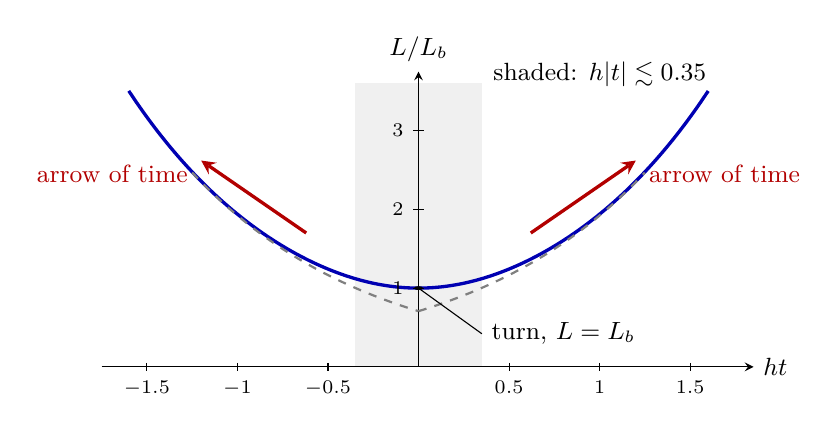
\begin{tikzpicture}[xscale=2.3,yscale=1.0,>=stealth]
  \fill[gray!12] (-0.35,0) rectangle (0.35,3.6);
  \draw[->] (-1.75,0) -- (1.85,0) node[right] {\small $ht$};
  \draw[->] (0,0) -- (0,3.75) node[above] {\small $L/\Lb$};
  \draw[very thick,blue!70!black,domain=-1.6:1.6,samples=81,smooth] plot (\x,{sqrt(cosh(2*\x))});
  \draw[dashed,gray,thick,domain=0:1.25,samples=40] plot (\x,{exp(\x)/sqrt(2)});
  \draw[dashed,gray,thick,domain=-1.25:0,samples=40] plot (\x,{exp(-\x)/sqrt(2)});
  \draw[very thick,->,red!70!black] (0.62,1.70) -- (1.20,2.62);
  \draw[very thick,->,red!70!black] (-0.62,1.70) -- (-1.20,2.62);
  \node[red!70!black,right] at (1.22,2.45) {\small arrow of time};
  \node[red!70!black,left] at (-1.22,2.45) {\small arrow of time};
  \fill (0,1) circle (0.025);
  \draw[thin] (0,1) -- (0.35,0.42);
  \node[right] at (0.35,0.42) {\small turn, $L=\Lb$};
  \node[right] at (0.36,3.72) {\small shaded: $h|t|\lesssim0.35$};
  \foreach \xx in {-1.5,-1,-0.5,0.5,1,1.5} \draw (\xx,0.05) -- (\xx,-0.05) node[below] {\scriptsize $\xx$};
  \foreach \yy in {1,2,3} \draw (0.03,\yy) -- (-0.03,\yy) node[left] {\scriptsize $\yy$};
\end{tikzpicture}
\caption{The turning solution, Eq.~\eqref{eq:rA-turning-solution}, and its two-branch reading.
The edge $L$ of the cubic torus contracts, turns at $L=\Lb$ and re-expands; dashed: the de~Sitter asymptotes $\Lb e^{h|t|}/\sqrt2$.
In the two-branch reading (assumption~\ref{assump:A4}, Sec.~\ref{rep:gate}) both halves are futures of the turning point, with arrows of time pointing away from it.
The shaded band marks the window $h|t|\lesssim0.35$ within which a real Gaussian shape state must be set for the shape to survive on both branches with probability $90\%$ (Sec.~\ref{rep:quantum-shape}).}
\label{fig:rA-turning}
\end{figure}

\subsection{Conformal time and the duration of the turn}
\label{rA:turn-duration}

The Higgs zero mode and the light fields evolve in conformal time $\eta$, $dt=L\,d\eta$, in which a light ray crosses the torus once per unit of $\eta$.
Along Eq.~\eqref{eq:rA-turning-solution}
\begin{equation}
\eta(t)=\int_0^t\frac{dt'}{L(t')}=\frac{1}{h\Lb}\int_0^{ht}\frac{d\tau}{\sqrt{\cosh2\tau}} ,
\end{equation}
which converges as $t\to\pm\infty$ because the integrand falls as $\sqrt2\,e^{-|\tau|}$.
Each branch therefore lasts a finite conformal time,
\begin{equation}
\eta_\infty=\frac{1}{h\Lb}\int_0^\infty\frac{d\tau}{(\cosh2\tau)^{1/2}}=\frac{1}{2h\Lb}\int_0^\infty{\rm sech}^{1/2}x\,dx=\frac{\Gamma(\tfrac14)^2}{4\sqrt{2\pi}\,h\Lb}=\frac{1.31103}{h\Lb},
\label{eq:rA-etainf}
\end{equation} %
where we used $\int_0^\infty{\rm sech}^\nu x\,dx=\tfrac12\sqrt\pi\,\Gamma(\tfrac\nu2)/\Gamma(\tfrac{\nu+1}2)$ at $\nu=\tfrac12$ and $\Gamma(\tfrac14)\Gamma(\tfrac34)=\sqrt2\,\pi$.
The number $1.31103$ is half the lemniscate constant, for a reason that the conformal-time form of the solution makes plain.

\paragraph{Lemniscatic form.}
In conformal time, with $a\equiv L$ and $a'=da/d\eta=La\,H$, the constraint reads $a'^2=a^4H^2=h^2(a^4-\Lb^4)$.
For $Y\equiv a^2$ this becomes $Y'^2=4h^2Y(Y^2-\Lb^4)$, a cubic in $Y$.
With $Y=\Lb^2\,\wp(z)$ and $z=h\Lb\,\eta$ it takes the Weierstrass form $\wp'^2=4\wp^3-g_2\wp-g_3$ with $g_2=4$ and $g_3=0$, the lemniscatic case:
\begin{equation}
L(\eta)^2=\Lb^2\,\wp\big(h\Lb(\eta-\eta_0);4,0\big),
\label{eq:rA-lemniscatic}
\end{equation}
with the turn at the real half period, where $\wp=e_1=1$.
The scale factor diverges at the two poles of $\wp$ that bound the real period, so the whole history spans the finite conformal interval $2\omega_1/h\Lb$, with $\omega_1=\int_1^\infty dt/\sqrt{4t^3-4t}=1.31103$, in agreement with Eq.~\eqref{eq:rA-etainf}. %
The same variables give the identity
\begin{equation}
\frac{a''}{a}=\dot a^2+a\ddot a=a^2\big(2H^2+\dot H\big)=2h^2a^2
\label{eq:rA-app}
\end{equation}
along the whole solution, by Eq.~\eqref{eq:rA-H-turn}: the turning point acts on minimally coupled fields exactly as de~Sitter space does, because the Casimir stress is traceless.
Sections~\ref{rep:gate} and~\ref{rep:spectra} use Eq.~\eqref{eq:rA-app}; with Eq.~\eqref{eq:rA-lemniscatic} it turns the mode equation of a minimally coupled field into the Lam\'e equation $d^2v/dz^2=[2\wp(z)-k^2/(h\Lb)^2]v$.

\paragraph{The duration used in the Higgs chapters.}
On the plateau the rate of the cosh solution is $\rAHeff$ rather than $h$ (Sec.~\ref{rA:turn-plateau}), so the conformal duration of one branch is $\eta_\infty=1.31103/(\rAHeff\Lb)$.
The Higgs calculation uses $\rAHeff\Lb=0.00437243$, which gives $\eta_\infty=299.84$ in units of $1/L$. %
This is the duration of the turn that enters the survival of the Higgs zero mode (Sec.~\ref{rep:h-survival}); the threshold depends on it only logarithmically (Sec.~\ref{rep:h-universality}).
The constant $\rAHeff\Lb$ of the Higgs calculation and the plateau ratio $h\Lb=0.0044$ of the benchmark differ by the factor $0.98949$ and must not be interchanged. %
Most of a branch is spent near the turn: half of $\eta_\infty$ elapses by $ht=0.76$, $64\%$ by the onset of shape freezing at $ht\simeq1.09$, and $90\%$ by $ht=2.38$, after which the integrand falls as $\sqrt2\,e^{-ht}$. %

\subsection{Null completeness and the violation of the null energy condition}
\label{rA:turn-complete}

The solution is null geodesically complete.
Along a null geodesic with conserved comoving momentum $\bm p$, the physical frequency is $\omega=|\bm p|/L$ and the affine parameter obeys $d\lambda=L\,dt/|\bm p|$.
Since $\int L\,dt=\Lb\int\sqrt{\cosh2ht}\,dt$ diverges at both ends, every null geodesic has infinite affine length in both directions.
By Corollary~3.3 of Ref.~\cite{Zhou:2026szo}, a non-static Bianchi~I spacetime that obeys the null energy condition has every null geodesic incomplete, so the Casimir state must violate that condition.
It does: $\rho+p=\tfrac43\rho_C<0$.

\subsection{The averaged null energy}
\label{rA:turn-anec}

The averaged null energy along every null geodesic quantifies the violation, and we find it in closed form.
For the isotropic leading background $R_{kk}\equiv R_{\mu\nu}k^\mu k^\nu=(\rho+p)\,\omega^2/\MPbar^2$ with $\rho+p=\tfrac43\rho_C=-\tfrac43C_{\rm eff}/L^4$, and Eq.~\eqref{eq:rA-turning-solution} gives $C_{\rm eff}/(\MPbar^2\Lb^4)=3h^2$.
With $d\lambda=dt/\omega$ and $\omega=|\bm p|/L$,
\begin{equation}
\begin{aligned}
\int R_{kk}\,d\lambda&=\frac{1}{\MPbar^2}\int(\rho+p)\,\omega\,dt=-\frac{4C_{\rm eff}|\bm p|}{3\MPbar^2}\int\frac{dt}{L^5}=-4h^2|\bm p|\Lb^4\int\frac{dt}{L^5}\\
&=-\frac{4h^2|\bm p|}{\Lb}\int_{-\infty}^{\infty}\frac{dt}{(\cosh2ht)^{5/2}}=-2h\,\omega_b\int_{-\infty}^{\infty}{\rm sech}^{5/2}x\,dx,
\end{aligned}
\label{eq:rA-anec-integral}
\end{equation}
with $\omega_b=|\bm p|/\Lb$ the null frequency at the turning point.
Since $\int{\rm sech}^{5/2}x\,dx=\sqrt\pi\,\Gamma(\tfrac54)/\Gamma(\tfrac74)$ and $\Gamma(\tfrac54)/\Gamma(\tfrac74)=\tfrac{\frac14\Gamma(\frac14)}{\frac34\Gamma(\frac34)}=\Gamma(\tfrac14)^2/(3\sqrt2\,\pi)$,
\begin{equation}
\int R_{kk}\,d\lambda=-\frac{\sqrt2\,\Gamma(1/4)^2}{3\sqrt\pi}\,h\,\omega_b=-3.4961\,h\,\omega_b . %
\label{eq:rA-anec}
\end{equation}
The result is negative for every null geodesic and proportional to its frequency at the turn.

\paragraph{The averaged sum rule.}
The violation satisfies the averaged sum rule $I_p=-J_p$ that Proposition~4.1 of Ref.~\cite{Zhou:2026szo} establishes for complete null geodesics, where $I_p=\int R_{kk}\,d\lambda$ and $J_p=\int\Tr B_p^2\,d\lambda$.
The optical tensor is $B_p=\omega H\,\rAone_2$, so $J_p=2|\bm p|\int H^2L^{-1}dt$.
On the solution this is
\begin{equation}
J_p=\frac{2|\bm p|h^2}{\Lb}\int\frac{\tanh^22ht}{(\cosh2ht)^{1/2}}\,dt=h\,\omega_b\int\big({\rm sech}^{1/2}x-{\rm sech}^{5/2}x\big)dx=2h\,\omega_b\int{\rm sech}^{5/2}x\,dx,
\end{equation}
because $\int{\rm sech}^{1/2}x\,dx=\sqrt\pi\,\Gamma(\tfrac14)/\Gamma(\tfrac34)$ is exactly three times $\int{\rm sech}^{5/2}x\,dx$.
Hence $I_p=-J_p$ holds analytically on the leading solution; numerical quadrature confirms it to $2\times10^{-16}$. %
The identity is the integrated null Raychaudhuri equation, $d(\Tr B_p)/d\lambda=-\Tr B_p^2-R_{kk}$, whose boundary term $\Tr B_p=2\omega H$ vanishes at both ends because $\omega\to0$.

\paragraph{Achronal averaged null energy condition.}
Every null geodesic of the torus winds around it and is not achronal, so this violation is consistent with the achronal averaged null energy condition, the version free of known violations by quantum fields~\cite{Graham:2007va}.

\subsection{The plateau turning point and its calibration}
\label{rA:turn-plateau}

For the plateau of Eq.~\eqref{eq:rA-plateau} the turning point sits at an inflaton value $\phi_b$ with $H=\dot\phi=0$, and the history is time symmetric.
At the turn the vacuum energy is $V(\phi_b)$, which replaces $h$ in Eq.~\eqref{eq:rA-turning-solution} by
\begin{equation}
\rAHeff=\frac{1}{\MPbar}\Big[\frac{V(\phi_b)}{3}\Big]^{1/2}=\big(1-e^{-\sqrt{2/3}\,\phi_b/\MPbar}\big)\,h=0.9895\,h ;
\label{eq:rA-Heff}
\end{equation} %
the numbers below include this factor.
Elsewhere we measure time in units of $1/h$, $\tau\equiv ht$, because the $1\%$ difference is below the accuracy of every result that uses Eq.~\eqref{eq:rA-turning-solution}, except the shape thresholds of Sec.~\ref{rep:quantum-shape}, which are in units of $1/\rAHeff$.

\paragraph{Calibration.}
We fix $h$ by the observed scalar amplitude and the pivot $k_*=0.05\,{\rm Mpc}^{-1}$ by thermal matching. %
With instant reheating this gives $N_*=55.722$ e-folds between pivot exit and the end of inflation and $h/\MPbar=6.116\times10^{-6}$ (Sec.~\ref{rep:spectra}). %
For the AAA Standard Model with free fields and a reference present torus side $L_0=6/H_0$, $0.96$ times the diameter $\dLSS$ of the last-scattering sphere, a pivot solver gives $\phi_b=5.5794\,\MPbar$, $N_{\rm post}=68.25$ e-folds after the turning point and $h\Lb=0.00483$. %
The solver integrates the background from the turn with the inflaton released at $\phi_b$, finds the end of inflation and the e-fold at which $k_*$ leaves the Hubble radius, and adjusts $\phi_b$ so that the comoving torus scale today is $L_0$.
The present size enters only through $\ln L_0$: for $0.95\leq L_0/\dLSS\leq2$ the turning-point quantities $V(\phi_b)$ and $h\Lb$ change by at most $2.2\times10^{-4}$, while $N_{\rm post}$ grows by $\ln(L_0H_0/6)$. %

\paragraph{The benchmark.}
With free fields Eq.~\eqref{eq:rA-turning-solution} gives $(\Lb\MPbar)^4=\NC\rAgam/[3(\rAHeff/\MPbar)^2]$, that is $\Lb\MPbar=790$. %
The zero-mode energy replaces $\NC$ by $\rANeff$ in Eq.~\eqref{eq:rA-turning-solution}, which lowers $\Lb$ by the factor $(1-\fzm)^{1/4}=0.9147$, or $8.5\%$. %
The benchmark turning point therefore has
\begin{equation}
\Lb\MPbar=722,\qquad h\Lb=0.0044, %
\label{eq:rA-benchmark}
\end{equation}
and the matching scale of assumption~\ref{assump:A2} is $\mub=1/\Lb=\MPbar/722=3.37\times10^{15}$\,GeV. %
At fixed $L_0$ the factor $0.9147$ acts like a change of $\ln L_0$ by $0.09$, so $V(\phi_b)$ changes by less than $10^{-4}$ and $N_{\rm post}$ grows by $0.09$. %
Table~\ref{tab:rA-fzero} collects the background quantities with and without the zero-mode energy.

\begin{table}[tbp]
\centering
\caption{Background quantities for free fields ($\fzm=0$) and with the leading-order zero-mode energy ($\fzm=0.30$, the benchmark). %
$\rANeff=(1-\fzm)\NC$; $\Lb$ and $h\Lb$ refer to the plateau history of this chapter; $\kappa_E$ and $\kappa_{T_2}$ are the normalized stiffnesses of the aspect and angle modes at the cube (Sec.~\ref{rep:shape}).
The first next-order corrections lower $\fzm$ to $0.28$ and $\kappa_E$ to $18.0$ ($\kappa_{T_2}=-8.34$).} %
\label{tab:rA-fzero}
\begin{tabular}{lcc}
\toprule
 & $\fzm=0$ & $\fzm=0.30$\\ %
\midrule
$\rANeff$ & $25.5$ & $17.9$\\ %
$\Lb\MPbar$ & $790$ & $722$\\ %
$h\Lb$ & $0.0048$ & $0.0044$\\ %
$\kappa_E$; $\kappa_{T_2}$ & $13.53$; $-6.35$ & $19.32$; $-9.07$\\ %
\bottomrule
\end{tabular}
\end{table}

\subsection{Scales of the turning point}
\label{rA:turn-scales}

The benchmark torus is $\Lb=722\sqrt{8\pi}\,\ell_{\rm P}\simeq3.6\times10^3$ Planck lengths, or $6\times10^{-32}$\,m, across, about $230$ times smaller than the Hubble radius $1/h$. %
The small parameter of the semiclassical description is
\begin{equation}
\epsilon=\sqrt{\NC}\,\frac{h}{\MPbar}=\sqrt{\frac{3}{\rAgam}}\,(h\Lb)^2\simeq3\times10^{-5},
\label{eq:rA-epsilon}
\end{equation} %
where the second form, with the free-field $\Lb$ and the rate of the cosh solution in place of $h$, follows from $(\rAHeff\Lb)^4=\NC\rAgam\rAHeff^2/3\MPbar^2$; the two forms differ by the $1\%$ between $h$ and $\rAHeff$.
It is the squared ratio of the light-crossing time of the torus to the Hubble time at the turn, up to the factor $\sqrt{3/\rAgam}=1.338$, the factor with which the finite-volume shape inertia of Sec.~\ref{rep:shape} enters.
Anomalous corrections to the criterion~\eqref{eq:rA-exact-criterion} are of relative order $\epsilon^2$.
The turning point is also slow compared with the photon gap: the lowest photon pair has the frequency $4\pi/\Lb$, and the adiabaticity parameter of the turn is $(h\Lb/4\pi)^2\simeq1.2\times10^{-7}$, so the lowest photon modes follow it adiabatically (Sec.~\ref{rep:gate}). %
All modes of the torus are inside the Hubble radius at the turn by at least the factor $2\pi/(h\Lb)\simeq1400$ (1300 for free fields; Sec.~\ref{rep:spectra}). %

\section{Higgs zero mode I: finite-volume matching}\label{rep:h-matching}

At the turning point the torus has edge $\Lb=722\,\MPbar^{-1}$ (Sec.~\ref{rep:turning}), so the couplings that act on its zero modes are the Standard Model couplings at $\mub=1/\Lb=\MPbar/722=3.37\times10^{15}\GeV$. %
This section derives, from the Standard Model Lagrangian, the quantum mechanics of the electroweak zero modes and the one-loop energy that the non-zero modes add to it.
We show four things.
(i)~The constant modes of the Higgs doublet and of the SU(2)$\times$U(1)$_Y$ gauge fields form a system with sixteen coordinates, whose gauge zero-point motion confines the Higgs radius linearly.
(ii)~The one-loop energy of a tower of non-zero modes, summed in finite volume and renormalized in $\MSbar$, is analytic in the field-dependent squared mass below the first non-zero momentum, tachyonic masses included; its leading term is a negative tadpole for periodic bosons.
(iii)~With the Coulomb-gauge Higgs zero mode as the slow coordinate, every massive vector contributes two transverse modes and one Coulomb mode, and the explicit scale dependence of the one-loop energy cancels the running of the couplings if and only if the Higgs field carries the Coulomb-gauge anomalous dimension; the covariant Landau-gauge counting agrees with this split to $0.016\GeV$ in the critical top mass, whereas the gauge-invariant (unitary) counting is not consistent. %
(iv)~In the sector of order $r^2c^2$, where $c$ is a gauge holonomy, the transverse vev mixing, the instantaneous Coulomb mismatch, and the exact top chiral loop close the renormalization-group equation of the tree-level gauge--Higgs term to $97$--$99\%$, so $\mu=1/L$ is a consistent matching scale for all one-loop terms. %
The last subsection gives the matching-scale scan of the final model, which is the matching item of the error budget (Sec.~\ref{rep:h-budget}).
Figure~\ref{fig:rb-diagrams} shows the one-loop diagrams that enter.

Throughout Secs.~\ref{rep:h-matching}--\ref{rep:h-universality} we use units $L=1$, in which fields and energies are measured in $1/L$, and $\MSbar$ couplings.
Four configurations recur.
\emph{Fixed-coupling} calculations use the one-loop couplings at $1/\Lb$ of Sec.~\ref{rep:zeromodes}, $g_2=0.5268$, $g_3=0.5396$, $g_Y=0.4415$, and $y_t=0.4585$, without running. %
The \emph{earlier Standard Model mapping} is two-loop running with fitted matching and a constant three-loop calibration of $\lambda$; the NNLO mapping of Sec.~\ref{rep:h-smmap} replaces it.
The \emph{final model} is the node-direct two-dimensional model of Sec.~\ref{rep:h-reduced} with the NNLO mapping and all cross terms of Sec.~\ref{rep:h-cross}; the \emph{earlier model} is the same model before the last one-loop cross terms of Sec.~\ref{sec:rb-r2c2}.
All statements hold under assumptions (A1)--(A7) of Sec.~\ref{rep:setup}; we name the assumption where it enters.

\subsection{The electroweak zero-mode Hamiltonian}
\label{sec:rb-H0}

We expand every field on the torus in Fourier modes $\bm k=2\pi(\bm n+\bm\theta)$, $\bm n\in\mathbb Z^3$, with $\bm\theta=0$ for periodic and $\bm\theta=(\frac12,\frac12,\frac12)$ for antiperiodic fields (AAA spin structure, assumption (A1)).
The constant modes of the bosons are slow coordinates of finite-dimensional quantum mechanics; all other modes are fast and are integrated out at one loop in Secs.~\ref{sec:rb-tower}--\ref{sec:rb-r2c2}.
In temporal gauge $A_0=0$ the constant modes are the Higgs doublet
\begin{equation}
\Phi=\frac{1}{\sqrt2}\begin{pmatrix}\phi_0+i\phi_1\\ \phi_2+i\phi_3\end{pmatrix},\qquad r\equiv|\bm\phi|,\qquad \Phi^\dagger\Phi=\frac{r^2}{2},
\label{eq:rb-Phi}
\end{equation}
the SU(2) connection $\bm x_i=(x_i^1,x_i^2,x_i^3)$ and the hypercharge connection $w_i$, $i=1,2,3$.
With the normalization $\mathcal L\supset-\frac14F^a_{\mu\nu}F^{a\mu\nu}$ and $D_\mu=\partial_\mu-ig_2A_\mu^aT^a-ig_YYB_\mu$, the constant modes $A_i^a=x_i^a$ and $B_i=w_i$ have unit kinetic terms, and the holonomy angles that twist charged fields are $c_i=g_2\bm x_i\cdot\bm T$ and $u_i=g_Yw_i$ (in units $1/L$).
For constant fields the field strength reduces to its commutator part, $F_{ij}^a=g_2\,\epsilon^{abc}x_i^bx_j^c=g_2(\bm x_i\times\bm x_j)^a$, and the covariant derivative of a constant doublet to $D_i\Phi=-i(g_2\bm x_i\cdot\bm T+g_YYw_i)\Phi$.
The Hamiltonian of the zero modes is therefore~\cite{Luscher:1982ma,Koller:1987fq,vanBaal:2000zc}
\begin{align}
H_0={}&\tfrac12 p_x^2+\tfrac12 p_w^2+\tfrac12 p_\phi^2+\frac{g_2^2}{4}\sum_{i,j}|\bm{x}_i\times\bm{x}_j|^2 \nonumber\\
&+\sum_i\Phi^\dagger\bigl(g_2\,\bm{x}_i\cdot\bm{T}+g_Y Y w_i\bigr)^2\Phi+\frac{\lambda}{4}r^4,
\label{eq:rb-H0}
\end{align}
with $\bm T=\bm\sigma/2$, $Y=\frac12$, and the $\MSbar$ couplings $g_2$, $g_Y$, and $\lambda$ at $\mu=1/L$.
The four terms are the electric energy of the constant connections, the magnetic energy $\frac14\sum_{ij}F_{ij}^aF_{ij}^a$, the gradient energy $\sum_i|D_i\Phi|^2$ of the constant doublet, and the quartic potential; the Higgs mass parameter is negligible at $\mu\sim10^{15}\GeV$.
The gluon zero modes do not couple to $\Phi$ at tree level; they enter through the top-quark loop of Sec.~\ref{rep:h-cross}.
Equation~(\ref{eq:rb-H0}) has sixteen coordinates: nine SU(2), three hypercharge, and four Higgs components.

The zero mode of $A_0$ is a Lagrange multiplier whose equation is Gauss's law: physical states are invariant under constant SU(2)$\times$U(1)$_Y$ transformations, which act orthogonally on $(\bm x,\bm w,\bm\phi)$.
We fix this freedom by rotating the unit vector $\bm N=2\Phi^\dagger\bm\sigma\Phi/r^2$ to $\bm e_3$, which puts the vev in the upper component, $\Phi=(r/\sqrt2)(1,0)^{\mathsf T}$, and leaves U(1)$_{\rm em}$ generated by $T^3-Y$ acting on the doublet.
In four dimensions the Laplacian of $\bm\phi$ is $r^{-3}\partial_rr^3\partial_r+r^{-2}\Delta_{S^3}$, and on gauge-invariant states the angular part acts through the SU(2) rotations of $\bm x$, so that
\begin{equation}
H_0=-\frac{1}{2r^3}\partial_r r^3\partial_r+\frac{2}{r^2}\bigl[(L^1)^2+(L^2)^2\bigr]+H_{\rm g}(\bm{x},\bm{w};r),
\label{eq:rb-bodyframe}
\end{equation}
where $L^a$ generates SU(2) rotations of $\bm x$ and $H_{\rm g}$ contains the kinetic, magnetic, and mass terms of the gauge zero modes~\cite{Luscher:1982ma,vanBaal:2000zc}.
The radial operator is self-adjoint with the flat measure $r^3dr$; with $f=r^{-3/2}u$ one finds
\begin{equation}
-\frac{1}{2}\Bigl(f''+\frac{3}{r}f'\Bigr)=r^{-3/2}\Bigl[-\frac12u''+\frac{3}{8r^2}u\Bigr],
\label{eq:rb-centrifugal}
\end{equation}
which is the origin of the term $3/(8r^2)$ in the reduced models of Sec.~\ref{rep:h-reduced}; regular states behave as $u\propto r^{3/2}$.

In the body frame the gradient term of Eq.~(\ref{eq:rb-H0}) becomes a mass term for the gauge zero modes.
With $\Phi=(r/\sqrt2)(1,0)^{\mathsf T}$ and $M_i=g_2\bm x_i\cdot\bm T+g_YYw_i$,
\begin{equation}
\Phi^\dagger M_i^2\Phi=\frac{r^2}{8}\Bigl[g_2^2\bigl((x_i^1)^2+(x_i^2)^2\bigr)+\bigl(g_2x_i^3+g_Yw_i\bigr)^2\Bigr]\equiv\tfrac12\,y_i^{\mathsf T}\mathcal M y_i,
\label{eq:rb-massterm}
\end{equation}
where $y_i=(x_i^1,x_i^2,x_i^3,w_i)$ and, in each spatial direction,
\begin{equation}
\mathcal M=\frac{r^2}{4}\,{\rm diag}\bigl(g_2^2,\,g_2^2,\,\mathcal M_2\bigr),\qquad
\mathcal M_2=\begin{pmatrix}g_2^2&g_2g_Y\\ g_2g_Y&g_Y^2\end{pmatrix}.
\label{eq:rb-massmatrix}
\end{equation}
Its eigenvalues describe two $W$ modes of frequency $g_2r/2$, a $Z$ mode of frequency $g_Zr/2$ with $g_Z=(g_2^2+g_Y^2)^{1/2}$, and a massless photon $\propto g_Yx_i^3-g_2w_i$.

The confinement of the Higgs radius follows from this mass matrix.
For $r\gtrsim1$ the $W$ and $Z$ zero modes are nearly harmonic, and since each of the three spatial directions carries two $W$ modes and one $Z$ mode, their zero-point energy is
\begin{equation}
E_{\rm g}(r)\simeq E_{\rm g}^{(0)}+3\Bigl[2\cdot\frac12\,\frac{g_2r}{2}+\frac12\,\frac{g_Zr}{2}\Bigr]=E_{\rm g}^{(0)}+\sigma_0 r,\qquad \sigma_0=\tfrac32 g_2+\tfrac34 g_Z\simeq1.31. %
\label{eq:rb-linear}
\end{equation}
At smaller $r$ the magnetic quartic term of Eq.~(\ref{eq:rb-H0}) dominates, the gauge ground state is anharmonic, and its energy scales as $g^{2/3}$~\cite{Luscher:1982ma,Koller:1987fq}.
With $\lambda<0$ a radial potential of the form $\sigma r-|\lambda|r^4/4$ has a well near the origin, a barrier at $r_{\rm top}=(\sigma/|\lambda|)^{1/3}$, and a runaway beyond it, so the electroweak configuration is a resonance (Sec.~\ref{rep:h-reduced}).
The negative quartic leaves the zero-mode share $\fzm$ of Sec.~\ref{rep:zeromodes}, and hence the turning solution, unchanged at the quoted precision.

\subsection{Non-zero modes in the zero-mode background}
\label{sec:rb-masses}

The non-zero modes see the zero modes as a constant background.
Expanding the Standard Model Lagrangian to second order in the fluctuations around $\Phi=(r/\sqrt2)(1,0)^{\mathsf T}$ with trivial holonomy gives the field-dependent squared masses
\begin{align}
&a_W=\frac{g_2^2r^2}{4},\qquad a_Z=\frac{g_Z^2r^2}{4},\qquad b=\frac{V_{\rm tree}'(r)}{r}=\lambda r^2,\nonumber\\
&m_{\delta\rho}^2=V_{\rm tree}''(r)=3\lambda r^2,\qquad \tilde m_t^2=\frac{y_t^2r^2}{2},
\label{eq:rb-masses}
\end{align}
for the $W$ and $Z$ bosons, the three Goldstone modes (off shell, since $V'_{\rm tree}=\lambda r^3\neq0$), the radial fluctuation $\delta\rho$, and the top quark, with $V_{\rm tree}=\lambda r^4/4$.
For $\lambda<0$ both $b$ and $m_{\delta\rho}^2$ are negative.
A tachyonic mass in finite volume is harmless as long as every frequency $\omega_k^2=k^2+m^2$ stays positive, i.e., $|m^2|<(2\pi)^2$ for periodic and $|m^2|<3\pi^2$ for antiperiodic fields.
In the field range of the resonance all masses are small on this scale: for $r\le5$, $m_Z\le1.72/L$ and $\tilde m_t\le1.51/L$, at least $3.6$ times below $2\pi/L$, and the radial non-zero modes become tachyonic only at $r\approx31$, far outside the barrier at $r\approx4$--$5$. %

\subsection{One tower of non-zero modes: \texorpdfstring{$\MSbar$}{MS-bar} finite-volume sum}
\label{sec:rb-tower}

For one real degree of freedom of squared mass $m^2$ the non-zero modes have energy $\frac12\sum_{\bm k}'\omega_k$, $\omega_k^2=k^2+m^2$, where the prime removes $\bm k=0$ for periodic fields.
We write it as the infinite-volume integral, which we regularize dimensionally, plus the convergent difference between sum and integral.
The difference follows from the proper-time identity
\begin{equation}
A^{1/2}=-\frac{1}{2\sqrt\pi}\int_0^\infty\frac{ds}{s^{3/2}}\bigl(e^{-As}-1\bigr),\qquad A>0,
\label{eq:rb-propertime}
\end{equation}
applied to each mode, with the heat-kernel sum $K_\theta(s)=\sum_{\bm n}e^{-4\pi^2|\bm n+\bm\theta|^2s}$ and its continuum limit $(4\pi s)^{-3/2}=\int d^3k\,(2\pi)^{-3}e^{-k^2s}$.
Removing also the value at $m^2=0$, which is part of the Casimir energy of Sec.~\ref{rep:casimir}, we obtain
\begin{equation}
D_\theta(m^2)=-\frac{1}{4\sqrt\pi}\int_0^\infty\!\frac{ds}{s^{3/2}}\bigl(e^{-m^2s}-1\bigr)\Bigl[K_\theta(s)-\delta_{\theta0}-(4\pi s)^{-3/2}\Bigr],
\label{eq:rb-Dtheta}
\end{equation}
where $\delta_{\theta0}$ removes the $\bm k=0$ term of periodic fields.
The integral converges at both ends: at small $s$ the Poisson form $K_\theta(s)-(4\pi s)^{-3/2}=(4\pi s)^{-3/2}\sum_{\bm n\neq0}e^{-n^2/4s}\cos(2\pi\bm n\cdot\bm\theta)$ is exponentially small, and at large $s$ the bracket tends to $-(4\pi s)^{-3/2}$.
In $d=3-2\epsilon$ spatial dimensions the integral gives, after $\MSbar$ subtraction, the Coleman--Weinberg term~\cite{Coleman:1973jx}
\begin{equation}
V_{\rm CW}(m^2;c,\mu)=\frac{m^4}{64\pi^2}\Bigl[\ln\frac{|m^2|}{\mu^2}-c\Bigr],\qquad c=\tfrac32\ \text{for a scalar},
\label{eq:rb-VCW}
\end{equation}
with the tree-level couplings taken at the same $\mu$.
The one-loop energy of the tower is therefore
\begin{equation}
E_{\rm std}(m^2;\mu)=D_\theta(m^2)+V_{\rm CW}(m^2;\tfrac32,\mu).
\label{eq:rb-Estd-def}
\end{equation}

\paragraph{Analyticity.}
The logarithms cancel.
For $|m|$ below the smallest non-zero momentum, $2\pi$ for periodic and $\sqrt3\,\pi$ for antiperiodic fields, each term $(k^2+m^2)^{1/2}=k\sum_j\binom{1/2}{j}(m^2/k^2)^j$ has a convergent binomial series.
The lattice sums of the terms of order $k$, $k^{-1}$, and $k^{-3}$ diverge; after regularization they are polynomials of order $m^0$, $m^2$, and $m^4$, and the pole of the last one is removed by the $\MSbar$ counterterm, which leaves $\ln\mu$.
All other terms converge absolutely, so the regularized sum is analytic in $m^2$.
The continuum integral contains the non-analytic term $+m^4\ln|m^2|/(64\pi^2)$, so $D_\theta$ contains its negative, and
\begin{equation}
E_{\rm std}=\frac{T_\theta}{2}\,m^2+\Bigl[c_2-\frac{\ln\mu^2L^2+\frac32}{64\pi^2}\Bigr]m^4+O(m^6),
\label{eq:rb-Estd}
\end{equation}
with $c_2=0.0062594$ for periodic fields, is analytic for $|m|<2\pi/L$ (periodic) or $|m|<\sqrt3\,\pi/L$ (antiperiodic). %
A tachyonic mass, such as $m_{\delta\rho}^2$ or the Goldstone mass $b$ for $\lambda<0$, therefore needs no prescription, and $E_{\rm std}$ is smooth through $m^2=0$.
Numerically the coefficient of $m^4\ln|m^2|$ in $D_P$ is $-0.00158314349=-1/(64\pi^2)$ on both sides of $m^2=0$ to $10^{-9}$, and the Cauchy--Riemann residual of the continued function is $10^{-11}$. %

\paragraph{Tadpole.}
The coefficient of $m^2$ is the finite-volume tadpole, the regularized $\frac14\sum_{\bm k}'1/k$.
In Eq.~(\ref{eq:rb-Dtheta}) the term $-\delta_{\theta0}$ integrates to $-m/2$ exactly, and the large-$|\bm n|$ part of the Poisson sum returns $+m/2$, so the two non-analytic pieces cancel.
The remaining first-order term, with the lattice sum understood as its analytic continuation, is
\begin{equation}
\frac{T_\theta}{2}=\frac{1}{4\sqrt\pi}\int_0^\infty\!\frac{ds}{s^{1/2}}\,(4\pi s)^{-3/2}\sum_{\bm n\neq0}e^{-n^2/4s}\cos(2\pi\bm n\cdot\bm\theta)
=\frac{1}{8\pi^2}\sum_{\bm n\neq0}\frac{\cos(2\pi\bm n\cdot\bm\theta)}{|\bm n|^2}\equiv\frac{Z_1}{8\pi^2},
\label{eq:rb-tadpole}
\end{equation}
where the periodic sum is the analytically continued Epstein constant, $Z_P=-8.913633$, and the antiperiodic one, with $\cos(2\pi\bm n\cdot\bm\theta)=(-1)^{n_1+n_2+n_3}$, is $Z_A=-2.519356$. %
Hence $T_B/2=Z_P/(8\pi^2)=-0.1128925$ and $T_F/2=Z_A/(8\pi^2)=-0.0319080$. %
Both are negative: the non-zero modes have less zero-point energy in a box than in the continuum, and a mass lowers their energy further.
The tadpole of the periodic bosons is the term that matters most below.

\paragraph{Why the non-zero modes undo part of the zero-point confinement.}
The full periodic tower, including $\bm k=0$, reproduces the continuum up to terms of order $e^{-mL}$.
Its zero mode contributes the harmonic zero-point energy $m/2$, so the non-zero modes satisfy $D_P(m^2)\to-m/2+0.8375$ for $mL\gg2\pi$, where the constant is minus the massless Casimir energy $-\frac{1}{2\pi^2}\sum_{\bm n\neq0}|\bm n|^{-4}$ removed in Eq.~(\ref{eq:rb-Dtheta}). %
In a large box the non-zero modes thus cancel the zero-point energy that confines the zero mode, as they must, since the constant mode is then not special.
At the masses of the resonance, $mL\le1.72$, the cancellation is partial and is described by the convergent series of Eq.~(\ref{eq:rb-Estd}), whose leading term is the negative tadpole. %
For the $W$ and $Z$ towers it gives $3\cdot\frac{T_B}{2}(2a_W+a_Z)=-0.087\,r^2$ at the fixed couplings, a negative mass term for the Higgs zero mode that weakens the linear confinement of Eq.~(\ref{eq:rb-linear}). %
The full one-loop matching, which also contains the stabilizing tadpole of the antiperiodic top tower (Sec.~\ref{sec:rb-rg}), lowers the local slope by $10$--$33\%$ at $r=1$--5 and roughly halves the barrier above the resonance level (Sec.~\ref{sec:rb-size}). %
Without the non-zero modes the threshold would lie at more negative $\lambda$, and at the central inputs the zero mode would survive almost surely ($\Pone\approx0.998$ in a one-dimensional version of the model); the matching is what makes the outcome depend on the top-quark mass. %

\paragraph{Numerical evaluation.}
We evaluate $D_\theta$ by splitting the proper-time integral at $s_c=0.1$. %
For $s<s_c$ the Poisson image sum makes $K_\theta(s)-(4\pi s)^{-3/2}$ exponentially small, and the zero-mode subtraction integrates in closed form,
\begin{equation}
\int_0^{s_c}\!\frac{ds}{s^{3/2}}\bigl(e^{-m^2s}-1\bigr)=-\frac{2\bigl(e^{-m^2s_c}-1\bigr)}{\sqrt{s_c}}-2\sqrt\pi\,m\,{\rm erf}\bigl(m\sqrt{s_c}\bigr),
\label{eq:rb-small-s}
\end{equation}
an entire function of $m^2$.
For $s>s_c$ each lattice shell with $\alpha=k^2+m^2$ contributes
\begin{equation}
\int_{s_c}^\infty\!\frac{ds}{s^{3/2}}\,e^{-\alpha s}=e^{-\alpha s_c}\Bigl[\frac{2}{\sqrt{s_c}}-2\sqrt{\pi\alpha}\;{\rm erfcx}\bigl(\sqrt{\alpha s_c}\bigr)\Bigr],
\label{eq:rb-shell}
\end{equation}
and the continuum term is $m^4\Gamma(-2,m^2s_c)$, continued to $m^2<0$ with $\ln z\to\ln|z|$.
As checks, $D_P/m^2\to-0.1128922$ at $m^2=10^{-5}$ against $T_B/2=-0.1128925$, and $D_A/m^2\to-0.0319078$ against $T_F/2=-0.0319080$. %
The Bessel image sum
\begin{equation}
E_{\vartheta}(m)=-\frac{m^2}{4\pi^2}\sum_{\bm n\neq0}\frac{K_2(m|\bm n|)\cos(2\pi\bm n\cdot\bm\vartheta)}{|\bm n|^2},
\label{eq:rb-Etheta}
\end{equation}
which is the complete finite-volume energy of the tower relative to the continuum (with an extra $(-1)^{n_1+n_2+n_3}$ for antiperiodic fields), agrees with $D_P$ to $5\times10^{-11}$ and with $D_A$ to $10^{-15}$ once the zero mode is restored. %
The same image sum with a twist $\bm\vartheta$ is the basis of the cross terms of Sec.~\ref{rep:h-cross}.

\paragraph{The natural scale.}
With $c_2=0.0062594$ the $m^4$ coefficient of Eq.~(\ref{eq:rb-Estd}) vanishes at %
\begin{equation}
\mu_*L=\exp\Bigl[\frac{64\pi^2c_2-\frac32}{2}\Bigr]=3.41. %
\label{eq:rb-mustar}
\end{equation}
At this scale the finite-volume energy is as close as possible to its tadpole term.
Evaluating the matching at $\mu_*$ instead of at $\mu=1/L$ lowers $m_c(\Pone=1/2)$ by $0.02$--$0.03\GeV$, inside the matching item of Sec.~\ref{sec:rb-scale}. %

\subsection{Massive vectors in Coulomb gauge}
\label{sec:rb-coulomb}

In the body frame with trivial holonomy, $W^{1,2}$ pair with the Goldstone modes $\pi^{1,2}$ at $a_W$, and $Z$ pairs with $\pi^3$ at $a_Z$.
The photon does not mix with $\pi^3$, because the neutral Gauss law is diagonal in the $(Z,\gamma)$ basis.
All three Goldstone modes have the off-shell mass $b=\lambda r^2$.
We derive the spectrum of one vector of mass $m_V^2=a$ with its Goldstone mode $\pi$ in Coulomb gauge, $\nabla\cdot\bm A=0$.

The quadratic Lagrangian of an abelianized pair follows from $|D_\mu\Phi|^2$ with $\Phi\to(r+\delta\rho+i\pi)/\sqrt2$, which contains $\frac12(\partial_\mu\pi-m_VA_\mu)^2$, from $-\frac14F^2=\frac12(\bm E^2-\bm B^2)$ with $\bm E=-\nabla A_0-\dot{\bm A}$, and from the potential $-\frac12b\pi^2$.
In Coulomb gauge the longitudinal electric field is $-\nabla A_0$, and the cross term $\bm A\cdot\nabla\pi$ integrates to zero.
In Fourier space the longitudinal sector is therefore
\begin{equation}
\mathcal L=\tfrac12k^2A_0^2+\tfrac12\bigl(\dot\pi-m_VA_0\bigr)^2-\tfrac12(k^2+b)\pi^2 ,
\label{eq:rb-coulomb-L}
\end{equation}
and the transverse sector is two modes with $\omega^2=k^2+a$.
$A_0$ has no time derivative; Gauss's law, $\partial\mathcal L/\partial A_0=0$, gives
\begin{equation}
k^2A_0=m_V\bigl(\dot\pi-m_VA_0\bigr)\quad\Longrightarrow\quad A_0=\frac{m_V\,\dot\pi}{k^2+a},\qquad \dot\pi-m_VA_0=\frac{k^2}{k^2+a}\,\dot\pi .
\label{eq:rb-gauss}
\end{equation}
Substituting back,
\begin{equation}
\mathcal L_{\rm eff}=\tfrac12 Z_k\dot\pi^2-\tfrac12(k^2+b)\pi^2,\qquad Z_k=\frac{k^2}{k^2+a},\qquad
\omega_C^2=\frac{(k^2+b)(k^2+a)}{k^2}.
\label{eq:rb-coulomb}
\end{equation}
On shell, $b=0$, the Coulomb frequency coincides with the transverse one, and the matching reduces pointwise, to $1.8\times10^{-14}$, to three polarizations of mass $a$ with $V_{\rm CW}$ included. %
The Coulomb mode is the physical longitudinal mode of the vector, dressed by the off-shell Goldstone mass.

\paragraph{$\MSbar$ constants of a massive vector.}
The constants follow from the polarization count in $d=3-2\epsilon$ dimensions.
A massive vector has $2-2\epsilon$ transverse polarizations and one longitudinal polarization.
The dimensionally regularized integral per polarization is $\frac{m^4}{64\pi^2}[-\frac1\epsilon+\ln\frac{m^2}{\mu^2}-\frac32]$ in $\MSbar$ conventions, and the $O(\epsilon)$ part of the transverse multiplicity multiplies the pole,
\begin{equation}
(2-2\epsilon)\Bigl[-\frac1\epsilon+\ln\frac{a}{\mu^2}-\frac32\Bigr]\ \xrightarrow{\ \MSbar\ }\ 2\Bigl[\ln\frac{a}{\mu^2}-\frac12\Bigr],
\label{eq:rb-polcount}
\end{equation}
so the constant of each transverse mode moves from $\frac32$ to $\frac12$ and $2(\ln-\frac12)+(\ln-\frac32)=3(\ln-\frac56)$, the usual $\MSbar$ vector constant.
Using $\frac32$ for all three polarizations mixes schemes; in the one-dimensional matching study with the earlier mapping it would have shifted $m_c$ by $-0.052\GeV$, and it is not an uncertainty. %

\paragraph{Ultraviolet subtraction of the Coulomb mode.}
The Coulomb frequency is not a relativistic dispersion, so we subtract its ultraviolet behavior with standard scalars.
Writing $\omega_C=k(1+x+y)^{1/2}$ with $x=(a+b)/k^2$ and $y=ab/k^4$ and expanding,
\begin{equation}
\omega_C=k+\frac{a+b}{2k}-\frac{(a-b)^2}{8k^3}+\frac{(a+b)(a-b)^2}{16k^5}+O(k^{-7}).
\label{eq:rb-omegaC}
\end{equation}
Three scalars of squared masses $\mu_j^2=(b,a,2a)$ with weights $c_j=(1,2b/a,-b/a)$ reproduce the terms of order $k$, $k^{-1}$, and $k^{-3}$ of $\omega_C-\omega_a$, because
\begin{equation}
\sum_jc_j=1+\frac ba,\qquad \sum_jc_j\mu_j^2=b,\qquad \sum_jc_j\mu_j^4=b^2-2ab,
\label{eq:rb-weights}
\end{equation}
and $\omega_C-\omega_a=\frac{b}{2k}+\frac{2ab-b^2}{8k^3}+\dots$.
The Coulomb mode then contributes $E_{\rm std}(a)+\Delta(a,b)$, with
\begin{align}
\Delta(a,b)={}&R(a,b)+E_{\rm std}(b)+\frac{2b}{a}E_{\rm std}(a)-\frac{b}{a}E_{\rm std}(2a),\nonumber\\
R(a,b)={}&\tfrac12\sum_{\bm k}{}'\Bigl[\omega_C-\omega_a-\omega_b-\frac{2b}{a}\omega_a+\frac{b}{a}\omega_{2a}+\Bigl(1+\frac ba\Bigr)k\Bigr].
\label{eq:rb-Delta}
\end{align}
The summand of $R$ falls as $(5a^2b-ab^2)/(32k^5)$, which follows from the $k^{-5}$ terms of Eq.~(\ref{eq:rb-omegaC}) and of the scalars, so we sum shells with $|\bm n|\le60$ and add the tail analytically. %
Because each $E_{\rm std}$ is the exact $\MSbar$ finite-volume energy, $\Delta$ does not depend on the subtraction: replacing $2a$ by $1.5a$ or $3a$ changes it by at most $5\times10^{-9}$. %
Its scale dependence follows from Eq.~(\ref{eq:rb-weights}),
\begin{equation}
\frac{d\Delta}{d\ln\mu^2}=-\frac{1}{64\pi^2}\sum_jc_j\mu_j^4=-\frac{b^2-2ab}{64\pi^2},
\label{eq:rb-Delta-mu}
\end{equation}
which the numerics reproduce to $10^{-15}$. %

The Goldstone mass enters only through $\Delta(a,b)$.
Its first-order part is $\partial_b\Delta|_{b=0}=\frac12\langle\pi^2\rangle_{\rm FV}$, the finite-volume fluctuation with Coulomb weight $(k^2+a)^{1/2}/(2k^2)$, which tends to $T_B/2$ as $a\to0$. %
Keeping only this term moves $m_c$ by $-0.0005$ and $-0.0009\GeV$ at $\Pone=0.9$ and $1/2$ and $\Gamma(\lambda=-0.010)$ by $0.3\%$, so the exact treatment matters little; we keep it. %

\subsection{The one-loop matching potential}
\label{sec:rb-dVMC}

Summing two transverse modes and the Coulomb mode for each of $W$, $W$, and $Z$, and adding the radial mode and the top quark, gives the one-loop matching potential
\begin{align}
\Delta V_{\rm MC}(r)={}&\sum_{V=W,W,Z}\Bigl[3D_P(a_V)+2V_{\rm CW}(a_V;\tfrac12)+V_{\rm CW}(a_V;\tfrac32)+\Delta(a_V,b)\Bigr]\nonumber\\
&+E_{\rm std}(3\lambda r^2)-12\bigl[D_A(\tilde m_t^2)+V_{\rm CW}(\tilde m_t^2;\tfrac32)\bigr],
\label{eq:rb-dVMC}
\end{align}
where $D_P$ and $D_A$ are $D_\theta$ for periodic and antiperiodic fields.
The top quark has $4\times3=12$ real degrees of freedom per Dirac field and color sum, antiperiodic boundary conditions, and the fermionic sign; the vector constants $2\times\frac12+1\times\frac32=3\times\frac56$ are those of Eq.~(\ref{eq:rb-polcount}).
The photon and the light fermions are massless at this order and do not depend on $r$.
Equation~(\ref{eq:rb-dVMC}) is added to the radial potential of the zero-mode problem in Sec.~\ref{rep:h-reduced}; its field dependence is shown by the diagrams of Fig.~\ref{fig:rb-diagrams}(a)--(d).

\begin{figure}[t]
\centering
\tikzset{every picture/.style={line width=0.7pt}}
\begin{tabular}{cccc}
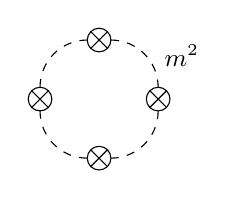
\begin{tikzpicture}[baseline={(0,0)}]
\begin{feynman}
\vertex (c) at (0,0);
\vertex [crossed dot] (x1) at (0,0.75) {};
\vertex [crossed dot] (x2) at (0.75,0) {};
\vertex [crossed dot] (x3) at (0,-0.75) {};
\vertex [crossed dot] (x4) at (-0.75,0) {};
\diagram*{
 (x1) -- [scalar, quarter left] (x2) -- [scalar, quarter left] (x3) -- [scalar, quarter left] (x4) -- [scalar, quarter left] (x1),
};
\end{feynman}
\node at (1.05,0.55) {\small $m^2$};
\end{tikzpicture}
&
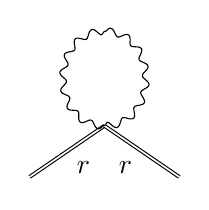
\begin{tikzpicture}[baseline={(0,0)}]
\begin{feynman}
\vertex (v) at (0,0);
\vertex (e1) at (-0.95,-0.65);
\vertex (e2) at (0.95,-0.65);
\vertex (t) at (0,1.2);
\diagram*{
 (e1) -- [double, edge label'=\(r\)] (v) -- [double, edge label'=\(r\)] (e2),
 (v) -- [boson, half left] (t) -- [boson, half left] (v),
};
\end{feynman}
\end{tikzpicture}
&
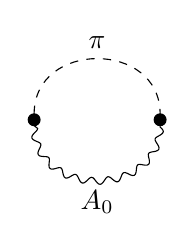
\begin{tikzpicture}[baseline={(0,0)}]
\begin{feynman}
\vertex (c) at (0,0);
\vertex [dot] (a) at (-0.8,0) {};
\vertex [dot] (b) at (0.8,0) {};
\diagram*{
 (a) -- [scalar, half left, edge label=\(\pi\)] (b) -- [photon, half left, edge label=\(A_0\)] (a),
};
\end{feynman}
\end{tikzpicture}
&
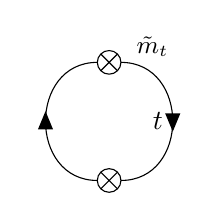
\begin{tikzpicture}[baseline={(0,0)}]
\begin{feynman}
\vertex (c) at (0,0);
\vertex [crossed dot] (a) at (0,0.75) {};
\vertex [crossed dot] (b) at (0,-0.75) {};
\diagram*{
 (a) -- [fermion, half left, edge label'=\(t\)] (b) -- [fermion, half left] (a),
};
\end{feynman}
\node at (0.55,0.95) {\small $\tilde m_t$};
\end{tikzpicture}
\\[2pt]
(a) & (b) & (c) & (d)\\[8pt]
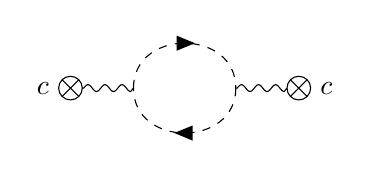
\begin{tikzpicture}[baseline={(0,0)}]
\begin{feynman}
\vertex (c) at (0,0);
\vertex (a) at (-0.65,0);
\vertex (b) at (0.65,0);
\vertex [crossed dot, label=left:\(c\)] (ca) at (-1.45,0) {};
\vertex [crossed dot, label=right:\(c\)] (cb) at (1.45,0) {};
\diagram*{
 (ca) -- [photon] (a) -- [charged scalar, half left] (b) -- [charged scalar, half left] (a),
 (b) -- [photon] (cb),
};
\end{feynman}
\end{tikzpicture}
&
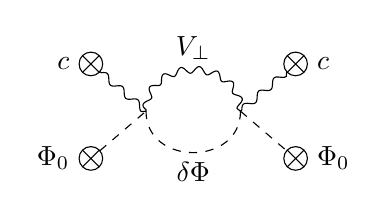
\begin{tikzpicture}[baseline={(0,0)}]
\begin{feynman}
\vertex (c) at (0,0);
\vertex (a) at (-0.6,0);
\vertex (b) at (0.6,0);
\vertex [crossed dot, label=left:\(c\)] (ca) at (-1.3,0.6) {};
\vertex [crossed dot, label=left:\(\Phi_0\)] (pa) at (-1.3,-0.6) {};
\vertex [crossed dot, label=right:\(c\)] (cb) at (1.3,0.6) {};
\vertex [crossed dot, label=right:\(\Phi_0\)] (pb) at (1.3,-0.6) {};
\diagram*{
 (ca) -- [photon] (a), (pa) -- [scalar] (a),
 (a) -- [photon, half left, edge label=\(V_\perp\)] (b) -- [scalar, half left, edge label=\(\delta\Phi\)] (a),
 (b) -- [photon] (cb), (b) -- [scalar] (pb),
};
\end{feynman}
\end{tikzpicture}
&
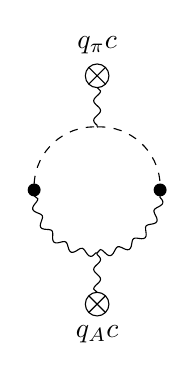
\begin{tikzpicture}[baseline={(0,0)}]
\begin{feynman}
\vertex (c) at (0,0);
\vertex [dot] (a) at (-0.8,0) {};
\vertex [dot] (b) at (0.8,0) {};
\vertex (m1) at (0,0.8);
\vertex (m2) at (0,-0.8);
\vertex [crossed dot, label=above:\(q_\pi c\)] (c1) at (0,1.45) {};
\vertex [crossed dot, label=below:\(q_A c\)] (c2) at (0,-1.45) {};
\diagram*{
 (a) -- [scalar, quarter left] (m1) -- [scalar, quarter left] (b) -- [photon, quarter left] (m2) -- [photon, quarter left] (a),
 (m1) -- [photon] (c1), (m2) -- [photon] (c2),
};
\end{feynman}
\end{tikzpicture}
&
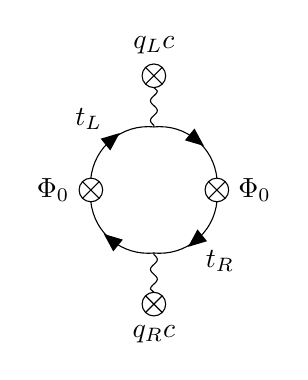
\begin{tikzpicture}[baseline={(0,0)}]
\begin{feynman}
\vertex (c) at (0,0);
\vertex [crossed dot, label=left:\(\Phi_0\)] (a) at (-0.8,0) {};
\vertex [crossed dot, label=right:\(\Phi_0\)] (b) at (0.8,0) {};
\vertex (m1) at (0,0.8);
\vertex (m2) at (0,-0.8);
\vertex [crossed dot, label=above:\(q_Lc\)] (c1) at (0,1.45) {};
\vertex [crossed dot, label=below:\(q_Rc\)] (c2) at (0,-1.45) {};
\diagram*{
 (a) -- [fermion, quarter left, edge label=\(t_L\)] (m1) -- [fermion, quarter left] (b) -- [fermion, quarter left, edge label=\(t_R\)] (m2) -- [fermion, quarter left] (a),
 (m1) -- [photon] (c1), (m2) -- [photon] (c2),
};
\end{feynman}
\end{tikzpicture}
\\[2pt]
(e) & (f) & (g) & (h)
\end{tabular}
\caption{One-loop diagrams of the finite-volume matching (non-zero modes in the loops; crossed dots are zero-mode backgrounds).
(a)~One tower of non-zero modes with any number of insertions of its field-dependent squared mass $m^2(r)$: the $\MSbar$ finite-volume energy $E_{\rm std}=D_\theta+V_{\rm CW}$ of Eq.~(\ref{eq:rb-Estd-def}).
(b)~Its first-order part, the tadpole $(T_\theta/2)\,m^2$ of Eq.~(\ref{eq:rb-tadpole}), shown for a gauge non-zero mode attached to the Higgs zero mode $r$ (double lines).
(c)~Longitudinal sector of a massive vector in Coulomb gauge: the Goldstone mode $\pi$ and the instantaneous Coulomb field $A_0$ mixed by $m_VA_0\dot\pi$ (dots), Eqs.~(\ref{eq:rb-coulomb-L})--(\ref{eq:rb-coulomb}).
(d)~Top-quark tower with insertions of $\tilde m_t=y_tr/\sqrt2$.
(e)--(h)~Terms of order $r^2c^2$ in a holonomy background $c$ (Sec.~\ref{sec:rb-r2c2}): (e)~twisted curvature of a charged tower (charged-component approximation); (f)~transverse vev mixing through the vertex $2(c\Phi_0)^\dagger V\delta\Phi$ of background-covariant Coulomb gauge; (g)~Coulomb mismatch, in which the Goldstone mode and the Gauss kernel are twisted by different charges $q_\pi\neq q_A$; (h)~top chiral loop, in which $t_L$ and $t_R$ are twisted by different charges and joined by the vev.}
\label{fig:rb-diagrams}
\end{figure}

\subsection{Renormalization-group consistency and the Coulomb-gauge anomalous dimension}
\label{sec:rb-rg}

The explicit $\mu$ dependence of $\Delta V_{\rm MC}$ must cancel the one-loop running of the couplings in the tree potential, up to a rescaling of the field.
We now show that this happens if and only if the Higgs field carries the Coulomb-gauge anomalous dimension.
Per real degree of freedom, Eq.~(\ref{eq:rb-VCW}) gives $\mu\partial_\mu V_{\rm CW}=-m^4/(32\pi^2)$, and the finite-volume parts $D_\theta$ do not depend on $\mu$.
Per massive vector the logarithmic coefficient of $\Delta V_{\rm MC}$ is $2a^2$ from the transverse modes and, by Eq.~(\ref{eq:rb-Delta-mu}), $a^2+b^2-2ab=(a-b)^2$ from the Coulomb mode, a total of $3a^2+b^2-2ab$.
Adding the radial mode and the top quark ($-12$ real degrees of freedom of mass $\tilde m_t$),
\begin{equation}
\mu\partial_\mu\Delta V_{\rm MC}=-\frac{1}{32\pi^2}\Bigl[6a_W^2+3a_Z^2+3b^2-2b(2a_W+a_Z)+(3\lambda r^2)^2-12\tilde m_t^4\Bigr].
\label{eq:rb-mudV}
\end{equation}
Inserting Eq.~(\ref{eq:rb-masses}),
\begin{equation}
\mu\partial_\mu\Delta V_{\rm MC}=-\frac{r^4}{32\pi^2}\Bigl[\tfrac{3}{16}\bigl(2g_2^4+g_Z^4\bigr)+12\lambda^2-3y_t^4-\tfrac{\lambda}{2}\bigl(3g_2^2+g_Y^2\bigr)\Bigr].
\label{eq:rb-mudV2}
\end{equation}
The one-loop running of the tree potential $\frac\lambda4r^4$ at fixed bare field is $\frac14\beta_\lambda^{(1)}r^4$, with
\begin{equation}
16\pi^2\beta_\lambda^{(1)}=24\lambda^2-6y_t^4+\tfrac38\bigl[2g_2^4+(g_2^2+g_Y^2)^2\bigr]+\lambda\bigl(12y_t^2-9g_2^2-3g_Y^2\bigr).
\label{eq:rb-betalam}
\end{equation}
The terms $g^4$, $\lambda^2$, and $y_t^4$ of Eq.~(\ref{eq:rb-mudV2}) cancel those of $\beta_\lambda^{(1)}$ one by one, and the sum leaves
\begin{equation}
\mu\partial_\mu\Delta V_{\rm MC}+\frac{\beta_\lambda^{(1)}}{4}r^4=\frac{\lambda r^4}{64\pi^2}\bigl(12y_t^2-6g_2^2-2g_Y^2\bigr)\equiv\gamma_\phi\,\lambda r^4 .
\label{eq:rb-rg}
\end{equation}
The remainder is the field rescaling $r\to r(1-\gamma_\phi\ln\mu)$ of the tree term, so the one-loop energy is scale independent if and only if
\begin{equation}
\gamma_\phi^{C}=\frac{3y_t^2-\frac32g_2^2-\frac12g_Y^2}{16\pi^2}.
\label{eq:rb-gammaC}
\end{equation}
This is the one-loop $R_\xi$ value at gauge parameter $\xi=1$; in $R_\xi$ gauges the gauge part is proportional to $3-\xi$.
The Landau-gauge counting, with $3a^2+b^2$ per vector and no term $-2ab$, requires the Landau value $(3y_t^2-\frac94g_2^2-\frac34g_Y^2)/(16\pi^2)$; the Coulomb counting has the additional term $-2b\sum_Va_V=-\lambda r^4(3g_2^2+g_Y^2)/2$, which raises $\gamma_\phi$ by $(3g_2^2+g_Y^2)/(64\pi^2)$ to Eq.~(\ref{eq:rb-gammaC}).
Numerically the left side of Eq.~(\ref{eq:rb-rg}) minus $\gamma_\phi^C\lambda r^4$ vanishes to $10^{-14}$ for $r=1$--$5$ at $\lambda=-0.010$. %
The unitary counting with $V_{\rm CW}$ leaves $3.8\times10^{-4}\times\lambda r^4/4$, the missing $b^2$ of the three Goldstone modes. %
With the couplings at $\mub$ of Sec.~\ref{rep:h-smmap} the Coulomb value is $\gamma_\phi^C=+2.1\times10^{-4}$ and the Landau value $-1.42\times10^{-3}$: the gauge and top parts nearly cancel in Coulomb gauge. %

The one-loop result is thus scale independent to this order, and the choice of $\mu$ is a convention.
We evaluate the matching and all couplings at $\mu=1/L$ and take the residual scale dependence as the two-loop error (Sec.~\ref{sec:rb-scale}).
The field normalization $\exp(-\gamma_\phi^C\ln c)$ that accompanies a scale change $\mu\to c\mu$ moves $m_c$ by at most $0.002\GeV$ even at $c=4\pi$. %

\paragraph{The top threshold.}
If the explicit top logarithm is moved together with $y_t$, the one-loop cancellation fails and $m_c$ moves by $\pm0.15\GeV$; this is the uncompensated $-6y_t^4/(16\pi^2)$ of $\beta_\lambda$, not a physical uncertainty. %
The consistent variation moves only the Yukawa coupling of the top loop, $y_t\to y_t(c_t\mu)$, and keeps its logarithm at $\mu$.
It probes the scale ambiguity of the finite-volume top term, $-12D_A(\tilde m_t^2)\simeq-12\cdot\frac{T_F}{2}\tilde m_t^2=+0.035\,r^2\propto y_t^2(\mu)$, which the two-loop QCD corrections to that term would compensate. %
The positive sign of this term means that the antiperiodic top tower stabilizes the zero mode, opposite to the periodic bosons.

\subsection{The slow coordinate and other one-loop countings}
\label{sec:rb-slow}

The slow coordinate is the radius $r$ of the Coulomb-gauge zero mode of the Higgs field, which has a flat measure and an exactly canonical kinetic term; this is the standard split of slow constant modes from fast non-zero modes on the torus~\cite{Luscher:1982ma,Koller:1987fq,vanBaal:2000zc}.
In this split the fast modes have $\omega\ge2\pi$, while the slow motion has a gap of about $1.5$. %

A natural alternative is the gauge-invariant zero mode $\rho_0$ of $|\Phi(\bm x)|$, for which the Goldstone modes are absorbed and each vector has three polarizations of mass $a$ (unitary counting).
Expanding $|\Phi|=r+\delta\rho+\sum_a\pi_a^2/(2r)+\dots$ gives
\begin{equation}
\rho_0=|\Phi_0|+C(r),\qquad C(r)=\sum_a\frac{\langle\pi_a^2\rangle_{\rm FV}}{2r}.
\label{eq:rb-rho0}
\end{equation}
We find $rC=-0.33868$ as $r\to0$, equal to $3T_B/2$, and $-0.3432$, $-0.3568$, and $-0.3892$ at $r=1.5$, $3$, and $5$. %
To first order in $b$ the Coulomb energy and the unitary energy with $V_{\rm CW}$ differ by exactly $V'_{\rm tree}(r)\,C(r)$, which is the origin of their difference.

The unitary counting is not a controlled Born--Oppenheimer variable, for three reasons.
(i)~The metric of the fast angular modes is proportional to $\rho_0^2$, so at fixed canonical fast variables $\partial_{\rho_0}$ acquires a term $(\pi/\rho_0)\partial_\pi$; this generates diagonal Born--Oppenheimer terms and an induced mass of the same order as the Goldstone term.
(ii)~The polar measure $\prod_{\bm x}\rho(\bm x)^3$ has weight $1+Z(0)=0$ under $\zeta$ regularization, which removes the meaning of the centrifugal term $3/(8\rho^2)$, and $|\Phi|$ is a composite operator that needs its own renormalization.
(iii)~The unitary result cannot be repaired by shifting the coordinate: replacing $r$ by $r+C(r)$ in the full potential shifts the gauge zero-point energy and the centrifugal term by $0.06$--$0.15/L$, much more than the Goldstone term, and $r+C(r)$ vanishes at $r\approx0.58$. %
The shift of the gauge zero-point energy is the seagull part of the cross terms of Sec.~\ref{rep:h-cross}, not a kinetic factor.

Within the Coulomb split the residual Born--Oppenheimer corrections are small.
The diagonal term $E_{\rm BH}=\sum\frac1{16}[d\ln(Z\omega)/dr]^2\simeq1.1\times10^{-4}\,r^2$ corresponds to $\delta m^2\approx2\times10^{-4}$, about $1/30$ of the first-order Goldstone term $0.0034\,r^2$, and the induced mass $\delta M=5\times10^{-5}$--$5\times10^{-4}$ changes the tunneling exponent by less than $10^{-4}$. %
Together they move $m_c$ by at most $0.002\GeV$, the Born--Oppenheimer part of the matching error. %

Table~\ref{tab:rb-countings} compares the countings in the one-dimensional model of the matching study, with the earlier mapping. %
Only the Landau-gauge counting with $V_{\rm CW}$ comes close to the Coulomb result, as expected for $m_V\ll2\pi/L$; the remaining difference comes from the Coulomb weight $(1+a/k^2)^{1/2}$ and the terms of order $b^2$.
Shifting only the tree and matching parts of the unitary potential by $C(r)$ moves $m_c$ by $+0.011$ and $+0.015\GeV$ at $\Pone=0.9$ and $1/2$; the difference is $C\,dV'_{\rm match}$, formally of higher order in $\hbar$ but as large as the Goldstone term because $V'_{\rm tree}\sim\lambda r^3$ is small. %
A renormalization-group improvement with $\mu^2=(1+r^2)/L^2$ resums logarithms $\ln(m^2L^2)$ that do not exist in finite volume: for $r\le5$ every field-dependent mass is at least $3.6$ times below $2\pi/L$, and $m_Z$ reaches $2\pi/L$ only at $r\approx18$, so the resulting shift of about $+0.13\GeV$ is spurious. %

\begin{table}[t]
\centering
\caption{One-loop countings of the matching in the one-dimensional model of the matching study.
The width $\Gamma$ (units $1/L$) is evaluated at $\lambda=-0.010$ with the fixed couplings; the shift of the critical top mass (GeV) relative to the Coulomb counting uses the hazard with the earlier Standard Model mapping. %
The Coulomb result of this model is $m_c=172.35$ and $172.77\GeV$ at $\Pone=0.9$ and $1/2$.} %
\label{tab:rb-countings}
\begin{tabular}{lccc}
\toprule
Counting & $10^3\,\Gamma$ & $\Delta m_c(0.9)$ & $\Delta m_c(0.5)$ \\
\midrule
Unitary, $D_\theta$ only & $2.051$ & $-0.138$ & $-0.184$ \\ %
Unitary with $V_{\rm CW}$ & $1.510$ & $-0.072$ & $-0.112$ \\ %
Landau, $D_\theta$ only & $1.433$ & $-0.081$ & $-0.092$ \\ %
Landau with $V_{\rm CW}$ & --- & $-0.012$ & $-0.016$ \\ %
Coulomb (this work) & $0.987$ & $0$ & $0$ \\ %
\bottomrule
\end{tabular}
\end{table}

\subsection{One-loop terms of order \texorpdfstring{$r^2c^2$}{r2c2}: vev mixing, Coulomb mismatch, and the top chiral loop}
\label{sec:rb-r2c2}

The gauge zero modes are constant connections, and charged non-zero modes in their background have twisted boundary conditions.
Expanded to second order in the holonomy $c$, this gives the cross terms of Sec.~\ref{rep:h-cross}.
In the charged-component approximation (CCA) of that section each real degree of freedom contributes the curvature of the twisted image sum, Eq.~(\ref{eq:rb-Etheta}), with its own mass and charge [Fig.~\ref{fig:rb-diagrams}(e)].
Along the broken direction three further one-loop terms of order $r^2c^2$ enter, and here we derive them and show that together they make $\mu=1/L$ a consistent matching scale for the cross terms.

\paragraph{The CCA curvature has no logarithm.}
For a charged mode with $\omega=(|\bm k-q\bm c|^2+m^2)^{1/2}$ the second derivative at $\bm c=0$, averaged over directions, is $q^2\sum_{\bm k}'(1/\omega-k^2/3\omega^3)=q^2\sum_{\bm k}'(2k^2+3m^2)/(3\omega^3)$.
At large $k$,
\begin{equation}
\frac{2k^2+3m^2}{3\omega^3}=\frac{2}{3k}\Bigl(1+\frac{3m^2}{2k^2}\Bigr)\Bigl(1-\frac{3m^2}{2k^2}+O(k^{-4})\Bigr)=\frac{2}{3k}+O(k^{-5}),
\label{eq:rb-noLog}
\end{equation}
so the $m^2/k^3$ terms cancel and the curvature carries no $\ln\mu$.
Any scale dependence of the $r^2c^2$ sector must therefore come from the terms below.

\paragraph{Vev mixing in background-covariant Coulomb gauge.}
The twisted transverse modes of the CCA are exact eigenmodes only in background-covariant Coulomb gauge, $D^{\rm bg}\cdot V\equiv\nabla\cdot V-i[c,V]=0$, so the Higgs--gauge vertex must be taken in that gauge.
Write $D_i(\Phi_0+\delta\Phi)$ with $D_i=\partial_i-ic_i-iV_i$, where $c$ is the constant holonomy (couplings absorbed), $V$ the gauge non-zero mode, and $\delta\Phi$ the Higgs non-zero mode.
The terms of $|D_i\Phi|^2$ bilinear in $V$ and $\delta\Phi$ are
\begin{equation}
i\Phi_0^\dagger V_i\,D^{\rm bg}_i\delta\Phi+\Phi_0^\dagger c_iV_i\,\delta\Phi+{\rm h.c.},\qquad D^{\rm bg}_i=\partial_i-ic_i .
\label{eq:rb-vev-raw}
\end{equation}
Integrating the first term by parts and using the gauge condition $\partial_iV_i=i[c_i,V_i]$,
\begin{equation}
i\Phi_0^\dagger V_i\partial_i\delta\Phi\to-i\Phi_0^\dagger(\partial_iV_i)\delta\Phi=\Phi_0^\dagger[c_i,V_i]\delta\Phi,
\label{eq:rb-vev-parts}
\end{equation}
and adding the remaining pieces, $\Phi_0^\dagger\bigl([c,V]+Vc+cV\bigr)\delta\Phi=2\Phi_0^\dagger c\cdot V\delta\Phi$.
The vertex is therefore
\begin{equation}
\mathcal L_{\rm mix}=2\,(c\Phi_0)^\dagger V\cdot\delta\Phi+{\rm h.c.},
\label{eq:rb-vev-vertex}
\end{equation}
the analogue of $2p\cdot V$ in covariant diagrams, with $c$ in the role of the external momentum.
In ordinary Coulomb gauge, $\nabla\cdot V=0$, the same steps give the anticommutator $\Phi_0^\dagger\{c,V\}\delta\Phi$, which differs by a commutator and misses the non-abelian channels.
For a $W^1$ background the vertex (\ref{eq:rb-vev-vertex}) mixes the gauge and Higgs non-zero modes in the channels $W^1\to\delta\rho$, $B\to\pi^1$, $W^2\to\pi^3$, and $W^3\to\pi^\pm$; for a $Z$ background $W^{1,2}$ mix with $\pi^\pm$ with coupling $g_Zg_2$; for a photon background the vertex vanishes because $Q\Phi_0=0$.
The channel strengths are $3g_2^2+g_Y^2$ in the $W$ direction and $g_Z^2+2g_2^2$ in the $Z$ direction, both proportional to $(3g_2^2+g_Y^2)$ times the tree term.

At second order each channel lowers the energy [Fig.~\ref{fig:rb-diagrams}(f)],
\begin{equation}
\delta H\propto-r^2c_{\rm pol}\,S(m_1^2,m_2^2),\qquad S(m_1^2,m_2^2)=\sum_{\bm k}{}'\frac{1}{\omega_1\omega_2(\omega_1+\omega_2)},
\label{eq:rb-bubble}
\end{equation}
with $c_{\rm pol}=\frac23$ exactly, because only transverse fluctuations mix in Coulomb gauge and the transverse projector averages to $(d-1)/d$.
The bubble $S$ diverges logarithmically and is defined in $\MSbar$ through $S=-4\,d^2E_{\rm std}/d(m^2)^2$ plus an absolutely convergent difference; for equal masses $S=\sum'1/(2\omega^3)$ is exactly $-4\,d^2E_{\rm std}/d(m^2)^2$.
From Eq.~(\ref{eq:rb-Estd}),
\begin{equation}
S(0,0)=-8\Bigl[c_2-\frac{\ln\mu^2L^2+\frac32}{64\pi^2}\Bigr]=-0.0311\ \ (\mu=1/L),\qquad \frac{dS}{d\ln\mu}=\frac{1}{4\pi^2}, %
\label{eq:rb-S0}
\end{equation}
negative because the infrared cutoff $2\pi/L$ of the non-zero modes exceeds $\mu=1/L$; at $\mu=2\pi/L$ it is $+0.016$. %
Each term alone therefore changes sign between $\mu=1/L$ and $2\pi/L$, and only the sum of all $r^2c^2$ terms is meaningful.

\paragraph{Coulomb mismatch.}
The Goldstone mode and the Gauss kernel that eliminates $A_0$ are twisted by different charges, $\Delta q=q_\pi-q_A=g_Z/2$ in a $Z$ background and $\Delta q=0$ in a photon background, whereas the CCA gives the Coulomb mode the Goldstone twist with $\omega^2=k^2+a+b$ [Fig.~\ref{fig:rb-diagrams}(g)].
Repeating the derivation of Eq.~(\ref{eq:rb-coulomb}) with twisted momenta, the exact Coulomb frequency in the charged sector is
\begin{equation}
\omega_C^2=\frac{(|\bm k-q_\pi\bm c|^2+b)(|\bm k-q_A\bm c|^2+a)}{|\bm k-q_A\bm c|^2},
\label{eq:rb-omegaC-twist}
\end{equation}
and in the neutral sector we diagonalize the $(\delta\rho,\pi^3,Z_0)$ system with kinetic matrix ${\rm diag}(1,Z_k)$ and the twist coupling $2tk_x$ of $\delta\rho$ and $\pi^3$.
The difference from the CCA falls as $C_{\rm C}/(2k^3)$, a logarithm, with $C_{\rm C}=2a_W(g_Z/2)^2/3$ in the charged sector (fit over analytic $1.003$) and $C_{\rm C}=0.353\,a_Z(g_Z/2)^2$ in the neutral sector, $6\%$ off the expected $1/3$. %
The finite Coulomb part is $-0.27$ times the transverse vev mixing for $r\ge2$; in the $W$ direction, where we did not compute it directly, we use this ratio, as the custodial limit $g_Y\to0$ suggests, with a $25\%$ error. %

\paragraph{Top chiral loop.}
The two chiralities of the top quark carry different charges, so in a holonomy background along the broken direction $t_L$ and $t_R$ are twisted differently, while the vev joins them through $y_t$ [Fig.~\ref{fig:rb-diagrams}(h)].
Gauge invariance of the Yukawa term fixes the difference of the two twists to the charge $q_\Phi$ of the vev component.
We diagonalize the chiral Dirac Hamiltonian exactly on each antiperiodic mode, using a $6\times6$ matrix for $t_L\leftrightarrow b_L$ in the $T^1$ direction, take the second derivative in the background numerically, and subtract the CCA value.
The difference falls as $B/(2k^3)$, the axial logarithm, and in the $T^3$, $Y$, $T^3+Y$, and $T^1$ directions $B/(q_\Phi^2\tilde m_t^2)=1.000\pm0.001$ per color. %
The finite part, $\approx q_\Phi^2\tilde m_t^2S_A(\tilde m_t^2)$ with $S_A=-0.021$ to $-0.028$, is negative and softens the gauge zero modes. %

\paragraph{Renormalization-group closure.}
In units of $c$ the tree-level Higgs--gauge-zero-mode term $\Phi^\dagger(c\cdot T)^2\Phi$ contains no coupling, because $g\,c$ is not renormalized in background-field gauge.
Its only scale dependence comes from the Higgs field normalization, $d\ln({\rm tree})/d\ln\mu=-2\gamma_\phi^C$, so the logarithms of all one-loop $r^2c^2$ terms must add up to $+2\gamma_\phi^C$ times the tree term.
The CCA curvature has none [Eq.~(\ref{eq:rb-noLog})].
The top chiral loop gives exactly the top part, $3y_t^2$ in the numerator of Eq.~(\ref{eq:rb-gammaC}).
The transverse vev mixing gives exactly $4/3$ of the gauge part in both the $W$ and $Z$ directions: in units in which the gauge part of $\gamma_\phi$ is $3-\xi$, so that Eq.~(\ref{eq:rb-gammaC}) carries $2$, the transverse Coulomb-gauge bubbles carry $\frac83$.
The Coulomb mismatch supplies $-\frac13$, the remaining $-\frac23$ units.
In the $Z$ direction the computed sum, $\frac43-0.34$, closes on the requirement to $0.994$, $0.973$, $0.993$, and $0.990$ at $r=2$, $3$, $4$, and $5$. %
At $r=1$ the fit of the $k^{-3}$ coefficient is noisy (closure $0.87$), so the main calculation scales $C_{\rm C}\propto r^2$ from $r=5$. %
Hence $\mu=1/L$ is a consistent matching scale for the cross terms as well: moving the one-loop terms and the Higgs normalization together from $1/L$ to $2\pi/L$ changes the result only through two-loop terms and the closure residual of at most $3\%$. %

In the final model these terms shift the critical mass, relative to the CCA, by $+0.021$, $+0.028$, and $+0.034\GeV$ (gauge part) and $-0.017$, $-0.022$, and $-0.027\GeV$ (top chiral loop) at $\Pone=0.9$, $0.5$, and $0.1$, a net $+0.005$, $+0.006$, and $+0.007\GeV$. %
The cancellation is the one required by the small value $\gamma_\phi^C\approx2\times10^{-4}$ of Eq.~(\ref{eq:rb-gammaC}). %

\subsection{Matching-scale dependence in the final model}
\label{sec:rb-scale}

The two-loop finite-volume matching is not computed; we estimate it by the dependence on the matching scale.
We set $\mu=c\,\mub/(\cosh2\tau)^{1/2}$ at every node of the hazard of Sec.~\ref{rep:h-survival} and repeat the full node-by-node calculation of the final model in four steps.
(i)~The tree-level quartic, the matching $\Delta V_{\rm MC}$, the gauge profiles, the cross terms, and $g_3$ take their couplings at $c\mu$, and the conditional Gaussian of the gauge zero modes is recomputed with $g(c\mu)$.
(ii)~The matching is $\MSbar$-subtracted at $(\mu L)^2=c^2$, and the field normalization $\exp(-\gamma_\phi^C\ln c)$ multiplies $\frac\lambda4r^4$ and $\Delta V_{\rm MC}$, which keeps the $r$ sector one-loop consistent (Sec.~\ref{sec:rb-rg}).
(iii)~In the $r^2c^2$ sector neither the tree-level normalization nor the explicit subtraction scale of the cross terms moves.
This is equivalent to moving both, because the one-loop logarithms of that sector close on $2\gamma_\phi^C$ times the tree term to $97$--$99\%$; the error of this step is at most $3\%$ of $2\gamma_\phi^C\ln c$ times the tree term and negligible. %
(iv)~The top threshold $c_t$ moves the Yukawa coupling of every top loop, in $\Delta V_{\rm MC}$ and in the cross terms, to $c_t\mu$ and keeps the explicit logarithms at $\mu$.
Each variant uses the final roots as seeds and the same windows, for ten top masses and eleven nodes.
For $c=1$ the recomputed roots reproduce the final ones to $2\times10^{-12}$, and so do the critical masses (in GeV); none of the 66 node jobs of the six variants needed rescue. %

\begin{table}[t]
\centering
\caption{Shift of the critical top mass (GeV) under a change of the matching scale $\mu\to c\,\mu$ or of the top-threshold scale $\mu\to c_t\,\mu$ in the final model, relative to $c=c_t=1$, at $\alpha_s(M_Z)=0.1180$, and the adopted matching item of the error budget.} %
\label{tab:rb-muscan}
\begin{tabular}{lccc}
\toprule
Variant & $\Pone=0.9$ & $\Pone=0.5$ & $\Pone=0.1$ \\
\midrule
$c=\frac12$ & $+0.0022$ & $+0.0054$ & $+0.0080$ \\ %
$c=2$ & $-0.0095$ & $-0.0128$ & $-0.0160$ \\ %
$c=2\pi$ & $-0.0391$ & $-0.0489$ & $-0.0582$ \\ %
$c_t=\frac12$ & $+0.0084$ & $+0.0120$ & $+0.0153$ \\ %
$c_t=2$ & $-0.0082$ & $-0.0117$ & $-0.0150$ \\ %
\midrule
Adopted & $^{+0.009}_{-0.039}$ & $^{+0.012}_{-0.049}$ & $^{+0.015}_{-0.058}$ \\ %
\bottomrule
\end{tabular}
\end{table}

Table~\ref{tab:rb-muscan} lists the shifts.
Within $c\in[\frac12,2]$ the change is carried almost entirely by the top Yukawa coupling of the finite-volume top term: $c=2$ and $c_t=2$ give nearly the same shift.
At $c=2\pi$ a curvature of order $\ln^2c$ appears, the signature of the two-loop terms.
The shifts are of the same size as in the one-dimensional matching study with the earlier mapping ($c=2\pi$: $-0.034$ and $-0.043\GeV$; $c_t\in[\frac12,2]$: $\pm0.009$ and $\pm0.012\GeV$ at $\Pone=0.9$ and $1/2$) and about $15\%$ larger at $c=2\pi$. %
The closure of the cross-term logarithms does not reduce this item, because the scan probes the $r$ sector, where the two-loop finite-volume top term dominates.

The scale and threshold variations probe the same source, $y_t(\mu)$ in the finite-volume top term, so we take their envelope on each side rather than their quadrature sum.
To it we add in quadrature the Born--Oppenheimer item, $0.002\GeV$, of Sec.~\ref{sec:rb-slow}, and we use the conservative range $c\in[\frac12,2\pi]$, which extends beyond the natural scale $\mu_*=3.41/L$ of Eq.~(\ref{eq:rb-mustar}); this one-sided extension is why the item is asymmetric. %
The result is the matching row of the error budget, $^{+0.009}_{-0.039}$, $^{+0.012}_{-0.049}$, and $^{+0.015}_{-0.058}\GeV$ at $\Pone=0.9$, $0.5$, and $0.1$; a quadrature sum would add at most $0.002\GeV$ on either side. %
The entries at $\Pone=0.1$ are computed directly.
The estimate assumes that the two-loop finite-volume terms have no unusually large constant.

\section{Higgs zero mode II: reduced model, resonance and width}\label{rep:h-reduced}

We solve the zero-mode problem of Sec.~\ref{rep:h-matching} in a model with two coordinates, the Higgs radius $r$ and the modulus $s=|\bm w|$ of the hypercharge zero mode, with the SU(2) zero modes in a conditional Gaussian.
We show that the Gaussian factorizes exactly, that the hypercharge zero mode is not fast where the Higgs zero mode sits and must be treated jointly with $r$, and that the resulting two-dimensional model reproduces the full sixteen-dimensional ground state at $\lambda=0$ to $0.003/L$. %
For $\lambda<0$ the electroweak state is a finite-volume resonance with complex energy $E=\varepsilon-i\Gamma/2$; we compute $\Gamma$ as a multichannel Siegert state and confirm it with absorbing potentials and real-wall stabilization.
Full-dimensional diffusion Monte Carlo (DMC) with a gauge-invariant wall confirms the resonance energy to $0.005/L$, and four independent estimates give the same width to within $8\%$.
Together they would raise the critical top mass by $+0.005\GeV$ at $\Pone=0.9$ and $+0.008\GeV$ at $\Pone=1/2$ (Sec.~\ref{rep:v-fulldim}); the central values do not include this shift, which lies inside the one-sided full-dimensional item of the error budget. %
Finally we explain the size of the threshold: near threshold $\ln\Gamma=a-b|\lambda|^{-1/2}$, and the closed form $|\lamc|^{1/2}\simeq b_{\rm eff}/\ln(A_{\rm eff}\eta_\infty/\ln2)$, with the effective slope $\sigma_{\rm eff}=0.44$ and the prefactor $A_{\rm eff}\simeq310$ fixed by the computed threshold, shows that the confinement slope sets the size of $\lamc$ and that the duration of the turn enters only logarithmically. %
Under assumption (A5) of Sec.~\ref{rep:setup} the zero-mode dynamics is that of this model, with the residual errors collected in Sec.~\ref{rep:h-budget}.

\subsection{Conditional Gaussian of the gauge zero modes and its exact factorization}
\label{sec:rb-gauss}

At fixed $r$ we take the state of the gauge zero modes from the most general central Gaussian that is invariant under spatial rotations and residual U(1)$_{\rm em}$.
Different spatial directions are uncorrelated, because a two-point function of spatial vectors can only be proportional to $\delta_{ij}$.
In each direction the precision matrix on $y_i=(x_i^1,x_i^2,x_i^3,w_i)$ is ${\rm diag}(a,a,K_2)$, where U(1)$_{\rm em}$ invariance forces the two charged components $x^{1,2}$ to share one parameter $a$ and decouple, and
\begin{equation}
K_2=\begin{pmatrix}k&c\\ c&e\end{pmatrix},\qquad D=ke-c^2 .
\label{eq:rb-K2}
\end{equation}
(The parameter $c$ of $K_2$ is a Gaussian parameter, not the holonomy of Sec.~\ref{sec:rb-r2c2}.)
Completing the square in the neutral block,
\begin{equation}
k\,(x^3)^2+2c\,x^3w+e\,w^2=k\,(x^3+\beta w)^2+\tilde e\,w^2,\qquad \beta=\frac ck,\qquad \tilde e=e-\frac{c^2}{k},
\label{eq:rb-square}
\end{equation}
so the Gaussian factorizes exactly into a conditional state of the SU(2) modes and a marginal state of the hypercharge mode,
\begin{align}
\Psi&=\varphi(\bm x|\bm w)\,\chi(\bm w),\qquad \chi\propto e^{-\tilde e\,|\bm w|^2/2},\nonumber\\
\varphi&\propto \prod_i \exp\Bigl\{-\tfrac12\Bigl[a\bigl((x_i^1)^2+(x_i^2)^2\bigr)+k\bigl(x_i^3+\beta w_i\bigr)^2\Bigr]\Bigr\}.
\label{eq:rb-condGauss}
\end{align}
For $\psi\propto\exp(-\frac12y^{\mathsf T}Ky)$ one has $\langle p_ip_j\rangle=K_{ij}/2$ and $\langle y_iy_j\rangle=(K^{-1})_{ij}/2$, and all moments of Eq.~(\ref{eq:rb-H0}) are elementary~\cite{Luscher:1982ma,vanBaal:2000zc}:
\begin{align}
\bigl\langle\tfrac12p^2\bigr\rangle&=\tfrac34(2a+k+e),\nonumber\\
\bigl\langle\tfrac12y^{\mathsf T}\mathcal My\bigr\rangle&=\frac{3r^2}{16}\Bigl[\frac{2g_2^2}{a}+\frac{g_2^2e-2g_2g_Yc+g_Y^2k}{D}\Bigr],\nonumber\\
\Bigl\langle\frac{g_2^2}{4}\sum_{ij}|\bm x_i\times\bm x_j|^2\Bigr\rangle&=\frac{3g_2^2}{4a^2}+\frac{3g_2^2e}{2aD},\nonumber\\
\frac{2}{r^2}\bigl\langle(L^1)^2+(L^2)^2\bigr\rangle&=\frac{3}{ar^2}\,\frac{e(k-a)^2-2c^2(k-a)+kc^2}{D},
\label{eq:rb-moments}
\end{align}
where $\mathcal M$ is the mass matrix of Eq.~(\ref{eq:rb-massmatrix}) and the last line follows from $L^1\chi=i\,x^2[(k-a)x^3+cw]\chi$, the action of an SU(2) rotation about the 1-axis on the Gaussian.
In terms of $\beta$ and $\tilde e$ the sum of the four moments takes the form
\begin{align}
E_{\rm tot}&=C_0+\frac34\Bigl(\tilde e+\frac{\Omega^2}{\tilde e}\Bigr),\nonumber\\
\Omega^2&=\frac{r^2}{4}(g_Y-g_2\beta)^2+\frac{2g_2^2\beta^2}{a}+\frac{4a\beta^2}{r^2},
\label{eq:rb-Etot}
\end{align}
with
\begin{equation}
C_0=\tfrac34(2a+k)+\tfrac34k\beta^2+\frac{3r^2}{16}\Bigl(\frac{2g_2^2}{a}+\frac{g_2^2}{k}\Bigr)+\frac{3g_2^2}{4a^2}+\frac{3g_2^2}{2ak}+\frac{3(k-a)^2}{akr^2}.
\label{eq:rb-C0}
\end{equation}
The three terms of $\Omega^2$ come from the Higgs mass term, in which $x^3=-\beta w+\delta x^3$ leaves $(g_Y-g_2\beta)w$ in the massive combination, from the magnetic quartic, and from the angular term of Eq.~(\ref{eq:rb-bodyframe}).
The hypercharge mode is a harmonic oscillator of frequency $\Omega$, so the minimization over $\tilde e$ gives $\tilde e=\Omega$ and $E_{\rm tot}=C_0+\frac32\Omega$.
We minimize over the remaining parameters $(a,k,\beta)$ globally from many starting points and by Newton continuation in $r$; at six radii the global minima agree with the continuation to $4\times10^{-15}$. %

\paragraph{Born--Huang term.}
When the gauge state follows $r$ adiabatically, the radial motion acquires the Born--Huang term $B_r=\frac12\langle\partial_r\Psi|\partial_r\Psi\rangle=\frac{3}{16}{\rm tr}[(K^{-1}K')^2]$, with $K'$ obtained by implicit differentiation of the stationarity conditions rather than by differences.
It splits exactly into
\begin{align}
B_x&=\frac{3}{16}\Bigl[2\Bigl(\frac{a'}{a}\Bigr)^2+\Bigl(\frac{k'}{k}\Bigr)^2\Bigr],\qquad
B_w=\frac{3}{16}\Bigl(\frac{\tilde e'}{\tilde e}\Bigr)^2,\nonumber\\
B_\beta&=\frac{3k\beta'^2}{8\tilde e}=\Bigl\langle\frac k4\beta'^2|\bm w|^2\Bigr\rangle_\chi .
\label{eq:rb-BH}
\end{align}
At small $r$ the mass term dominates $\Omega$, $\tilde e=\Omega\simeq g_Yr/2$, and therefore
\begin{equation}
B_w=\frac{3}{16}\Bigl(\frac{\Omega'}{\Omega}\Bigr)^2\xrightarrow{\;r\to0\;}\frac{3}{16r^2};
\label{eq:rb-Bw}
\end{equation}
numerically $r^2B_w=0.1875000$ at $r=0.004$. %
The moments, the factorization, and Eqs.~(\ref{eq:rb-C0})--(\ref{eq:rb-BH}) were rederived symbolically with Gaussian expectation values in Wolfram Language; the six identities vanish identically and hold numerically to $10^{-14}$ at all $r$. %

\paragraph{The hypercharge zero mode is not fast.}
A term $3/(16r^2)$ is as singular as the centrifugal term $3/(8r^2)$ and would raise the Frobenius exponent of the radial function from $3/2$ to $1.6726$ [from $s_0(s_0-1)/2=\frac38+\frac3{16}$]. %
Its origin is unphysical: the hypercharge oscillator has frequency $\Omega\propto r$, so it is soft exactly where the Higgs zero mode sits, and the adiabatic assumption fails there.
Table~\ref{tab:rb-BH} shows the consequences in the $\lambda=0$ ground state of the two-dimensional model below.
$B_w$ is $0.44$ at $r=0.65$ and $0.18$ at $r=1$; the exact conditional width $\langle s^2\rangle$ saturates near $5$, whereas the adiabatic value $3/(2\Omega)$ grows to $11$--$17$ at $r=0.4$--$0.6$, which softens the inner wall. %
In the barrier region, $r\approx3$--$5.5$, $B_w<0.006$ is smaller than $B_x$ and $B_\beta$, and $\bm w$ follows its local ground channel. %
Beyond $r\approx2$ the soft direction turns from $\bm w$ into the photon combination: $\beta$ grows from $0.1$ to $0.76$. %
A one-dimensional Born--Oppenheimer reduction in $r$ is therefore unreliable in the well and adequate under the barrier.

\begin{table}[t]
\centering
\caption{Born--Huang terms and conditional width of the hypercharge mode in the $\lambda=0$ ground state of the two-dimensional model, compared with the Born--Oppenheimer width $3/(2\Omega)$; the last column is the radial probability density.} %
\label{tab:rb-BH}
\begin{tabular}{ccccccc}
\toprule
$r$ & $\Omega$ & $B_x$ & $B_w$ & $\langle s^2\rangle$ & $3/(2\Omega)$ & $\rho(r)$ \\
\midrule
$1.0$ & $0.219$ & $0.0024$ & $0.176$ & $4.90$ & $6.79$ & $0.51$ \\ %
$1.5$ & $0.320$ & $0.0048$ & $0.066$ & $4.55$ & $4.65$ & $0.68$ \\ %
$2.0$ & $0.407$ & $0.0075$ & $0.028$ & $4.15$ & $3.60$ & $0.46$ \\ %
$3.0$ & $0.530$ & $0.0115$ & $0.0053$ & $3.49$ & $2.79$ & $0.05$ \\ %
\bottomrule
\end{tabular}
\end{table}

\subsection{The two-dimensional Hamiltonian}
\label{sec:rb-2d}

We keep $\varphi(\bm x|\bm w)$ at the pointwise optimal parameters and replace $\chi(\bm w)$ by a function $\chi(r,\bm w)$ that we solve for.
Because $\varphi$ is real and normalized, $\langle\varphi|\partial\varphi\rangle=0$, the cross terms of the kinetic energy vanish, and the projection onto the trial family $\chi(r,\bm w)\varphi(\bm x|r,\bm w)$ is exact: $\frac12\langle|\partial_{\bm w}\varphi|^2\rangle=\frac34k\beta^2$ is part of $C_0$, and $\frac12\langle|\partial_r\varphi|^2\rangle=B_x+\frac k4\beta'^2|\bm w|^2$ adds to the stiffness of $\bm w$.
Acting on $u=r^{3/2}f$, the model Hamiltonian is
\begin{align}
H_{\rm 2D}={}&-\tfrac12\partial_r^2+\frac{3}{8r^2}-\tfrac12\Delta_w+C_0+B_x+\tfrac12\Omega_{\rm eff}^2|\bm w|^2\nonumber\\
&+\frac{\lambda}{4}r^4+\Delta V_{\rm MC}(r)+\delta E_{\rm DMC}(r),\qquad \Omega_{\rm eff}^2=\Omega^2+\frac k2\beta'^2 ,
\label{eq:rb-H2D}
\end{align}
with $\Delta V_{\rm MC}$ of Eq.~(\ref{eq:rb-dVMC}).
We keep the s wave of $\bm w$, with $v=s\chi$ and $v(0)=0$, and write the $r$-dependent part as
\begin{equation}
U_1(r)=\frac{3}{8r^2}+C_0+B_x+\frac\lambda4r^4+\Delta V_{\rm MC}+\delta E_{\rm DMC},\qquad
H_{\rm 2D}=-\tfrac12\partial_r^2+U_1(r)-\tfrac12\Delta_w+\tfrac12\Omega_{\rm eff}^2|\bm w|^2 . %
\label{eq:rb-U1}
\end{equation}
The cross terms of Sec.~\ref{rep:h-cross} add further terms to $U_1$ and to the $\bm w$ channel.

The term $\delta E_{\rm DMC}(r)=E_{\rm tot}^{\rm ex}(r)-E_{\rm tot}(r)$ corrects the Gaussian shape of the SU(2) modes.
Here $E_{\rm tot}^{\rm ex}(r)$ is the lowest eigenvalue of the gauge Hamiltonian plus the angular term $(2/r^2)[(L^1)^2+(L^2)^2]$ at fixed $r$, computed by rotating-frame DMC in the body frame, so that $E_{\rm g}^{\rm ex}\le E_{\rm tot}^{\rm ex}\le E_{\rm tot}$.
We interpolate it with a cubic spline of zero slope at $r=0$ and freeze it beyond $r=9$.
With $\delta E_{\rm DMC}$ the fixed-$r$ energy of the model equals the exact $E_{\rm tot}^{\rm ex}$.
It is the one ingredient that keeps the fixed couplings; the node couplings differ from them by at most $0.6\%$ for $\tau\le1$, where the hazard has most of its weight, which moves $m_c$ by an estimated $0.002\GeV$ or less. %
Without $\delta E_{\rm DMC}$ the model (denoted 2D$_{\rm G}$) solves exactly for the trial family and is therefore a strict variational upper bound on the full-dimensional energy at $\lambda=0$.
Removing the $\bm w$ dynamics again gives two Born--Oppenheimer models that bracket the two-dimensional result: keeping $B_w$ gives an upper bound, and dropping it gives the adiabatic lower bound.

\begin{table}[t]
\centering
\caption{Ground-state energy at $\lambda=0$ (units $1/L$; local model without the matching term) for the reductions of the text, compared with full-dimensional DMC, $4.4478(13)$~\cite{Kosztin:1996fh,Foulkes:2001zz}.} %
\label{tab:rb-lam0}
\begin{tabular}{lcc}
\toprule
Reduction & $L\varepsilon_0$ & Difference \\
\midrule
One-dimensional, Gaussian (with $B_r$) & $4.5985$ & $+0.151$ \\ %
One-dimensional, exact gauge shape & $4.5434$ & $+0.096$ \\ %
Born--Oppenheimer bound, with $B_w$ & $4.5462$ & $+0.098$ \\ %
Born--Oppenheimer bound, without $B_w$ & $4.4334$ & $-0.014$ \\ %
Two-dimensional, Gaussian (2D$_{\rm G}$) & $4.5077$ & $+0.060$ \\ %
Two-dimensional (2D) & $4.4509$ & $+0.0031$ \\ %
\quad without $B_x$ & $4.4456$ & $-0.0022$ \\ %
\bottomrule
\end{tabular}
\end{table}

Table~\ref{tab:rb-lam0} is the decisive test at $\lambda=0$, where the full sixteen-dimensional ground state is known from DMC.
The two-dimensional model lies $0.0031/L$ above it, $1.1$ times the combined uncertainty $0.0028$ of the DMC shape correction ($\pm0.0025$ for a $\pm1\sigma$ tilt) and of the DMC value. %
The one-dimensional Gaussian reduction is $0.151/L$ too high, and the two-dimensional result sits at $15.5\%$ of the Born--Oppenheimer bracket $[4.4334,4.5462]$. %
The DMC value lies between the model without the $x$-sector term $B_x$ and the full model; a calibration factor $s_x=0.42$ for $B_x$ would reproduce it. %
The full-dimensional comparison of Sec.~\ref{sec:rb-fulldim} measures this residual directly for $\lambda<0$.
Figure~\ref{fig:rb-wavefunction} shows the lowest state in the $(r,s)$ plane at $\lambda=0$ and at $\lambda=-0.013$.

\begin{figure}[t]
\centering
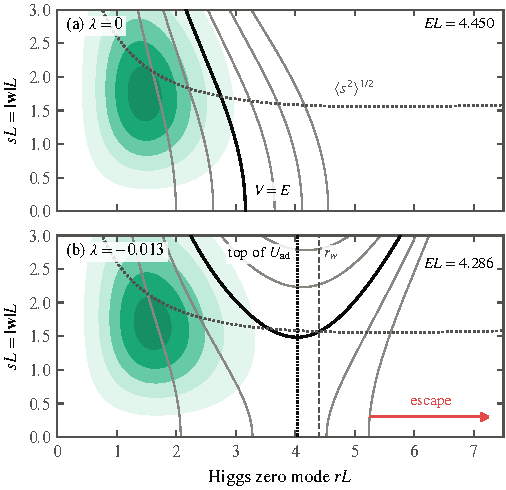
\includegraphics[width=0.7\textwidth]{prd_higgs_wavefunction}
\caption{Higgs and hypercharge zero modes in the two-dimensional model.
Filled contours: probability density of the lowest state in the $(r,s=|\bm w|)$ plane; thin lines: equipotentials of $V(r,s)$, the thick one at the eigenvalue $E$; dotted curve: transverse zero-point width $\langle s^2\rangle^{1/2}$.
(a)~$\lambda=0$: bound ground state.
(b)~$\lambda=-0.013$: quasi-bound state, computed with a wall at $r_w$ (dashed) beyond the top of the adiabatic barrier (dotted).
$V$ stays open at small $s$; the barrier comes from the zero-point energy of the gauge zero modes, and beyond its outer turning point the state escapes along $r$.} %
\label{fig:rb-wavefunction}
\end{figure}

\subsection{The finite-volume resonance as a multichannel Siegert state}
\label{sec:rb-siegert}

For $\lambda<0$ we solve $H_{\rm 2D}\psi=E\psi$ with complex $E=\varepsilon-i\Gamma/2$, where $\Gamma$ is the full width in conformal time (units $1/L$).
A Siegert state~\cite{Siegert:1939zz} is regular at the origin and purely outgoing at large $r$; it exists only at the discrete complex energies of the resonances, and $\Gamma$ is the decay rate of the quasi-stationary state.

\paragraph{Discretization and integration.}
In $s$ we use a sine discrete-variable representation on $(0,S_{\max})$, which builds in $v(0)=0$; in $r$ we integrate the matrix Numerov equation with renormalization.
We start at $r_0=0.01$ from the Frobenius solution $r^{s_0}(1+\alpha r/s_0)$, with $s_0=3/2$ for the two-dimensional model and $s_0=1.6726$ when $B_w\to3/(16r^2)$ is kept. %
At $R_{\rm out}=16$ we transform to the local adiabatic channels of $\bm w$, the eigenvectors of the $\bm w$ Hamiltonian at fixed $r$, and impose in each channel $m$ the outgoing (or, for closed channels, decaying) condition. %
For $u''+k^2(r)u=0$ the WKB solution $u\propto k^{-1/2}\exp(i\int^rk\,dr')[1+O(\hbar^2)]$ has the logarithmic derivative
\begin{equation}
\frac{u_m'}{u_m}=Y_m\equiv ik_m-\frac{k_m'}{2k_m}+\frac{i}{2k_m}\Bigl(\frac{3k_m'^2}{4k_m^2}-\frac{k_m''}{2k_m}\Bigr),
\label{eq:rb-siegert}
\end{equation}
to second order, with $k_m(r)=\{2[E-U_m(r)]\}^{1/2}$ and $U_m$ the adiabatic channel potential.
The resonance is a zero of the root function
\begin{equation}
f(E)=\det\bigl(u'_m-Y_mu_m\bigr),
\label{eq:rb-rootfn}
\end{equation}
evaluated on the matrix solution propagated from the origin.
We accumulate the determinant with a signed log-determinant, so that $f$ is an entire function of $E$, and we refine its zeros with Muller's method.

\paragraph{Locating the right zero.}
All channels are open in the outer region, so the phase of $f$ turns by about $N\,T_{\rm out}$ radians per unit energy, where $N$ is the number of channels and $T_{\rm out}$ the classical time in the outer region.
Muller iterations started with a wide step then converge onto Siegert zeros of box states of the $s$ direction, which move with $S_{\max}$, lie above the Born--Oppenheimer bracket, and have widths $0.7$--$1.3$. %
We therefore scan $|f|$ along the real axis in a window around the expected root, take the interior local minimum nearest the window centre, and start Muller there with a step of $0.001$. %
Every root is then recomputed with a larger $s$ box; a change $|\Delta E|>\max(2\times10^{-7},2\times10^{-3}\Gamma)$ flags a box state. %
This protocol is essential: an unguided search returns box zeros whose widths exceed the resonance width by orders of magnitude.

\begin{table}[t]
\centering
\caption{Static widths (units $1/L$) of the one-dimensional Born--Oppenheimer model, the two-dimensional model, and its Gaussian version 2D$_{\rm G}$, with the fixed couplings and the matching of Sec.~\ref{rep:h-matching}.} %
\label{tab:rb-widths}
\begin{tabular}{ccccc}
\toprule
$\lambda$ & $\Gamma_{\rm 1D}$ & $\Gamma_{\rm 2D}$ & $\Gamma_{\rm 2D}^{\rm G}$ & $\Gamma_{\rm 2D}/\Gamma_{\rm 1D}$ \\
\midrule
$-0.008$ & $2.010\times10^{-4}$ & $7.865\times10^{-5}$ & $1.032\times10^{-4}$ & $0.391$ \\ %
$-0.010$ & $9.871\times10^{-4}$ & $4.154\times10^{-4}$ & $5.318\times10^{-4}$ & $0.421$ \\ %
$-0.0143$ & $7.803\times10^{-3}$ & $3.774\times10^{-3}$ & $4.625\times10^{-3}$ & $0.484$ \\ %
\bottomrule
\end{tabular}
\end{table}

\paragraph{Convergence and independent methods.}
The widths converge fast (Table~\ref{tab:rb-widths}).
At $\lambda=-0.010$ and $-0.0143$, changing $(N,S_{\max})$ from $(32,14)$ to $(48,16)$ or $(24,12)$ changes $\Gamma$ by $2\times10^{-10}$, halving the step to $h=0.001$ by at most $8\times10^{-8}$, moving $R_{\rm out}$ to $14$ by $7\times10^{-7}$, and dropping the second-order terms of Eq.~(\ref{eq:rb-siegert}) by $3.4\times10^{-3}$, which measures the order of the outgoing condition. %
Three independent methods agree.
(i)~Finite differences with a complex absorbing potential (CAP) $-i\eta(r-7)^2\theta(r-7)$, with $\eta$ at the most stable point~\cite{Riss:1993cap}, give $\Gamma_{\rm 2D}/\Gamma_{\rm 1D,ex}=0.5313$ and $0.5317$ at grid steps $0.04$ and $0.03$, against $0.5303$ from the Siegert roots; the absolute CAP widths are low by $2.6\%$ in both models, which cancels in the ratio. %
In the final model the CAP pole agrees with the Siegert root to $0.08\%$ in $\Gamma$. %
(ii)~A real wall moved from $R_w=8$ to $11$ at $\lambda=-0.0143$ shows one level that stays at $\varepsilon=4.2737\pm0.002$ while the others cross it, matching the Siegert value $4.27375$. %
(iii)~For the one-dimensional model, exterior complex scaling~\cite{Simon:1979ecs} agrees with the Siegert root for the same inner boundary to $3\times10^{-9}$ in $E$ and $3\times10^{-7}$ relative in $\Gamma$. %
The CAP eigenvector has $P(r<5)=0.9988$ at $\lambda=-0.010$, and the probability beyond $0.75\,S_{\max}$ in $s$ is $10^{-10}$, so the resonance is localized in the well and the $s$ box plays no role. %

Two analytic limits check the solver.
A three-dimensional isotropic oscillator in the s wave gives $0.4500000000041$ against $0.45$ in a finite-element calculation, and the uncoupled limit $\Omega\equiv0.3$ separates to $8\times10^{-11}$. %
Over $\lambda=-0.004$ to $-0.020$ the Kemble WKB width agrees with the exact one to $3\%$ for tunneling exponents $S\approx2$--$25$. %
Changing the potential beyond $1.5$ times the outer turning point (linear tail, doubled quartic, frozen matching) changes $\Gamma$ by at most $0.75\%$, and beyond twice that radius by $10^{-4}$; the radial non-zero modes become tachyonic only at $r\approx31$. %

\paragraph{Mechanism.}
The resonance tunnels in $r$ through the barrier at $r\approx3$--$5.5$ while $\bm w$ stays in its local ground channel. %
At $\lambda=-0.010$ the resonance energy of the two-dimensional model lies $0.123/L$ below that of the one-dimensional model, $0.051$ from the gauge shape and $0.072$ from the $\bm w$ dynamics, while the barrier is unchanged. %
The width $\Gamma_{\rm 2D}=4.15\times10^{-4}$ lies between the Born--Oppenheimer values without and with $B_w$, $3.88\times10^{-4}$ and $7.99\times10^{-4}$, only $7\%$ above the first: nearly all of $B_w$ is spurious. %
The joint dynamics lowers the well and leaves the barrier unchanged, so that $\Gamma_{\rm 2D}/\Gamma_{\rm 1D}=0.39$--$0.48$ for $\lambda$ between $-0.008$ and $-0.0143$. %
The ratio decreases smoothly as $\lambda\to0^-$, because the barrier thickens and the same energy shift is amplified, and no $\lambda$-independent decay channel appears.

\paragraph{Inhomogeneous decay.}
Inhomogeneous decay is much slower than this homogeneous channel.
The scale-invariant instanton has action $8\pi^2/(3|\lambda|)\approx2.6\times10^3$ at $|\lambda|=0.01$~\cite{Andreassen:2017rzq}, compared with zero-mode tunneling exponents of $2$--$6$, and on the torus the non-zero modes turn tachyonic only far beyond the exit point. %

\subsection{Node-direct roots with running couplings}
\label{sec:rb-nodes}

For the hazard of Sec.~\ref{rep:h-survival} we solve the two-dimensional model directly at each node $\tau=0,0.5,\ldots,5$ of the turn and for each top mass on a grid of $0.2\GeV$. %
At each node we recompute the conditional Gaussian with the node couplings $g_2$ and $g_Y$, decompose it into $C_0$, $B_x$, and $\Omega_{\rm eff}^2$, evaluate $\Delta V_{\rm MC}$ with $(\lambda,g_2,g_Y,y_t)$ at $\mu(\tau)$, add the cross terms of Sec.~\ref{rep:h-cross}, and find the root.
No width ratio, interpolation in $\lambda$, or fitted correction enters.
The standard configuration is $N=24$, $S_{\max}=12$, $h=0.004$, $R_{\rm out}=16$. %
The root window is centred $0.0035$ below the root of the effective one-dimensional model at the same node, with half-width $0.012$ and scan step $0.0012$. %
In the runs with the earlier mapping all 377 two-dimensional columns passed the window and box tests at the first attempt, with $|\Delta E|\le1.4\times10^{-11}$ and relative changes of $\Gamma$ of at most $7.8\times10^{-5}$ under the box change, and the 220 columns of the run with the NNLO mapping passed in the same way. %
Relative to the configuration of Table~\ref{tab:rb-widths}, the standard configuration changes $\Gamma$ by at most $1.2\times10^{-6}$, $R_{\rm out}=14$ by $2.7\times10^{-6}$, and a zeroth-order outgoing condition by $3.0\times10^{-3}$; on the critical mass these are below $4\times10^{-7}$, $9\times10^{-7}$, and $1.0\times10^{-3}\GeV$. %
Eleven nodes instead of 29 change $m_c$ by $7\times10^{-5}\GeV$, and with the fixed couplings the node code reproduces the static widths of Table~\ref{tab:rb-widths} to $4.4\times10^{-6}$. %
These checks give the numerical item, $\pm0.002\GeV$, of the error budget (Sec.~\ref{rep:h-budget}); the full set of numerical controls is collected in Sec.~\ref{rep:v-convergence}. %

The two-dimensional model with the DMC shape was evaluated in three ways, by a ratio conversion of static widths, by an effective one-dimensional hazard, and by direct two-dimensional roots at every node; the last two change $m_c$ by only $0.011$ and $0.001\GeV$, so the numerical implementation of the reduced model has converged. %

\subsection{Full-dimensional validation and independent reimplementation: results}
\label{sec:rb-fulldim}

Section~\ref{rep:v-fulldim} describes the full-dimensional checks in detail; here we state the results that enter the error budget.
A Dirichlet wall at the gauge-invariant radius $|\bm\phi|=r_w$, between the barrier top and the outer classical turning point, is the only node of the walled ground state, so DMC for the full Hamiltonian in all sixteen coordinates has no fixed-node error.
The difference from the two-dimensional model with the same wall is $\Delta\varepsilon=-0.0032(8)$ at $\lambda=-0.010$ and $-0.0034(9)$ at $\lambda=-0.013$, independent of the wall position, and $-0.0043(9)$ at $\lambda=0$. %
The reduction error is thus a constant shift of the well by about $-0.0035/L$. %
With $d\ln\Gamma/d\varepsilon=7.6$ and $7.1$ from the two-dimensional model, $\Gamma_{\rm full}/\Gamma_{\rm 2D}=0.976$, and with the slopes $d\ln I/dm_t=5.269$, $3.218$, and $2.121\GeV^{-1}$ of the final hazard (Sec.~\ref{rep:h-survival}) %
\begin{equation}
\Delta m_c=-\frac{\ln(\Gamma_{\rm full}/\Gamma_{\rm 2D})}{d\ln I/dm_t}=+0.0046(11),\ +0.0075(19),\ +0.0115\GeV %
\label{eq:rb-dmc-conv}
\end{equation}
at $\Pone=0.9$, $1/2$, and $0.1$.
Three other estimates of the width ratio agree: multidimensional adiabatic WKB gives $0.937$ including $B_w$ under the barrier, the wall dependence of the tunneling tail gives $0.92(16)$ and $1.03(7)$, and a three-dimensional model with an SU(2) breathing mode gives $0.999$ (Fig.~\ref{fig:rb-gamma}). %
We carry the WKB envelope as a one-sided error, $+0.012$, $+0.020$, and $+0.031\GeV$ at $\Pone=0.9$, $0.5$, and $0.1$. %
Because $\Delta\varepsilon$ depends neither on the wall nor on $\lambda$, we apply the same ratio at every node and at $\Pone=0.1$, where $\lambda(\mub)=-0.0152$. %

The validation was done at fixed couplings and without the cross terms of Sec.~\ref{rep:h-cross}.
The cross terms stiffen the $\bm w$ direction and make it more adiabatic: the two-dimensional width exceeds that of the adiabatic one-dimensional reduction by only $1.0$--$1.8\%$ in the final model, against $6$--$8\%$ without cross terms, so the reduction is, if anything, more accurate in the final model. %
Within these assumptions the reduction moves the critical mass by at most $0.031\GeV$. %
An independent blind reimplementation of the chain without cross terms, with the earlier Standard Model mapping, reproduces its critical masses to $0.005\GeV$ (Sec.~\ref{rep:v-blind}). %

\begin{figure}[t]
\centering
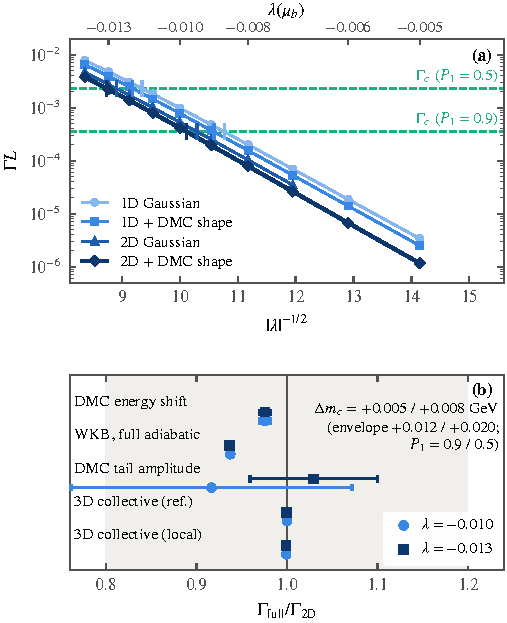
\includegraphics[width=0.66\textwidth]{prd_gamma_validation}
\caption{Resonance widths of the reduced models and their full-dimensional check.
(a)~$\Gamma L$ against $|\lambda|^{-1/2}$ for one- and two-dimensional models with Gaussian or DMC gauge shape; the straight lines on the logarithmic scale are the WKB form $\ln\Gamma=a-b|\lambda|^{-1/2}$.
Dashed: the constant widths $\Gamma_c=-\ln\Pone/\eta_\infty$ that give $\Pone=0.5$ and $0.9$; ticks: where each model reaches them.
(b)~$\Gamma_{\rm full}/\Gamma_{\rm 2D}$ at $\lambda=-0.010$ and $-0.013$ from four estimators; all lie within $20\%$ (band) and would raise $m_c$ by $+0.005$ and $+0.008\GeV$ at $\Pone=0.9$ and $0.5$, a shift not included in the central values (one-sided envelope $+0.012$ and $+0.020\GeV$).} %
\label{fig:rb-gamma}
\end{figure}

\subsection{The size of the threshold}
\label{sec:rb-size}

The threshold $\lamc\approx-0.01$ follows from three ingredients: the WKB form of the width, the duration of the turn, and the residual linear confinement after the matching.
Figure~\ref{fig:rb-threshold}(a) shows the effective potential along $r$ near threshold.

\paragraph{WKB exponent of a linearly confined quartic runaway.}
For $U(r)=\sigma r-|\lambda|r^4/4$ and an energy well below the barrier, the outer turning point is $r_0=(4\sigma/|\lambda|)^{1/3}$, and with $r=r_0x$ one has $U=\sigma r_0\,x(1-x^3)$.
The tunneling exponent is
\begin{equation}
S=2\int_0^{r_0}\!\sqrt{2U}\,dr=2\sqrt{2\sigma}\,r_0^{3/2}\int_0^1x^{1/2}(1-x^3)^{1/2}dx=\frac{2\pi\sqrt2}{3}\frac{\sigma}{|\lambda|^{1/2}}\simeq2.962\,\frac{\sigma}{|\lambda|^{1/2}}, %
\label{eq:rb-wkb}
\end{equation}
where the substitution $x^3=v$ turns the integral into $\frac13B(\frac12,\frac32)=\pi/6$ and $r_0^{3/2}=2\sigma^{1/2}|\lambda|^{-1/2}$.
The width therefore obeys $\ln\Gamma=a-b|\lambda|^{-1/2}$ with $b=2.962\,\sigma$. %
Fits to the nodal widths give $b=1.31$--$1.38$ (at $\tau=0$: $a=5.91$, $b=1.307$; the static box at $\mub$ gives $a=\aFitA$ and $b=\bFitA$ for $\lamFitLo\le\lambda\le\lamFitHi$, Sec.~\ref{sec:v11-static-box}), with root-mean-square residuals $0.05$--$0.09$ in $\ln\Gamma$; a three-parameter form $a-b|\lambda|^{-p}$ gives $p=0.74$ at $\tau=0$ and $0.55$ at $\tau=5$, because the local exponent flattens as the resonance approaches the barrier top. %

\paragraph{Hazard form.}
The hazard of Sec.~\ref{rep:h-survival} integrates $\Gamma$ over the conformal duration $\eta_\infty$ of one branch.
We define the effective exponent of the hazard by its logarithmic derivative at threshold,
\begin{equation}
b_{\rm eff}\equiv2|\lamc|^{3/2}\Bigl|\frac{d\ln I}{d\lambda(\mub)}\Bigr|=1.40,\ 1.30,\ 1.19 %
\label{eq:rb-beff}
\end{equation}
at $\Pone=0.9$, $0.5$, and $0.1$, from $d\ln I/d\lambda(\mub)=-805$, $-488$, and $-319$. %
Up to a slowly varying prefactor, $I\simeq A_{\rm eff}\,\eta_\infty\exp(-b_{\rm eff}|\lambda|^{-1/2})$, with $\lambda\equiv\lambda(\mub)$.
The effective slope $\sigma_{\rm eff}=b_{\rm eff}/2.962=0.44$ at $\Pone=1/2$ ($0.47$ and $0.40$ at $\Pone=0.9$ and $0.1$) is about one third of the zero-point slope $\sigma_0=1.31$ of Eq.~(\ref{eq:rb-linear}): in the reduced model the zero-point energy rises with slope $\zpSlopeLo$--$\zpSlopeHi$ rather than $\sigma_0$ at $r=1$--5 (Sec.~\ref{sec:v11-static-box}), the WKB form absorbs the finite height of the barrier, and the one-loop energy of the non-zero modes lowers the local slope by $10$--$33\%$ at $r=1$--5 and roughly halves the barrier above the resonance level, without removing the confinement. %
In the reduced model of Fig.~\ref{fig:rb-threshold}(a), without cross terms, and for the radial potential including the centrifugal term $3/(8r^2)$, the barrier above the resonance level falls from $1.565/L$ to $0.715/L$ for $\lambda=-0.010$ and from $1.211/L$ to $0.534/L$ for $\lambda=-0.013$ when the matching is included. %
The matching combines the destabilizing tadpole of the periodic bosons (Sec.~\ref{sec:rb-tower}) with the stabilizing one of the antiperiodic top tower (Sec.~\ref{sec:rb-rg}), and the hypercharge zero mode, pinned by the antiperiodic fermions (Sec.~\ref{rep:h-cross}), also enters $\sigma_{\rm eff}$. %

\paragraph{Closed form for the threshold.}
Setting $I=\ln2$ (that is, $\Pone=1/2$) gives
\begin{equation}
|\lamc|^{1/2}\simeq\frac{b_{\rm eff}}{\ln(A_{\rm eff}\,\eta_\infty/\ln2)} .
\label{eq:rb-lamc-size}
\end{equation}
The effective prefactor $A_{\rm eff}\simeq310$ absorbs the energy of the resonance ($\varepsilon\approx4.3/L$), the shape of the barrier, and the reduction of the width by the running along the turn; it is fixed by reproducing the computed threshold and is not universal. %
With $b_{\rm eff}=1.30$ and $\eta_\infty=299.8$, this value of $A_{\rm eff}$ returns $\lamc=-0.0121$ by construction; the content of the formula is the logarithmic dependence, checked directly in Sec.~\ref{rep:h-universality}. %
The running matters at the level of the effective duration: holding the $\tau=0$ width for the whole branch would overestimate the hazard, and $I/(\Gamma(0)\eta_\infty)=0.77$, $0.82$, and $0.87$ at the three levels. %
The duration and the prefactor enter only through the logarithm: doubling or halving $\eta_\infty$ changes $|\lamc|$ by $-11\%$ or $+13\%$, and changing $g_2$, $g_Y$, or $y_t$ by $10\%$ changes it by $6.6\%$, $1.6\%$, or $6.3\%$, so the magnitude $\lamc\approx-0.01$ is fixed to within a factor of about $1.2$. %
The effective exponent at threshold, $S_c=b_{\rm eff}/|\lamc|^{1/2}=14.7$, $11.8$, and $9.7$ at the three levels, is moderate, which is why the threshold is sharp in $\lambda$ but not in $\Pone$. %
It is the exponent of this effective law, whose prefactor $A_{\rm eff}\simeq310$ absorbs a factor of order $e^6$; the WKB barrier action is smaller, $4.3$ at the static threshold $\lamc(300)$ (Sec.~\ref{sec:v11-mechanism-context}). %
The dependence on the duration and on the couplings is worked out in Sec.~\ref{rep:h-universality}.

\begin{figure}[t]
\centering
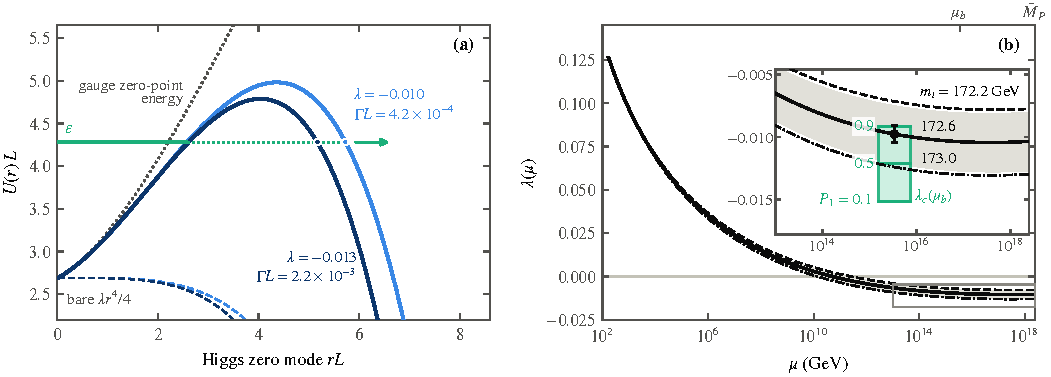
\includegraphics[width=\textwidth]{prd_threshold}
\caption{Finite-volume threshold of the Higgs zero mode.
(a)~Effective potential along $r$ for $\lambda=-0.010$ and $-0.013$ (reduced model without cross terms or centrifugal term): the zero-point energy of the gauge zero modes (dotted), lowered by the non-zero modes, holds back the negative quartic (dashed), so the state is a resonance at $\varepsilon$ with width $\Gamma$ (dots: outer turning points). %
(b)~Running quartic coupling $\lambda(\mu)$ for $m_t=172.2$ (dashed), $172.6$ (solid), and $173.0\GeV$ (dash-dotted), with the band from $\alpha_s(M_Z)=0.1180\pm0.0009$; inset: the hazard-equivalent threshold $\lamc(\mub)$ for $\Pone=0.9$, $0.5$, and $0.1$, and the Standard Model value with its mapping uncertainty (Sec.~\ref{rep:h-smmap}).} %
\label{fig:rb-threshold}
\end{figure}

\subsection{The confinement mechanism in field-theory context}
\label{sec:v11-mechanism-context}

The confinement of the Higgs zero mode rests on one term, the zero-point energy of the constant $W$ and $Z$ modes at fixed $r$, which grows linearly with $r$.
This subsection relates that term to known structures of small-volume gauge theory, matrix models and thermal field theory, states which fields can cancel it, and compares the resonance with the decay channels of a small compact space, with inhomogeneous tunnelling and with Planck-suppressed operators.
Numbers refer to the static box of Sec.~\ref{sec:v11-static-box}; its box~A has the Standard Model couplings at $\mu=\mub$ for $m_t=172.60\GeV$, which are those of the first node of the turn. %
The fit window is the range $\lamFitLo\le\lambda\le\lamFitHi$ in which Sec.~\ref{sec:v11-static-box} fits the widths of box~A with Eq.~(\ref{eq:rb-wkb}), and $\kappa$ is the factor by which Sec.~\ref{sec:v11-kappa} multiplies the couplings of the gauge zero modes. %

\paragraph{A linear term from the constant gauge modes.}
At fixed $r$ the mass matrix of Eq.~(\ref{eq:rb-massmatrix}) makes the constant $W$ and $Z$ modes oscillators of frequencies $g_2r/2$ and $g_Zr/2$, whose zero-point energy rises as $\sigma_0r$ with $\sigma_0=\frac32g_2+\frac34g_Z$ [Eq.~(\ref{eq:rb-linear})]; with the couplings of box~A, $\sigma_0=1.31$. %
Since $r=(2\Phi^\dagger\Phi)^{1/2}$, the term is linear in $|\Phi|$ and not analytic in $\Phi^\dagger\Phi$.
It plays the role of the zero-point energy along the classically flat valleys of a quartic potential.
At $\lambda=0$ the potential of Eq.~(\ref{eq:rb-H0}) vanishes along the whole Higgs direction $\bm x=\bm w=0$, and the zero-point energy of the transverse gauge modes closes this valley, as it makes the spectrum of $p_x^2+p_y^2+x^2y^2$ discrete although the classically allowed region extends to infinity along the axes~\cite{Simon:1983jy}.
In SU(2) Yang--Mills theory on a small torus the same mechanism gives an abelian constant mode $C$ the conical potential $2|C|/L$ (in the normalization of Ref.~\cite{vanBaal:2000zc}), the zero-point energy of the four charged constant modes of frequency $|C|/L$ transverse to it~\cite{vanBaal:2000zc,Barbon:2005zj}, and it makes the spectra of the bosonic membrane and of bosonic matrix models discrete~\cite{deWit:1988xki,Barbon:2005zj}. %
The Higgs zero mode differs from these examples in that its valley falls as $-|\lambda|r^4/4$ for $\lambda<0$, so the linear term holds the zero mode only up to the barrier at $r_{\rm top}=(\sigma/|\lambda|)^{1/3}$ (Sec.~\ref{sec:rb-H0}), and the bound state of the valley becomes the resonance of Sec.~\ref{sec:rb-siegert}.

\paragraph{Relation to the thermal cubic term.}
The linear term is the finite-volume counterpart, with the opposite sign, of the term cubic in the gauge-boson masses that the static Matsubara modes add to the effective potential at finite temperature~\cite{Dine:1992wr,Arnold:1992rz}.
Both terms come from bosonic modes that have no gap from the compact directions.
Such a mode of a real boson of mass $m$ is integrated only over its $d$ non-compact Euclidean directions, and in dimensional regularization
\begin{equation}
\frac12\int\!\frac{d^dk}{(2\pi)^d}\,\ln\bigl(k^2+m^2\bigr)=-\frac{\Gamma(-d/2)}{2\,(4\pi)^{d/2}}\,m^d
=\begin{cases}+\dfrac{m}{2}, & d=1,\\[8pt] -\dfrac{m^3}{12\pi}, & d=3,\end{cases}
\label{eq:v11-gapless}
\end{equation}
which follows from $\int d^dk\,(2\pi)^{-d}(k^2+m^2)^{-1}=\Gamma(1-d/2)\,m^{d-2}/(4\pi)^{d/2}$ by integration in $m^2$, with $\Gamma(-\frac12)=-2\sqrt\pi$ and $\Gamma(-\frac32)=\frac43\sqrt\pi$.
At temperature $T$ the free-energy density of the field is $T\sum_n\frac12\int d^3k\,(2\pi)^{-3}\ln(\omega_n^2+k^2+m^2)$ with $\omega_n=2\pi nT$.
The static mode $n=0$ is a three-dimensional field and contributes $-Tm^3/(12\pi)$, while the modes with $n\neq0$ have the gap $2\pi T$ and are analytic in $m^2$ for $|m|<2\pi T$~\cite{Dine:1992wr}.
In the box at zero temperature the energy is $\frac12\sum_{\bm k}\omega_{\bm k}=\sum_{\bm k}\frac12\int dk_0\,(2\pi)^{-1}\ln(k_0^2+\bm k^2+m^2)$.
The constant mode $\bm k=0$ is a quantum oscillator and contributes $+m/2$, while the modes with $\bm k\neq0$ have the gap $2\pi/L$ and give the energy $E_{\rm std}$ of Eq.~(\ref{eq:rb-Estd}), analytic in $m^2$ for $|m|<2\pi/L$.
For the electroweak gauge bosons the counting is the same in both cases, six $W$ and three $Z$ modes, from the three polarizations of each massive vector at finite temperature and from the three spatial directions of each constant mode in the box, so that
\begin{equation}
\Delta V_T\supset-\frac{T}{12\pi}\bigl(6m_W^3+3m_Z^3\bigr),\qquad
L\,\Delta E_{\rm box}=\frac L2\bigl(6m_W+3m_Z\bigr)=\sigma_0r,
\label{eq:v11-cubic-linear}
\end{equation}
with $m_W=g_2r/(2L)$ and $m_Z=g_Zr/(2L)$ in the box.
The first expression is the leading cubic term of the thermal potential, before the resummation of the static modes~\cite{Arnold:1992rz}, and the second is Eq.~(\ref{eq:rb-linear}).
The sign is that of $-\Gamma(-d/2)$, positive for $d=1$ and negative for $d=3$: the constant spatial modes are quantum oscillators with positive zero-point energy, whereas the one-loop energy of the three-dimensional static field is negative.
The roles differ accordingly: at finite temperature the negative cubic term produces the barrier of a first-order transition between the symmetric and the broken phase; in the box the positive linear term holds the zero mode at the origin against the negative quartic.

Terms proportional to $(m^2)^{d/2}$ with odd $d$ are non-analytic in $\Phi^\dagger\Phi$~\cite{Barbon:2006us}.
The infinite-volume effective potential at zero temperature contains no odd power of $m$: every mode is integrated over four non-compact directions, and the same integral gives, after $\MSbar$ subtraction, the Coleman--Weinberg term of Eq.~(\ref{eq:rb-VCW}), whose logarithm is the only non-analyticity of that potential.
For masses large compared with the gap the gapped modes cancel the non-analytic term again: in the box $D_P(m^2)\to-m/2+0.8375$ for $mL\gg2\pi$ (Sec.~\ref{sec:rb-tower}). %
Antiperiodic fermions have no mode without a gap, since their lowest momentum is $\sqrt3\,\pi/L$ in the box and $\pi T$ at finite temperature, so they give no such term; in the box they enter only through the matching potential, which is analytic in $\tilde m_t^2$ for $|\tilde m_t|<\sqrt3\,\pi/L$ (Sec.~\ref{sec:rb-tower}).

\paragraph{Constant fermion modes.}
Constant fermion modes act against the confinement.
If all three cycles of the torus are periodic, as for the torus of Ref.~\cite{Fornal:2026qfq}, every fermion has a constant mode at trivial holonomy; an SU(3) center holonomy twists the quarks by $\pm\frac13$ and removes their constant modes, and that sector is not analysed (Sec.~\ref{sec:rb-spin}). %
For the top quark at fixed $r$ its Hamiltonian is $\tilde m_t\,\psi_0^\dagger\gamma^0\psi_0$, summed over the three colours, with $\tilde m_t=y_tr/\sqrt2$ [Eq.~(\ref{eq:rb-masses})], and $\gamma^0$ has the eigenvalues $\pm1$, each twice degenerate.
In the charge-conjugation symmetric ordering each of the $4\times3$ levels of energy $\pm\tilde m_t$ contributes $-\tilde m_t/2$ to the ground-state energy, the filled negative levels through $\varepsilon/2$ and the empty positive ones through $-\varepsilon/2$, so that
\begin{equation}
E_t^{(0)}=-12\cdot\frac{\tilde m_t}{2}=-6\tilde m_t=-\frac{6y_t}{\sqrt2}\,r\simeq-1.82\,r,
\label{eq:v11-top-zero}
\end{equation}
with $y_t(\mub)=0.428$ of box~A. %
The factor $12$ is the weight with which the top quark enters the one-loop matching (Sec.~\ref{sec:rb-rg}).
The term exceeds $\sigma_0r=1.31\,r$, so the net linear term of the constant modes would be negative, $(1.31-1.82)\,r$, and the zero-point confinement would fail; the lighter fermions add terms smaller by their Yukawa couplings. %
This statement is qualitative: at large $r$ the non-zero modes of both towers cancel the constant-mode terms (Sec.~\ref{sec:rb-tower}), and at trivial holonomy the fully periodic torus does not turn around (Sec.~\ref{sec:rb-spin}).
It parallels the supermembrane, in which the fermionic zero-point energy cancels the bosonic one along the valleys and the spectrum becomes continuous~\cite{deWit:1988xki}.
With one antiperiodic cycle or more the fermions have no constant modes (Sec.~\ref{sec:rb-spin}), and nothing cancels the confinement by the gauge zero modes.

\paragraph{Uniform tunnelling in a small compact space.}
A small compact volume speeds up vacuum decay: when the volume is small, a uniform tunnelling mode replaces the bubble~\cite{Hassan:2026cmp}, and the Schwinger effect in small compact directions proceeds through a homogeneous channel~\cite{Brown:2015kgj}; thin-wall decay with one compact dimension has been analysed for a scalar field~\cite{Antoniadis:2024ent}.
These analyses treat a scalar field with a barrier of its own or the Schwinger discharge of an electric field; in none of them do gauge zero modes confine a scalar zero mode.
For the Higgs field at $\lambda<0$ the uniform mode has no barrier of its own.
With the couplings of the gauge zero modes switched off ($\kappa=0$ in Sec.~\ref{sec:v11-kappa}) its radial potential, $3/(8r^2)+\lambda r^4/4+\Delta V_{\rm MC}(r)$, falls monotonically for every $\lambda$ between $-0.04$ and $0$, and the zero mode has no narrow (quasi-bound) resonance. %
When space is a three-torus the gauge zero modes supply the barrier.
The decay of the electroweak state in the box is still much faster than bubble nucleation in infinite volume, as the next paragraph shows, but it is tunnelling with a finite width rather than a classical roll.

\paragraph{Inhomogeneous tunnelling.}
Section~\ref{sec:rb-siegert} compared the action of the scale-invariant bounce with the zero-mode tunnelling exponents $2$--$6$ of the earlier model.
In the static box at $\mub$ the WKB exponents across the barrier are $2.1$--$7.9$ in the fit window $\lamFitLo\le\lambda\le\lamFitHi$ of Sec.~\ref{sec:v11-static-box}, and $3.1$, $4.3$, $7.8$ and $12.5$ at the thresholds $\lamc(N)$ for $N=10^2$, $3\times10^2$, $10^4$ and $10^6$. %
The Fubini-type bounce of a negative quartic has the action $8\pi^2/(3|\lambda|)$ for every radius~\cite{Andreassen:2017rzq}, which is $1.8\times10^3$, $2.2\times10^3$, $3.7\times10^3$ and $5.9\times10^3$ at these thresholds, at least $450$ times the zero-mode exponent. %
For the Standard Model couplings, a bounce of radius $R<L$ probes $\lambda$ at scales above $1/L$, where $\lambda(\mu)\ge-0.0104$ for $m_t=172.6\GeV$, with the minimum near $4\times10^{17}\GeV$; its action is therefore at least $2.5\times10^3$, and at least $2.0\times10^3$ for $m_t=173.0\GeV$. %
Inhomogeneous decay is therefore negligible against the zero-mode channel for every duration considered here.

\paragraph{Planck-suppressed operators.}
The width depends on the potential only up to the outer turning point of the barrier, $r_{\rm out}=5.3$--$5.7$ in box~A for $\lamc(300)\le\lambda\le\lambda_{\rm SM}(\mub)$ and $6.4$ at $\lamc(10^4)$, that is, on field values $r\lesssim6$, or $\phi=r/L\lesssim0.008\,\MPbar$ at $\mub=\MPbar/722$. %
A term $c\,\phi^6/\MPbar^2$ in the potential adds $c\,r^6(\mu/\MPbar)^2$ to $LH$ at $\mu=1/L$, which acts as a shift of the quartic coupling by $\Delta\lambda_{\rm eff}(r)=4c\,r^2(\mu/\MPbar)^2$.
At $\mub$ and $r=6$ this is $2.8\times10^{-4}c$ ($2.2\times10^{-4}c$ and $2.5\times10^{-4}c$ at $r=5.3$ and $5.7$). %
Through $d\lambda(\mub)/dm_t\approx-0.0066\GeV^{-1}$ (Sec.~\ref{rep:h-smmap}) it raises the critical top mass by at most about $0.04c\GeV$ for $c>0$, which is below the Standard Model error of the criterion, $\pm0.10\GeV$, for $|c|\lesssim2$. %
Higgs-coupled states of mass $M$ between $2\pi\mub$ and $\MPbar$ would generate the same operator with $\MPbar$ replaced by $M$, which shifts the critical mass by about $0.042c\,(\MPbar/M)^2\GeV$; the magnitude of this shift stays below $0.10\GeV$ only for $M\gtrsim0.65\,|c|^{1/2}\MPbar$, so the criterion also assumes that such states, if present, lie near $\MPbar$ or couple weakly to the Higgs field. %

\section{Higgs zero mode III: cross terms with the nonzero modes}\label{rep:h-cross}

The gauge zero modes act on the non-zero modes of every charged field as constant connections, so the one-loop energy of Sec.~\ref{rep:h-matching} depends jointly on the Higgs radius $r$ and on the holonomies $(\bm x,\bm w)$.
Including all Standard Model fields, we find that these cross terms lower the critical top mass by $0.080$, $0.118$, and $0.160\GeV$ at $\Pone=0.9$, $1/2$, and $0.1$, with a model-internal error of $\pm0.008$, $\pm0.010$, and $\pm0.013\GeV$. %
We show that the antiperiodic fermions pin the hypercharge holonomy for every $r$, so that no instability of the soft $\bm w$ direction occurs; that the net sign comes from a hypercharge curvature that is nearly independent of $r$ while the tree-level stiffness of $\bm w$ grows with $r$; and that the one-loop logarithms of the Higgs--gauge-zero-mode terms close on the Higgs anomalous dimension (Sec.~\ref{sec:rb-r2c2}).
A blind calculation of the charged-component part, which carries all but $+0.005$ to $+0.007\GeV$ of the shift, gives $-0.081$, $-0.117$, and $-0.157\GeV$, against $-0.085$, $-0.124$, and $-0.167\GeV$ for the same part in our calculation; we keep the difference as an error (Sec.~\ref{rep:v-blind}). %

\subsection{Twisted sums and holonomy curvatures}
\label{sec:rb-twist}

We use the connection $D=\partial-i(A^aT_a+YB)$ with ${\rm tr}\,T_aT_b=\frac12\delta_{ab}$ and the constant modes $c=g_2\bm x$ and $u=g_Y\bm w$ in coordinates of unit period.
A field of charge $q$ in a constant background $\phi$ obeys $\psi(\bm x+\bm e_i)=e^{iq\phi_i}\psi(\bm x)$ after the background is gauged away, which is a twist of its boundary condition by $\bm\vartheta=q\bm\phi/2\pi$.
For one real degree of freedom of mass $m$ the finite-volume energy with twist $\bm\vartheta$ is the image sum of Eq.~(\ref{eq:rb-Etheta}), and its curvature at $\bm\vartheta=0$, the same in every direction by cubic symmetry, is
\begin{equation}
C(m)=\frac{\partial^2E_\vartheta}{\partial\vartheta_i^2}\Big|_0=\frac13m^2\sum_{\bm n\neq0}K_2(m|\bm n|)\times\begin{cases}1&\text{periodic},\\(-1)^{n_1+n_2+n_3}&\text{antiperiodic}.\end{cases}
\label{eq:rb-curv}
\end{equation}
Each real degree of freedom with statistics sign $s$ ($+1$ for bosons, $-1$ for fermions) and charge $q$ then contributes $s\,q^2C(m)/(4\pi^2)$ to the curvature of the one-loop energy in the holonomy $\phi$ [Fig.~\ref{fig:rb-diagrams}(e)].
For periodic fields the momentum mode $\bm k=0$ is a slow coordinate that belongs to the zero-mode dynamics, and we remove its contribution $2\pi^2/m$.
A direct mode sum, valid also for $m^2<0$, gives
\begin{equation}
C(m^2)=\tfrac23Z_1+2\pi^2\sum_{\bm k}{}'\Bigl[\frac{3m^2+2k^2}{3\omega^3}-\frac{2}{3k}\Bigr]+\frac{m^2}{6},
\label{eq:rb-curv-direct}
\end{equation}
where $\omega^2=k^2+m^2$ and $Z_1$ is $Z_P$ or $Z_A$ of Eq.~(\ref{eq:rb-tadpole}).
The summand is the direction-averaged second derivative of $\omega(\bm k-q\bm\phi)$, from which the massless value is subtracted; by Eq.~(\ref{eq:rb-noLog}) it falls as $k^{-5}$, so the curvature has no $\MSbar$ logarithm.
The last term is the difference between the cubic average on the lattice and the $d$-dimensional angular average of the continuum subtraction.
Hence $C=\frac23Z_1+m^2/6+O(m^4)$, and the two representations agree to $10^{-8}$--$10^{-10}$ for $m\ge0.6$; an independent Wolfram calculation with lattice shell sums agrees to $10^{-12}$. %

\paragraph{Curvatures at $r=0$.}
At $r=0$ all fields are massless and $C=\frac23Z_1$, so the curvature of a gauge factor is $\kappa=\sum s\,q^2Z_1/(6\pi^2)$ summed over its charged real degrees of freedom.
Counting the weights, for SU(3) the gluons contribute two polarizations times $2\cdot1^2+4\cdot(\frac12)^2$, a weight $6$, and the six quark flavors $4\times\frac12=2$ each; for SU(2) the $W$ bosons contribute $4$, the Higgs doublet $1$, and each of the twelve Weyl doublets $1$; for hypercharge the Higgs doublet contributes $1$ and the fermions $2\sum Y^2=20$, with $\sum Y^2=10/3$ per generation.
With the periodic bosons and antiperiodic fermions,
\begin{equation}
\kappa_3=\frac{6Z_P-12Z_A}{6\pi^2}=\frac{Z_P-2Z_A}{\pi^2},\qquad \kappa_2=\frac{5Z_P-12Z_A}{6\pi^2},\qquad
\kappa_Y=\frac{Z_P-20Z_A}{6\pi^2},
\label{eq:rb-kappas}
\end{equation}
where $Z_P=-8.913633$ and $Z_A=-2.519356$. %
Numerically $\kappa_3=-0.393$, $\kappa_2=-0.242$, and $\kappa_Y=+0.700$ (Sec.~\ref{rep:zeromodes}), and $\kappa_3/2$ reproduces the small-volume coefficient $-0.19631$ of Ref.~\cite{vanBaal:1988va}. %
With $\langle c^2\rangle=3.66$, $1.40$, and $0.82$ for the summed Gaussian widths of the SU(3), SU(2), and hypercharge zero modes, the first-order shift of the gauge ground state is %
\begin{equation}
\Delta Q=\tfrac12\kappa\langle c^2\rangle=-0.718-0.169+0.287=-0.601,
\label{eq:rb-DQ}
\end{equation}
as in Sec.~\ref{rep:zeromodes}. %
The hypercharge curvature is positive because the antiperiodic fermions pin the holonomy at its trivial value~\cite{vanBaal:1988va}: their weight exceeds that of the periodic Higgs doublet by $-20Z_A/|Z_P|=5.65$. %

\subsection{Cross terms at finite Higgs radius}
\label{sec:rb-hessian}

At $r>0$ the electroweak non-zero modes acquire the masses of Eq.~(\ref{eq:rb-masses}), and each real degree of freedom contributes with its own mass and charge.
In the body frame the vev component has $T^3=+\frac12$ and $Y=\frac12$ (the rotation $\bm N\to\bm e_3$ puts the vev in the upper component, so the unbroken generator is $T^3-Y$), and the background is the Cartan direction $g_2x^3T^3+g_YwY$.
We use a charged-component approximation (CCA):
\begin{itemize}
\item the transverse $W$ modes count four with $|T^3|=1$ and $m^2=a_W$;
\item each Coulomb mode carries the charge of its Goldstone boson with $m^2=a+b$, which equals $\omega_C^2$ of Eq.~(\ref{eq:rb-coulomb}) up to $O(ab/k^2)$;
\item the radial mode has $m^2=3\lambda r^2$;
\item the two top chiralities decouple, with $\tilde m_t$ as a vectorlike mass;
\item the light fermions are massless.
\end{itemize}
In the SU(2) direction transverse to the background the $W$ modes contribute two polarizations times $C(a_W)+c_W^2C(a_Z)+s_W^2C(0)$, where $c_W$ and $s_W$ are the cosine and sine of the weak mixing angle.
This gives a holonomy Hessian $H(r)$ in the components $(x^1,x^3,w)$.
The approximations of the CCA along the broken direction are removed in Sec.~\ref{sec:rb-r2c2} and in Sec.~\ref{sec:rb-xfinal} below.

\paragraph{Average over the conditional Gaussian.}
In the conditional Gaussian of Eq.~(\ref{eq:rb-condGauss}), $x^3=-\beta w+\delta x^3$ with $\langle(\delta x^3)^2\rangle=1/(2k)$ and $\langle(x^{1,2})^2\rangle=1/(2a)$ per direction.
Averaging $\frac12y^{\mathsf T}Hy$ over the SU(2) modes and summing over the three directions gives
\begin{equation}
E_X(r,\bm w)=E_X^x(r)+\tfrac12\Omega_X^2(r)|\bm w|^2,\qquad
E_X^x=\frac{3H_{11}}{2a}+\frac{3H_{33}}{4k},\qquad
\Omega_X^2=H_{ww}-2\beta H_{3w}+\beta^2H_{33},
\label{eq:rb-EX}
\end{equation}
where the first term comes from two charged components with $\langle(x^{1,2})^2\rangle=1/(2a)$ in three directions, the second from $\delta x^3$, and $\Omega_X^2$ from substituting $x^3=-\beta w$ in the $(x^3,w)$ block.
$E_X^x$ adds to the radial potential $U_1$ and $\Omega_X^2$ to the stiffness of the $\bm w$ channel of Eq.~(\ref{eq:rb-H2D}).

\paragraph{SU(3)--top term.}
The gluon zero modes commute with the Higgs field, so their curvature is exact at quadratic order,
\begin{equation}
\kappa_3(r)=\frac{6C_P(0)-2\bigl[5C_A(0)+C_A(\tilde m_t^2)\bigr]}{4\pi^2},
\label{eq:rb-kappa3}
\end{equation}
since only the top quark among the six flavors is massive at $\mub$.
The gluon zero modes add $\Delta U_3=\frac12[\kappa_3(r)-\kappa_3(0)]\langle c^2\rangle_3$ to the radial potential.
With $C_A(\tilde m_t^2)-C_A(0)=\tilde m_t^2/6+O(\tilde m_t^4)$ this is, at small $r$, a negative Higgs mass term,
\begin{equation}
\Delta U_3\simeq-\frac{\langle c^2\rangle_3\,\tilde m_t^2}{24\pi^2}=\tfrac12\delta m^2r^2,\qquad
\delta m^2=-\frac{\langle c^2\rangle_3\,y_t^2}{24\pi^2}=-0.0032/L^2
\label{eq:rb-dm2}
\end{equation}
at the fixed couplings ($-0.0028/L^2$ with $y_t(\mub)$). %
Physically, the top quark stiffens the gluon holonomy at small $r$ and decouples at large $r$.

\begin{table}[t]
\centering
\caption{Cross-term coefficients of the fixed-coupling estimate at $\lambda=-0.008$: the SU(2) part $E_X^x$ and its split into $W$, Higgs-doublet, top, and light-fermion loops, and the hypercharge curvature $\Omega_X^2$ (units $1/L$).
The dependence on $\lambda$ enters only through the radial and Goldstone masses and is below $10^{-3}$.} %
\label{tab:rb-hessian}
\begin{tabular}{ccccccc}
\toprule
$r$ & $E_X^x$ & $W$ & $H$ & $t$ & light & $\Omega_X^2$ \\
\midrule
$1$ & $-0.177$ & $-0.442$ & $-0.110$ & $+0.046$ & $+0.328$ & $0.136$ \\ %
$2$ & $-0.160$ & $-0.401$ & $-0.100$ & $+0.041$ & $+0.300$ & $0.135$ \\ %
$3$ & $-0.139$ & $-0.348$ & $-0.087$ & $+0.034$ & $+0.263$ & $0.131$ \\ %
$5$ & $-0.099$ & $-0.253$ & $-0.064$ & $+0.022$ & $+0.197$ & $0.118$ \\ %
\bottomrule
\end{tabular}
\end{table}

Table~\ref{tab:rb-hessian} gives the coefficients.
The hypercharge curvature stays positive for all $r\in[0,8]$, falling from $0.137$ to $0.105$; at $r=1$ the light fermions give $+0.142$, the top quark $+0.023$, the Higgs doublet $-0.029$, and the $W$ bosons through the photon content of $\beta$ only $-3\times10^{-5}$. %
It equals $+0.137$ for $r\le1.5$ and $+0.118$ at $r=5$. %
Keeping only the Higgs doublet gives $\Omega_X^2=-0.029$ for $r\le2$ and an inverted $\bm w$ direction for $r<0.776$; with all fields this apparent instability of the soft $\bm w$ direction is absent. %
The SU(2) curvature is negative, with the $W$ loop ($-0.60$) and the Higgs doublet ($-0.15$) outweighing the left-handed fermions ($+0.51$) in units of $c$. %
The masses decouple the periodic fields by only a few percent, since $C_P(m)$ changes by at most $5\%$, while the antiperiodic top decouples by about $26\%$ at $r=5$; the dependence on $r$ comes mainly from the zero-mode widths. %
Keeping only the Higgs fluctuations reproduces the earlier estimates of the matching study pointwise, which fixes the normalization. %

\paragraph{Light-fermion twist energy, exact in $s$.}
The light-fermion part of the hypercharge dependence is large, and we treat it exactly in $s=|\bm w|$.
For the s wave the twist energy of the massless antiperiodic fermions, averaged over the direction of $\bm w$, is
\begin{align}
V_L(r,s)&=-2\sum_\alpha n_\alpha\Bigl[\bar E_A\Bigl(\frac{|q_\alpha|s}{2\pi}\Bigr)-\bar E_A(0)\Bigr],\nonumber\\
\bar E_A(t)&=-\frac{1}{2\pi^2}\sum_{\bm n\neq0}\frac{(-1)^{|\bm n|^2}j_0(2\pi|\bm n|t)}{|\bm n|^4},
\label{eq:rb-VL}
\end{align}
where $n_\alpha$ counts the light Weyl fermions with charge $q_\alpha=g_YY-g_2\beta T^3$ along $\bm w$, $j_0$ is the spherical Bessel function from the angular average of $\cos(2\pi\bm n\cdot\bm\vartheta)$, and $(-1)^{|\bm n|^2}=(-1)^{n_1+n_2+n_3}$.
It rises monotonically and stays bounded over the whole $s$ box, so no instability appears at higher order.
The modes $\bm n=0$ and $\bm n=-1$ of a periodic field become degenerate at $|\vartheta|=\frac12$, which lies at $s\ge7.5$, while the two-dimensional wave function has probability below $10^{-8}$ at $s>6$; restricting to the fundamental domain therefore changes nothing. %
The $W$, Higgs, and top parts of $\Omega_X^2$ are kept to quadratic order.

\subsection{Variational treatment and the fixed-coupling estimate}
\label{sec:rb-var}

In a first estimate we add the cross terms at fixed couplings in two ways.
The first-order version adds $E_X^x+\Delta U_3$ to the radial potential and $\frac12\Omega_X^2s^2+V_L$ to the $\bm w$ channel.
The variational version adds the Gaussian average of the Hessian,
\begin{equation}
F=\frac{3H_{11}}{2a}+\frac34\,\frac{H_{33}e-2H_{3w}c+H_{ww}k}{D},
\label{eq:rb-F}
\end{equation}
to the Gaussian functional of Eq.~(\ref{eq:rb-moments}), minimizes again at every $r$, and rebuilds $C_0$, $B_x$, $\beta$, and $\Omega_{\rm eff}^2$ from the new parameters; this lowers $a$ by $3\%$.
For SU(3) we minimize $E(s)=\alpha/s+\beta_3s^2+\kappa_3(r)s/2$ over the summed width $s=\langle c^2\rangle_3$, with $\alpha$ and $\beta_3$ fixed by the Gaussian ground state ($E_0=8.603$, $s_0=3.66$); the curvature increases $s$ to $3.819$ and the SU(3) term by a factor $1.044$. %
The roots are found as in Sec.~\ref{sec:rb-siegert}; all 49 resonances converge inside their windows. %

\begin{table}[t]
\centering
\caption{Ratio of the static width with cross terms to the width of the two-dimensional model, in the fixed-coupling estimate (variational treatment), for all terms together and for each group of fields alone.} %
\label{tab:rb-ratios}
\begin{tabular}{ccccc}
\toprule
$\lambda$ & All & SU(3)--top & SU(2) & U(1)$_Y$ \\
\midrule
$-0.008$ & $1.629$ & $1.218$ & $0.645$ & $2.057$ \\ %
$-0.010$ & $1.566$ & $1.179$ & $0.682$ & $1.932$ \\ %
$-0.0143$ & $1.456$ & $1.124$ & $0.744$ & $1.720$ \\ %
\bottomrule
\end{tabular}
\end{table}

Table~\ref{tab:rb-ratios} shows that the hypercharge part dominates and increases the width, the SU(3)--top part also increases it, and the SU(2) part decreases it.
At $\lambda=0$ the cross terms shift the ground state by $+0.064$: $+0.238$ from hypercharge, which narrows $\langle s^2\rangle$ from $4.47$ to $2.98$, $-0.170$ from SU(2), and $-0.005$ from SU(3)--top. %
Converted with the hazard slopes, the fixed-coupling estimate moves the critical mass by $-0.093$, $-0.135$, and $-0.180\GeV$ at $\Pone=0.9$, $0.5$, and $0.1$. %
The groups alone give $-0.137$, $-0.196$, and $-0.258\GeV$ (U(1)$_Y$), $-0.035$, $-0.044$, and $-0.055\GeV$ (SU(3)--top), and $+0.080$, $+0.108$, and $+0.139\GeV$ (SU(2)); their sum differs from the joint result by at most $0.007\GeV$, and the first-order and variational versions differ by at most $0.003\GeV$. %
At $\Pone=1/2$ the three groups, taken one at a time, are about $-0.20$, $-0.04$, and $+0.11\GeV$, and their sum agrees with the joint result of this estimate to $0.004\GeV$. %

\subsection{Mechanism}
\label{sec:rb-xmech}

The sign of the total has a simple origin [Fig.~\ref{fig:rb-cross}(a)].
The hypercharge curvature $\Omega_X^2$ is nearly independent of $r$, while the tree-level stiffness of the $\bm w$ mode grows with $r$ ($\Omega_{\rm eff}\simeq g_Yr/2$ at small $r$).
The zero-point energy that the curvature adds to the $\bm w$ oscillator,
\begin{equation}
\delta E_w=\tfrac32\Bigl[\bigl(\Omega_{\rm eff}^2+\Omega_X^2\bigr)^{1/2}-\Omega_{\rm eff}\Bigr],
\label{eq:rb-dEw}
\end{equation}
is therefore larger in the well, $0.24$--$0.32/L$ at $r\approx1$--$1.5$, than at the barrier, $0.13$--$0.17/L$ at $r\approx3$--$5$. %
It lifts $\varepsilon$ toward the barrier top and increases $\Gamma$.
The top quark stiffens the gluon holonomy at small $r$ and decouples at large $r$, which acts like the negative Higgs mass term of Eq.~(\ref{eq:rb-dm2}) and also increases $\Gamma$.
The SU(2) curvature is negative and lowers the well more than the barrier, which decreases $\Gamma$.
The net effect is destabilizing: the cross terms lower the critical top mass.

\subsection{Node-direct cross terms with running couplings}
\label{sec:rb-xdirect}

The main calculation adds the cross terms at every node of the hazard with the node couplings $(g_2,g_Y,y_t,\lambda,g_3)$ and the NNLO mapping of Sec.~\ref{rep:h-smmap}.
At each node and for each $(m_t,\alpha_s)$ we
(i)~recompute the Hessian;
(ii)~minimize the Gaussian functional with $F$ again, starting from the optimum without cross terms (to $|\nabla|<10^{-8}$ for $r>0.05$);
(iii)~add the increments of $C_0$, $B_x$, and $\Omega_{\rm eff}^2$, computed with one discretization, to the baseline profile;
(iv)~add $\Omega_X^2$ and $V_L$ to the $\bm w$ channel and the SU(3)--top term with $E_0=12.98\,g_3^{2/3}$ and $s_0=3.66\,(g_3/0.5396)^{2/3}$; and
(v)~solve for the two-dimensional root. %
The summed SU(3) width scales as $g_3^{4/3}$ rather than $g_3^{2/3}$ (with $x=g^{-1/3}y$ the zero-mode Hamiltonian is $g^{2/3}$ times a $g$-independent one, so $\langle c^2\rangle=g^2\langle x^2\rangle\propto g^{4/3}$); with the node couplings the power used changes $s_0$ by less than $1\%$ where the hazard accumulates ($\tau\lesssim1.5$), which moves the SU(3)--top part by at most $4\times10^{-4}\GeV$, inside its width item in Table~\ref{tab:rb-xerr}. %
Without cross terms this code path reproduces the baseline roots to $1.3\times10^{-13}$ in $\varepsilon$ and $5\times10^{-12}$ relative in $\Gamma$. %
All 220 columns (ten masses at $\alpha_s=0.1180$ and five at each of $0.1171$ and $0.1189$, eleven nodes each) converge without flags in every run. %
The width ratio at the nodes is $1.53$ at $\tau=0$ and $1.57$ at $\tau=5$ for $m_t=172.6\GeV$, two to three percent below the fixed-coupling estimate because the node Yukawa coupling is smaller. %
The direct shifts are about $9\%$ smaller than the fixed-coupling conversion, which they replace. %

The numerics of the roots with cross terms were checked at $m_t=172.4$, $172.6$, $173.0$, and $173.4\GeV$ and at $\tau=0$, $2.5$, and $5$. %
A larger box, the base configuration of Table~\ref{tab:rb-widths}, a halved step, and $R_{\rm out}=14$ change $\Gamma$ by at most $6\times10^{-6}$ relative and $m_c$ by at most $3\times10^{-6}\GeV$; a zeroth-order outgoing condition changes $m_c$ by $-0.0003$, $-0.0002$, and $-0.0013\GeV$, so we take $0.001\GeV$ as the numerical error. %
Replacing the CCA average by the exact second-order curvature of the mixed mass bubbles,
\begin{equation}
q^2\sum_{\bm k}{}'\Bigl[\frac{1}{2\omega_1}+\frac{1}{2\omega_2}-\frac{2k_i^2}{\omega_1\omega_2(\omega_1+\omega_2)}\Bigr],
\label{eq:rb-mixedbubble}
\end{equation}
which for $\omega_1=\omega_2$ reduces to the CCA summand and differs from it by terms of order $k^{-5}$ otherwise, changes $m_c$ by at most $0.0005\GeV$. %

\subsection{Final result, decomposition, and errors}
\label{sec:rb-xfinal}

The CCA misses three one-loop terms of order $r^2c^2$ along the broken direction, derived in Sec.~\ref{sec:rb-r2c2}: the transverse vev mixing through the vertex $2(c\Phi_0)^\dagger V\delta\Phi$ of background-covariant Coulomb gauge, the Coulomb mismatch, and the exact top chiral loop.
With all three added at every node before the variational minimization, the critical masses are $172.502$, $172.960$, and $173.418\GeV$ at $\alpha_s(M_Z)=0.1180$, $0.080$, $0.118$, and $0.160\GeV$ below the two-dimensional model without cross terms. %
Relative to the CCA result ($172.498$, $172.954$, $173.412\GeV$) the gauge part shifts $m_c$ by $+0.021$, $+0.028$, and $+0.034\GeV$ and the top chiral loop by $-0.017$, $-0.022$, and $-0.027\GeV$, a net $+0.005$, $+0.006$, and $+0.007\GeV$; the cancellation reflects $\gamma_\phi^C\approx2\times10^{-4}$. %
The same shifts appear at $\alpha_s=0.1171$ and $0.1189$, where the final critical masses are $172.156$, $172.611$, $173.069\GeV$ and $172.849$, $173.308$, $173.768\GeV$. %

In the final model we also removed groups of terms at every node in two orders.
The SU(3)--top part is $-0.031$, $-0.039$, and $-0.046\GeV$ when removed first and $-0.032$, $-0.040$, and $-0.048\GeV$ when removed last, nearly independent of the order. %
The hypercharge and SU(2) parts together give $-0.048$, $-0.078$, and $-0.112\GeV$, close to the sum of their fixed-coupling values at $\Pone=1/2$, $-0.09\GeV$. %
The vev-mixing-plus-Coulomb and top-chiral groups give $+0.0214$, $+0.0275$, $+0.0336\GeV$ and $-0.0168$, $-0.0219$, $-0.0270\GeV$, and their sum reproduces the difference between the final and the CCA results to $2\times10^{-4}\GeV$. %
We quote the hypercharge and SU(2) parts together, with their separate sizes from the fixed-coupling estimate of Sec.~\ref{sec:rb-var}, because the root search did not converge in windows of $\pm0.02$ and $\pm0.10$ when either was removed alone in the final model; we did not establish whether the resonance left the windows or a box zero was selected. %

\begin{table}[t]
\centering
\caption{Model-internal error of the cross-term shift of $m_c$ (GeV) in the final model, combined in quadrature.} %
\label{tab:rb-xerr}
\begin{tabular}{p{0.52\textwidth}ccc}
\toprule
Item & $\Pone=0.9$ & $0.5$ & $0.1$ \\
\midrule
SU(2) and SU(3) widths, CCA, direction averaging, first order versus variational & $0.008$ & $0.010$ & $0.013$ \\ %
RG-closure residual & $0.0006$ & $0.0008$ & $0.0010$ \\ %
Custodial ratio for the $W$ Coulomb term & $0.0010$ & $0.0013$ & $0.0015$ \\ %
Neutral Coulomb fit, top numerics & $0.0003$ & $0.0003$ & $0.0004$ \\ %
Numerics & $0.001$ & $0.001$ & $0.001$ \\ %
\midrule
Total & $\pm0.008$ & $\pm0.010$ & $\pm0.013$ \\ %
\bottomrule
\end{tabular}
\end{table}

Table~\ref{tab:rb-xerr} lists the model-internal error.
Its first row collects the width of the SU(2) Gaussian (taken as $10\%$ of the SU(2) part), the charged-component approximation, the SU(3) width (Gaussian $3.66$ against virial $3.77$), direction averaging, and the difference between the first-order and variational treatments, scaled by the ratio $0.91$ of direct to fixed-coupling shifts. %
The RG-closure residual is at most $3\%$ of the gauge part and also covers the residual of a consistent scale variation; the custodial item is the $25\%$ uncertainty of the $W$-direction Coulomb term (Sec.~\ref{sec:rb-r2c2}). %
The conditions are those of the reduced model, together with the CCA for the electroweak Hessian, the quadratic treatment of the $W$, Higgs, and top parts of the hypercharge dependence, and the Gaussian width of the gluon zero modes.

The blind calculation of the CCA part (Sec.~\ref{rep:v-blind}), written from the model definitions for the Gaussian two-dimensional model with the earlier mapping and a twisted-sum approximation, gives $-0.081$, $-0.117$, and $-0.157\GeV$ against $-0.085$, $-0.124$, and $-0.167\GeV$ in the main calculation. %
Its groups, $-0.126$, $-0.179$, and $-0.237\GeV$ (U(1)$_Y$), $-0.031$, $-0.039$, and $-0.047\GeV$ (SU(3)--top), and $+0.082$, $+0.109$, and $+0.136\GeV$ (SU(2)), agree with the fixed-coupling estimate to within $0.022\GeV$, that is, to $9\%$ for the hypercharge and SU(2) parts and to $15\%$ for the smaller SU(3)--top part. %
We keep the difference, $\pm0.004$, $\pm0.007$, and $\pm0.010\GeV$, as a separate systematic error in the budget; it may overlap partly with the first-order-versus-variational item above, which errs on the conservative side. %
The vev mixing, the Coulomb mismatch, and the top chiral loop, which together move $m_c$ by $+0.005$ to $+0.007\GeV$, are checked within the main code by the RG closure, the exact top logarithm, and the additivity of the groups. %
Two-loop cross terms, such as the QCD correction to the top loop on the gluon holonomy, are not computed.

\begin{figure}[t]
\centering
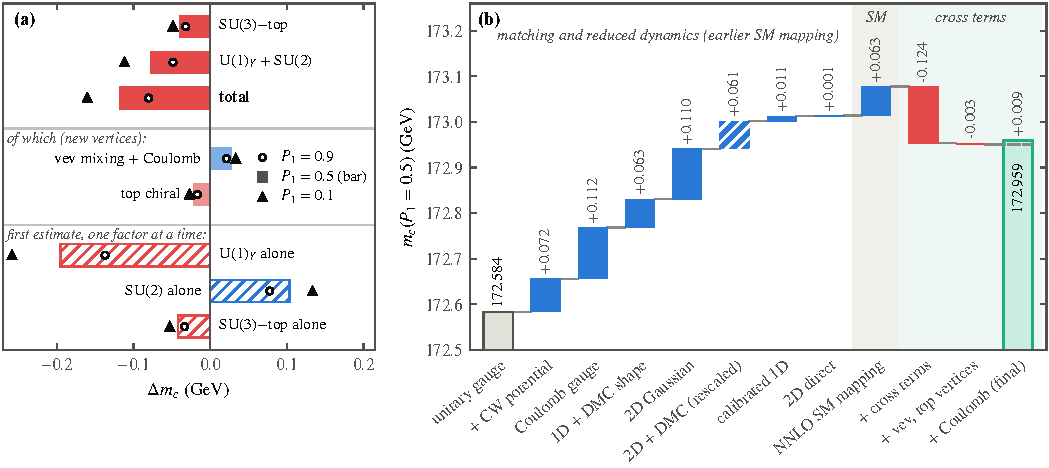
\includegraphics[width=\textwidth]{prd_cross_terms}
\caption{Zero-mode cross terms and the refinement of the critical mass.
(a)~Shift of $m_c$ by the one-loop cross terms (bars: $\Pone=0.5$; circles: $0.9$; triangles: $0.1$), split by gauge factor in the final model, with the new-vertex groups contained in the total, which is $-0.118\GeV$ at $\Pone=1/2$. %
Hatched: first estimate at fixed couplings, one gauge factor at a time (not additive).
(b)~$m_c(\Pone=1/2)$ along the model refinements of Table~\ref{tab:rb-convergence}, ending at $172.96\GeV$; the early steps add distinct physics rather than forming a convergence sequence, and the last two steps add the vev-mixing and top chiral vertices and then the Coulomb mismatch of the final model.} %
\label{fig:rb-cross}
\end{figure}

\section{Higgs zero mode IV: survival along the turn}\label{rep:h-survival}

Along the turn the couplings run and the conformal time is finite, so the zero mode decays with a time-dependent hazard.
We show that the hazard gives the survival probability of the resonant component of a time-symmetric real state, exactly in the adiabatic limit and to $0.2\%$ in a real-time evolution of the final model, that the minimal-variance rule of assumption (A8) fixes the weight of that component to $w_0=0.980$--$0.995$, and that the criterion barely depends on this weight. %
For a Higgs curvature coupling $\xiH<1/6$ the late turn adds an inverted oscillator, which we follow with an exact lens transformation and a quantum--classical switch; this machinery fixes the threshold $\xic$ of Sec.~\ref{rep:h-universality}.
Finally we show that the joint survival of both branches of the turning point has no probability in the decoherent-histories sense, so we quote single-branch probabilities throughout.
These are the measure statements of assumption (A4) of Sec.~\ref{rep:setup}.

\subsection{The turn as seen by the zero mode}
\label{sec:rb-turn}

The turning solution of Sec.~\ref{rep:turning} is $a^2=\cosh2\tau$ with $\tau\equiv ht$, so the edge of the torus grows as $L(\tau)=\Lb(\cosh2\tau)^{1/2}$.
Two consequences follow for the zero-mode problem, which lives in units of $1/L$.
First, the zero mode sees the Standard Model couplings at
\begin{equation}
\mu(\tau)=\frac{\mub}{(\cosh2\tau)^{1/2}},
\label{eq:rb-mutau}
\end{equation}
which we call the nodes of the hazard.
Second, its natural clock is the conformal time measured in units of $\Lb$.
With $d\eta=dt/(a\Lb)$,
\begin{equation}
d\eta=\frac{d\tau}{h\Lb(\cosh2\tau)^{1/2}},\qquad
\eta_\infty=\frac{1}{h\Lb}\int_0^\infty\frac{d\tau}{(\cosh2\tau)^{1/2}}=\frac{\Gamma(\frac14)^2}{4\sqrt{2\pi}\,h\Lb}=\frac{1.31103}{h\Lb}, %
\label{eq:rb-etainf}
\end{equation}
where we used $\int_0^\infty\cosh^{-\nu}x\,dx=2^{\nu-2}\Gamma(\nu/2)^2/\Gamma(\nu)$ at $\nu=\frac12$.
With $h\Lb=0.00437243$ the conformal duration of one branch is $\eta_\infty=299.84$, and the nodes $\tau\le5$ cover all but $\sqrt2\,e^{-5}/1.31103=0.7\%$ of it. %
This value of $h\Lb$ differs by $1\%$ from the instantaneous-reheating normalization of Sec.~\ref{rep:turning}, which would shift $m_c$ by at most $0.002\GeV$. %
The turning solution also has constant curvature: from $\dot a/a=h\tanh2\tau$ and $\dot a^2+a\ddot a=2h^2\cosh2\tau$,
\begin{equation}
R=6\Bigl(\frac{\ddot a}{a}+\frac{\dot a^2}{a^2}\Bigr)=12h^2,\qquad \frac{a''}{a}=2h^2a^2\Lb^2=2(hL)^2,
\label{eq:rb-R}
\end{equation}
where a prime denotes $d/d\eta$; both relations are used for the curvature coupling in Sec.~\ref{sec:rb-late}.

\subsection{Hazard and single-branch survival probability}
\label{sec:rb-hazard}

At each of eleven nodes $\tau=0,0.5,\ldots,5$ we recompute the gauge profiles, the matching $\Delta V_{\rm MC}$, and the cross terms with the Standard Model couplings at $\mu(\tau)$, and we solve directly for the two-dimensional resonance (Sec.~\ref{sec:rb-nodes}).
The width $\Gamma(m_t,\tau)$ is a rate in conformal time, so the hazard and the single-branch survival probability are
\begin{equation}
I(m_t)=\int_0^5\frac{\Gamma(m_t,\tau)\,d\tau}{h\Lb(\cosh2\tau)^{1/2}},\qquad \Pone=e^{-I}.
\label{eq:rb-hazard}
\end{equation}
We interpolate $\ln\Gamma$ between the eleven nodes with a cubic spline, integrate with Simpson's rule on $20\,001$ points, and find $m_c$ as the root of a cubic spline of $\ln I$ in $m_t$ on the grid $172.0$--$173.8\GeV$. %
Twenty-nine nodes instead of eleven change $m_c$ by $7\times10^{-5}\GeV$. %
The hazard-equivalent threshold is the Standard Model quartic at $\mub$ evaluated at the critical mass, $\lamc(\mub)\equiv\lambda_{\rm SM}(\mub;m_c)=-0.0091$, $-0.0121$, and $-0.0152$ for $\Pone=0.9$, $0.5$, and $0.1$. %

If instead the width at $\tau=0$ were held for the whole branch, the static condition $\Gamma=-\ln P/\eta_\infty$, that is $\Gamma_c=3.514\times10^{-4}$ and $2.312\times10^{-3}$ for $P=0.9$ and $0.5$, would give the static thresholds $-0.00880$, $-0.01174$, and $-0.01472$ in the earlier model, which we quote only for comparison. %
Because $|\lambda(\mu)|$ and hence $\Gamma$ decrease along the turn, the static thresholds lie $0.0003$ to $0.0004$ above the hazard-equivalent ones of the same model. %
For the same reason the integrand of Eq.~(\ref{eq:rb-hazard}) is largest early in the turn [Fig.~\ref{fig:rb-hazard}(a)].
At $\alpha_s=0.1180$ we find $\Pone=0.9976$, $0.9850$, $0.9424$, $0.8426$, $0.6721$, $0.4549$, $0.2508$, $0.1093$, $0.0372$, and $0.0099$ for $m_t=172.0$ to $173.8\GeV$ in steps of $0.2\GeV$. %
Near the critical masses $d\ln I/dm_t=5.27$, $3.22$, and $2.12\GeV^{-1}$ at $\Pone=0.9$, $0.5$, and $0.1$, the slopes that convert width ratios into shifts of $m_c$ throughout Secs.~\ref{rep:h-reduced}--\ref{rep:h-budget}. %

\subsection{Real initial states and the survival measure}
\label{sec:rb-measure}

The width is a property of the resonance; the survival probability of a given state also depends on how much of it is resonant.
At $\tau=0$ the state of the zero mode is real and time-reflection invariant, $\psi(-\eta)=\psi(\eta)^*$.
We decompose it with the c-product $(\varphi,\psi)=\int\varphi\,\psi$ (no complex conjugation), under which the resonance $\varphi_{\rm res}$ is normalizable and orthogonal to the other eigenfunctions of the complex-symmetric Hamiltonian with an absorbing potential:
\begin{equation}
\psi_0=(\varphi_{\rm res},\psi_0)\,\varphi_{\rm res}+\psi_\perp,\qquad w_0\equiv|(\varphi_{\rm res},\psi_0)|^2 .
\label{eq:rb-decomp}
\end{equation}
The resonant part follows the instantaneous resonance adiabatically and loses norm at the hazard rate, while the non-resonant part $\psi_\perp$ lies above the barrier and leaves the well within $\Delta\eta\lesssim40$, about $\Delta\tau\lesssim0.2$. %
The in-well probability at the end of the branch is therefore
\begin{equation}
P_\infty=w_0\,P_{\rm haz,\infty}\,(1+\delta),\qquad P_{\rm haz}=\exp\Bigl(-\int\Gamma\,d\eta\Bigr),
\label{eq:rb-w0}
\end{equation}
where $\delta$ comes only from the definition of the in-well probability (cutting at the barrier top).

We verified Eq.~(\ref{eq:rb-w0}) by evolving real states with the time-dependent Schr\"odinger equation in the conformal frame.
The spatial discretization is a five-point fourth-order Laplacian with $dr=0.01$ up to $r=16$ and odd continuation at the origin, which gives the regular behavior $r^{s_0}$; time stepping is Crank--Nicolson with $d\eta=0.025$; beyond $r_c=10$, about twice the exit point, the potential is smoothly flattened and a quadratic absorbing potential removes the outgoing flux. %
The resonance is continued from node to node as an eigenvalue of the complex-symmetric Hamiltonian with the absorbing potential; its width agrees with the Siegert width to $0.2\%$ and its energy to $1.5\times10^{-6}$ at all nodes. %
In a one-dimensional model without cross terms, with the earlier mapping, the resonant projection decays at the hazard rate to $1.3\times10^{-4}$ for $\tau\le5$, and $|\delta|\le0.3\%$. %
Gamow-like states, the real part of the c-normalized resonance cut at the outer turning point or the ground state with a Dirichlet wall at $1.0$ or $1.2$ times the exit radius, have $w_0=0.9997$--$1.0019$ and $P_\infty/P_{\rm haz,\infty}-1\in[-0.34\%,+0.01\%]$. %
For every other real state we tried, the remainder decays at the hazard rate after the non-resonant part has left, so that $P_\infty=w_0P_{\rm haz,\infty}$.
An independent reimplementation reproduces $P_\infty=w_0P_{\rm haz,\infty}$ with projection deviations below $10^{-3}$; for the walled ground state at $1.2$ times the exit radius it finds $w_0=1.0019$ and $P_{\rm haz,\infty}=0.47706$ against $0.4770$ (Sec.~\ref{rep:v-blind}). %
In the final two-dimensional model the absorbing-potential pole at $\tau=0$ agrees with the Siegert root to $0.08\%$ in $\Gamma$, the Gamow-like state has $w_0=1.0000$--$1.0013$, and with $\xiH=1/6$ the real-time survival probability equals the hazard $\Pone$ to $0.22\%$. %
The hazard is therefore the survival measure conditional on the zero mode being in the metastable sector, and $w_0$ is a separate preparation factor.
We use only Lorentzian widths: a Euclidean preparation is ill defined for a negative quartic, and $w_0$ parametrizes the preparation instead.

\subsection{Preparation weight}
\label{sec:rb-w0}

For $P=w_0\Pone$ the critical masses depend on $w_0$ as in Table~\ref{tab:rb-w0}; for $w_0<0.9$ the level $P=0.9$ is never reached. %
The criterion barely depends on the preparation: even $w_0=0.9$ or $0.8$ would lower the critical mass for probability $1/2$ by only $0.050$ or $0.114\GeV$. %

\begin{table}[t]
\centering
\caption{Shift of the critical top mass (GeV) for a survival probability $P=w_0\Pone$, relative to $w_0=1$, at $\alpha_s(M_Z)=0.1180$, computed with the cross terms before their final one-loop corrections; for the minimal-variance weights the final model gives the same shifts to $0.001\GeV$.} %
\label{tab:rb-w0}
\begin{tabular}{cccc}
\toprule
$w_0$ & $P=0.9$ & $P=0.5$ & $P=0.1$ \\
\midrule
$0.99$ & $-0.019$ & $-0.005$ & $-0.002$ \\ %
$0.95$ & $-0.118$ & $-0.024$ & $-0.011$ \\ %
$0.9$ & --- & $-0.050$ & $-0.022$ \\ %
$0.8$ & --- & $-0.114$ & $-0.047$ \\ %
$0.55$ & --- & $-0.475$ & $-0.134$ \\ %
\bottomrule
\end{tabular}
\end{table}

To fix $w_0$ we apply to the Higgs zero mode the rule that selects the shape state at the turning point (assumption (A8) and Sec.~\ref{rep:quantum-shape}): among real, time-symmetric central Gaussians, take the one with the smallest instantaneous energy variance.
We use the two-dimensional model at $\tau=0$,
\begin{equation}
H=-\tfrac12\partial_r^2+U_1(r)+T_s+\tfrac12\Omega^2(r)s^2+V_L(r,s),
\label{eq:rb-H-B3}
\end{equation}
with $U_1$ the $r$-dependent potential of Eq.~(\ref{eq:rb-U1}) plus the radial cross terms of Sec.~\ref{rep:h-cross}, $T_s$ the kinetic term of $\bm w$, and $V_L$ the light-fermion twist energy of Eq.~(\ref{eq:rb-VL}), discretized with $h=0.01$ in $r$ and the $s$ basis of the hazard code. %
The potential has its minimum at $\Phi=0$, $\bm w=0$; the term $3/(8r^2)$ comes from the radial reduction in four dimensions and is not part of the potential.
Under SO(4)$\times$SO(3) there is no invariant bilinear form between $\Phi$ and $\bm w$, so the most general real central Gaussian is
\begin{equation}
\psi_{\rm G}\propto\exp\Bigl(-\frac{r^2}{2\sigma_r^2}-\frac{|\bm w|^2}{2\sigma_s^2}\Bigr),\qquad r=|\bm\phi|,
\label{eq:rb-B3}
\end{equation}
with two widths.
These states behave as $u\propto r^{3/2}$, lie in the domain of $H$, and have finite variance; their tail at the barrier, $r\approx5$, is about $e^{-14}$, so the runaway region does not contribute. %
The variance $\langle H^2\rangle-\langle H\rangle^2$ has a unique minimum at $\sigma_r=1.33$--$1.36$ and $\sigma_s\approx1.36$, within $1$--$3\%$ of the energy-minimizing Gaussian. %

We compute $w_0=|\langle\varphi_{\rm res}|\psi_{\rm G}\rangle|^2$ with $\varphi_{\rm res}$ either the walled quasi-bound state, with walls at $1.1$, $1.2$, and $1.4$ times the outer turning point, or the c-normalized resonance from the absorbing potential. %
The walled energies agree with the real parts of the Siegert roots to between $6\times10^{-6}$ and $8\times10^{-4}$. %
We find $w_0=0.995$, $0.991$, $0.985$--$0.990$, and $0.980$--$0.988$ at $m_t=172.2$, $172.6$, $173.0$, and $173.4\GeV$, and at $172.6\GeV$ the absorbing-potential projection gives $0.9921$--$0.9923$. %
The weight does depend on the widths, since scaling $\sigma_r$ by $0.85$ or $1.15$ gives $0.928$ or $0.972$; it is the rule, not the Gaussian form alone, that fixes $w_0\approx0.99$. %
Over all real states the minimal variance tends to zero and selects the quasi-stationary state itself, $w_0\to1$; the derived range is $w_0\in[0.980,1]$. %
A blind reimplementation in the one-dimensional reduction gives $w_0=0.991$--$0.996$ (Sec.~\ref{rep:v-blind}). %

With $w_0(m_t)$ from the rule the critical masses of the final model are $172.486$, $172.953$, and $173.414\GeV$ at $P=0.9$, $0.5$, and $0.1$, a shift between $-0.0160$ and $-0.0129\GeV$, between $-0.0065$ and $-0.0043\GeV$, and between $-0.0041$ and $-0.0025\GeV$ for the different projections. %
The error budget carries the largest shifts, $-0.016$, $-0.006$, and $-0.004\GeV$, as one-sided errors (Sec.~\ref{rep:h-budget}). %
The weight uses the $\tau=0$ Hamiltonian with the cross terms of the charged-component approximation; the final one-loop corrections change the adiabatic potential by only $-0.001$ to $+0.004/L$ at $r=1$--$5$, which leaves $w_0$ unchanged at the quoted precision. %
A Gaussian in the radial variable that is centred at the bottom of the well and cut off at the origin gives $w_0=0.71$--$0.76$ and $0.85$ for one and two well widths, but it is not in the domain of $H$: $\langle3/(8r^2)\rangle$ diverges, and on the grid its energy and energy spread are about $19$ and $317$. %
The minimal-variance rule excludes such constructions.

\subsection{The late turn: conformal frame, lens transformation, and quantum--classical switch}
\label{sec:rb-late}

With $\xiH=1/6$ the curvature term of the zero-mode equation vanishes, and the hazard to $\tau=5$ gives the survival probability.
For $\xiH<1/6$ the late turn matters, and we derive here the equations that we evolve.

\paragraph{Conformal frame.}
For a scalar with action $\int d^4x\sqrt{-g}\,[-\frac12(\partial\phi)^2-\frac12\xiH R\phi^2-V(\phi)]$ in the metric $a^2(\eta)(-d\eta^2+d\bm x^2)$, the rescaled field $\chi=a\phi$ has, after an integration by parts,
\begin{equation}
\mathcal L_\chi=\tfrac12\chi'^2-\tfrac12(\nabla\chi)^2+\tfrac12(1-6\xiH)\frac{a''}{a}\chi^2-a^4V(\chi/a),
\label{eq:rb-Lchi}
\end{equation}
because $\sqrt{-g}R=6a\,a''$.
The quartic is conformal, $a^4V(\chi/a)=\lambda\chi^4/4$, and the zero-mode potential and the matching are evaluated with the couplings at $1/L$.
With $a''/a=2(hL)^2$ from Eq.~(\ref{eq:rb-R}), the zero mode obeys
\begin{equation}
i\partial_\eta\psi=\Bigl[-\tfrac12\partial_r^2+U_{\rm nc}(r;\tau)-(1-6\xiH)(hL)^2r^2\Bigr]\psi,
\label{eq:rb-conformal}
\end{equation}
where $U_{\rm nc}$ is the reduced potential without the curvature term and $hL=h\Lb(\cosh2\tau)^{1/2}$.
For $\xiH<1/6$ the last term is an inverted harmonic potential that grows like $\cosh2\tau$ and dominates at $\tau\gtrsim4$.

\paragraph{Lens transformation.}
For a Hamiltonian $-\frac12\partial_r^2+\frac12\omega^2(\eta)r^2+V(r,\eta)$ and any positive scale $s(\eta)$, the substitution
\begin{equation}
\psi(r,\eta)=s^{-1/2}\exp\Bigl(\frac{is'}{2s}r^2\Bigr)\,\Phi\Bigl(\frac rs,T\Bigr),\qquad \frac{dT}{d\eta}=\frac1{s^2},
\label{eq:rb-lens-general}
\end{equation}
gives
\begin{equation}
i\partial_T\Phi=\Bigl[-\tfrac12\partial_y^2+\tfrac12s^3\bigl(s''+\omega^2s\bigr)y^2+s^2V(sy,\eta)\Bigr]\Phi,\qquad y=\frac rs,
\label{eq:rb-lens-ermakov}
\end{equation}
as follows by direct differentiation: the phase removes the dilation generated by the time-dependent rescaling and leaves the $s''$ term.
We choose $s=hL$, for which $s''/s=L''/L=2(hL)^2$ by Eq.~(\ref{eq:rb-R}), and $\omega^2=-2(1-6\xiH)(hL)^2$ from Eq.~(\ref{eq:rb-conformal}).
Then $s''+\omega^2s=12\xiH(hL)^3$: the conformal part of the inverted oscillator is cancelled exactly, and only the curvature coupling remains.
Measuring time in $\tau$, $d\tau=hL\,d\eta=s^3dT$, gives
\begin{align}
\Phi(y)&=(hL)^{1/2}e^{-i(L'/L)r^2/2}\,\psi(hLy),\qquad y=\frac{r}{hL},\qquad \frac{L'}{L}=hL\tanh2\tau,\nonumber\\
i\partial_\tau\Phi&=\Bigl[-\frac{\partial_y^2}{2M}+\frac{U_{\rm nc}(hLy;\tau)}{hL}+6\xiH My^2\Bigr]\Phi,\qquad M=(hL)^3 .
\label{eq:rb-lens}
\end{align}
The map is exact and takes the problem to the physical field $y=\phi/h$.
It is the quantized zero mode of the Lagrangian $L^3[\frac12\dot\phi^2-6\xiH h^2\phi^2-U_{\rm nc}(L\phi)/L^4]$: the conformal term becomes the curvature mass squared $\xiH R=12\xiH h^2$, and the growing effective mass $M$ makes the late dynamics classical.
Mapping at $\tau=4.0$ or $4.5$ gives norms and survival probabilities that agree to $5\times10^{-5}$. %
In the physical frame we use $dy=0.003$ up to $y=64$ and an absorber that starts at $\max(1.5\,y_{\rm top},10)$, with $y_{\rm top}$ the instantaneous barrier top; all trajectories absorbed there run away classically. %
A sharp absorber reflects about $0.5\%$ at $\tau\approx4$--$4.5$, and a smooth one removes this. %

\paragraph{Quantum--classical switch.}
At $\tau_{\rm sw}$ we compute Wigner weights averaged over momentum cells on a $320\times200$ grid, checked on $480\times300$, keep the negative weights, and follow each phase-space cell as a classical trajectory in cosmic time,
\begin{equation}
y''+3\tanh(2\tau)\,y'+12\xiH\,y+\frac{U_{\rm nc}'(hL\,y;\tau)}{(hL)^3}=0,
\label{eq:rb-classical}
\end{equation}
up to $\tau=60$, where a prime now denotes $d/d\tau$ and $3\tanh2\tau=3H/h$ is the Hubble friction. %
A trajectory runs away when $y>\max(3y_b,30)$ and is bounded when $y<0.3$, or when $y<y_b$ and its energy is below $0.9$ of the barrier at $\tau>\max(\tau_{\rm sw}+2,7.5)$; Hubble friction lowers the energy monotonically, so the verdict cannot change later. %
The survival probability is the total bounded weight, and the flux absorbed in the quantum stage counts as runaway.
The full non-quartic force is kept in the classical stage, because at the barrier the force of the gauge zero modes and of the finite-volume matching is $1.66$, $0.33$, and $0.11$ times the curvature force at $\tau=5$ for $\xiH=0.04$, $0.1$, and $1/6$, and still $0.024$, $0.003$, and $0.002$ times it at $\tau=6$. %

The switch must be late enough.
At $\tau_{\rm sw}=5$ the effective mass is only $M=0.097$, and $\xic$ moves by up to $0.007$; for $\tau_{\rm sw}\ge5.5$ ($M\ge0.43$) the results are stable, and a run without switch, carried to $\tau=7$ ($M=39$), agrees with $\tau_{\rm sw}=6$ to $10^{-4}$. %
For $\tau_{\rm sw}$ between $5.5$ and $6.5$ the survival probability changes by at most $2\times10^{-4}$ when $\lambda$ is frozen at $\mu=1/L$, and by up to $3\times10^{-3}$ at $\xiH=0.04$ when $\lambda$ runs with the field; in the final model this moves $\xic$ by at most $0.0005$. %
Momentum-cell Wigner sampling and a Madelung (hydrodynamic) version give the same $\xic$ to $10^{-4}$. %
Tunneling after $\tau_{\rm sw}$, which the truncated Wigner treatment omits, is bounded by this stability.
During the classical stage the scale of $\lambda$ is ambiguous; we use two prescriptions, $\lambda$ at $\mu=(\phi^2+H^2+\mu(\tau)^2)^{1/2}$, which follows the field, and $\lambda$ at $1/L$, frozen for $\tau>7$ because the running would take $\mu$ below the electroweak scale by $\tau=60$, and we quote the midpoint and half the difference.

\paragraph{Calibrated one-dimensional evolution and the two-dimensional check.}
The real-time chain runs on a one-dimensional effective potential.
At each of $29$ nodes, $\tau=0$ to $7$ in steps of $0.25$, we reduce the final two-dimensional Hamiltonian adiabatically, $U_{\rm BO}=U_1+\varepsilon_0$, where $\varepsilon_0(r)$ is the exact ground energy of the $\bm w$ channel including the light-fermion twist, and add a bump $A(\tau)\exp[-((r-2.30)/0.35)^2]$. %
We calibrate $A$ at the eleven hazard nodes so that the one-dimensional Siegert width equals the two-dimensional width, and hold it beyond $\tau=5$; the calibration converges to $|\Delta\ln\Gamma|\le1.5\times10^{-6}$ with $A=0.0130\pm0.0004$. %
Without the bump the widths are $1.0$--$1.8\%$ too low; the cross terms stiffen the $\bm w$ direction and make it nearly adiabatic, so the correction is small. %
A two-dimensional real-time evolution of the same model in $(r,s)$ tests the reduction.
It uses Strang splitting, with the stiff one-dimensional part, which includes $3/(8r^2)$, the absorber, and the flattening, inside a Crank--Nicolson step and the $\bm w$ coupling $\frac12\Omega_{\rm eff}^2s^2+V_L-\varepsilon_0$ in half steps; at $\tau_{\rm sw}$ it projects onto the instantaneous $\bm w$ channels and samples each channel separately.
Excited channels carry $0.10$--$0.63\%$ of the probability at $\tau_{\rm sw}=6$, and treating $\bm w$ classically in the truncated Wigner approximation changes $P_{\rm surv}$ by at most $10^{-6}$ for $\xiH\ge0.02$. %
For $\xiH\ge0.02$ the two-dimensional and one-dimensional survival probabilities agree to $2\times10^{-4}$ at twenty points, and $\xic$ agrees to $1.4\times10^{-4}$, five to thirty times below the prescription bands. %
Halving the time steps changes $P_{\rm surv}$ by $1.4\times10^{-4}$, and a larger $s$ basis by $10^{-6}$. %

\paragraph{The case $\xiH=0$.}
For $\xiH=0$ the zero mode runs away.
At $m_t=172.6\GeV$ the fraction that is not yet classified as runaway after $30$, $60$, and $120$ $e$-folds is $0.345$, $0.147$, and $0.052$ (for $\lambda$ at $1/L$), almost all of it on undecided trajectories, and it tends to zero as the number of $e$-folds grows. %
For a homogeneous field in de~Sitter space with $R=12H^2$ the curvature barrier is $\Delta V=36\xiH^2H^4/|\lambda|$, and the Hawking--Moss exponent is $B=8\pi^2\Delta V/(3H^4)=96\pi^2\xiH^2/|\lambda|$~\cite{Hawking:1981fz}. %
At $\xiH=\xic$ the zero mode's own quantum width at $\tau=6$ is $11$ to $60$ times the de~Sitter kick $H/2\pi$ per $e$-fold, so stochastic kicks are a small perturbation of a spread that the Wigner evolution already contains. %
The evolution of the zero mode together with the non-zero modes after the lowest non-zero modes leave the Hubble radius, at $\tau\approx7.6$, is not simulated; it can only lower $P_{\rm surv}$, by an estimated few percent of the probability near the barrier at $\xiH\approx\xic$. %
Inside the curvature barrier, for $y_b/\sqrt3<y<y_b$ with $y_b$ the top of the barrier, the potential is concave, so superhorizon non-zero modes grow there. %
They grow only briefly, before the zero mode is pulled back, so the instability acts only on the part of the probability that reaches the barrier; since it can only lower $P_{\rm surv}$, it can only raise $\xic$. %

\begin{figure}[t]
\centering
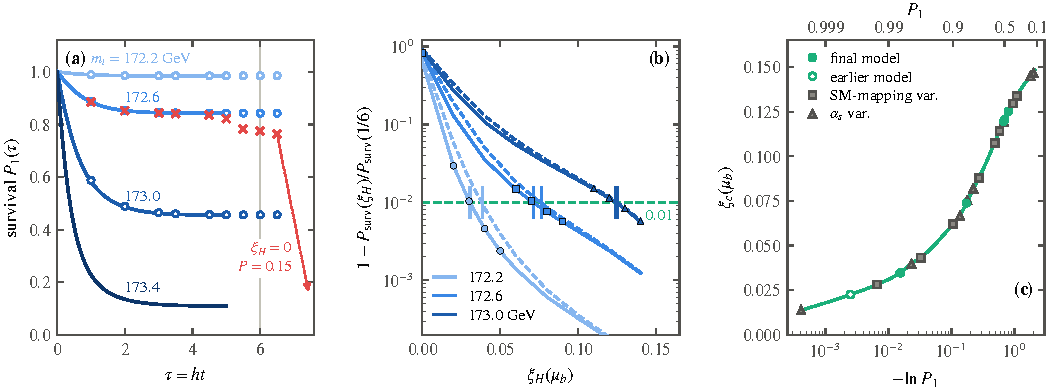
\includegraphics[width=\textwidth]{prd_hazard_realtime}
\caption{Survival along the turning solution and the role of $\xiH$.
(a)~Hazard survival $\Pone(\tau)$ for $m_t=172.2$--$173.4\GeV$ with the norm of the real-time evolution at $\xiH=1/6$ (circles) and $\xiH=0$ (crosses; arrow: final value after the classical stage, which starts at $\tau=6$). %
(b)~Relative loss $1-P_{\rm surv}(\xiH)/P_{\rm surv}(1/6)$ from one-dimensional (lines; solid and dashed: two prescriptions for $\lambda$) and two-dimensional (markers) real-time evolution; the $1\%$ line defines $\xic$ (ticks).
(c)~$\xic$ depends on $m_t$, $\alpha_s$, and the Standard Model mapping only through $\Pone$, tested for $0.45\lesssim\Pone\lesssim0.998$ (final model; earlier model and its variants).} %
\label{fig:rb-hazard}
\end{figure}

\subsection{Two branches}
\label{sec:rb-branches}

A turning point is time symmetric, and in the reading of assumption (A4) both halves $\tau<0$ and $\tau>0$ are expanding branches (Sec.~\ref{rep:gate}).
By time-reflection symmetry $\Pone$ is the same for both.
We show that their joint survival is not a probability in the decoherent-histories sense~\cite{Gell-Mann:1991kdm,Goldstein:1994cp}.

\paragraph{Setup.}
With $\xiH=1/6$ the zero-mode Hamiltonian $H(\eta)$ is real and even in $\eta$.
With complex conjugation $K$ the propagator obeys $KU(\eta_2,\eta_1)K=U(-\eta_2,-\eta_1)$, since both sides solve the same equation with the same initial value.
Let $P$ project onto $r<r_{\rm top}$ and define the Heisenberg projectors at the turning point
\begin{equation}
E_+=U(T,0)^\dagger PU(T,0),\qquad E_-=KE_+K .
\label{eq:rb-Epm}
\end{equation}
For a real $\psi_0$ the single-branch probabilities are equal, $\Pone=\langle\psi_0|E_+|\psi_0\rangle=\langle\psi_0|E_-|\psi_0\rangle$.
A probability for the joint event needs a decoherent set of histories~\cite{Gell-Mann:1991kdm}.
The two-time set $C_{ab}=P_b(T)P_a(-T)$, with $a,b\in\{{\rm in},{\rm out}\}$, has decoherence functional $D(h,h')=\langle C_{h'}\psi_0|C_h\psi_0\rangle$.
With $A=P\psi(T)$, time reflection gives $P\psi(-T)=A^*$.
Define $X=PU(T,-T)A^*$ and $Y=A-X$.
Then
\begin{equation}
D({\rm in},{\rm in})=\|X\|^2,\qquad D({\rm out},{\rm in})=\|Y\|^2,\qquad
D_{\rm off}=\langle Y|X\rangle=\langle A|X\rangle-\|X\|^2,
\label{eq:rb-decoh}
\end{equation}
and the linear value is $K_{\rm lin}=\langle E_+\psi_0|E_-\psi_0\rangle=\langle A|X\rangle$.
Only two forward evolutions from states localized in the well are needed, and the absorber is exact for them because outgoing flux never returns.
The interference ratio is $\varepsilon=|D_{\rm off}|/[D({\rm in},{\rm in})D({\rm out},{\rm in})]^{1/2}$.

\paragraph{Three statements.}
(i)~For a real $\psi_0$ the reversed set $P_a(-T)P_b(T)$ has the complex-conjugate functional with the branch labels exchanged, so the order of times plays no role.
(ii)~If the in-well part is the adiabatic resonance after the initial transient, $P\psi(T)=c\,P_h(T)^{1/2}e^{-i\theta}\varphi_T$ with $|c|^2=w_0$, and the resonance decays from $-T$ to $T$ with $P_h(T)^2$, then $X\parallel A$ and $\varepsilon=1$: the set has maximal interference.
In this limit $D({\rm in},{\rm in})=\Pone^3/w_0^2$ and ${\rm Re}\,K_{\rm lin}=(\Pone^2/w_0)\cos2\alpha$ with $\alpha=\arg c$.
For $w_0=1$ the diagonal element $\Pone^3$ falls below the Fr\'echet bound $2\Pone-1$ when $\Pone>(\sqrt5-1)/2=0.618$, so it cannot be a probability. %
Physically, the decayed component of the $-$ branch at $-T$ is, read forward, the incoming flux that refills the resonance at the turning point; both outcomes of the $-$ branch feed the same surviving state of the $+$ branch, which keeps no record of them.
(iii)~A joint distribution with marginals $E_-$ and $E_+$ for all states exists only if $[E_+,E_-]=0$: from $0\le M_{a,{\rm in}}\le E_+$ it follows that $M_{a,{\rm in}}=E_+M_{a,{\rm in}}E_+$, and similarly for out, so that $E_-^a$ commutes with $E_+$.
In the resonance limit $\|[E_+,E_-]\psi_0\|^2\simeq2\Pone^3(1-\Pone)$, which is $0.19$ at $\Pone=0.84$. %
Quantum mechanics then fixes only the Fr\'echet bounds
\begin{equation}
\max(0,2\Pone-1)\le P_2\le\Pone
\label{eq:rb-frechet}
\end{equation}
on any joint probability $P_2$ with marginals $\Pone$.
Among bilinear assignments $\frac12\{E_+,E_-\}+c\,i[E_+,E_-]$ that reduce to the joint spectral measure for commuting projectors, symmetry under exchange of the branches fixes $c=0$, which leaves the linear (Margenau--Hill) value $P_2^{\rm lin}={\rm Re}\langle\psi_0|E_+E_-|\psi_0\rangle$ of Ref.~\cite{Goldstein:1994cp}.

\paragraph{Numerics.}
For three top masses, six real initial states, and four numerical variants in the one-dimensional model, $\varepsilon=0.9948$--$0.99997$ for $\tau_T\ge1$, the ratio $D({\rm in},{\rm in})\,w_0^2/\Pone^3$ is $1$ to $10^{-4}$, ${\rm Re}\,K_{\rm lin}\,w_0/\Pone^2=0.99993$--$1.000002$, and $|{\rm Im}\,K_{\rm lin}/{\rm Re}\,K_{\rm lin}|\le0.012$. %
A propagation by dense eigendecomposition of the frozen $\tau=0$ Hamiltonian, independent of the Crank--Nicolson stepping, gives $\varepsilon=0.99983$--$0.999996$ and the same linear value to $2\times10^{-5}$. %
The four linear cells are non-negative and lie inside the Fr\'echet band of Eq.~(\ref{eq:rb-frechet}).
If the linear value $P_2=\Pone^2/w_0$ is adopted with $w_0=1$, $m_c(P_2=p)=m_c(\Pone=\sqrt p)$; in the final model this gives $172.380$, $172.764$, and $173.131\GeV$ for $P_2=0.9$, $0.5$, and $0.1$, which is $0.122$, $0.195$, and $0.288\GeV$ below the single-branch values. %
The Fr\'echet band alone allows shifts between $-0.126$ and $0\GeV$ for $P_2=0.9$ and between $-0.241$ and $0\GeV$ for $P_2=0.5$. %
These statements, derived in the one-dimensional zero-mode model, carry over to the two-dimensional model, which has the same time-reflection symmetry and a single resonance.

The shape sector differs in this respect: there the branch that does not cross the turn never failed in any run, so the two-branch survival of the shape equals the single-branch survival of the crossing branch to $4\times10^{-4}$ (Sec.~\ref{rep:quantum-shape}), whereas for the Higgs zero mode both branches decay and their joint survival has no probability. %
We quote single-branch probabilities throughout.

\section{Standard Model mapping and the top-quark criterion}\label{rep:h-smmap}

The Standard Model enters the Higgs calculation through the couplings $(\lambda,g_2,g_Y,g_3,y_t)$ at the nodes $\mu(\tau)$ of Eq.~(\ref{eq:rb-mutau}).
We map the threshold of Secs.~\ref{rep:h-reduced}--\ref{rep:h-survival} to the top-quark mass with three-loop Standard Model running and next-to-next-to-leading-order (NNLO) matching, computed with our own code (assumption (A2) of Sec.~\ref{rep:setup}).
With $m_t$ the top-quark pole mass and $\mtbar\equiv\mtbar(\mtbar)$ the $\MSbar$ mass of assumption (A7), the result is
\begin{equation}
P_1>\tfrac12 \;\Longleftrightarrow\; m_t<172.96~\mathrm{GeV}
\quad\bigl[\,\bar m_t<163.16~\mathrm{GeV}\,\bigr], %
\label{eq:rb-criterion}
\end{equation}
for $\alpha_s(M_Z)=0.1180$; the Standard Model theory error is $\pm0.10\GeV$ for $m_t$ and $\pm0.07\GeV$ for $\mtbar$, and $\alpha_s\pm0.0009$ moves the bound by $\pm0.35\GeV$ ($\pm0.25\GeV$ for $\mtbar$). %
The levels $\Pone=0.9$ and $0.1$ give $m_t=172.50$ and $173.42\GeV$ ($\mtbar=162.73$ and $163.60\GeV$). %
The criterion lies $m_c-m_0=\mcMinusMzero\GeV$ above the line $\lambda(\mub)=0$, at $m_0=171.09\GeV$, which in turn lies $0.10\GeV$ above the absolute-stability line of the same mapping, $m_t=170.99\GeV$, computed for this report (Sec.~\ref{sec:rb-absstab}). %
We also show that the larger scale dependence of the tadpole-including organization of the fixed-order matching comes from same-sign two-loop logarithms in the $G_F$ scheme rather than from tadpoles.
We use $\MSbar$ couplings with $g_Y=g'=\sqrt{3/5}\,g_1^{\rm GUT}$ and $V=\lambda(|H|^2-v^2/2)^2$, and $\mub=\MPbar/722=3.3726\times10^{15}\GeV$. %

\subsection{Matching at the top-quark mass}
\label{sec:rb-sm-matching}

At $\mu_0=m_t$ we take the reference model of SMDR~1.3~\cite{Martin:2019lqd}, which uses the tadpole-free pure $\MSbar$ scheme with inputs $(G_F,\alpha,M_Z,M_h,m_t,\alpha_s)$, complete two-loop and leading three-loop threshold corrections, and four-loop QCD for the top mass.
We move it to the desired $(m_t,\alpha_s,M_h)$ with the linear slopes of Ref.~\cite{Buttazzo:2013uya}.
Across the reference models of several releases this shift reproduces $\lambda$, $y_t$, and $g_3$ at $m_t$ to $2.3\times10^{-5}$, $4.9\times10^{-6}$, and $3.8\times10^{-6}$, and the quartic at $\mub$ to $3.9\times10^{-5}$, which is $0.006\GeV$ in $m_t$. %
We also compiled SMDR and fitted the inputs directly.
At $\mu=m_t$ the compiled fit and the shifted reference model differ by at most $3.0\times10^{-6}$ in $\lambda$ and $7.4\times10^{-6}$ in $y_t$, and in the hazard the two give critical masses within $0.005\GeV$. %
A fit with all evaluation scales at their default values reproduces every $\MSbar$ parameter of the reference model to $8\times10^{-13}$. %

\subsection{Running to the bounce scale}
\label{sec:rb-sm-running}

The $\beta$ functions are generated automatically from the SMDR source: complete three-loop Standard Model running~\cite{Mihaila:2012fm,Bednyakov:2012rb,Bednyakov:2012en,Bednyakov:2013eba,Chetyrkin:2012rz,Chetyrkin:2013wya}, four-loop gauge couplings~\cite{Bednyakov:2015ooa,Zoller:2015tha,Davies:2019onf}, the leading four-loop QCD terms of $y_t$ and $\lambda$~\cite{Chetyrkin:1997dh,Vermaseren:1997fq,Martin:2015eia,Chetyrkin:2016ruf}, and five-loop QCD for $g_3$ and $y_t$~\cite{Baikov:2016tgj,Herzog:2017ohr,Baikov:2014qja}.
For orientation, the one-loop parts are
\begin{align}
16\pi^2\frac{dg_2}{d\ln\mu}&=-\frac{19}{6}g_2^3,\qquad 16\pi^2\frac{dg_Y}{d\ln\mu}=\frac{41}{6}g_Y^3,\qquad 16\pi^2\frac{dg_3}{d\ln\mu}=-7g_3^3,\nonumber\\
16\pi^2\frac{dy_t}{d\ln\mu}&=y_t\Bigl(\frac92y_t^2-8g_3^2-\frac94g_2^2-\frac{17}{12}g_Y^2\Bigr),
\label{eq:rb-beta1}
\end{align}
and $\beta_\lambda^{(1)}$ of Eq.~(\ref{eq:rb-betalam}); the term $-6y_t^4$ drives $\lambda$ negative at intermediate scales for the measured masses, and the decrease of $y_t$ (through $g_3$) makes $\lambda(\mu)$ turn up again at high scales~\cite{Degrassi:2012ry,Buttazzo:2013uya}; with our inputs the minimum lies near $5\times10^{17}\GeV$ (Sec.~\ref{sec:rb-absstab}). %
Light Yukawa couplings below $y_b$ are set to zero, which changes $\lambda$ by less than $10^{-6}$. %
A second implementation, copied by hand from the appendix of Ref.~\cite{Buttazzo:2013uya}, agrees term by term: to $4\times10^{-15}$ at one and two loops and for the three-loop gauge terms, and to $3.2\times10^{-6}$ ($y_t$) and $5.9\times10^{-5}$ ($\lambda$) at three loops, the rounding of the $\zeta_3$ coefficients in that appendix. %
Our running reproduces the published SMDR running up to $10^{19}\GeV$ with $|\Delta\lambda|\le9\times10^{-7}$, and an independent conversion of the same $\beta$ functions to Wolfram Language gives $\lambda(\mub)$ to $1.8\times10^{-14}$. %

\subsection{Pole and \texorpdfstring{$\MSbar$}{MS-bar} top masses}
\label{sec:rb-zm}

The pure-QCD part is our own code.
Pole and $\MSbar$ masses are related by
\begin{equation}
\frac{\mtbar(\mu)}{m_t}=z_m(\mu)=\sum_{k\ge0}a^kP_k\Bigl(\ln\frac{\mu^2}{m_t^2}\Bigr),\qquad a=\frac{\alpha_s^{(6)}(\mu)}{\pi},
\label{eq:rb-zm}
\end{equation}
where $P_k$ is a polynomial of degree $k$ whose constant term is $z_k$: $z_0=1$, $z_1=-4/3$, $z_2=-9.12549$, $z_3=-80.4057$, and $z_4=-859.96\pm21.5$~\cite{Marquard:2015qpa,Marquard:2016dcn}. %
The logarithmic coefficients follow from the renormalization group, $d\ln\mtbar/d\ln\mu=-\gamma_m(a)$ and $da/d\ln\mu=\beta(a)$, by requiring $m_t$ to be scale independent, and they reproduce the four published ones exactly.
We truncate the series at four loops ($k=4$), which defines the pole mass of assumption (A7), and decouple the top quark from $\alpha_s$ at four loops.
An independent symbolic derivation gives the same $z_2$, $z_3$, and logarithms, and $\alpha_s^{(6)}(172.4\GeV)=0.1077213$ agrees with a 25-digit numerical solution. %

\subsection{Couplings at \texorpdfstring{$\mub$}{mu-b}, linearization, and the criterion}
\label{sec:rb-sm-criterion}

For $(m_t,\alpha_s,M_h)=(172.60\GeV,0.1180,125.13\GeV)$ the couplings at $\mub$ are $\lambda=-0.0097741$, $y_t=0.4278267$, $g_2=0.527759$, $g_Y=0.442770$, and $g_3=0.535654$. %
Near the threshold the quartic at $\mub$ is nearly linear in the top mass,
\begin{equation}
\lambda(\mub;m_t)\simeq\frac{d\lambda(\mub)}{dm_t}\,(m_t-m_0),\qquad
\frac{d\lambda(\mub)}{dm_t}=-0.00652,\ -0.00657,\ -0.00661\GeV^{-1} %
\label{eq:rb-lin}
\end{equation}
at $m_t=172.2$, $172.6$, and $173.0\GeV$, where $m_0=171.09\GeV$ is the mass at which $\lambda(\mub)=0$. %
The hazard is computed at each $m_t$ with all couplings at the nodes, not from this linearization.
Since $\lamc(\mub)\equiv\lambda_{\rm SM}(\mub;m_c)$, dividing $\lamc=-0.0121$ by the slope at $172.6\GeV$ gives $m_c-m_0\approx1.8\GeV$, close to the computed $\mcMinusMzero\GeV$; the small difference comes from the variation of the slope between $m_0$ and $m_c$. %
The critical masses depend on $\alpha_s$ as
\begin{equation}
m_c(\alpha_s)=m_c(0.1180)+387\GeV\times\bigl[\alpha_s(M_Z)-0.1180\bigr] %
\label{eq:rb-alphas}
\end{equation}
over the $1\sigma$ range of $\alpha_s$, with $273\GeV$ in place of $387\GeV$ for $\mtbar$. %
The central Standard Model quartic exceeds $\lamc$ by $\marginLam$, equivalent to $\marginGeV\GeV$ in $m_t$. %
Representative values are $\Pone=0.985$ at $172.2\GeV$, $0.891$ at $172.52\GeV$, $0.843$ at $172.60\GeV$, and $0.455$ at $173.0\GeV$ [Fig.~\ref{fig:rb-criterion}(a)]. %
The steep dependence on $m_t$ is that of the near-criticality of the Standard Model~\cite{Degrassi:2012ry,Buttazzo:2013uya,Bednyakov:2015sca}: the top-Yukawa running that sets the absolute-stability bound converts $\lamc$ into a top mass.
The new ingredient is the threshold.

\begin{figure}[t]
\centering
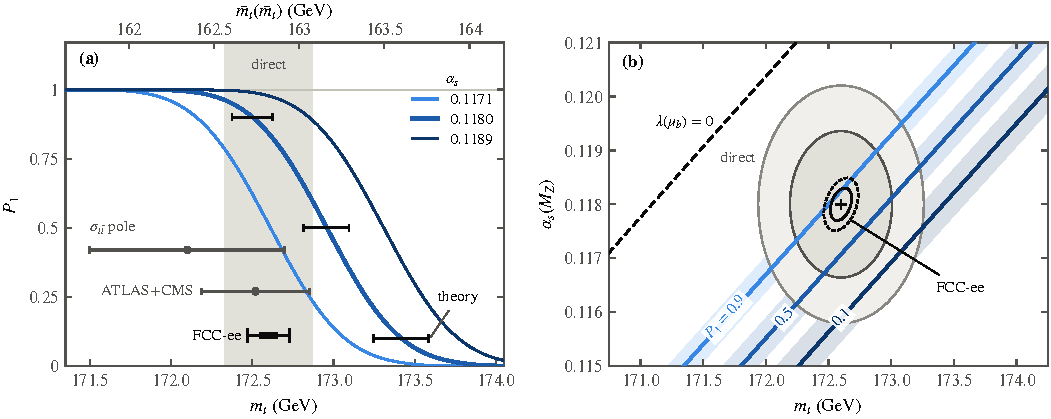
\includegraphics[width=\textwidth]{prd_criterion}
\caption{Top-mass criterion for survival.
(a)~Single-branch survival probability $\Pone(m_t)$ for $\alpha_s(M_Z)=0.1171$, $0.1180$ (thick), and $0.1189$, with theory $1\sigma$ bars (model, Standard Model mapping, $M_h$) at $\Pone=0.9$, $0.5$, and $0.1$.
Gray band: direct measurement; bars: $\sigma_{t\bar t}$ pole mass, ATLAS+CMS, and FCC-ee projection (thick: $m_t$; thin: total). %
Upper axis: $\mtbar$ at $\alpha_s=0.1180$.
(b)~Critical lines in the $(m_t,\alpha_s)$ plane with theory bands, the line $\lambda(\mub)=0$ (dashed), about $\mcMinusMzero\GeV$ below $\Pone=1/2$ (the absolute-stability line lies $0.10\GeV$ below it in $m_t$, Sec.~\ref{sec:rb-absstab}), and the $68\%$ and $95\%$ regions of present data and FCC-ee.} %
\label{fig:rb-criterion}
\end{figure}

\subsection{The absolute-stability line and the relative criterion}
\label{sec:rb-absstab}

The criterion is a statement about $\lambda$ at one scale, $\mub$, whereas the familiar stability bounds of the Standard Model concern the whole range of $\lambda(\mu)$.
To place it among them we computed, for this report, the absolute-stability line of the same mapping: the top pole mass $m_{\rm stab}$ at which
\begin{equation}
\min_{\mu\le\MPbar}\lambda(\mu)=0,
\label{eq:rb-absstab-def}
\end{equation}
with $\alpha_s(M_Z)=0.1180$ and $M_h=125.13\GeV$. %
The script \nolinkurl{higgs/01_sm_mapping/abs_stability.py} of the code package~\cite{DNECv12code} calls the Standard Model mapping of the main calculation, locates the minimum of $\lambda(\mu)$ on a logarithmic grid between $10^{8}\GeV$ and $\MPbar$, refines it with a bounded one-dimensional minimization in $\log_{10}\mu$, and solves for $m_{\rm stab}$ and $m_0$ with Brent's method; it writes \nolinkurl{abs_stability.json} next to itself.
We find
\begin{equation}
m_{\rm stab}=170.99\GeV\quad\bigl[\mtbar=161.29\GeV\bigr],\qquad m_0-m_{\rm stab}=0.10\GeV, %
\label{eq:rb-mstab}
\end{equation}
with the minimum of $\lambda(\mu)$ at $\mu=5.1\times10^{17}\GeV$, below $\MPbar$; the cut at the non-reduced Planck mass gives the same value. %
The script reproduces $m_0=171.0921\GeV$ (R5-029) to $2\times10^{-5}\GeV$ and $\lambda(\mub)$ at the central inputs to $4\times10^{-8}$, and a rerun with the research copy of the mapping gives identical values. %
At $\alpha_s=0.1171$ and $0.1189$ the line moves to $170.64$ and $171.34\GeV$, with $m_0-m_{\rm stab}=0.11$ and $0.09\GeV$. %
This number appears only in this report; the papers state only that the absolute-stability bound lies just below $m_0$~\cite{v12PRD,v12PRL}.

The ordering is therefore
\begin{equation}
m_{\rm stab}=170.99<m_0=171.09<m_c(\Pone=\tfrac12)=172.96\ll m_{\rm meta}=177.7\ \ {\rm GeV}, %
\label{eq:rb-ordering}
\end{equation}
where $m_{\rm meta}$ is the metastability bound of Ref.~\cite{Andreassen:2017rzq}, above which the electroweak vacuum of infinite flat space would have decayed in the age of the universe.
The finite-volume criterion lies $\mcMinusMzero\GeV$ above the line where $\lambda(\mub)$ changes sign and far below the metastability bound: a slightly negative quartic at $\mub$ is harmless, because the gauge zero-point energy confines the zero mode for the short duration of the turn. %
With our SMDR-type matching at the inputs of Ref.~\cite{Bednyakov:2015sca}, $M_h=125.7\GeV$ and $\alpha_s(M_Z)=0.1185$, the same script gives $171.47\GeV$, against $171.453\GeV$ with their own matching (Sec.~\ref{sec:rb-sm-bench}); the difference measures the matching scheme. %
In the relative form $m_c-m_0$ the criterion carries mainly the model error, because a shift of $\lambda(\mub)$ from the Standard Model mapping moves $m_c$ and $m_0$ together.

\subsection{Benchmarks and the change relative to fitted formulas}
\label{sec:rb-sm-bench}

From the matching formulas of Ref.~\cite{Buttazzo:2013uya} our running reproduces their couplings at the Planck scale: $g_1=0.61537$, $g_2=0.50546$, $g_3=0.48731$, $y_t=0.38245$, and $\lambda=-0.01436$, against $0.6154$, $0.5055$, $0.4873$, $0.3825$, and $-0.0143$. %
From the matching of Ref.~\cite{Bednyakov:2015sca} and for their inputs, $M_h=125.7\GeV$ and $\alpha_s(M_Z)=0.1185$, it reproduces their stability bound, $171.453\GeV$ at $\log_{10}(\mu/{\rm GeV})=17.750$ against $171.44\GeV$ and $17.752$. %
Two inputs of the fitted formulas differ from the full calculations.
The fitted $g_3(m_t)$ is $0.0017$--$0.0018$ higher than pure four-loop QCD, SMDR, and Ref.~\cite{Bednyakov:2015sca}, equivalent to $\Delta\alpha_s(M_Z)\approx+0.0004$, and the fitted $y_t(m_t)$ lacks the four-loop QCD term of the pole mass and is $0.00094$ too high. %

\begin{table}[t]
\centering
\caption{Change of the critical top mass at $\Pone=1/2$ when the earlier mapping (fitted matching, two-loop running, and a constant three-loop calibration of $\lambda$) is replaced by the mapping of this section, at $(m_t,\alpha_s)=(172.60\GeV,0.1180)$, converted with $d\lambda(\mub)/dm_t$.} %
\label{tab:rb-smchain}
\begin{tabular}{lcc}
\toprule
Step & $\lambda(\mub)$ & $\Delta m_c$ [GeV] \\
\midrule
Earlier mapping & $-0.0101929$ & \\ %
Five-loop running, no calibration & $-0.0103040$ & $-0.017$ \\ %
$g_3(m_t)$ from QCD & $-0.0110499$ & $-0.113$ \\ %
Four-loop QCD in $y_t(m_t)$ & $-0.0097062$ & $+0.203$ \\ %
SMDR matching & $-0.0097741$ & $-0.010$ \\ %
\midrule
Total & & $+0.063$ \\ %
\bottomrule
\end{tabular}
\end{table}

Table~\ref{tab:rb-smchain} decomposes the change relative to the earlier mapping.
The two corrections of the fitted inputs partly cancel, and the total, $+0.063\GeV$, is the same at all three levels of $\Pone$ to $0.002\GeV$ because the critical quartic at $\mub$ does not change. %
This is the step labelled NNLO in the refinement table of Sec.~\ref{rep:h-budget}.

\subsection{Top-mass definitions}
\label{sec:rb-mt-def}

With the same four-loop relation that enters the matching, the criterion reads $\mtbar<162.73$, $163.16$, and $163.60\GeV$ for $\Pone=0.9$, $0.5$, and $0.1$ at $\alpha_s(M_Z)=0.1180$, and $162.92$ and $163.41\GeV$ at $\Pone=1/2$ for $\alpha_s=0.1171$ and $0.1189$. %
The $\alpha_s$ dependence is $273\GeV$ per unit for $\mtbar$ against $387\GeV$ for the pole mass, about $30\%$ smaller, because part of the $\alpha_s$ dependence of $y_t(m_t)$ sits in the pole--$\MSbar$ relation. %
The $\mtbar$ form is free of the truncation of the pole series and of the renormalon ambiguity: the all-orders pole mass lies $0.272\GeV$ above our four-loop truncation, with an ambiguity of $0.07$--$0.11\GeV$~\cite{Beneke:2016cbu}. %

Top-mass definitions enter at the level of $0.5\GeV$~\cite{Butenschoen:2016lpz,Hoang:2020iah}. %
With the identification of assumption (A7), the direct (Monte Carlo) mass, $172.60\pm0.27\GeV$~\cite{ParticleDataGroup:2026mpi}, gives $\Pone=0.843$ at its central value. %
The cross-section pole mass, $172.1\pm0.6\GeV$~\cite{ParticleDataGroup:2026mpi}, gives $\Pone=0.99$, and the ATLAS+CMS combination, $172.52\pm0.33\GeV$~\cite{ATLAS:2024dxp}, gives $0.89$. %
For the direct mass we follow Ref.~\cite{Hoang:2020iah}: either it is identified with the pole mass with an interpretation error of $0.5\GeV$, or it is identified with the MSR mass at $1.3\GeV$, which lies $0.36\pm0.25\GeV$ below the pole mass~\cite{Hoang:2017suc}. %
Calibrations of the Monte Carlo against $e^+e^-$ event shapes support an interpretation error of this size~\cite{Butenschoen:2016lpz}.
The MSR identification puts the measured direct mass at a pole-mass equivalent of $172.96\GeV$, at the criterion itself, and gives $\Pbar=\PbarMSR$ (Sec.~\ref{rep:h-budget}). %

\subsection{Theory error of the mapping}
\label{sec:rb-sm-error}

The matching-scale dependence is the leading theory error, and three ways of estimating it differ by an order of magnitude.
(i)~Varying all evaluation scales of the compiled SMDR fit together by factors $\frac12$ and $2$ moves $m_c$ by $+0.033$ and $-0.019\GeV$. %
This small value comes from a cancellation: the top-mass scale alone gives $+0.067$ and $-0.027\GeV$, and the Higgs-mass scale $-0.037$ and $+0.011\GeV$. %
At two-loop accuracy for $M_h$ the Higgs-mass term doubles, to $-0.070$ and $+0.030\GeV$, while the common variation shrinks to $+0.006$ and $+0.002\GeV$, so the smallness reflects cancellation rather than convergence. %
Varying each scale independently gives the envelope $[-0.069,+0.082]\GeV$. %
(ii)~The two-loop fixed-order matching in the $G_F$ scheme~\cite{Bednyakov:2015sca,Kniehl:2016enc}, recomputed blind with the library mr, moves $m_c$ by $+0.173\GeV$ for $\mu_0=m_t/2$ and $-0.358\GeV$ for $\mu_0=2m_t$, reproducing the published scale variation of the stability bound. %
Decomposed linearly, $y_t$ contributes $+0.136/-0.196\GeV$, of which the pure-QCD tower is $+0.055/-0.066\GeV$, and $\lambda$ contributes $+0.037/-0.162\GeV$; the gauge couplings contribute less than $0.004\GeV$. %
In that scheme the non-QCD logarithms of $\lambda$ and $y_t$ are large and of the same sign; they, and not the tadpoles, cause the larger spread, since the tadpole contributions cancel identically in the coefficients used there.
(iii)~A reconstruction of the missing three-loop logarithms from the renormalization group, which we used before compiling SMDR, gives $[-0.088,+0.102]\GeV$ and overestimates the full calculation by about a factor of three. %

We adopt the following budget.
For the matching scale we take the independent variation of the SMDR evaluation scales, with the pure-QCD tower removed from the top-mass scale, $[-0.042,+0.054]\GeV$; it does not rely on the cancellation of (i). %
For the organization of the fixed-order result we take the difference between mr and SMDR at $\mu_0=m_t$, $0.042\GeV$, a direct calculation that includes the leading three-loop terms of SMDR ($0.014\GeV$). %
The truncation of the running ($0.005\GeV$), the order of the $\alpha_s$ input ($0.003\GeV$), and the $W$ and $Z$ pole-mass convention ($0.011\GeV$) are small. %
In quadrature these give $\pm0.070\GeV$ for $\mtbar$. %
The pole form adds $0.075\GeV$ for the uncomputed $O(\alpha_s^5)$ term of Eq.~(\ref{eq:rb-zm}), a geometric extrapolation that agrees with the scale variation of the pure-QCD tower and with the renormalon ambiguity; these are the same order and are counted once. %
The total for the pole form is $\pm0.102\GeV$. %
The $G_F$-scheme spread of (ii), $+0.17/-0.36\GeV$ in $m_c$, enters only as a robustness variant, with $\Pbar=\PbarBKPV$ depending on how its asymmetric errors are combined (Sec.~\ref{rep:h-budget}). %

The parametric errors are kept separate.
$M_h=125.13\pm0.11\GeV$ moves $m_c$ by $\pm0.053\GeV$, and $\alpha_s(M_Z)=0.1180\pm0.0009$ by $\pm0.35\GeV$ ($\pm0.25\GeV$ for $\mtbar$). %
Using $M_h=125.20\GeV$ instead would raise $m_c$ by $0.034\GeV$. %
The scale variation estimates the three-loop electroweak and mixed threshold corrections at $\mu_0$.
Assumption (A2) takes the Standard Model to hold up to $\mub$; new states below $\mub$ that couple to the Higgs would change $\lambda(\mub)$, and the criterion tests the Standard Model up to that scale.

\subsection{Independent mapping}
\label{sec:rb-sm-blind}

An independent mapping was written from the published conventions alone, without access to our code, using mr~1.3.2~\cite{Kniehl:2016enc} for the matching and its three-loop $\beta$ functions (Sec.~\ref{rep:v-blind}).
Its 276 three-loop monomials agree with the appendix of Ref.~\cite{Buttazzo:2013uya} one by one, and numerically with the SMDR $\beta$ functions to $10^{-15}$. %
With the SMDR matching its quartic at $\mub$ differs from ours by $4\times10^{-6}$, equivalent to $0.0006\GeV$, and its $y_t$ by $2\times10^{-6}$. %
With the mr matching it is lower by $2.8\times10^{-4}$, or $0.043\GeV$, which is the scheme item of the budget. %
The library mr must run single-threaded; its OpenMP sections otherwise give nondeterministic two-loop integrals.
The blind check also compiled SMDR independently and reproduced our scale variations of (i) exactly, so the differences between (i) and (ii) are traced to their source and not to an implementation.

\section{Error budget, marginalization and experimental reach}\label{rep:h-budget}

This section collects the uncertainties of the critical top mass, combines them with the measured inputs into a survival probability, and asks what present and future measurements can decide.
We find that the model error at $\Pone=1/2$ is $^{+\modelErrUp}_{-\modelErrDn}\GeV$, dominated by the inflation scale, which enters through the duration of the turn; without that item it is $^{+\modelErrUpNoVi}_{-\modelErrDnNoVi}\GeV$, comparable to the Standard Model theory error. %
The parametric error from $\alpha_s$, $\pm0.35\GeV$, exceeds the theory and model errors combined; of all the items only the Monte Carlo--pole interpretation of the measured mass, $\pm0.5\GeV$, is larger. %
Marginalizing over the measured masses, $\alpha_s$, and the theory and model errors gives a survival probability $\Pbar=\PbarOne$ for the direct top mass ($\PbarMSR$ to $\PbarSigma$ across top-mass definitions), provided the Higgs curvature coupling satisfies $\xiH(\mub)\gtrsim\xiHmin$ (Sec.~\ref{rep:h-universality}). %
The survival probability is not evidence for this beginning: for all measurements, mass definitions and priors the Bayes factors obey $|\ln B|\le\BayesMax$. %
A top-quark pole mass above $\mExclFCC\GeV$, within reach of FCC-ee, would establish $\Pone<0.1$ at $95\%$ confidence; at the threshold the central $\Pone$ is $\approx\PoneAtExclFCC$ and the Bayes factor $B_{\rm ex}\approx\BexFCC$. %

\subsection{Refinements of the model}
\label{sec:rb-convergence}

Table~\ref{tab:rb-convergence} follows the critical mass through the refinements of the model, all with the same hazard procedure at $\alpha_s(M_Z)=0.1180$. %
The first five steps (rows 2--6) add distinct physical effects, not successive orders of one expansion: the $\MSbar$ continuum term of the matching, the Coulomb-gauge counting (Sec.~\ref{rep:h-matching}), the exact gauge shape from DMC, and the joint dynamics of the hypercharge mode (Sec.~\ref{rep:h-reduced}).
Each moves $m_c$ by $0.04$ to $0.11\GeV$ toward larger values. %
The last of these, the DMC shape in two dimensions, was first obtained by converting width ratios; a calibrated one-dimensional hazard and direct two-dimensional roots at every node change $m_c$ by only $0.011$ and $0.001\GeV$, so the numerical implementation of the reduced model has converged. %
The NNLO mapping of Sec.~\ref{rep:h-smmap} then shifts all levels by $+0.063\GeV$ through $\lambda(\mub;m_t)$ alone. %
The cross terms of Sec.~\ref{rep:h-cross} are the first refinement that lowers $m_c$, and their final one-loop terms move it back by $+0.005$ to $+0.007\GeV$; the row with the anticommutator vertex is an intermediate step whose vertex the background-covariant one replaces (Sec.~\ref{sec:rb-r2c2}). %
Figure~\ref{fig:rb-cross}(b) shows the same sequence.

\begin{table}[t]
\centering
\caption{Critical top mass (GeV) at $\Pone=0.9$ and $1/2$ through the refinements of the model, and the shift of each step at $\Pone=1/2$, at $\alpha_s(M_Z)=0.1180$.
Rows above the NNLO step use the earlier Standard Model mapping.
The vertex row uses the anticommutator vertex of ordinary Coulomb gauge; the final row adds the background-covariant vertex and the Coulomb mismatch.} %
\label{tab:rb-convergence}
\begin{tabular}{lccc}
\toprule
Stage & $\Pone=0.9$ & $\Pone=0.5$ & Shift \\
\midrule
Unitary, $D_\theta$ only & $172.210$ & $172.584$ & \\ %
$+\,V_{\rm CW}$ & $172.276$ & $172.656$ & $+0.072$ \\ %
Coulomb gauge & $172.348$ & $172.768$ & $+0.112$ \\ %
1D $+$ DMC shape & $172.393$ & $172.831$ & $+0.063$ \\ %
2D, Gaussian shape & $172.467$ & $172.941$ & $+0.110$ \\ %
2D $+$ DMC (rescaled) & $172.509$ & $173.002$ & $+0.061$ \\ %
Calibrated 1D hazard & $172.517$ & $173.013$ & $+0.011$ \\ %
2D direct, all nodes & $172.518$ & $173.014$ & $+0.001$ \\ %
$+$ NNLO mapping & $172.583$ & $173.078$ & $+0.063$ \\ %
$+$ cross terms (CCA) & $172.498$ & $172.954$ & $-0.124$ \\ %
$+$ vev, top vertices & $172.495$ & $172.950$ & $-0.003$ \\ %
$+$ Coulomb (final) & $172.502$ & $172.960$ & $+0.009$ \\ %
\bottomrule
\end{tabular}
\end{table}

\subsection{The error budget}
\label{sec:rb-table}

Table~\ref{tab:rb-budget} is the error budget of the critical mass, the de-duplicated rebuild of the final model.
Each model item is computed in the final model or converted with its hazard slopes, $d\ln I/dm_t=5.269$, $3.218$, and $2.121\GeV^{-1}$ at $\Pone=0.9$, $0.5$, and $0.1$; the entries at $\Pone=0.1$ are therefore computed rather than extrapolated. %
Model items are combined in quadrature on each side; one-sided items carry their sign.

\begin{table}[t]
\centering
\caption{Error budget for the critical top-quark mass $m_c$ at which $\Pone$ takes the value in the column header, for $\alpha_s(M_Z)=0.1180$ and $M_h=125.13\GeV$ (entries in GeV). %
The first row gives $m_c$ for the pole mass and, in brackets, for $\mtbar$.
The Standard Model mapping and $\alpha_s$ rows give the pole and [$\mtbar$] forms; the other rows are pole-mass shifts, which differ from their $\mtbar$ counterparts by about $5\%$. %
Robustness variants not included: all-orders pole mass $+0.27$ (one-sided), renormalon ambiguity $0.07$--$0.25$, tadpole-including scale variation $+0.17/-0.36$, and $\rT=10^{-4}$ ($-0.09$, $-0.17$, $-0.28$).} %
\label{tab:rb-budget}
\small\setlength{\tabcolsep}{4pt}
\begin{tabular}{lcccc}
\toprule
 & $\Pone=0.9$ & $\Pone=0.5$ & $\Pone=0.1$ & Sec. \\
\midrule
$m_c$ [$\bar m_c$] & $172.50$ [$162.73$] & $172.96$ [$163.16$] & $173.42$ [$163.60$] & \ref{rep:h-smmap} \\ %
Reduced model: residual DMC shape & $\pm0.002$ & $\pm0.002$ & $\pm0.002$ & \ref{rep:h-reduced} \\ %
One-loop matching ($\mu$, top threshold) & $^{+0.009}_{-0.039}$ & $^{+0.012}_{-0.049}$ & $^{+0.015}_{-0.058}$ & \ref{rep:h-matching} \\ %
Cross terms, model-internal & $\pm0.008$ & $\pm0.010$ & $\pm0.013$ & \ref{rep:h-cross} \\ %
Cross terms, blind recalculation & $\pm0.004$ & $\pm0.007$ & $\pm0.010$ & \ref{rep:h-cross} \\ %
Full-dimensional validation (one-sided) & $+0.012$ & $+0.020$ & $+0.031$ & \ref{rep:h-reduced} \\ %
Numerics & $\pm0.002$ & $\pm0.002$ & $\pm0.002$ & \ref{rep:h-reduced} \\ %
Inflation scale, $\rT\in[10^{-3},10^{-2}]$ & $\pm0.035$ & $\pm0.067$ & $\pm0.112$ & \ref{rep:h-budget} \\ %
Preparation weight $w_0$ (one-sided) & $-0.016$ & $-0.006$ & $-0.004$ & \ref{rep:h-survival} \\ %
Model total & $^{+\modelErrUpPnine}_{-\modelErrDnPnine}$ & $^{+\modelErrUp}_{-\modelErrDn}$ & $^{+\modelErrUpPone}_{-\modelErrDnPone}$ & \\[2pt] %
\quad without inflation scale & $^{+\modelErrUpNoViPnine}_{-\modelErrDnNoViPnine}$ & $^{+\modelErrUpNoVi}_{-\modelErrDnNoVi}$ & $^{+\modelErrUpNoViPone}_{-\modelErrDnNoViPone}$ & \\[2pt] %
\midrule
Standard Model mapping, pole [$\mtbar$] & $\pm0.10$ [$\pm0.07$] & $\pm0.10$ [$\pm0.07$] & $\pm0.10$ [$\pm0.07$] & \ref{rep:h-smmap} \\ %
$\alpha_s(M_Z)\pm0.0009$ & $\pm0.35$ [$\pm0.25$] & $\pm0.35$ [$\pm0.25$] & $\pm0.35$ [$\pm0.25$] & \ref{rep:h-smmap} \\ %
$M_h\pm0.11\GeV$ & $\pm0.053$ & $\pm0.053$ & $\pm0.053$ & \ref{rep:h-smmap} \\ %
Measurement of $m_t$ (direct) & $\pm0.27$ & $\pm0.27$ & $\pm0.27$ & \ref{rep:h-smmap} \\ %
Monte Carlo--pole interpretation & $\pm0.5$ & $\pm0.5$ & $\pm0.5$ & \ref{rep:h-smmap} \\ %
\bottomrule
\end{tabular}
\end{table}

\paragraph{Content of the model items.}
\emph{Reduced model.}
The earlier estimate of the reduction error had four parts: the $\pm1\sigma$ uncertainty of the DMC shape correction, the $x$-sector Born--Huang term, the transfer of width ratios computed at fixed couplings, and the difference between static and hazard conversions.
The full-dimensional comparison of Sec.~\ref{sec:rb-fulldim} measures the first two directly, and the node-direct hazard has no ratio transfer and no static conversion.
What remains is the use of fixed couplings in $\delta E_{\rm DMC}$, estimated at $\pm0.002\GeV$. %
\emph{Matching.}
The scale scan of Sec.~\ref{sec:rb-scale} gives $^{+0.009}_{-0.039}$, $^{+0.012}_{-0.049}$, and $^{+0.015}_{-0.058}\GeV$; it is asymmetric because the conservative range $c\in[\frac12,2\pi]$ extends upward beyond the natural scale $\mu_*=3.41/L$. %
\emph{Cross terms.}
The two cross-term items are the model-internal error of Table~\ref{tab:rb-xerr} and, separately, the difference between the blind and main calculations of the dominant part (Sec.~\ref{sec:rb-xfinal}).
\emph{Full-dimensional validation.}
This item is the one-sided WKB envelope of Sec.~\ref{sec:rb-fulldim}, $+0.012$, $+0.020$, and $+0.031\GeV$. %
\emph{Numerics.}
The numerical item, $\pm0.002\GeV$, covers the node set, the discretization, the root windows, and the order of the outgoing-wave condition (Sec.~\ref{sec:rb-nodes}). %
\emph{Inflation scale.}
This item varies the tensor-to-scalar ratio over $\rT\in[10^{-3},10^{-2}]$ in the plateau family at fixed scalar amplitude (assumption (A3)); its derivation follows. %
\emph{Preparation.}
This item consists of the one-sided shifts from the minimal-variance weight, $-0.016$, $-0.006$, and $-0.004\GeV$ (Sec.~\ref{sec:rb-w0}). %

\subsection{The background of the turn and the inflation scale}
\label{sec:rb-background}

The background of the turn enters the Higgs calculation only through two numbers.
The turning solution, $3\MPbar^2h^2=C_{\rm eff}/\Lb^4$ with $a^2=\cosh2\tau$, is an exact scaling solution (Sec.~\ref{rep:turning}).
A change of an input therefore acts only through the matching scale and the duration, $\delta_\mu=\Delta\ln\mub=-\Delta\ln\Lb$ and $\delta_h=\Delta\ln(h\Lb)$.
Taking the logarithm of the turning condition, $4\,\Delta\ln\Lb=\Delta\ln C_{\rm eff}-2\Delta\ln h$, so that
\begin{align}
\delta_\mu&=-\tfrac14\Delta\ln C_{\rm eff}+\tfrac12\Delta\ln h,\nonumber\\
\delta_h&=+\tfrac14\Delta\ln C_{\rm eff}+\tfrac12\Delta\ln h,
\label{eq:rb-background}
\end{align}
and the hazard becomes
\begin{equation}
I=\int_0^5\frac{\Gamma\bigl(m_t,\ell(\tau)+\delta_\mu\bigr)\,d\tau}{h\Lb\,e^{\delta_h}(\cosh2\tau)^{1/2}},\qquad \ell(\tau)=-\tfrac12\ln\cosh2\tau,
\label{eq:rb-Ishift}
\end{equation}
where $\ell=\ln(\mu/\mub)$ labels the scale of the node couplings.
We compute $\Gamma$ at the eleven nodes and at three further scales with recomputed gauge profiles and interpolate in $\ell$; four direct reruns with all nodes shifted agree with the interpolation to $1.1\times10^{-7}\GeV$. %

For the plateau the scale obeys $h\propto(A_s\rT)^{1/2}$ at fixed scalar amplitude $A_s$, so a change of $\rT$ gives $\delta_\mu=\delta_h=\frac14\Delta\ln\rT$.
With $d\ln I/d\lambda(\mub)=-805$, $-488$, and $-319$ at the three levels, $\rT\in[10^{-3},10^{-2}]$ gives the inflation-scale item $\pm0.035$, $\pm0.067$, and $\pm0.112\GeV$, and $\rT=10^{-4}$ gives $-0.089$, $-0.173$, and $-0.280\GeV$. %
The dominant continuous input is the duration of the turn: changing $h\Lb$ by a factor $e^{\pm1}$ moves $m_c$ by $+0.214$ and $-0.170\GeV$ at $\Pone=0.9$ and by $+0.367$ and $-0.270\GeV$ at $\Pone=1/2$, consistent with the local derivative $dm_c/d\ln\eta_\infty=-0.31\GeV$ at $\Pone=1/2$ (Sec.~\ref{rep:h-universality}) and the curvature of $\ln I(m_t)$. %
Inputs that change the matter content of the turn move $m_c$ by at most $0.009\GeV$: the zero-mode share $\fzm=0.28$, $0.258$, or $0.308$, an inflaton or three right-handed neutrinos through their Casimir weight alone, the next-order zero-mode energy, $A_s$ within $1\sigma$, the shape stiffness, and the $1\%$ difference between the Higgs-calculation value $h/\MPbar=6.054\times10^{-6}$ and the instantaneous-reheating value $6.116\times10^{-6}$. %
A reheating history with weak visible decay changes $m_c$ by $+0.013\GeV$ at $\Pone=1/2$, inside the inflation-scale item. %

\subsection{Combination}
\label{sec:rb-combination}

The total at $\Pone=1/2$ is $^{+\modelErrUp}_{-\modelErrDn}\GeV$, and $^{+\modelErrUpNoVi}_{-\modelErrDnNoVi}\GeV$ without the inflation-scale item; at $\Pone=0.9$ and $0.1$ it is $^{+\modelErrUpPnine}_{-\modelErrDnPnine}$ and $^{+\modelErrUpPone}_{-\modelErrDnPone}\GeV$. %
Two items may overlap and are both kept, which errs on the conservative side: the blind-versus-main difference of the cross terms and the first-order-versus-variational part of their model-internal error.
The inflation-scale item was computed with the cross terms before their final one-loop corrections; scaling with the hazard slopes changes it by at most $0.001\GeV$. %
Rebuilding the budget changed the totals by at most $0.002\GeV$ relative to the earlier compilation, and the marginalized probability by $2\times10^{-4}$. %
The model total is thus smaller than each of the parametric errors of $\alpha_s$, the measured mass, and its interpretation.

\subsection{Marginalized survival probability}
\label{sec:rb-pbar}

The probability that the zero mode survives, given current data, is
\begin{equation}
\Pbar=\int\Pone\bigl(m_t,\alpha_s,M_h;\delta_{\rm SM},\delta_{\rm mod}(Z)\bigr)\,dP(m_t)\,dP(\alpha_s)\,dP(M_h)\,dP(\delta_{\rm SM})\,dP(Z),
\label{eq:rb-Pbar}
\end{equation}
with Gaussian measurement and Standard Model errors.
The asymmetric model error is carried by one nuisance parameter $Z\sim\mathcal N(0,1)$, coherent across the levels of $\Pone$, with $\delta_{\rm mod}=\sigma_+Z$ for $Z>0$ and $\sigma_-Z$ for $Z<0$, so that the central value is the median; $\sigma_\pm$ are interpolated between the levels.

\paragraph{Surface.}
We evaluate Eq.~(\ref{eq:rb-Pbar}) on a surface $\Pone(m_t,\alpha_s)$ built from the ten-point grid of Sec.~\ref{sec:rb-hazard} at $\alpha_s=0.1180$ and the critical masses at three levels for $\alpha_s=0.1171$, $0.1180$, and $0.1189$. %
For the outer values of $\alpha_s$ we map the masses of the central grid level by level, quadratically in $m_t-m_c(\Pone=1/2)$, keep $\ln I$, and interpolate quadratically in $\alpha_s$.
Direct hazards from the node widths at $\alpha_s=0.1171$ and $0.1189$, five masses each, agree with the surface to $|\Delta\Pone|\le4.4\times10^{-4}$. %

\paragraph{Asymmetric errors.}
For asymmetric errors we use an equal-mass split: the shift is $+\sigma_+|Z|$ or $-\sigma_-|Z|$ with probability $\frac12$ each, so the central value is the median and $\pm\sigma_\pm$ are the $16\%$ and $84\%$ points.
This preserves the meaning of the asymmetric inputs, which are $68\%$ ranges or envelopes about a central value; a continuous two-piece normal would move the mean, for the tadpole-including variant by $(2/\pi)^{1/2}(\sigma_+-\sigma_-)=-0.15\GeV$. %
Using continuous two-piece normals throughout lowers $\Pbar$ by $0.0025$. %

\paragraph{Results.}
For the direct mass $\Pbar=\PbarOne$; the central $68\%$ interval of $\Pone$ is $[\PbarQlo,\PbarQhi]$, and $\Pone\ge1/2$ with probability $\PbarGeHalf$. %
Adding the errors one at a time, the measurement of $m_t$ lowers $\Pbar$ from the curve value $0.843$ by $0.054$, $\alpha_s$ by a further $0.052$, $M_h$ and the Standard Model mapping by $0.004$ together, and the model error changes it by $-0.003$, because its two sides nearly balance; a $0.5\GeV$ interpretation error lowers it by $0.050$. %
The result depends on how the measured mass is interpreted: $\Pbar=\PbarInterp$ with a $0.5$-GeV Monte Carlo--pole interpretation error, $\PbarSigma$ for the cross-section pole mass, and $\PbarMSR$ for the MSR identification. %
For the other measurements $\Pbar=\PbarATLASCMS$ (ATLAS+CMS), $\PbarCMS$ (CMS), and $\PbarMbarSigma$ for the $\MSbar$ cross-section value $162.5^{+2.1}_{-1.5}\GeV$. %
Expressing the direct mass as $\mtbar$ gives the same value as the pole form, because the identification ambiguity of the direct mass returns on the measurement side; the $\mtbar$ form gains only for short-distance measurements such as a threshold scan. %
The tadpole-including Standard Model variant gives $\Pbar=\PbarBKPV$, depending on how its asymmetric errors are combined. %

\paragraph{Independent integration.}
An independently written direct Monte Carlo integration, which shares no code with the quadrature and uses a different surface (monotone cubic interpolation in $\ln(-\ln\Pone)$ with clamped $\alpha_s$ offsets) and $4\times10^6$ samples per definition, agrees with it to $5\times10^{-4}$ for all eleven definitions. %
The probability $P(\Pone\ge\frac12)$ differs by $0.005$ between the two codes because one assigns the model width at the threshold level and the other at the unshifted sample; both round to $\PbarGeHalf$. %
A blind marginalization with the earlier model is described in Sec.~\ref{rep:v-blind}.

\subsection{Bayes factors}
\label{sec:rb-bayes}

The survival probability is not evidence for this beginning.
We compare the hypothesis that the zero mode survived with the same hypothesis without the survival requirement through
\begin{equation}
B_{\rm ex}=\Pbar,\qquad B_{\rm sel}=\frac{\Pbar}{\langle\Pone\rangle_{\rm prior}},
\label{eq:rb-bayes}
\end{equation}
where $B_{\rm ex}\le1$ is the exclusion factor, the probability that the data leave the beginning viable, and $B_{\rm sel}$ asks whether the measured masses select the surviving region more often than a broad prior would.
The priors are flat in $m_t$ on $[150,200]\GeV$ or $[170,176]\GeV$, or flat in $\lambda(\mub)$. %
For the direct mass $B_{\rm sel}=\BselDirect$ for the first prior, against an upper bound $1/\langle\Pone\rangle_{\rm prior}=\BselMax$, and $1.48$ and $1.17$ for the other two. %
Over all measurements, mass definitions and priors $B_{\rm ex}$ lies between $0.61$ and $0.97$ and $B_{\rm sel}$ between $0.98$ and $2.11$, so $|\ln B|\le\BayesMax$: current data neither favor nor disfavor this beginning. %
In particular, the fact that the measured mass lies near the critical line is not evidence.

\subsection{Exclusion and experimental reach}
\label{sec:rb-reach}

On the central curve $\Pone<0.1$ for $m_t>173.42\GeV$, and $173.07$ or $173.77\GeV$ for $\alpha_s$ one standard deviation lower or higher. %
With the Standard Model, $M_h$, and model errors folded in, but without the $\alpha_s$ and measurement errors, $\Pone<0.1$ at $95\%$ confidence for $m_t>\mExclTheory\GeV$. %
With the present measurement error of $0.27\GeV$ and $\alpha_s$ marginalized, a $95\%$ exclusion would need a measured central value of $\mExclMeas\GeV$, or $\mExclMeasInterp\GeV$ with a $0.5\GeV$ interpretation error. %

Future measurements can decide.
We fold the projected errors with the Standard Model error of the $\mtbar$ form and the model error.
FCC-ee threshold scans aim at $\delta\mtbar=50\,\mathrm{MeV}$ with $\delta\alpha_s=0.0002$~\cite{Freitas:2019bre,FCC:2025lpp}, a total error of $0.131\GeV$. %
They would separate true masses of $172.6$ and $173.3\GeV$ at $\sigFCC\sigma$, establish the surviving side for a measured value below $172.74\GeV$, and establish $\Pone<0.1$ at $95\%$ confidence for a measured pole mass above $\mExclFCC\GeV$; at the threshold the central $\Pone$ is $\approx\PoneAtExclFCC$ and the Bayes factor of Eq.~(\ref{eq:rb-bayes}) is $B_{\rm ex}\approx\BexFCC$, and both are smaller above it. %
With $38\,\mathrm{MeV}$ and $\delta\alpha_s=0.0001$ the separation is $6.0\sigma$. %
At the HL-LHC, with $\delta m_t=0.17\GeV$~\cite{Azzi:2019yne}, a pole-mass determination separates the two masses at $1.71\sigma$, $2.54\sigma$, or $3.08\sigma$ for $\delta\alpha_s=0.0009$, $0.00045$, or $0.0002$, that is $\sigHLLHCmin\sigma$ for the present $\alpha_s$ and $\sigHLLHCmax\sigma$ if lattice determinations halve its error~\cite{FCC:2025lpp}; the gain comes almost entirely from $\alpha_s$. %
For the direct mass with its $0.5\GeV$ interpretation uncertainty the separation is $1.08\sigma$, $1.23\sigma$, or $1.27\sigma$ for the same three values of $\delta\alpha_s$, that is $\sigHLLHCinterpMin$--$\sigHLLHCinterpMax\sigma$ for the present and the halved $\alpha_s$ error. %
Today the separation is $1.5\sigma$. %

\section{Universality and the curvature coupling}\label{rep:h-universality}

The threshold $\lamc\approx-0.01$ does not depend on the details of one point in parameter space, and its use as a survival criterion requires a condition on the Higgs curvature coupling.
We show that the duration of the turn enters only logarithmically, that the couplings enter with logarithmic derivatives below $0.7$, and that sectors with 't~Hooft flux cannot turn around. %
A finite threshold exists in every sector that can host a turning point and keeps a Higgs zero mode, because there the zero-point motion of the constant gauge modes still confines the zero mode, so that for $\lambda<0$ it is a resonance and a finite duration gives a finite threshold (Sec.~\ref{sec:rb-spin}); we compute $\lamc\approx-0.01$ for the AAA structure, and an indicative estimate gives a threshold of the same size for the PPA and PAA structures. %
For the curvature coupling we find that the survival probability stays within $1\%$ of its conformal value for $\xiH(\mub)\gtrsim\xiHcentral$ at the measured top mass, or $\gtrsim\xiHmin$ including all prescription variants ($\approx\xiHminEW$ at the electroweak scale), and for $\xiH(\mub)\gtrsim\xiHhalf$ at the point $\Pone=1/2$. %
This zero-mode condition is stronger than the all-mode bound from the subsequent inflation for $m_t\gtrsim172.1\GeV$, and the conformal value $\xiH=1/6$ satisfies both. %

\subsection{Duration of the turn}
\label{sec:rb-duration}

Changing only the duration of the turn at fixed $\Lb$ (that is, changing $h$) leaves $\mub$ and every node coupling unchanged, so $\Gamma(\tau)$ is unchanged and $\eta_\infty\to f\eta_\infty$ is exactly equivalent to $I\to fI$ in Eq.~(\ref{eq:rb-hazard}).
Near threshold the width has the WKB form of Sec.~\ref{sec:rb-size}, $I\simeq A_{\rm eff}\eta_\infty\exp(-b_{\rm eff}|\lambda|^{-1/2})$ with $\lambda\equiv\lambda(\mub)$.
Holding $I$ fixed at the value that defines a level of $\Pone$, $\ln\eta-b_{\rm eff}|\lamc|^{-1/2}$ is constant, so
\begin{align}
|\lamc(\eta)|^{-1/2}&=|\lamc(\eta_0)|^{-1/2}+\frac{\ln(\eta/\eta_0)}{b_{\rm eff}},\nonumber\\
\frac{d\lamc}{d\ln\eta_\infty}&=\frac{2|\lamc|^{3/2}}{b_{\rm eff}},\qquad
\frac{dm_c}{d\ln\eta_\infty}=-\frac{2|\lamc|^{3/2}}{b_{\rm eff}\,|d\lambda(\mub)/dm_t|},
\label{eq:rb-eta}
\end{align}
where the last relation uses $\lamc\equiv\lambda_{\rm SM}(\mub;m_c)$ and Eq.~(\ref{eq:rb-lin}).
With $b_{\rm eff}=1.40$, $1.30$, and $1.19$ this gives $dm_c/d\ln\eta_\infty=-0.19$, $-0.31$, and $-0.47\GeV$ at $\Pone=0.9$, $0.5$, and $0.1$; equivalently $|\lamc|\propto\eta_\infty^{-0.137}$, $\eta_\infty^{-0.170}$, and $\eta_\infty^{-0.208}$. %

\begin{table}[t]
\centering
\caption{Hazard-equivalent threshold $\lamc(\mub)$ when the conformal duration is changed to $f\eta_\infty$ at fixed node widths (earlier model).
The entries for $f=0.25$, $\Pone=0.1$ and $f=4$, $\Pone=0.9$ use a linear extrapolation of $\ln I$ beyond the mass grid by at most $0.2\GeV$.} %
\label{tab:rb-eta}
\begin{tabular}{cccc}
\toprule
$f$ & $\Pone=0.9$ & $\Pone=0.5$ & $\Pone=0.1$ \\
\midrule
$0.25$ & $-0.011156$ & $-0.015745$ & $-0.020655$ \\ %
$0.5$ & $-0.010039$ & $-0.013698$ & $-0.017672$ \\ %
$1$ & $-0.009104$ & $-0.012104$ & $-0.015140$ \\ %
$2$ & $-0.008306$ & $-0.010820$ & $-0.013233$ \\ %
$4$ & $-0.007618$ & $-0.009759$ & $-0.011734$ \\ %
\bottomrule
\end{tabular}
\end{table}

Table~\ref{tab:rb-eta} gives the direct recalculation.
Equation~(\ref{eq:rb-eta}) agrees with it to $0.6\%$ when $\eta_\infty$ changes by a factor of 2 and to $1.3\%$ for a factor of 4; its only error is the $\lambda$ dependence of the local exponent, a second-order effect. %
Halving or doubling the duration moves $m_c$ by $+0.24$ or $-0.20\GeV$ at $\Pone=1/2$ ($+0.14/-0.12$ and $+0.38/-0.29\GeV$ at $\Pone=0.9$ and $0.1$). %
An independent full-chain recalculation with $h\Lb$ changed by $e^{\pm1}$, in which $\mub$ and the node couplings move as well, agrees with Eq.~(\ref{eq:rb-eta}) to $1$--$3\%$ (Sec.~\ref{sec:rb-background}). %
The magnitude of $\lamc$ follows from Eq.~(\ref{eq:rb-lamc-size}): doubling or halving $\eta_\infty$ changes $|\lamc|$ by $-11\%$ or $+13\%$. %

\subsection{Dependence on the couplings}
\label{sec:rb-couplings}

We multiply the node couplings by $1\pm0.1$ at fixed $\lambda(\mu)$, one coupling at a time, recompute the Gaussian profiles, the matching, the cross terms, and the two-dimensional roots at five nodes and five masses, and convert the width ratios into hazards.
This study uses the earlier model; for unit multipliers the variant code reproduces its roots to $5\times10^{-12}$ in $\Gamma$, and the $+10\%$ and $-10\%$ sides are symmetric to within $5\%$. %
At $\Pone=1/2$ we find
\begin{equation}
\frac{\partial\ln|\lamc|}{\partial\ln g_2}=0.66,\qquad \frac{\partial\ln|\lamc|}{\partial\ln g_Y}=0.16,\qquad \frac{\partial\ln|\lamc|}{\partial\ln y_t}=0.63, %
\label{eq:rb-coupderiv}
\end{equation}
nearly the same at $0.9$ and $0.1$ for $g_2$ and $g_Y$, and within $10\%$ for $y_t$ ($0.575$, $0.627$, $0.649$). %
Increasing any of the three couplings makes $\lamc$ more negative and the zero mode more stable.
Locally,
\begin{equation}
|\lamc|\approx0.0121\Bigl(\frac{\eta_\infty}{300}\Bigr)^{-0.17}\Bigl(\frac{g_2}{0.528}\Bigr)^{0.66}\Bigl(\frac{g_Y}{0.443}\Bigr)^{0.16}\Bigl(\frac{y_t}{0.430}\Bigr)^{0.63}, %
\label{eq:rb-powerlaw}
\end{equation}
with the couplings taken at the first node; larger changes should use the logarithmic form of Eq.~(\ref{eq:rb-eta}).

\paragraph{WKB decomposition.}
The same structure explains these exponents.
Write the hazard as $I=A\,e^{-b|\lambda|^{-1/2}}$, where $A$ and $b$ depend on a coupling $g_i$.
The sensitivity at fixed $\lambda$ is then $s_i\equiv\partial\ln I/\partial\ln g_i=\alpha_i-\beta_i|\lambda|^{-1/2}$, with $\alpha_i=\partial\ln A/\partial\ln g_i$ and $\beta_i=\partial b/\partial\ln g_i$.
Holding $I$ fixed then gives
\begin{equation}
\frac{\partial\ln|\lamc|}{\partial\ln g_i}=2\,\frac{\partial\ln b}{\partial\ln g_i}-\frac{2\alpha_i}{S_c},\qquad S_c=\frac{b_{\rm eff}}{|\lamc|^{1/2}}=14.7,\ 11.8,\ 9.7 . %
\label{eq:rb-wkb-decomp}
\end{equation}
Fits of the measured $s_i$ predict $0.685$, $0.666$, and $0.658$ for $g_2$, $0.173$, $0.166$, and $0.161$ for $g_Y$, and $0.527$, $0.597$, and $0.681$ for $y_t$ at the three levels, within $3\%$ ($g_2$, $g_Y$) and $8\%$ ($y_t$) of the direct values; the exponent $b$ itself scales as $g_2^{0.60}g_Y^{0.16}y_t^{0.19}$ at $\Pone=1/2$. %

\paragraph{Zero-point scaling does not explain the threshold.}
A pure zero-mode scaling, $H=g^{2/3}h(\lambda/g^2)$, would give $\Gamma=g^{2/3}F(\lambda/g^2)$, so $b\propto g$ and $A\propto g^{2/3}$, and by Eq.~(\ref{eq:rb-wkb-decomp}) a common gauge exponent $2-4/(3S_c)=1.89$; the computed exponent is $0.83$. %
A direct test confirms this: multiplying $g_2$ and $g_Y$ by $1.1$ and $\lambda$ by $1.21$, so that $\lambda/g^2$ is fixed, should multiply $\Gamma$ by $1.1^{2/3}=1.066$, but the computed ratio at $\tau=0$ is $2.54$ to $1.74$ for $m_t=172.0$ to $173.2\GeV$. %
The finite-volume matching, whose scale is $2\pi/L$ rather than $g^{1/3}r$, and the top quark, which does not enter the zero-mode Hamiltonian at all, fix $\sigma_{\rm eff}$ as much as the zero-point fluctuations do (Fig.~\ref{fig:rb-universality}).
What is universal is the $|\lambda|^{-1/2}$ structure of the exponent and the logarithmic dependence on the duration; $\sigma_{\rm eff}$ and the prefactor depend on the inputs of the model.

\begin{figure}[t]
\centering
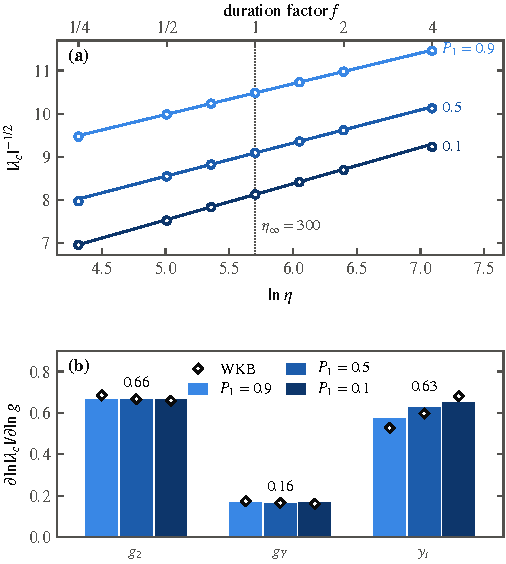
\includegraphics[width=0.7\textwidth]{prd_universality}
\caption{Universality of the finite-volume threshold.
(a)~$|\lamc|^{-1/2}$ grows linearly with the logarithm of the conformal duration $\eta=f\eta_\infty$ for $\Pone=0.9$, $0.5$, and $0.1$ (circles: hazard thresholds; lines: Eq.~(\ref{eq:rb-eta}) from $f=1$).
(b)~Logarithmic derivatives of $|\lamc|$ with respect to $g_2$, $g_Y$, and $y_t$ at $\mub$ (bars) and their WKB estimates (diamonds): the threshold is set mainly by $g_2$ and $y_t$, nearly independently of $\Pone$.} %
\label{fig:rb-universality}
\end{figure}

\subsection{Other spin structures}
\label{sec:rb-spin}

Tori with one or two periodic edges (spin structures PPA and PAA) also turn around once the holonomy sits at its one-loop vacuum.
On a periodic edge the fermions no longer pin the holonomy: at trivial holonomy the hypercharge curvature on that edge is $\kappa_Y=-1.675$ (PPA) and $-1.029$ (PAA), against $+0.700$ for AAA. %
Scanning the hypercharge, SU(2) Cartan, and SU(3) center holonomies edge by edge, we find that the one-loop vacuum on each periodic edge is an SU(3) center element, under which the quarks are twisted by $\pm\frac13$ and the Higgs, $W$, $B$, and gluons are not twisted; it lies $7.89/L$ (PPA) and $4.69/L$ (PAA) below the trivial holonomy per edge. %
This raises the Casimir weight to $\NC=21.07$ (PPA) and $23.67$ (PAA), compared with $25.52$ for AAA, and the shape has a tetragonal stationary point, at which $\NC=19.72$ and $22.84$; as for the AAA cube, the energy is a maximum along the aspect directions. %
The backgrounds differ little: $\Lb\MPbar=655$ and $693$, $\eta_\infty=331$ and $312$, and $\mub=3.72\times10^{15}$ and $3.51\times10^{15}\GeV$, which by themselves move $m_c$ by $-0.03$ and $-0.01\GeV$. %

The Higgs zero mode exists in both cases, because the Higgs is not twisted, and there are no fermion zero modes, because Grassmann constant modes require three periodic edges.
Two ingredients of the zero-mode model change.
The top-quark tadpole, $\propto Z_1(\vartheta_{\rm top})$, is $0.851$ (PPA) and $0.933$ (PAA) times its AAA value. %
The hypercharge curvature on the periodic edges stays negative at the center vacuum, $\kappa_Y=-0.556$ and $-0.304$, so the $\bm w$ direction is inverted, $\Omega_{\rm eff}^2(r)+\Omega_{X,i}^2<0$, for $r<1.5$ (PPA) and $r<1.1$ (PAA), across the well of the resonance. %
Our isotropic $(r,|\bm w|)$ model with a quadratic $\Omega_X^2$ does not apply there; it would need the exact twist energy along the periodic edges, an anisotropic $\bm w$, and the top matching at center holonomy.
An indicative estimate, which scales the cross terms with the direction-averaged curvatures and adds the changes of the background and of the top-quark tadpole, gives $\Delta m_c\approx+0.08$ and $+0.02\GeV$ relative to AAA, or $|\Delta\lamc|\lesssim0.0013$: the magnitude of $\lamc$ is unchanged, and its exact value depends on the sector and needs an anisotropic model. %
At trivial holonomy the fully periodic torus has $\NC=-30$ and does not turn around; with an SU(3) center holonomy its weight is positive, $\NC=11.2$, but the cusps of the lepton zero modes destabilize the electroweak holonomy, and we do not analyze this sector. %

\subsection{Sectors with 't~Hooft flux}
\label{sec:rb-flux}

Requiring all Standard Model fields to be single valued in a twisted sector, the $Z_6$ structure of the Standard Model allows a non-trivial SU(3) or SU(2) twist only together with a hypercharge flux, and the minimal flux is $|\Phi_Y|=2\pi$, reached for $(k_3,k_2)=(\pm1,1)$; a twist in SU(3) alone needs $4\pi$, and in SU(2) alone $6\pi$. %
The classical energy of the flux is
\begin{equation}
E_{\rm flux}=\frac{\Phi_Y^2}{2g_Y^2L}\ge\frac{2\pi^2}{g_Y^2L}=\frac{100.7}{L}, %
\label{eq:rb-flux}
\end{equation}
which is $2.36$ times the entire AAA Casimir energy; a turn would need $\NC>60$, whereas the Standard Model content gives at most $25.5$ in any flat twist, so these sectors cannot turn around. %
In them the Higgs doublet has no constant mode; its lowest mode is a Landau level with $\omega_0=\sqrt\pi/L$, and Landau levels replace zero-point confinement.
The corresponding threshold is $\lamc\approx-1$ ($-0.97$, $-1.36$, and $-1.84$ at $\Pone=0.9$, $0.5$, and $0.1$, uncertain by a factor of about $1.5$ through the Abrikosov parameter), two orders of magnitude more negative than for AAA, but irrelevant for the criterion because these sectors host no turn. %
The threshold of about $-0.01$ is therefore not an accident of the discrete choice AAA, while its precise value, to $10$--$20\%$, depends on the sector and on the Standard Model inputs. %

\subsection{The curvature coupling: zero-mode condition}
\label{sec:rb-xic}

The survival probability $\Pone$ applies when the late turn does not destroy the zero mode, which sets a lower bound on the Higgs curvature coupling $\xiH$.
Under assumption (A6), $\xiH$ is defined at $\mub$ as the coefficient of $R\,\Phi^\dagger\Phi$ in the zero-mode Hamiltonian; it is required by renormalization in curved spacetime~\cite{Birrell:1982ix}, so this is a condition on a Standard Model parameter.
For $\xiH<1/6$ the inverted oscillator of Eq.~(\ref{eq:rb-conformal}) acts, and we follow it with the lens transformation and the quantum--classical switch of Sec.~\ref{sec:rb-late}.
We define the threshold by
\begin{equation}
P_{\rm surv}(\xic)=0.99\,P_{\rm surv}(\tfrac16), %
\label{eq:rb-xic}
\end{equation}
with $P_{\rm surv}$ from the real-time evolution; for $\xiH\ge\xic$ the survival probability is $\Pone$ to $1\%$.
The main uncertainty is the late-time running prescription of $\lambda$ (Sec.~\ref{sec:rb-late}), and we quote the midpoint and half-difference.

\begin{table}[t]
\centering
\caption{Zero-mode threshold $\xic$ on $\xiH(\mub)$ in the final model, with the half difference of the two running prescriptions, the range over all prescription and switching variants, and the electroweak-scale image $\xi_{\rm EW}$.} %
\label{tab:rb-xic}
\begin{tabular}{ccccc}
\toprule
$m_t$ [GeV] & $\Pone$ & $\xic(\mub)$ & Range & $\xi_{\rm EW}$ \\
\midrule
$172.2$ & $0.985$ & $0.0346(40)$ & $0.030$--$0.039$ & $0.0525$ \\ %
$172.6$ & $0.843$ & $0.0737(25)$ & $0.071$--$0.077$ & $0.0862$ \\ %
$172.95$ & $0.511$ & $0.1195(6)$ & $0.119$--$0.121$ & $0.1258$ \\ %
$172.96$ & $0.499$ & $0.1206(7)$ & $0.120$--$0.121$ & $0.1267$ \\ %
$173.0$ & $0.455$ & $0.1248(5)$ & $0.124$--$0.126$ & $0.1304$ \\ %
\bottomrule
\end{tabular}
\end{table}

Table~\ref{tab:rb-xic} gives the threshold in the final model. %
We obtained it by repeating the whole real-time chain with the final cross terms: $145$ node potentials, a calibration that converged to $|\Delta\ln\Gamma|\le6\times10^{-8}$ with $A=0.0124$--$0.0144$, and $55$ real-time evolutions; with the earlier cross terms the same chain reproduces the earlier node potentials exactly. %
At the measured top mass the survival probability stays within $1\%$ of its conformal value for $\xiH(\mub)\gtrsim\xiHcentral$, or $\gtrsim\xiHmin$ including all prescription variants, and at the $\Pone=1/2$ point, $m_t=172.9595\GeV$, interpolation gives $\xic=0.1205(7)$, that is $\xiH\gtrsim\xiHhalf$. %
Below the threshold the survival probability decreases gradually: at $m_t=172.6\GeV$ it falls by $3.5$--$5\%$ at $\xiH=0.04$ and by $13$--$19\%$ at $\xiH=0.02$, and only for $\xiH\to0$ does the zero mode run away (Sec.~\ref{sec:rb-late}). %
The two-dimensional real-time evolution agrees with the calibrated one-dimensional model to $2\times10^{-4}$ in $P_{\rm surv}$ and to $1.4\times10^{-4}$ in $\xic$. %

\paragraph{Universality of $\xic(\Pone)$.}
The threshold is close to a universal function of $\Pone$.
Two versions of the model and the 11 of the 16 variants of the Standard Model inputs and $\alpha_s$ whose $\Pone$ lies in the tested range $0.45\lesssim\Pone\lesssim0.998$ lie on one curve $\xic(\Pone)$ to within $0.002$, and the final model lies on it to $0.0002$ [Fig.~\ref{fig:rb-hazard}(c)]. %
At fixed $m_t$ the final corrections lower $\xic$ by $0.0004$, because they raise $\Pone$. %
Stated through $\Pone$, or through $\lambda(\mub)$, the condition is therefore free of the Standard Model and $\alpha_s$ errors at first order.
At fixed $m_t=172.6\GeV$ these errors widen $\xic$ by $\pm\xiHbandSM$ and $\pm\xiHbandAs$, respectively. %
These bands were computed with the earlier model by shifting $\lambda$ by $\mp|d\lambda(\mub)/dm_t|\times0.10\GeV$ and by repeating the chain at $\alpha_s=0.1171$ and $0.1189$; through the universal curve they carry over to the final model with their midpoints lowered by about $0.0004$. %
In the earlier model they are $0.0750\pm0.0130$ and $0.0795\pm0.0397$ at $m_t=172.6\GeV$ (midpoint and half width). %
The two sides are asymmetric because $\xic$ saturates toward $1/6$ as $\Pone\to0.1$.
The scale of $\xiH$ adds a smaller ambiguity: the $\xiH$-dependent loss occurs at $\tau\approx3.5$--$6$, where $\mu\approx10^{13}$--$10^{14}\GeV$, and the running of $\xi$ between there and $\mub$ is estimated at $0.0005$--$0.002$. %

\paragraph{Running to the electroweak scale.}
The coupling runs as~\cite{Herranen:2014cua,Mantziris:2020rzh}
\begin{equation}
\xi(\mu)=\tfrac16+\bigl(\xi_{\rm EW}-\tfrac16\bigr)\Xi(\mu),\qquad
16\pi^2\frac{d\ln\Xi}{d\ln\mu}=12\lambda+6y_t^2-\tfrac32g_Y^2-\tfrac92g_2^2,
\label{eq:rb-xirun}
\end{equation}
with $\Xi(\mub)=1.155$, so that $\xiH(\mub)=\xiHmin$ corresponds to $\xi_{\rm EW}\approx\xiHminEW$ at $\mu=m_t$; the conformal value $1/6$ is a fixed point of the one-loop running. %

\subsection{The curvature coupling: all-mode bound during inflation}
\label{sec:rb-xiinf}

After the turn the plateau inflates, and long-wavelength Higgs fluctuations can nucleate the true vacuum~\cite{Espinosa:2007qp,Hook:2014uia,Kearney:2015vba,Espinosa:2015qea,Joti:2017fwe,Markkanen:2018pdo}.
The plateau of assumption (A3) is a minimally coupled scalar with a Starobinsky-shaped potential and no $R^2$ term, so the field-theory criterion of Ref.~\cite{Mantziris:2020rzh} applies, and the $R^2$ bound $\xi_{\rm EW}\gtrsim0.1$ of Ref.~\cite{Mantziris:2022fuu} does not. %
We use the one-loop curved-space effective potential of Ref.~\cite{Markkanen:2018bfx} with renormalization-group improvement,
\begin{equation}
V_{\rm RGI}=\tfrac12\xi(\mu_*)Rh^2+\tfrac14\lambda(\mu_*)h^4+\frac{\alpha(\mu_*)}{144}R^2,
\label{eq:rb-VRGI}
\end{equation}
where $h$ is here the Higgs field, $\mu_*$ the field- and curvature-dependent renormalization scale, and $\alpha$ the coefficient of $R^2$ generated by the running, together with the Hawking--Moss rate~\cite{Hawking:1981fz}
\begin{equation}
\Gamma_{\rm HM}=\Bigl(\frac{R}{12}\Bigr)^2e^{-B},\qquad B=\frac{384\pi^2\Delta V}{R^2},
\label{eq:rb-HM}
\end{equation}
with $\Delta V$ the height of the barrier of $V_{\rm RGI}$.
We require less than one bubble in the past light cone, $\langle N\rangle=\int\gamma(N)\,dN<1$, where
\begin{equation}
\gamma(N)=\frac{4\pi}{3}\Bigl[a_{\rm inf}\Bigl(\frac{3.21\,e^{-N}}{H_0}-\tilde\eta\Bigr)\Bigr]^3\frac{\Gamma_{\rm HM}}{H},\qquad \frac{d\tilde\eta}{dN}=-\tilde\eta-\frac{1}{a_{\rm inf}H},\quad\tilde\eta(0)=0,
\label{eq:rb-lightcone}
\end{equation}
counts the bubbles per $e$-fold $N$ of inflation in the past light cone of today's observer, following Refs.~\cite{Mantziris:2020rzh,Mantziris:2022fuu}, with the background integrated without the slow-roll approximation. %
The end of inflation is $\dot H/H^2=-\frac14$; taking $\ddot a=0$ instead changes the bound by less than $10^{-4}$, and the start of the integration at the turn ($N=68.47$) does not matter, because the integral is dominated by the last $e$-folds. %
On the torus the past light cone is cut by the cube of edge $6/H_0$, which keeps $98.1\%$ of its volume ($\Delta B=0.019$), a negligible change. %
This implementation reproduces $\xi_{\rm EW}=0.05946$ of Ref.~\cite{Mantziris:2020rzh} (target $0.05938$). %

For $m_t=172.2$, $172.6$, and $173.0\GeV$ we find $\xi_{\rm inf}(\mub)=0.030$, $0.038$, and $0.044$, or $\xi_{\rm EW}=0.049$, $0.055$, and $0.060$. %
At the same scale the zero-mode threshold and the inflationary bound coincide at $\lambda(\mub)\approx-0.0065$, i.e., $m_t\approx172.1\GeV$, and the zero-mode condition is the stronger one above this mass (Fig.~\ref{fig:rb-xi}). %
The two calculations cover adjacent epochs: the zero-mode calculation until the torus leaves the Hubble radius about five $e$-folds after the turn, and the light-cone count afterward; the transition contributes at most $O(10)\,e^{-B}$ with $B\gtrsim180$ to $\langle N\rangle$, but we have not simulated it jointly. %

After inflation the plateau oscillates with $H_{\rm end}\approx7\times10^{12}\GeV$, far above the instability scale, so the analysis of Ref.~\cite{Herranen:2015ima} applies: $\xi\lesssim1$ avoids destabilization by curvature oscillations, and $\xi<3/8$ avoids tachyonic resonance. %
The allowed window is
\begin{equation}
\max(\xic,\xi_{\rm inf})\le\xiH\lesssim1,
\label{eq:rb-window}
\end{equation}
and the conformal value $\xiH=1/6$ lies inside it in both scale readings.

\begin{figure}[t]
\centering
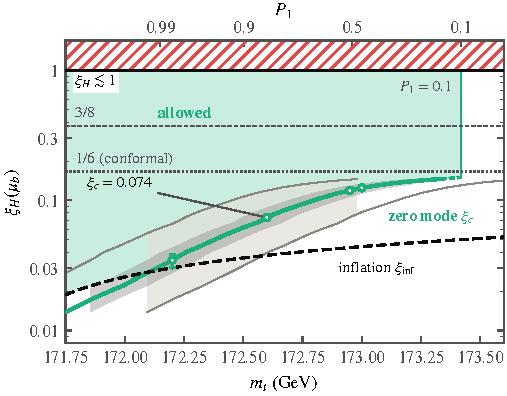
\includegraphics[width=0.6\textwidth]{prl_fig3_xi}
\caption{Curvature coupling needed for survival.
The zero-mode threshold $\xic(\mub)$ (solid; circles: direct calculations; dark and light bands: Standard Model mapping and $\alpha_s$) and the all-mode bound $\xi_{\rm inf}$ from plateau inflation (dashed) bound $\xiH$ from below, and $\xiH\lesssim1$~\cite{Herranen:2015ima} bounds it from above (hatched).
Survival with $\Pone\geq0.1$ requires $\xiH$ in the shaded region; the dashed end of the line extrapolates below $\Pone=0.13$.
Dotted: the conformal value $1/6$; thin dashed: $\xi=3/8$.
The zero-mode condition is the stronger one for $m_t\gtrsim172.1\GeV$.} %
\label{fig:rb-xi}
\end{figure}

\section{The emptiness gate}\label{rep:gate}

At the turning point the light fields can carry only the energy that the Casimir energy leaves free, and we show that this is very little.
The whole negative energy of the torus is worth about five quanta of its lowest nonzero bosonic modes. %
A reheating coupling in a time-symmetric past exceeds this budget by more than $10^{94}$, and natural states of the non-conformal fields must be prepared within about seven e-folds of the turning point. %
We therefore read the turning point as a beginning.
The budget limits the excitation of the light fields but does not select their vacuum: zero-mode excitations and a single photon pair fit inside it, and the photon pair turns the universe around and freezes the torus into an elongated box.
The chapter derives the budget (Sec.~\ref{rA:g-budget}), evaluates the two channels that every realistic history contains (Secs.~\ref{rA:g-reheating} and~\ref{rA:g-preparation}), states the reading that follows (Sec.~\ref{rA:g-beginning}) and computes the excitations that the budget allows (Sec.~\ref{rA:g-excited}).

\subsection{An exact budget}
\label{rA:g-budget}

At a turning point, $H=0$, the Friedmann constraint of Eq.~\eqref{eq:rA-einstein} reads
\begin{equation}
\rho_\phi+\rho_C+\rho_{\rm exc}+\tfrac12\MPbar^2S=0,
\label{eq:rA-g-constraint}
\end{equation}
where $\rho_\phi$ is the inflaton energy density, $\rho_{\rm exc}\geq0$ is the energy of the light fields above their ground state and $\rho_C$ is the ground-state (Casimir) energy, zero modes included.
Every term except $\rho_C$ is non-negative, and $\rho_\phi\geq V>0$ is strictly positive.
Multiplying by $L^3$, the total excitation energy therefore obeys
\begin{equation}
E_{\rm exc}<|E_C|=\frac{\rANeff\rAgam}{\Lb},\qquad \rANeff=(1-\fzm)\NC
\end{equation}
(Secs.~\ref{rep:casimir}--\ref{rep:zeromodes}).
For free massless quanta at the cube the frequencies are $2\pi|\bm n-\bm\vartheta|/L$, with $\bm\vartheta$ the twist of the field, and $|\bm n-\bm\vartheta|\geq\sqrt3/2$ for AAA fermions.
Summing over the excited quanta, $E_{\rm exc}=(2\pi/L)\sum_{\rm quanta}|\bm n_i-\bm\vartheta_i|$, and the budget becomes
\begin{equation}
\sum_{\rm quanta}|\bm n_i-\bm\vartheta_i|<\frac{\rANeff\rAgam}{2\pi}=0.2666\,\rANeff .
\label{eq:rA-emptiness}
\end{equation} %
The entire negative energy of a cubic torus is thus worth $0.27$ lowest-mode quanta per unit of $\rANeff$. %
For the Standard Model with the zero-mode share $\fzm=0.30$ the right side is $0.2666\times17.86=4.76$: %
at the turning point the whole universe can hold about five quanta of its lowest nonzero bosonic modes, or $4.76/(\sqrt3/2)=5.5$ of its lowest fermionic modes, all fields together. %
Across the allowed range of the zero-mode share, $0.258\leq\fzm\leq0.308$ (Sec.~\ref{rep:zeromodes}), the bosonic bound runs from $4.7$ to $5.05$; it is $4.90$ at the next-order value $\fzm\simeq0.28$ and $6.80$ for free fields. %
Table~\ref{tab:rA-budget} lists the bound across the range, from the Gaussian variational bound $\fzm=0.308$ to the pure-gauge bound $0.258$, with $\NC=25.515$ for the AAA Standard Model plus the static graviton, together with the number of lowest AAA fermion quanta, with $|\bm n-\bm\vartheta|=\sqrt3/2$, that the same budget holds. %
The bosonic bound equals 5 at $\fzm=0.265$; it lies below 5 at the leading and next-order values and slightly above 5 at the lower end of the range, which is why we quote about five quanta. %
A single quantum with $|\bm n|\gtrsim5$ already forbids the turn when $\fzm>0.265$, and a single quantum with $|\bm n|\geq\sqrt{26}$, for example $\bm n=(5,1,0)$, forbids it for every $\fzm>0.250$. %
Excitations of the zero modes are cheaper; we return to them in Sec.~\ref{rA:g-excited}.

\begin{table}[tbp]
\centering
\caption{The emptiness budget across the zero-mode share $\fzm$: the bound on $\sum|\bm n-\bm\vartheta|$ of Eq.~\eqref{eq:rA-emptiness}, the equivalent number of lowest AAA fermion quanta, the shift of $\log_{10}R$ of Eq.~\eqref{eq:rA-windowR} caused by the zero-mode energy, and the preparation time $T$ (in e-folds before the turn) at which three non-conformal degrees of freedom exhaust the budget for $h\Lb=0.0044$.}
\label{tab:rA-budget}
\begin{tabular}{lccccc}
\toprule
$\fzm$ & 0.308 & 0.30 & 0.28 & 0.258 & 0\\ %
\midrule
bosonic bound & 4.705 & 4.762 & 4.898 & 5.047 & 6.802\\ %
fermion quanta & 5.43 & 5.50 & 5.66 & 5.83 & 7.85\\ %
$\Delta\log_{10}R$ & --- & 0.155 & 0.143 & 0.130 & 0\\ %
$T$ & --- & 6.909 & 6.913 & 6.918 & 6.960\\ %
\bottomrule
\end{tabular}
\end{table}

\paragraph{Thermal states.}
For the Maxwell toy a thermal state satisfies Eq.~\eqref{eq:rA-emptiness} only if $L\Theta<1.45$ (exact lattice sums), a temperature at which each field holds $0.23$ thermal quanta on average; the AAA Standard Model allows a lower temperature still, because its antiperiodic fermions carry thermal energy but little Casimir weight. %

\paragraph{Earlier semiclassical forms.}
Excitations weaken the support of a Casimir turning point, and this has been seen before in semiclassical form.
In a fluid model of a flat torus a bounce needs a negative total density of radiation-like matter~\cite{Godlowski:2007gx}.
In the minisuperspace model of Mithani and Vilenkin, excited radiation lowers the Casimir coefficient to $C_{\rm eff}=C-C_r$~\cite{Mithani:2014toa}, where $C_r$ is the coefficient of a radiation term that can be tuned; they note that it becomes discrete once the conformal fields are quantized on the compact space.
Equation~\eqref{eq:rA-emptiness} is the quantized form of that statement.
It bounds the occupation numbers of the field modes, weighted by their wave numbers, by $\rANeff\rAgam/2\pi\simeq\rANeff/4$, which is a handful of quanta for the Standard Model.

\paragraph{What can violate the budget.}
Radiation and Casimir energy both dilute as $L^{-4}$.
For conformal fields isotropic expansion does not create quanta~\cite{Parker:1969au}, so the occupation numbers are constant, every quantum redshifts as $1/L$, and the left side of Eq.~\eqref{eq:rA-emptiness} is conserved by the adiabatic evolution of conformal fields.
The budget can therefore be violated only by non-conformal fields, by couplings that break conformal invariance, or by the state itself.
For the same reason a phase of ultra-stiff contraction, which dilutes shear relative to radiation, leaves the ratio of radiation to Casimir energy unchanged, and dissipation into radiation only raises it; neither can empty the torus.
We now evaluate the two channels that any realistic history contains.

\subsection{A reheating coupling in a time-symmetric past}
\label{rA:g-reheating}

The plateau history is time symmetric about the turning point (Sec.~\ref{rep:turning}).
Its remote contracting branch is the time reverse of reheating, with the inflaton oscillating about the minimum of $V$, so any coupling that reheats the universe after inflation also acts there.

\paragraph{The coupling.}
We take the visible coupling $-I^2(\phi)F_{\mu\nu}F^{\mu\nu}/4$ with
\begin{equation}
I^2=1+c_v\,\frac{\phi}{\MPbar}\,f(|\phi|),\qquad c_v=0.01 . %
\end{equation}
The window $f$ is smooth, equals 1 for $|\phi|\leq0.5\MPbar$ and 0 for $|\phi|\geq1.5\MPbar$, and leaves the turning point exactly conformal. %
The coupling reheats the universe through the perturbative width $\Gamma_\phi=12c_v^2m_\phi^3/(64\pi\MPbar^2)$~\cite{Garcia:2023obw}, which gives the weak-decay history of Sec.~\ref{rep:spectra}.

\paragraph{Mode equations.}
We write the free photon mode as $A_{\bm k}$, with action $\tfrac12\int d\eta\,I^2(A'^2-k^2A^2)$ and canonical momentum $\Pi_A=I^2A'$.
The mode equation is $(I^2A')'+k^2I^2A=0$; outside the window, where $I=1$, Maxwell theory is conformal and $A$ oscillates with constant occupation.
The background is the time-symmetric plateau history calibrated by the weak decay, with $\phi_b=5.475227\,\MPbar$ and $h/\MPbar=6.7467\times10^{-6}$. %
We evolved the free photon modes on the contracting branch, declared the instantaneous vacuum at the $j$th extremum of the inflaton oscillation before its final climb onto the plateau ($j$ half-oscillations), and read out the exact occupation after the window closes.
At a contracting turning point of $\phi$, where $\dot I=0$, the instantaneous vacuum is
\begin{equation}
A=\frac{1}{I\sqrt{2k}},\qquad \Pi_A=-ikI^2A,
\end{equation}
and after the window closes the occupation is
\begin{equation}
n_k=\frac{|\Pi_A|^2/I^2+k^2I^2|A|^2}{2k}-\frac12 .
\end{equation}

\paragraph{The energy ratio.}
After the window photons and Casimir energy scale alike, as $L^{-4}$, and we compare them at the turning point.
Twelve vector fields with two polarizations each carry the energy density $\rho_\gamma=(12/\pi^2)\int k^4n_k\,d\ln k/a^4$, with $k$ comoving.
With $q=k/(a_{\rm end}h)$ and $n_{\rm end}=\ln(a_{\rm end}/a_b)$ the number of e-folds from the turning point to the end of inflation, $\rho_\gamma(a_b)=(12/\pi^2)h^4e^{4n_{\rm end}}\int q^4n_q\,d\ln q$.
At the turn the constraint gives $|\rho_C|=(1-\fzm)V(\phi_b)$ for the background calibrated with free fields, with $V(\phi_b)=v_b\MPbar^2h^2$.
The ratio is therefore
\begin{equation}
R=\frac{\rho_\gamma}{|\rho_C|}=\frac{12}{\pi^2}\Big(\frac h\MPbar\Big)^2\frac{e^{4n_{\rm end}}}{(1-\fzm)\,v_b}\int q^4n_q\,d\ln q,
\label{eq:rA-Rformula}
\end{equation}
with $v_b=V(\phi_b)/\MPbar^2h^2$ and prefactor $10^{97.79}$ at $\fzm=0$. %

\paragraph{Results.}
We used 97 log-spaced $q\in[10^{-3},100]$ at $j=1$, 2, 5, 10, 20, 40 and 85, and 401 log-spaced $q\in[10^{-3},30]$ at $j=1$ and 85 as a check, with relative tolerance $10^{-12}$ and Wronskian errors below $4\times10^{-10}$. %
With the free Casimir energy, $\log_{10}R=93.86$ at $j=1$ ($93.89$ with 401 wave numbers) and $96.28$ ($96.32$) at $j=85$. %
The zero-mode energy lowers $|\rho_C|$ and raises the exponent by $\log_{10}[1/(1-\fzm)]=0.155$ at $\fzm=0.30$, which gives
\begin{equation}
R=\frac{\rho_\gamma}{|\rho_C|}=10^{94.0}\ (j=1),\ \ldots,\ 10^{96.5}\ (j=85)
\label{eq:rA-windowR}
\end{equation} %
[Fig.~\ref{fig:rA-gate}(a)].
Across the allowed range of $\fzm$ the exponent changes by at most $0.03$ (Table~\ref{tab:rA-budget}). %
Using $\rAHeff$ instead of $h$ changes the exponent by $-0.009$, the instant-reheating calibration $h/\MPbar=6.116\times10^{-6}$ by $-0.085$, and a present size $L_0=2\,\dLSS$ instead of $0.95\,\dLSS$ by $+1.29$, since $R\propto e^{4n_{\rm end}}$ and the longer plateau adds to $n_{\rm end}$. %
The origin of the excess is simple: when the window closes the Casimir energy is $3.5\times10^{-107}$ of the scalar energy, so a production efficiency of $10^{-13}$ outweighs it by more than ninety orders of magnitude. %

\paragraph{Independent check.}
Time reversal maps this problem onto the expanding-branch emission from a vacuum set just after the window opens.
An independent code for that problem agrees mode by mode, to $5\times10^{-8}$ for $q\leq1$, $10^{-6}$ at $q=3$ and $3\times10^{-3}$ at $q=10$, where $n_q<3\times10^{-9}$, and its band integral at $j=85$ agrees to $0.5\%$. %

\paragraph{Consequence.}
For perturbative couplings the produced energy scales as $c_v^2$, so a coupling weak enough to give $R<1$ would be far too weak to reheat.
A time-symmetric history with a reheating coupling therefore cannot be continued into its own past, unless the photon state before the window is the backward evolution of the post-window vacuum, a correlated state that carries more than $10^{94}$ times the Casimir energy until the window removes it. %

\begin{figure}[tbp]
\centering
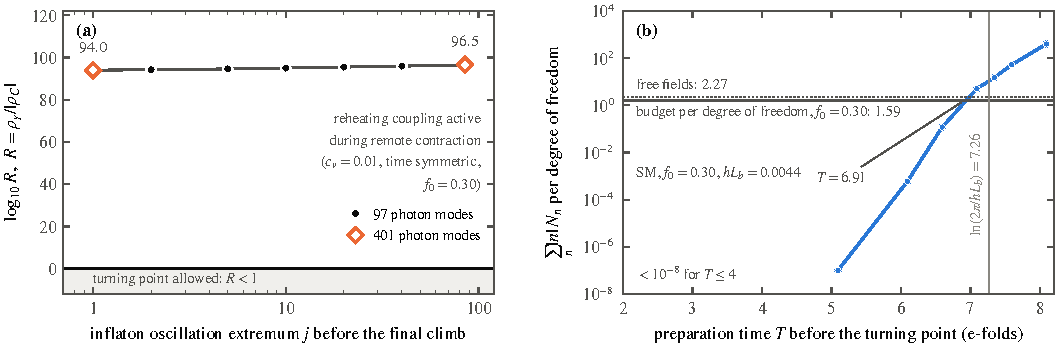
\includegraphics[width=\textwidth]{prd_emptiness_gate}
\caption{Energy at the turning point against the Casimir budget. (a)~Ratio $R$ of the comoving energy of visible photons from a reheating coupling ($c_v=0.01$) in the remote contraction of the time-symmetric history to the comoving Casimir energy with its zero-mode part, for photon vacua declared at the $j$th inflaton extremum; the turn needs $R<1$. (b)~Excitation $\sum_{\bm n}|\bm n|N_{\bm n}$ per non-conformal degree of freedom of a natural state declared $T$ e-folds before the turn; horizontal lines: one third of the budget~\eqref{eq:rA-emptiness}, at $\fzm=0.30$ (solid) and for free fields (dotted); vertical line: $T=\ln(2\pi/h\Lb)$.} %
\label{fig:rA-gate}
\end{figure}

\subsection{Non-conformal fields and the latest preparation}
\label{rA:g-preparation}

\paragraph{Mode equation.}
Gravitons, any minimally coupled massless scalar and, up to slow-roll corrections, the inflaton fluctuation obey $v''+(k^2-a''/a)v=0$ for $v=a\chi$ in conformal time.
On the turning-point solution, Eq.~\eqref{eq:rA-turning-solution}, $a''/a=2h^2a^2$ exactly, as in de~Sitter space, because the Casimir stress is traceless (Eq.~\eqref{eq:rA-app}).
In cosmic time the same equation reads
\begin{equation}
\ddot v+H\dot v+\Big(\frac{k^2}{a^2}-2h^2\Big)v=0 .
\label{eq:rA-g-modeeq}
\end{equation}

\paragraph{Horizon exit before the turn.}
Every torus mode is deep inside the Hubble radius at the turning point, $k/(a_bh)=2\pi|\bm n|/(h\Lb)\gtrsim1400$ (1300 for free fields), where the adiabatic vacuum is unambiguous. %
Going back in time, mode $\bm n$ leaves the Hubble radius when $a=2\pi|\bm n|/h$, that is $\ln(2\pi|\bm n|/h\Lb)$ e-folds before the turning point.
A state declared $T$ e-folds before the turning point can be adiabatic (Hadamard) only for the modes inside the Hubble radius at that time.
Modes outside it have no adiabatic vacuum, and natural choices, such as the instantaneous ground state of the field or the conformal vacuum, leave them excited when they re-enter.

\paragraph{Computation.}
At $t_i$, with $a(t_i)=a_be^T$, modes with $k>1.5\,a_ih$ receive the second-order adiabatic vacuum. %
Modes with $k<a_ih$ receive either the instantaneous ground state of $\chi$ or the conformal vacuum, two choices that differ by at most $0.001$ e-fold in the crossing and are indistinguishable in Fig.~\ref{fig:rA-gate}(b), and modes with $a_ih\leq k\leq1.5\,a_ih$ receive the conformal vacuum. %
We integrate Eq.~\eqref{eq:rA-g-modeeq} to the turn and read the occupation $N_{\bm n}$ relative to the adiabatic vacuum at $t=0$; the lattice sum over $\bm n$ uses interpolation in $\ln|\bm n|$.
Because $a''/a=2h^2a^2$ holds exactly, the only parameters of the problem are $T$ and $k/(a_bh)=2\pi|\bm n|/h\Lb$, and a change of $h\Lb$ is a change of the e-fold at which each mode exits.
The occupations therefore obey the scaling $N_{\bm n}(T,h\Lb)=N_{\bm n}(T+\ln[h\Lb/(h\Lb)_0],(h\Lb)_0)$, which a direct recomputation of two modes confirms to $3.5\times10^{-9}$. %
The crossings of Table~\ref{tab:rA-budget} follow from the Standard Model occupations by this scaling; for $h\Lb=0.0048$ each is lower by $\ln(0.0048/0.0044)=0.087$. %

\paragraph{Results.}
Figure~\ref{fig:rA-gate}(b) shows the result.
The excitation per degree of freedom is below $10^{-8}$ of a quantum for $T\leq4$. %
With three non-conformal degrees of freedom it exhausts the budget at $T=6.91$ for the Standard Model with $\fzm=0.30$ and $h\Lb=0.0044$, and at $6.96$ for free fields; beyond that it grows roughly as $e^{4T}$. %
The count takes the Higgs doublet to be conformally coupled; for $\xiH(\mub)\simeq0.08$ its four components are partly non-conformal, and even if they were excited like minimally coupled scalars, the $e^{4T}$ growth would move the crossing closer to the turn by only $\ln(7/3)/4\simeq0.2$ e-fold. %
The two choices for modes outside the Hubble radius change this crossing by at most $0.001$, and the $30\%$ smaller budget left by the zero modes moves it by only $-0.05$ e-fold. %
A natural state must therefore be prepared within $6.9$ e-folds of the turning point ($6.82$ for $h\Lb=0.0048$), shortly after the whole torus has entered the Hubble radius at %
\begin{equation}
T_{\max}\simeq\ln\frac{2\pi}{h\Lb}=7.26
\label{eq:rA-Tmax}
\end{equation} %
e-folds before the turn ($7.18$ for $h\Lb=0.0048$). %
If the state is instead set in the remote matter-dominated contraction, modes leave the horizon and grow there~\cite{Wands:1998yp,Finelli:2001sr}.
By time reversal their occupation at the turning point equals that of an inflationary mode long after it re-enters, which is enormous.

\subsection{A prepared beginning}
\label{rA:g-beginning}

The emptiness gate leaves two readings of a Casimir turning point.
Either the contracting branch is a genuine past, which requires a state arranged over the whole infinite contraction so that it evolves into the turning-point vacuum, squeezed in every non-conformal mode and correlated against every coupling.
Or the state is specified at the turning point, or within about seven e-folds of it.
Both readings describe the same quantum state; they differ in where that state is specified.
Specifying it in the remote past requires the correlations just described, while specifying it at the turn requires only the vacuum of the light fields, so we adopt the second (assumption~\ref{assump:A4}).

A time-symmetric state then makes the turning point a minimum of the coarse-grained entropy of the light fields,
\begin{equation}
\mathcal S_{\rm cg}=\sum_{\bm k}\big[(n_{\bm k}+1)\ln(n_{\bm k}+1)-n_{\bm k}\ln n_{\bm k}\big],
\end{equation}
with $n_{\bm k}$ the adiabatic occupations.
This entropy vanishes at the turn and grows in both time directions, as modes leave the Hubble radius and, later, as reheating proceeds.
The contracting branch of Eq.~\eqref{eq:rA-turning-solution} is then the time mirror of the prepared state.
Its observers see their own expansion, inflation and reheating, with an arrow of time pointing away from the turn, as in time-symmetric cosmologies with two arrows~\cite{Carroll:2004pn,Barbour:2014bga} and in past-eternal inflation, whose arrows point away from a null boundary surface~\cite{Aguirre:2001ks,Aguirre:2003ck}; here they point away from a regular turning point (Fig.~\ref{fig:rA-turning}).
We call this the two-branch reading: both branches are futures of the turning point.
The geometric completeness of the solution (Sec.~\ref{rA:turn-complete}) is then no eternal past.
The thermodynamic past of every observer ends at the turn, and the past-incompleteness theorem for expanding spacetimes~\cite{BordeGuthVilenkin2003} does not apply because $H$ averages to zero along every complete geodesic.
The low entropy at the turn is imposed, not explained.

In this reading the Casimir turning point is a beginning, at a torus $\Lb\simeq722\,\MPbar^{-1}$ across, a few thousand Planck lengths. %
This is in the spirit of toroidal quantum creation~\cite{Linde:2004nz,Godet:2026gqw}; in the creation scenario of Refs.~\cite{Zeldovich:1984vk,Guth:2025dal} the Lorentzian history starts at the turning point of the same solution.
For that case Guth and Vilenkin found that regularity confines the Bogoliubov coefficients of the field modes at nucleation to a narrow range near zero without fixing them, and concluded that creating a torus is either impossible or governed by Planck-scale physics~\cite{Guth:2025dal}.
The emptiness gate is a quantitative Lorentzian counterpart of that restriction.
Earlier treatments of the Casimir turning point discarded the contracting half by a duality argument~\cite{McInnes:2005sa}, took a classical contracting phase at face value~\cite{Godlowski:2007gx}, or assumed an empty torus without a turning point~\cite{Fornal:2026qfq}.

In what follows all light fields start in their adiabatic vacuum at the turning point, with the gauge zero modes in their ground state and the Higgs zero mode in its finite-volume resonance (Sec.~\ref{rep:h-survival}), and the shape moduli start in the natural state of assumption~\ref{assump:A8}; the gate allows this choice but does not enforce it.
The five shape moduli of the torus are collective coordinates of the geometry, and the gate constrains them far more strongly.
If their state is real at some instant, survival of the shape on both branches with probability $90\%$ requires, for a Gaussian state, that instant to lie within $0.35$ Hubble times of the turn (Sec.~\ref{rA:s-conditional}), a window $21$--$32$ times shorter in time than the one allowed for the light fields. %

\subsection{The gate does not select the vacuum}
\label{rA:g-excited}

The budget~\eqref{eq:rA-emptiness} limits the excitation, but it does not force the vacuum.

\paragraph{Zero-mode excitations.}
The cheapest neutral excitations are those of the zero modes.
The non-abelian levels lie $1.24/L$ ($SU(2)$) and $1.47/L$ ($SU(3)$) above the ground state~\cite{vanBaal:1988va,Pavel:2021mxn}, $3\%$ of the free Casimir coefficient $C$ each. %
The hypercharge mode, held at leading order only by the Higgs, is softer: a variational bound puts its first level at most $0.46/L$ up, $1\%$ of $C$. %
The budget, $(1-\fzm)C\simeq29.9$ in units of $1/L$, holds about twenty of the former and over sixty of the latter. %
By isospectrality (Proposition~\ref{prop:rA-isospectral}) they keep the cube stationary, but each raises the effective $\fzm$ by its share of $C$, and the fossil width $\sigma_E$ of Sec.~\ref{rA:s-fossil} by $8$--$9\%$ or by up to $3\%$, respectively. %

\paragraph{Pairs of nonzero modes.}
Among the nonzero modes, a pair of transverse hypercharge photons with opposite momenta along one edge is neutral, carries no momentum and costs $4\pi/L$, which is $29\%$ of the free Casimir energy and $42\%$ of what remains with the zero modes. %
A fermion--antifermion pair along a body diagonal, with momenta $\pm\sqrt3\,\pi/L$, costs $2\sqrt3\,\pi/L=10.88/L$, or $25\%$. %
Unlike the vacuum, such a pair drives the shape at linear order, because its energy $4\pi[(G^{-1})_{11}]^{1/2}/L$ depends on it.
A pair along one edge is a legitimate state but is not invariant under the cubic large diffeomorphisms.
A state invariant under them superposes the pairs along the three axes; the homogeneous stress has no matrix elements between pairs on different axes, so its mean is cubic and in semiclassical gravity it drives the shape only at second order.
The elongation computed below therefore belongs to a definite-axis state, or to one branch of the superposition if the branches decohere.

\paragraph{The photon-pair universe.}
On the torus a transverse hypercharge photon with comoving wave vector $\bm n$ has the frequency $2\pi(\bm n^{\mathsf T}G^{-1}\bm n)^{1/2}/L$.
A pair with $\bm n=(\pm1,0,0)$ therefore adds $4\pi[(G^{-1})_{11}]^{1/2}/L$ to the energy and lowers the Casimir coefficient to
\begin{equation}
C(G)=C_{\rm free}(G)-4\pi[(G^{-1})_{11}]^{1/2},
\end{equation}
with $C_b=C(\rAone)=42.74-12.57=30.174$ at the cube for free fields; a zero-mode energy $Q/L$ subtracts $Q$ from $C$. %
Maxwell theory is conformal, so the pair sees only the shape.
Its adiabaticity parameter $|d\Omega/d\eta|/\Omega^2$ peaks at $4.4\times10^{-4}$ for free fields and $1.8\times10^{-3}$ at $\fzm=0.30$, and the occupation stays fixed. %
The pair and the AAA twist leave the axis $X={\rm diag}(2,-1,-1)/\sqrt6$ invariant, so the shape can be restricted to $G=e^{2\beta X}$.
With $\tau=ht$, $\varrho=L/\Lb$, $\Lb^4=C_b/3\MPbar^2h^2$ and $u=H/h$, the minisuperspace action~\eqref{eq:rA-minisuperspace} with the energy $E=3\MPbar^2h^2L^3-C(\beta)/L$ gives the following equations.
The shear is $S=h^2v^2$ with $v=\beta'$, because $\sigma=\tfrac12G^{-1}\dot G=\dot\beta X$ and $\Tr X^2=1$.
The constraint $3\MPbar^2H^2=\rho+\tfrac12\MPbar^2S$ with $\rho=3\MPbar^2h^2-C/L^4$ and $1/(\MPbar^2h^2L^4)=3/(C_b\varrho^4)$ becomes
\begin{equation}
3u^2-3+\frac{3C}{C_b\varrho^4}-\frac{v^2}{2}=0 .
\label{eq:rA-pair-constraint}
\end{equation}
The radiation-like part has $\rho+\bar p=\tfrac43(-C/L^4)$, so $\dot H=\tfrac23C/(\MPbar^2L^4)-\tfrac12S$, and the shape equation $d(\MPbar^2L^3\dot\beta)/dt=C'(\beta)/L$ follows from Eq.~\eqref{eq:rA-minisuperspace}.
Altogether
\begin{equation}
\begin{aligned}
(\ln\varrho)'&=u,& u'&=\frac{2C}{C_b\varrho^4}-\frac{v^2}{2},\\
\beta'&=v,& v'&=-3uv+\frac{3C'(\beta)}{C_b\varrho^4}.
\end{aligned}
\label{eq:rA-pair-eqs}
\end{equation}
A turning point $u=0$ has $C(\beta_0)/(C_b\varrho_0^4)=1+v_0^2/6$ by Eq.~\eqref{eq:rA-pair-constraint}, that is $\varrho_0^4=C(\beta_0)/[C_b(1+v_0^2/6)]$, and the universe turns around because there $u'=2(1+v_0^2/6)-v_0^2/2=2-v_0^2/6>0$ for every shape velocity with $v_0^2<12$.

\paragraph{Results.}
We evolved the volume and the shape of a torus that is cubic and at rest at the turning point and holds one photon pair, whose occupation stays adiabatic.
Starting from the cube at rest, the free-field universe turns around, re-expands and the shape freezes at $\beta_\infty=0.4511$, with sides in the ratio $e^{\sqrt{3/2}\,\beta_\infty}=1.738$, since $G=e^{2\beta X}$ gives $L_1/L_2=e^{(2/\sqrt6+1/\sqrt6)\beta}$. %
Two independent evaluations of the twisted sums and several integrator settings give $\beta_\infty$ to $3\times10^{-13}$, and the constraint holds to $2\times10^{-11}$. %
Starting deformations of $\pm0.0066$ and $\pm0.02$ and initial shape velocities of $\pm0.02$ give ratios between $1.41$ and $2.10$, and their combinations between $1.34$ and $2.20$. %
An evolution of all five shape moduli from small deformations shows the second aspect direction growing by a factor $14.3$ and the angles oscillating and decaying to about a third; all runs freeze. %
At $\fzm=0.30$, $C_b=17.36$ and the sides freeze in the ratio $4.96$; for $\fzm=0.258$, $0.286$, $0.308$ and $0.32$ the ratio is $3.56$, $4.35$, $5.43$ and $6.31$. %
A second implementation, with its own integrator and a spline of the twisted Ewald sums, reproduces $\beta_\infty$ at $\fzm=0$ and at $Q=0.246\,C_{\rm free}$ (ratio $3.31$) to $10^{-8}$. %
The universe therefore turns around, expands and freezes into an elongated box with sides in the ratio $1.74$ for free fields and $4.96$ at $\fzm=0.30$, or $3.6$--$5.4$ across the allowed range of $\fzm$. %

\paragraph{Quantum spread of the branch.}
These ratios are branch centers for a shape that is exactly cubic and at rest at the turn.
An independent evolution that samples the aspect coordinate and momentum at the turn from the natural Gaussian state of Sec.~\ref{rA:s-floor} reproduces the center, $4.956$ at $\fzm=0.30$, and finds the 5th, 50th and 95th percentiles of the ratio at $2.98$, $4.91$ and $11.93$. %
The $90\%$ interval of the ratio at $\fzm=0.30$ is therefore $3.0$--$11.9$.
The spread is large because the center of the branch amplifies an initial aspect deformation at the turn by $d\beta_\infty/d\beta_0=26.6$, compared with $m_{11}=10.6$ for the linear transfer of the vacuum state from the turn (Sec.~\ref{rA:s-floor}). %
We computed no probability weights for the branches.
For free fields the evolution of all five shape moduli confirms the elongation and shows that a small deformation along the second aspect direction grows 14-fold. %
The cheapest neutral excitation of the nonzero modes, the fermion--antifermion pair along a body diagonal, drives the angle modes instead; we have not evolved it. %

\paragraph{Conclusion.}
The quantum fossil of Sec.~\ref{rA:s-fossil} is therefore a property of the ground state of every light sector, zero modes included, and the gate gives no reason to prefer that state.
Excited zero modes mimic a larger $\fzm$, while a photon pair leaves a much larger deformation, deterministic at the center of its branch, which a measured shape would distinguish from the fossil.

\section{Shape: no minimum, Hessians and transfer}\label{rep:shape}

The negative energy that turns the volume around also acts on the shape of the torus, and we show that it cannot hold one.
A negative Casimir energy of massless fields has no shape minimum at any shape, and thermal response, shape-independent zero-mode energy and static holonomies only strengthen the instability.
At the turning point the instability amplifies some shape mode by at least $4.500465$ for any such field content, and the aspect modes by $674$ for the Standard Model with its zero-mode energy. %
The chapter derives the shape Laplacian of an image term (Sec.~\ref{rA:sh-laplacian}) and its extension to every free mode frequency (Sec.~\ref{rA:sh-power}), proves the no-minimum theorem for finite-volume matter (Sec.~\ref{rA:sh-matter}), reduces the linear shape modes on the turning solution to Gauss's hypergeometric equation and obtains their transfer through the turn in closed form (Secs.~\ref{rA:sh-modes}--\ref{rA:sh-transfer}), evaluates the stiffnesses and gains (Sec.~\ref{rA:sh-gains}), and shows that the causal response of the fields and classical nonlinearity do not change these conclusions at the amplitudes that matter (Sec.~\ref{rA:sh-robust}).

\subsection{The shape Laplacian of an image term}
\label{rA:sh-laplacian}

We use the physical shape metric $ds^2_{\rAsh}=\tfrac14\Tr(G^{-1}dG)^2$ on the five-dimensional space of unimodular metrics $G$ (Sec.~\ref{rA:geometry}).
Through any $G$ the curves
\begin{equation}
G_A(\beta)=G^{1/2}e^{2\beta X_A}G^{1/2}
\end{equation}
are unit-speed geodesics with orthonormal initial tangents: at $\beta=0$ the tangent is $G_A^{-1}dG_A/d\beta=2G^{-1/2}X_AG^{1/2}$, and $\tfrac14\Tr(2X_A)^2=1$.
On a Riemannian manifold the second derivative along a geodesic is the Hessian evaluated on its tangent, so the Laplace--Beltrami operator of the shape metric is $\Delta_{\rAsh}=\sum_Ad^2/d\beta^2|_{G_A}$.

\paragraph{Hessian of an image term.}
For a single image term let $\bm y=G^{1/2}\bm n$ and $f(\beta)=\bm n^{\mathsf T}G_A(\beta)\bm n=\bm y^{\mathsf T}e^{2\beta X_A}\bm y$, so that $f(0)=|\bm y|^2$, $f'(0)=2\bm y^{\mathsf T}X_A\bm y$ and $f''(0)=4\bm y^{\mathsf T}X_A^2\bm y$.
Then $d^2f^{-s}/d\beta^2=s(s+1)f^{-s-2}f'^2-sf^{-s-1}f''$, that is
\begin{equation}
\frac{d^2}{d\beta^2}(\bm n^{\mathsf T}G_A\bm n)^{-s}\Big|_0
=4s(s+1)\frac{(\bm y^{\mathsf T}X_A\bm y)^2}{|\bm y|^{2s+4}}-4s\frac{\bm y^{\mathsf T}X_A^2\bm y}{|\bm y|^{2s+2}} .
\label{eq:rA-image-hessian}
\end{equation}

\paragraph{Completeness.}
The five matrices $X_A$ are an orthonormal basis of symmetric trace-free matrices, so $\sum_A(X_A)_{ij}(X_A)_{kl}=\tfrac12(\delta_{ik}\delta_{jl}+\delta_{il}\delta_{jk})-\tfrac13\delta_{ij}\delta_{kl}$, the projector onto that space.
Contracting with $y_iy_jy_ky_l$ and with $\delta_{jk}$ gives
\begin{equation}
\sum_A(\bm y^{\mathsf T}X_A\bm y)^2=\tfrac23|\bm y|^4,\qquad \sum_AX_A^2=\tfrac53\rAone .
\label{eq:rA-completeness}
\end{equation}
Summing Eq.~\eqref{eq:rA-image-hessian} over $A$ therefore gives $4s(s+1)\tfrac23-4s\tfrac53=\tfrac{4s}3(2s-3)$ times $|\bm y|^{-2s}$:

\begin{rAtheorem}[Shape Laplacian of the Casimir energy]\label{thm:rA-laplacian}
Every image term is an eigenfunction of the shape Laplacian,
\begin{equation}
\Tr_{\rAsh}{\rm Hess}\,(\bm n^{\mathsf T}G\bm n)^{-s}=\frac{4s}{3}(2s-3)(\bm n^{\mathsf T}G\bm n)^{-s},
\end{equation}
so that for any mixture of twisted massless free fields
\begin{equation}
\Delta_{\rAsh}E_C=\Tr_{\rAsh}{\rm Hess}\,E_C=\frac83E_C .
\label{eq:rA-Hesstrace}
\end{equation}
\end{rAtheorem} %

The proof is the computation above at $s=2$; the twists enter only through the constant weights $w_{\bm n}$ of Eq.~\eqref{eq:rA-imagesum}.
On an $n$-torus in $D$ spacetime dimensions the Casimir energy is a sum of $(\bm n^{\mathsf T}G\bm n)^{-D/2}$, the completeness relations become $\sum_A(\bm y^{\mathsf T}X_A\bm y)^2=(1-\tfrac1n)|\bm y|^4$ and $\sum_AX_A^2=\tfrac{(n+2)(n-1)}{2n}\rAone$, and the coefficient $8/3$ becomes $D(n-1)(D-n)/n$.

The trace of the shape Hessian is the Laplace--Beltrami operator on the space of unimodular metrics, and each image term, like the Epstein zeta function, is one of its eigenfunctions.
Equation~\eqref{eq:rA-Hesstrace} is the Laplace eigen-equation of the $SL(3,\mathbb Z)$ Eisenstein series~\cite{Obers:1999um}, whose eigenvalue $s(d-1)(2s-d)/2d$ equals $2/3$ at $d=3$ and $s=2$; our shape metric is a quarter of theirs, which turns the eigenvalue into $8/3$. %

\paragraph{Consequence.}
At a shape minimum every second derivative is non-negative, so the Laplacian is non-negative.
By Eq.~\eqref{eq:rA-Hesstrace} a negative Casimir energy has a negative Laplacian everywhere: it has no shape minimum, at any shape, for any mixture of twisted massless free fields.
The same mechanism is known on a two-torus~\cite{Ponton:2001hq,Luo:2022tqy,Aparici:2025kjj}.
Casimir back-reaction makes a torus ever thinner in $2+1$ gravity~\cite{Seriu:1995hc}, a rectangular torus grows more elongated under Casimir back-reaction in de~Sitter space~\cite{COMPACT:2026vdj}, and a fully compactified Standard Model on $T^3$ is unstable against decompactification, crunching or anisotropic evolution~\cite{Arkani-Hamed:2007ryu}.
The AAA Standard Model obeys Eq.~\eqref{eq:rA-Hesstrace} to $10^{-8}$, with aspect deformations lowering and angle deformations raising its energy [Fig.~\ref{fig:rA-casimir-shape}(b)]. %
Numerically, Eq.~\eqref{eq:rA-completeness} holds to machine precision for random $\bm y$. %

\subsection{Power laws and eigenfunctions}
\label{rA:sh-power}

The shape Laplacian $\Delta_{\rAsh}$ is the sum of second derivatives along the geodesics $G(t)=Se^{2tX_A}S$ through $G_0=S^2$.
The identity extends from image sums to mode frequencies and to the Epstein function at any $s$.

\begin{rAlemma}[Power laws]\label{lem:rA-power}
For fixed $\bm k$ and $q=\bm k^{\mathsf T}G^{-1}\bm k$,
\begin{equation}
\Delta_{\rAsh}\,q^p=\frac{4p(2p+3)}{3}\,q^p .
\label{eq:rA-powerlaw}
\end{equation}
\end{rAlemma}

\begin{rAproof}
The isometry $G\to SGS^{\mathsf T}$ reduces the computation to $G=\rAone$.
Along $e^{2tX_A}$, $q(t)=\bm k^{\mathsf T}e^{-2tX_A}\bm k$ has $q'=-2\bm k^{\mathsf T}X_A\bm k$ and $q''=4\bm k^{\mathsf T}X_A^2\bm k$, so $d^2q^p/dt^2=4p(p-1)q^{p-2}(\bm k^{\mathsf T}X_A\bm k)^2+4pq^{p-1}\bm k^{\mathsf T}X_A^2\bm k$.
The completeness relations~\eqref{eq:rA-completeness} turn the sum over $A$ into $q^p[\tfrac83p(p-1)+\tfrac{20}3p]=\tfrac{4p}3(2p+3)q^p$.
\end{rAproof}

For $p=\tfrac12$ the eigenvalue is $\tfrac83$: every mode frequency $2\pi|G^{-1/2}(\bm k+\bm\vartheta)|/L$, with any fixed twist, and hence every energy of fixed occupations, has the eigenvalue of the Casimir energy.
For image sums $(\bm n^{\mathsf T}G\bm n)^{-s}$ the map $G\to G^{-1}$, an isometry of the shape metric, turns Eq.~\eqref{eq:rA-powerlaw} with $p=-s$ into the eigenvalue $4s(2s-3)/3$ of Theorem~\ref{thm:rA-laplacian}.
The twisted Epstein function $Z_G(s;\bm\vartheta)=\sum'\cos(2\pi\bm\vartheta\cdot\bm n)(\bm n^{\mathsf T}G\bm n)^{-s}$ therefore has this eigenvalue at every regular $s$ by analytic continuation: $\tfrac83$ at $s=2$ and $-\tfrac43$ at $s=1$.
Geodesic finite differences at 40 digits confirm both on the cube and on a generic non-cubic shape, for periodic and AAA twists, to $10^{-23}$. %
For $p=1$ the eigenvalue is $\tfrac{20}3$, which matters for electric flux below.

\subsection{Finite-volume matter}
\label{rA:sh-matter}

The identity~\eqref{eq:rA-Hesstrace} extends from the vacuum to excited and thermal states and to zero modes.
Let the light fields have levels $E_s(G)=e_s(G)+q_s/L$ at fixed volume and couplings, where the free parts obey $\Delta_{\rAsh}e_s=\tfrac83e_s$, as every free mode frequency does by Lemma~\ref{lem:rA-power}, and the zero-mode energies $q_s\geq0$ do not depend on the shape (Proposition~\ref{prop:rA-isospectral}).
For fixed occupations $\Delta_{\rAsh}\langle E\rangle=\tfrac83(U-\langle q\rangle/L)$, with $U$ the internal energy.

\begin{rAtheorem}[No shape minimum for negative internal energy]\label{thm:rA-nogo}
For a Gibbs state at temperature $T$ the free energy $F=-T\ln\sum_se^{-E_s/T}$ obeys
\begin{equation}
\Delta_{\rAsh}F=\frac83\Big(U-\frac{\langle q\rangle}{L}\Big)-\frac1T\sum_A\rAVar\,f_A ,
\label{eq:rA-nogo}
\end{equation}
where $f_A=\partial_AE_s$ are the shape forces on the levels.
At fixed thermodynamic entropy the variance is replaced by its part uncorrelated with the energy, $\rAVar\,f_A-\rACov(f_A,E)^2/\rAVar\,E\geq0$.
In every case the shape Laplacian is at most $\tfrac83(U-\langle q\rangle/L)$, which is negative whenever the internal energy is, so matter with negative energy has no static shape minimum.
\end{rAtheorem}

\begin{rAproof}
Differentiating $F$ gives $\partial_AF=\langle f_A\rangle$ and the covariant Hessian $\langle\nabla_A\nabla_BE\rangle-\rACov(f_A,f_B)/T$, whose trace is Eq.~\eqref{eq:rA-nogo} because $\langle\Delta_{\rAsh}E_s\rangle=\tfrac83\langle e_s\rangle=\tfrac83(U-\langle q\rangle/L)$.
At fixed entropy $\mathcal S$, $U(\mathcal S,G)=F(T(\mathcal S,G),G)+T\mathcal S$ with $F_T=-\mathcal S$, so $\partial_AU|_{\mathcal S}=F_A$.
Differentiating again with $\partial_BT|_{\mathcal S}=-F_{TB}/F_{TT}$, which follows from $\mathcal S=-F_T$ held fixed, gives
\begin{equation}
U_{AB}|_{\mathcal S}=F_{AB}-\frac{F_{AT}F_{TB}}{F_{TT}},\qquad F_{TT}=-\frac{\rAVar\,E}{T^3},\qquad F_{AT}=\frac{\rACov(f_A,E)}{T^2},
\end{equation}
so $U_{AA}|_{\mathcal S}=F_{AA}+\rACov(f_A,E)^2/(T\rAVar\,E)$, which replaces the variance by its part uncorrelated with the energy; that part is non-negative by the Cauchy--Schwarz inequality.
\end{rAproof}

Thermal response and positive zero modes make the instability stronger; the criterion is $U<0$, not $F<0$.
Both identities hold to $10^{-22}$ for a 26-level set at three temperatures on a non-cubic shape, with the entropy held fixed by solving for $T$ at every stencil point. %
They hold to the floating-point floor of $10^{-10}$ for the complete free Standard Model gas without zero modes. %
At the cube $\rACov(f_A,E)=0$ by symmetry, and the two Laplacians coincide.

\begin{rAprop}[Static holonomies]\label{prop:rA-holonomy}
Let $E(G,\theta)$ obey $\Delta_GE\leq\tfrac83(E-q(\theta)/L)$ for every fixed $\theta$, with $q\geq0$.
Then $E_{\rm eff}(G)=\min_\theta E(G,\theta)$ has no local minimum at negative energy.
\end{rAprop}

\begin{rAproof}
Suppose $E_{\rm eff}$ had a local minimum $G_0$ with $E_{\rm eff}(G_0)<0$, attained at $\theta_0$.
Near $G_0$, $E(G,\theta_0)\geq E_{\rm eff}(G)\geq E(G_0,\theta_0)$, so $G_0$ is a local minimum of $E(\cdot,\theta_0)$ and $\Delta_GE(G_0,\theta_0)\geq0$, while $E(G_0,\theta_0)<0$ forces $\Delta_GE<0$.
\end{rAproof}

The argument needs neither uniqueness nor smoothness of the minimizer and applies equally at fixed entropy; holonomies with their own kinetic terms are not covered.

\paragraph{Scope.}
These statements cover free massless fields, the zero-mode Hamiltonian and static holonomies.
Massive fields and interactions beyond the zero-mode Hamiltonian lie outside them, and so do compact abelian flux sectors and holonomies pinned only by charged loops. %
A compact $U(1)$ has electric-flux levels $(g^2/2L)\,\bm e^{\mathsf T}G\bm e$ with integer $\bm e$, which by Lemma~\ref{lem:rA-power} with $p=1$ (and $G\to G^{-1}$) have eigenvalue $\tfrac{20}3$ and add $4\langle\epsilon_{\rm flux}\rangle$ to the right side of the identities.
An abelian holonomy pinned only by charged-fermion loops has harmonic levels with shape-dependent frequencies; its zero-point energy has $\Delta_{\rAsh}E_{\rm zp}/E_{\rm zp}=-8.88$ at the cube, which destabilizes the shape further but is not of the assumed form. %
A sector with fixed electric flux lies outside the identities and can hold a local minimum. %
Six compact Maxwell fields with fixed integer flux make all five shape modes stable on a face-centered cubic lattice, but along an explicit path the barrier is only $0.52\%$ of the negative energy at the start (Sec.~\ref{rep:v-conditional}). %

\paragraph{First-order zero-mode energies.}
At first order the zero modes feel the curvature $M_{ij}$ of the one-loop holonomy potential, in units of $1/L$ and per component of the gauge group (Sec.~\ref{rA:zm-nextorder}).
Their local ground state is an $O(3)$ singlet in the canonical variables of Proposition~\ref{prop:rA-isospectral}, so $\langle c_ic_j\rangle=vG_{ij}$, summed over the components, with $v$ independent of the shape, and the matching energy is $E_{\rm m}=\tfrac{v}{2L}G_{ij}M_{ij}$.
In van Baal's image form~\cite{vanBaal:1988va}, $G_{ij}M_{ij}$ is proportional to $Z_G(1;\bm\vartheta)$, after the cusp of the slow modes at trivial holonomy is removed for periodic fields.
Finite differences confirm this to $10^{-24}$ on the cube and on a non-cubic shape, and reproduce van Baal's coefficients. %
Hence $\Delta_{\rAsh}E_{\rm m}=-\tfrac43E_{\rm m}$, and for $U=E_{\rm free}+Q/L+E_{\rm m}$, with $\Delta_{\rAsh}E_{\rm free}=\tfrac83E_{\rm free}$ and $E_{\rm free}=U-Q/L-E_{\rm m}$,
\begin{equation}
\Delta_{\rAsh}U=\frac83\Big(U-\frac QL-E_{\rm m}\Big)-\frac43E_{\rm m}=\frac83\Big[U-\frac QL-\frac32E_{\rm m}\Big],
\end{equation}
so the no-minimum conclusion survives for $Q\geq-\tfrac32LE_{\rm m}$.
The induced Higgs-mass energy $E_H$ of Sec.~\ref{rA:zm-nextorder} is also an $s=1$ sum and adds to $E_{\rm m}$ here.
The first-order energies of the zero modes, $E_{\rm m}$ and $E_H$, are $s=1$ Epstein sums with eigenvalue $-\tfrac43$, and they preserve the conclusion as long as $Q\geq-\tfrac32L(E_{\rm m}+E_H)$, which with the estimates of Sec.~\ref{rep:zeromodes} is $1.1$, about twelve times less than the zero-mode energy $Q$. %
The anisotropic part of the Hessian of both drops out of this trace but shifts single-mode stiffnesses: it lowers $\kappa_E$ by $4\%$, and together with the smaller zero-mode energy brings it from $19.32$ to $18.0$ at next order (Sec.~\ref{rA:zm-shape}). %
More generally, a shape-dependent part $Q'$ of the zero-mode energy could create a minimum only if $\Delta_{\rAsh}Q'$ exceeded $\tfrac83C=114$ at the cube, a Laplacian eigenvalue of $9$ even if all of $Q$ depended on the shape. %

\paragraph{Related results.}
Related results concern other settings.
Finite temperature washes out the vacua of the Standard Model compactified on a circle or a two-torus~\cite{Arnold:2011cz}, and Casimir energies can fix the shape of a two-torus with massive fields~\cite{Burikham:2008fg} or of an orbifold with Wilson lines after supersymmetry breaking~\cite{Buchmuller:2009er}.
Thermal Casimir plates at fixed entropy can rest at a stable separation if an exterior radiation pressure acts on them~\cite{Mitter:1999hu}; nothing plays that role for the shape at fixed volume.

\subsection{Shape modes at the turning point}
\label{rA:sh-modes}

At a stationary shape the shape modes decouple at linear order.
With $E_C=-Z_{\rm eff}(G)/(\pi^2L)$ (Eq.~\eqref{eq:rA-Zeff}) and a stationary cube, $Z_{\rm eff}=Z_{\rm eff}(\rAone)+\tfrac12\sum_A\lambda_A\beta_A^2+\mathcal O(\beta^3)$, where $\lambda_A$ are the Hessian eigenvalues of $Z_{\rm eff}$.
The Casimir potential of mode $A$ is therefore $-\lambda_A\beta_A^2/(2\pi^2L)$, and the minisuperspace action~\eqref{eq:rA-minisuperspace}, with kinetic term $\tfrac12\MPbar^2L^3\dot\beta_A^2$, gives
\begin{equation}
\frac{d}{dt}\big(\MPbar^2L^3\dot\beta_A\big)=\frac{\lambda_A}{\pi^2L}\beta_A
\quad\Longrightarrow\quad
\ddot\beta_A+3H\dot\beta_A=\frac{\lambda_A}{\pi^2\MPbar^2L^4}\beta_A .
\end{equation}
On the turning-point solution~\eqref{eq:rA-turning-solution}, $L^4=\Lb^4\cosh^22ht$ and $\Lb^4=(1-\fzm)Z_{\rm eff}(\rAone)/(3\pi^2\MPbar^2h^2)$, so the right side is $[3\lambda_A/(1-\fzm)Z_{\rm eff}]\,h^2{\rm sech}^22ht\,\beta_A$ and
\begin{equation}
\ddot\beta_A+3H\dot\beta_A-\kappa_Ah^2\,{\rm sech}^2(2ht)\,\beta_A=0,\qquad \kappa_A=\frac{3\lambda_A}{Z_{\rm eff}},
\label{eq:rA-shapeode}
\end{equation}
with $\kappa_A\to\kappa_A/(1-\fzm)$ when the zero-mode energy is included.
Theorem~\ref{thm:rA-laplacian} gives $\sum_A\lambda_A=\tfrac83Z_{\rm eff}$, hence $\sum_A\kappa_A=8$ for free fields and $8/(1-\fzm)$ with a shape-independent zero-mode energy.
A positive $\kappa_A$ is anti-restoring: the aspect modes of the Standard Model are unstable at the turn and the angle modes are restoring.
The stiffness acts only near the turn, where ${\rm sech}^2(2ht)$ is of order one; far from it the modes are frozen.

\subsection{Transfer through the turn}
\label{rA:sh-transfer}

\paragraph{Reduction to Gauss's equation.}
We measure time in units of $1/h$ and set $x=2t$ and
\begin{equation}
z=\tfrac12(1+\tanh x),\qquad 0<z<1 .
\end{equation}
Then $dz/dx=\tfrac12{\rm sech}^2x=2z(1-z)$ and $d/dt=4w\,d/dz$ with $w\equiv z(1-z)$, so that $\dot\beta=4w\beta_z$ and $\ddot\beta=16w^2\beta_{zz}+16w(1-2z)\beta_z$.
With $3H\dot\beta=3(2z-1)\cdot4w\beta_z$ and $\kappa\,{\rm sech}^2x=4\kappa w$, Eq.~\eqref{eq:rA-shapeode} divided by $16w$ becomes
\begin{equation}
z(1-z)\beta_{zz}+\big(\tfrac14-\tfrac z2\big)\beta_z-\tfrac\kappa4\beta=0 .
\label{eq:rA-gauss-eq}
\end{equation}
This is Gauss's hypergeometric equation $z(1-z)F''+[c_{\rm G}-(a+b+1)z]F'-abF=0$ with $c_{\rm G}=\tfrac14$, $a+b=-\tfrac12$ and $ab=\kappa/4$, that is
\begin{equation}
a,b=-\tfrac14\pm i\mu,\qquad \mu=\tfrac14\sqrt{4\kappa-1}.
\end{equation}
The far past is $z\to0$ and the far future $z\to1$, where $z\simeq e^{4t}$ and $1-z\simeq e^{-4t}$, respectively.

\paragraph{Normalization.}
We describe a mode by $\beta$ and the momentum $\Pi=P/p_0$ of Sec.~\ref{rA:s-floor}, with $P=\MPbar^2L^3\dot\beta$; in units of $\Lb$ and $1/h$ this means $\dot\beta=c\,\Pi/L^3$ with $c=3/2^{3/2}$.
The exponents at $z=0$ are $0$ and $1-c_{\rm G}=\tfrac34$.
The solution ${}_2F_1(a,b;\tfrac14;z)$ tends to $\beta=1$, and since $\dot\beta\simeq4z\cdot ab/c_{\rm G}=4\kappa z\propto e^{4t}$ while $L^3\propto e^{-3t}$, its momentum vanishes, $\Pi\to0$.
The solution $z^{3/4}{}_2F_1(\tfrac12+i\mu,\tfrac12-i\mu;\tfrac74;z)$ tends to $\beta=0$ with $\dot\beta\simeq3z^{3/4}=3e^{3t}$ and $L^3\simeq e^{-3t}/2^{3/2}$, so $\Pi=L^3\dot\beta/c\to1$.

\paragraph{Connection formulas.}
At $z\to1$ the exponents are $0$ and $c_{\rm G}-a-b=\tfrac34$, so every solution approaches a constant plus a term that decays as $(1-z)^{3/4}\propto e^{-3t}$: the mode freezes.
Gauss's summation formula ${}_2F_1(a,b;c;1)=\Gamma(c)\Gamma(c-a-b)/[\Gamma(c-a)\Gamma(c-b)]$ gives the frozen values.
For the first solution, with $|\Gamma(\tfrac12+i\mu)|^2=\pi/\cosh\pi\mu$ and $\Gamma(\tfrac14)\Gamma(\tfrac34)=\sqrt2\,\pi$,
\begin{equation}
\rATm_{11}=\frac{\Gamma(\tfrac14)\Gamma(\tfrac34)}{|\Gamma(\tfrac12+i\mu)|^2}=\sqrt2\cosh\pi\mu .
\end{equation}
A mode that starts constant with zero incoming canonical momentum therefore leaves with $\beta_{A,+}=\rAGain(\kappa_A)\beta_{A,-}$, where
\begin{equation}
\rAGain(\kappa)=\sqrt2\cos\!\Big(\frac\pi4\sqrt{1-4\kappa}\Big)=\sqrt2\cosh\!\Big(\frac\pi4\sqrt{4\kappa-1}\Big),
\label{eq:rA-gain}
\end{equation}
the second form holding for $\kappa>1/4$.
For the second solution the same formula with $c=\tfrac74$ and $c-a-b=\tfrac34$ gives
\begin{equation}
\rATm_{12}=\frac{\Gamma(\tfrac74)\Gamma(\tfrac34)}{|\Gamma(\tfrac54+i\mu)|^2}.
\label{eq:rA-T12}
\end{equation}

\paragraph{Time symmetry.}
The background is even in $t$, and the mode equation is invariant under $t\to-t$, $\Pi\to-\Pi$.
If $M$ is the transfer from the turn to the far future, the transfer from the far past to the turn is therefore $\mathsf RM^{-1}\mathsf R$ with $\mathsf R={\rm diag}(1,-1)$, and the full transfer is
\begin{equation}
\rATm=M\mathsf RM^{-1}\mathsf R
=\begin{pmatrix}m_{11}m_{22}+m_{12}m_{21}&2m_{11}m_{12}\\2m_{21}m_{22}&m_{11}m_{22}+m_{12}m_{21}\end{pmatrix},
\label{eq:rA-Tsym}
\end{equation}
using $\det M=1$.
Hence $\rATm_{22}=\rATm_{11}$, $\det\rATm=1$ fixes $\rATm_{21}=(\rATm_{11}^2-1)/\rATm_{12}$, and $\rATm_{12}=2m_{11}m_{12}$.
Numerically $\max|\rATm-M\mathsf RM^{-1}\mathsf R|<4\times10^{-9}$, or $2\times10^{-12}$ relative to $|\rATm|$. %
The closed forms agree with direct integration to $5\times10^{-14}$ and with an independent 30-digit integration to at least seven digits. %

\paragraph{A universal gain.}
The gain grows monotonically with $\kappa$.
For free fields $\sum_A\kappa_A=8$ over five modes, so some $\kappa_A\geq8/5$, and every stationary-shape turning point of this kind has a mode with
\begin{equation}
\rAGain\geq\sqrt2\cosh\!\Big(\frac\pi4\sqrt{27/5}\Big)=4.500465,
\end{equation} %
whatever $h$, $\MPbar$ and $\NC$.
A shape-independent zero-mode energy leaves the Hessian unchanged and lowers $Z_{\rm eff}$ by the fraction $\fzm$, so every $\kappa_A$ grows to $\kappa_A/(1-\fzm)$ and the guaranteed gain to $6.72$ at $\fzm=0.30$. %

\subsection{Stiffnesses and gains}
\label{rA:sh-gains}

For untwisted fields, and for the cubic-symmetric twist of all fermions considered here, the cube is a saddle of the lattice energy~\cite{Ennola:1964epstein,Betermin:2016cubic}; general twisted mixtures can make it a maximum or a minimum.
For periodic Maxwell fields plus the graviton, the Maxwell toy, the aspect and angle modes have $\kappa=6.00$ and $-1.33$, with $2\times6.00+3\times(-1.33)=8$, and gains $30.6$ and $-0.557$. %
On the leading solution the cubic Maxwell toy has the aspect transfer $\rATm_{\rm asp}=[[30.565,5.584],[167.13,30.565]]$. %
The face- and body-centered cubic lattices are local minima of the Epstein function, so all five modes grow there.

For the AAA Standard Model with free fields $\kappa_E=13.53$ and $\kappa_{T_2}=-6.35$: the aspect gain is $216.5$ and the angle gain $-0.885$ [Fig.~\ref{fig:rA-casimir-shape}(c)]. %
Its aspect transfer has $\rATm_{11}=216.46$ and $\rATm_{12}=21.79$. %
Its alternating image weights, $w_{\bm n}=15-45(-1)^{n_1+n_2+n_3}$, that is $+60$ on odd and $-30$ on even shells, make the instability stronger than for photons alone. %
With the zero-mode energy $\kappa_E=19.32$ and $\kappa_{T_2}=-9.07$, and the aspect gain is $674$. %
With $\fzm=0.30$ ($\kappa_E=19.3237$) the transfer from the turn to the far future is $m_{11}=10.554$, $m_{12}=2.4685$, $m_{21}=136.37$, $m_{22}=31.99$, so $\rATm_{12}=2m_{11}m_{12}=52.1$ and $\rATm_{11}=m_{11}m_{22}+m_{12}m_{21}=674.3$. %
The next-order terms of the zero-mode energy (Sec.~\ref{rA:zm-shape}) lower $\kappa_E$ to $18.0$ and the gain to $529$. %
Our own integration of Eq.~\eqref{eq:rA-shapeode} reproduces these matrices and Eq.~\eqref{eq:rA-Tsym} to $3\times10^{-8}$. %

\subsection{Robustness: causal response and large deformations}
\label{rA:sh-robust}

These numbers are robust.
Two effects lie outside the quasi-static treatment: the response of the fields to a moving shape, and the nonlinearity of large deformations.
We compute the first for the Maxwell toy, where it is exact at one loop, and the second classically; the quantum state of the shape, which sets the amplitudes, is the subject of Sec.~\ref{rep:quantum-shape}.

\paragraph{Causal response of the Maxwell toy.}
Maxwell theory is Weyl invariant, so in conformal time $\eta$ the field sees only $\hat g=-d\eta^2+G_{ij}dx^idx^j$, and the shape enters as a time-dependent metric on the unit torus.
For each $\bm n\neq0$ the Gauss constraint leaves a plane of physical modes, transverse to $\bm k=2\pi\bm n$, with the Hamiltonian
\begin{equation}
H_{\bm n}=\tfrac12\,p^{\mathsf T}\mathsf M\,p+\tfrac12\,\Omega_{\bm n}^2\,q^{\mathsf T}\mathsf M^{-1}q,
\label{eq:rA-Hn}
\end{equation}
where $\mathsf M_{\alpha\beta}=\bm e_\alpha^{\mathsf T}G\,\bm e_\beta$ for a basis $\bm e_\alpha$ of the plane and $\Omega_{\bm n}^2=\bm k^{\mathsf T}G^{-1}\bm k$.
The zeta-regularized sum of $\Omega_{\bm n}$ over $\bm n$ is the Casimir energy.
Linearizing about the cube in the amplitude $\beta$ of a unit shape direction $X$, second-order perturbation theory in $\beta$ gives the retarded response of the shape force,
\begin{equation}
\begin{aligned}
K_{\bm n}(\omega)&=-\partial_\beta^2\Omega_{\bm n}+\frac{2\Omega_{\bm n}\tau_{\bm n}\,\omega^2}{4\Omega_{\bm n}^2-\omega^2},\\
\tau_{\bm n}&=1-2\hat k^{\mathsf T}X^2\hat k+\tfrac12\big(\hat k^{\mathsf T}X\hat k\big)^2,
\end{aligned}
\label{eq:rA-kernel}
\end{equation}
summed over $\bm n$ with the same regularization.
The first term is the static Hessian of the zero-point energy; the second is the response of the two-quantum states of each mode pair, with its pole at the pair threshold $\omega=2\Omega_{\bm n}$.
Its static limit reproduces the Casimir Hessians of Sec.~\ref{rA:sh-gains} to $10^{-14}$, and its $\omega^4$ logarithm equals the Maxwell anomaly coefficient $c=1/10$. %

Below the pair threshold, $\omega<2\Omega_{\bm n}$, the $\omega^2$ term is a finite-volume shape inertia, $m_{\rm asp}=-0.0621$ and $m_{\rm ang}=-0.1091$ per field. %
The two satisfy $\sum_Am_A=Z_1(G)/2\pi^2$, where $Z_1$ is the analytic continuation to $s=1$ of $\sum'_{\bm n}(\bm n^{\mathsf T}G\bm n)^{-s}$.
In the shape equation~\eqref{eq:rA-shapeode} the inertia enters with the weight $1.338\,m_A\,\epsilon\,{\rm sech}\,2ht$, where $\epsilon=\sqrt{\NC}\,h/\MPbar=1.338\,(h\Lb)^2$ is the small parameter of Eq.~\eqref{eq:rA-epsilon}, and it changes the gains of the toy to %
\begin{equation}
\begin{aligned}
\rAGain_{\rm asp}&=30.565\,(1+0.1106\,\epsilon),\\
\rAGain_{\rm ang}&=-0.5570\,(1+0.2195\,\epsilon),
\end{aligned}
\label{eq:rA-causal-gains}
\end{equation} %
up to terms of order $\epsilon^2$.
These are bounded by $(0.020+0.0069\,|\ln\mu_R\Lb|)\,\epsilon^2$ for the aspect mode and by $(0.033+0.011\,|\ln\mu_R\Lb|)\,\epsilon^2$ for the angle mode, where $\mu_R$ is the renormalization scale. %
Pair creation is set by the future endpoint of the finite conformal interval of the turning-point solution (Sec.~\ref{rA:turn-duration}).
It gives $E_{\rm pairs}/|E_C|=C_3\,\epsilon^3\beta_-^2$, with $C_3=0.234$ for the aspect and $4.8\times10^{-6}$ for the angle mode, where $\beta_-$ is the incoming amplitude. %
Pair creation by the shape motion is thus suppressed by $\epsilon^3$, because the torus gap makes the motion adiabatic.
These coefficients treat all $\NC$ fields with the Maxwell kernel; the minimally coupled graviton responds differently, at relative order $1/\NC$, which we do not compute.
With $\epsilon\simeq3\times10^{-5}$ the causal response changes the gains by a few parts in $10^6$, and pair creation is negligible. %
For the Maxwell toy the causal response of the field to the moving shape thus gives a finite-volume shape inertia, which changes the gain at relative order $0.11\,\epsilon$. %

\paragraph{Classical large deformations.}
Classically, large incoming deformations make one cycle collapse after the turn.
For the Maxwell toy we integrated the full equations for the volume and the five shape moduli (Sec.~\ref{rA:s-nonlinear}) with prescribed incoming data of zero canonical momentum.
One cycle collapses after the turn beyond $|\beta_-|=0.0270$ along $+X_{d2}$, $0.0315$ along $\pm X_d$ and $0.0615$ along $-X_{d2}$, so on the slice with zero incoming momentum the threshold is $0.027$--$0.061$ in $|\beta_-|$. %
Integration from the far past and residual-gated shooting agree, and the thresholds are insensitive to the collapse criterion at the $4\times10^{-4}$ level. %
With correlated incoming momentum the surviving set is a band about the stable manifold of the transfer, which contains incoming deformations of at least $0.8$. %
A quantum state at the turning point has amplitudes of order $10^{-2}$ and fixed correlations, and we turn to it now. %

\section{The quantum shape: floor, real-state theorem, fossil, nonlinear survival}\label{rep:quantum-shape}

The aspect modes of Sec.~\ref{rA:sh-modes} are unstable, so their quantum state at the turning point decides the shape of the torus afterward.
The uncertainty principle sets a floor on their outgoing spread, which we obtain in closed form: $\sfloor=0.104$ per aspect mode for the Standard Model. %
We prove that the correlation of an aspect mode grows monotonically, so the shape state is real at most once, and that the outgoing spread grows quickly with the distance of that moment from the turn.
Including nonlinear evolution, we find that, for a real Gaussian state, survival of the shape on both branches with probability $90\%$ ($99\%$) requires the moment of reality to lie within $0.35/h$ ($0.24/h$) of the turn. %
The natural state, real at the turn (assumption~\ref{assump:A8}), freezes into a quantum fossil, an almost rectangular box whose longest and shortest sides typically differ by $16$--$18\%$; every state real at the turn leaves a fossil at least at the floor. %
The Euclidean continuation of the turning point does not select the state.
Sections~\ref{rA:s-quantization}--\ref{rA:s-natural} quantize the modes and derive the floor and the natural state, Sec.~\ref{rA:s-theorem} proves the real-moment theorem and combines it with nonlinear survival into the conditional theorem, Sec.~\ref{rA:s-equivalent} relates reality to the Wheeler--DeWitt wave function, Sec.~\ref{rA:s-fossil} gives the fossil and its error budget, Sec.~\ref{rA:s-nonlinear} the nonlinear evolution and its corrections, and Sec.~\ref{rA:s-euclid} the Euclidean continuation.

\subsection{Quantization of the shape modes}
\label{rA:s-quantization}

The canonical momentum of mode $A$ is $P_A=\MPbar^2L^3\dot\beta_A$ (Eq.~\eqref{eq:rA-PA}), and $[\beta_A,P_B]=i\delta_{AB}$.
On the $A_s$-calibrated plateau the rate of the turning-point solution is $\rAHeff=[V(\phi_b)/3]^{1/2}/\MPbar=0.98949\,h$; it replaces $h$ in Eq.~\eqref{eq:rA-shapeode} there. %
We rescale the momentum, $\Pi_A=P_A/p_0$ with $p_0=3\MPbar^2\rAHeff\Lb^3/2^{3/2}$, so that in units of $\Lb$ and $1/\rAHeff$ the mode obeys $\dot\beta=c\,\Pi/L^3$ with $c=3/2^{3/2}$ and the second fundamental solution of Sec.~\ref{rA:sh-transfer} has unit incoming $\Pi$.
Then
\begin{equation}
[\beta_A,\Pi_B]=2i\delta\,\delta_{AB},\qquad
\delta=\frac{1}{2p_0}=\frac{\sqrt2}{3X},\qquad X\equiv\MPbar^2\Lb^3\rAHeff .
\label{eq:rA-delta}
\end{equation}
The constant $\delta$ plays the role of $\hbar$ for the shape.
Times in this chapter are in units of $1/\rAHeff$, so $h|t|$ below stands for $\rAHeff|t|$; in units of the plateau parameter, $1/h$, they are $1\%$ larger. %
With $\Lb^4=C_{\rm eff}/3\MPbar^2\rAHeff^2$,
\begin{equation}
X=\Big(\frac{\rANeff\rAgam}{3}\Big)^{3/4}\Big(\frac{\MPbar}{\rAHeff}\Big)^{1/2},
\end{equation}
so fewer light fields give a smaller $X$ and a larger $\delta$.
For the Standard Model with $\fzm=0.30$, $X=2282.5$ and $\delta=2.065\times10^{-4}$. %
A linear mode maps incoming to outgoing data by the symplectic matrix $\rATm$ of Sec.~\ref{rA:sh-transfer}, $(\beta_+,\Pi_+)=\rATm(\beta_-,\Pi_-)$, as an operator identity.

\subsection{A floor from the uncertainty principle}
\label{rA:s-floor}

Since $\beta_+=\rATm_{11}\beta_-+\rATm_{12}\Pi_-$, the commutator of the incoming and outgoing amplitudes is $[\beta_-,\beta_+]=\rATm_{12}[\beta_-,\Pi_-]=2i\delta\rATm_{12}$.
Robertson's inequality then gives, in every state,
\begin{equation}
\rAVar\,\beta_-\,\rAVar\,\beta_+\geq\tfrac14\big|\langle[\beta_-,\beta_+]\rangle\big|^2=\delta^2\rATm_{12}^2 .
\end{equation}

\begin{rAlemma}[All-time bound]\label{lem:rA-alltime}
For an anti-restoring mode, $\max_t\rAVar\,\beta(t)\geq\delta|\rATm_{12}|$ in every state, and the bound is attained by a pure Gaussian.
\end{rAlemma}

\begin{rAproof}
The endpoint inequality gives $\max_\pm\rAVar\,\beta_\pm\geq\delta|\rATm_{12}|$, and the endpoint variances are limits of $\rAVar\,\beta(t)$.
For attainment, let $u,v$ solve the anti-restoring equation $(m\dot\beta)^{\boldsymbol\cdot}=k\beta$, $m>0$, $k\geq0$, with $u(t_-)=1$, $u(t_+)=0$, $v(t_-)=0$ and $v(t_+)=1$, so that $\beta(t)=u(t)\beta_-+v(t)\beta_+$ for every solution.
The maximum principle gives $u,v\geq0$ and $u+v\leq1$: at an interior negative minimum of $u$, or an interior maximum of $u+v$ above one, $m\ddot\beta$ and $k\beta$ would have opposite signs.
For the pure Gaussian with equal endpoint variances $\delta|\rATm_{12}|$ and zero symmetrized endpoint covariance, which saturates the Robertson--Schr\"odinger inequality for $(\beta_-,\beta_+)$,
\begin{equation}
\rAVar\,\beta(t)=\delta|\rATm_{12}|\,(u^2+v^2)\leq\delta|\rATm_{12}|\,(u+v)^2\leq\delta|\rATm_{12}| ,
\end{equation}
so the endpoint bound is attained at all times.
\end{rAproof}

The shape cannot stay narrower than
\begin{equation}
\sfloor\equiv(\delta|\rATm_{12}|)^{1/2}
\end{equation}
throughout, however it is prepared.

\paragraph{Closed form.}
Let $M$ be the transfer from the turning point to the far future.
Because the background is time symmetric, the full transfer is $\rATm=M\mathsf RM^{-1}\mathsf R$ with $\mathsf R={\rm diag}(1,-1)$, Eq.~\eqref{eq:rA-Tsym}, so $\rATm_{12}=2m_{11}m_{12}$.
The connection formulas of Sec.~\ref{rA:sh-transfer} give $\rATm_{11}=\rAGain(\kappa)$ and
\begin{equation}
\rATm_{12}=\frac{\Gamma(\tfrac74)\Gamma(\tfrac34)}{|\Gamma(\tfrac54+i\mu)|^2},\qquad
\mu=\frac{\sqrt{4\kappa-1}}{4}.
\label{eq:rA-T12b}
\end{equation}
The floor therefore has the closed form
\begin{equation}
\sfloor^2=\frac{\sqrt2\,\Gamma(\tfrac74)\Gamma(\tfrac34)}{3\,|\Gamma(\tfrac54+i\mu_E)|^2\,\MPbar^2\Lb^3\rAHeff}=\frac{K(\kappa_E)}{X},\qquad K(\kappa)=\frac{\sqrt2\,\Gamma(\tfrac74)\Gamma(\tfrac34)}{3|\Gamma(\tfrac54+i\mu)|^2},
\label{eq:rA-floor}
\end{equation}
where $\mu_E$ is the value of $\mu$ at $\kappa_E$.
In units of $X$, $K=24.550$ at $\kappa_E=19.32$ and $20.320$ at $18.0$. %
For the Standard Model with $\fzm=0.30$, $\kappa_E=19.32$ and $\rATm_{12}=52.1$, so $\sfloor=0.1037$; at next order, $\kappa_E=18.0$ and $\fzm\simeq0.28$, $X$ grows by $[(1-0.28)/(1-0.30)]^{3/4}$ and the floor is $0.0934$. %

\subsection{The natural state}
\label{rA:s-natural}

At the turning point an anti-restoring mode is an inverted oscillator with mass $m_{\rm sh}=\MPbar^2\Lb^3$ and frequency $|\omega|=\sqrt{\kappa}\,\rAHeff=(|\kappa|v_b/3)^{1/2}h$, where $v_b=V(\phi_b)/\MPbar^2h^2=3(\rAHeff/h)^2\simeq2.94$. %
Its natural local width, $s_{\rm nat}=1/(2m_{\rm sh}|\omega|)=1/(2X\sqrt\kappa)$ in variance, is the width whose spreading matches the instability.

A real Gaussian at the turning point with $\rAVar\,\beta_0=s$ has $\rAVar\,\Pi_0=\delta^2/s$ and no correlation, and $\beta_+=m_{11}\beta_0+m_{12}\Pi_0$ gives
\begin{equation}
\rAVar\,\beta_+=m_{11}^2s+\frac{m_{12}^2\delta^2}{s}=\delta|\rATm_{12}|\,\frac{x+x^{-1}}2,\qquad x=\frac{s}{s_*},
\label{eq:rA-family}
\end{equation}
with $s_*=|m_{12}/m_{11}|\,\delta$; the second form uses $\rATm_{12}=2m_{11}m_{12}$.
The all-time optimum of Lemma~\ref{lem:rA-alltime} is exactly this state at $s=s_*$, where $\rAVar\,\beta_\pm=\delta|\rATm_{12}|$.
For the Standard Model aspect modes $s_*=4.83\times10^{-5}$ and $s_{\rm nat}=4.98\times10^{-5}$, so $x=1.032$ and the natural state lies $(x+x^{-1})/2-1=0.05\%$ above the floor in variance; for free fields the excess is $0.12\%$ [Fig.~\ref{fig:rA-turning-state}(c)]. %
For strongly anti-restoring modes the optimal width is thus set by the instability itself, and Sec.~\ref{rA:s-equivalent} shows that it is the time-symmetric Gaussian of minimal energy variance.
The restoring angle modes sit a factor $1.35$ above their endpoint floor in variance, and their outgoing widths remain below $0.007$. %
At the turn the natural aspect state has $\beta_{\rm rms}=s_{\rm nat}^{1/2}=0.0071$. %

\subsection{When the shape state is real}
\label{rA:s-theorem}

The floor and Eq.~\eqref{eq:rA-family} take the shape state to be real at the turning point, and that state cannot be inherited from the contracting branch.

\paragraph{Freezing.}
Along the solution the local frequency of mode $A$ is $\omega_A=\sqrt{|\kappa_A|}\,h\,{\rm sech}\,2ht$ and $|H|=h|\tanh2ht|$, so
\begin{equation}
\frac{\omega_A}{|H|}=\frac{\sqrt{|\kappa_A|}}{|\sinh2ht|}
\end{equation}
identically.
The shape modes freeze from $h|t|=\tfrac12{\rm arsinh}\sqrt{|\kappa_A|}$, which is $1.093$ for the aspect and $0.911$ for the angle modes at $\fzm=0.30$, $0.75$ and $0.58$ e-folds of expansion, $\ln(L/\Lb)=\tfrac12\ln\cosh2ht$, before the turn. %
The angle modes accumulate a total phase $\int\omega\,dt=\sqrt{|\kappa_{T_2}|}\,\pi/2=4.73<2\pi$ over the whole window, so they have no usable asymptotic vacuum either. %

\paragraph{The far past.}
On the plateau the anisotropic stiffness of every sector of our matter content is suppressed by the slow-roll parameter, so the modes have no oscillating asymptotic vacuum in the far past.
In a far past dominated by a component with energy $\propto L^{m_d}$, a shape stiffness from a component with energy $\propto L^{m_s}$ gives $\omega^2/H^2\propto L^{m_s-m_d}$.
In e-fold time $N=\ln L$ the mode equation is $\beta''+\tfrac12(3+m_d)\beta'+(\omega^2/H^2)\beta=0$, because $\dot H/H^2=(m_d-3)/2$.
The modes then have an oscillating (WKB) vacuum for $m_s>m_d$, freeze for $m_s<m_d$, and for $m_s=m_d$ oscillate if and only if $\omega^2/H^2>[(3+m_d)/4]^2$.
On the plateau, $m_d=3$, $\omega^2/H^2=3(K_s/e_s)\Omega_s$, with $\Omega_s$ the energy share of the sector that supplies the stiffness $K_s$, so slow roll limits it to $\mathcal O(\epsilon_V)\ll9/4$.
Sectors that evade this, such as vector fields with an inflaton-dependent kinetic function~\cite{Watanabe:2009ct}, non-abelian gauge fields with a vacuum expectation value~\cite{Maleknejad:2011jw,Adshead:2012kp}, the shear modulus of solid inflation~\cite{Endlich:2012pz} or domain walls wrapping a two-cycle, are absent from the Standard Model with a plateau inflaton.
A state set on the contracting branch is therefore set where the modes are already frozen.
We now ask what reality of the state does to the shape, if it holds at any moment.

\subsubsection{The real-moment theorem}
\label{rA:s-realmoment}

We call the shape state real at $t_x$ if the symmetrized correlation
\begin{equation}
C(t)\equiv\tfrac12\langle\{\delta\beta,\delta\Pi\}\rangle
\end{equation}
of an aspect mode vanishes there, with $\delta\beta=\beta-\langle\beta\rangle$ and $\delta\Pi=\Pi-\langle\Pi\rangle$.
A real wave function has this property at the moment where it is real, and so has any state invariant under time reversal about $t_x$.

\begin{rAtheorem}[Real moment]\label{thm:rA-real}
For the linearized dynamics of Eq.~\eqref{eq:rA-shapeode}, for an aspect mode ($\kappa_E>0$) in any state, pure or mixed, Gaussian or not, $C(t)$ increases strictly with $t$.
The shape state is therefore real at most at one instant $t_x$, and every state is real once [$C(-\infty)<0<C(+\infty)$], never real and outgoing [$C\geq0$ throughout], or never real and incoming [$C\leq0$ throughout].
If the state is real at $t_x$, the larger of the two outgoing variances obeys
\begin{equation}
\begin{gathered}
\max_\pm\rAVar\,\beta_\pm\geq G(|t_x|)\,\delta|\rATm_{12}|,\\
G(|t_x|)=\frac{|M_{11}M_{12}|_{-|t_x|\to\infty}}{|M_{11}M_{12}|_{0\to\infty}},
\end{gathered}
\label{eq:rA-Gtx}
\end{equation}
where the subscripts give the interval of the transfer $M$.
A state that is never real has $\max_\pm\rAVar\,\beta_\pm\geq2\rAGain(\kappa_E)\,\delta|\rATm_{12}|$ and $\rAVar\,\beta_E(0)\geq2m_{12}m_{22}\delta$.
\end{rAtheorem}

\begin{rAproof}
In the units of this chapter a shape mode obeys $\dot\beta=c\,\Pi/L^3$ and $\dot\Pi=(\kappa/c)\,L^3{\rm sech}^2(2t)\,\beta$.
\emph{Monotonicity.} For linear dynamics the Ehrenfest relations close on the second moments: the means follow the classical equations, and the fluctuations $\delta\beta$, $\delta\Pi$ obey the same linear equations.
Hence $\tfrac{d}{dt}\{\delta\beta,\delta\Pi\}=\{\dot{\delta\beta},\delta\Pi\}+\{\delta\beta,\dot{\delta\Pi}\}=2(c/L^3)\delta\Pi^2+2(\kappa/c)L^3{\rm sech}^2(2t)\,\delta\beta^2$, and
\begin{equation}
\frac{dC}{dt}=\frac{c}{L^3}\,\rAVar\,\Pi+\frac{\kappa_EL^3}{c}\,{\rm sech}^2(2t)\,\rAVar\,\beta>0
\label{eq:rA-dCdt}
\end{equation}
in any state, pure or mixed, Gaussian or not, since $\rAVar\,\Pi>0$ by the uncertainty relation.
Both terms decay at least as $e^{-|t|}$, because $L^3\propto e^{3|t|}$, ${\rm sech}^2\propto e^{-4|t|}$ and the frozen variances tend to constants; so $C(\pm\infty)$ are finite, and a strictly increasing $C$ vanishes at most once.
\emph{Bound.} Let $M=M(t_{\rm ref}\to\infty)$; since $\kappa_E>0$, $M_{11}$ and $M_{12}$ are positive.
If $C(t_{\rm ref})\geq0$, then
\begin{equation}
\begin{split}
\rAVar\,\beta_+&=M_{11}^2\rAVar\,\beta+2M_{11}M_{12}C+M_{12}^2\rAVar\,\Pi\\
&\geq2M_{11}M_{12}\sqrt{\rAVar\,\beta\,\rAVar\,\Pi}\geq2M_{11}M_{12}\,\delta,
\end{split}
\end{equation}
by the arithmetic--geometric mean inequality and the Robertson--Schr\"odinger inequality $\rAVar\,\beta\,\rAVar\,\Pi-C^2\geq\delta^2$.
With $t_{\rm ref}=t_x\leq0$ and $\delta|\rATm_{12}|=2m_{11}m_{12}\delta$ this is Eq.~\eqref{eq:rA-Gtx}; for $t_x>0$ the reflection $t\to-t$, $\Pi\to-\Pi$ exchanges the branches, and the bound applies to the past one.
As $t_{\rm ref}\to-\infty$, $M_{11}M_{12}\to\rATm_{11}\rATm_{12}$, so $G(\infty)=\rATm_{11}\rATm_{12}/(m_{11}m_{12})=2\rAGain(\kappa_E)$.
An outgoing never-real state has $C\geq0$ at all times, which gives $\rAVar\,\beta_+\geq2\rAGain\,\delta|\rATm_{12}|$; an incoming one gives the same bound on $\rAVar\,\beta_-$ by reflection.
\emph{Width condition.} With $M=M(0\to\infty)$ the covariance transforms as $\Sigma_+=M\Sigma M^{\mathsf T}$, so
\begin{equation}
C(+\infty)=m_{11}m_{21}\rAVar\,\beta+(m_{11}m_{22}+m_{12}m_{21})C+m_{12}m_{22}\rAVar\,\Pi .
\end{equation}
At fixed $V\equiv\rAVar\,\beta(0)$ we minimize over $C(0)$ and $\rAVar\,\Pi\geq(\delta^2+C^2)/V$.
The minimum over $C$ lies at $C=-(m_{11}m_{22}+m_{12}m_{21})V/(2m_{12}m_{22})$, and with $(m_{11}m_{22}+m_{12}m_{21})^2=1+4m_{11}m_{12}m_{21}m_{22}$, from $\det M=1$, it is
\begin{equation}
\min C(+\infty)=\frac{m_{12}m_{22}\delta^2}{V}-\frac{V}{4m_{12}m_{22}} ,
\end{equation}
and the mirror statement holds for $C(-\infty)$.
An incoming never-real state needs $C(+\infty)\leq0$, which is possible only if $V\geq2m_{12}m_{22}\delta$; the outgoing case follows by reflection.
The bound uses only second moments and holds for mixed and non-Gaussian states.
\end{rAproof}

The proof uses only the linear equations of motion.
Fifty random covariance matrices confirm the monotonic increase numerically. %
That the correlation of an inverted-oscillator mode grows with time is the familiar squeezing of cosmological perturbations~\cite{Polarski:1995jg}; what the theorem adds is that the real moment is unique and, through Eq.~\eqref{eq:rA-Gtx}, that its distance from the turn decides whether the shape survives on both branches.
For the Standard Model at $\fzm=0.30$ the width condition reads $\rAVar\,\beta_E(0)\geq157.9\,\delta$, and $128.1\,\delta$ at next order. %

\paragraph{Numbers.}
For the Standard Model, $G=2.395$, $8.263$, $45.10$ and $313.8$ at $h|t_x|=0.1$, $0.25$, $0.5$ and $1$, $385.6$ at the onset of freezing, and $2\rAGain(\kappa_E)=1348$ as $|t_x|\to\infty$ [Fig.~\ref{fig:rA-turning-state}(d)]. %
Table~\ref{tab:rA-G} lists $G$ and the single-branch future bound $G_+$.
A real state set in the frozen region of the contracting branch is therefore amplified at least $19.6$-fold in rms, and a never-real state at least $36.7$-fold, to $\sigma_E\gtrsim3.8$. %
A never-real state must also be wide at the turn, $\beta_{\rm rms}(0)\geq(157.9\,\delta)^{1/2}=0.181$, with a variance $654$ times the natural one. %
Because the background is time symmetric, a moment of reality before the turn bounds the future branch and one after the turn bounds the past branch.
In the single-branch reading, in which only $t>0$ is physical, a state real after the turn can leave the future branch below the floor, by factors $0.417$, $0.120$, $0.0214$ and $0.0022$ at $ht_x=0.1$, $0.25$, $0.5$ and $1$. %
The floor is thus an all-time bound, not a bound on the future branch alone.

\begin{table}[tbp]
\centering
\caption{Amplification of the larger outgoing aspect variance, in units of the floor, for a state real at $t_x$, Eq.~\eqref{eq:rA-Gtx}, at leading ($\kappa_E=19.32$) and next order ($\kappa_E=18.0$), and the lower bound $G_+$ on the future branch alone when $t_x>0$. F marks the onset of freezing, $h|t_x|=1.093$ ($1.076$ at next order).}
\label{tab:rA-G}
\begin{tabular}{lccc}
\toprule
$h|t_x|$ & $G$ & $G$, next order & $G_+$\\
\midrule
0.05 & 1.551 & 1.528 & 0.645\\ %
0.1 & 2.395 & 2.324 & 0.417\\ %
0.25 & 8.263 & 7.679 & 0.120\\ %
0.35 & 17.35 & 15.71 & 0.057\\ %
0.5 & 45.10 & 39.51 & 0.0214\\ %
1 & 313.8 & 257.2 & 0.0022\\ %
F & 385.6 & 303.4 & 0.0016\\ %
2 & 961.7 & 761.1 & $9.5\times10^{-5}$\\ %
$\infty$ & 1347.65 & 1058.34 & 0\\ %
\bottomrule
\end{tabular}
\end{table}

\paragraph{Other classes of states.}
A pure Gaussian at the turn with the optimal width $s_*$ and correlation $C=\varphi\delta$ has $\rAVar\,\Pi=\delta^2(1+\varphi^2)/s_*$, and the transfer gives
\begin{equation}
\rAVar\,\beta(\pm\infty)=\delta|\rATm_{12}|\Big(1\pm\varphi+\frac{\varphi^2}2\Big)
\end{equation}
exactly, the sign of the middle term changing under the reflection $\Pi\to-\Pi$.
A scan of $|\varphi|\leq50$ finds every member real once, at $h|t_x|\leq0.098$, consistent with the width condition; in the single-branch reading the future branch reaches its minimum, half the floor, at $\varphi=-1$. %
A Gaussian with a phase at the turn is therefore real once, within $0.098/h$ of the turn, for every phase we scanned. %
A first-order adiabatic Gaussian set at $t_{\rm in}<0$, with its width fixed by $W=\max(\omega_{\rm loc},|H|)$ and $\omega_{\rm loc}=\sqrt{\kappa}/\cosh2t$, has $C(t_{\rm in})>0$ on the contracting branch and is never real on $[t_{\rm in},\infty)$.
Its linear fossil is $8.77$, $51.8$ and $487$ floors for $t_{\rm in}=-0.25$, $-0.5$ and $-1$, against $8.26$, $45.1$ and $314$ for the optimal real state at the same moment. %

\subsubsection{Survival and the conditional theorem}
\label{rA:s-conditional}

The linear bound turns into a constraint on the moment of reality once nonlinear evolution is included, because large outgoing deformations end the shape (Sec.~\ref{rA:s-nonlinear}).

\paragraph{Method.}
We prepared at $t_x$ the real Gaussian of optimal width, the best case of the real family at linear order, and sampled its Wigner function.
For each $\tau=|t_x|$ we sample the optimal-width real Gaussian at $t_x=-\tau$, each mode with variance $|M_{12}/M_{11}|\delta$ for the transfer $M$ from $-\tau$ to $+\infty$, and form mirror pairs.
Branch A starts at $-\tau$ with $(\beta,\Pi)$ and crosses the turn; branch B starts at $+\tau$ with $(\beta,-\Pi)$ and only expands.
Each draw was evolved through the full nonlinear equations for the volume and the five shape moduli, with the twisted Ewald forces of the AAA Standard Model and the zero-mode energy, on the turning-point solution (Sec.~\ref{rA:s-nonlinear}).
Because the equations are invariant under $t\to-t$, $H\to-H$ and the Wigner function of a real state is even in $\Pi$, the same pair gives both branches for $t_x=-\tau$ and for $t_x=+\tau$, and the two-branch survival $S_2=P(A\wedge B)$ is exactly symmetric under $t_x\to-t_x$.
In the single-branch reading the survival is $P(A)$ for $t_x=-\tau$, and $P(B)$ together with the absence of collapse of A on $[-\tau,0]$ for $t_x=+\tau$.
A direct backward integration from $+0.5$ to $-12$ reproduces the fates of the mirror construction for 8 of 8 draws and the outgoing shapes of the survivors bit for bit. %
Every failure is a finite-time collapse of one cycle after the volume has turned.
Branch B survives in every draw of every run, $0$ failures in $6912$ at leading and $768$ at next order, so $S_2$ lies within $4\times10^{-4}$ below the survival of A at $95\%$ confidence. %
For real states $S_2$ is therefore a single-branch probability, and the caveat on joint probabilities of two branches discussed for the Higgs zero mode (Sec.~\ref{rep:h-survival}) does not arise.
Seeds are declared in advance and no draw is discarded.

\paragraph{Results.}
With $2048$ draws per point, $S_2=0.9990$, $0.9868$, $0.9604$ and $0.9087$ at $h|t_x|=0.20$, $0.25$, $0.30$ and $0.35$; it falls to $0.609$ at $0.5$ and $0.152$ at $1$ [Fig.~\ref{fig:rA-survival}(b)]. %
Table~\ref{tab:rA-S2} lists $S_2$ with Wilson intervals.
The thresholds $t_*$ come from linear interpolation between neighboring nodes, with errors from $2\times10^4$ Monte Carlo draws of the Jeffreys posteriors of the nodes, and a binomial logistic fit serves as a cross-check: it gives $0.245$ at $99\%$ and $0.352$ at $90\%$. %
The levels $99\%$, $90\%$ and $50\%$ are crossed at $h|t_*|=0.237$ ($95\%$ interval $0.225$--$0.252$), $0.355\pm0.003$ and $0.631$. %
The $90\%$ crossing interpolates between the 2048-draw node at $0.35$ and a 512-draw node at $0.40$. %
An independent blind implementation, with its own model code and common random numbers over $2048$ draws per point, gives $h|t_*|=0.360\pm0.004$ at $90\%$ and $0.243\pm0.009$ at $99\%$ (Sec.~\ref{rep:v-blind}). %
At next order the $99\%$ level moves to $0.265$. %
Widening or narrowing the state by a factor of 2 at $h|t_x|=0.3$ lowers the survival from $95.7\%$ to $92.6\%$ and $91.4\%$ on the same draws; departing from the optimal width by a factor of two in either direction lowers the survival by a further $3$--$7$ percentage points, and mixed real states have larger outgoing variances by the linear bound. %
The trajectory ensemble does not represent non-Gaussian real states, whose Wigner function can be negative.

\begin{table}[tbp]
\centering
\caption{Two-branch survival $S_2$ of the optimal real Gaussian state at $t_x$, with Wilson $95\%$ intervals and the rms outgoing linear amplitude $\sigma_{\rm lin}$ of the branch that crosses the turn, at $\fzm=0.30$. Rows with 1024 and 2048 draws give the survival of the crossing branch, which equals $S_2$ to within $4\times10^{-4}$.}
\label{tab:rA-S2}
\begin{tabular}{lccc}
\toprule
$h|t_x|$ & draws & $S_2$ & $\sigma_{\rm lin}$\\
\midrule
0.15 & 1024 & 1.0000 (0.9963--1) & 0.201\\ %
0.20 & 2048 & 0.9990 (0.9964--0.9997) & 0.245\\ %
0.25 & 2048 & 0.9868 (0.9809--0.9909) & 0.297\\ %
0.30 & 2048 & 0.9604 (0.9511--0.9681) & 0.363\\ %
0.35 & 2048 & 0.9087 (0.8954--0.9204) & 0.429\\ %
0.40 & 512 & 0.816 (0.781--0.848) & 0.506\\ %
0.50 & 256 & 0.609 (0.548--0.667) & 0.728\\ %
0.70 & 256 & 0.402 (0.344--0.463) & 1.098\\ %
1.00 & 256 & 0.152 (0.113--0.201) & 1.784\\ %
1.10 & 256 & 0.117 (0.083--0.162) & 2.074\\ %
\bottomrule
\end{tabular}
\end{table}

\paragraph{States that are never real.}
States that are never real fare worse.
We evolved the extreme case: a mirror pair of states with $1.2$ and $2$ times the minimum width that never-real states need, and with extremal correlation. %
They survive on both branches in $4.3\%$ (Wilson $95\%$ interval $2.4$--$7.5\%$) and $2.7\%$ ($1.3$--$5.5\%$) of the trajectories; here both branches can fail, so these are joint frequencies of the truncated Wigner ensemble. %
In the single-branch reading the incoming member survives in $88.7\%$ and $72.3\%$ of the trajectories, but its survivors carry $\sigma_E=0.33$ and $0.44$, three to four times the floor, because nonlinearity spoils the cancellation that focuses this state at linear order. %
First-order adiabatic states on the contracting branch, never real after their preparation at $t_{\rm in}$, survive in $99.2\%$, $60.9\%$ and $12.9\%$ of the trajectories for $ht_{\rm in}=-0.25$, $-0.5$ and $-1$, no better than the optimal real state at the same moment. %
Real states set in the frozen region keep the shape in only $13$--$18\%$ of the trajectories, and the survivors carry $\sigma_E\simeq0.7$--$0.9$. %
The cases tested on the $A_s$-calibrated plateau history, amplitudes $s=1$--$10$ and real states at $ht_x=-0.5$, $-1$ and the onset of freezing, change no fate (Sec.~\ref{rA:s-nonlinear}). %

\paragraph{The conditional theorem.}
Combining Theorem~\ref{thm:rA-real} with these results gives the conditional theorem of this chapter, which we state once.

\begin{rAtheorem}[Conditional theorem]\label{thm:rA-conditional}
If the shape state is real at some instant $t_x$, then that instant is unique, and in the two-branch reading, in which both branches are physical futures of the same state, survival of the shape on both branches (equivalently, on the branch that crosses the turn) with probability of at least $90\%$ ($99\%$) requires, for a Gaussian state, $h|t_x|\lesssim0.35$ ($0.24$), on either side of the turning point. %
\end{rAtheorem}

The uniqueness and the linear bound are proved; the thresholds are numerical, with the statistical intervals given above, and refer to the best case among real Gaussian states.
The two extreme never-real states we evolved, the limit $|t_x|\to\infty$ of Theorem~\ref{thm:rA-real}, survive on both branches in $4.3\%$ and $2.7\%$ of trajectories. %
In the single-branch reading the statement constrains only $t_x<0$: real states with $0<ht_x\leq1.1$ all survive, with a fossil below the floor. %

\begin{figure}[tbp]
\centering
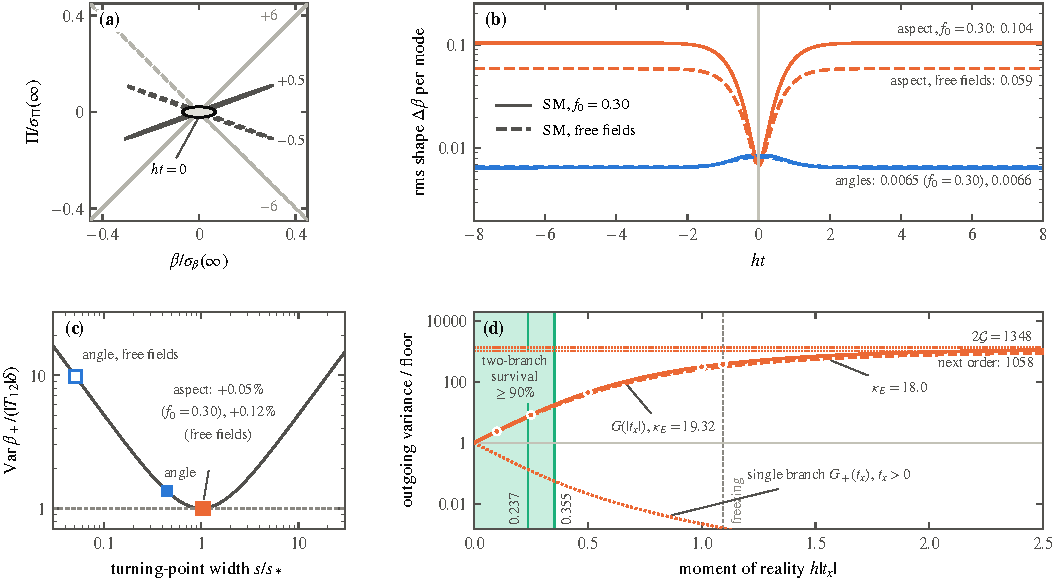
\includegraphics[width=\textwidth]{prd_turning_state}
\caption{The quantum shape through the turning point. (a)~$1\sigma$ Wigner ellipses of the natural state of a Standard Model aspect mode ($\fzm=0.30$) at $ht=0$, $\pm0.5$ and $\pm6$ (past dashed), in outgoing widths. (b)~Rms width of the aspect and angle modes versus time for $\fzm=0.30$ (solid) and free fields (dashed). (c)~Outgoing variance in units of the floor versus the turning-point width, Eq.~\eqref{eq:rA-family}; squares: natural widths (filled: $\fzm=0.30$; open: free fields). (d)~Bound $G(|t_x|)$ for a state real at $t_x$, Eq.~\eqref{eq:rA-Gtx}, at $\kappa_E=19.32$ and $18.0$ (dashed), single-branch bound $G_+$ (dotted), and two-branch survival thresholds $h|t_*|=0.237$ ($99\%$) and $0.355$ ($90\%$, shaded).} %
\label{fig:rA-turning-state}
\end{figure}

\subsection{Time symmetry and the Wheeler--DeWitt wave function}
\label{rA:s-equivalent}

Reality of the shape state at the turn is a statement about the wave function of the universe, and three results make the link precise.

\paragraph{Born--Oppenheimer form.}
Treat the volume semiclassically and the shape in the Born--Oppenheimer approximation.
In the allowed region $L>\Lb$ the wave function then has the form
\begin{equation}
\Psi(L,\beta)=A(L)\big[e^{iS(L)}\chi(\beta,t(L))+e^{-iS(L)}\chi(\beta,-t(L))\big],
\label{eq:rA-WDW}
\end{equation}
where $S(L)$ is the classical action of the volume, $t(L)>0$ is the time at which the classical solution reaches $L$, and $\chi(\beta,t)$, with $i\partial_t\chi=H_s(t)\chi$, is the shape state carried along a single classical history through the turn.
Since $H_s$ is real in the $\beta$ representation and even in $t$, $\chi(-t)^*$ obeys the same equation as $\chi(t)$.

\begin{rAprop}[Reality and the turning-point state]\label{prop:rA-reality}
Within Eq.~\eqref{eq:rA-WDW}, $\Psi$ is real if and only if $\chi(\beta,0)$ is real up to a phase.
\end{rAprop}

\begin{rAproof}
Let $\tilde\chi(t)\equiv\chi(-t)^*$.
Since $H_s$ is real and $H_s(-t)=H_s(t)$, $i\partial_t\tilde\chi=H_s(t)\tilde\chi$ with $\tilde\chi(0)=\chi(0)^*$, so a real $\chi(0)$ gives $\chi(-t)=\chi(t)^*$ at all times and $\Psi=2A\,{\rm Re}[e^{iS}\chi(t)]$ is real.
Conversely, if $\Psi$ is real, the coefficients of the linearly independent factors $e^{\pm iS}$ are complex conjugates, $\chi(\beta,-t)=\chi(\beta,t)^*$, and continuity through the turn along the single history gives $\chi(0)=\chi(0)^*$.
\end{rAproof}

A real $\Psi$ is a standing wave with equal weight on the two branches, which is the two-branch reading.
With CP violation, real reads as invariant under the antiunitary $\Theta=CPT$, which acts as time reversal on the shape modes and the bosonic zero modes.
The single-history condition cannot be dropped: near the turn $\Psi={\rm Ai}(z)\phi_A(\beta)+{\rm Bi}(z)\phi_B(\beta)$, with $z$ the Airy variable of the volume and two different real shape states, is real but carries no real shape state at the turn.
The Airy layer of the volume at the turn has width $\delta\ln L=(144X^2)^{-1/3}=1.1\times10^{-3}$, far below the time scales of the shape. %

\paragraph{Wheeler--DeWitt equation.}
We tested this equivalence on the two-dimensional Wheeler--DeWitt equation for the volume and one aspect mode, including its cubic coupling.
It follows from the minisuperspace action~\eqref{eq:rA-minisuperspace} with the plateau potential frozen at $\phi_b$.
The Hamiltonian constraint reads $-p_L^2/(12\MPbar^2L)+p_\beta^2/(2\MPbar^2L^3)+L^3V(\phi_b)-C(\beta)/L=0$.
We multiply by $12\MPbar^2L^3$, write $x=\ln(L/\Lb)$ with the ordering $L^2p_L^2\to-\partial_x^2$, and use $V(\phi_b)=3\MPbar^2\rAHeff^2$, $\Lb^4=C_b/3\MPbar^2\rAHeff^2$ and $\zeta(\beta)=C(\beta)/C_b$.
With $b=\sqrt X\beta$ the equation becomes
\begin{equation}
\psi_{xx}=6X\psi_{bb}-36X^2\big[e^{6x}-\zeta(b)e^{2x}\big]\psi,\qquad
\zeta=1+\frac{\kappa_E}{6}\beta^2+\frac{c_3}{6}\beta^3,
\label{eq:rA-WDWeq}
\end{equation}
with $\kappa_E=19.3236$ and the cubic coupling $c_3=12.504$ of the twisted Ewald sums. %
The expansion of $\zeta$ follows from that of $Z_{\rm eff}$ in Sec.~\ref{rA:sh-modes}, since $\lambda/[2(1-\fzm)Z_{\rm eff}]=\kappa/6$.
The volume is classically allowed for $x>x_t=\tfrac14\ln\zeta$.
Near $x_t$ the bracket is $4\zeta^{3/2}(x-x_t)$, so the solutions are Airy functions of $z=(x_t-x)/\ell$ with $\ell=(144X^2\zeta^{3/2})^{-1/3}$.

\paragraph{Numerical test.}
We solve Eq.~\eqref{eq:rA-WDWeq} as an initial-value problem in $x$ on a sinc grid of 384 points with $|b|\leq12$, capping the barrier action at 15 for large $|b|$, outside the support of the state. %
Initial data are $\psi={\rm Ai}(z)\phi_A(b)+{\rm Bi}(z)\phi_B(b)$ with $z=(x_t(b)-x)/\ell(b)$.
In the allowed region $\psi\simeq K_0^{-1/2}[e^{iS}\phi_++e^{-iS}\phi_-]$ with $K_0=6Xe^{3x}(1-e^{-4x})^{1/2}$, the local wave number for $\zeta=1$, so $\phi_\pm=(\psi\mp i\psi_x/K_0)\sqrt{K_0}/2$, and each branch is evolved back to the turn with the shape Hamiltonian
\begin{equation}
H_s=-\frac{\partial_b^2}{2e^{3x}}-3Xe^{-x}(\zeta-1),
\end{equation}
which is $p_\beta^2/(2\MPbar^2L^3)-C_b(\zeta-1)/L$ in units of $\rAHeff$.
From the two reconstructed states we form the single-history defect $D_{\rm sh}=1-|\langle\chi_{\rm con}|\chi_{\rm exp}\rangle|/(\|\chi_{\rm con}\|\|\chi_{\rm exp}\|)$ and the reality defect $D_{\rm re}=1-|\sum\chi_{\rm exp}^2|/\sum|\chi_{\rm exp}|^2$.
For real $\Psi$ the time-reversal property forces $D_{\rm sh}=D_{\rm re}$, which every run with real data reproduces digit by digit.
For real data that decay under the Casimir barrier, the Ai-type solutions favored by no-boundary regularity, the reconstructed state is real up to a defect $D_{\rm re}=3.1\times10^{-2}$, $4.3\times10^{-4}$, $1.5\times10^{-5}$ and $2.4\times10^{-6}$ at $X=100$, $300$, $1000$ and the physical $2282$. %
The defect falls roughly as $X^{-2.4}$. %
These defects hold at the three extraction times $t=0.3$, $0.45$ and $0.6$, and the fidelity with the declared profile approaches 1 as $X^{-0.8}$, from $0.93$ at $X=100$ to $0.996$ at $X=2282.49$. %
For two real profiles the Born--Oppenheimer reading gives $\chi(0)\propto i\phi_A+\phi_B$, hence
\begin{equation}
D_{\rm re}=1-\frac{\big|\|\phi_B\|^2-\|\phi_A\|^2+2i\langle\phi_A,\phi_B\rangle\big|}{\|\phi_A\|^2+\|\phi_B\|^2}.
\end{equation}
For the counterexample with Bi weight $\eta$ and an orthogonal shape state, the defect approaches the Born--Oppenheimer prediction $2\eta^2/(1+\eta^2)$: it is $0.969$ at $\eta=1$, and $0.161$ at $\eta=0.3$ against the predicted $0.165$. %
With $\phi_B\parallel\phi_A$, $({\rm Ai}+0.7\,{\rm Bi})\otimes\chi_0$ gives $D_{\rm re}=5.0\times10^{-4}$. %
A complex shape state gives a complex $\Psi$ and a complex reconstructed state, the contrapositive of the equivalence.
The equivalence therefore holds when the Ai and Bi components carry the same shape state, and decay under the barrier is a sufficient condition.
A Bi component with a different shape state would need exponential tuning, because the barrier action is $S_E\simeq5.24X\simeq1.2\times10^4$ (Sec.~\ref{rA:c-size}). %

\paragraph{A selection rule.}
A rule that maps the data at the turning point to a quantum state, covariantly under $\Theta$ and with a unique outcome, gives a $\Theta$-invariant, hence real, state, because those data ($K_{ij}=0$, the cubic shape, the AAA spin structure) are $\Theta$ invariant.
Rules that pick an instantaneous ground state belong to this class.
So does the Hartle--Hawking proposal~\cite{Hartle:1983ai} when its saddle and integration contour are $\Theta$ symmetric.
The CPT-symmetric proposal of Boyle, Finn and Turok~\cite{Boyle:2018tzc} is an analog in a different setting.
The tunneling proposal~\cite{Vilenkin:1984wp} is not in the class, because its outgoing boundary condition picks a direction of time.
Under the conditions above, a fossil measured well below the floor would exclude the $\Theta$-real class: that class gives a fossil at or above the floor, and at the floor for the natural state, whereas an outgoing state has no lower bound on our branch and reaches $0.2\%$ of the floor in variance for reality one Hubble time after the turn. %
A single torus measures $\ln\sigma_E$ to about $\pm0.5$ (Sec.~\ref{rA:c-tests}), enough to separate the floor from a state that becomes real later than about $0.25/h$ after the turn, but not from one real at $0.1/h$. %
Where uniqueness fails, as for the Euclidean continuation of Sec.~\ref{rA:s-euclid}, reality is an additional postulate, equivalent to the two-branch reading itself; arrows of time and boundary conditions of quantum cosmology were related in this spirit in Refs.~\cite{Hawking:1985af,Page:1985ei,Kiefer:1994gp}.

\paragraph{Minimal energy variance.}
The natural state has a characterization of its own.

\begin{rAprop}[Minimal energy variance]\label{prop:rA-minvar}
Consider the inverted oscillator $H=p^2/2m-kx^2/2$ and the pure centered Gaussians $\psi\propto\exp[-(a-ib)x^2]$.
Among these states the energy variance is at least $k/2m$.
The minimum is attained along one dynamical orbit, and its unique time-reflection-invariant member has $\langle x^2\rangle=1/(2m|\omega|)$ with $|\omega|=(k/m)^{1/2}$, the natural width of Sec.~\ref{rA:s-natural}.
\end{rAprop}

\begin{rAproof}
For this Gaussian $\langle x^2\rangle=1/4a$, and a direct computation of $\langle H^2\rangle-\langle H\rangle^2$ gives
\begin{equation}
\rAVar\,H=\frac{16a^4+32a^2b^2+8a^2km+16b^4-8b^2km+k^2m^2}{32a^2m^2}.
\end{equation}
At $b=0$ the numerator is $(4a^2+km)^2$, and $(4a^2+km)/a$ is minimal at $a=\sqrt{km}/2$, that is $\langle x^2\rangle=1/(2m|\omega|)$, where $\rAVar\,H=k/2m$.
For $|b|<\sqrt{km}/2$ the same value is reached at $a=(km-4b^2)^{1/2}/2$, where the numerator becomes $4km(km-4b^2)$ and the denominator $8m^2(km-4b^2)$; this one-parameter set is the orbit of the natural state under the inverted-oscillator evolution, and $b=0$ is its only time-reflection-invariant member.
\end{rAproof}

A symbolic computation confirms these expressions. %
The natural state is therefore the time-symmetric Gaussian of minimal energy variance; outside the Gaussian family real states can have arbitrarily small energy variance.

\subsection{The quantum fossil}
\label{rA:s-fossil}

After a few Hubble times the Casimir force, which decays as $L^{-4}$ relative to the inertia, switches off and the shape freezes~\cite{Fornal:2026qfq}.
Its outgoing distribution is the quantum fossil of the turning point, listed in Table~\ref{tab:rA-fossil} for the $A_s$-calibrated plateau history.

\begin{table}[tbp]
\centering
\caption{Rms outgoing shape per mode for the natural state at the turn (assumption~\ref{assump:A8}): the quantum floor of the aspect ($E$) modes, Eq.~\eqref{eq:rA-floor}, and the natural width of the angle ($T_2$) modes, with the aspect stiffness and gain and the typical difference between the longest and shortest sides. The variances of the natural aspect states exceed the floor by $0.05\%$ ($\fzm=0.30$), $0.12\%$ (free fields) and $0.87\%$ (toy). Standard Model rows use the AAA spin structure.} %
\label{tab:rA-fossil}
\begin{tabular}{lccccc}
\toprule
 & $\kappa_E$ & $\rAGain$ & $\sfloor$ & $\sigma_{T_2}$ & sides\\
\midrule
SM, $\fzm=0.30$ & 19.32 & 674 & 0.104 & 0.0065 & $18\%$\\ %
SM, next order & 18.0 & 529 & 0.0934 & --- & $16\%$\\ %
SM, free fields & 13.53 & 216.5 & 0.0587 & 0.0066 & $10\%$\\ %
Maxwell toy & 6.00 & 30.6 & 0.0178 & 0.0069 & ---\\ %
\bottomrule
\end{tabular}
\end{table} %

\paragraph{The frozen box.}
For the Standard Model the fundamental domain is an almost rectangular box [Fig.~\ref{fig:rA-fossil}].
With $\fzm=0.30$ the rms of $\ln(L_i/L_j)$ is $\sqrt2\,\sigma_E=0.147$, by Eq.~\eqref{eq:rA-aspect}. %
The median of $\ln(L_{\max}/L_{\min})$ is $1.588\,\sigma_E$, so the longest and shortest sides typically differ by $18\%$ at leading order and by $16\%$ with the next-order corrections, against $10\%$ for free fields. %
Each edge angle deviates from $90^\circ$ by $\sqrt2\,\sigma_{T_2}=0.53^\circ$ rms. %

\paragraph{Scaling.}
The aspect fossil obeys $\sigma_E^2=\delta|\rATm_{12}(\kappa_E)|$, so fewer light fields and a stronger instability give a larger fossil; at the Standard Model value $d\ln\sigma_E/d\ln\kappa_E=1.37$, which follows from Eq.~\eqref{eq:rA-T12b} at fixed $X$. %
With $\delta\propto1/X$ and $X=(\rANeff\rAgam/3)^{3/4}(\MPbar/\rAHeff)^{1/2}$, $\sigma_E\propto(\rAHeff/\MPbar)^{1/4}(\rANeff)^{-3/8}\rATm_{12}^{1/2}$.
For plateau inflation $\rAHeff/\MPbar\propto(A_s\rT)^{1/2}$, with $\rT$ the tensor-to-scalar ratio (Sec.~\ref{rep:spectra}), so that
\begin{equation}
\sigma_E\propto(A_s\rT)^{1/8}\,(\rANeff)^{-3/8}\,\rATm_{12}(\kappa_E)^{1/2},
\label{eq:rA-scaling}
\end{equation}
where $\kappa_E$ also depends on the field content.
At fixed content this relates a measurement of the tensor ratio to the predicted shape: measuring $\rT\simeq0.004$ to $\pm10^{-3}$ fixes $\sigma_E$ to $\tfrac18\times\tfrac14=3.1\%$. %

\paragraph{Fossil anisotropy.}
The net change of the shape between the far past and the far future, $\beta_+-\beta_-$, is the fossil anisotropy that Ref.~\cite{Zhou:2026szo} introduced for anisotropic flat cosmologies.
Here it is computed for a quantum state; since $\beta_-$ and $\beta_+$ are nearly uncorrelated and have equal variances by time symmetry, its rms is $1.39\,\sigma_E$ per aspect mode, close to $\sqrt2\,\sigma_E$. %

\paragraph{Next order.}
The next-order terms of the zero-mode energy (Sec.~\ref{rA:zm-shape}) lower $\fzm$ to about $0.28$ and $\kappa_E$ to $18.0$. %
They lower the gain from $674$ to $529$, the saturated amplification $G(\infty)$ from $1348$ to $1058$, and the floor by the factor $0.900$, from $0.1037$ to $0.0934$. %
The energy and the Hessian contribute factors $0.953$ and $0.945$ to this decrease. %
Through $G$ the next order moves the conditional threshold outward, from $h|t_*|=0.237$ to $0.265$ at the $99\%$ level, and raises the survival of real states set in the frozen region from $13$--$18\%$ to $17$--$23\%$. %
We quote leading-order values and treat the next-order shift as a one-sided uncertainty; higher orders are not estimated.

\paragraph{Error budget.}
The numerical error of $\sigma_E$ is below $0.1\%$. %
Classical nonlinear evolution raises the aspect variance by factors $1.043$ and $1.045$ in two sets of $2048$ draws, and by $1.032$ in an independent implementation (Sec.~\ref{rA:s-nonlinear}). %
The leading quantum correction beyond the truncated Wigner evolution, the Moyal term, changes the aspect variance by $-0.020\%$ and the angle variance by $-0.11\%$. %
Including the inflaton fluctuation in $\NC$ lowers $\sigma_E$ by $3.5\%$, and the weak-decay calibration of $h$ instead of instant reheating raises it by $2.5\%$. %
A shift of $0.02$ in $\fzm$ moves $\sigma_E$ by $5\%$, and the next order lowers it by $10\%$. %
Evaluating $X$ with the plateau parameter $h$ instead of $\rAHeff$, or mixing the two, moves $\sfloor$ within $0.1031$--$0.1041$. %
The convention for the initial momentum at finite amplitude changes individual draws by $0.8\%$ rms. %

\begin{figure}[tbp]
\centering
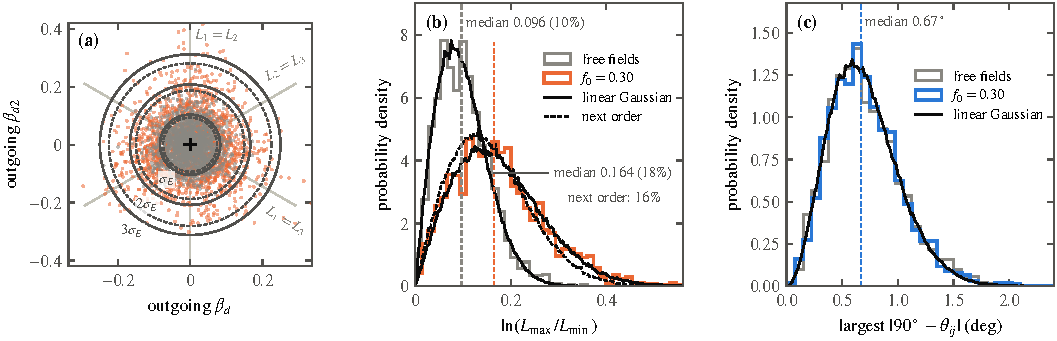
\includegraphics[width=\textwidth]{prd_fossil_shape}
\caption{Frozen shape of the torus after a Standard Model turning point. (a)~Outgoing aspect coordinates of $2048$ natural turning-point states with $\fzm=0.30$ (orange) and $2048$ for free fields (gray), evolved through the full nonlinear equations; circles: $1$, $2$ and $3\sigma_E$ of the linear prediction at leading (solid) and next order (dashed, $\sigma_E=0.0934$); gray lines: two equal sides. (b)~Logarithm of the ratio of the longest to the shortest side, $\ln(L_{\max}/L_{\min})$, and (c)~largest deviation of an edge angle from $90^\circ$, for the nonlinear draws (steps) and the linear Gaussian (lines; dashed in (b): next order).} %
\label{fig:rA-fossil}
\end{figure}

\subsection{Nonlinear evolution and corrections}
\label{rA:s-nonlinear}

Classical nonlinear shape dynamics leave the fossil of a state real at the turn intact, but they end the shape when the outgoing deformation is large.

\paragraph{Equations.}
With $K=\tfrac12\dot G$, $\sigma=G^{-1}K$ and $\mathsf Y=(L/\Lb)^3K$, the leading equations are
\begin{equation}
\dot L=HL,\qquad \dot H=2h^2-2H^2-\tfrac16\Tr\sigma^2,\qquad \dot G=2K,\qquad \dot{\mathsf Y}=2\Big(\frac{\Lb}{L}\Big)^3\mathsf YG^{-1}\mathsf Y+\Big(\frac{L}{\Lb}\Big)^3G\mathsf F,
\label{eq:rA-nl-eqs}
\end{equation}
where $\mathsf F$ is the trace-free Casimir shape force from range-adaptive Ewald sums.
The equation for $\dot H$ follows from Eq.~\eqref{eq:rA-einstein} with $\rho+\bar p=\tfrac43\rho_C$ for the traceless Casimir stress, after $\rho_C=3\MPbar^2(H^2-h^2)-\tfrac12\MPbar^2S$ is eliminated with the constraint; it holds for every shape.
The Friedmann constraint, $\det G=1$ and $\Tr G^{-1}\mathsf Y=0$ are conserved and serve as accuracy gates.

\paragraph{Standard Model forces and initial data.}
For the AAA Standard Model the force is the unimodular gradient of $Z_{\rm eff}=15Z_2(G,0)-45Z_2(G,\bm\vartheta_F)$, the 15 periodic bosonic and 45 antiperiodic Weyl degrees of freedom, which matches finite differences of $Z_{\rm eff}$ to $10^{-11}$. %
Each draw starts at the turning point with $\beta_A$ and $\Pi_A$ sampled from the Wigner function of the chosen Gaussian, $G_0=\exp(2\sum\beta_AX_A)$, the momentum $G_0^{1/2}(\sum_A\Pi_AX_A)G_0^{1/2}$ up to the normalization of Eq.~\eqref{eq:rA-delta}, and the turning-point size from the constraint at $H=0$.
A shape-independent ground energy $Q/L=\fzm C/L$ enters only through the constraint, $Z_{\rm eff}(G)\to Z_{\rm eff}(G)-\fzm Z_{\rm eff}(\rAone)$, and leaves the force unchanged; with it $\kappa_A\to\kappa_A/(1-\fzm)$ and $\delta\to\delta(1-\fzm)^{-3/4}$.
A draw survives if it reaches $ht=12$ without recollapse, with the smallest eigenvalue of $G$ above $10^{-3}$ throughout and $H>0.9\,h$ at the end. %

\paragraph{Integration and controls.}
We integrate with an eighth-order Runge--Kutta method at relative tolerance $10^{-11}$; small-amplitude runs reproduce the linear transfer to $2\times10^{-9}$, and the gates hold to $7\times10^{-11}$ for the natural states. %
Enlarging the Ewald cutoff by $40\%$, relaxing the tolerance to $10^{-9}$, or deepening the collapse criterion to $10^{-6}$ changes no fate among the draws tested. %
The evolution is a truncated Wigner approximation: it is exact at linear order and omits the Moyal terms, and the volume and inflaton are classical.
Convergence studies of these runs are collected in Sec.~\ref{rep:v-convergence}.

\paragraph{Natural states.}
We drew phase-space points from the Wigner function of the natural Standard Model state and evolved each through the full equations for $L$ and the five-dimensional $G$, with twisted Ewald forces, on the turning-point solution.
For free fields all $128$ and $2048$ draws survive, and their outgoing aspect variances exceed those of the same draws under the linear transfer by factors $1.016$ and $1.012$. %
Of 64 free-field draws with amplitudes scaled by $3$, $5$, $8$ and $12$, all, $63$, $54$ and $44$ survive, and the 2048 natural draws give $\langle\Tr B^3\rangle/\langle\Tr B^2\rangle^{3/2}=-0.07\pm0.03$ for $B=\sum\beta_{A,+}X_A$, a slight preference for two long sides and one short one. %
With $\fzm=0.30$ two sets of $2048$ draws, one reusing the normal deviates of the free-field draws and one with an independent seed, all survive, with factors $1.043$ and $1.045$ ($95\%$ intervals $1.033$--$1.054$ and $1.035$--$1.055$) for the aspect modes and $0.998$ and $1.004$ for the angle modes, and individual shapes move by $8$--$9\%$ rms ($8.6\%$ and $8.3\%$). %
The median of $\ln(L_{\max}/L_{\min})$ is then $0.164$, against $0.165$ for the linear Gaussian. %
An independent implementation gives $1.032$ ($1.023$--$1.040$); the $1.5\sigma$ difference is consistent with the convention for the initial momentum at finite amplitude. %

\paragraph{How large states fail.}
Larger states fail in one way.
The volume turns at $t\simeq0$, and then one cycle is squeezed to zero within $0.3$--$4$ Hubble times; the smallest eigenvalue of $G$ falls from $10^{-3}$ to $10^{-6}$ in at most $0.007/h$, a finite-time singularity of the shape. %
Every failure but those at the largest amplitudes is a collapse of one cycle after the volume has turned: in the independent implementation $H$ crosses zero when the smallest eigenvalue of $G$ is near $0.04$, and the eigenvalue reaches zero about $0.04/h$ later. %
The volume fails to turn only for states at least $20$ times wider than the natural one, or real at $ht_x\leq-2$, in at most $3\%$ of the draws there. %

\paragraph{Amplitude scans.}
Table~\ref{tab:rA-amp} collects the survival of the natural state scaled by $s$ at $\fzm=0.30$, from our main code with 256 draws per point, a second run with 2048 draws near the $99\%$ level, and an independent implementation with its own Ewald sums, integrator and seeds. %
Scaling the natural state by a factor $s$, the independent implementation with $2048$ draws each gives survival $1.000$, $0.987$, $0.818$, $0.365$, $0.067$ and $0.0015$ for $s=1$, $3$, $5$, $10$, $20$ and $40$, in agreement with our main runs with $256$ draws per point [Fig.~\ref{fig:rA-survival}(a)]. %
Half of the trajectories survive up to $s_{50}=8.2$ and $90\%$ up to $s_{90}=4.2$--$4.3$. %
Linear interpolation in $\ln s$ between the nodes of the 2048-draw run gives $s_{99}=2.76$ ($95\%$ interval $2.66$--$2.90$), a logistic fit $2.86$ ($2.74$--$2.96$), and the $1\%$ quantile of the critical amplification of single draws in the independent run $2.95$. %
The $99\%$ level therefore lies at $s_{99}\simeq2.8$--$2.95$, a range that spans interpolation, a logistic fit and the quantiles of the critical amplification of single draws. %
The 2048-draw value of $S(3)$, $0.9834\pm0.0028$, and the independent $0.987$ differ by about $2\sigma$, which accounts for the spread. %
In terms of the outgoing linear amplitude, $99\%$ of the trajectories survive below $\sigma_{\rm lin}\simeq0.29$--$0.31$ per aspect mode, and half below $0.85$--$0.89$. %
At next order the same procedure gives $s_{99}=3.16$ (logistic $3.29$), $s_{90}=4.19$ and $s_{50}=9.07$. %
Free fields tolerate more: every draw survives up to three times the natural amplitude, while with $\fzm=0.30$ that amplitude keeps $97$--$99\%$ of the trajectories. %

\begin{table}[tbp]
\centering
\caption{Survival of the natural turning-point state scaled by $s$, at $\fzm=0.30$: runs of our main code with 256 and 2048 draws per point, an independent implementation with 2048 draws, and the rms outgoing aspect amplitude $\sigma_{\rm lin}$ of the linear images of the sampled draws.}
\label{tab:rA-amp}
\begin{tabular}{lcccc}
\toprule
$s$ & 256 draws & 2048 draws & independent & $\sigma_{\rm lin}$\\
\midrule
1 & 1.000 & --- & 1.000 & 0.109\\ %
2.5 & --- & 0.9976 & --- & 0.262\\ %
3 & 0.973 & 0.9834 & 0.987 & 0.314\\ %
3.5 & --- & 0.9536 & --- & 0.366\\ %
5 & 0.824 & --- & 0.818 & 0.543\\ %
10 & 0.367 & --- & 0.365 & 1.085\\ %
20 & 0.062 & --- & 0.067 & 2.171\\ %
40 & 0.000 & --- & 0.0015 & 4.342\\ %
\bottomrule
\end{tabular}
\end{table}

\paragraph{One survival curve.}
Survival is mainly a function of $\sigma_{\rm lin}$.
For $\sigma_{\rm lin}\lesssim1.5$ the amplitude scans at three stiffnesses, the real states of Sec.~\ref{rA:s-conditional}, the phase and adiabatic families and the outgoing never-real states lie on one curve to within $\pm5$ percentage points. %
The comparison of Tables~\ref{tab:rA-S2} and~\ref{tab:rA-amp} shows the same: a real state at $h|t_x|=0.25$ has $\sigma_{\rm lin}=0.297$ and survives with $0.987$, as does the natural state scaled by $s=3$, with $\sigma_{\rm lin}=0.314$.

\begin{figure}[tbp]
\centering
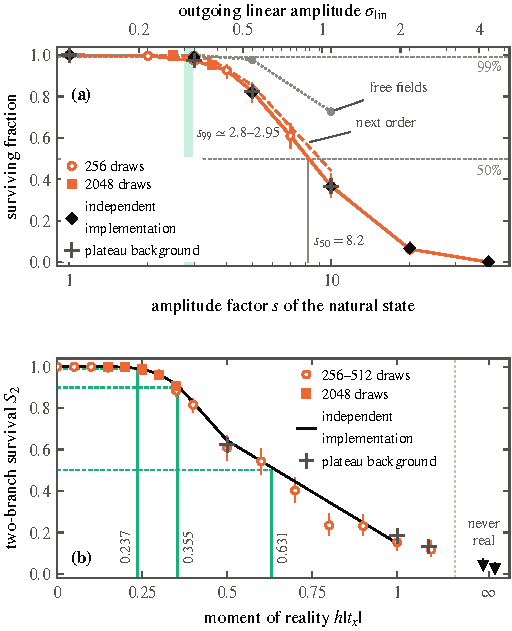
\includegraphics[width=0.8\textwidth]{prd_nonlinear_survival}
\caption{Shape survival through a Standard Model turning point with $\fzm=0.30$. (a)~Surviving fraction when the natural turning-point state is scaled by $s$: runs with $256$ and $2048$ draws per point, an independent implementation (diamonds), the same draws on the $A_s$-calibrated plateau background (crosses), next order (dashed), and free fields (dotted); upper axis: outgoing linear amplitude $\sigma_{\rm lin}$; band: $s_{99}\simeq2.8$--$2.95$. (b)~Two-branch survival $S_2$ of the optimal real Gaussian versus the moment of reality $h|t_x|$, with an independent implementation (line), plateau-background states (crosses), never-real pairs ($\infty$), and the thresholds $0.237$, $0.355$, and $0.631$ for $99\%$, $90\%$, and $50\%$. Wilson $95\%$ intervals.} %
\label{fig:rA-survival}
\end{figure}

\paragraph{Moyal correction.}
Quantum corrections are small.
Expanding $Z_{\rm eff}/Z_{\rm eff}(\rAone)$ to third order at the cube, with tensor $c_{ABC}$, the second moments of the quantum and the truncated Wigner evolution differ first at order $c^2$, through the third-derivative term of the Moyal bracket:
\begin{equation}
\Delta\rAVar\,q_A=-\frac{\delta^2}{2}\iint dt\,dt'\,W_A(t)W_A(t')\sum_{BC}c_{ABC}^2\,r_B(t,t')\,r_C(t,t'),
\end{equation}
with $r_B(t,t')=f_B(t)g_B(t')-g_B(t)f_B(t')$ built from the fundamental solutions $f,g$ of each mode, $W_A(t)=V(t)\,r_A(T,t)$ and $V=-3/(cL)$ in the units of Sec.~\ref{rA:s-quantization}.
The correction depends on the window over which the state evolves quantum mechanically, not on the initial state, and quartic terms give no quantum-classical difference at this order.
For the AAA Standard Model at $\fzm=0.30$ the three independent cubic constants are $c_{E^3}=12.50$, $c_{ET_2^2}=7.91$ and $c_{T_2^3}=-5.57$, five times those of the Maxwell toy. %
For the Standard Model with a state real at the turn it changes the aspect variance by $-0.020\%$ and the angle variance by $-0.11\%$. %
This is $28$ times less than for the Maxwell toy prepared twelve Hubble times before the turn; on that window the Standard Model value is $-1.0\%$. %
For real states set before the turn it is $-0.07\%$ to $-0.51\%$. %
An independent implementation reproduces the earlier Maxwell-toy coefficient to $1.2\times10^{-7}$, and an exact split-operator evolution of a single mode agrees with the formula to $0.35\%$, $1.4\%$ and $5.8\%$ at half, one and two times the Standard Model coupling, a deviation that grows as $c^2$. %
At next order the aspect and angle corrections become $-1.79\times10^{-4}$ and $-9.2\times10^{-4}$. %
These bounds concern second moments; the survival fractions, set by trajectories near collapse, are not constrained by them.

\paragraph{Plateau background.}
To test the leading solution we replaced it by the time-symmetric plateau history with a homogeneous rolling inflaton, $\hat V(\phi)=3[(1-e^{-a\phi})/(1-e^{-a\phi_b})]^2$ with $a=\sqrt{2/3}$ and $\phi_b=5.5794$, in units of $\MPbar^2\rAHeff^2$. %
The turning-point data at $t=0$ are identical, and for $\phi_b\to\infty$ the code reproduces the leading-solution runs to $1.4\times10^{-14}$. %
Replacing the leading turning-point solution by this history changes the linear gains by $+3$--$4\times10^{-4}$ and, in $2560$ trajectories paired with the leading-solution runs, at $s=1$, $3$, $5$ and $10$ and for real states at $ht_x=-0.5$, $-1$ and the onset of freezing, the fate of none. %
The outgoing shapes of common survivors differ by a median of $1.5$--$3.4\times10^{-4}$ in relative terms. %
The independent implementation, run on a second reference plateau with $\phi_b=5.587$, finds survival higher by $0.4$--$0.8$ percentage points, all from draws that survive on the plateau and fail on the leading solution. %
For the Maxwell toy the backreaction of the shape moments on the volume and inflaton shifts $N_{\rm post}$ by $-5\times10^{-4}$ and the aspect variance by $+0.05\%$. %

\paragraph{Shear criterion.}
At the turning point $H=0$, and the constraint fixes $u\equiv(L/\Lb)^2$.
With $\zeta=Z_{\rm eff}(G_0)/Z_{\rm eff}(\rAone)$ and $s_0=\Tr[(G_0^{-1}\mathsf Y_0)^2]$ in the units of Eq.~\eqref{eq:rA-nl-eqs}, the shear at the turn is $S=s_0h^2/u^3$ and the constraint, multiplied by $u^2/3\MPbar^2h^2$, reads
\begin{equation}
u^2+\frac{s_0}{6u}=\zeta .
\end{equation}
The left side has its minimum $3(s_0/12)^{2/3}$ at $u^3=s_0/12$, so a large-volume root exists if and only if $s_0\leq12(\zeta/3)^{3/2}$.
Along a single direction this predicts the critical momentum $p_c=1.43276$, and the integration turns at $0.99\,p_c$ and fails at $1.01\,p_c$. %
Near the cube, $\zeta\simeq1$, the criterion is $\rho\equiv s_0/12<3^{-3/2}=0.19245$: a trajectory has turning-point data only if its shape momenta obey $\sum_AP_A^2<12\cdot3^{-3/2}\,\MPbar^4\Lb^6\rAHeff^2$. %
States set in an adiabatic vacuum ($\omega=c_\omega|H|$) at the onset of the plateau contraction violate it on average after $N_{\rm pre}=1.32$ ($c_\omega=1$) and $1.01$ ($c_\omega=3$) e-folds of contraction, whereas optimal-width real states keep the mean ratio below $0.112$. %
For fixed shape momenta, which are conserved across the thin turning layer, the volume obeys the Wheeler--DeWitt equation
\begin{equation}
\psi''(x)+12X^2\Big[3e^{6x}-3\zeta e^{2x}+\frac{s_0}2\Big]\psi=0,\qquad x=\ln(L/\Lb),
\end{equation}
which is Eq.~\eqref{eq:rA-WDWeq} with $6p_\beta^2\to6s_0X^2$.
A uniform parabolic-cylinder approximation gives the collapse probability $1/\{1+\exp[24.81X(\rho_c-\rho)]\}$, which numerical scattering confirms for $X=30$--$2282.49$ with errors falling as $1/X$. %
At $X=2282.49$ the criterion moves by $3.5\times10^{-8}$ in relative terms, and its 10--90\% width is $\Delta\rho=7.8\times10^{-5}$, or $4\times10^{-4}$ relative. %
A quantum treatment of the volume therefore turns the classical step into a smooth one of relative width $4\times10^{-4}$ without moving it. %

\subsection{Why a Euclidean continuation does not fix the state}
\label{rA:s-euclid}

A no-boundary prescription is the natural candidate for selecting the turning-point state.
Continuing $t=-i\tau$, $\tanh2ht\to-i\tan2h\tau$, ${\rm sech}^22ht\to\sec^22h\tau$ and $d/dt\to i\,d/d\tau$, Eq.~\eqref{eq:rA-shapeode} becomes
\begin{equation}
\beta''-3h\tan(2h\tau)\beta'+\kappa h^2\sec^2(2h\tau)\beta=0 .
\end{equation}
This reaches the singular end $L_E=\Lb\sqrt{\cos2h\tau}\to0$ of the Euclidean solution, at $h\tau_0=\pi/4$, which Ref.~\cite{Guth:2025dal} rejects as an instanton.
Near that end, with $s=\tau_0-\tau\to0$, $\tan2h\tau\simeq1/2hs$ and $\sec^22h\tau\simeq1/4h^2s^2$, and the continued equation becomes
\begin{equation}
\beta_{ss}+\frac{3}{2s}\beta_s+\frac{\kappa}{4s^2}\beta=0,
\end{equation}
with solutions $s^p$ and exponents
\begin{equation}
p=-\tfrac14\pm\tfrac14\sqrt{1-4\kappa}.
\end{equation}
The quadratic action $\tfrac12\int ds\,(s^{3/2}\beta_s^2-\tfrac\kappa4s^{-1/2}\beta^2)$, whose Euler--Lagrange equation is the one above, reduces on shell to the boundary term $\tfrac12s^{3/2}\beta\beta_s\propto s^{2p+1/2}$.
For $\kappa<1/4$ only the larger exponent keeps it finite and selects the state.
For $\kappa>1/4$ both have ${\rm Re}\,p=-1/4$ and oscillate log-periodically with the same amplitude, with period $\Delta\ln s=8\pi/\sqrt{4\kappa-1}$.
The kinetic and potential parts each diverge logarithmically, but their sum stays bounded and oscillates without a limit at the singular end, so regularity selects neither solution.
A direct integration toward $\tau_0$ reproduces the predicted number of sign changes for $\kappa=6.0$, $13.5$ and $8/5$ and finds none for $\kappa\leq1/4$. %
Since some $\kappa_A\geq8/5$, every Casimir turning point has such a mode, and the Euclidean continuation of the isotropic turning point selects no shape state.
Real tunneling geometries, compact Euclidean geometries joined to Lorentzian ones across a surface of vanishing extrinsic curvature, carry the no-boundary predictions for the large-scale topology~\cite{Gibbons:1990ns}; the turning point has $K_{ij}=0$, but its singular Euclidean continuation is not of this kind.

The no-boundary saddles of a three-torus found in Ref.~\cite{Godet:2026gqw} are complex, cap one cycle smoothly and have no turning point.
Joining such a cap to the Casimir turning point needs the one-loop stress on a cigar times a two-torus, where the homogeneous Casimir formula fails.
That failure marks the precision of the homogeneous model rather than an obstruction: the stress in the flat core is finite, and on a curved cigar the negative aspect kernel keeps its sign (Sec.~\ref{rep:v-conditional}).
Whether a self-consistent capped saddle exists, and where it would center the shape, remains open.
A classical offset of the mean shape grows by $m_{11}=10.6$ through the turn, so it must stay below about $0.01$, or $1.4$ quantum widths of the natural state ($\beta_{\rm rms}=0.0071$), for the quantum fossil to dominate. %

\section{Primordial spectra}\label{rep:spectra}

The turning point leaves no feature in the primordial spectra.
Every mode of the torus is deep inside the Hubble radius at the turn and starts in its adiabatic vacuum, which evolves into the Bunch--Davies state of the plateau.
The scalar tilt and the tensor-to-scalar ratio $\rT$ are therefore those of the plateau potential, Eq.~\eqref{eq:rA-plateau}, at the number of $e$-folds fixed by reheating.
Through the scale of inflation the spectra also enter the two observable consequences of the turn, the shape fossil and the Higgs criterion, but only weakly.
Section~\ref{rA:c-nofeature} treats tensors and scalars through the turn, Sec.~\ref{rA:c-tilt} the tilt and the tensor ratio, and Sec.~\ref{rA:c-scale} what the tensor ratio fixes.

\begin{figure}[tbp]
\centering
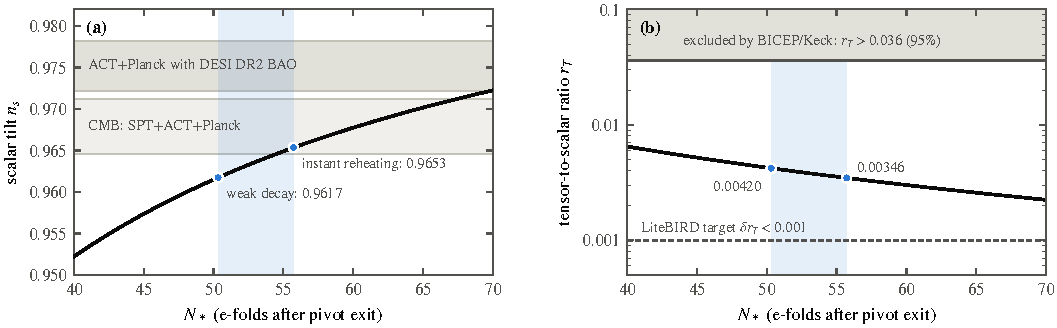
\includegraphics[width=\textwidth]{prd_primordial}
\caption{Primordial tilt and tensor ratio of the plateau potential, which the turning point leaves intact. (a)~Scalar tilt versus the number $N_*$ of $e$-folds between pivot exit and the end of inflation; the colored band spans the weak visible decay ($N_*=50.33$) and instant reheating ($55.72$). Gray bands: $68\%$ intervals from SPT-3G, ACT and Planck CMB data (CMB-SPA)~\cite{SPT-3G:2025bzu} and from ACT and Planck with CMB lensing and DESI DR2 baryon acoustic oscillations (P-ACT-LB2)~\cite{AtacamaCosmologyTelescope:2025blo,DESI:2025zgx}. (b)~Tensor-to-scalar ratio $\rT$ with the BICEP/Keck bound~\cite{BICEP:2021xfz} and the LiteBIRD target~\cite{LiteBIRD:2022cnt}.} %
\label{fig:rA-primordial}
\end{figure}

\subsection{No feature from the turning point}
\label{rA:c-nofeature}

All modes of the torus are inside the Hubble radius at the turn by at least a factor $k/(a_bh)=2\pi|\bm n|/(h\Lb)\geq2\pi/(h\Lb)\simeq1400$ (1300 for free fields), and the emptiness gate of Sec.~\ref{rep:gate} puts them in their adiabatic vacuum there. %
That vacuum evolves into the Bunch--Davies state of the subsequent plateau, with Bogoliubov coefficients suppressed by powers of $h\Lb/2\pi|\bm n|$.

\paragraph{Tensors.}
Free tensor modes $h_{\bm k}=v/a$ on the turning-point solution, Eq.~\eqref{eq:rA-turning-solution}, obey $v''+(k^2-a''/a)v=0$ with $a''/a=2h^2a^2$ exactly (Eq.~\eqref{eq:rA-app}).
With the lemniscatic form of the scale factor, Eq.~\eqref{eq:rA-lemniscatic}, $a^2=\Lb^2\wp(z)$ with $z=h\Lb(\eta-\eta_0)$ and invariants $g_2=4$, $g_3=0$, this is Lam\'e's equation with $n(n+1)=2$,
\begin{equation}
\frac{d^2v}{dz^2}=\Big[2\wp(z)-\frac{k^2}{(h\Lb)^2}\Big]v ,
\label{eq:rA-lame}
\end{equation}
the flat counterpart of the closed universe with radiation and a positive cosmological constant treated in Ref.~\cite{Sarangi:2006yy}.
For $n=1$ the solutions are known in closed form: Hermite's functions $v=\sigma(z+\alpha)\,e^{-z\zeta(\alpha)}/\sigma(z)$, with the Weierstrass functions $\sigma$ and $\zeta$, solve $v''=[2\wp(z)+\wp(\alpha)]v$, as follows from $(\ln v)''+[(\ln v)']^2$ and the addition theorem $[\zeta(z+\alpha)-\zeta(z)-\zeta(\alpha)]^2=\wp(z+\alpha)+\wp(z)+\wp(\alpha)$; here $\wp(\alpha)=-k^2/(h\Lb)^2$.
They are the Floquet (Bloch) solutions of Eq.~\eqref{eq:rA-lame}.
The far past and the far future are the two poles of $\wp$ that bound the real period, where $v\propto z^{-1}$ or $z^2$, the frozen and the decaying tensor mode of de~Sitter space.
For a ground state set at the turn, the late tensor power differs from that of the Bloch state of Lam\'e's equation, defined by its Floquet solutions, by $1.7\times10^{-6}$ at $k/(a_bh)=727$, below the lowest torus mode, and by $2\times10^{-7}$ at $2300$. %

\paragraph{Scalars.}
For scalars the variable $z_{\rm MS}=a\dot\phi/H$ of the Mukhanov--Sasaki equation is $0/0$ at $H=\dot\phi=0$, and its finite limit does not describe the inflaton at the turn.
A finite limit does not license the single-field equation.
For $V=V_b+\lambda(\phi-\phi_b)$ and $\lambda\to0$ the formal pump tends to $z_{\rm MS}''/z_{\rm MS}\to2a_b^2h_b^2/3$, while the decoupled field has $a''/a=2a_b^2h_b^2$, with $h_b^2=V_b/3\MPbar^2$. %
At a bounce some gauges become ill-defined while others stay regular~\cite{Allen:2004vz}; here the Newton-gauge variables continue regularly through the turning point.
We therefore use the regular Newton-gauge system for the inflaton perturbation $\delta\phi$ and the metric potentials $A$ and $\psi$, with the Casimir sector in its mean-contact truncation.
Its Ward identity requires the contact term $-2\rho_0U$, where $\rho_0$ is the comoving Casimir density and $U=A+\psi$.

On a reference plateau history with $\phi_b=5.587\,\MPbar$, states prepared about one $e$-fold before the turning point, at $a/a_b=2.67$, give late curvature power $1.0232$, $1.0236$ and $1.0241$ times the leading slow-roll prefactor at $k/(a_bh)=727$, $2300$ and $7270$. %
These ratios equal the first-order slow-roll values, $1.0226$--$1.0235$, plus higher orders. %
States prepared about one $e$-fold before the turn therefore reproduce the slow-roll normalization.
Second-order adiabatic states prepared five $e$-folds after the turning point, when the Casimir energy has diluted, reproduce them to $8\times10^{-4}$, $5\times10^{-7}$ and a few times $10^{-9}$. %
States prepared before the turn and after the dilution thus differ by $8\times10^{-4}$ at $k/(a_bh)=727$ and by a few times $10^{-9}$ at $7270$. %
Local preparations of lower adiabatic order differ by up to $4\times10^{-3}$ at $k/(a_bh)=727$. %
The finite Maxwell noise of the lowest gapped pair band contributes $1.5\times10^{-16}$. %
The gravitational coupling to the Casimir sector enters as $|\rho_C|/\MPbar^2k_{\rm phys}^2\lesssim4\times10^{-6}$. %
The scalar and tensor spectra on the torus are therefore those of plateau inflation, sampled on the reciprocal lattice.
During the plateau stage the Higgs field must also stay in its vacuum at all wavelengths; Sec.~\ref{rep:h-universality} compares that condition with the zero-mode condition at the turn.

\subsection{Tilt, tensors and reheating}
\label{rA:c-tilt}

The tilt and the tensor ratio then depend only on $N_*$, the number of $e$-folds between the exit of the pivot scale and the end of inflation.
We solve the exact mode equations of the plateau with second-order adiabatic initial states [Fig.~\ref{fig:rA-primordial}] and find $n_s=0.96534$ and $\rT=0.00346$ for instant reheating, $N_*=55.72$. %
For the weak visible decay through the reheating coupling of Sec.~\ref{rA:g-reheating}, $N_*=50.33$, they are $n_s=0.96174$ and $\rT=0.00420$. %
The tilts come from an independent exact mode solver, with second-order adiabatic initial states set $6$--$10$ $e$-folds before horizon exit. %
They are stable to $4\times10^{-8}$, and a zeroth-order initial state would bias $n_s$ by $-6\times10^{-4}$. %

\paragraph{Slow-roll cross-check.}
For the plateau of Eq.~\eqref{eq:rA-plateau}, with $e\equiv e^{-\sqrt{2/3}\,\phi/\MPbar}$, the slow-roll parameters are
\begin{equation}
\epsilon_V=\frac43\frac{e^2}{(1-e)^2},\qquad \eta_V=\frac43\frac{2e^2-e}{(1-e)^2},
\end{equation}
and to first order $n_s=1-6\epsilon_V+2\eta_V$ and $\rT=16\epsilon_V$ at the field value that lies $N_*$ e-folds, $N=\int d\phi/(\MPbar\sqrt{2\epsilon_V})$, before $\epsilon_V=1$.
This gives $n_s=0.96542$ and $\rT=0.00341$ at $N_*=55.722$, and $0.96181$ and $0.00414$ at $50.33$, within $10^{-4}$ in $n_s$ and $2\%$ in $\rT$ of the exact mode solution. %
The familiar leading estimates $1-2/N_*$ and $12/N_*^2$ are cruder, $0.9641$ and $0.0039$ at $N_*=55.72$. %

\paragraph{Reheating and the Casimir remnant.}
With the Standard Model as the only light content there is no hidden radiation to dilute, so reheating can proceed through ordinary couplings.
The Casimir sector is a negative radiation-like term with $|\rho_C|/\rho_\gamma\simeq6\times10^{-119}$ today for $L_0\simeq\dLSS$ with the high-energy weight, and about $13$ times less with only the photon and the graviton massless today, since their Casimir coefficient is $2\rAgam=3.35$ instead of $C=42.74$; its contribution to $\Delta N_{\rm eff}$ is negligible. %

\paragraph{Comparison with data.}
For instant reheating the tilt lies $0.8\sigma$ below the CMB-only value $n_s=0.9679\pm0.0033$ of SPT-3G, ACT and Planck combined (CMB-SPA, Table~I of Ref.~\cite{SPT-3G:2025bzu}), and for the weak decay $1.9\sigma$ below it. %
Adding DESI DR2 baryon acoustic oscillations to the same combination gives $n_s=0.9726\pm0.0028$ (Table~VI of Ref.~\cite{SPT-3G:2025bzu}; BAO data from Ref.~\cite{DESI:2025zgx}), and the offsets grow to $2.6\sigma$ and $3.9\sigma$; ACT and Planck with CMB lensing and DESI DR2 (P-ACT-LB2) give $0.9752\pm0.0030$~\cite{AtacamaCosmologyTelescope:2025blo}, $3.3\sigma$ and $4.5\sigma$ away. %
These are one-dimensional comparisons with published marginals; we evaluate no likelihood of the model.
The tension belongs to the plateau potential.
A potential with a larger tilt at the same $N_*$ changes these numbers and leaves the turning point intact, since the turn needs only $V(\phi_b)>0$ and the criterion~\eqref{eq:rA-exact-criterion}; its scale of inflation enters as described below.
The tensor ratio is an order of magnitude below the BICEP/Keck bound $\rT<0.036$~\cite{BICEP:2021xfz} and three to four times the LiteBIRD target $\delta\rT=10^{-3}$~\cite{LiteBIRD:2022cnt}. %

\subsection{What the tensor ratio fixes}
\label{rA:c-scale}

The scale of inflation enters both tests of the turning point, and only weakly.
The tensor power of two polarizations is $P_t=2H_*^2/(\pi^2\MPbar^2)$, so with $P_t=\rT A_s$
\begin{equation}
\frac{H_*}{\MPbar}=\pi\Big(\frac{A_s\rT}{2}\Big)^{1/2}.
\end{equation}
On the plateau the Hubble rate at pivot exit is $H_*\simeq0.986\,h$, so at fixed $A_s$ the scale $h$ grows as $\rT^{1/2}$ and, by Eq.~\eqref{eq:rA-scaling}, the width of the shape fossil as $\rT^{1/8}$. %
Measuring $\rT\simeq0.004$ to $\pm10^{-3}$ fixes $\sigma_E$ to $3.1\%$, and a precision of $5\times10^{-4}$ fixes it to $1.6\%$. %
Both are below the $5\%$ change of $\sigma_E$ per $0.02$ in $\fzm$ and the $10\%$ next-order shift (Sec.~\ref{rA:s-fossil}). %
At fixed $A_s$, lowering $\rT$ from about $0.004$ to $10^{-4}$ would lower $\sigma_E$ by the factor $(0.025)^{1/8}=0.63$. %
The Higgs criterion depends on the scale of inflation through the matching scale, $\mub=1/\Lb\propto h^{1/2}\propto\rT^{1/4}$ since $\Lb\propto h^{-1/2}$, and through the duration of the turn, which is set by $h\Lb\propto\rT^{1/4}$. %
Over the plateau class, $10^{-3}\leq\rT\leq10^{-2}$ at fixed $A_s$, the critical top mass at $\Pone=1/2$ moves by $\pm0.067\GeV$ (Sec.~\ref{rep:h-budget}). %
A measurement of $\rT$ therefore moves the predicted fossil by a few percent and the critical mass by a few hundredths of a GeV, and neither test hinges on it.

\section{The fossil in the sky}\label{rep:sky}

We find that the microwave background reads the shape fossil only when the shortest cycle of the torus lies between the matched-circle bound, $0.985\,\dLSS$, and about $1.04\,\dLSS$, almost independently of the shape. %
Over the predicted distribution of shapes, the probability that the fossil is readable while matched circles stay absent peaks at $0.34$ near a present size $L_0=1.075\,\dLSS$ and exceeds $0.1$ for $1.018<L_0/\dLSS<1.183$. %
With the next-order zero-mode corrections the peak is $0.38$. %
The model does not select $L_0$, and circle and likelihood searches allow the window.
Section~\ref{rA:c-today} carries the fossil to today, Sec.~\ref{rA:c-shortest} shows that the shortest cycle decides readability, Sec.~\ref{rA:c-cov} gives the covariance and divergence, Sec.~\ref{rA:c-edges} the computed fossils and readout edges, Sec.~\ref{rA:c-ensemble} the readability over the predicted shapes, Sec.~\ref{rA:c-checks} the checks, Sec.~\ref{rA:c-size} the size of the torus, and Sec.~\ref{rA:c-tests} the tests.

\begin{figure}[tbp]
\centering
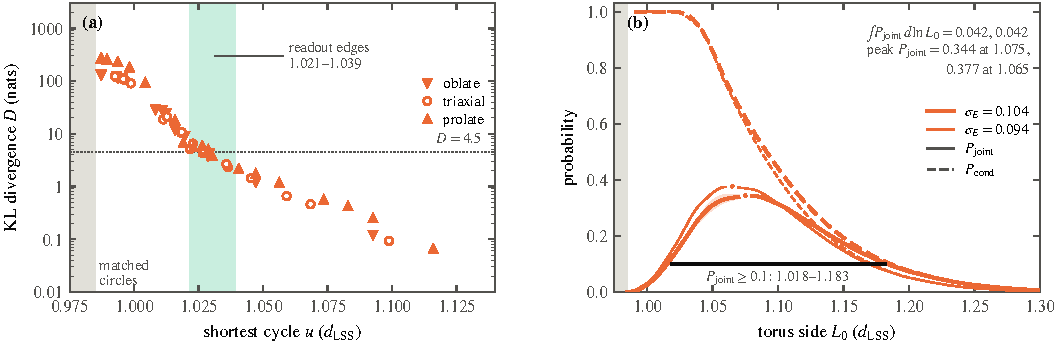
\includegraphics[width=\textwidth]{prd_fossil_sky}
\caption{Microwave-background readability of the shape fossil, set by the shortest cycle. (a)~Kullback--Leibler divergence of $55$ computed fossils from the closest circle-free cube, for temperature and $E$ modes with $2\leq\ell\leq80$ on the full sky, versus their shortest cycle $u$; band: readout edges of the 15 interpolated shapes; dotted: the readability criterion $D=4.5$; gray: excluded by matched circles. (b)~Probability that a predicted fossil is readable with no matched circles (solid) and given that circles are absent (dashed), versus the present size $L_0$, for $\sigma_E=0.104$ (thick; light band: edge-interpolation bounds) and $0.094$ (thin); bar: $P_{\rm joint}\geq0.1$. Below $L_0\simeq1.03\,\dLSS$ the dashed curve depends on the readout edge for $A<0.25$, where no fossil was computed; $P_{\rm cond}$ must vanish as $L_0\to0.985\,\dLSS$ (Sec.~\ref{rA:c-ens}).} %
\label{fig:rA-sky}
\end{figure}

\subsection{From the turning point to today}
\label{rA:c-today}

Once the Casimir force has switched off, nothing changes the shape.
Without a force the shape momenta $P_A=\MPbar^2L^3\dot\beta_A$ are conserved, so the shape velocity decays as $L^{-3}$ and the total further change of $\beta_A$, $\int P_A\,dt/\MPbar^2L^3$, converges; no homogeneous force acts on the moduli during inflation, reheating or the later expansion.
The fundamental domain today therefore has the frozen shape of Sec.~\ref{rA:s-fossil}, scaled to a present size $L_0$, which we define by its volume $L_0^3$.
Two of its properties follow from the Standard Model content and the $A_s$-calibrated plateau.
The aspect fossil is $\sigma_E=0.104$ per mode at leading order, $0.0934$ at next order and $0.059$ for free fields (Table~\ref{tab:rA-fossil}). %
The ratio $\sigma_{T_2}/\sigma_E=0.062$, or $0.11$ for free fields, keeps the edge angles sixteen (nine) times closer to $90^\circ$ than the aspect ratios are to unity. %
The size is not predicted: $L_0$ grows as $e^{N_{\rm post}}$, and $N_{\rm post}$ depends on where on the plateau the turning point sits (Sec.~\ref{rA:c-size}).

\subsection{The shortest cycle decides}
\label{rA:c-shortest}

A torus smaller than the last-scattering sphere produces pairs of matched circles~\cite{Cornish:1997ab}, and their absence requires every translation of the torus to exceed $0.985\,\dLSS$~\cite{Vaudrevange:2012da,COMPACT:2022nsu}. %
A somewhat larger torus still correlates harmonic coefficients of different $\ell$ and $m$~\cite{COMPACT:2023rkp,Himeno:2026lgh}, and these correlations carry its shape.
We computed the exact covariance of the temperature and $E$-mode coefficients for $2\leq\ell\leq80$ on the full sky, for $55$ deformed tori that cover the predicted shapes, and the Kullback--Leibler divergence $D$ of each from the circle-free cubic torus that is closest to it in this measure (Sec.~\ref{rA:c-cov}). %

\paragraph{Readability criterion.}
We call a fossil readable if $D\geq4.5$. %
For two Gaussian models of the data the expected log-likelihood ratio is $D$, so the expected $\Delta\chi^2$ is $2D$; for nested Gaussian models $2D=9$ corresponds to $3\sigma$ for a deformation of known direction, and the threshold is stricter than the $D\gtrsim3$ that Ref.~\cite{COMPACT:2022gbl} associates with a strong detection of topology. %

\paragraph{Parametrization of the fossil.}
The aspect part of the fossil lies in the $E$ plane,
\begin{equation}
\beta=A\,\sigma_E\big(\cos\theta\,X_d+\sin\theta\,X_{d2}\big),
\label{eq:rA-Eplane}
\end{equation}
with $A$ Rayleigh distributed (median $\sqrt{2\ln2}=1.177$, rms $\sqrt2$) and $\theta$ uniform for the Gaussian of Sec.~\ref{rA:s-fossil}, because the two aspect amplitudes are independent with equal widths. %
For diagonal $G=e^{2\beta}$ the sides are $L_i=L_0e^{\beta_{ii}}$, and Eq.~\eqref{eq:rA-XE} gives
\begin{equation}
\beta_{ii}=\sqrt{\tfrac23}\,A\sigma_E\cos(\theta-\theta_i),\qquad \theta_i=30^\circ,\ 150^\circ,\ 270^\circ,
\end{equation}
so the sides are $L_0\exp[\sqrt{2/3}\,A\sigma_E\cos(\theta-\theta_i)]$, and we write $u$ for the shortest of them.
The cubic group acts on this plane as the dihedral group of order six, generated by rotations by $120^\circ$, which permute the edges, and by reflections.
Its invariants are $\Tr\beta^2=A^2\sigma_E^2$ and $\Tr\beta^3=(2/3)^{3/2}\sum_i\cos^3(\theta-\theta_i)A^3\sigma_E^3=\tfrac34(2/3)^{3/2}A^3\sigma_E^3\sin3\theta$, so every observable depends on $\beta$ through $A^2$ and $A^3\sin3\theta$, and $-\pi/6\leq\theta\leq\pi/6$ covers all shapes.
At $\theta=\pi/6$ one side is long and two are short (prolate), at $\theta=-\pi/6$ two are long and one is short (oblate), and $\theta=0$ is triaxial.
The angle modes change $D$ only at second order, by about $0.4\%$ for $\sigma_{T_2}=0.0065$, and we neglect them (Sec.~\ref{rA:c-edges}). %

\paragraph{Result.}
We find that the divergence is a steep function of $u$ and depends on the amplitude and orientation of the fossil almost only through it [Fig.~\ref{fig:rA-sky}(a)].
Near the circle bound, $u\simeq0.99\,\dLSS$, it is $D\simeq90$--$270$ for every computed amplitude from $A=0.25$ to $2$; it falls to about $4.5$ at $u\simeq1.027\,\dLSS$, to $1$ at $1.05$ and to $0.1$ at $1.10\,\dLSS$. %
Over the $15$ computed shapes the readout edge $u_{\max}$, the shortest cycle at which $D=4.5$, lies between $1.021$ and $1.039\,\dLSS$, and between $1.023$ and $1.032\,\dLSS$ for $A\geq0.5$ (Table~\ref{tab:rA-edges}). %
A fit to all points with $0.2<D<80$ gives
\begin{equation}
\ln D=3.25+0.07\ln A-56\,(u/\dLSS-1)-0.05\sin3\theta
\end{equation}
with a scatter of $0.34$. %
What the maps resolve is set by how close the nearest image comes; the amplitude and orientation of the fossil decide mainly at which $L_0$ that happens.
Near the edge $\ln D$ falls by $85$--$130$ per unit of $u/\dLSS$, so doubling the information moves the edge outward by only about $0.008\,\dLSS$. %

\subsection{Covariance and divergence}
\label{rA:c-cov}

\paragraph{Covariance on the torus.}
For a torus with lattice basis $B=L_0G^{1/2}$ the allowed wave vectors are $\bm k_{\bm n}=2\pi B^{-\mathsf T}\bm n$.
The primordial curvature perturbation is a Fourier series, and the harmonic coefficients of the temperature and $E$ modes, $X\in\{T,E\}$, follow from it with the transfer functions $\Delta^X_\ell$:
\begin{equation}
\zeta(\bm x)=\sum_{\bm n}\zeta_{\bm n}e^{i\bm k_{\bm n}\cdot\bm x},\qquad \langle\zeta_{\bm n}\zeta^*_{\bm n'}\rangle=\frac{P_\zeta(k_{\bm n})}{L_0^3}\,\delta_{\bm n\bm n'},\qquad
a^X_{\ell m}=4\pi i^\ell\sum_{\bm n}\Delta^X_\ell(k_{\bm n})\,\zeta_{\bm n}\,Y^*_{\ell m}(\hat{\bm k}_{\bm n}).
\end{equation}
Their covariance is therefore~\cite{COMPACT:2023rkp}
\begin{equation}
C^{XY}_{\ell m,\ell'm'}=\frac{(4\pi)^2}{L_0^3}\,i^{\ell-\ell'}\sum_{\bm n\neq0}P_\zeta(k_{\bm n})\,\Delta^X_\ell(k_{\bm n})\Delta^Y_{\ell'}(k_{\bm n})\,Y_{\ell m}(\hat{\bm k}_{\bm n})\,Y_{\ell'm'}(\hat{\bm k}_{\bm n})
\label{eq:rA-cov}
\end{equation}
in a real harmonic basis; the zero mode $\bm n=0$ carries no fluctuation.
The transfer functions $\Delta^X_\ell$ of unlensed scalar perturbations are computed with CAMB~\cite{Lewis:1999bs} for the Planck 2018 $\Lambda$CDM parameters~\cite{Planck:2018vyg}.
CAMB sets $\Delta_\ell$ to zero below $k\chi_*\simeq14$ for $18\leq\ell\leq26$, and we continue it there with the spherical Bessel asymptotics, which matters for the few lowest torus modes. %
Modes with $k\chi_*>x_{\max}$ are replaced by the isotropic continuum through a smooth taper over the last quarter of that range, which makes $C$ a smooth function of the shape; for $\ell\leq80$ we use $x_{\max}=240$. %
At $L_0=6\,\dLSS$ the construction reproduces the covering-space spectra with $D\sim10^{-6}$. %

\paragraph{Block structure.}
For a diagonal $G$, which includes every shape of Eq.~\eqref{eq:rA-Eplane}, each coordinate reflection maps the lattice to itself and leaves $P_\zeta$, $\Delta_\ell$ and the taper invariant.
Under $x\to-x$ the azimuth goes to $\pi-\varphi$, so $\cos m\varphi$ picks up $(-1)^m$ and $\sin m\varphi$ picks up $(-1)^{m+1}$; under $y\to-y$, $\varphi\to-\varphi$ flips only the sine harmonics; and under $z\to-z$, $P^m_\ell$ picks up $(-1)^{\ell+m}$.
Real harmonics therefore carry the character $(|m|+[m<0],\,[m<0],\,\ell+|m|)$ mod $2$ under the three reflections, and sums over orbits of different characters vanish.
The covariance therefore splits exactly into eight blocks, and the divergence is the sum of the block divergences.
At a generic point of the $E$ plane, $(A,\theta)=(1.3,0.37)$, the whitened elements between different characters are below $1.6\times10^{-16}$, and the full-matrix divergence equals the sum over blocks to all printed digits. %

\paragraph{Divergence.}
The divergence of a fossil covariance $C_\beta$ from a reference $C_0$ is
\begin{equation}
D(C_\beta\|C_0)=\tfrac12\Big[\Tr\big(C_0^{-1}C_\beta\big)-n-\ln\det\big(C_0^{-1}C_\beta\big)\Big],
\label{eq:rA-kl}
\end{equation}
with $n$ the dimension, the expected log-likelihood ratio of the two zero-mean Gaussian models when the data follow $C_\beta$.
We evaluate it from traces and log-determinants of packed inverses to a relative accuracy of $1.7\times10^{-12}$. %
The fixed divergence uses the cube of equal volume.
The profiled divergence minimizes over the side $s'\geq0.985\,\dLSS$ of a circle-free cube aligned with the axes of the fossil, over a pool of $19$ cubes spaced by at most $0.015\,\dLSS$. %
A bracketed Brent search on three fossils at the edge finds interior minima $0.04$--$0.55\%$ below the pool minima, which moves the edges by at most $6\times10^{-5}\,\dLSS$. %
A three-point parabolic refinement undershoots where the profile rises steeply toward the circle bound, so we use the pool minima.
Profiling lowers the integrated measure, Eq.~\eqref{eq:rA-measure}, from $0.0442$ to $0.0422$, and a free overall amplitude of the spectrum is optimal at $1.0000$--$1.0006$ and changes nothing. %

\paragraph{Fisher matrix.}
At the cube the Fisher matrix
\begin{equation}
F_{AB}=\tfrac12\Tr\big(C^{-1}\partial_AC\,C^{-1}\partial_BC\big)
\label{eq:rA-fisher}
\end{equation}
is block diagonal in the $E$, $T_2$ and rotation ($T_1$) representations of the cubic group.
For $\ell\leq30$ the uncertainty of one aspect amplitude is $\sigma(\beta_E)=0.023$, $0.073$ and $0.25$ at $L_0=1.05$, $1.1$ and $1.2\,\dLSS$, and the angle fossil, $0.0065$ per mode, stays below its $1\sigma$ uncertainty at every size allowed for a typical fossil. %
Near the circle bound the quadratic Fisher estimate misjudges deformations of fossil size by factors between $0.2$ and $3$, which is why we use the exact divergence. %

\subsection{Fossils and readout edges}
\label{rA:c-edges}

We computed $55$ fossils with $A\in\{0.25,0.5,1,\sqrt2,2\}$ and $\theta\in\{-\pi/6,0,\pi/6\}$, each at two to six sizes with $u\simeq0.987$--$1.12\,\dLSS$, including slices at $L_0=1.13$, $1.14$ and $1.15\,\dLSS$, against the $19$ reference cubes. %
Table~\ref{tab:rA-edges} lists the readout edges.
For $A=0.25$ both computed sizes lie above the threshold, and the edge is extrapolated upward, with the last chord as lower bound and a shallow slope of $60$ per unit of $u/\dLSS$ as upper bound. %
For the other amplitudes the chord between the computed sizes bounds the edge from above and the extension of the steeper preceding segment from below.

\begin{table}[tbp]
\centering
\caption{Readout edge $u_{\max}/\dLSS$, the shortest cycle at which $D=4.5$, for temperature and $E$ modes with $\ell\leq80$ and the profiled reference cube, at amplitude $A$ of Eq.~\eqref{eq:rA-Eplane}. Ranges are convex bounds from the computed sizes; the row $A=0.25$ is extrapolated.}
\label{tab:rA-edges}
\begin{tabular}{lccc}
\toprule
$A$ & oblate & triaxial & prolate\\
\midrule
$0.25$ & $1.0282$--$1.0393$ & $1.0233$--$1.0350$ & $1.0214$--$1.0259$\\ %
$0.5$ & $1.0275$--$1.0322$ & $1.0229$--$1.0242$ & $1.0247$--$1.0275$\\ %
$1$ & $1.0271$ & $1.0262$ & $1.0287$\\ %
$\sqrt2$ & $1.0253$--$1.0279$ & $1.0263$--$1.0272$ & $1.0287$--$1.0302$\\ %
$2$ & $1.0289$ & $1.0279$--$1.0282$ & $1.0300$--$1.0308$\\ %
\bottomrule
\end{tabular}
\end{table}

\paragraph{No polynomial law in the window.}
At fixed $L_0$ the leading invariants allowed by the cubic symmetry far from the circle bound motivate a fit $D=c_2A^2+c_3A^3\sin3\theta+c_4A^4$.
In the window this fit fails: at $L_0=1.14\,\dLSS$ its relative residuals have an rms of $4.9$, and it predicts negative $D$ for prolate shapes. %
There the orientations differ by their shortest cycles, so the divergence of a single fossil and its dependence on $\ell_{\max}$ cannot be carried over to the ensemble by a polynomial in $A$.

\paragraph{Angle modes.}
On diagonal shapes each angle direction $X_{ij}$ is odd under two reflections and couples different characters, so the angle modes change $D$ only at second order.
For the typical fossil at $L_0=1.13\,\dLSS$ and $\ell\leq40$, an angle amplitude $0.0065$ along $X_{12}$ lowers $D$ by $0.12\%$, and twice that amplitude by $0.50\%$, a ratio of $3.996$, as expected for a quadratic effect. %
With the ratio $F_{T_2}/F_E=0.647$ at the cube, the expected angle contribution is about $0.4\%$ of the aspect one. %

\subsection{Readability over the predicted shapes}
\label{rA:c-ensemble}

At a given present size the fossil is readable if $0.985\,\dLSS\leq u\leq u_{\max}$. %
Averaging over the Gaussian distribution of Eq.~\eqref{eq:rA-Eplane} gives the joint probability $P_{\rm joint}(L_0)$ that the fossil is readable and matched circles are absent, and the conditional probability $P_{\rm cond}$ given that circles are absent [Fig.~\ref{fig:rA-sky}(b)].
For temperature and $E$ modes to $\ell=80$, $P_{\rm joint}$ peaks at $0.344$ near $L_0=1.075\,\dLSS$, with bounds $0.339$--$0.351$ from the interpolation of the readout edges, and it never reaches one half. %
It exceeds $0.3$ for $1.048<L_0/\dLSS<1.105$, $0.2$ for $1.033$--$1.140$ and $0.1$ for $1.018$--$1.183$. %
Given that circles are absent, the fossil is readable with probability above one half up to $L_0=1.090\,\dLSS$, and with probability $0.44$, $0.32$, $0.23$ and $0.16$ at $L_0=1.10$, $1.12$, $1.14$ and $1.16\,\dLSS$. %
Below about $1.03\,\dLSS$ the conditional probability rests on an extrapolation of the readout edge to amplitudes $A<0.25$, but there at most a fifth of the fossils are free of circles (Sec.~\ref{rA:c-ens}). %

\paragraph{The integrated measure.}
Averaging over shapes spreads the readable sizes without adding to them.
For a fixed shape $\ln u=\ln L_0+\min_i\beta_{ii}$, so the readable range of $\ln L_0$ is an interval of width $\ln(u_{\max}/0.985\,\dLSS)$, shifted by the shape; integrating $P_{\rm joint}$ over $\ln L_0$ and then averaging over shapes gives
\begin{equation}
\int P_{\rm joint}\,d\ln L_0=\Big\langle\ln\frac{u_{\max}}{0.985\,\dLSS}\Big\rangle=0.042,
\label{eq:rA-measure}
\end{equation} %
almost exactly the width, $0.0415$, of the window of a single typical fossil, $|\beta_E|=\sqrt2\,\sigma_E$ along $X_d$, which is readable for $1.093<L_0/\dLSS<1.139$. %
The distribution of shapes turns that window into a band with a peak probability of about one third, $3.6$ times wider in $\ln L_0$ at the $0.1$ level. %
Inside the window of the typical fossil the joint probability falls from about one third to one fifth, because there smaller fossils have their shortest cycle beyond the edge and larger ones have circles. %
At the peak, $L_0=1.075\,\dLSS$, the typical fossil itself has circles; the readable fossils there have $u$ between $0.985$ and about $1.027\,\dLSS$, with $A\simeq0.5$--$1.2$ for oblate and triaxial and $A\simeq1.0$--$2.1$ for prolate shapes. %

\paragraph{Next order.}
The next-order zero-mode corrections shrink the fossil to $\sigma_E=0.0934$ (Sec.~\ref{rA:s-fossil}). %
With $\sigma_E=0.094$ the peak rises to $0.377$ near $L_0=1.065\,\dLSS$ and the $0.1$ level spans $1.015$--$1.168\,\dLSS$. %
The integrated measure, $0.0421$, does not change, since Eq.~\eqref{eq:rA-measure} depends only on the readout edges. %
A $10\%$ smaller (larger) $\sigma_E$ raises (lowers) the peak by about $9$--$10\%$ and moves the upper end of the $0.1$ range by $-0.013$ ($+0.015$)\,$\dLSS$. %

\paragraph{Information used.}
The conclusion depends little on the information used.
From $\ell\leq30$ to $\ell\leq80$ the divergence of the typical fossil at $L_0=1.13\,\dLSS$ grows by a factor of about $2.2$. %
The peak probability, the integrated measure and the conditional probability at $1.10\,\dLSS$ grow only by factors $1.23$--$1.31$, because more information moves the readout edge only slightly. %
White noise and beams of the Planck $143$\,GHz type lower the peak to $0.313$ and the integrated measure by $9\%$; temperature alone gives $0.286$ and $0.035$ (Table~\ref{tab:rA-variants}). %
Masks, foregrounds and the uncertainty of the reionization optical depth, which dominates the lowest $E$ multipoles, are not included; they reduce the information and lower these probabilities further.

\begin{table}[tbp]
\centering
\caption{Readability over the predicted shapes: peak of $P_{\rm joint}$ with its position $L_0/\dLSS$, the range of $L_0/\dLSS$ with $P_{\rm joint}\geq0.1$, and the integrated measure, Eq.~\eqref{eq:rA-measure}. TE80 denotes temperature and $E$ modes with $\ell\leq80$, and so on; the reference cube is profiled except in the second row (equal volume). Noise is white with a Gaussian beam of the Planck $143$\,GHz type. All rows use $\sigma_E=0.1041$ except the last.}
\label{tab:rA-variants}
\begin{tabular}{lccc}
\toprule
Readout & $P_{\rm joint}^{\max}$ & $P_{\rm joint}\geq0.1$ & Measure\\
\midrule
TE80 & $0.344$ ($1.075$) & $1.018$--$1.183$ & $0.0422$\\ %
TE80, fixed & $0.360$ ($1.078$) & $1.018$--$1.185$ & $0.0442$\\ %
TE40 & $0.305$ ($1.075$) & $1.018$--$1.178$ & $0.0377$\\ %
TE30 & $0.264$ ($1.078$) & $1.020$--$1.168$ & $0.0325$\\ %
T80 & $0.286$ ($1.078$) & $1.018$--$1.173$ & $0.0352$\\ %
TE80, noise & $0.313$ ($1.075$) & $1.018$--$1.178$ & $0.0384$\\ %
TE30, noise & $0.190$ ($1.080$) & $1.035$--$1.150$ & $0.0228$\\ %
TE80, $\sigma_E=0.094$ & $0.377$ ($1.065$) & $1.015$--$1.168$ & $0.0421$\\ %
\bottomrule
\end{tabular}
\end{table}

\subsubsection{Ensemble method}
\label{rA:c-ens}

The ensemble uses $2\times10^6$ shapes drawn from Eq.~\eqref{eq:rA-Eplane} with $\sigma_E=0.1041$, which gives a binomial error below $3.4\times10^{-4}$. %
Within each $\theta$ the readout edge is interpolated piecewise linearly in $A$, extrapolated linearly below $A=0.25$ and held constant above $A=2$, and it is interpolated quadratically in $\sin3\theta$ through the three computed orientations; the grid in $L_0$ has steps of $0.0025\,\dLSS$. %
The convex bounds on the edges give the bounds $0.339$--$0.351$ on the peak of $P_{\rm joint}$. %
This ensemble is the predicted distribution, in which the two aspect amplitudes of a rectangular torus are independent with equal widths and the angle amplitudes are sixteen times narrower.
It differs from the eigenvalue law of an isotropic five-component deformation, which carries a Vandermonde factor $\propto A^3|\cos3\theta|$ and gives non-rectangular lattices. %
Table~\ref{tab:rA-variants} summarizes the readouts.

For $L_0\leq1.03\,\dLSS$ the conditional probability depends on the readout edge for $A<0.25$, where no fossil was computed.
At $L_0=1.00$ and $1.02\,\dLSS$ it is $0.956$ and $0.945$ for $D\propto A^2$, $1.00$ and $0.997$ for the linear extrapolation used in the ensemble, and $0.12$ and $0.76$ in the extreme case that such fossils are unreadable. %
It must vanish as $L_0\to0.985\,\dLSS$, where only fossils close to the cube, with $D\to0$, are free of circles.
The lower end of the range $P_{\rm cond}\geq1/2$ thus lies between $0.986$ and $1.009\,\dLSS$, while the upper ends, $1.090$, $1.1225$, $1.1475$ and $1.185\,\dLSS$ for $P_{\rm cond}\geq0.5$, $0.3$, $0.2$ and $0.1$, are robust. %
The joint probability is affected only below $L_0\simeq1.03\,\dLSS$, where it is at most $0.2$. %

\subsection{Checks}
\label{rA:c-checks}

Our covariance code reproduces the stored covariance matrices of an earlier single-fossil analysis (Sec.~\ref{rep:v-conditional}).
For the typical fossil at $L_0=1.13\,\dLSS$ and $x_{\max}=320$ it gives $D=11.3495$ for $\ell\leq80$, equal to the cached value to $2\times10^{-14}$, and a fresh build agrees with the cached matrix to $2\times10^{-16}$ after whitening. %
At the edge of the typical fossil, $L_0=1.14\,\dLSS$, raising $x_{\max}$ from $240$ to $320$ changes the profiled divergence for $\ell\leq80$ by $-0.69\%$, and halving the taper changes it by $+0.17\%$. %
This moves the edge by about $10^{-4}\,\dLSS$; the other edges lie in the same regime near the circle bound, but only this one was tested. %
An independent build with CAMB~2.0.5 reproduces the divergence of the typical fossil at $L_0=1.13\,\dLSS$ for $\ell\leq40$, $7.226$, to $0.10\%$. %
An independent implementation of the ensemble from the tabulated divergences gives a peak of $0.350$ near $L_0=1.076\,\dLSS$, $P_{\rm joint}\geq0.1$ for $1.016$--$1.184\,\dLSS$ and an integrated measure of $0.0421$. %
For $\ell\leq30$ a separate temperature-only code, with a sharp cutoff and its own transfer functions, harmonics and mode sums, reproduces the Fisher widths at the cube to $1\%$ at $L_0=1.1\,\dLSS$ and $7\%$ at $1.2\,\dLSS$, and the divergence between the cubic torus and the covering space to $1\%$ for $1\leq L_0/\dLSS\leq1.3$. %
The noise of Table~\ref{tab:rA-variants} is white, $33$ and $70\,\mu$K\,arcmin for temperature and polarization, with an isotropic Gaussian beam of $7.3'$ full width at half maximum, which preserves the block structure; masks would break it and are not included. %
Further convergence data are collected in Sec.~\ref{rep:v-convergence}.

\subsection{The size of the torus}
\label{rA:c-size}

The model fixes the width of the distribution of present sizes but not its center.

\paragraph{A family of turning points.}
Time symmetry about the turn, $\Theta$ of Sec.~\ref{rA:s-equivalent}, sets $\dot\phi=\dot\beta=0$ there in a classical history.
The constraint at the turn, $V(\phi_b)\Lb^4=\rANeff\rAgam$, then leaves a one-parameter family of turning points labeled by the inflaton value $\phi_b$.
As $\phi_b$ runs from $4.9$ to $6.3\,\MPbar$, the number of $e$-folds after the turn grows from $38$ to $125$ while $\Lb$ changes by $0.6\%$, and $A_s$ fixes $h$ at the pivot independently of $\phi_b$. %
The center $\phi_b$ therefore sets $N_{\rm post}-N_*$, that is $\ln L_0$.
Neither the constraint, nor time symmetry and the reality conditions of Sec.~\ref{rA:s-equivalent}, nor $A_s$ selects $\phi_b$, and the minimal-energy-variance rule, applied to the center, has no interior minimum and drives $\phi_b$ to infinity.
Since $dN_{\rm post}/d\phi_b=58/\MPbar$ there, landing in the window of the typical fossil, $0.0415$ $e$-fold wide, requires $\phi_b$ to within $0.0415/58=7\times10^{-4}\,\MPbar$. %

\paragraph{A lower bound on the width.}
The width, in contrast, has a lower bound.
To linear order $N_{\rm post}-\bar N=\mathcal A\,\delta\phi_b+\mathcal B\,\delta P_b$, where $P_b$ is the momentum of the inflaton zero mode at the turn and $[\phi_b,P_b]=i$.
Time reversal maps $Q=\mathcal A\phi_b+\mathcal BP_b$ to $\bar Q=\mathcal A\phi_b-\mathcal BP_b$, so in a $\Theta$-invariant state, pure or mixed, $Q$ and $\bar Q$ have the same distribution, while
\begin{equation}
[Q,\bar Q]=-\mathcal A\mathcal B[\phi_b,P_b]+\mathcal B\mathcal A[P_b,\phi_b]=-2i\mathcal A\mathcal B .
\end{equation}
The uncertainty relation $\rAVar\,Q\,\rAVar\,\bar Q\geq\tfrac14|\langle[Q,\bar Q]\rangle|^2$ with $\rAVar\,Q=\rAVar\,\bar Q$ then gives
\begin{equation}
\sigma_N^2\geq|\mathcal A\mathcal B|,
\label{eq:rA-sizebound}
\end{equation}
provided the other sectors are uncorrelated with $(\phi_b,P_b)$ at linear order; the bound does not require a Gaussian state.
At the reference turning point it gives $\sigma_N\geq0.935$ $e$-fold, $0.938$ in the window of the typical fossil, and about $0.0137\,N_{\rm post}$ in general. %
The time-symmetric Gaussian of minimal energy variance (Sec.~\ref{rA:s-equivalent}), applied to the inflaton zero mode, whose energy spread is dominated by the slope of the plateau, gives $\sigma_N=0.959$, $2.5\%$ above the bound. %

\paragraph{Measures on the center.}
Probabilities need a measure on $\phi_b$.
For an amplitude independent of $\phi_b$, the Liouville measure on the turning surface, the Klein--Gordon norm of the expanding branch, the Schr\"odinger norm on a slice of fixed volume and the inverse-potential norm of Ref.~\cite{Godet:2026gqw} all give $p(N_{\rm post})\simeq1.17/N_{\rm post}$ for $38\leq N_{\rm post}\leq125$, which cannot be normalized on the plateau. %
With a cutoff the probability of a readable fossil, given that circles are absent, falls from $1.4\times10^{-3}$ for $N_{\rm post}\leq100$ to $5\times10^{-5}$ for $N_{\rm post}\leq10^6$. %
The only dependence on $\phi_b$ in the equations of the torus itself is the WKB factor $e^{\pm2S_E}$ of the Casimir-forbidden region $L<\Lb$, with $S_E\simeq1.2\times10^4$, and its sign is set by the inner boundary data, not by time symmetry. %
The growing sign, which resembles the no-boundary weight, gives $6.1\%$, and the decaying sign at most $6\times10^{-19}$. %
A time-symmetric Gaussian state of minimal width gives at most $1.5\%$ wherever it is centered. %
These rates use the readout edges for $\ell\leq30$; the edges for $\ell\leq80$ raise them by about a factor $1.2$. %

\paragraph{Priors on the size.}
For any prior on $\ln L_0$ that is broad on the scale of the window, the probability $P_{\rm cond}$ of a readable fossil given that circles are absent is the prior density, normalized to the sizes without circles, times the integrated measure, Eq.~\eqref{eq:rA-measure}.
A Gaussian of width $0.95$ in $\ln L_0$ centered at $1.13\,\dLSS$, about the width $\sigma_N=0.959$ of the model's own state of minimal energy variance above, gives $P_{\rm cond}\approx3.3\%$. %
The width $1.909$ of the inflaton packet of Sec.~\ref{rep:v-conditional}, which is what the same rule gives when the slope of the plateau is neglected, yields about $1.7\%$, and a prior $\propto L_0^{-\alpha}$ reaches $P_{\rm cond}=1/2$ only for $\alpha\simeq17.6$. %
An exponential prior of the no-boundary type with slope $3.2\times10^{-4}$ gives $1.3\times10^{-5}$, and the flat measure above with $N_{\rm post}\leq10^3$ gives $2.3\times10^{-4}$. %
These priors are conditional experiments, not measures derived from a wave function.
The values above use the parabolic profiles; the pool minima raise them by $2.3\%$. %
Relative to the readout edges for $\ell\leq30$, which the rates of the previous paragraph use, the edges for $\ell\leq80$ raise the probability of a readable fossil under broad priors by about a factor $1.2$, for instance from $1.4\%$ to $1.7\%$ for the Gaussian of width $1.909$. %
A readable fossil therefore needs a prior on the size sharply concentrated near the circle bound, and the model provides none.

\subsection{Present searches and tests}
\label{rA:c-tests}

Present searches allow the window.
For a cubic torus the Planck 2013 likelihood requires $L>0.92\,\dLSS$~\cite{Planck:2013okc}, the Planck 2015 likelihood $L>0.97\,\dLSS$~\cite{Planck:2015gmu}, and the absence of matched circles $L>0.985\,\dLSS$~\cite{COMPACT:2022nsu}. %
A shortest cycle between $0.985$ and about $1.04\,\dLSS$ is therefore allowed by circle and likelihood searches, and it lies within the range $L\lesssim1.2\,\dLSS$ where off-diagonal correlations remain detectable in principle~\cite{COMPACT:2023rkp}; no published analysis has excluded it. %

If a torus is found with its shortest cycle in this window, its fundamental domain should be close to a rectangular box.
Its aspect amplitudes should be compatible with an isotropic Gaussian of width $0.104$ per mode ($0.094$ at next order), truncated at large elongation by the absence of circles, and its angles should lie within about a degree of $90^\circ$. %
Angle deviations above about $20^\circ$, which the multipoles $\ell\leq30$ alone detect at $3\sigma$ for $L_0=1.10\,\dLSS$, would exclude the natural state. %
A single sky is one draw from the predicted distribution.
For two independent Gaussian amplitudes of width $\sigma_E$ the score of $\ln\sigma_E$ is $\sum_i(\beta_i^2/\sigma_E^2-1)$, whose variance is $2$ per amplitude, so the Fisher information on $\ln\sigma_E$ from the two aspect amplitudes of one torus is $4$, and even a perfect measurement tests the predicted width only to about $50\%$. %
A null topology search out to a shortest cycle of about $1.05\,\dLSS$ would close the window.
The Casimir sector leaves no other trace: its contribution to $\Delta N_{\rm eff}$ is negligible, and the primordial spectra are those of the plateau (Sec.~\ref{rep:spectra}).


\clearpage
\part{Alternative derivations and validation}

\section{Full-dimensional checks of the reduced zero-mode model}\label{rep:v-fulldim}

The criterion of Secs.~\ref{rep:h-reduced}--\ref{rep:h-smmap} rests on a two-dimensional model of the Higgs zero mode, in which the Higgs radius $r$ and the length $s=|\bm w|$ of the hypercharge zero mode are dynamical and the nine SU(2) zero modes enter through a conditional Gaussian corrected by a fixed-$r$ diffusion Monte Carlo (DMC) shape term.
In this section we test that reduction against the full zero-mode problem with sixteen coordinates.
We find that, inside a gauge-invariant wall placed beyond the barrier, the full ground-state energy lies below the two-dimensional one at the same wall by $-0.0032(8)/L$ at $\lambda=-0.010$ and $-0.0034(9)/L$ at $\lambda=-0.013$, independently of the wall position and of $\lambda$ (it is $-0.0043(9)/L$ at $\lambda=0$). %
The reduction error is therefore a constant shift of the well.
Four independent estimates of the resulting change of the width give $\Gamma_{\rm full}/\Gamma_{\rm 2D}=0.92$--$1.03$. %
With the slopes of the final hazard this moves the critical top mass by $+0.0046$, $+0.0075$ and $+0.0115\GeV$ at $\Pone=0.9$, $0.5$ and $0.1$, with a one-sided envelope of $+0.012$, $+0.020$ and $+0.031\GeV$, which is the ``full-dimensional validation'' item of the error budget of Sec.~\ref{rep:h-budget}. %
The code and the archived outputs are in \texttt{higgs/05\_fulldim\_validation} of the code package~\cite{DNECv12code}; the derivation file is D123.

\subsection{The full zero-mode problem}\label{sec:v18-problem}

We use unit-mass coordinates $y=(\bm x,\bm w,\bm\phi)\in\mathbb R^9\times\mathbb R^3\times\mathbb R^4$: the constant SU(2) connections $x_i^a$ ($i$ spatial, $a$ adjoint), the constant hypercharge connections $w_i$, and the four real components of the Higgs zero mode, $\Phi=(\phi_0+i\phi_1,\phi_2+i\phi_3)/\sqrt2$, with $r=|\bm\phi|$ and $\Phi^\dagger\Phi=r^2/2$.
Lengths and energies are in units of the edge $L$ (Sec.~\ref{rep:setup}).
The Hamiltonian is
\begin{equation}
H=\tfrac12\,p^2+V(y),
\label{eq:v18-H}
\end{equation}
with
\begin{equation}
V(y)=g_2^2\,v_{\rm su2}(\bm x)+\sum_{i=1}^3\bigl|\bigl(g_2\,x_i^aT^a+g_Y\,Y\,w_i\bigr)\Phi\bigr|^2+\frac{\lambda}{4}\,r^4+\Delta V_{\rm MC}(r),
\label{eq:v18-V}
\end{equation}
where $T^a=\sigma^a/2$, $Y=1/2$, and
\begin{equation}
v_{\rm su2}(\bm x)=\frac14\sum_{i,j=1}^{3}\bigl|\bm x_i\times\bm x_j\bigr|^2
\label{eq:v18-vsu2}
\end{equation}
is the magnetic energy of constant SU(2) connections, $\bm x_i$ being the adjoint three-vector of direction $i$.
The last term of Eq.~(\ref{eq:v18-V}) is the one-loop matching of the non-zero modes of Sec.~\ref{rep:h-matching} (Coulomb gauge with the $\MSbar$ finite-volume sums), which depends on $r$ only; we evaluate it on $0\le r\le r_w$ with step $0.002$ and interpolate with a cubic spline.
All numbers in this section use the one-loop couplings of the zero-mode calculation of Sec.~\ref{rep:zeromodes}, $g_2=0.5268$, $g_Y=0.4415$ and $y_t=0.4585$, the second-stage model without the cross terms of Sec.~\ref{rep:h-cross}, and the full width $\Gamma=-2\,{\rm Im}\,E$ in units of $1/L$. %

For $\lambda<0$ the potential is unbounded from below along $r$, and the Hamiltonian~(\ref{eq:v18-H}) has no ground state; the resonance of Sec.~\ref{rep:h-reduced} is a Siegert state.
To obtain a ground-state problem that DMC can solve we impose a Dirichlet wall at $|\bm\phi|=r_w$.
Three properties make this wall harmless.
\begin{enumerate}
\item Constant SU(2)$\times$U(1)$_Y$ transformations act on $(\bm x,\bm w,\bm\phi)$ by orthogonal matrices and preserve $|\bm\phi|$, so both the wall and $H$ are gauge invariant.
\item The region $\{|\bm\phi|<r_w\}\times\mathbb R^{12}$ is connected and the Dirichlet semigroup $e^{-tH}$ is positivity improving on it.
The ground state is therefore unique and positive, hence invariant under every symmetry of $H$; in particular it is gauge invariant and satisfies Gauss's law without a projection.
\item The wall is the only node of the ground state, and it is exact.
DMC with a guiding function that vanishes on the wall therefore has no fixed-node error.
\end{enumerate}
Inside the wall the quartic term is bounded, $|\lambda| r^4/4\le|\lambda| r_w^4/4$, and the walled ground state exists.

\subsection{Placement of the walls}\label{sec:v18-walls}

We place the walls with the lowest adiabatic channel of the two-dimensional model,
\begin{equation}
U_{\rm ad}(r)=U_1(r)+\tfrac32\,\Omega_{\rm eff}(r),
\label{eq:v18-Uad}
\end{equation}
where $U_1$ is the $r$-dependent part of the two-dimensional Hamiltonian and $\Omega_{\rm eff}$ the stiffness of $\bm w$ (Sec.~\ref{rep:h-reduced}).
Let $r_1$ and $r_2$ be the inner and outer classical turning points at the resonance energy $\varepsilon$ and $r_{\rm top}$ the position of the barrier top.
A wall with $r_{\rm top}<r_w<r_2$ leaves no classically allowed region below $\varepsilon$ outside the barrier, so the lowest walled state is the state localized in the well.
Table~\ref{tab:v18-walls} lists the geometry and the walls.
Two further walls inside the barrier top serve only the tail estimate of Sec.~\ref{sec:v18-tail}.

\begin{table}[t]
\centering
\caption{Geometry of the lowest adiabatic channel~(\ref{eq:v18-Uad}) and positions of the walls (units of $L$). $U_{\rm ad}(r_w)-\varepsilon$ is given for the three main walls. Two inner walls, used only for the tail estimate, lie at $4.08$ and $4.32$ ($\lambda=-0.010$) and at $3.84$ and $4.08$ ($\lambda=-0.013$).}
\label{tab:v18-walls}
\begin{tabular}{ccccccc}
\toprule
$\lambda$ & $r_1$ & $r_{\rm top}$ & $U_{\rm top}$ & $r_2$ & main walls $r_w$ & $U_{\rm ad}(r_w)-\varepsilon$ \\
\midrule
$-0.010$ & $2.498$ & $4.344$ & $5.002$ & $5.737$ & $4.80,\ 5.12,\ 5.44$ & $0.64,\ 0.51,\ 0.26$ \\ %
$-0.013$ & $2.510$ & $4.022$ & $4.812$ & $5.188$ & $4.40,\ 4.64,\ 4.96$ & $0.48,\ 0.38,\ 0.17$ \\ %
\bottomrule
\end{tabular}
\end{table}

\begin{figure}[t]
\centering
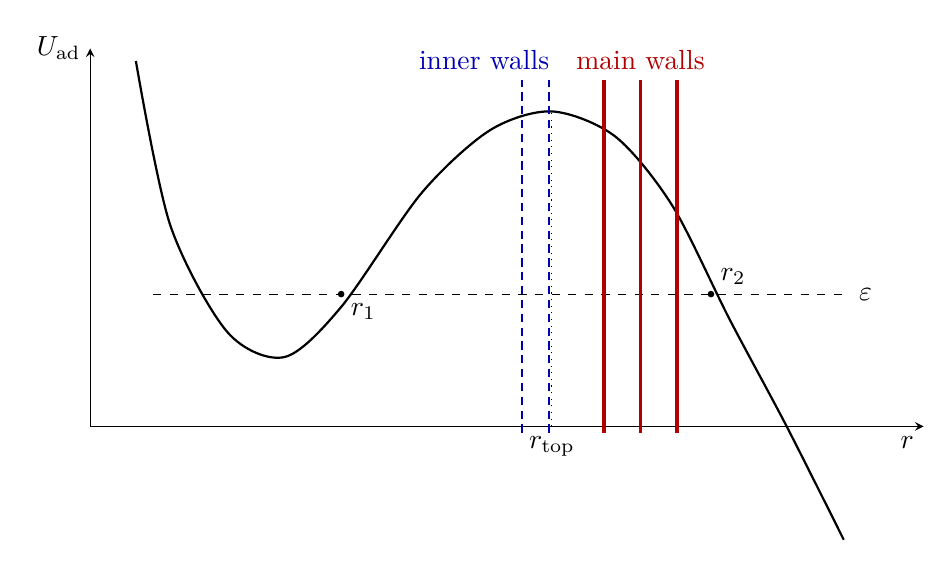
\begin{tikzpicture}[x=1.45cm,y=1.6cm,>=stealth]
\draw[->] (0.3,0) -- (7.6,0) node[below left]{$r$};
\draw[->] (0.3,0) -- (0.3,3.0) node[left]{$U_{\rm ad}$};
\draw[thick,smooth] plot coordinates {(0.7,2.9) (1.0,1.6) (1.5,0.75) (2.0,0.55) (2.5,0.95) (3.2,1.85) (3.8,2.35) (4.344,2.5) (4.9,2.3) (5.4,1.75) (5.9,0.85) (6.4,0.0) (6.9,-0.9)};
\draw[dashed] (0.85,1.05) -- (6.95,1.05) node[right]{$\varepsilon$};
\fill (2.498,1.05) circle (1.2pt) node[below right]{$r_1$};
\fill (5.737,1.05) circle (1.2pt) node[above right]{$r_2$};
\draw[dotted] (4.344,0) -- (4.344,2.5);
\node[below] at (4.344,0) {$r_{\rm top}$};
\foreach \x in {4.80,5.12,5.44} \draw[very thick,red!70!black] (\x,-0.05) -- (\x,2.75);
\foreach \x in {4.08,4.32} \draw[thick,blue!70!black,densely dashed] (\x,-0.05) -- (\x,2.75);
\node[red!70!black,above] at (5.12,2.75) {main walls};
\node[blue!70!black,above] at (3.75,2.75) {inner walls};
\end{tikzpicture}
\caption{Schematic of the walled problem at $\lambda=-0.010$ (not to scale). The main walls (solid) lie between the barrier top $r_{\rm top}=4.344$ and the outer turning point $r_2=5.737$ of the lowest adiabatic channel, so the lowest walled state is the well state; the inner walls (dashed), inside the barrier top, shift the energy by an amount set by the tunnelling tail and are used only for the tail-amplitude estimate of Sec.~\ref{sec:v18-tail}.}
\label{fig:v18-walls}
\end{figure}

\subsection{Diffusion Monte Carlo inside the wall}\label{sec:v18-dmc}

DMC projects the ground state by evolving in imaginary time.
For a guiding function $\psi_T$ and the mixed density $f(y,t)=\psi_T(y)\,\psi(y,t)$ the imaginary-time Schr\"odinger equation $-\partial_t\psi=(H-E_{\rm ref})\psi$ becomes
\begin{equation}
-\partial_t f=-\tfrac12\nabla^2f+\nabla\cdot\bigl(f\,\bm v\bigr)+\bigl[E_L(y)-E_{\rm ref}\bigr]f,
\qquad
\bm v=\nabla\ln\psi_T,\qquad E_L=\frac{H\psi_T}{\psi_T},
\label{eq:v18-fp}
\end{equation}
a drift--diffusion equation with branching~\cite{Foulkes:2001zz,Kosztin:1996fh}.
As $t\to\infty$, $f\to\psi_T\psi_0$, and the mixed estimator
\begin{equation}
E_{\rm mix}=\frac{\int f\,E_L\,dy}{\int f\,dy}=\frac{\langle\psi_0|H|\psi_T\rangle}{\langle\psi_0|\psi_T\rangle}=E_0
\label{eq:v18-mixed}
\end{equation}
is exact, because $H$ is Hermitian on functions that vanish on the wall and $\psi_0$ and $\psi_T$ obey the same Dirichlet condition.

\paragraph{Guiding function.}
We use
\begin{equation}
\psi_T(y)=\exp\!\Bigl(-\tfrac12a_x|\bm x|^2-\tfrac12a_w|\bm w|^2\Bigr)\,f_r(r),
\label{eq:v18-psiT}
\end{equation}
with $(a_x,a_w)$ from the optimal Gaussian at $\lambda=0$ of the zero-mode calculation and $f_r$ the ground state of the radial problem
\begin{equation}
-\frac12\Bigl(f_r''+\frac3r\,f_r'\Bigr)+U_g(r)\,f_r=\epsilon\,f_r,\qquad f_r(r_w)=0,
\label{eq:v18-radial}
\end{equation}
where $U_g=\frac\lambda4r^4+\Delta V_{\rm MC}+C_0+B_x+\delta E_{\rm DMC}+\frac32\Omega_{\rm eff}$ is the lowest adiabatic channel of the two-dimensional model without the Born--Huang term $B_w$ (Sec.~\ref{rep:h-reduced}); the factor $3/r$ is the radial Laplacian of the four Higgs components.
We solve Eq.~(\ref{eq:v18-radial}) by finite differences with step $0.001$ and interpolate $f_r$ by a cubic spline with $f_r'(0)=0$.
The local energy follows directly from the spline,
\begin{equation}
E_L(y)=\frac12\sum_ia_i-\frac12\sum_ia_i^2y_i^2-\frac{f_r''+3f_r'/r}{2f_r}+V(y),
\label{eq:v18-EL}
\end{equation}
where the sums run over the twelve gauge coordinates with $a_i=a_x$ or $a_w$; it is evaluated from the same spline that drives the walkers, so the drift, the Metropolis ratio and $E_L$ are consistent.

\paragraph{Moves and population.}
Each walker moves by the short-time Green function $y'=y+\bar{\bm v}\,\tau+\sqrt\tau\,\bm\eta$, $\bm\eta$ a standard normal vector, and the move is accepted with the Reynolds--Umrigar Metropolis probability that restores detailed balance for $\psi_T^2$~\cite{Umrigar:1993dmc}.
On the four Higgs components the drift is limited as
\begin{equation}
\bar{\bm v}=\frac{-1+\sqrt{1+2a\,v^2\tau}}{a\,v^2\tau}\;\bm v,\qquad a=0.5,
\label{eq:v18-drift}
\end{equation}
which leaves small drifts unchanged and caps the drift near the node at the wall; the same formula is used in the forward and the reverse Green function. %
Every proposal with $r'\ge r_w$ is rejected, since $\psi_T=0$ there; at most $2\times10^{-6}$ of the moves are rejected for this reason. %
Branching uses the effective time step $\tau_{\rm eff}=\tau\times(\text{acceptance ratio})$, the population is fixed at $W=10^4$ walkers by systematic resampling, and $E_{\rm ref}$ is adjusted slowly. %

\paragraph{Statistics and time step.}
For every wall and every time step we run two independent shards, each with equilibration time $10$ and production time $40$.
The seed of a shard is fixed by the SHA-256 hash of the string \texttt{T14a|name|tau|k} and recorded in its output, so that each shard can be rerun bit for bit (the package rerun of one shard is identical).
Errors are block averages, the largest over block lengths $1$, $2$ and $4$; shards are combined with inverse-variance weights and the error is inflated when their scatter exceeds it.
We extrapolate linearly in $\tau_{\rm eff}$ from $\tau=0.04$, $0.02$ and $0.01$; the fitted slopes are $0.02$--$0.15$ with $\chi^2\le1.6$ for one degree of freedom, and the extrapolated energy differs from the smallest-step value by at most $0.002$, which is contained in the extrapolation error. %
After extrapolation the statistical error of a single wall is $0.0010$--$0.0025$. %
In total the calculation uses $66$ shards (eleven walled cases, three time steps, two shards each).

\subsection{The two-dimensional model at the same wall}\label{sec:v18-2d}

The comparison must use the same wall in both models, because a wall below the barrier top shifts the two-dimensional energy by up to $0.024$, far more than the effect we look for.
We discretize the two-dimensional Hamiltonian of Sec.~\ref{rep:h-reduced} (both the model with the DMC shape correction, 2D, and its Gaussian version, 2D$_{\rm G}$) with second-order finite differences in $r$ and $s$, with Dirichlet conditions at $r=r_w$ and $s=12$, at steps $h=0.08$, $0.04$ and $0.02$.
For an energy $E(h)=E+c_2h^2+c_4h^4+O(h^6)$ the two Richardson steps
\begin{equation}
E^{(2)}(h)=\frac{4E(h/2)-E(h)}{3},\qquad E^{(4)}=\frac{16E^{(2)}(h/2)-E^{(2)}(h)}{15}
\label{eq:v18-richardson}
\end{equation}
remove the $h^2$ and $h^4$ terms; $E^{(2)}$ and $E^{(4)}$ differ by at most $2\times10^{-6}$. %
At $\lambda=0$ the code reproduces the finite-difference values $4.450855$ (2D) and $4.507693$ (2D$_{\rm G}$) of the reduced-model calculation, which the Numerov solver of Sec.~\ref{rep:h-reduced} gives as $4.450863$. %
A $\pm1\sigma$ tilt of the DMC shape correction $\delta E_{\rm DMC}$ changes the two-dimensional energy by $\pm0.0025$ at $\lambda=0$ and $\pm0.0022$ at the middle walls for $\lambda<0$. %
The full DMC contains no such correction, so the difference $\Delta\varepsilon=\varepsilon_{\rm full}-\varepsilon_{\rm 2D}$ measures the reduction error relative to the central two-dimensional model.

\subsection{Results}\label{sec:v18-results}

\paragraph{The benchmark at $\lambda=0$.}
Table~\ref{tab:v18-lam0} compares the reductions of the zero-mode problem with the full-dimensional DMC value at $\lambda=0$, $4.4478(13)$, without the matching term. %
The two-dimensional model is the only reduction within $0.004$ of the full value; the one-dimensional Gaussian reduction is $0.151$ too high, and the two Born--Oppenheimer bounds bracket the full value at $-0.014$ and $+0.098$.

\begin{table}[t]
\centering
\caption{Ground-state energy at $\lambda=0$ (units of $1/L$; local model without the matching term) for the reductions of Sec.~\ref{rep:h-reduced}, compared with full-dimensional DMC, $4.4478(13)$.}
\label{tab:v18-lam0}
\begin{tabular}{lcc}
\toprule
Reduction & $L\varepsilon_0$ & Difference \\
\midrule
One-dimensional, Gaussian (with $B_r$) & $4.5985$ & $+0.151$ \\ %
One-dimensional, exact gauge shape & $4.5434$ & $+0.096$ \\ %
Born--Oppenheimer bound, with $B_w$ & $4.5462$ & $+0.098$ \\ %
Born--Oppenheimer bound, without $B_w$ & $4.4334$ & $-0.014$ \\ %
Two-dimensional, Gaussian (2D$_{\rm G}$) & $4.5077$ & $+0.060$ \\ %
Two-dimensional (2D) & $4.4509$ & $+0.0031$ \\ %
\quad without $B_x$ & $4.4456$ & $-0.0022$ \\ %
\bottomrule
\end{tabular}
\end{table}

The walled code of this section, with the wall at $r_w=9$ where it has no effect, gives
\begin{equation}
\varepsilon_{\rm full}(\lambda=0)=4.44659(94),
\label{eq:v18-lam0}
\end{equation}
with a time-step slope of $0.083$ and $\chi^2=0.14$ for one degree of freedom. %
The unwalled code of the zero-mode calculation gives $4.44781(132)$; the difference is $-0.0012(16)$, or $0.75\sigma$, and the combined value is $4.44700(77)$. %
Against the two-dimensional model at the same wall ($r_w=8.96$), $\Delta\varepsilon(\lambda=0)=-0.0043(9)$, or $-0.0039(8)$ with the combined value; against 2D$_{\rm G}$ it is $-0.0611$. %

\paragraph{Negative quartic coupling.}
Tables~\ref{tab:v18-m010} and~\ref{tab:v18-m013} give the energies at every wall.
The Siegert resonance of the two-dimensional model lies at $\varepsilon_{\rm 2D}=4.286744$ with $\Gamma_{\rm 2D}=4.1535\times10^{-4}$ for $\lambda=-0.010$, and at $4.277899$ with $\Gamma_{\rm 2D}=2.2162\times10^{-3}$ for $\lambda=-0.013$; the column ``2D wall shift'' is the difference between the walled two-dimensional energy and this Siegert value. %

\begin{table}[t]
\centering
\caption{Walled energies at $\lambda=-0.010$ (units of $1/L$): full-dimensional DMC (extrapolated to zero time step), the two-dimensional model 2D and its Gaussian version 2D$_{\rm G}$ at the same wall (finite differences with Richardson extrapolation), their difference $\Delta\varepsilon=\varepsilon_{\rm full}-\varepsilon_{\rm 2D}$, and the shift of the 2D energy by the wall. The first two walls lie inside the barrier top.}
\label{tab:v18-m010}
\begin{tabular}{cccccc}
\toprule
$r_w$ & $\varepsilon_{\rm full}$ & $\varepsilon_{\rm 2D}$ & $\Delta\varepsilon$ & $\varepsilon_{\rm 2D_G}$ & 2D wall shift \\
\midrule
$4.08$ & $4.29394(145)$ & $4.298235$ & $-0.0043(15)$ & $4.352733$ & $+0.0115$ \\ %
$4.32$ & $4.29005(96)$ & $4.293356$ & $-0.0033(10)$ & $4.347474$ & $+0.0066$ \\ %
$4.80$ & $4.28584(103)$ & $4.288989$ & $-0.0031(10)$ & $4.342681$ & $+0.0022$ \\ %
$5.12$ & $4.28451(145)$ & $4.287887$ & $-0.0034(14)$ & $4.341440$ & $+0.0011$ \\ %
$5.44$ & $4.28411(203)$ & $4.287352$ & $-0.0032(20)$ & $4.340824$ & $+0.0006$ \\ %
\bottomrule
\end{tabular}
\end{table}

\begin{table}[t]
\centering
\caption{As Table~\ref{tab:v18-m010}, at $\lambda=-0.013$. The first two walls lie inside the barrier top.}
\label{tab:v18-m013}
\begin{tabular}{cccccc}
\toprule
$r_w$ & $\varepsilon_{\rm full}$ & $\varepsilon_{\rm 2D}$ & $\Delta\varepsilon$ & $\varepsilon_{\rm 2D_G}$ & 2D wall shift \\
\midrule
$3.84$ & $4.29921(117)$ & $4.302053$ & $-0.0028(12)$ & $4.356919$ & $+0.0242$ \\ %
$4.08$ & $4.29064(105)$ & $4.292774$ & $-0.0021(10)$ & $4.347034$ & $+0.0149$ \\ %
$4.40$ & $4.28018(252)$ & $4.285813$ & $-0.0056(25)$ & $4.339513$ & $+0.0079$ \\ %
$4.64$ & $4.27915(144)$ & $4.282919$ & $-0.0038(14)$ & $4.336333$ & $+0.0050$ \\ %
$4.96$ & $4.27798(118)$ & $4.280700$ & $-0.0027(12)$ & $4.333852$ & $+0.0028$ \\ %
\bottomrule
\end{tabular}
\end{table}

The inverse-variance means over the three main walls are
\begin{equation}
\Delta\varepsilon(-0.010)=-0.00323(78),\qquad \Delta\varepsilon(-0.013)=-0.00343(86),
\label{eq:v18-dE}
\end{equation}
with $\chi^2=0.02$ and $1.2$ for two degrees of freedom. %
Three facts follow from the tables.
First, $\Delta\varepsilon$ does not depend on the wall, although the two-dimensional wall shift itself varies from $0.0006$ to $0.008$ over the main walls and up to $0.024$ over all walls; the effect of the wall cancels in the difference.
The inner walls agree within errors (at $\lambda=-0.013$ the innermost two are slightly smaller, $-0.0028(12)$ and $-0.0021(10)$), and there is no trend with $r_w$.
Second, $\Delta\varepsilon$ does not depend on $\lambda$: $-0.0043(9)$, $-0.0032(8)$ and $-0.0034(9)$ at $\lambda=0$, $-0.010$ and $-0.013$.
The reduction error is a constant shift of about $-0.0035/L$ of the well.
Third, $\varepsilon_{\rm full}<\varepsilon_{\rm 2D_G}$ by $0.057$ at both negative couplings, so the variational bound of the Gaussian model, an upper bound for the trial family of Sec.~\ref{rep:h-reduced}, holds with the wall as well. %
The target $|\Delta\varepsilon|\le0.005$ set before the calculation is met at the central values; the $2\sigma$ upper limits are $0.0048$ and $0.0051$. %

\subsection{From the energy shift to the width: four estimates}\label{sec:v18-gamma}

A shift of the well changes the width through the energy at which the particle meets the barrier.
If the barrier is unchanged,
\begin{equation}
\rho\equiv\frac{\Gamma_{\rm full}}{\Gamma_{\rm 2D}}=\exp\!\Bigl(\Delta\varepsilon\,\frac{d\ln\Gamma}{d\varepsilon}\Bigr),
\label{eq:v18-rho}
\end{equation}
where $d\ln\Gamma/d\varepsilon$ is the response of the two-dimensional width to a shift of the well alone.
We test the assumption of an unchanged barrier with three further estimates that do not use Eq.~(\ref{eq:v18-rho}).
Table~\ref{tab:v18-four} collects the four ratios.

\paragraph{(i) Conversion with the well response.}
We add $\delta\,S(r)$ with $\delta=\pm0.006$ to the two-dimensional potential, where $S(r)=1$ for $r<1.8$ and falls to zero at $r=2.4$ as a squared cosine (profile A), or falls from $1.2$ to $2.4$ (profile B); both act only inside the inner turning point $r_1\approx2.5$. %
We compute the width with finite differences ($h=0.04$, $r\le11$, $s\le12$) and the complex absorbing potential $-i\eta(r-7)^2\theta(r-7)$, with $\eta$ at the most stable point of the Riss--Meyer criterion and held fixed for the shifted operators~\cite{Riss:1993cap}.
The two profiles give $d\ln\Gamma/d\varepsilon=7.43$ and $7.78$ at $\lambda=-0.010$ and $6.94$ and $7.29$ at $-0.013$; the curvature of $\ln\Gamma$ in $\varepsilon$ is below $0.1\%$. %
We take the mean and half the spread,
\begin{equation}
\frac{d\ln\Gamma}{d\varepsilon}=7.60(18)\ \ (\lambda=-0.010),\qquad 7.12(18)\ \ (\lambda=-0.013),
\label{eq:v18-dlng}
\end{equation}
so that Eq.~(\ref{eq:v18-rho}) gives $\ln\rho=(-0.00323)(7.60)=-0.0245(59)$ and $(-0.00343)(7.12)=-0.0244(61)$, that is, $\rho=0.976(6)$ at both couplings. %

\paragraph{(ii) Multidimensional adiabatic WKB.}
The most probable escape path runs along $r$.
We hold the transverse modes (SU(2), hypercharge and the Higgs angles) in their exact ground state at fixed $r$, whose energy is the body-frame DMC value $E^{\rm ex}_{\rm tot}(r)$ used for $\delta E_{\rm DMC}$.
Because the transverse equilibrium stays at the origin as $r$ changes, there is no corner-cutting correction at first order, and only the Born--Huang term remains.
The Gamow width is
\begin{equation}
\Gamma_{\rm WKB}=\frac{e^{-S}}{T_{\rm cl}},\qquad S=2\int_{r_1}^{r_2}\!dr\,\sqrt{2\,[U(r)-E]},
\label{eq:v18-gamow}
\end{equation}
with $T_{\rm cl}$ the classical period in the well.
For the two-dimensional model $U_{\rm 2D}=U_1+\frac32\Omega_{\rm eff}$ and $E=\varepsilon_{\rm 2D}$; for the full problem
\begin{equation}
U_{\rm full}=\frac{3}{8r^2}+\frac\lambda4r^4+\Delta V_{\rm MC}+E^{\rm ex}_{\rm tot}+B_r^{\rm G},\qquad E=\varepsilon_{\rm 2D}+\Delta\varepsilon,
\label{eq:v18-Ufull}
\end{equation}
where $B_r^{\rm G}$ is the Gaussian Born--Huang term of the radial motion.
Under the barrier $U_{\rm full}-U_{\rm 2D}=B_w+O(\beta'^4)\le0.005$: the two barriers coincide up to $B_w$. %
The result, $\rho=0.937$ at both couplings, factorizes into $0.973$ from $\Delta\varepsilon$ and $0.963$ from $B_w$ under the barrier. %
The WKB width itself is calibrated against the exact two-dimensional width: $\Gamma_{\rm WKB}/\Gamma_{\rm 2D}=1.059$ and $1.073$. %
Its slope $-dS/dE=8.71$ and $8.29$ is about $15\%$ larger than $d\ln\Gamma/d\varepsilon$ of Eq.~(\ref{eq:v18-dlng}), because a shift of the well also changes the normalization in the well, which enters the prefactor. %
Since $B_w$ is the spurious adiabatic term of the reduction (Sec.~\ref{rep:h-reduced}), we treat $0.937$ as the lower end of the range, not as the central value.

\paragraph{(iii) Amplitude of the tunnelling tail.}\label{sec:v18-tail}
This estimate uses only the full-dimensional data.
In WKB the well state has the amplitude $N$ at the inner turning point and decays under the barrier as $\exp(-\int_{r_1}^{r}\kappa\,dr')$, $\kappa=\{2[U(r)-E]\}^{1/2}$.
A Dirichlet wall at $r_w$ inside the barrier forces the tail to vanish and raises the energy by
\begin{equation}
\varepsilon(r_w)-\varepsilon_\infty\simeq N^2\exp\!\Bigl(-2\int_{r_1}^{r_w}\kappa\,dr\Bigr),
\label{eq:v18-wallshift}
\end{equation}
while the width is $\Gamma\simeq c\,N^2\exp(-2\int_{r_1}^{r_2}\kappa\,dr)$ with the same $N$.
If the two models have the same barrier, the ratio of their wall shifts at the same $r_w$ is
\begin{equation}
A\equiv\frac{\varepsilon_{\rm full}(r_w)-\varepsilon_{\rm full,\infty}}{\varepsilon_{\rm 2D}(r_w)-\varepsilon_{\rm 2D,\infty}}=\frac{N_{\rm full}^2}{N_{\rm 2D}^2}=\frac{\Gamma_{\rm full}}{\Gamma_{\rm 2D}}\,\exp\!\Bigl(2\Delta\varepsilon\int_{r_w}^{r_2}\frac{dr}{\kappa}\Bigr),
\label{eq:v18-A}
\end{equation}
where the last factor accounts for the shift of the turning point, $d\kappa/dE=-1/\kappa$; for $|\Delta\varepsilon|\approx0.003$ it is about $0.99$. %
A weighted linear fit of $\varepsilon_{\rm full}(r_w)=\varepsilon_\infty+A\,\delta\varepsilon_{\rm 2D}(r_w)$ over all five walls gives
\begin{equation}
A=0.92(16)\ \ (\lambda=-0.010),\qquad A=1.03(7)\ \ (\lambda=-0.013),
\label{eq:v18-Afit}
\end{equation}
and the extrapolated $\varepsilon_\infty-\varepsilon_{\rm 2D}=-0.0030(9)$ and $-0.0033(10)$, in agreement with Eq.~(\ref{eq:v18-dE}). %
This tests the barrier directly, to $16\%$ and $7\%$ at one standard deviation; the statistical error corresponds to about $\pm0.04\GeV$ in $m_c$. %

\paragraph{(iv) A collective coordinate for the SU(2) width.}
The conditional Gaussian of the SU(2) modes is optimized at every $r$; if its overall width could not follow the tunnelling, the reduction would miss a non-adiabatic effect.
We add the width scale $\zeta=e^{-q/2}$, $q=\ln[a/a_*(r)]$, as a third coordinate: the precisions $(a_*,a_*,k_*)$ become $(a_*,a_*,k_*)\,e^{q}$, the mean $-\beta_*\bm w$ is unchanged, and $\zeta=1$ is the pointwise optimum.
Because all Gaussian moments are known in closed form (Sec.~\ref{rep:h-reduced}), rescaling $a,k\to\zeta^{-2}a,\zeta^{-2}k$ term by term gives
\begin{align}
C_0(\zeta)={}&C_0+\tfrac34\bigl(2a+k+k\beta^2\bigr)\bigl(\zeta^{-2}-1\bigr)+\tfrac{3}{16}r^2\Bigl(\frac{2g_2^2}{a}+\frac{g_2^2}{k}\Bigr)\bigl(\zeta^{2}-1\bigr)\nonumber\\
&+\Bigl(\frac{3g_2^2}{4a^2}+\frac{3g_2^2}{2ak}\Bigr)\bigl(\zeta^{4}-1\bigr),\label{eq:v18-C0zeta}\\
\Omega_{\rm eff}^2(\zeta)={}&\Omega_{\rm eff}^2+\frac{2g_2^2\beta^2}{a}\bigl(\zeta^2-1\bigr)+\Bigl(\frac{4a\beta^2}{r^2}+\frac{k\beta'^2}{2}\Bigr)\bigl(\zeta^{-2}-1\bigr),
\label{eq:v18-Omzeta}
\end{align}
where kinetic terms scale as $\zeta^{-2}$, mass terms as $\zeta^{2}$ and the quartic magnetic term as $\zeta^4$; the angular term $3(k-a)^2/(akr^2)$ is invariant, and the other terms of $U_1$ do not depend on $\zeta$.
For the kinetic energy of $\zeta$ we take the breathing-mode mass of the time-dependent variational principle for a thawed Gaussian,
\begin{equation}
\mu(r)=\sum_j\sigma_j^2=3\Bigl(\frac1{a_*}+\frac1{2k_*}\Bigr),\qquad T_\zeta=-\frac{1}{2\mu}\,\partial_\zeta^2,
\label{eq:v18-mu}
\end{equation}
which for a quadratic Hamiltonian equals the mass of the Gaussian overlap approximation with metric $\gamma_{\rm GOA}=\langle\partial_q\varphi|\partial_q\varphi\rangle=9/8$; we checked it on the scaling family of the one-dimensional oscillator. %
The two-dimensional energy surface already contains the zero-point energy of the SU(2) modes, so we subtract the local ground-state energy of the $\zeta$ mode in two ways: at a reference $s_{\rm ref}^2=\min(3/2\Omega,5)$ (``ref'', which keeps the response of the SU(2) width to $\bm w$), or at every $s$ (``local'', which reduces exactly to the two-dimensional model in the Born--Oppenheimer limit and isolates the non-adiabatic effect).
We discretize $r$ by finite differences ($h=0.05$, Dirichlet at $11$), $s$ by a sine discrete-variable representation ($N=22$, $S=12.5$) and $\zeta$ by a sine DVR on $(0,2.6)$ with $N=12$, and compare with $\zeta\equiv1$ on the same grids and with the same absorbing potential ($\eta_{\rm opt}=1.54$). %
At $\lambda=0$, $\varepsilon_{\rm 3D}-\varepsilon_{\rm 2D}=+0.00048$ (ref) and $+0.00021$ (local). %
For $\lambda<0$,
\begin{equation}
\frac{\Gamma_{\rm 3D}}{\Gamma_{\rm 2D}}=0.99998\ \text{(ref)},\ 0.99921\ \text{(local)}\ \ (\lambda=-0.010);\qquad 0.99972,\ 0.99923\ \ (\lambda=-0.013),
\label{eq:v18-3d}
\end{equation}
with $\varepsilon_{\rm 3D}-\varepsilon_{\rm 2D}=+0.0005$ (ref) and $+0.0002$ (local) independent of $\lambda$. %
Raising $N_\zeta$ to $16$, the $\zeta$ range to $3.0$ and $N_s$ to $26$ leaves the ratio at $0.9999803$ and changes $\varepsilon_{\rm 3D}$ by $2\times10^{-9}$. %
The breathing mode has frequency $\omega_\zeta\approx2$, well above the inverse tunnelling time $\kappa\approx1$, so it follows the tunnelling adiabatically; its local zero-point energy, $1.07$--$1.50$, varies smoothly with $r$ and moves well and barrier together. %
The residual $\Delta\varepsilon\approx-0.0035$ of the full DMC therefore comes from other SU(2) degrees of freedom (shape and anisotropy modes and their angular correlation with $\bm w$), which the full calculation contains.

\begin{table}[t]
\centering
\caption{Four estimates of the ratio $\rho=\Gamma_{\rm full}/\Gamma_{\rm 2D}$ and the corresponding shift of the critical top mass with the slopes of the final hazard. The WKB value includes the spurious term $B_w$ under the barrier and is used as the one-sided envelope.}
\label{tab:v18-four}
\small
\begin{tabular}{@{}lccc@{}}
\toprule
Estimate & $\lambda=-0.010$ & $\lambda=-0.013$ & $\Delta m_c$ (GeV) at $\Pone=0.9/\allowbreak 0.5/\allowbreak 0.1$ \\
\midrule
(i) $\Delta\varepsilon\times d\ln\Gamma/d\varepsilon$ & $0.976(6)$ & $0.976(6)$ & $+0.0046/\allowbreak{+}0.0075/\allowbreak{+}0.0115$ \\ %
(ii) WKB, $\Delta\varepsilon$ only & $0.973$ & $0.973$ & --- \\ %
(ii) WKB, with $B_w$ & $0.937$ & $0.937$ & $+0.012/\allowbreak{+}0.020/\allowbreak{+}0.031$ \\ %
(iii) tail amplitude $A$ & $0.92(16)$ & $1.03(7)$ & $\pm0.04$ (stat.) \\ %
(iv) 3D model, ref & $0.99998$ & $0.99972$ & $\le+0.0002$ \\ %
(iv) 3D model, local & $0.99921$ & $0.99923$ & $\le+0.0002$ \\ %
\bottomrule
\end{tabular}
\end{table}

\subsection{Consequence for the critical mass}\label{sec:v18-mc}

A ratio $\rho$ applied to the width at every node changes the hazard integral by $\ln\rho$, so the critical mass at fixed $\Pone$ moves by
\begin{equation}
\Delta m_c=-\frac{\ln\rho}{d\ln I/dm_t}.
\label{eq:v18-dmc}
\end{equation}
The slopes of the final hazard (Sec.~\ref{rep:h-survival}) are $d\ln I/dm_t=5.269$, $3.218$ and $2.121\GeV^{-1}$ at $\Pone=0.9$, $0.5$ and $0.1$. %
The central ratio $\rho=0.976$ gives
\begin{equation}
\Delta m_c=+0.0046,\ +0.0075,\ +0.0115\GeV,
\label{eq:v18-dmc-central}
\end{equation}
and the envelope $\rho=0.937$ gives $+0.012$, $+0.020$ and $+0.031\GeV$. %
The direction is stabilizing: the full problem has a slightly deeper well and therefore a slightly narrower resonance.
The original analysis converted the same ratios with the slopes of the second-stage hazard, $5.717$ and $3.513\GeV^{-1}$, and interpolated $\rho$ linearly in $\lambda$ between the two computed couplings; this gave $+0.0043(10)$ and $+0.0070(17)\GeV$ at $\Pone=0.9$ and $0.5$, the values recorded in the code package. %
Because $\Delta\varepsilon$ depends neither on the wall nor on $\lambda$, we apply the same ratio at every node of the hazard and at $\Pone=0.1$, where $\lambda(\mub)=-0.0152$. %
In the error budget of Sec.~\ref{rep:h-budget} the envelope enters as the one-sided item $+0.012$, $+0.020$ and $+0.031\GeV$. %

The full-dimensional comparison measures directly two items that the error estimate of the reduced model previously took from brackets: the $\pm1\sigma$ uncertainty of the DMC shape correction, which moves the two-dimensional energy by $\pm0.0022$ but does not enter $\Delta\varepsilon$, and the non-adiabatic $x$-sector term $B_x$, whose bracket $[-0.0022,+0.0031]$ at $\lambda=0$ (Table~\ref{tab:v18-lam0}) has the size of the measured shift.
Both are replaced by Eq.~(\ref{eq:v18-dmc-central}) and its envelope; what remains of the reduced-model item is the use of fixed couplings in $\delta E_{\rm DMC}$, estimated at $\pm0.002\GeV$ (Sec.~\ref{rep:h-budget}). %

\subsection{Status and limits of the check}\label{sec:v18-status}

\emph{Proved within the stated Hamiltonian.} The walled ground state is unique, positive and gauge invariant, and DMC has no fixed-node error; the code reproduces the full value at $\lambda=0$ and the finite-difference two-dimensional values to $10^{-7}$; $\Delta\varepsilon$ is independent of the wall; the Gaussian variational bound holds with the wall.

\emph{Conditional.} The conversion~(\ref{eq:v18-rho}) assumes that the two models differ by a shift of the well with the same barrier; estimates (ii) and (iii) support it, to $B_w\le0.005$ and to $7$--$16\%$ in the tail amplitude.
The WKB estimate uses the Gaussian Born--Huang term and a Gamow prefactor calibrated to $6$--$7\%$.
The translation into $m_c$ assumes that the ratio does not depend on the running of the couplings along the turn.
The collective-coordinate model contains one collective coordinate, uses the variational mass, and omits the derivative coupling $\langle\partial_q\varphi|\partial_r\varphi\rangle$, whose size is bounded by the $B_x$ bracket: removing $B_x$ altogether changes $m_c$ by $-0.007$ and $-0.011\GeV$ at $\Pone=0.9$ and $0.5$. %
The blind reimplementation of the reduced chain (Sec.~\ref{rep:v-blind}) computed its own DMC shape correction; within its statistical sensitivity of about $\pm0.02\GeV$ in $m_c$ it agrees with the correction of the main calculation that this section tests. %

\emph{Outside this check.} The full problem is the local zero-mode Hamiltonian on $\mathbb R^{16}$ with the $r$-dependent matching; it does not contain the periodicity of large holonomies or the cross terms between zero and non-zero modes, which Sec.~\ref{rep:h-cross} treats separately, and it uses the one-loop couplings of the zero-mode calculation instead of the running couplings along the turn.
The non-adiabatic treatment of SU(2) shape modes other than the overall width is contained in the full DMC but not in any reduced model.


\subsection{An exactly reducible test: the abelian Higgs model in a small box}\label{sec:v11-abelian}

The reduced model of Sec.~\ref{rep:h-reduced} represents the nine SU(2) zero modes by a conditional Gaussian with a DMC shape correction and solves the Higgs radius and the hypercharge modulus together; the full-dimensional calculation above tests that reduction at two couplings.
The abelian Higgs model, restricted to its constant modes, is a case in which Gauss's law and rotation invariance reduce the zero-mode problem exactly to two coordinates.
It therefore tests the confinement by the zero-point energy of the gauge modes (Sec.~\ref{sec:rb-H0}) and the width law of Eq.~(\ref{eq:rb-wkb}) without any reduction error, and over a range of widths far larger than the one that enters the Standard Model calculation.
We find that the gauge zero modes alone hold the negative quartic coupling: the ground state becomes a resonance whose width falls from $0.61$ to $3.2\times10^{-18}$ (units $e^{2/3}/L$) as $\lambda/e^2$ goes from $\abelLamMin$ to $\abelLamMax$. %
The local exponent of the width in $(e^2/|\lambda|)^{1/2}$ rises from $\abelSlopeLo$ to $\abelSlopeHi$; it stays below the deep-well value $\abelSlopeWKB$ of Eq.~(\ref{eq:rb-wkb}) with $\sigma=\sigma_0=3e/2$, by a deficit that the finite resonance energy produces and that vanishes only as $|\lambda|^{1/3}$. %
The plain Born--Oppenheimer approximation gives the widths to within $\abelBOdev$, whereas the diagonal Born--Oppenheimer term makes them too large by factors of $2.5$ to $233$. %

\paragraph{Model and exact reduction.}
We take a complex scalar $\Phi$ of charge $e$, with $D_\mu=\partial_\mu-ieA_\mu$, potential $V=\lambda|\Phi|^4$ and no fermions, on the cubic torus of edge $L$, and keep only its spatially constant modes.
In units $L=1$ and temporal gauge, $\Phi=(\phi_1+i\phi_2)/\sqrt2$ with $r=|\bm\phi|$ and $|\Phi|^2=r^2/2$, as in Eq.~(\ref{eq:rb-Phi}), and the constant connections $A_i=w_i$ have unit kinetic terms.
Constant abelian connections have no magnetic energy, and $|D_i\Phi|^2=e^2w_i^2|\Phi|^2$, so that
\begin{equation}
H=\tfrac12\,p_\phi^2+\tfrac12\,p_w^2+\tfrac12\,e^2r^2s^2+\frac\lambda4\,r^4,\qquad s=|\bm w| .
\label{eq:v11-ab-H}
\end{equation}
This is the zero-mode Hamiltonian itself: there are no constant fermion modes and no one-loop matching, and Eq.~(\ref{eq:v11-ab-H}) is the abelian analogue of Eq.~(\ref{eq:rb-H0}) without the magnetic term and without $\Delta V_{\rm MC}$.

The zero mode of $A_0$ imposes Gauss's law for constant gauge transformations, which multiply $\Phi$ by a phase and leave $\bm w$ unchanged.
Their generator is the charge $Q=\phi_1p_2-\phi_2p_1$, the angular momentum in the $\bm\phi$ plane, and physical states have $Q=0$: the angular quantum number in the plane is $m=0$.
The Hamiltonian depends on $\bm w$ only through $s$ and is invariant under rotations of $\bm w$; the ground state, and the resonance that continues it to $\lambda<0$, lie in the s wave.
In the sector $m=0$, $l=0$ the wave function depends on $(r,s)$ alone, with the radial measures $r\,dr$ of the plane and $s^2ds$ of three dimensions, and
\begin{equation}
H=-\frac12\Bigl(\partial_r^2+\frac1r\,\partial_r\Bigr)-\frac12\Bigl(\partial_s^2+\frac2s\,\partial_s\Bigr)+\tfrac12\,e^2r^2s^2+\frac\lambda4\,r^4 .
\label{eq:v11-ab-Hrs}
\end{equation}
With $u=r^{1/2}s\,\psi$, the planar counterpart of Eq.~(\ref{eq:rb-centrifugal}), the operator becomes
\begin{equation}
H_u=-\tfrac12\,\partial_r^2-\frac{1}{8r^2}-\tfrac12\,\partial_s^2+\tfrac12\,e^2r^2s^2+\frac\lambda4\,r^4,\qquad u\propto r^{1/2}\ (r\to0),\qquad u(r,0)=0 .
\label{eq:v11-ab-Hu}
\end{equation}
The term $-1/(8r^2)$ is the $m=0$ centrifugal term of the plane, the analogue of $3/(8r^2)$ for the four Higgs components; it is attractive, and regular states behave as $u\propto r^{1/2}$.
No step of this reduction is approximate.
In the Standard Model the corresponding symmetries leave a problem in many coordinates, and Sec.~\ref{rep:h-reduced} treats the nine SU(2) modes with a conditional Gaussian; here no trial function and no adiabatic assumption enter.

The substitution $(r,s)\to e^{-1/3}(r,s)$ maps Eq.~(\ref{eq:v11-ab-Hrs}) to $e^{2/3}h(\Lambda)$, where $h$ is the same operator with $e=1$ and $\lambda$ replaced by
\begin{equation}
\Lambda=\frac{\lambda}{e^2},\qquad\text{so that}\qquad \varepsilon=e^{2/3}\varepsilon_1(\Lambda),\qquad \Gamma=e^{2/3}F(\Lambda) .
\label{eq:v11-ab-scaling}
\end{equation}
The resonance depends on one parameter, and all scans use $e=1$; lengths are then in units of $e^{-1/3}L$ and energies and widths in units of $e^{2/3}/L$.
Direct calculations without the scaling at $e=0.8733$ ($\lambda=-0.010$ and $-0.013$) and $e=0.5$ ($\lambda=-0.0180$) agree with $e^{2/3}F(\Lambda)$ to $7\times10^{-12}$, $5\times10^{-12}$ and $3\times10^{-14}$. %
At $r=0$ the potential is flat along $s$; for large $s$ the $r$ motion is a planar oscillator of frequency $es$ whose $m=0$ zero-point energy $es$ confines $s$ linearly, as for the potential $x^2y^2$~\cite{Simon:1983jy}.
Moving the end of the $s$ range from $10$ to $12$ changes $\ln\Gamma$ by at most $7\times10^{-12}$ and $\varepsilon$ by $1.4\times10^{-13}$. %

\paragraph{Confinement by the gauge zero modes.}
At fixed $r$ the three $w$ modes are oscillators of frequency $\omega=er$, with ground state $\chi_0(\bm w;r)=(\omega/\pi)^{3/4}e^{-\omega w^2/2}$ and zero-point energy $\frac32er$.
This energy grows linearly in $r$ with slope
\begin{equation}
\sigma_0=\tfrac32\,e,
\label{eq:v11-ab-sigma0}
\end{equation}
the abelian counterpart of Eq.~(\ref{eq:rb-linear}), and the Born--Oppenheimer (BO) potential of the $r$ motion, acting on $u$, is
\begin{equation}
U_{\rm BO}(r)=\tfrac32\,er-\frac{1}{8r^2}+\frac\lambda4\,r^4 .
\label{eq:v11-ab-UBO}
\end{equation}
For $\lambda<0$ it has a well, a barrier and a runaway, and the ground state of the two-dimensional problem becomes a resonance $E=\varepsilon-i\Gamma/2$.
In the WKB treatment the Langer substitution removes the $m=0$ term $-1/(8r^2)$, and the potential $\sigma_0r+\lambda r^4/4$ has exactly the form of Sec.~\ref{sec:rb-size}.
Equation~(\ref{eq:rb-wkb}) with $\sigma=\sigma_0$ gives the deep-well exponent
\begin{equation}
S_{\rm asym}=\frac{2\pi\sqrt2}{3}\,\frac{\sigma_0}{|\lambda|^{1/2}}=\pi\sqrt2\,x,\qquad x\equiv|\Lambda|^{-1/2}=\Bigl(\frac{e^2}{|\lambda|}\Bigr)^{1/2},
\label{eq:v11-ab-Sasym}
\end{equation}
so that a level deep in the well decays as $\Gamma\simeq A\exp(-\pi\sqrt2\,x)$, with $\pi\sqrt2=4.443$, which is the width law of the Letter for this model. %
The top of the Langer-corrected barrier lies at $U_{\rm top}=\frac34\,\sigma_0^{4/3}|\lambda|^{-1/3}=1.288\,e^{2/3}x^{2/3}$. %

\paragraph{Numerical methods.}
The primary method solves the complex-scaled problem~(\ref{eq:v11-ab-Hrs}) on a grid in $(r,s)$.
In $r$ we use second-order cell-centred finite differences of $-\frac12r^{-1}\partial_r(r\partial_r)$ in flux form, with nodes $\rho_i=(i-\frac12)h$ and fluxes at $\rho=jh$; the flux weight $r$ vanishes at the origin, so that the $m=0$ behaviour at $r=0$ requires no boundary condition.
Smooth exterior complex scaling~\cite{Simon:1979ecs} rotates the radial path beyond $R_0$,
\begin{equation}
r(\rho)=\rho+\bigl(e^{i\theta}-1\bigr)\,\delta\,I\Bigl(\frac{\rho-R_0}{\delta}\Bigr),
\label{eq:v11-ab-ecs}
\end{equation}
where $I$ is the integral of a $C^2$ smoothstep, $\theta=0.45$ and $\delta=0.6$; $R_0$ lies $1.2$ beyond the outer turning point of the BO channel at the guessed energy, and the grid ends where the outgoing WKB wave of that channel has decayed by $e^{-40}$ along the path. %
For $0<\theta<\pi/3$ the scaled inverted quartic is a confining complex quartic, the scaled operator has a purely discrete spectrum, and resonances of any width are isolated eigenvalues.
In $s$ we use a sine discrete-variable representation of $s\psi$ on $(0,10)$ with $70$ points ($\Delta s=0.14$), which builds in $s\psi=0$ at $s=0$. %
Eigenvalues near a shift $\sigma$ are found by shift-invert Arnoldi iteration with an exact block-tridiagonal LU factorization of $H-\sigma$ (dense blocks in $s$); the resonance is the lowest eigenvalue localized in the well, refined by a new factorization next to it and four inverse iterations, with residuals below $10^{-11}$ and matrix dimensions up to $3.6\times10^5$. %

The width follows from an exact identity of the discrete problem.
In the unscaled region the matrix is real symmetric, with diagonal blocks $D_i$ and couplings $H_{i,i+1}=H_{i+1,i}$ between neighbouring radial nodes.
Multiplying row $i$ of $H\Psi=E\Psi$ by $\Psi_i^\dagger$, summing over $i\le n$ and taking the imaginary part, the terms $\Psi_i^\dagger D_i\Psi_i$ are real, the couplings inside the sum combine into $2H_{i,i+1}{\rm Re}(\Psi_i^\dagger\Psi_{i+1})$, and only the link $(n,n+1)$ remains:
\begin{equation}
\Gamma=-2\,{\rm Im}\,E=-\frac{2\,H_{n,n+1}\,{\rm Im}\bigl(\Psi_n^\dagger\Psi_{n+1}\bigr)}{\sum_{i\le n}|\Psi_i|^2} .
\label{eq:v11-ab-flux}
\end{equation}
We evaluate Eq.~(\ref{eq:v11-ab-flux}) between the outer turning point and $R_0$, where it is constant in $n$ to $5\times10^{-13}$ (typically $10^{-14}$). %
Its numerator is the current of the outgoing wave, which is computed to relative precision, whereas ${\rm Im}\,E$ of the Rayleigh quotient is the small imaginary part of a number of order one and carries an absolute rounding error of a few times $10^{-17}$.
The two agree to $2.5\times10^{-7}$ for $\Gamma>10^{-11}$; below that ${\rm Im}\,E$ deviates by $5\times10^{-4}$ at $\Gamma=5\times10^{-14}$ and by $16\%$ at $5\times10^{-16}$, while the flux value changes by at most $1.1\times10^{-9}$ under variations of $\theta$, $R_0$ and $\delta$ even at $\Gamma=3.2\times10^{-18}$. %

Each width is computed on the grids $h=0.02$, $0.01$ and $0.005$ (scaled units) at fixed physical $R_0$ and box. %
The ratios of successive differences of $\ln\Gamma$ lie between $3.99$ and $4.01$ at all $26$ points, the $h^2$ behaviour of the scheme, and $\ln\Gamma$ and $\varepsilon$ are extrapolated with the two Richardson steps of Eq.~(\ref{eq:v18-richardson}). %
The numerical controls (grid, scaling parameters, box) are collected in Sec.~\ref{sec:v11-numerics}; the resulting relative uncertainty of $\Gamma$ is $4\times10^{-9}$ to $3\times10^{-8}$, and that of $\varepsilon$ at most $4\times10^{-9}$. %

An independently written second code uses a complex absorbing potential~\cite{Riss:1993cap}: fourth-order finite differences of $-\frac12(\psi''+\psi'/r)$ with even reflection at $r=0$, a basis of odd harmonic-oscillator functions in $s$ ($\omega_0=2.5$; $50$ or $64$ functions, exact Galerkin matrices), and the potential $-i\eta[(r-R_c)/(r_{\max}-R_c)]^p$ beyond $R_c=r_3+1.0$ or $r_3+1.5$, where $r_3$ is the outer turning point. %
The eigenvalue is followed along $49$ values of $\eta$ between $10^{-1}$ and $10^5$, and the estimate is the first-order corrected value $E-\eta\,dE/d\eta$ at the most stationary point of the trajectory; its starting energies come from the one-dimensional BO model only. %
At $\Lambda=-0.416$, $-0.112$, $-0.030$ and $-0.0155$ the two methods agree to at most $6.3\times10^{-7}$ in $\Gamma$ (bound $\abelCAP$) and $1.4\times10^{-8}$ in $\varepsilon$. %

The one-dimensional BO models are solved by complex-plane shooting: a Frobenius series at small $r$ ($u\propto r^a$ with $a(a-1)=2c_2$ for a term $c_2/r^2$), integration with an eighth-order Runge--Kutta method at relative tolerance $10^{-12}$ along the real axis beyond the outer turning point and then along a ray rotated by $0.45$, on which the outgoing solution decays, and Newton iteration on the condition that the solution vanish at the end of the ray. %
Changing the angle and the starting point of the ray and the tolerance changes $\Gamma$ by at most $4\times10^{-8}$ for $\Gamma>10^{-14}$. %
The WKB quantities use the Langer-corrected potentials, the Bohr--Sommerfeld condition $\int_0^{r_2}p\,dr=\pi/2$ of the $m=0$ ground state, the classical period $T$, the barrier action $S=2\int_{r_2}^{r_3}|p|\,dr$, and the Kemble width $\ln(1+e^{-S})/T$.

\paragraph{Widths and the local exponent.}
Table~\ref{tab:v11-ab-widths} lists representative results, and Fig.~\ref{fig:v11-ab-width}(a) shows all $24$ widths. %
As $\Lambda$ goes from $-1$ to $-0.0065$ the resonance energy rises from $\varepsilon=1.669$ to $1.900$ and the width falls from $\Gamma=0.61$ to $3.2\times10^{-18}$. %
The local exponent
\begin{equation}
b\equiv-\frac{d\ln\Gamma}{dx},
\label{eq:v11-ab-b}
\end{equation}
from second-order differences of $\ln\Gamma$ on the $x$ grid, rises from $1.82$ at $\Lambda=-1$ through $3.65$ at $\Lambda=-0.030$ to $3.97$ at $\Lambda=-0.0065$, and stays below $\pi\sqrt2=4.443$ throughout. %
Two effects lower it.

First, for $x\lesssim1.56$ ($|\Lambda|\gtrsim0.41$) the level lies above $U_{\rm top}$; there $\Gamma=O(0.1$--$1)$, $b\approx1.8$--$2.0$, and the resonance is not a tunnelling state (shaded in Fig.~\ref{fig:v11-ab-width}). %

Second, at every coupling the level lies at a finite height above the bottom of the well.
The energy $\varepsilon\approx1.67$--$1.90$ is the zero-point energy of the $r$ motion in the linear well $\sigma_0r$, with non-adiabatic corrections, and does not vanish as $\Lambda\to0$: the six smallest $|\Lambda|$ extrapolate to $\varepsilon_0=1.9026$ in the form $\varepsilon=\varepsilon_0+c\,x^{-2}$. %
For the Langer potential $U_{\rm L}=\sigma_0r-|\Lambda|r^4/4$ the barrier action at energy $E$,
\begin{equation}
S(E)=2\int_{r_2}^{r_3}\!dr\,\sqrt{2\,[U_{\rm L}(r)-E]},\qquad \frac{dS}{dE}=-\sqrt2\int_{r_2}^{r_3}\!\frac{dr}{\sqrt{U_{\rm L}(r)-E}},
\label{eq:v11-ab-SE}
\end{equation}
has, as $E\to0$, the turning points $r_2\to0$ and $r_3\to r_0=(4\sigma_0/|\Lambda|)^{1/3}$; with $r=r_0\xi$ and $\xi^3=v$,
\begin{equation}
\frac{dS}{dE}\Big|_{E=0}=-\sqrt2\,\Bigl(\frac{r_0}{\sigma_0}\Bigr)^{1/2}\int_0^1\frac{d\xi}{\sqrt{\xi(1-\xi^3)}}=-\frac{\sqrt2}{3}\,B\bigl(\tfrac16,\tfrac12\bigr)\Bigl(\frac{r_0}{\sigma_0}\Bigr)^{1/2} .
\label{eq:v11-ab-dSdE}
\end{equation}
Since $U_{\rm L}=x^{2/3}u(r/x^{2/3})$ with $u$ independent of $x$, $S(E)=x\,f(E\,x^{-2/3})$, and in units $e=1$ ($\sigma_0=3/2$, $r_0=6^{1/3}x^{2/3}$)
\begin{equation}
S(\varepsilon)=\pi\sqrt2\,x-3.78\,\varepsilon\,x^{1/3}+O\bigl(\varepsilon^2x^{-1/3}\bigr),\qquad b\simeq\frac{dS}{dx}=\pi\sqrt2-1.26\,\varepsilon\,x^{-2/3} . %
\label{eq:v11-ab-Seps}
\end{equation}
The finite resonance energy lowers the exponent at every finite coupling, and $b$ approaches $\pi\sqrt2$ only as $x^{-2/3}=|\Lambda|^{1/3}$.
With the full barrier action of the Langer BO potential at the computed energies, $dS/dx$ agrees with $b$ to within $0.0053$ for $x\ge4$ and $0.0033$ for $x\ge4.6$ [Fig.~\ref{fig:v11-ab-width}(b)]. %
Continued with the extrapolated energy, the same action gives $b=4.28$ at $x=60$, $4.39$ at $x=300$ and $4.42$ at $x=1000$; the leading-order form~(\ref{eq:v11-ab-Seps}) differs from this continuation by $0.02$ at $x=10$ and by less than $10^{-3}$ beyond $x\approx300$. %

The width itself follows the barrier action at the computed energy with a slowly varying prefactor: $\Gamma\,T\,e^{S(\varepsilon)}=0.75$--$0.80$ for $1.9\le x\le12.4$ ($0.757$ at $x=12.4$). %
The effective prefactor of the deep-well form, $A_{\rm eff}\equiv\Gamma\,e^{\pi\sqrt2\,x}$, instead grows from $52$ at $x=1$ to $3.6\times10^3$, $6.3\times10^4$, $9.4\times10^5$ and $3.2\times10^6$ at $x=3.0$, $5.8$, $10$ and $12.4$ (Table~\ref{tab:v11-ab-widths}); at $x=10$ the energy term lowers the exponent by $\pi\sqrt2\,x-S(\varepsilon)=15.0$. %
The form $\Gamma\simeq A\exp(-\pi\sqrt2\,x)$ with constant $A$ is therefore an asymptotic statement.
At finite coupling the finite resonance energy lowers the local exponent, as the Letter states for this model; the same effect contributes, together with the level lying close to the barrier top and the one-loop energy $\Delta V$, to the effective slope $\sigma_{\rm eff}\approx\sigma_0/3$ of the Standard Model widths (Sec.~\ref{sec:rb-size}; Sec.~\ref{sec:v11-static-box} ranks these contributions).
The Langer BO model with its own Bohr--Sommerfeld energy, $1.71$--$1.84$, which lies between $\varepsilon_{\rm BO}$ and $\varepsilon$, gives Kemble widths $6.5$--$18.5\%$ below the exact ones for $x\ge5$. %

\begin{table}[t]
\centering
\caption{Resonance of the abelian Higgs zero-mode problem for representative $\Lambda=\lambda/e^2$, in units $e=1$ (energies and widths in $e^{2/3}/L$): energy $\varepsilon$ and width $\Gamma$ of the exact two-dimensional problem (relative uncertainty of $\Gamma$ below $3\times10^{-8}$, of $\varepsilon$ below $4\times10^{-9}$), the ratios of the plain Born--Oppenheimer width and of the width with the diagonal term $3/(16r^2)$ to $\Gamma$, the local exponent $b$ of Eq.~(\ref{eq:v11-ab-b}) (second-order differences, one-sided at the two ends of the grid), and the effective prefactor $A_{\rm eff}=\Gamma e^{\pi\sqrt2x}$. For $|\Lambda|>0.41$ the level lies above the barrier top.} %
\label{tab:v11-ab-widths}
\small
\begin{tabular}{@{}cccccccc@{}}
\toprule
$\Lambda$ & $x$ & $\varepsilon$ & $\Gamma$ & $\Gamma_{\rm BO}/\Gamma$ & $\Gamma_{\rm BOD}/\Gamma$ & $b$ & $A_{\rm eff}$ \\
\midrule
$-1.0$ & $1.000$ & $1.6688420$ & $0.6122883$ & $1.020$ & $2.46$ & $1.825$ & $52$ \\ %
$-0.4162$ & $1.550$ & $1.7294758$ & $0.2190070$ & $1.001$ & $3.23$ & $1.972$ & $2.1\times10^{2}$ \\ %
$-0.2685$ & $1.930$ & $1.7732304$ & $9.919053\times10^{-2}$ & $0.986$ & $4.16$ & $2.219$ & $5.3\times10^{2}$ \\ %
$-0.1732$ & $2.403$ & $1.8166757$ & $3.185922\times10^{-2}$ & $0.965$ & $6.18$ & $2.588$ & $1.4\times10^{3}$ \\ %
$-0.1117$ & $2.992$ & $1.8506521$ & $6.115927\times10^{-3}$ & $0.941$ & $10.7$ & $2.986$ & $3.6\times10^{3}$ \\ %
$-0.07208$ & $3.725$ & $1.8717463$ & $6.019318\times10^{-4}$ & $0.915$ & $19.4$ & $3.293$ & $9.3\times10^{3}$ \\ %
$-0.04650$ & $4.637$ & $1.8837007$ & $2.675357\times10^{-5}$ & $0.886$ & $32.4$ & $3.499$ & $2.4\times10^{4}$ \\ %
$-0.03000$ & $5.774$ & $1.8907275$ & $4.565352\times10^{-7}$ & $0.854$ & $50.5$ & $3.648$ & $6.3\times10^{4}$ \\ %
$-0.01554$ & $8.021$ & $1.8965588$ & $1.013983\times10^{-10}$ & $0.799$ & $95.7$ & $3.818$ & $3.0\times10^{5}$ \\ %
$-0.01003$ & $9.986$ & $1.8987197$ & $5.079043\times10^{-14}$ & $0.759$ & $148$ & $3.907$ & $9.4\times10^{5}$ \\ %
$-0.00647$ & $12.433$ & $1.9000967$ & $3.235812\times10^{-18}$ & $0.717$ & $233$ & $3.966$ & $3.2\times10^{6}$ \\ %
\bottomrule
\end{tabular}
\end{table}

\begin{figure}[t]
\centering
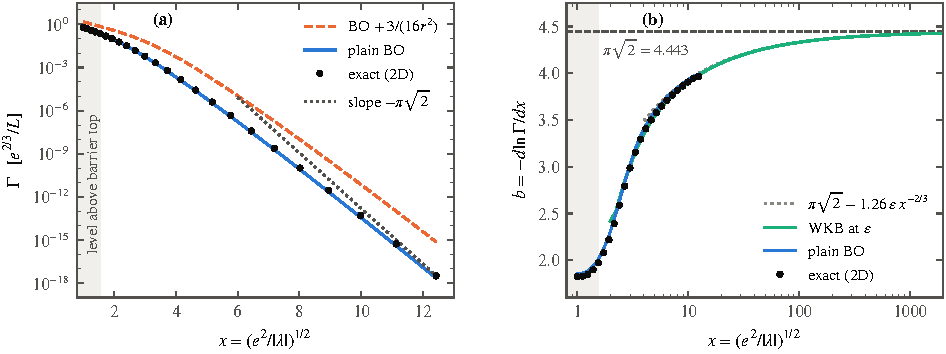
\includegraphics[width=\textwidth]{rep_v11_abelian_width}
\caption{Resonance of the abelian Higgs zero-mode problem against $x=(e^2/|\lambda|)^{1/2}$ (units $e=1$).
(a)~Width $\Gamma$ of the exact two-dimensional problem (points), of the plain Born--Oppenheimer model~(\ref{eq:v11-ab-UBO}) (solid) and of the model with the diagonal term $3/(16r^2)$ (dashed); dotted: slope $-\pi\sqrt2$ of the deep-well law through the last point.
(b)~Local exponent $b=-d\ln\Gamma/dx$: exact (points), plain Born--Oppenheimer (blue), and the WKB action of the Langer-corrected Born--Oppenheimer barrier at the computed energy (green), continued beyond $x=12.4$ with the extrapolated energy $\varepsilon_0=1.9026$; dotted: the leading-order form~(\ref{eq:v11-ab-Seps}); dashed: the deep-well value $\pi\sqrt2$. %
Shaded: the level lies above the barrier top.} %
\label{fig:v11-ab-width}
\end{figure}

\paragraph{Thresholds.}
A box that exists for $N$ light-crossing times keeps the resonance with probability $e^{-\Gamma N}$, and the threshold $\Lambda_c(N)$ solves $\Gamma N=\ln2$; we interpolate $\ln\Gamma$ by a cubic spline in $x$ and include a tenth of the difference from linear interpolation in the uncertainty.
Table~\ref{tab:v11-ab-thresholds} and Fig.~\ref{fig:v11-ab-threshold} give the results for $e=1$: $\Lambda_c=-0.2295$, $-0.09138$, $-0.05252$ and $-0.03123$ for $N=10$, $300$, $10^4$ and $10^6$, with uncertainties of at most $4\times10^{-5}$. %
For general $e$ the condition reads $e^{2/3}F(\Lambda_c)N=\ln2$, and $\lambda_c=e^2\Lambda_c$.

With a constant prefactor, $\Gamma=A\exp(-\pi\sqrt2\,x)$ gives $1/|\Lambda_c|^{1/2}=[\ln N+\ln(A/\ln2)]/(\pi\sqrt2)$, linear in $\ln N$ with slope $1/(\pi\sqrt2)$, so that $|\Lambda_c|^{1/2}\ln N\to\pi\sqrt2$ with corrections of order $1/\ln N$.
With Eq.~(\ref{eq:v11-ab-Seps}), $\ln(N/\ln2)=S(\varepsilon,x_c)+\ln T+O(1)$ gives $|\Lambda_c|^{1/2}\ln N=\pi\sqrt2\,[1-O((\ln N)^{-2/3})]$: the energy of the level adds a slower correction, which dominates as $N\to\infty$.
The computed thresholds approach the limit slowly: $|\Lambda_c|^{1/2}\ln N$ rises from $1.10$ at $N=10$ to $3.16$ at $N=10^{16}$, with local slope $d|\Lambda_c|^{1/2}/d(1/\ln N)$ from $0.52$ to $2.52$, and a straight line through $N=10^4$--$10^{16}$ has slope $1.76$ and intercept $+0.044$ (largest residual $0.006$). %
A constant prefactor as large as the effective prefactors of Table~\ref{tab:v11-ab-widths} would also give a slow approach, so these numbers describe the thresholds without separating the two corrections; the evidence for the energy term is the local exponent $b$ and its agreement with $dS(\varepsilon)/dx$. %
The continuation with the WKB action at the computed energy, anchored to the exact width at $x=12.4$, gives $|\Lambda_c|^{1/2}\ln N=3.75$, $3.98$ and $4.21$ at $N=10^{50}$, $10^{100}$ and $10^{300}$. %
This limit is a property of the abelian model, in which $\Gamma$ vanishes at $\Lambda=0$ because the potential $\frac32er$ then confines; for the Standard Model zero-mode model, which contains $\Delta V$, only the logarithmic dependence on the duration over the computed range is claimed (Sec.~\ref{sec:v11-static-box}).

At the Standard Model slope $\sigma_0=1.31$ ($e=0.8733$) the thresholds are $\lambda_c=-0.182$, $-0.071$, $-0.041$ and $-0.024$ for $N=10$, $300$, $10^4$ and $10^6$. %
The value at $N=300$, $\abelLamcSM$, is six times deeper than the static-box threshold $\lamc(300)=\lcAthree$ of the Standard Model (Sec.~\ref{sec:v11-static-box}). %
The abelian model lacks the two ingredients that make the Standard Model barrier more transparent: the one-loop energy $\Delta V$ of the non-zero modes, which roughly halves the barrier above the level (Sec.~\ref{sec:rb-size}), and the SU(2) zero-mode energy, through which the zero-point energy of the reduced Standard Model model rises with slope $\zpSlopeLo$--$\zpSlopeHi$ at $r=1$--$5$ instead of $\sigma_0$ (Sec.~\ref{sec:v11-static-box}). %
At $\lambda=-0.010$ the barrier of Eq.~(\ref{eq:v11-ab-UBO}) rises $3.25/L$ above the level at this slope, against $1.57/L$ in the reduced Standard Model model without $\Delta V$ and $0.72/L$ with it (Sec.~\ref{sec:rb-size}). %
Accordingly the abelian width there is $\Gamma=6.01\times10^{-12}/L$, against $\Gamma_{\rm 2D}=4.15\times10^{-4}/L$ in the reduced Standard Model model at fixed couplings (Table~\ref{tab:rb-widths}); its exponent $-\ln(\Gamma L\,e^{-2/3})=25.75$ lies well below the deep-well value $38.80$. %

\begin{table}[t]
\centering
\caption{Thresholds $\Gamma N=\ln2$ of the abelian Higgs model in units $e=1$, $\Lambda_c=\lambda_c/e^2$: exact two-dimensional widths (uncertainty at most $4\times10^{-5}$ in $\Lambda_c$), plain Born--Oppenheimer (BO) and BO with the diagonal term (BOD), the combination $|\Lambda_c|^{1/2}\ln N$ with its local slope against $1/\ln N$, and $\lambda_c$ at the Standard Model slope $\sigma_0=1.31$ ($e=0.8733$). In the deep-well limit $|\Lambda_c|^{1/2}\ln N\to\pi\sqrt2=4.443$.} %
\label{tab:v11-ab-thresholds}
\small
\begin{tabular}{@{}ccccccc@{}}
\toprule
$N$ & $\Lambda_c$ & $\Lambda_c^{\rm BO}$ & $\Lambda_c^{\rm BOD}$ & $|\Lambda_c|^{1/2}\ln N$ & $d|\Lambda_c|^{1/2}/d(1/\ln N)$ & $\lambda_c$ ($e=0.8733$) \\ %
\midrule
$10$ & $-0.22952$ & $-0.2315$ & $-0.1139$ & $1.103$ & $0.52$ & $-0.1818$ \\ %
$300$ & $-0.09138$ & $-0.0927$ & $-0.0539$ & $1.724$ & $0.94$ & $-0.0709$ \\ %
$10^{4}$ & $-0.05252$ & $-0.0533$ & $-0.0338$ & $2.111$ & $1.29$ & $-0.0405$ \\ %
$10^{6}$ & $-0.03123$ & $-0.0317$ & $-0.0216$ & $2.441$ & $1.64$ & $-0.0240$ \\ %
$10^{8}$ & $-0.02098$ & $-0.0213$ & $-0.0152$ & $2.668$ & $1.90$ & --- \\ %
$10^{10}$ & $-0.01517$ & $-0.0154$ & $-0.0114$ & $2.836$ & $2.10$ & --- \\ %
$10^{12}$ & $-0.01152$ & $-0.0117$ & $-0.0089$ & $2.966$ & $2.27$ & --- \\ %
$10^{14}$ & $-0.00908$ & $-0.0092$ & $-0.0071$ & $3.072$ & $2.40$ & --- \\ %
$10^{16}$ & $-0.00735$ & $-0.0075$ & --- & $3.159$ & $2.52$ & --- \\ %
\bottomrule
\end{tabular}
\end{table}

\begin{figure}[t]
\centering
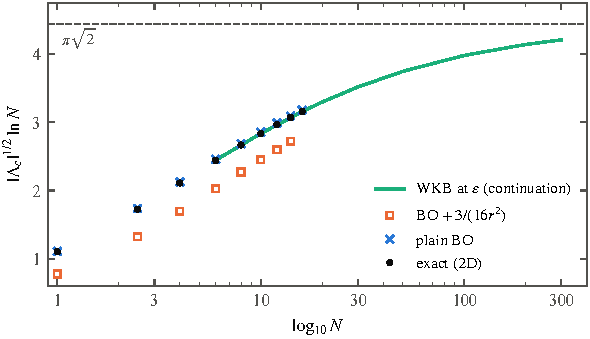
\includegraphics[width=0.62\textwidth]{rep_v11_abelian_threshold}
\caption{Thresholds $\Gamma N=\ln2$ of the abelian Higgs model: $|\Lambda_c|^{1/2}\ln N$ against $\log_{10}N$ for the exact two-dimensional widths (points), the plain Born--Oppenheimer model (crosses) and the model with the diagonal term $3/(16r^2)$ (squares), and the continuation with the WKB action of the Langer-corrected Born--Oppenheimer barrier at the computed energy, anchored to the exact width at $x=12.4$ (line). The deep-well limit $\pi\sqrt2$ (dashed) is approached only as $(\ln N)^{-2/3}$.} %
\label{fig:v11-ab-threshold}
\end{figure}

\paragraph{Accuracy of the Born--Oppenheimer approximation.}
The diagonal BO term follows from $\chi_0$.
With $\partial_\omega\chi_0=\bigl(\frac{3}{4\omega}-\frac{w^2}{2}\bigr)\chi_0$ and $\langle w^2/2\rangle=3/(4\omega)$,
\begin{equation}
\langle\partial_\omega\chi_0|\partial_\omega\chi_0\rangle={\rm Var}\Bigl(\frac{w^2}{2}\Bigr)=\frac14\sum_{i=1}^3{\rm Var}\bigl(w_i^2\bigr)=\frac14\cdot3\cdot2\Bigl(\frac{1}{2\omega}\Bigr)^2=\frac{3}{8\omega^2},
\label{eq:v11-ab-var}
\end{equation}
and with $\partial_r=e\,\partial_\omega$
\begin{equation}
\tfrac12\,\langle\partial_r\chi_0|\partial_r\chi_0\rangle=\frac12\,e^2\,\frac{3}{8e^2r^2}=\frac{3}{16r^2},
\label{eq:v11-ab-diag}
\end{equation}
independent of $e$.
This is the Born--Huang term of the $\bm w$ motion, $B_w$ of Eq.~(\ref{eq:rb-BH}), which in the Standard Model takes this form at small $r$ [Eq.~(\ref{eq:rb-Bw})] and in the abelian model has it at every $r$.
The function $\partial_\omega\chi_0$ is proportional to the first radial excitation $\chi_1$ of the s-wave oscillator, so that the diagonal term is $\frac12A^2$, where $A=\langle\chi_1|\partial_r\chi_0\rangle=(3/8)^{1/2}/r$ is the only non-adiabatic coupling of the ground channel, to a channel $2er$ higher.
Adding Eq.~(\ref{eq:v11-ab-diag}) to Eq.~(\ref{eq:v11-ab-UBO}) gives $U_{\rm BOD}=\frac32er+1/(16r^2)+\lambda r^4/4$, with the Frobenius exponent $a=1.1124$ in place of $1/2$. %
For a bound ground state the BO energy without the diagonal term is a lower bound and with it an upper bound; the computed resonance energies obey $\varepsilon_{\rm BO}<\varepsilon<\varepsilon_{\rm BOD}$ at every $\Lambda$. %

The plain BO model places the level $0.096$--$0.103$ below the exact one and gives widths within $\abelBOdev$: $\Gamma_{\rm BO}/\Gamma$ falls from $1.02$ at $\Lambda=-1$ through $0.85$ at $\Lambda=-0.030$ to $0.72$ at $\Lambda=-0.0065$, and $b_{\rm BO}-b=+0.02$ to $+0.04$ (Table~\ref{tab:v11-ab-widths}, Fig.~\ref{fig:v11-ab-width}). %
The slow drift of $\Gamma_{\rm BO}/\Gamma$ follows from the energy error through Eq.~(\ref{eq:v11-ab-Seps}), $\Delta S\approx3.78\times0.10\,x^{1/3}$, and the BO thresholds lie within $1.5\%$ of the exact ones (Table~\ref{tab:v11-ab-thresholds}). %
With the diagonal term the level lies $0.50$--$0.65$ too high, the widths are too large by factors of $2.5$ ($\Lambda=-1$) to $233$ ($\Lambda=-0.0065$), $b$ is too low by $0.2$--$0.9$, and the thresholds are $22$--$50\%$ shallower. %
The exact level lies at $13$--$17\%$ of the bracket $[\varepsilon_{\rm BO},\varepsilon_{\rm BOD}]$, so that the non-adiabatic couplings, leading at second order, cancel $83$--$87\%$ of the shift produced by the diagonal term. %
The reason is the absence of a small parameter.
By the scaling~(\ref{eq:v11-ab-scaling}) the $w$ frequency in the well, $er$ at $r\approx e^{-1/3}$, and the energy scale of the $r$ motion are both proportional to $e^{2/3}$, so their ratio does not depend on the coupling; in the well the kinetic energy of the $r$ motion, about $\varepsilon/3$ by the virial theorem for a linear well, is comparable with the gap $2er$, and the second-order energy of the coupling $A$, of order $A^2\langle p_r^2\rangle/(2er)$, is of the same order as $\frac12A^2$.
Only under the barrier, at $r\approx|\Lambda|^{-1/3}$ in units $e=1$, is the $w$ motion fast.
A one-dimensional reduction with the diagonal BO term is therefore unsuitable for quantitative widths, and the plain BO model, or better the BO barrier at the exact energy, is accurate to tens of per cent.

The reduced Standard Model model of Sec.~\ref{rep:h-reduced} solves $r$ and $|\bm w|$ together and does not use the diagonal term for $\bm w$.
Its hypercharge mode also has a frequency that vanishes linearly as $r\to0$, and Sec.~\ref{rep:h-reduced} found the same pattern there: the two-dimensional energy lies at $15.5\%$ of its BO bracket at $\lambda=0$, and nearly all of $B_w$ is spurious (Table~\ref{tab:rb-lam0} and the discussion of the mechanism). %
The abelian model, solved without any reduction, shows that this is a property of a fast mode whose frequency vanishes linearly in the slow coordinate, independent of the approximations of Sec.~\ref{rep:h-reduced}, and that a one-dimensional reduction with that term would overestimate the widths by orders of magnitude.
The SU(2) modes, which the magnetic quartic term keeps stiff at small $r$, enter the reduced model through the conditional Gaussian with the Born--Huang term $B_x\le0.012$ for $r\le3$ (Table~\ref{tab:rb-BH}); the full-dimensional calculation of Secs.~\ref{sec:v18-problem}--\ref{sec:v18-mc} tests that part directly. %

\paragraph{Compactness of the holonomy.}
The truncation treats $\bm w$ as non-compact.
A large gauge transformation shifts each $ew_i$ by $2\pi$, so the configuration space of the constant connections is the fundamental domain $|ew_i|\le\pi$, and near its boundary a charged mode of non-zero momentum becomes as light as the constant mode, where the zero-mode Hamiltonian no longer applies.
In the converged resonance wave functions, inside the radius of the barrier top, the probability that $e|\bm w|$ exceeds $\pi$, an upper bound on the probability that some component leaves the domain, is $1.8$--$2.6\times10^{-3}$ for $e=1$, $5.5$--$8.1\times10^{-4}$ for $e=0.873$ ($8.0\times10^{-4}$ at $\lambda=-0.010$) and $3.2$--$5.9\times10^{-7}$ for $e=0.5$. %
Beyond $e|\bm w|=\pi/2$ it is $23$--$26\%$, $16$--$19\%$ and $1.9$--$2.4\%$; the ranges cover $\Lambda=-1$ to $-0.0065$, with the narrow resonances at the upper ends, and direct calculations at $e=0.873$ reproduce the values obtained by scaling. %
The non-compact treatment therefore affects a probability below $\abelHolonomy$ at the Standard Model slope. %
Its effect on $\Gamma$, through the energy of the level, was not computed; by Eq.~(\ref{eq:v11-ab-Seps}), $\delta\ln\Gamma\approx3.78\,x^{1/3}\,\delta\varepsilon\approx8\,\delta\varepsilon$ at $e=0.873$ and $\lambda=-0.010$, so a level shift of order $10^{-3}$ would change $\Gamma$ at the per-cent level. %
The wave function is, however, not deep inside the domain for $e\approx0.87$--$1$: about a fifth of the probability lies beyond half of it. %

\paragraph{Without the gauge modes.}
For $e\to0$ at fixed $\lambda<0$ the problem is $-\frac12\nabla_\phi^2+\frac\lambda4|\bm\phi|^4$ on the plane, whose potential decreases monotonically from zero: there is no well, no barrier and no quasi-bound state.
Scaling $r\to\mu r$ with $\mu^6=-1/|\lambda|$ maps the inverted quartic to $|\lambda|^{1/3}e^{-i\pi/3}$ times the quartic oscillator $-\frac12\nabla^2+\frac14r^4$, so that every complex-scaled eigenvalue lies on the ray $\arg E=-60^\circ$, with $\Gamma/{\rm Re}\,E=2\sqrt3$ for every $\lambda$.
At $\lambda=-0.03$ the lowest one is $E=0.14457-0.25040\,i$, at $\arg E=-60.000000^\circ$. %
This pole is fixed by the scaling of the inverted quartic and is not a narrow resonance.
In the form~(\ref{eq:v11-ab-Hu}) the reduced potential $-1/(8r^2)+\lambda r^4/4$ is not monotonic: it has a maximum of negative height $-\frac{3}{16}(4|\lambda|)^{1/3}$ at $r=(4|\lambda|)^{-1/6}$.
This maximum is not a barrier, since $-1/(8r^2)$ is the $m=0$ kinetic term of the plane, which the Langer substitution removes; the potential of the problem, $\lambda|\bm\phi|^4/4$, is monotonic.
The narrow resonance of the model is therefore due to the gauge zero modes, as for the gauge zero-mode switch of the Standard Model calculation (Sec.~\ref{sec:v11-kappa}).

\paragraph{What the test establishes.}
\emph{Proved.} The zero-mode problem of the abelian Higgs model reduces exactly to $(r,s)$; its resonance obeys Eq.~(\ref{eq:v11-ab-scaling}); the diagonal BO term is $3/(16r^2)$. %

\emph{Under stated conditions}, in the WKB approximation for the Langer-corrected BO barrier, which is asymptotically exact as $x\to\infty$: the deep-well exponent is $\pi\sqrt2\,x$, and the energy of the level lowers the barrier action by $3.78\,\varepsilon\,x^{1/3}$ at leading order. %

\emph{Found numerically}, with relative precision of order $10^{-8}$ internally and $10^{-6}$ against the independent method at $-0.416\le\Lambda\le-0.0155$ (the blind recalculation of Sec.~\ref{sec:v11-blind-abelian} also covers $\Lambda=-1$ and $-0.01003$): the gauge zero modes alone confine the negative quartic, with widths from $0.61$ to $3.2\times10^{-18}$; the local exponent rises from $1.8$ to $4.0$ and is reproduced by the WKB action of the BO barrier at the computed energy; the plain BO widths lie within $30\%$ of the exact ones, and the widths with the diagonal term are too large by up to $233$; the weight beyond the fundamental domain of the holonomy is below $10^{-3}$ for $e\le0.87$. %

\emph{Expected}, from the WKB continuation: $b=4.28$ and $4.42$ at $x=60$ and $1000$, and the approach of $|\Lambda_c|^{1/2}\ln N$ to $\pi\sqrt2$; these rest on the barrier action at an extrapolated energy, with a prefactor ratio that varies slowly ($0.80$ to $0.757$ over $x=3$--$12.4$). %

\emph{Outside the test.} The model contains no $\Delta V$, no SU(2) modes, no fermions and no cross terms; it tests the mechanism and the WKB form of the width at the resonance energy, whereas the deep-well law with a constant prefactor holds only asymptotically, and it does not test the numbers of the Standard Model, whose threshold at $N=300$ is six times shallower than that of the model at the same zero-point slope. %
It does not test the conditional Gaussian of the SU(2) modes or the DMC shape correction, which the full-dimensional calculation of this section tests, and it omits the compactness of the holonomy and the light charged modes near the boundary of the fundamental domain, whose weight it bounds.


\section{Independent reimplementations}\label{rep:v-blind}

Every ingredient of the Higgs criterion, the shape theorem and its survival levels, the readability of the fossil and the key literature judgments were recomputed by separate calculations that did not use our main code.
This section records what each check was given, what it reproduced, to what precision, and which corrections it caused.
We find that the blind reimplementation of the reduced Higgs chain reproduces its critical top masses to $0.005\GeV$, against a pass criterion of $0.05\GeV$ fixed in advance; that the blind cross-term calculation confirms that the cross terms destabilize the zero mode, with a shift within $0.010\GeV$ of the main calculation; that the blind Standard Model mapping reproduces $\lambda(\mub)$ to $4\times10^{-6}$ with the same matching and explains a scheme difference of $0.043\GeV$; and that the blind shape calculation reproduces the real-moment theorem, the floor and the survival levels within their statistical errors. %
No check failed its pass criterion.
Most of them led to corrections, all of which are included in Part~I and recorded in Part~III; Table~\ref{tab:v19-summary} at the end of the section summarizes them.

\subsection{Protocol and levels of independence}\label{sec:v19-protocol}

The reimplementations (see the Acknowledgments) were made at three levels of independence; each check is labeled by the identifier of its record.
\begin{description}
\item[Blind (third stage: keystone, V1--V6).] Each check received a written specification with the model definitions, the inputs and the pass criteria, an earlier draft of the paper as an external anchor (for example its full-dimensional DMC value at $\lambda=0$), and access to the literature.
It had no access to the derivations, code and results of the main calculation or to the records of the other checks.
It recorded its results, with a time stamp and the SHA-256 hash of its code, before it received any number of the main calculation; the comparison was compiled afterwards.
\item[Compute first (first and second stages: R14, R15).] Each check computed its own numbers before opening the results of the main calculation, and compared afterwards.
Some of these checks reused earlier independent code that the main calculation also uses (R15 checks of the matching and of the real-time evolution), and in one case the result tables of the main calculation were seen before the computation (R15 check of the two-dimensional model), which makes that check only partly independent; we state these limitations below.
\item[Semi-blind (T19).] The check used only the claims and the non-numerical parts of the derivations, saved its own results, and then opened the result tables of the main calculation; one accidental exposure of a few of their rows is recorded in its report.
\end{description}
A read-only consistency audit (Sec.~\ref{sec:v19-audit}) compared about 420 quoted values with their source files.

\subsection{Keystone: the reduced Higgs chain}\label{sec:v19-keystone}

The keystone check reimplemented the full Higgs chain of the second stage: the consistent one-loop finite-volume matching (Sec.~\ref{rep:h-matching}), the two-dimensional $(r,s)$ model (Sec.~\ref{rep:h-reduced}) and the hazard along the turn (Sec.~\ref{rep:h-survival}), with $hL_b=0.00437243$, the earlier Standard Model mapping and without cross terms. %
The specification defined the model in six parts and allowed only the earlier draft and the literature.
The reimplementation uses its own proper-time finite-volume one-loop functions, including a closed form of the Coulomb-mode contribution that agrees with Wolfram Language to 25 digits; at small $r$ its $V_1/(r^2/2)=-0.10704543$ equals the zero-mode mass formula of the draft. %
Its renormalization-group code agrees with Wolfram \texttt{NDSolve} to $3\times10^{-15}$; it computed resonances both as Siegert states and with complex absorbing potentials, in one dimension and in the multichannel two-dimensional model, and it computed its own DMC correction $\delta E(r)$ of the SU(2) shape, validated on pure SU(2), where it gives $2.6860\pm0.0025$ against L\"uscher's $2.68523$~\cite{Luscher:1982ma}. %
Table~\ref{tab:v19-keystone} compares the results.

\begin{table}[t]
\centering
\caption{Keystone check of the reduced Higgs chain (model of the second stage: earlier Standard Model mapping, no cross terms; $\alpha_s=0.1180$). ``Blind'' values were fixed before the comparison.}
\label{tab:v19-keystone}
\small
\begin{tabular}{@{}lcc@{}}
\toprule
Quantity & Blind & Main \\
\midrule
$\lambda(\mub)$ & $-0.0101929$ & $-0.010193$ \\ %
$y_t(\mub)$ & $0.428359$ & $0.42836$ \\ %
$L\varepsilon_0(\lambda=0)$, 2D$_{\rm G}$ & $4.50769$ & $4.507701$ \\ %
$L\varepsilon_0(\lambda=0)$, 1D & $4.59855$ & $4.598545$ \\ %
$L\varepsilon_0(\lambda=0)$, with DMC shape & $4.45078$ & $4.45086$ \\ %
$L\Gamma(\lambda=-0.010)$, 2D$_{\rm G}$ & $5.3183\times10^{-4}$ & $5.318\times10^{-4}$ \\ %
$L\Gamma(\lambda=-0.010)$, 1D & $9.8711\times10^{-4}$ & $9.8711\times10^{-4}$ \\ %
static $\lambda_c$ ($P=0.9/\allowbreak 0.5$), 2D$_{\rm G}$ & $-0.009424/\allowbreak{-}0.012613$ & equal to $<10^{-6}$ \\ %
$\Pone(172.2/\allowbreak 172.6/\allowbreak 173.0)$ & $0.9792/\allowbreak 0.8210/\allowbreak 0.4371$ & $0.97920/\allowbreak 0.82098/\allowbreak 0.43738$ \\ %
$m_c$, one-dimensional model (GeV) & $172.349/\allowbreak 172.768/\allowbreak 173.187$ & $172.349/\allowbreak 172.768/\allowbreak 173.187$ \\ %
$m_c$, 2D$_{\rm G}$ (GeV) & $172.467/\allowbreak 172.941/\allowbreak 173.420$ & $172.467/\allowbreak 172.941$/--- \\ %
$m_c$, 2D with own DMC shape (GeV) & $172.521/\allowbreak 173.017/\allowbreak 173.520$ & $172.518/\allowbreak 173.014/\allowbreak 173.515$ \\ %
$dm_c/d\alpha_s$ (GeV) & $\approx388$ & $\approx387$ \\ %
\bottomrule
\end{tabular}
\end{table}

The critical masses agree to $0.005\GeV$ at all three levels, against the pass criterion of $0.05\GeV$, and all intermediate quantities agree to $10^{-4}$ or better; the blind numerical error on $m_c$ is estimated at $0.005\GeV$ or less. %
The blind DMC shape correction has a statistical sensitivity of about $\pm0.02\GeV$ in $m_c$, within which it agrees with the correction of the main calculation.
One methodological error of the blind code, the principal square root on closed channels in the outgoing condition, produced spurious roots and was fixed before the comparison.
The check does not cover the cross terms or the NNLO mapping, which V2 and V1 check, and it lists as open the non-Gaussian effects beyond $\delta E(r)$, two-loop matching, holonomy fluctuations, the top quark at $m_tL\approx1$--$1.5$ and the hazard prescription itself (Secs.~\ref{rep:h-budget} and~\ref{rep:v-fulldim} treat them). %

\subsection{V2: the cross terms}\label{sec:v19-v2}

The second blind check computed the cross terms between the zero mode and the non-zero modes from the model definitions, with the curvatures of the earlier internal draft as the only anchor.
It used a twist approximation in which each charged component receives a momentum shift, with periodic bosons excluding $n=0$ and antiperiodic fermions; its direction-averaged twisted sums agree with the $\theta=0$ limit and with Bessel--Poisson sums to $10^{-16}$. %
At $r=0$ it reproduced the holonomy curvatures $-0.39261$, $-0.24209$ and $+0.70036$ (SU(3), SU(2), hypercharge; Sec.~\ref{rep:h-cross}). %
It found that the soft hypercharge direction, unstable for $r\lesssim0.78$ when only Higgs fluctuations are kept, is stable everywhere when all fields are included ($\frac12\kappa_{\rm mean}=+0.068$). %
Its width ratios at $\lambda=-0.008$, $-0.010$ and $-0.0143$ are $1.217/\allowbreak 1.177/\allowbreak 1.122$ (SU(3)--top), $0.646/\allowbreak 0.683/\allowbreak 0.748$ (SU(2)), $2.039/\allowbreak 1.914/\allowbreak 1.702$ (hypercharge) and $1.613/\allowbreak 1.552/\allowbreak 1.444$ in total, against $1.21/\allowbreak 1.17/\allowbreak 1.12$, $0.65/\allowbreak 0.69/\allowbreak 0.75$, $2.06/\allowbreak 1.93/\allowbreak 1.72$ and $1.63/\allowbreak 1.57/\allowbreak 1.46$ in the main calculation. %
The total shift of the critical mass is
\begin{equation}
\Delta m_c^{\rm blind}=-0.081,\ -0.117,\ -0.157\GeV,\qquad \Delta m_c^{\rm prod}=-0.085,\ -0.124,\ -0.167\GeV
\label{eq:v19-v2}
\end{equation}
at $\Pone=0.9$, $0.5$ and $0.1$, a difference of $0.004$--$0.010\GeV$ within both error estimates (numerical $\lesssim0.005\GeV$ and model $\pm0.015\GeV$ in the blind report). %
The difference is kept as an item of the error budget (Sec.~\ref{rep:h-budget}).
The check confirmed blindly that the cross terms destabilize the zero mode, which retracted the stabilizing interval of the second stage, and it identified the instability of the soft direction as an artifact of keeping only Higgs fluctuations (Part~III).
It was compared with the third-stage calculation that preceded the one-loop vev-mixing, Coulomb and top-chiral terms; those terms, which largely cancel and move the final critical masses by $+0.005$ to $+0.007\GeV$, were checked only within the main code (Sec.~\ref{rep:h-cross}). %

\subsection{V1: the Standard Model mapping}\label{sec:v19-v1}

The third blind check mapped $(m_t,\alpha_s,M_h)$ to the $\MSbar$ couplings at $\mub$ with at least one matching implementation different from SMDR, as the specification required.
It used \texttt{mr} (Kniehl--Pikelner--Veretin), compiled with MinGW g++~5.3, and SMDR~1.3 as a second implementation~\cite{Martin:2019lqd}, its own $\alpha_s$ running and its own renormalization-group equations; all 276 three-loop monomials of the $\beta$ functions match the published ones. %
At $(m_t,\alpha_s,M_h)=(172.60,0.1180,125.13)$ it gives with \texttt{mr}
\begin{equation}
\lambda(\mub)=-0.010055,\quad y_t=0.427896,\quad g_2=0.527828,\quad g_Y=0.442586,\quad g_3=0.535646,
\label{eq:v19-v1}
\end{equation}
with $d\lambda(\mub)/dm_t=-0.006592\GeV^{-1}$ and $\mtbar(\mtbar)=162.820\GeV$. %
Its benchmarks against Buttazzo et al.\ pass for $\lambda(m_t)$ and $y_t$ and fail for $g_3$ by an unexplained $0.0018$; its critical mass in the convention of Bednyakov et al.\ is $171.432\GeV$ against $171.44\GeV$. %
After unblinding, the \texttt{mr} value of $\lambda(\mub)$ differs from the main value, $-0.009774$, by $-2.8\times10^{-4}$, or $0.043\GeV$ in $m_t$; this is a difference between two organizations of the two-loop matching. %
With SMDR matching and its own running the blind value is $-0.009778$, within $4\times10^{-6}$ of the main value. %
The check led to three corrections.
\begin{enumerate}
\item \texttt{mr} must run single-threaded, because its OpenMP build has a race condition in TSIL.
\item The matching-scale error differs by a factor of about ten between the two implementations: SMDR with all scales halved or doubled gives $+0.033/\allowbreak{-}0.019\GeV$, which V1 reproduced bit for bit, while \texttt{mr} gives $+0.173/\allowbreak{-}0.358\GeV$, as in Bednyakov et al.; the cause is the non-QCD logarithms of the $G_F$ scheme combined with a cancellation between the $m_t$ and $M_h$ terms in SMDR. %
\item The recommended Standard Model error, $\pm0.07\GeV$ for $\mtbar$ and $\pm0.10\GeV$ for the pole mass, replaced the earlier $\pm0.047$ and $\pm0.086\GeV$ and is used in the papers (Sec.~\ref{rep:h-smmap}). %
\end{enumerate}

\subsection{V3: the claims layer and the robustness of the inputs}\label{sec:v19-v3}

The fourth blind check recomputed the marginalization, the Bayes factors, the exclusion thresholds and the experimental reach from the table of $\Pone(m_t,\alpha_s)$ of the third stage and the model-error budget supplied in the specification, and the sensitivities to the duration of the turn, to $\fzm$ and to the preparation weight.
Two independent integrators (a grid and a Monte Carlo with $2\times10^6$ samples) agree to $3.4\times10^{-4}$, and the experimental inputs were checked against the pages of the cited reports. %
For the direct mass it gives $\Pbar=0.725$ with the $68\%$ range $[0.380,0.989]$, against $0.727$ and $[0.384,0.989]$ in the main calculation; $|\ln B|\le0.71$; $\Pone=0.1$ at $173.062/\allowbreak 173.412/\allowbreak 173.761\GeV$ for $\alpha_s=0.1171/\allowbreak 0.1180/\allowbreak 0.1189$; a measured centre of $174.18\GeV$ for a $95\%$ exclusion; and a present separation of $172.6$ and $173.3\GeV$ at $1.5\sigma$. %
These are the numbers of the third-stage model; the final model shifts them as described in Sec.~\ref{rep:h-budget}.
Changing $hL_b$ by factors $0.9$ and $1.1$ moves $m_c$ by $-0.020/\allowbreak{-}0.032/\allowbreak{-}0.049$ and $+0.018/\allowbreak{+}0.030/\allowbreak{+}0.046\GeV$, and the blind preparation weight is $w_0=0.991$--$0.996$. %
The check passed with four corrections, all adopted.
\begin{enumerate}
\item The main code combined asymmetric errors in two different ways in different places; the equal-mass convention is now used throughout (Sec.~\ref{rep:h-budget}), which changes the variant of Bednyakov et al.\ to $0.67$ and its quoted range to $0.62$--$0.67$.
\item The separation reachable at the HL-LHC depends on the assumed precision of $\alpha_s$; it is now quoted as about $1.7\sigma$ to $2.5\sigma$.
\item The dependence on the duration of the turn has two correct but different measures, the secant over one e-fold and the local derivative; both are now named.
\item The flat prior on $[150,200]\GeV$ was in fact applied on a grid over $[160,186]\GeV$; corrected, $B_{\rm sel}=1.584$ instead of $1.459$ and its upper bound $2.18$ instead of $2.007$ (third-stage model). %
\end{enumerate}

\subsection{V4: the shape side}\label{sec:v19-v4}

The fifth blind check recomputed the real-moment theorem, the floor, the function $G(|t_x|)$, the nonlinear survival that defines $t_*$, the next-order floor, the emptiness budget and the preparation window (Secs.~\ref{rep:gate} and~\ref{rep:quantum-shape}).
It had the earlier draft and the method sections of two derivations without their tables, and an addendum to its specification required $N\ge2048$ samples for every quantity at the $99\%$ level.
It computed the linear transfer three ways (two ODE integrators and Wolfram Language, agreeing to $10^{-8}$), the floor in closed form and by ODE (to $10^{-12}$), and the Ewald eigenvalues $1902.2404$ and $-893.2029$; the nonlinear five-dimensional integration used common random numbers with $N=2048$ per point. %
It gives $\kappa_E=19.32654$, $\sigma_{\rm floor}=0.10406$, $G(|t_x|)=2.3955$, $45.1258$ and $314.090$ at $h|t_x|=0.1$, $0.5$ and $1$, and $G(\infty)=1349.24$, against $\sigma_{\rm floor}=0.1037$ and $G=2.395$, $45.10$ and $313.8$ in the main calculation; the differences of $0.3\%$ come from the input $X$ ($2269.2$ against $2282.5$). %
Its survival thresholds are $h|t_*|=0.360$ ($90\%$) and $0.243$ ($99\%$), against $0.355\pm0.003$ and $0.237$ in the main calculation repeated with $N=2048$; with only $N=256$ the blind code gives $0.373$ and $0.264$, which shows why the larger samples were needed. %
Its emptiness budget is $4.7616$, $4.8976$ and $5.0473$ quanta for the three values of $\fzm$, and its latest preparation $7.2640$ e-folds. %
The check passed; together with T19 it caused the rerun of all $99\%$-level points with $N\ge2048$, and the theorem is now stated with $|t_x|\lesssim0.35/h$ ($0.24/h$) (Sec.~\ref{rep:quantum-shape}).

\subsection{V5: universality and the bound during inflation}\label{sec:v19-v5}

The sixth blind check recomputed the bound on $\xiH$ from Higgs stability during the plateau and the scaling of $\lambda_c$ (Sec.~\ref{rep:h-universality}).
With its own three-loop running, a curved-space renormalization-group-improved potential and Hawking--Moss counting over the past light cone, it gives $\xi_{\rm EW,inf}=0.05032/\allowbreak 0.05637/\allowbreak 0.06151$ and $\xi_{\rm inf}(\mub)=0.03224/\allowbreak 0.03940/\allowbreak 0.04550$ at $m_t=172.2/\allowbreak 172.6/\allowbreak 173.0\GeV$, and $0.0487/\allowbreak 0.0547/\allowbreak 0.0599$ after subtracting its offset in the reproduction of Mantziris, Markkanen and Rajantie (2021), against $0.04877/\allowbreak 0.05512/\allowbreak 0.06044$ (electroweak) and $0.03030/\allowbreak 0.03781/\allowbreak 0.04413$ ($\mub$) in the main calculation. %
Its Hawking--Moss exponent agrees between Python and Wolfram Language to $7\times10^{-14}$ relative. %
For $\lambda_c$ it gives $d\lambda_c/d\ln\eta_\infty=+0.00220$ and coupling derivatives that differ from the final model by $10$--$20\%$, as expected between the static second-stage model it used and the final hazard. %
The check passed (differences $\le0.002$ in $\xi$).

\subsection{V6: key literature judgments}\label{sec:v19-v6}

The seventh blind check answered six questions about the literature from the original papers, with page and equation numbers, before it read the literature notes of the project.
It confirmed that the applicable bound for a minimally coupled plateau is that of Mantziris, Markkanen and Rajantie (2021), $\xi_{\rm EW}\ge0.059^{+0.007}_{-0.009}$, and that their 2022 bound $\xi_{\rm EW}\gtrsim0.1$ applies only to $R^2$ gravity; and that the topology searches require $L>0.97$ (Planck 2015) or $L>0.985$ (COMPACT) in units of the diameter of the last-scattering sphere, so that the window $1.02$--$1.04\,\dLSS$ is allowed. %
It found that the earlier notes stated the relation to Branchina et al.\ too strongly and missed three references (Arkani-Hamed, Dubovsky, Nicolis and Villadoro 2007; Hamada and Shiu 2017; Arnold, Fornal and Wise 2010); the papers now cite them and state the relation conditionally. %

\subsection{T19: items left unverified after the second stage}\label{sec:v19-t19}

The semi-blind check T19 recomputed the nonlinear amplitude thresholds of the shape, a layer of the divergences of the microwave-background calculation, the closed-form scaling of the fossil and three older items.
With $N=2048$ it gives the survival $1.000/\allowbreak 0.987/\allowbreak 0.818/\allowbreak 0.365/\allowbreak 0.067/\allowbreak 0.0015$ for amplitude factors $s=1/3/5/10/20/40$, against $1.000/\allowbreak 0.973/\allowbreak 0.824/\allowbreak 0.367/\allowbreak 0.062/\allowbreak 0.000$ in the main calculation with $N=256$, and $s_{50}/s_{90}/s_{99}=8.18/\allowbreak 4.28/\allowbreak 2.95$ against $8.2/\allowbreak 4.2/\allowbreak 2.2$. %
The main calculation, repeated with $N=2048$, then gave $s_{99}=2.76$ (range $2.66$--$2.96$); the two values are about $2\sigma$ apart, and the papers quote $s_{99}\approx2.8$--$2.95$. %
Its divergences for $\ell\le40$ and $\ell\le30$, $7.21855$ and $5.25558$, agree with the main calculation ($7.22572$, $5.26140$) to $0.1\%$, within the $1\%$ criterion, and it reproduces the scaling function $F(19.32)=24.550106$. %
It found that the plateau background adds $0.4$--$0.8$ percentage points of survival, that the Moyal correction changes a variance by a factor $0.99989$, and that the photon-pair branch has its centre at $4.956$ with a $5$--$95\%$ range $2.98$--$11.9$. %
Its corrections ($s_{99}\approx2.95$ and $\sigma(99\%)\approx0.31$ instead of $2.2$ and $0.24$; ``centre $\approx5$, $90\%$ interval $3$--$12$'' for the photon pair) were adopted (Part~III).

\subsection{Checks of the first and second stages}\label{sec:v19-early}

\paragraph{R14, Higgs survival (first stage).}
The first independent check of the Higgs survival computed its own running, Ewald and Epstein-zeta matching with the tachyonic branch, Numerov integration with a WKB outgoing condition, complex Muller roots and pole continuation along the turn.
It reproduced the width of the first-stage model at $\lambda=-0.010$, $2.05075\times10^{-3}$ against $2.051\times10^{-3}$, and the first-stage critical masses to $0.02\GeV$ ($172.20/\allowbreak 172.57$ against $172.22/\allowbreak 172.59\GeV$). %
Its main finding changed the physics: with minimal coupling $\xiH=0$ the term $a''/a$ in the zero-mode mass makes the width grow from $1.90\times10^{-3}$ at $\tau=3$ to $1.15$ at $\tau=5$, almost independently of $m_t$, so that survival requires a curvature coupling; this is the origin of the condition on $\xiH$ (Sec.~\ref{rep:h-universality}) and of the choice $\xiH=1/6$ in all later hazards. %
It also noted that the first-stage errors omitted the reduction (estimated then at $\pm0.1$--$0.15\GeV$) and a gauge dependence of about $0.25\GeV$; both were removed by the consistent matching and the two-dimensional model.
It found that the calibration of Buttazzo et al.\ refers to the non-reduced Planck mass.

\paragraph{R14, state selection (first stage).}
The check of the inheritance of the shape state used the exact hypergeometric transfer matrix at $40$--$90$ digits and two ODE integrations agreeing to nine digits, and reproduced $G(|t_x|)$ to eight digits ($G=2.395171$, $45.09679$ and $313.7866$ at $h|t_x|=0.1$, $0.5$ and $1$; $G(\infty)=1347.651$). %
It corrected six statements of the first draft of the theorem, among them the factor by which a state real in the freezing region exceeds the floor ($19.6$ instead of $36.7$ at the freeze edge) and the claim that the future branch cannot fall below the floor; the corrected theorem is that of Sec.~\ref{rep:quantum-shape}. %

\paragraph{R15, matching (second stage).}
With a new basis-free decomposition of the Coulomb-mode energy and Wolfram cross-checks to $3.8\times10^{-9}$, the check reproduced the matched width $9.871149\times10^{-4}$ exactly, the static thresholds to $10^{-6}$ and the critical masses $172.3485/\allowbreak 172.7681\GeV$ against $172.3486/\allowbreak 172.7680\GeV$. %
It shares the hazard code with the main calculation.
It found that the non-adiabatic effect is about $\pm0.004\GeV$ rather than $\le0.002\GeV$ when the top quark is treated with Dirac-pair matrix elements.

\paragraph{R15, real-time evolution (second stage).}
An independent time-dependent Schr\"odinger solver in the radial frame with a moving absorber reproduced $w_0=1.0019$, the asymptotic hazard survival $0.47706$ against $0.4770$, and $\xi_c(172.6)=0.0723\pm0.0025$ against $0.072\pm0.003$ on the potential of that stage. %
It corrected three statements: the running prescription $\lambda(1/L)$ is frozen after $\tau=7$ in the code; a Gaussian truncated at the origin gives $w_0=0.743/\allowbreak 0.857$ and is not in the domain of the Hamiltonian, which led to the rule for $w_0$ of Sec.~\ref{rep:h-survival}; and the insensitivity to the switching time holds only for one of the two prescriptions.

\paragraph{R15, two-dimensional model (second stage).}
A B-spline Galerkin method in $r$ with a DVR in $s$ and absorbing-potential trajectories reproduced the $\lambda=0$ energies to $10^{-6}$, the width ratios $\Gamma_{\rm 2D}/\Gamma_{\rm 1D}=0.39136/\allowbreak 0.42078/\allowbreak 0.48362$ against $0.391/\allowbreak 0.421/\allowbreak 0.484$, and the critical masses $172.509/\allowbreak 173.002\GeV$ of the linearized conversion. %
Because the result tables were seen before the computation, the check is only partly independent.
Its estimate of the cross terms ($+0.05/\allowbreak{+}0.07\GeV$, stabilizing) was based on Higgs-only curvatures and was reversed by the third stage (Sec.~\ref{sec:v19-v2}).

\paragraph{R15, time symmetry (second stage).}
The check of the origin of time-reflection symmetry derived the energy variance of the centred Gaussian family symbolically, found that among general real states the infimum of the variance is zero, and corrected five statements: ``single classical history'' is an extra assumption (with an explicit counterexample), the width of the Airy region, the closed contour required by Hartle--Hawking, the restriction of minimal variance to the Gaussian family, and the statement that the homogeneous cap is impossible. %
It also found that a header comment of the nonlinear survival code stated a pinch threshold of $10^{-6}$ while the code uses $10^{-3}$.

\paragraph{R15, the separate line of calculation.}
The checks of Sec.~\ref{rep:v-conditional} recomputed the curved-cigar shape Hessians in closed form (main-code finite differences within $6.4\times10^{-6}$; coefficient $\frac{73}{3}\,\mathrm G=22.288496124979$), the width $\sigma_\phi=0.0097372$ of the joint state and its lower bound $0.935075$ (linear) and $0.935278$ (nonlinear), and the ensemble layer of the readability: peak $0.350$ at $1.076\,\dLSS$ against $0.344$ at $1.075$, window $[1.016,1.184]$ against $[1.018,1.183]$, and measure $0.0421$ against $0.0422$. %
They found that the sign theorem for the cigar needs antiperiodic fermions on the two-torus (with periodic fermions the sums reverse), that the bound on the width of the joint state has the general form $\sigma_N\gtrsim0.0137\,N_{\rm post}$, and that an archived table of profiled divergences still contained an abandoned parabolic profile (82 pairs low by more than $1\%$, one violation of the data-processing inequality), which was rebuilt (Sec.~\ref{rep:v-convergence}).

\subsection{Consistency audit}\label{sec:v19-audit}

A read-only audit compared about 420 values quoted in four summary documents of the third stage with their source files.
It found no second-stage value used as a current central value and flagged 23 items (5 high, 7 medium, 11 low priority): among them first-stage values of the marginal probability in the results index, an outdated Standard Model error, critical $\mtbar$ values of the old centre without a source (recomputed as $162.73/\allowbreak 163.16/\allowbreak 163.60\GeV$ for the final model), a comparison of $\xi$ values at different scales, and rounding of two quoted numbers. %
All were corrected before the papers were written.

\subsection{Summary and coverage}\label{sec:v19-summary}

\begin{table}[t]
\centering
\small
\caption{Independent checks: what was reproduced and which corrections followed. B: blind; C: compute first; S: semi-blind; A: audit.}
\label{tab:v19-summary}
\begin{tabular}{@{}p{0.06\textwidth}p{0.25\textwidth}p{0.30\textwidth}p{0.31\textwidth}@{}}
\toprule
Level & Check & Agreement & Corrections adopted \\
\midrule
B & Keystone: reduced Higgs chain & $m_c$ to $0.005\GeV$; $\lambda(\mub)$ to $10^{-6}$; widths to $0.1\%$ & none needed \\
B & V2: cross terms & $\Delta m_c$ within $0.004$--$0.010\GeV$ & sign of the cross terms confirmed; stabilizing interval retracted \\
B & V1: Standard Model mapping & $\lambda(\mub)$ to $4\times10^{-6}$ (same matching); scheme difference $0.043\GeV$ & SM error $\pm0.07/\pm0.10\GeV$; single-threaded \texttt{mr} \\
B & V3: claims and robustness & $\Pbar$ to $0.005$; thresholds to $0.01\GeV$ & equal-mass convention; HL-LHC reach; prior support; slope definitions \\
B & V4: shape & $t_*$ within errors; $G$ and floor to $0.3\%$ & $N\ge2048$ at $99\%$ levels \\
B & V5: universality, inflation & $\xi_{\rm inf}$ to $0.002$ & none needed \\
B & V6: literature & six questions & BFT wording; three references added \\
S & T19: open items & KL to $0.1\%$; $F(19.32)$ & $s_{99}$, $\sigma(99\%)$, photon-pair range \\
C & R14: Higgs survival, state selection & widths to $3\times10^{-4}$; $G$ to 8 digits & condition on $\xiH$; theorem statements \\
C & R15: matching, real time, 2D, time symmetry & $m_c$ to $10^{-4}\GeV$; $\xi_c$, $w_0$ & non-adiabatic item; rule for $w_0$; B1--B3 wording \\
C & R15: separate line, ensemble & Hessians to $6\times10^{-6}$; peak $0.350$ vs $0.344$ & AA fermions; rebuilt profile table \\
A & Consistency audit & 420 values & 23 items \\
\bottomrule
\end{tabular}
\end{table}

The checks cover every input of the criterion and of the shape statements.
Four parts were checked only within the main code: the one-loop vev-mixing, Coulomb and top-chiral terms of the cross terms (net $+0.005$ to $+0.007\GeV$, checked by renormalization-group closure and regression), the final matching-scale scan, the recomputation of $\xic$ in the final model (checked against the universal curve $\xic(\Pone)$ to $0.0002$), and the two-branch analysis of Sec.~\ref{rep:h-survival}, which compares the time-dependent and static-spectrum methods internally. %
The final marginalization was repeated with an independently written Monte Carlo integration (Sec.~\ref{rep:h-budget}).
The blind checks test how the stated model is implemented; the approximations of the model itself are covered by the model items of the error budget and by the full-dimensional check of Sec.~\ref{rep:v-fulldim}.


\section{Convergence and numerical controls}\label{rep:v-convergence}

This section collects the evidence that the numbers of Part~I are converged and that their numerical errors are small compared with the model items.
We find that the critical top mass has converged in the numerical implementation of the reduced model to $0.001\GeV$, that every numerical control of the Higgs chain together moves it by at most $0.002\GeV$, the ``numerics'' item of the error budget, and that the statistical and discretization errors of the shape and microwave-background calculations are below the precision at which their results are quoted. %
The section has three parts: the convergence of the critical mass through the physical refinements of the model (Sec.~\ref{sec:v20-refinements}), the numerical controls of each chain (Secs.~\ref{sec:v20-higgs}--\ref{sec:v20-cmb}), and the verification of the code package against the archived original runs (Sec.~\ref{sec:v20-package}).

\subsection{The critical mass through the refinements of the model}\label{sec:v20-refinements}

Table~\ref{tab:rb-convergence} of Sec.~\ref{rep:h-budget} follows the critical top mass at $\Pone=0.9$ and $1/2$ through the refinements of the Higgs zero-mode model, all with the same hazard procedure at $\alpha_s(M_Z)=0.1180$. %
The table is a record of how the model was built, not a sequence of successive orders of one expansion, and it should be read with that in mind.


The first five steps add distinct physical effects: the $\MSbar$ continuum term of the finite-volume matching and the Coulomb-gauge counting of the massive vectors (Sec.~\ref{rep:h-matching}), the exact gauge shape from DMC and the joint dynamics of the hypercharge mode (Sec.~\ref{rep:h-reduced}).
Each moves $m_c$ by $0.04$ to $0.11\GeV$ toward larger values. %
The next three rows test the numerical implementation of one and the same model, the two-dimensional model with the DMC shape.
It was first evaluated by converting widths with ratios computed at fixed couplings; a calibrated one-dimensional hazard and the direct two-dimensional roots at every node change $m_c$ by only $0.011$ and $0.001\GeV$. %
This is the sense in which the numerical implementation of the reduced model has converged: the remaining rows change the physics, not the numerics.
The NNLO mapping of Sec.~\ref{rep:h-smmap} shifts all levels by $+0.063\GeV$ through $\lambda(\mub;m_t)$ alone. %
The cross terms of Sec.~\ref{rep:h-cross} are the only refinement that lowers $m_c$; their final one-loop terms (background-covariant vev mixing, the Coulomb mismatch and the top chiral loop) move it back by $+0.005$ to $+0.007\GeV$. %
The vertex row uses the anticommutator vertex that the final calculation replaced; it is kept to show the size of the step, which is $-0.003\GeV$. %
The final critical masses are $172.502$, $172.960$ and $173.418\GeV$ at $\Pone=0.9$, $0.5$ and $0.1$; the package reproduces the full table from the archived summaries (\texttt{higgs/06\_hazard\_criterion}, key \texttt{convergence\_table\_0p1180}). %

\subsection{Numerical controls of the Higgs chain}\label{sec:v20-higgs}

\paragraph{Resonance roots.}
The two-dimensional Siegert roots are computed with a sine discrete-variable representation of $N$ points on $(0,S_{\max})$ in $s$, a renormalized matrix Numerov integration with step $h$ in $r$, and a second-order WKB outgoing condition at $R_{\rm out}$ (Sec.~\ref{rep:h-reduced}).
At $\lambda=-0.010$ and $-0.0143$ with the one-loop couplings, changing $(N,S_{\max})$ from $(32,14)$ to $(48,16)$ or $(24,12)$ changes $\Gamma$ by $2\times10^{-10}$; halving the step to $h=0.001$ changes it by at most $8\times10^{-8}$; moving $R_{\rm out}$ to $14$ by $7\times10^{-7}$; and dropping the second-order terms of the outgoing condition by $3.4\times10^{-3}$ (relative), which measures the order of the boundary condition rather than an error of the standard setting. %
The standard configuration of the hazard, $N=24$, $S_{\max}=12$, $h=0.004$, $R_{\rm out}=16$, differs from the reference configuration by at most $1.2\times10^{-6}$ in $\Gamma$; $R_{\rm out}=14$ changes $\Gamma$ by $2.7\times10^{-6}$ and a zeroth-order outgoing condition by $3.0\times10^{-3}$. %
On the critical mass these are below $4\times10^{-7}$, $9\times10^{-7}$ and $1.0\times10^{-3}\GeV$. %
Every root is recomputed with a larger $s$ box, and a change $|\Delta E|>\max(2\times10^{-7},\,2\times10^{-3}\Gamma)$ flags a box state; in the runs with the earlier mapping all 377 two-dimensional columns passed at the first attempt, with $|\Delta E|\le1.4\times10^{-11}$ and relative changes of $\Gamma$ of at most $7.8\times10^{-5}$, and the 220 columns with the NNLO mapping passed in the same way. %
Eleven nodes instead of 29 change $m_c$ by $7\times10^{-5}\GeV$. %
With the one-loop couplings the node code reproduces the static widths of the reduced-model calculation to $4.4\times10^{-6}$. %

\paragraph{Independent width methods.}
Three methods with different boundary treatments agree with the Siegert roots.
Finite differences with the complex absorbing potential $-i\eta(r-7)^2\theta(r-7)$ give $\Gamma_{\rm 2D}/\Gamma_{\rm 1D}=0.5313$ and $0.5317$ at $h=0.04$ and $0.03$, against $0.5303$ from the Siegert roots; the absolute widths of both models are low by $2.6\%$, which cancels in the ratio. %
A real wall moved from $R_w=8$ to $11$ at $\lambda=-0.0143$ shows one level that stays at $\varepsilon=4.2737\pm0.002$ while the others cross it, matching the Siegert value $4.27375$. %
For the one-dimensional model exterior complex scaling agrees with the Siegert root for the same inner boundary to $3\times10^{-9}$ in $E$ and $3\times10^{-7}$ relative in $\Gamma$. %
The absorbing-potential eigenvector has $P(r<5)=0.9988$ at $\lambda=-0.010$ and probability $10^{-10}$ beyond $0.75\,S_{\max}$ in $s$, so the resonance is localized in the well and the $s$ box plays no role. %

\paragraph{Analytic limits.}
A three-dimensional isotropic oscillator in the s wave gives $0.4500000000041$ against the exact $0.45$, and the uncoupled limit $\Omega\equiv0.3$ separates to $8\times10^{-11}$. %
Over $\lambda=-0.004$ to $-0.020$ the Kemble WKB width agrees with the exact width to $3\%$ for tunnelling exponents $S\approx2$--$25$. %
Changing the potential beyond $1.5$ times the outer turning point (linear tail, doubled quartic, frozen matching) changes $\Gamma$ by at most $0.75\%$, and beyond twice that radius by $10^{-4}$. %

\paragraph{Hazard integral and roots in $m_t$.}
The hazard $I=\int_0^5\Gamma\,d\tau/(hL_b\sqrt{\cosh2\tau})$ is evaluated from a cubic spline of $\ln\Gamma$ in $\tau$ on the eleven nodes and Simpson's rule on $20\,001$ points; the critical masses come from a cubic spline of $\ln I$ in $m_t$ on a $0.2\GeV$ grid and a Brent root.
An independent adaptive quadrature agrees with the standard integration to better than $10^{-12}\GeV$ in $m_c$.
Monotone PCHIP interpolants, which are less accurate than the cubic splines of the main calculation, move $m_c$ by at most $0.0002\GeV$ (interpolation in $\tau$) and $0.0025\GeV$ (in $m_t$); this is an upper bound on the interpolation sensitivity, compatible with the numerical item of the budget. %
For the background inputs the widths are computed at the eleven nodes and at three further scales and interpolated in $\ell=\ln(\mu/\mub)$; four direct reruns with all nodes shifted agree with the interpolation to $1.1\times10^{-7}\GeV$. %

\paragraph{Diffusion Monte Carlo.}
The zero-mode DMC code was validated on problems with known spectra: the quartic oscillator gives $2.1402(5)$ against the certified $2.1407$, and two further benchmark levels give $4.1171(14)$ and $12.5869(22)$ against $4.116720$ and $12.5868$. %
The walled DMC of Sec.~\ref{rep:v-fulldim} reproduces the unwalled value at $\lambda=0$ to $0.75\sigma$; its time-step extrapolation and statistics are described there.

\paragraph{Cross terms.}
The logarithms of the one-loop cross terms close the renormalization group of the Higgs field: the closure ratio is $0.994$, $0.973$, $0.993$ and $0.990$ at $r=2$, $3$, $4$ and $5$, so $\mu=1/L$ is a consistent matching scale (Sec.~\ref{rep:h-cross}). %
The top chiral logarithm satisfies $B/(q_\Phi^2\tilde m_t^2)=1.000\pm0.001$, and the groups of cross terms add to the total to $2\times10^{-4}\GeV$. %
A recomputation of all 22 node jobs of the final run from scratch in the package (701~s on eleven workers, gauge profiles recomputed) is bit-identical to the original shards, and so are the critical masses.

\paragraph{Standard Model mapping and matching-scale scan.}
The Python port of the SMDR matching and running was cross-checked against the compiled SMDR~1.3 at all matching scales, and the driver used for the compiled refits reproduces the archived fits bit for bit (Sec.~\ref{rep:h-smmap}).
The matching-scale scan of the final model reproduces the final roots and critical masses at $c=1$ to $2\times10^{-12}$. %

\paragraph{Marginalization.}
The quadrature of the marginalized probability and an independently written, seeded Monte Carlo integration with a different interpolating surface agree to $5\times10^{-4}$ for all eleven mass definitions; the curves at $\alpha_s\neq0.1180$, obtained from a quadratic map, agree with direct hazards at $\alpha_s=0.1171$ and $0.1189$ to $|\Delta\Pone|\le4.4\times10^{-4}$ (Sec.~\ref{rep:h-budget}). %

\subsection{Numerical controls of the shape chain}\label{sec:v20-shape}

\paragraph{Casimir sums and identities.}
The Casimir energies are exact image sums evaluated with an Ewald split at $s=2$ and checked against direct sums; the shape Hessians use five-point finite differences along geodesics $G=\exp(2\sum_A\beta_AX_A)$.
The trace identity ${\rm Tr}\,{\rm Hess}\,Z_{\rm eff}=\frac83Z_{\rm eff}$ holds to $10^{-8}$ for all eight spin structures (Sec.~\ref{rep:casimir}). %
The no-go identities of Sec.~\ref{rep:shape} were checked symbolically and with $40$--$60$-digit numerics (Chowla--Selberg and Ewald forms in mpmath), and the closed-form gain $\mathcal G(\kappa)=\sqrt2\cosh(\pi\sqrt{4\kappa-1}/4)$ against direct integration of the mode equation. %

\paragraph{Linear shape layer.}
The closed-form floor, $\sigma_{\rm floor}^2=K(\kappa_E)/X$ with $K(19.32)=24.550$, the correlation lemma behind the real-moment theorem and the tables of $G(|t_x|)$ were checked against direct integration and in Wolfram Language (Sec.~\ref{rep:quantum-shape}); an independent code reproduced $G(|t_x|)$ (Sec.~\ref{rep:v-blind}). %

\paragraph{Nonlinear trajectories.}
The nonlinear model evolves the volume and the five shape moduli with the twisted Ewald force of the Standard Model and the zero-mode energy, with the Dormand--Prince integrator DOP853 at relative tolerance $10^{-11}$ and absolute tolerance $10^{-13}$; a trajectory is declared pinched when the smallest eigenvalue of the shape metric falls below $10^{-3}$. %
(A header comment of the original script stated a pinch threshold of $10^{-6}$; the original runs used $10^{-3}$, and an erratum is archived with the code.)
Initial conditions are sampled from the truncated Wigner function with recorded seeds and mirror pairing, which makes the two-branch survival exactly symmetric under $t_x\to-t_x$; re-integrating archived trajectories reproduces them bit for bit.
Survival fractions are binomial and are quoted with Wilson $95\%$ intervals.
The levels of the conditional theorem were recomputed with $N=2048$ paired draws per node: $t_*(99\%)=0.237/h$ with the $95\%$ range $0.225$--$0.252/h$, and $t_*(90\%)\approx0.35/h$ (logistic fit $0.352$; $0.355$ from interpolation between nodes), so the quoted ``$0.35$ and $0.24$ Hubble times'' carry their statistical error. %
For the amplitude threshold the log-linear and logistic fits give $s_{99}=2.76$ and $2.86$ at $N=2048$ and an independent code gives $2.95$, which is why the papers quote $s_{99}\approx2.8$--$2.95$. %
On the $A_s$-calibrated plateau history instead of the leading $\cosh$ background none of $2560$ paired trajectories changes its fate. %

\paragraph{Quantum corrections to the sampling.}
The leading Moyal correction to the fossil variance is $-2.03\times10^{-4}$ (aspect) and $-1.08\times10^{-3}$ (angle) relative; in a one-mode model the exact quantum evolution and the truncated Wigner evolution differ by $-0.011\%$ (Sec.~\ref{rep:quantum-shape}). %

\paragraph{Emptiness gate and primordial spectra.}
The mode integrations of the emptiness gate conserve the Wronskian to $4\times10^{-10}$ (standard with 97 and refined with 401 wave numbers). %
For the primordial spectra, changing the initial state (adiabatic order $0$ or $2$, $6$--$10$ e-folds of preparation) changes $n_s$ by less than $10^{-7}$ (Sec.~\ref{rep:spectra}). %

\subsection{Numerical controls of the microwave-background chain}\label{sec:v20-cmb}

The covariance of the temperature and $E$-mode fields on the torus is a sum over the discrete wave vectors with CAMB~2.0.4 transfer functions (with a fix of the low-$k$ continuation and a scan of the transfer cutoff), completed by the isotropic continuum above the cutoff (Sec.~\ref{rep:sky}).
The ensemble uses $x_{\max}=k_{\max}\chi_*=240$ with a smooth taper of width $0.25$.
At the representative edge, raising $x_{\max}$ to $320$ changes the divergence $D$ for $\ell\le80$ by $-0.7\%$, and halving the taper changes it by $+0.17\%$, which moves the read edge by about $10^{-4}\,\dLSS$. %
The Kullback--Leibler divergences use traces and log-determinants of packed inverses, with a relative error of at most $1.7\times10^{-12}$ in the eigenvalue form. %
The profile over the volume of the reference cube is a minimum over a pool of 19 computed cubes; it replaced an earlier parabolic profile that underestimated 82 pairs by more than $1\%$ and violated the data-processing inequality once, and the corrected table reproduces the peak readability $0.34398$ at $L_0=1.075\,\dLSS$ of the ensemble analysis bit for bit. %
Convergence was tested directly only at the representative edge; all readability statements are for the ideal full sky, $\ell\le80$, and the read criterion $D\ge4.5$. %

\subsection{Verification of the code package}\label{sec:v20-package}

Every result directory of the code package (Sec.~\ref{rep:v-repro}) has a list of checks with tolerances fixed in advance: critical top masses to $0.001\GeV$, trajectory records to $10^{-9}$ relative, and most analysis layers bit for bit.
A quick mode recomputes a non-trivial part of each calculation (a two-dimensional node job, a DMC shard, the hazard integral, the claims layer, re-integrated nonlinear trajectories, covariance builds) and compares it with the archived outputs; a full mode repeats all original runs.
Table~\ref{tab:v22-verify} of Sec.~\ref{rep:v-repro} lists the state of all checks.
Recomputing every covariance matrix of the microwave-background ensemble for $\ell\le80$ from the shipped transfer table (about 70~min on 12 workers, with a 15.5~GB cache) reproduces the tabulated divergences to $2.3\times10^{-13}$, and the window edges, the peak of $P_{\rm joint}$ and the integrated measure to all quoted digits (Sec.~\ref{sec:v22-verify}). %
Two optional comparisons of the Fisher chain need inputs that are not shipped with the package, so its full mode covers only the C59 part.


\section{Conditional evidence from an independent line of calculation}\label{rep:v-conditional}

A separate line of calculation was carried out under the author's direction (see the Acknowledgments), with its own code, conventions and numerical choices.
It explored alternatives to the plateau and to the preparation of the state at the turn (assumptions~\ref{assump:A3}, \ref{assump:A4} and~\ref{assump:A8} of Sec.~\ref{rep:setup}), and it produced several inputs of the shape and sky analyses of Secs.~\ref{rep:quantum-shape} and~\ref{rep:sky}.
This section collects its results, states the status of each, and says where it bears on the papers.
The main results do not rest on them: the paper cites the flat core and the curved cigar as remarks on open questions and notes that flux sectors lie outside its statements, and the sky analysis started from the single-fossil and size-prior inputs below, which we reproduced and then replaced by our own ensemble calculation.
The curved cigar of Sec.~\ref{sec:v21-cap} is our extension of the flat-core result of this line.

We use four status labels.
A \emph{model result} holds within the stated model and history; a \emph{numerical result} was checked only within that line; \emph{reproduced} means that our own code gives the same numbers; and \emph{independently checked} that a separate implementation does (Sec.~\ref{rep:v-blind}).
Results that our own calculations have replaced are marked as superseded and are listed again in Part~III.
Table~\ref{tab:v21-summary} summarizes the items.

\subsection{A turning point without a plateau}\label{sec:v21-noplateau}

\paragraph{Winding vacuum.}
Three free compact scalars wound around the cycles of a face-centred cubic lattice, with no potential, supply matter with $w=-1/3$; together with the negative Casimir energy they turn the torus around without a plateau.
All five shape modes then have the same frequency in the far past and in the far future, and a single positive-frequency condition in the far past fixes both the widths and the phases of the shape state at the turn.
The particle numbers produced are $3.0\times10^{-4}$ per aspect mode and $0.18$ per angle mode. %
This is a model result for a fixed full-rank winding, obtained after a correction of the Ewald sum of the line; it is an example of a state selected by an incoming vacuum instead of by assumption~\ref{assump:A8}.

\paragraph{Feedback.}
With the five shape modes fed back into the volume constraint in the same incoming vacuum, all six cases computed, with decay constants $f/\MPbar=10^{-3}$ to $10^{-5}$, still turn around. %
Numerical result.

\paragraph{Large-charge completion.}
A two-Higgs completion of the winding sector with charge $q=1000$ and effective decay constant $10^{-12}\MPbar$ keeps all Kaluza--Klein masses and all five shape Hessian eigenvalues positive. %
Its common incoming vacuum gives $\sigma_E\simeq1.15\times10^{-6}$, so in this controlled completion the shape fossil is unobservable. %
Model result for a fixed sector and a specified history.

\paragraph{Size and amplitude.}
Without a plateau the universe stays small and its perturbations are far too weak.
For Casimir energies $E_C\ge1$~MeV the turning-point history without a cosmological constant leaves a fundamental cell smaller than $7.4\times10^{14}$~m after $14$~Gyr, far below $10$~Gpc; numerical result, independently checked. %
A single-field slow roll at the same scale gives $A_s\sim10^{-83}$, against the observed $2.1\times10^{-9}$, and matching it needs a decay constant larger by a factor $10^{18}$, which destroys the control of the completion and of the turn; the computation is complete, but only a consistency recomputation exists. %

\paragraph{Constant vacuum energy.}
A constant vacuum energy changes the definition of the incoming state and costs late-time expansion, so adding a plateau removes the incoming vacuum on which the items above rest. %
Model result, independently checked under stated conditions.

These items bear on assumptions~\ref{assump:A3}, \ref{assump:A4} and~\ref{assump:A8}.
A turning point without a plateau, with its state fixed by an incoming vacuum, is consistent as a model, but it leaves a universe too small and too smooth, and the plateau that cures this removes the incoming vacuum.

\subsection{Shape stability and the Euclidean cap}\label{sec:v21-cap}

\paragraph{Fixed flux.}
Six compact Maxwell fields with fixed integer electric flux on a face-centred cubic lattice make all five shape modes locally stable, but along an explicit path the barrier is only $0.52\%$ of the negative energy at the start. %
Numerical result.
The example lies outside the hypotheses of the shape no-go theorem of Sec.~\ref{rep:shape}, and the minimum it provides is shallow.

\paragraph{Finite Euclidean neck.}
A finite Euclidean neck with Dirichlet data on a specified background gives an aspect width within $10\%$ of the floor, as expected for a preparation that is symmetric under time reflection and has a width of order one. %
Model result; the neck is not a self-consistent cap.

\paragraph{Flat core.}
In a flat $\mathbb R^2\times T^2$ core with free Standard Model fields, periodic bosons and antiperiodic fermions on a square $T^2$ of side $B$, the one-loop energy density is
\begin{equation}
\rho_{\rm core}=-\frac{73}{3}\,\frac{\mathrm G}{B^4}=-\frac{22.288496}{B^4},
\label{eq:v21-core}
\end{equation}
with $\mathrm G$ Catalan's constant. %
The Einstein series is regular, the aspect Hessian is negative and the shear Hessian positive.
Local result, independently recomputed (Sec.~\ref{rep:v-blind}).

\paragraph{Curved cigar.}
On a smooth cigar times $T^2$, with a $T^2$ of constant size and a profile of non-negative curvature, the $T^2$ compactification stress of a conformally coupled scalar is ultraviolet finite. %
It reproduces the flat-core coefficient at the tip and the cylinder far away, and it is conserved to $2\times10^{-6}$. %
The shape Hessian at fixed area is a positive spectral density times a kernel whose sign is the same for every eigenvalue $\lambda\ge0$ of the two-dimensional operator, so neither curvature nor matching at large distance can flip the negative aspect kernel.
Its magnitude changes by $0.26\%$ for a cigar radius $R_0=L/2$ and by less for larger radii. %
For Standard-Model-like matter the sign statement needs antiperiodic fermions on $T^2$, non-negative two-dimensional operators, square-symmetric twists with trivial holonomy, and one loop without gravitons; masses do not change it.
Periodic fermions reverse the sum, from $-401.4$ to $+194.5$ for the aspect Hessian and from $+223.1$ to $-43.1$ for the shear Hessian, in units of $1/L^4$. %
Proved under these conditions, with numerical and symbolic checks, and independently checked.
This bears on the Euclidean continuation of Sec.~\ref{rep:quantum-shape}: the divergence of the homogeneous Casimir stress at a cap marks the precision of the homogeneous model, not an obstruction, and whether a self-consistent capped saddle exists, and where it would centre the shape, remains open.

\paragraph{Spin structures.}
The $168$ elements of $GL(3,\mathbb F_2)$, through which the large diffeomorphisms of $T^3$ act on spin structures, permute the seven spin structures other than the fully periodic one as a single orbit. %
Of the two spin structures invariant under the cubic group, only AAA admits an ordinary cap, and an equal superposition of the three equivalent capped branches has a cubic mean shape but an unchanged spread, so it does not prepare a narrow cube.
Checked by group theory and symbolic computation; it agrees with the choice of the AAA spin structure in assumption~\ref{assump:A1}.

\subsection{Inputs to the sky analysis and to the Higgs zero mode}\label{sec:v21-inputs}

\paragraph{Single fossil.}
For the fossil $\beta=\sqrt2\,\sigma_EX_d$ with $\sigma_E=0.1041$ at $L_0=1.13\,\dLSS$, the divergences from the cube of equal volume are $5.226$, $7.125$ and $11.350$ for $\ell\le30$, $40$ and $80$, and a grid in the volume of the reference cube puts the readout edge at $1.135$--$1.140\,\dLSS$, all for the ideal full sky. %
Reproduced to $2\times10^{-14}$ by our code (Sec.~\ref{rep:sky}). %
Superseded by the ensemble of Sec.~\ref{rep:sky}, in which the factor of about $2.2$ in the divergence between $\ell\le30$ and $\ell\le80$ raises the probabilities only by factors $1.23$--$1.31$; a ratio of divergences at one representative fossil is not a ratio of probabilities. %

\paragraph{Inflaton packet.}
A constraint-projected Gaussian packet of the inflaton zero mode, propagated nonlinearly, gives $N_{\rm post}=68.25$ with $\sigma_N=1.91$. %
Its width neglects the slope of the plateau and is twice the minimal-variance value of our joint-state calculation (Sec.~\ref{rep:sky}). %
Superseded.

\paragraph{Size priors.}
Priors of the no-boundary type and the reuse of the plateau measure give a readability that is small and depends on the cutoff. %
Recomputed with the readout edges for $\ell\le80$ in our sky analysis (Sec.~\ref{rep:sky}).
The ensemble and the joint state of Sec.~\ref{rep:sky} started from these three inputs; they are part of our own calculation and were independently checked (Sec.~\ref{rep:v-blind}).

\paragraph{Higgs zero mode.}
An early toy of the Higgs zero mode at negative quartic coupling, with the gauge and top-quark matching taken in a conditional Gaussian subspace at trivial connection, gives a finite resonance width and a conditional threshold $\lambda\simeq-0.0074$. %
Reproduced exactly by our code; superseded by the model of Secs.~\ref{rep:h-matching}--\ref{rep:h-smmap}.

\paragraph{Not used.}
Other results of that line are not used in the papers or in this report: control certificates for the incoming-vacuum branch, a probe of the future branch with a clock field, a quantum treatment of that clock, and sealed attempts at a finite Euclidean cap.

\begin{table}[t]
\centering
\small
\caption{Results of the separate line of calculation: status and use. M: model result; N: numerical result; P: proved under stated conditions; R: reproduced by our code; I: independently checked; S: superseded.}
\label{tab:v21-summary}
\begin{tabular}{@{}p{0.22\textwidth}p{0.40\textwidth}p{0.10\textwidth}p{0.20\textwidth}@{}}
\toprule
Item & Result & Status & Use \\
\midrule
Winding vacuum & incoming vacuum fixes widths and phases; $3.0\times10^{-4}$ and $0.18$ quanta & M & alternative to A8 \\
Feedback & six cases turn around & N & alternative to A8 \\
Large-charge completion & positive KK masses and Hessians; $\sigma_E\simeq1.15\times10^{-6}$ & M & alternative to A3, A8 \\
Size and amplitude & cell $<7.4\times10^{14}$~m; $A_s\sim10^{-83}$ & N, I & motivates A3 \\
Constant vacuum energy & removes the incoming vacuum & M, I & motivates A3 \\
Fixed flux & local stability; barrier $0.52\%$ & N & outside the no-go \\
Euclidean neck & width within $10\%$ of the floor & M & remark (Sec.~\ref{rep:quantum-shape}) \\
Flat core & $-\frac{73}{3}\mathrm G/B^4$; aspect $<0$, shear $>0$ & M, I & remark (Sec.~\ref{rep:quantum-shape}) \\
Curved cigar & sign of the aspect kernel fixed & P, I & remark (Sec.~\ref{rep:quantum-shape}) \\
Spin structures & one orbit of seven; AAA capped & P & agrees with A1 \\
Single fossil & $D=5.226/\allowbreak 7.125/\allowbreak 11.350$; edge $1.135$--$1.140$ & R, S & input to Sec.~\ref{rep:sky} \\
Inflaton packet & $\sigma_N=1.91$ & S & input to Sec.~\ref{rep:sky} \\
Size priors & small, cutoff dependent & R & recomputed in Sec.~\ref{rep:sky} \\
Higgs toy & $\lambda\simeq-0.0074$ & R, S & superseded by Secs.~\ref{rep:h-matching}--\ref{rep:h-smmap} \\
\bottomrule
\end{tabular}
\end{table}


\section{Reproduction guide: code, data, figures and numbers}\label{rep:v-repro}

Every number and figure of the Letter~\cite{v12PRL}, the paper~\cite{v12PRD} and this report is produced by the scripts of the code and data package of Ref.~\cite{DNECv12code}, whose versions share one DOI (this report corresponds to version~1.2.0, which contains it), or contained in its archived outputs, including those of the independent reimplementations.
The static-box and abelian calculations of Secs.~\ref{sec:v11-static-box} and~\ref{sec:v11-abelian} are those of the Supplemental Material of the Letter, which the package contains from version~1.2.0 (Sec.~\ref{sec:v11-repro-supplement}).
The package contains the code that produced the results, copied from the research tree with the paths rewired and the algorithms and numerical settings unchanged; the archived outputs of the original runs; a quick and a full run mode for every result; and an automatic comparison of fresh outputs with the archive under tolerances fixed in advance.
This section explains how the package is organized (Sec.~\ref{sec:v22-structure}), how to run it (Sec.~\ref{sec:v22-run}), how its results are verified (Sec.~\ref{sec:v22-verify}), where the numbers and figures come from (Secs.~\ref{sec:v22-numbers}--\ref{sec:v22-map}), and what it does not contain (Sec.~\ref{sec:v22-limits}).
The code is released under the MIT license and the data and text under CC~BY~4.0; SMDR~1.3 and the two files derived from it are under the GNU GPL, version~2 or later~\cite{Martin:2019lqd}.

\subsection{Structure}\label{sec:v22-structure}

The top level of the package is
{\small
\begin{verbatim}
run_all.py      one-command reproduction (--quick / --full)
dnec_common/    paths.py, io.py, runner.py (driver of every run.py), sm_inputs.py
casimir/ 01-03  SM Casimir weight, zero-mode energy, shape Hessian and gain
higgs/   01-12  Higgs zero-mode criterion (SM mapping ... two branches)
shape/   01-06  emptiness gate, real-moment theorem, fossil, nonlinear survival,
                Moyal and Wheeler-DeWitt checks, primordial spectra
cmb/     01-03  torus covariance, Fisher and exact KL, fossil ensemble,
                joint state
validation/     independent reimplementations: specifications, code, results,
                comparison with the main calculation
prl_supplement/ static-box and abelian-Higgs calculations of the Letter
                (its Supplemental Material, unchanged; from version 1.2.0)
figures/        style_v12.py, make_all_figures.py, one script per figure,
                data/ (inputs), out/ (PDF and PNG)
numbers/        numbers_v12.json (single source of the claim-layer numbers),
                make_numbers_tex.py, check_numbers.py
tools/          verify_expected.py, verify_summary.py, sha256sums.py
third_party/    SMDR 1.3 tarball with fetch, verify and build script
docs/technical_report/   this report (PDF and LaTeX source)
output/         run outputs (empty in the release)
\end{verbatim}}
together with \texttt{README.md}, \texttt{CHANGELOG.md}, \texttt{RELEASE\_NOTES.md}, the license, citation and environment files, \texttt{MANIFEST.json} and \texttt{SHA256SUMS.txt} (path, size and SHA-256 of every file).
Each of the 24 result directories \texttt{<chain>/NN\_<name>/} has a \texttt{README.md} (physics question, method, location in the papers, derivation number, run commands, run times, and the table of numbers that Sec.~\ref{sec:v22-map} collects), a \texttt{run.py}, the source modules, \texttt{checks.json} (comparisons and tolerances), \texttt{expected/} (archived outputs of the original runs with SHA-256 sidecars), \texttt{VERIFY.json} (results of the verification runs) and, where needed, \texttt{inputs/}.
Shared modules live in \texttt{higgs/zmlib/} and \texttt{shape/shapelib/}.
Every copied code file starts with a \texttt{PROVENANCE} line that names its original path in the research tree and the date of the copy, and every change to the code is listed in the chain's \texttt{PACKAGE\_PATCHES.json}.
The numbers D$nnn$ and C$nnn$ used throughout this report are the identifiers of the derivation files and of the calculations in the research tree; the README of each result directory gives the original paths.

\subsection{Installation and running}\label{sec:v22-run}

The package needs Python~3.12 with numpy~2.5.1, scipy~1.17.1, mpmath~1.4.1, sympy~1.14.0 and matplotlib~3.11.0 (PyMuPDF~1.27.2.2 for the figures), the versions of every recorded run:
\begin{verbatim}
conda env create -f environment.yml && conda activate dnec-v12
# or:  pip install -r requirements.txt
\end{verbatim}
Optional are psutil and threadpoolctl (for \texttt{cmb/02}), CAMB~2.0.4 (only for \texttt{cmb/01 --full}), a C compiler for SMDR~1.3 (only for the compiled refits of \texttt{higgs/01}) and Wolfram Language (for the \texttt{*.wl} cross-checks).
The package was tested on Windows~11 x64 with CPython~3.12.13; all paths go through \texttt{dnec\_common/paths.py}, so it should also run on Linux and macOS, where it has not been tested.

The entry points are
{\small
\begin{verbatim}
python run_all.py --quick              # all chains (quick) + all figures
python run_all.py --full               # lists the long computations
python run_all.py --full --yes         # runs them: about 7-8 h on 16 cores
python run_all.py --quick --chains higgs --no-figures
python higgs/run_higgs.py --quick      # one chain (also casimir, shape, cmb)
python higgs/04_cross_terms/run.py --quick    # one result directory
python figures/make_all_figures.py     # every figure from figures/data
python tools/verify_summary.py         # table of all VERIFY.json files
python numbers/check_numbers.py        # the paper numbers vs the archive
\end{verbatim}}
Every \texttt{run.py} accepts the options \texttt{--workers~N} (default: number of CPUs minus one, at most 16), \texttt{--work~DIR}, \texttt{--fresh} (discard the previous outputs of the step) and \texttt{--no-verify}.
Outputs go to \texttt{output/\allowbreak<chain>/\allowbreak<mode>/}, a tree that mirrors the archive, so that each fresh file and its archived copy share a relative path; archived upstream inputs are staged automatically when a single result directory is run.
The quick mode always recomputes something non-trivial with the packaged code (a two-dimensional node job, a DMC shard, the hazard integral, the claims layer, re-integrated nonlinear trajectories, two covariance builds) and compares it with \texttt{expected/}; the full mode repeats all original runs and can be resumed.
Multiprocessing is guarded by \texttt{if \_\_name\_\_ == "\_\_main\_\_":}, BLAS is forced to a single thread, and the code parallelizes over jobs.
The run times quoted in the READMEs refer to a 16-core Intel Core Ultra X9 378H under Windows~11.

Only \texttt{higgs/01\_sm\_mapping} uses the compiled SMDR~1.3 (one refit in the quick mode, all 38 matching-scale refits in the full mode).
The command \texttt{python third\_party/\allowbreak smdr/\allowbreak fetch\_and\_build.py all} verifies the shipped tarball by its SHA-256, unpacks, builds and tests it in about a minute; on Windows it uses MinGW-w64 gcc~5.3 with \texttt{-D\_\_USE\_MINGW\_ANSI\_STDIO=1}, a no-op \texttt{execinfo.h}, \texttt{-fcommon} and a 64~MB stack.
The stock SMDR applications are not used: \texttt{calc\_fit} crashed on the research machine and \texttt{calc\_all} did not finish within four hours, whereas the driver \texttt{c148\_fit.c}, a verbatim copy of \texttt{SMDR\_Fit\_Inputs} with the evaluation scales as arguments, reproduces the archived fits bit for bit.

\subsection{Verification}\label{sec:v22-verify}

For every result directory \texttt{checks.json} lists the compared quantities (file and key in the work tree against the archived copy, or a literal value), the location in the papers and the tolerance: for example critical top masses to $0.001\GeV$, trajectory records to $10^{-9}$ relative, and most analysis layers bit for bit.
\texttt{tools/verify\_expected.py} evaluates the checks and writes \texttt{VERIFY.json} with the differences, timings and machine; \texttt{tools/verify\_summary.py --update-readmes} copies the results into the READMEs.
Table~\ref{tab:v22-verify} gives the state of the release.
Before release the package without \texttt{output/} was copied into an empty directory, SMDR was built there from the shipped tarball, and the quick mode was run end to end; the first such self-test found a staging error in the path shims of three chains, which was corrected before release.

{\small
\setlength{\tabcolsep}{4pt}\begin{longtable}{@{}>{\raggedright\arraybackslash}p{0.27\textwidth}>{\raggedright\arraybackslash}p{0.15\textwidth}>{\raggedright\arraybackslash}p{0.12\textwidth}>{\raggedright\arraybackslash}p{0.1\textwidth}>{\raggedright\arraybackslash}p{0.15\textwidth}>{\raggedright\arraybackslash}p{0.09\textwidth}@{}}
\caption{Verification state of the code package: checks passed/total in the quick, full and reduced modes (``---'': mode not run), with the derivation and calculation numbers of each result directory and the report section that uses it. Skipped checks need optional inputs that are not shipped.}\label{tab:v22-verify}\\
\toprule Result directory & D/C no. & Report Sec. & quick & full & reduced \\ \midrule\endfirsthead
\toprule Result directory & D/C no. & Report Sec. & quick & full & reduced \\ \midrule\endhead
\bottomrule\endlastfoot
\texttt{casimir/\allowbreak{}01\_\allowbreak{}sm\_\allowbreak{}casimir\_\allowbreak{}weight} & D50 & \ref{rep:casimir} & 9/9 & 9/9 & --- \\
\texttt{casimir/\allowbreak{}02\_\allowbreak{}zero\_\allowbreak{}mode\_\allowbreak{}energy} & D54, D58, D59 & \ref{rep:zeromodes} & 9/9 & 9/9 & --- \\
\texttt{casimir/\allowbreak{}03\_\allowbreak{}shape\_\allowbreak{}hessian} & D14, D24, D55, D59 & \ref{rep:trace}, \ref{rep:shape} & 11/11 & 16/16 & --- \\
\texttt{higgs/\allowbreak{}01\_\allowbreak{}sm\_\allowbreak{}mapping} & D120, C148 & \ref{rep:h-smmap} & 14/15 (1 skipped) & 14/14 & --- \\
\texttt{higgs/\allowbreak{}02\_\allowbreak{}finite\_\allowbreak{}volume\_\allowbreak{}matching} & D110, C138 & \ref{rep:h-matching} & 9/9 & 10/10 & --- \\
\texttt{higgs/\allowbreak{}03\_\allowbreak{}zero\_\allowbreak{}mode\_\allowbreak{}2d} & D112, C140, D122, C150, T14b & \ref{rep:h-reduced}, \ref{rep:h-survival} & 10/10 & 10/10 & --- \\
\texttt{higgs/\allowbreak{}04\_\allowbreak{}cross\_\allowbreak{}terms} & D121, C149 & \ref{rep:h-cross} & 15/15 & 16/16 & --- \\
\texttt{higgs/\allowbreak{}05\_\allowbreak{}fulldim\_\allowbreak{}validation} & D123, C151, T14a & \ref{rep:v-fulldim} & 8/8 & 9/9 & --- \\
\texttt{higgs/\allowbreak{}06\_\allowbreak{}hazard\_\allowbreak{}criterion} &  & \ref{rep:h-survival}, \ref{rep:v-convergence} & 17/17 & 17/17 & --- \\
\texttt{higgs/\allowbreak{}07\_\allowbreak{}realtime\_\allowbreak{}xi} & D129, C157, C161 & \ref{rep:h-survival}, \ref{rep:h-universality} & 3/3 & 4/4 & --- \\
\texttt{higgs/\allowbreak{}08\_\allowbreak{}robustness\_\allowbreak{}w0} & D124, C152 & \ref{rep:h-survival}, \ref{rep:h-budget} & 6/6 & 7/7 & --- \\
\texttt{higgs/\allowbreak{}09\_\allowbreak{}claims} & D126, C161, D132 & \ref{rep:h-budget} & 16/16 & 14/14 & --- \\
\texttt{higgs/\allowbreak{}10\_\allowbreak{}universality} & D128, C156 & \ref{rep:h-universality} & 7/7 & 8/8 & --- \\
\texttt{higgs/\allowbreak{}11\_\allowbreak{}inflation\_\allowbreak{}stability} & D127, C155 & \ref{rep:h-universality} & 5/5 & 6/6 & --- \\
\texttt{higgs/\allowbreak{}12\_\allowbreak{}two\_\allowbreak{}branch} & D130, C159 & \ref{rep:h-survival} & 3/3 & 4/4 & --- \\
\texttt{shape/\allowbreak{}01\_\allowbreak{}emptiness\_\allowbreak{}gate} & D48, D125, D56, D59 & \ref{rep:gate} & 11/11 & 15/15 & --- \\
\texttt{shape/\allowbreak{}02\_\allowbreak{}realtime\_\allowbreak{}theorem} & D109, D113, D125 & \ref{rep:quantum-shape} & 19/19 & 16/16 & --- \\
\texttt{shape/\allowbreak{}03\_\allowbreak{}fossil} &  & \ref{rep:quantum-shape} & 16/16 & 12/12 & --- \\
\texttt{shape/\allowbreak{}04\_\allowbreak{}nonlinear\_\allowbreak{}survival} &  & \ref{rep:quantum-shape} & 13/13 & 9/9 & --- \\
\texttt{shape/\allowbreak{}05\_\allowbreak{}moyal\_\allowbreak{}wdw} &  & \ref{rep:quantum-shape} & 9/9 & 23/23 & --- \\
\texttt{shape/\allowbreak{}06\_\allowbreak{}primordial\_\allowbreak{}spectra} & D51, D30, D35, D36 & \ref{rep:spectra} & 5/5 & 5/5 & --- \\
\texttt{cmb/\allowbreak{}01\_\allowbreak{}fisher\_\allowbreak{}kl} & D52, D57 & \ref{rep:sky} & 5/5 & 3/5 (2 skipped) & --- \\
\texttt{cmb/\allowbreak{}02\_\allowbreak{}ensemble} & C145, D117 & \ref{rep:sky} & 12/12 & 13/13 & 3/3 \\
\texttt{cmb/\allowbreak{}03\_\allowbreak{}joint\_\allowbreak{}state} & C147, D119 & \ref{rep:sky} & 6/6 & 6/6 & --- \\
\midrule
\multicolumn{3}{@{}l}{total} & 238/239 & 255/257 & 3/3 \\
\end{longtable}}


The skipped check of the quick mode is the optional compiled-SMDR refit of \texttt{higgs/01}, which needs SMDR to be built; the two skipped checks of the full mode belong to \texttt{cmb/01}, whose full mode covers its C59 part only (\texttt{--full --c59-only}; the C75 part and the continuum test need inputs that are not shipped). %
Recomputing every covariance matrix of the \texttt{cmb/02} ensemble from the shipped transfer table for $\ell\le80$ (\texttt{--full}, about 70~min on 12 workers, with a 15.5~GB cache) reproduces the tabulated divergences to $2.3\times10^{-13}$, and the window edges, the peak of $P_{\rm joint}$ and its position, the integrated measure, the fossil table and the size-prior results to all quoted digits; the reduced mode of \texttt{cmb/02} exercises every code path (builds, cross-divergences, profiles, Brent searches, noise and analysis) on $\ell\le12$ against an archived reduced run. %

\subsection{Numbers}\label{sec:v22-numbers}

The claim-layer numbers of the three documents (marginal probabilities, exclusion thresholds, reach, conditions on $\xiH$, safety margins, model-error totals) are never typed by hand.
They are macros defined in \texttt{numbers.tex}, which \texttt{numbers/make\_numbers\_tex.py} generates from the single source \texttt{numbers/numbers\_v12.json}; the three LaTeX sources \texttt{\textbackslash input} the same file.
To change a number one edits only the JSON file (values and displayed precision), regenerates \texttt{numbers.tex} and copies it to the three sources (\texttt{--out PATH ...}), and reruns \texttt{python numbers/check\_numbers.py --write}, which compares every number with the archived outputs of the package.
All 51 macros are verified: each displayed value, sign included, equals the value at a named file and JSON pointer in the package rounded to the displayed precision, and none disagrees or lacks a source. %
The numbers of the static box and of the abelian model are macros of a second file, \texttt{numbers\_c170.tex}, which \texttt{prl\_supplement/\allowbreak numbers/\allowbreak make\_numbers\_c170.py} computes from the archived outputs of these calculations; the Letter and this report input the same file (Sec.~\ref{sec:v11-repro-supplement}).
Appendix~\ref{rep:app-numbers} lists the 51 macros of \texttt{numbers.tex} with their sources, together with the run05 number registry from which most of them were taken; the 52 macros of \texttt{numbers\_c170.tex} carry their sources and unrounded values in that file. %
Numbers that are not claim-layer macros are quoted in the text with a source comment in the LaTeX file; each is produced by the scripts of the package or contained in its archived outputs, including those of the independent reimplementations, and Table~\ref{tab:v22-mapping} below gives the package output and its archived copy for the numbers of each result directory.

\subsection{Figures}\label{sec:v22-figures}

\texttt{python figures/make\_all\_figures.py} (or \texttt{... <substring>} for a subset) rebuilds every data figure of the papers and of this report from copies of the archived results in \texttt{figures/data/} into \texttt{figures/out/<name>.pdf} and \texttt{.png}, with a common style file \texttt{figures/style\_v12.py}; \texttt{gen\_casimir\_slice\_shape.py} recomputes the data of the Casimir slice in about $20$~s.
Table~\ref{tab:v22-figures} lists the figures of this report, their files and the scripts that make them; schematic figures drawn in TikZ in the LaTeX source have no script.

{\small
\begin{longtable}{@{}>{\raggedright\arraybackslash}p{0.09\textwidth}>{\raggedright\arraybackslash}p{0.07\textwidth}>{\raggedright\arraybackslash}p{0.33\textwidth}>{\raggedright\arraybackslash}p{0.42\textwidth}@{}}
\caption{Figures of this report: section, image file(s) in \texttt{figures/} of the LaTeX source (copied from \texttt{figures/out/} of the package or from the paper sources), and the script of the package that makes them (in \texttt{figures/}). Schematics and diagrams drawn in TikZ have no script.}\label{tab:v22-figures}\\
\toprule Figure & Sec. & File & Script \\ \midrule\endfirsthead
\toprule Figure & Sec. & File & Script \\ \midrule\endhead
\bottomrule\endlastfoot
\ref{fig:rA-shapes} & \ref{rep:setup} & TikZ (in the LaTeX source) & -- \\
\ref{fig:rA-trace} & \ref{rep:trace} & \texttt{prd\_\allowbreak{}trace} & \texttt{fig\_\allowbreak{}prd\_\allowbreak{}trace.py} \\
\ref{fig:rA-casimir-shape} & \ref{rep:casimir} & \texttt{prd\_\allowbreak{}casimir\_\allowbreak{}shape} & \texttt{gen\_\allowbreak{}casimir\_\allowbreak{}slice\_\allowbreak{}shape.py}, \texttt{fig\_\allowbreak{}prd\_\allowbreak{}casimir\_\allowbreak{}shape.py} \\
\ref{fig:rA-holonomy-loop} & \ref{rep:zeromodes} & TikZ (in the LaTeX source) & -- \\
\ref{fig:rA-turning} & \ref{rep:turning} & TikZ (in the LaTeX source) & -- \\
\ref{fig:rb-diagrams} & \ref{rep:h-matching} & TikZ (in the LaTeX source) & -- \\
\ref{fig:rb-wavefunction} & \ref{rep:h-reduced} & \texttt{prd\_\allowbreak{}higgs\_\allowbreak{}wavefunction} & \texttt{fig\_\allowbreak{}prd\_\allowbreak{}higgs\_\allowbreak{}wavefunction.py} \\
\ref{fig:rb-gamma} & \ref{rep:h-reduced} & \texttt{prd\_\allowbreak{}gamma\_\allowbreak{}validation} & \texttt{fig\_\allowbreak{}prd\_\allowbreak{}gamma\_\allowbreak{}validation.py} \\
\ref{fig:rb-threshold} & \ref{rep:h-reduced} & \texttt{prd\_\allowbreak{}threshold} & \texttt{fig\_\allowbreak{}prd\_\allowbreak{}threshold.py} \\
\ref{fig:rb-cross} & \ref{rep:h-cross} & \texttt{prd\_\allowbreak{}cross\_\allowbreak{}terms} & \texttt{fig\_\allowbreak{}prd\_\allowbreak{}cross\_\allowbreak{}terms.py} \\
\ref{fig:rb-hazard} & \ref{rep:h-survival} & \texttt{prd\_\allowbreak{}hazard\_\allowbreak{}realtime} & \texttt{fig\_\allowbreak{}prd\_\allowbreak{}hazard\_\allowbreak{}realtime.py} \\
\ref{fig:rb-criterion} & \ref{rep:h-smmap} & \texttt{prd\_\allowbreak{}criterion} & \texttt{fig\_\allowbreak{}prd\_\allowbreak{}criterion.py} \\
\ref{fig:rb-universality} & \ref{rep:h-universality} & \texttt{prd\_\allowbreak{}universality} & \texttt{fig\_\allowbreak{}prd\_\allowbreak{}universality.py} \\
\ref{fig:rb-xi} & \ref{rep:h-universality} & \texttt{prl\_\allowbreak{}fig3\_\allowbreak{}xi} & \texttt{fig\_\allowbreak{}prl\_\allowbreak{}fig3\_\allowbreak{}xi.py} \\
\ref{fig:rA-gate} & \ref{rep:gate} & \texttt{prd\_\allowbreak{}emptiness\_\allowbreak{}gate} & \texttt{fig\_\allowbreak{}prd\_\allowbreak{}emptiness\_\allowbreak{}gate.py} \\
\ref{fig:rA-turning-state} & \ref{rep:quantum-shape} & \texttt{prd\_\allowbreak{}turning\_\allowbreak{}state} & \texttt{fig\_\allowbreak{}prd\_\allowbreak{}turning\_\allowbreak{}state.py} \\
\ref{fig:rA-fossil} & \ref{rep:quantum-shape} & \texttt{prd\_\allowbreak{}fossil\_\allowbreak{}shape} & \texttt{fig\_\allowbreak{}prd\_\allowbreak{}fossil\_\allowbreak{}shape.py} \\
\ref{fig:rA-survival} & \ref{rep:quantum-shape} & \texttt{prd\_\allowbreak{}nonlinear\_\allowbreak{}survival} & \texttt{fig\_\allowbreak{}prd\_\allowbreak{}nonlinear\_\allowbreak{}survival.py} \\
\ref{fig:rA-primordial} & \ref{rep:spectra} & \texttt{prd\_\allowbreak{}primordial} & \texttt{fig\_\allowbreak{}prd\_\allowbreak{}primordial.py} \\
\ref{fig:rA-sky} & \ref{rep:sky} & \texttt{prd\_\allowbreak{}fossil\_\allowbreak{}sky} & \texttt{fig\_\allowbreak{}prd\_\allowbreak{}fossil\_\allowbreak{}sky.py} \\
\ref{fig:v18-walls} & \ref{rep:v-fulldim} & TikZ (in the LaTeX source) & -- \\
\end{longtable}}


\subsection{From numbers to package outputs}\label{sec:v22-map}

Table~\ref{tab:v22-mapping} collects, for each result directory, the numbers quoted in the papers and in this report and the package output and key that contain them; it is generated from the tables at the end of the READMEs.
Numbers in the table are written as in the READMEs, which use some of the internal notation of the derivation files: $Q$ for the real part of the resonance energy ($\varepsilon$ in this report), $\gamma$ for the width ($\Gamma$), $u$ for the time $\tau=ht$, and $\xi$ for the zero-mode share $\fzm$ (Appendix~\ref{rep:app-notation}).
The numbers of the independent reimplementations are listed in \texttt{validation/\allowbreak COMPARISON.md} with the corresponding numbers of the main calculation, their source and the pass criterion, and \texttt{python validation/\allowbreak run.py --quick} repeats the comparison.

{\footnotesize
\begin{longtable}{@{}>{\raggedright\arraybackslash}p{0.42\textwidth}>{\raggedright\arraybackslash}p{0.53\textwidth}@{}}
\caption{Numbers of the papers and of this report and the package outputs that contain them, by result directory (from the tables at the end of each result-directory README). Output files are relative to the work tree \texttt{output/<chain>/<mode>/}; the archived copy has the same relative path below the step's \texttt{expected/} directory unless the README names another archived source; ``same'' refers to the file of the row above.}\label{tab:v22-mapping}\\
\toprule Number & Package output (work tree) : key \\ \midrule\endfirsthead
\toprule Number & Package output (work tree) : key \\ \midrule\endhead
\midrule\multicolumn{2}{r}{\emph{continued}}\\\endfoot\bottomrule\endlastfoot
\multicolumn{2}{@{}>{\raggedright\arraybackslash}p{0.97\textwidth}@{}}{\textbf{\texttt{casimir/\allowbreak{}01\_\allowbreak{}sm\_\allowbreak{}casimir\_\allowbreak{}weight}} --- signed Casimir weight of the Standard Model, spin structures and holonomies (Sec.~\ref{rep:casimir})}\\*
N\_\allowbreak{}C(AAA) = +25.515; N\_\allowbreak{}C(PPP) = \ensuremath{-}30 & \texttt{r5/\allowbreak{}C57\_\allowbreak{}spin\_\allowbreak{}structure/\allowbreak{}C57\_\allowbreak{}spin\_\allowbreak{}structures.json} : \texttt{SM\_\allowbreak{}spin\_\allowbreak{}structures/\allowbreak{}AAA/\allowbreak{}N\_\allowbreak{}C\_\allowbreak{}signed}, \texttt{.../\allowbreak{}PPP/\allowbreak{}N\_\allowbreak{}C\_\allowbreak{}signed} \\
eigenvalues +1902.24 /\allowbreak{} \ensuremath{-}893.20; \ensuremath{\kappa}\_\allowbreak{}E = 13.5286, \ensuremath{\kappa}\_\allowbreak{}T2 = \ensuremath{-}6.3524; trace identity 1e-8 & same : \texttt{SM\_\allowbreak{}spin\_\allowbreak{}structures/\allowbreak{}<s>/\allowbreak{}\{Hess\_\allowbreak{}eigs,kappa,trace\_\allowbreak{}over\_\allowbreak{}8\_\allowbreak{}3\_\allowbreak{}Z\}} \\
N\_\allowbreak{}C per spin structure; gains & same : \texttt{SM\_\allowbreak{}spin\_\allowbreak{}structures/\allowbreak{}<s>/\allowbreak{}\{N\_\allowbreak{}C\_\allowbreak{}signed,gains\_\allowbreak{}zero\_\allowbreak{}momentum\}} \\
PPP centre 11.19; PPP hypercharge max 17.79; AAA centre 22.74 /\allowbreak{} 9.86 & \texttt{r5/\allowbreak{}C68\_\allowbreak{}holonomy\_\allowbreak{}preparation/\allowbreak{}C68\_\allowbreak{}results.json} : \texttt{PPP\_\allowbreak{}centre\_\allowbreak{}111}, \texttt{PPP\_\allowbreak{}Y\_\allowbreak{}iso\_\allowbreak{}scan\_\allowbreak{}max/\allowbreak{}NC}, \texttt{AAA\_\allowbreak{}centre\_\allowbreak{}100}, \texttt{AAA\_\allowbreak{}centre\_\allowbreak{}111} \\
\addlinespace
\multicolumn{2}{@{}>{\raggedright\arraybackslash}p{0.97\textwidth}@{}}{\textbf{\texttt{casimir/\allowbreak{}02\_\allowbreak{}zero\_\allowbreak{}mode\_\allowbreak{}energy}} --- energy of the gauge and Higgs zero modes (\ensuremath{\xi} = 0.2999) and its next order (Sec.~\ref{rep:zeromodes})}\\*
\ensuremath{\xi} = 0.2993 /\allowbreak{} 0.2999 /\allowbreak{} 0.3043 & \texttt{fu/\allowbreak{}C72/\allowbreak{}C72\_\allowbreak{}summary.json} : \texttt{r\_\allowbreak{}band/\allowbreak{}one-loop mu=1/\allowbreak{}L\_\allowbreak{}b/\allowbreak{}exact\_\allowbreak{}local\_\allowbreak{}dmc\_\allowbreak{}r/\allowbreak{}lam\{0,0.01,0.1\}} \\
\ensuremath{\xi} \ensuremath{\ge} 0.2580, \ensuremath{\xi} \ensuremath{\le} 0.3083 & same : \texttt{.../\allowbreak{}lower\_\allowbreak{}operator\_\allowbreak{}bound\_\allowbreak{}r}, \texttt{.../\allowbreak{}upper\_\allowbreak{}gauss\_\allowbreak{}r/\allowbreak{}0.01} \\
DMC 2.1402(5), 4.1171(14), 12.5869(22) & same : \texttt{comparisons\_\allowbreak{}ours\_\allowbreak{}vs\_\allowbreak{}codex/\allowbreak{}*} \\
LE\_\allowbreak{}EW = 4.4478(13) /\allowbreak{} 4.4750(17); Higgs cost 1.78/\allowbreak{}L vs 0.46/\allowbreak{}L (\ensuremath{\times}3.9) & \texttt{fu/\allowbreak{}C72/\allowbreak{}C72\_\allowbreak{}dmc\_\allowbreak{}results.json} : \texttt{extrapolated/\allowbreak{}ew\_\allowbreak{}running\_\allowbreak{}lam*}; \texttt{C72\_\allowbreak{}summary.json} : \texttt{higgs\_\allowbreak{}coupled\_\allowbreak{}vs\_\allowbreak{}decoupled} \\
\ensuremath{\xi} \ensuremath{\to} 0.2826 (\ensuremath{\approx} 0.28); d\ensuremath{\xi}\_\allowbreak{}hol = \ensuremath{-}0.0140, d\ensuremath{\xi}\_\allowbreak{}Higgs = \ensuremath{-}0.0033 & \texttt{fu/\allowbreak{}C81/\allowbreak{}C81\_\allowbreak{}results.json} : \texttt{r\_\allowbreak{}first\_\allowbreak{}order/\allowbreak{}landau\_\allowbreak{}3pol}; \texttt{fu/\allowbreak{}C78/\allowbreak{}C78\_\allowbreak{}results.json} : \texttt{shifts/\allowbreak{}*} \\
\addlinespace
\multicolumn{2}{@{}>{\raggedright\arraybackslash}p{0.97\textwidth}@{}}{\textbf{\texttt{casimir/\allowbreak{}03\_\allowbreak{}shape\_\allowbreak{}hessian}} --- trace identity, no-go generalisations, gain and the next-order shape Hessian (Sec.~\ref{rep:trace}, \ref{rep:shape})}\\*
8/\allowbreak{}3 (eigenvalue at p = \ensuremath{-}2) & \texttt{fu/\allowbreak{}C73/\allowbreak{}C73\_\allowbreak{}symbolic.json} : \texttt{S2/\allowbreak{}values/\allowbreak{}-2} \\
\ensuremath{\Delta}U = (8/\allowbreak{}3)[U \ensuremath{-} Q \ensuremath{-} 3N/\allowbreak{}2] & same : \texttt{S5/\allowbreak{}*} ; \texttt{C73\_\allowbreak{}thermo.json} \\
guaranteed gain 4.500465 (NOGO-11); \ensuremath{\mathcal{G}}(13.53) = 216.46 & \texttt{fu/\allowbreak{}C73/\allowbreak{}C73\_\allowbreak{}gain.json} : \texttt{lower\_\allowbreak{}bounds/\allowbreak{}0/\allowbreak{}G via ODE}, \texttt{rows/\allowbreak{}0/\allowbreak{}gain\_\allowbreak{}closed} \\
\ensuremath{\kappa}\_\allowbreak{}E = 19.324, \ensuremath{\kappa}\_\allowbreak{}T2 = \ensuremath{-}9.074 (\ensuremath{\xi} = 0.2999) (NOGO-05/\allowbreak{}06) & \texttt{fu/\allowbreak{}C83/\allowbreak{}C83\_\allowbreak{}results.json} : \texttt{next\_\allowbreak{}order/\allowbreak{}gauss/\allowbreak{}cases/\allowbreak{}LO/\allowbreak{}\{kappa\_\allowbreak{}E,kappa\_\allowbreak{}T2\}} \\
\ensuremath{\kappa}\_\allowbreak{}E = 18.04, \ensuremath{\kappa}\_\allowbreak{}T2 = \ensuremath{-}8.34 at \ensuremath{\xi} = 0.2826 (NOGO-07); Higgs part 0.14 of the shift & same : \texttt{next\_\allowbreak{}order/\allowbreak{}gauss/\allowbreak{}cases/\allowbreak{}\{both,both\_\allowbreak{}without\_\allowbreak{}Higgs\}/\allowbreak{}kappa\_\allowbreak{}E} \\
s = 1 Laplacian \ensuremath{-}4/\allowbreak{}3; abelian zero-point ratio \ensuremath{-}8.88 & \texttt{fu/\allowbreak{}C73/\allowbreak{}C73\_\allowbreak{}zeta.json}, \texttt{C73\_\allowbreak{}abelian\_\allowbreak{}zeropoint.json} \\
\addlinespace
\multicolumn{2}{@{}>{\raggedright\arraybackslash}p{0.97\textwidth}@{}}{\textbf{\texttt{higgs/\allowbreak{}01\_\allowbreak{}sm\_\allowbreak{}mapping}} --- SM couplings at the bounce scale (D120 /\allowbreak{} C148, stage 3, run01 + run02) (Sec.~\ref{rep:h-smmap})}\\*
\ensuremath{\lambda}(\ensuremath{\mu}\_\allowbreak{}b) = \ensuremath{-}0.0097741 at (172.60, 0.1180, 125.13) & \texttt{r3/\allowbreak{}sm\_\allowbreak{}mapping/\allowbreak{}package/\allowbreak{}sm\_\allowbreak{}point.json} : \texttt{point\_\allowbreak{}172p60\_\allowbreak{}0p1180\_\allowbreak{}125p13/\allowbreak{}lam\_\allowbreak{}mu\_\allowbreak{}b} \\
y\_\allowbreak{}t(\ensuremath{\mu}\_\allowbreak{}b) = 0.4278267; g\ensuremath{_2}/\allowbreak{}g\_\allowbreak{}Y/\allowbreak{}g\ensuremath{_3} = 0.52776/\allowbreak{}0.44277/\allowbreak{}0.53565 & same file : \texttt{yt\_\allowbreak{}mu\_\allowbreak{}b}, \texttt{g2\_\allowbreak{}mu\_\allowbreak{}b}, \texttt{gY\_\allowbreak{}mu\_\allowbreak{}b}, \texttt{g3\_\allowbreak{}mu\_\allowbreak{}b} \\
\ensuremath{\mu}\_\allowbreak{}b = 3.3726\ensuremath{\times}10\ensuremath{^1}\ensuremath{^5} GeV & \texttt{sm\_\allowbreak{}point.json} : \texttt{mu\_\allowbreak{}b\_\allowbreak{}GeV} \\
\ensuremath{\lambda}\_\allowbreak{}c = \ensuremath{\lambda}(\ensuremath{\mu}\_\allowbreak{}b; m\_\allowbreak{}c) = \ensuremath{-}0.0091/\allowbreak{}\ensuremath{-}0.0121/\allowbreak{}\ensuremath{-}0.0152 & \texttt{sm\_\allowbreak{}point.json} : \texttt{lam\_\allowbreak{}mu\_\allowbreak{}b\_\allowbreak{}at\_\allowbreak{}run05\_\allowbreak{}critical\_\allowbreak{}mt} \\
\ensuremath{\bar{m}}\_\allowbreak{}t(\ensuremath{\bar{m}}\_\allowbreak{}t) 162.7281/\allowbreak{}163.1637/\allowbreak{}163.6012 (\ensuremath{\alpha}\_\allowbreak{}s 0.1180; also 0.1171/\allowbreak{}0.1189) & \texttt{r3/\allowbreak{}sm\_\allowbreak{}mapping/\allowbreak{}run02/\allowbreak{}R3\_\allowbreak{}mbar\_\allowbreak{}run05.json} : \texttt{new\_\allowbreak{}central/\allowbreak{}<\ensuremath{\alpha}\_\allowbreak{}s>/\allowbreak{}P1=*/\allowbreak{}mbar\_\allowbreak{}mbar\_\allowbreak{}QCD4L} \\
compiled SMDR \ensuremath{-} Python at Q = M\_\allowbreak{}t; \ensuremath{\lambda}(\ensuremath{\mu}\_\allowbreak{}b) SMDR-RG /\allowbreak{} own RG /\allowbreak{} Python & \texttt{r3/\allowbreak{}sm\_\allowbreak{}mapping/\allowbreak{}run02/\allowbreak{}C148r2\_\allowbreak{}summary.json} : \texttt{A\_\allowbreak{}match\_\allowbreak{}at\_\allowbreak{}Mt\_\allowbreak{}compiled\_\allowbreak{}minus\_\allowbreak{}python}, \texttt{B\_\allowbreak{}mu\_\allowbreak{}b} \\
compiled matching-scale variation +0.0331/\allowbreak{}\ensuremath{-}0.0186 GeV & \texttt{C148r2\_\allowbreak{}summary.json} : \texttt{E\_\allowbreak{}budget\_\allowbreak{}P1=0.5/\allowbreak{}a\_\allowbreak{}matching\_\allowbreak{}scale\_\allowbreak{}compiledSMDR/\allowbreak{}common\_\allowbreak{}xi} \\
benchmarks (BKPV critical M\_\allowbreak{}t 171.453; r2\ensuremath{\to}r3 chain +0.063 GeV) & \texttt{r3/\allowbreak{}sm\_\allowbreak{}mapping/\allowbreak{}run01/\allowbreak{}C148\_\allowbreak{}bench.json} (full mode) \\
absolute-stability bound m\_\allowbreak{}stab = 170.99 GeV (m0 \ensuremath{-} m\_\allowbreak{}stab = 0.10 GeV) & \texttt{w/\allowbreak{}abs\_\allowbreak{}stability/\allowbreak{}abs\_\allowbreak{}stability.json} : \texttt{central/\allowbreak{}m\_\allowbreak{}stab\_\allowbreak{}pole}, \texttt{central/\allowbreak{}m0\_\allowbreak{}pole} \\
\addlinespace
\multicolumn{2}{@{}>{\raggedright\arraybackslash}p{0.97\textwidth}@{}}{\textbf{\texttt{higgs/\allowbreak{}02\_\allowbreak{}finite\_\allowbreak{}volume\_\allowbreak{}matching}} --- consistent one-loop finite-volume matching (D110 /\allowbreak{} C138, stage 2) (Sec.~\ref{rep:h-matching})}\\*
T\_\allowbreak{}B/\allowbreak{}2 = \ensuremath{-}0.1128925, c\ensuremath{_2} = 0.0062594 & \texttt{r2/\allowbreak{}higgs\_\allowbreak{}matching/\allowbreak{}run01/\allowbreak{}C138\_\allowbreak{}checks.json} : \texttt{R14\_\allowbreak{}fv\_\allowbreak{}internal/\allowbreak{}TB\_\allowbreak{}half}, \texttt{c2P} \\
\ensuremath{\gamma}\_\allowbreak{}\ensuremath{\phi}\textasciicircum{}C(\ensuremath{\mu}\_\allowbreak{}b) = +2.2\ensuremath{\times}10\ensuremath{^-}\ensuremath{^4} & \texttt{C138\_\allowbreak{}checks.json} : \texttt{RG\_\allowbreak{}one\_\allowbreak{}loop\_\allowbreak{}consistency\_\allowbreak{}lam-0.010/\allowbreak{}gamma\_\allowbreak{}phi\_\allowbreak{}Coulomb} \\
\ensuremath{\gamma}(\ensuremath{\lambda} = \ensuremath{-}0.010, v11) MC+CW 9.871\ensuremath{\times}10\ensuremath{^-}\ensuremath{^4}; MU 2.051\ensuremath{\times}10\ensuremath{^-}\ensuremath{^3} & \texttt{C138\_\allowbreak{}static.json} : \texttt{table/\allowbreak{}v11/\allowbreak{}MC/\allowbreak{}-0.01/\allowbreak{}gamma}, \texttt{table/\allowbreak{}v11/\allowbreak{}MU/\allowbreak{}-0.01/\allowbreak{}gamma} \\
MC+CW (D110) 172.349/\allowbreak{}172.768 (R14 mapping) & \texttt{C138\_\allowbreak{}summary.json} : \texttt{["central\_\allowbreak{}MC+CW\_\allowbreak{}mu=1/\allowbreak{}L"]} (full) \\
\ensuremath{\mu} \ensuremath{\in} [\ensuremath{\tfrac12}, 2\ensuremath{\pi}]/\allowbreak{}L items & \texttt{C138\_\allowbreak{}summary.json} : \texttt{error\_\allowbreak{}budget\_\allowbreak{}GeV} (full) \\
matching vs zero-point confinement: local slope lowered by 10--33\% at r = 1--5; barrier above the level U\_\allowbreak{}ad 1.565 \ensuremath{\to} 0.715 (\ensuremath{\lambda} = \ensuremath{-}0.010), 1.211 \ensuremath{\to} 0.534 (\ensuremath{-}0.013) & \texttt{w/\allowbreak{}matching\_\allowbreak{}potential/\allowbreak{}matching\_\allowbreak{}potential.json} : \texttt{headline}, \texttt{lambda/\allowbreak{}<\ensuremath{\lambda}>/\allowbreak{}slope}, \texttt{lambda/\allowbreak{}<\ensuremath{\lambda}>/\allowbreak{}barrier\_\allowbreak{}above\_\allowbreak{}Q} (\texttt{matching\_\allowbreak{}potential.py}) \\
\addlinespace
\multicolumn{2}{@{}>{\raggedright\arraybackslash}p{0.97\textwidth}@{}}{\textbf{\texttt{higgs/\allowbreak{}03\_\allowbreak{}zero\_\allowbreak{}mode\_\allowbreak{}2d}} --- 2D (r, \textbar{}w\textbar{}) zero-mode model and the direct 2D hazard (D112 /\allowbreak{} C140; D122 /\allowbreak{} C150 = T14b) (Sec.~\ref{rep:h-reduced}, \ref{rep:h-survival})}\\*
\ensuremath{\lambda} = 0: 2D\_\allowbreak{}ex 4.45086, 2D\_\allowbreak{}G 4.5077 vs DMC 4.4478(13) & \texttt{r2/\allowbreak{}higgs\_\allowbreak{}beyond\_\allowbreak{}bo/\allowbreak{}run01/\allowbreak{}C140\_\allowbreak{}lam0.json} : \texttt{Q}, \texttt{test/\allowbreak{}Q\_\allowbreak{}2D\_\allowbreak{}ex}, \texttt{test/\allowbreak{}minus\_\allowbreak{}C72} \\
172.5185/\allowbreak{}173.0140/\allowbreak{}173.5155 & \texttt{r3/\allowbreak{}twod\_\allowbreak{}direct\_\allowbreak{}sm/\allowbreak{}run01/\allowbreak{}C150\_\allowbreak{}summary.json} : \texttt{main\_\allowbreak{}2D\_\allowbreak{}direct\_\allowbreak{}as0.1180/\allowbreak{}critical\_\allowbreak{}mt} \\
172.4671/\allowbreak{}172.9412 & \texttt{\ldots{}/\allowbreak{}run01/\allowbreak{}C150\_\allowbreak{}summary.json} : \texttt{twoD\_\allowbreak{}G\_\allowbreak{}direct/\allowbreak{}critical\_\allowbreak{}mt} \\
MU 172.2099/\allowbreak{}172.5837 \ldots{} & \texttt{\ldots{}/\allowbreak{}run01/\allowbreak{}C150\_\allowbreak{}summary.json} : \texttt{convergence\_\allowbreak{}table} \\
172.5826/\allowbreak{}173.0775/\allowbreak{}173.5784 & \texttt{r3/\allowbreak{}twod\_\allowbreak{}direct\_\allowbreak{}sm/\allowbreak{}run02/\allowbreak{}C150\_\allowbreak{}summary.json} : \texttt{main\_\allowbreak{}2D\_\allowbreak{}direct\_\allowbreak{}as0.1180/\allowbreak{}critical\_\allowbreak{}mt} \\
\ensuremath{\gamma}(m\_\allowbreak{}t, u) at 11 nodes & \texttt{r3/\allowbreak{}twod\_\allowbreak{}direct\_\allowbreak{}sm/\allowbreak{}run02/\allowbreak{}shards2d/\allowbreak{}2Dex\_\allowbreak{}*.json} : \texttt{cols/\allowbreak{}*/\allowbreak{}gamma2} \\
\addlinespace
\multicolumn{2}{@{}>{\raggedright\arraybackslash}p{0.97\textwidth}@{}}{\textbf{\texttt{higgs/\allowbreak{}04\_\allowbreak{}cross\_\allowbreak{}terms}} --- zero-mode /\allowbreak{} non-zero-mode cross terms and the run05 node widths (D121 /\allowbreak{} C149, run02 \ensuremath{\to} run05) (Sec.~\ref{rep:h-cross})}\\*
m\_\allowbreak{}c\textasciicircum{}pole 172.5024/\allowbreak{}172.9595/\allowbreak{}173.4184 (\ensuremath{\alpha}\_\allowbreak{}s 0.1180) & \texttt{r3/\allowbreak{}holonomy\_\allowbreak{}cross/\allowbreak{}run05/\allowbreak{}C149\_\allowbreak{}run05\_\allowbreak{}summary.json} : \texttt{crit/\allowbreak{}0.1180/\allowbreak{}P1=*} \\
\ensuremath{\alpha}\_\allowbreak{}s 0.1171: 172.156/\allowbreak{}172.611/\allowbreak{}173.069; 0.1189: 172.849/\allowbreak{}173.308/\allowbreak{}173.768 & same : \texttt{crit/\allowbreak{}0.1171}, \texttt{crit/\allowbreak{}0.1189} \\
P\ensuremath{_1}(172.60) = 0.8426; P\ensuremath{_1}(172.52) = 0.8909 & same : \texttt{P1/\allowbreak{}172.6}, \texttt{P1/\allowbreak{}172.52} \\
P\ensuremath{_1} grid 172.0\ldots{}173.8 & same : \texttt{P1\_\allowbreak{}grid} \\
\ensuremath{\lambda}\_\allowbreak{}c(\ensuremath{\mu}\_\allowbreak{}b) \ensuremath{-}0.0091339/\allowbreak{}\ensuremath{-}0.0121415/\allowbreak{}\ensuremath{-}0.0151849 & same : \texttt{lam\_\allowbreak{}c} \\
\ensuremath{-}0.0802/\allowbreak{}\ensuremath{-}0.1180/\allowbreak{}\ensuremath{-}0.1600 vs no cross term & same : \texttt{shift\_\allowbreak{}vs\_\allowbreak{}T14b/\allowbreak{}0.1180} \\
RG closure 0.994/\allowbreak{}0.973/\allowbreak{}0.993/\allowbreak{}0.990 & \texttt{r3/\allowbreak{}holonomy\_\allowbreak{}cross/\allowbreak{}run05/\allowbreak{}C149\_\allowbreak{}coulomb\_\allowbreak{}check.json} : \texttt{<r>/\allowbreak{}closure\_\allowbreak{}Z} \\
top chiral G(m\_\allowbreak{}t\ensuremath{^2}), B/\allowbreak{}(q\_\allowbreak{}\ensuremath{\Phi}\ensuremath{^2} m\ensuremath{^2}) & \texttt{r3/\allowbreak{}holonomy\_\allowbreak{}cross/\allowbreak{}run04/\allowbreak{}C149\_\allowbreak{}top\_\allowbreak{}chiral.json} \\
node widths \ensuremath{\gamma}(m\_\allowbreak{}t, u) with cross terms & \texttt{r3/\allowbreak{}holonomy\_\allowbreak{}cross/\allowbreak{}run05/\allowbreak{}shards/\allowbreak{}X\_\allowbreak{}\{main,als\}\_\allowbreak{}u*.json} : \texttt{cols/\allowbreak{}*/\allowbreak{}gamma} \\
split by zero-mode field at P\ensuremath{_1} = 0.5: SU(3)--top \ensuremath{-}0.0403, vev mixing + Coulomb +0.0275, top chiral \ensuremath{-}0.0219 (R5-049\ldots{}053) & \texttt{w/\allowbreak{}claims\_\allowbreak{}run05/\allowbreak{}run01/\allowbreak{}cross\_\allowbreak{}decomp/\allowbreak{}cross\_\allowbreak{}decomp\_\allowbreak{}summary.json} (\texttt{cross\_\allowbreak{}decomp.py post}, from the 66 archived node shards) \\
\addlinespace
\multicolumn{2}{@{}>{\raggedright\arraybackslash}p{0.97\textwidth}@{}}{\textbf{\texttt{higgs/\allowbreak{}05\_\allowbreak{}fulldim\_\allowbreak{}validation}} --- full-dimensional check of the reduced zero-mode model (D123 /\allowbreak{} C151 /\allowbreak{} T14a) (Sec.~\ref{rep:v-fulldim})}\\*
\ensuremath{\Delta}Q (same wall) \ensuremath{-}0.0032(8) (\ensuremath{\lambda} = \ensuremath{-}0.010), \ensuremath{-}0.0034(9) (\ensuremath{-}0.013) & \texttt{r3/\allowbreak{}fulldim\_\allowbreak{}dmc/\allowbreak{}run01/\allowbreak{}C151\_\allowbreak{}summary.json} : \texttt{lam\_\allowbreak{}neg/\allowbreak{}-0.01/\allowbreak{}dQ\_\allowbreak{}ex\_\allowbreak{}main}, \texttt{lam\_\allowbreak{}neg/\allowbreak{}-0.013/\allowbreak{}dQ\_\allowbreak{}ex\_\allowbreak{}main} \\
\ensuremath{\lambda} = 0: Q\_\allowbreak{}full 4.44659(94) vs C72 4.4478(13) & same : \texttt{lam0\_\allowbreak{}regression} \\
tail amplitude A = 0.92(16)/\allowbreak{}1.03(7); WKB 0.937/\allowbreak{}0.973; CAP d ln \ensuremath{\gamma}/\allowbreak{}dQ & same : \texttt{lam\_\allowbreak{}neg/\allowbreak{}*/\allowbreak{}tail\_\allowbreak{}fit}, \texttt{wkb}, \texttt{conversion} \\
3D collective coordinate \ensuremath{\gamma}\_\allowbreak{}3D/\allowbreak{}\ensuremath{\gamma}\_\allowbreak{}2D 0.9992--1.0000 & same : \texttt{model\_\allowbreak{}3D\_\allowbreak{}zeta} \\
\ensuremath{\Delta}m\_\allowbreak{}c +0.0043(10)/\allowbreak{}+0.0070(17) GeV & same : \texttt{delta\_\allowbreak{}m\_\allowbreak{}c} \\
DMC energies per wall and tau & \texttt{r3/\allowbreak{}fulldim\_\allowbreak{}dmc/\allowbreak{}run01/\allowbreak{}T14a\_\allowbreak{}dmc\_\allowbreak{}combined.json}, \texttt{shards/\allowbreak{}*.json} \\
\addlinespace
\multicolumn{2}{@{}>{\raggedright\arraybackslash}p{0.97\textwidth}@{}}{\textbf{\texttt{higgs/\allowbreak{}06\_\allowbreak{}hazard\_\allowbreak{}criterion}} --- hazard along the turn, P\ensuremath{_1}(m\_\allowbreak{}t, \ensuremath{\alpha}\_\allowbreak{}s), critical masses, \ensuremath{\lambda}\_\allowbreak{}c, convergence table (Sec.~\ref{rep:h-survival}, \ref{rep:v-convergence})}\\*
m\_\allowbreak{}c\textasciicircum{}pole 172.5024/\allowbreak{}172.9595/\allowbreak{}173.4184 & \texttt{r3/\allowbreak{}holonomy\_\allowbreak{}cross/\allowbreak{}run05/\allowbreak{}C149\_\allowbreak{}run05\_\allowbreak{}summary.json} : \texttt{crit/\allowbreak{}0.1180} \\
m\_\allowbreak{}c at \ensuremath{\alpha}\_\allowbreak{}s 0.1171/\allowbreak{}0.1189; slope dm\_\allowbreak{}c/\allowbreak{}d\ensuremath{\alpha}\_\allowbreak{}s \ensuremath{\approx} 387 GeV & same : \texttt{crit} \\
\ensuremath{\lambda}\_\allowbreak{}c \ensuremath{-}0.0091/\allowbreak{}\ensuremath{-}0.0121/\allowbreak{}\ensuremath{-}0.0152 & same : \texttt{lam\_\allowbreak{}c} \\
P\ensuremath{_1}(172.60) 0.8426; P\ensuremath{_1}(172.52) 0.8909; P\ensuremath{_1}(172.2) 0.9850; P\ensuremath{_1}(173.0) 0.4549 & same : \texttt{P1} \\
P\ensuremath{_1}(m\_\allowbreak{}t) grid and I(m\_\allowbreak{}t) & \texttt{r3/\allowbreak{}hazard\_\allowbreak{}criterion/\allowbreak{}hazard\_\allowbreak{}table.json} : \texttt{P1/\allowbreak{}0.1180}, \texttt{I/\allowbreak{}0.1180} \\
\ensuremath{\bar{m}}\_\allowbreak{}t 162.7281/\allowbreak{}163.1637/\allowbreak{}163.6012 & \texttt{r3/\allowbreak{}sm\_\allowbreak{}mapping/\allowbreak{}run02/\allowbreak{}R3\_\allowbreak{}mbar\_\allowbreak{}run05.json} : \texttt{new\_\allowbreak{}central} \\
MU \ensuremath{\to} \ldots{} \ensuremath{\to} 2D direct (R14) \ensuremath{\to} +NNLO \ensuremath{\to} +cross (run02) \ensuremath{\to} run04 \ensuremath{\to} run05 & \texttt{r3/\allowbreak{}hazard\_\allowbreak{}criterion/\allowbreak{}hazard\_\allowbreak{}table.json} : \texttt{convergence\_\allowbreak{}table\_\allowbreak{}0p1180} \\
quadrature /\allowbreak{} interpolation sensitivity & \texttt{hazard\_\allowbreak{}table.json} : \texttt{max\_\allowbreak{}abs\_\allowbreak{}diff\_\allowbreak{}*} \\
\addlinespace
\multicolumn{2}{@{}>{\raggedright\arraybackslash}p{0.97\textwidth}@{}}{\textbf{\texttt{higgs/\allowbreak{}07\_\allowbreak{}realtime\_\allowbreak{}xi}} --- real-time evolution through the turn and the condition on \ensuremath{\xi}\_\allowbreak{}H (D129 /\allowbreak{} C157; C161 run05 version) (Sec.~\ref{rep:h-survival}, \ref{rep:h-universality})}\\*
\ensuremath{\xi}\_\allowbreak{}c(172.6) at run05 = 0.0738 \ensuremath{\pm} 0.0025 (run02: 0.0741); P\ensuremath{_1} = 0.5 point 0.1205 & \texttt{w/\allowbreak{}claims\_\allowbreak{}run05/\allowbreak{}run01/\allowbreak{}xi\_\allowbreak{}run05\_\allowbreak{}summary.json} \\
\ensuremath{\xi}\_\allowbreak{}c(m\_\allowbreak{}t) table, EW image & \texttt{w/\allowbreak{}claims\_\allowbreak{}run05/\allowbreak{}run01/\allowbreak{}xi\_\allowbreak{}run05/\allowbreak{}C157\_\allowbreak{}xi\_\allowbreak{}quick.json} \\
universal \ensuremath{\xi}\_\allowbreak{}c(P\ensuremath{_1}): residuals of 16 run02 variants and run05 points & \texttt{xi\_\allowbreak{}run05\_\allowbreak{}summary.json}; \texttt{xi\_\allowbreak{}run05\_\allowbreak{}compare.csv} \\
SM band 0.0750 \ensuremath{\pm} 0.0130, \ensuremath{\alpha}\_\allowbreak{}s band 0.0795 \ensuremath{\pm} 0.0397 (m\_\allowbreak{}t = 172.6) & archive only \\
2D vs 1D: \ensuremath{\Delta}P\_\allowbreak{}surv \ensuremath{\le} 2\ensuremath{\times}10\ensuremath{^-}\ensuremath{^4} & archive only \\
\addlinespace
\multicolumn{2}{@{}>{\raggedright\arraybackslash}p{0.97\textwidth}@{}}{\textbf{\texttt{higgs/\allowbreak{}08\_\allowbreak{}robustness\_\allowbreak{}w0}} --- background sensitivity, inflation-scale item, B3-rule w\ensuremath{_0} (D124 /\allowbreak{} C152) (Sec.~\ref{rep:h-survival}, \ref{rep:h-budget})}\\*
\ensuremath{\pm}0.035/\allowbreak{}\ensuremath{\pm}0.067/\allowbreak{}\ensuremath{\pm}0.112 GeV (r \ensuremath{\in} [10\ensuremath{^-}\ensuremath{^3}, 10\ensuremath{^-}\ensuremath{^2}]); r = 10\ensuremath{^-}\ensuremath{^4} tail \ensuremath{-}0.089/\allowbreak{}\ensuremath{-}0.1725/\allowbreak{}\ensuremath{-}0.2795 & \texttt{r3/\allowbreak{}higgs\_\allowbreak{}robustness/\allowbreak{}run01/\allowbreak{}C152\_\allowbreak{}input\_\allowbreak{}dmc.json} : \texttt{vi\_\allowbreak{}inflation\_\allowbreak{}scale} \\
d ln I/\allowbreak{}d\ensuremath{\lambda}\_\allowbreak{}b \ensuremath{-}805.4/\allowbreak{}\ensuremath{-}487.8/\allowbreak{}\ensuremath{-}319.2 & same : \texttt{slope\_\allowbreak{}update/\allowbreak{}dlnI\_\allowbreak{}dlam\_\allowbreak{}b} \\
e-fold finite differences of hL\_\allowbreak{}b (\ensuremath{-}0.170/\allowbreak{}\ensuremath{-}0.270/\allowbreak{}\ensuremath{-}0.394) & \texttt{C152\_\allowbreak{}post.json} \\
w\ensuremath{_0}(B3) 0.9945/\allowbreak{}0.9907/\allowbreak{}0.9852/\allowbreak{}0.9801; critical 172.4819/\allowbreak{}172.9473/\allowbreak{}173.4076 (run02 base) & \texttt{C152\_\allowbreak{}mc\_\allowbreak{}w0.json} : \texttt{with\_\allowbreak{}B3\_\allowbreak{}w0\_\allowbreak{}of\_\allowbreak{}mt} ; \texttt{C152\_\allowbreak{}w0\_\allowbreak{}B3.json} \\
h/\allowbreak{}M\_\allowbreak{}P 6.054e-6 (Higgs calculation) vs 6.116e-6 (instant reheating): +0.0006/\allowbreak{}+0.0012/\allowbreak{}+0.0020 GeV & \texttt{C152\_\allowbreak{}accounting.json} \\
\addlinespace
\multicolumn{2}{@{}>{\raggedright\arraybackslash}p{0.97\textwidth}@{}}{\textbf{\texttt{higgs/\allowbreak{}09\_\allowbreak{}claims}} --- claims layer at the run05 centre (D126 v2 + correction addendum; C161 /\allowbreak{} D132) (Sec.~\ref{rep:h-budget})}\\*
\ensuremath{\bar{P}}\ensuremath{_1} direct 0.7302 (run02: 0.7271) & \texttt{w/\allowbreak{}claims\_\allowbreak{}run05/\allowbreak{}run01/\allowbreak{}C154\_\allowbreak{}correction\_\allowbreak{}summary.json} : \texttt{marginal/\allowbreak{}equal\_\allowbreak{}mass/\allowbreak{}D1\_\allowbreak{}direct\_\allowbreak{}pole/\allowbreak{}Pbar} \\
\ensuremath{\bar{P}}\ensuremath{_1} for \ensuremath{\sigma}-pole, MSR, \ensuremath{\bar{m}}\_\allowbreak{}t, ATLAS+CMS, CMS, BKPV/\allowbreak{}FJ variant & same : \texttt{marginal/\allowbreak{}equal\_\allowbreak{}mass/\allowbreak{}*} \\
Bayes B\_\allowbreak{}ex, B\_\allowbreak{}sel & same : \texttt{bayes} \\
HL-LHC separation 1.7--2.5\ensuremath{\sigma} & same : \texttt{HLLHC} \\
critical masses incl. P\ensuremath{_1} = 0.05; exclusion thresholds; FCC-ee 5.3\ensuremath{\sigma} & \texttt{w/\allowbreak{}claims\_\allowbreak{}run05/\allowbreak{}run01/\allowbreak{}C154\_\allowbreak{}summary.json} : \texttt{critical\_\allowbreak{}mt}, \texttt{exclusion\_\allowbreak{}mt}, \texttt{future}; \texttt{future\_\allowbreak{}reach.csv}, \texttt{exclusion\_\allowbreak{}mt.csv} \\
P\ensuremath{_1}(m\_\allowbreak{}t, \ensuremath{\alpha}\_\allowbreak{}s) grid, contours, ellipses, \ensuremath{\xi} curves & \texttt{fig2a\_\allowbreak{}*.csv}, \texttt{fig2b\_\allowbreak{}*} in \texttt{w/\allowbreak{}claims\_\allowbreak{}run05/\allowbreak{}run01/\allowbreak{}} \\
model composite +0.0721/\allowbreak{}\ensuremath{-}0.0842 at P\ensuremath{_1} = 0.5; matching row +0.012/\allowbreak{}\ensuremath{-}0.049 & \texttt{w/\allowbreak{}claims\_\allowbreak{}run05/\allowbreak{}run01/\allowbreak{}table1\_\allowbreak{}rebuild.json}, \texttt{table1\_\allowbreak{}error\_\allowbreak{}budget\_\allowbreak{}run05.csv} \\
P\ensuremath{_2} critical 172.380/\allowbreak{}172.764/\allowbreak{}173.131; B3 172.486/\allowbreak{}172.953/\allowbreak{}173.414 & \texttt{w/\allowbreak{}claims\_\allowbreak{}run05/\allowbreak{}run01/\allowbreak{}crit\_\allowbreak{}variants.json} : \texttt{run05} \\
independent MC \ensuremath{\bar{P}}\ensuremath{_1} (0.7304 direct) & \texttt{w/\allowbreak{}claims\_\allowbreak{}run05/\allowbreak{}run01/\allowbreak{}pbar\_\allowbreak{}direct\_\allowbreak{}mc.json} : \texttt{results} \\
FCC-ee exclusion strength at \ensuremath{\hat m} = 173.68 GeV: central P\ensuremath{_1} = 0.023, B\_\allowbreak{}ex = 0.033 (\texttt{\textbackslash PoneAtExclFCC}, \texttt{\textbackslash BexFCC}) & \texttt{w/\allowbreak{}claims\_\allowbreak{}run05/\allowbreak{}run01/\allowbreak{}fcc\_\allowbreak{}exclusion.json} : \texttt{headline} (\texttt{fcc\_\allowbreak{}exclusion.py}) \\
\addlinespace
\multicolumn{2}{@{}>{\raggedright\arraybackslash}p{0.97\textwidth}@{}}{\textbf{\texttt{higgs/\allowbreak{}10\_\allowbreak{}universality}} --- how universal is \ensuremath{\lambda}\_\allowbreak{}c? (D128 /\allowbreak{} C156) (Sec.~\ref{rep:h-universality})}\\*
b\_\allowbreak{}eff 1.3992/\allowbreak{}1.2991/\allowbreak{}1.1893; d\ensuremath{\lambda}\_\allowbreak{}c/\allowbreak{}d ln \ensuremath{\eta} 0.00124/\allowbreak{}0.00206/\allowbreak{}0.00315; dm\_\allowbreak{}c/\allowbreak{}d ln \ensuremath{\eta} \ensuremath{-}0.1898/\allowbreak{}\ensuremath{-}0.3113/\allowbreak{}\ensuremath{-}0.4732 & \texttt{r3/\allowbreak{}universality/\allowbreak{}run01/\allowbreak{}C156\_\allowbreak{}summary.json} : \texttt{eta} \\
\ensuremath{\partial}ln\textbar{}\ensuremath{\lambda}\_\allowbreak{}c\textbar{}/\allowbreak{}\ensuremath{\partial}ln(g\ensuremath{_2}, g\_\allowbreak{}Y, y\_\allowbreak{}t) 0.663/\allowbreak{}0.163/\allowbreak{}0.627 & same : \texttt{couplings} \\
N\_\allowbreak{}C 13.124/\allowbreak{}20.871 \ensuremath{\to} 21.068/\allowbreak{}23.669 & \texttt{C156\_\allowbreak{}centre.json} \\
flux sector 100.719/\allowbreak{}L, ratio 2.3565 & \texttt{C156\_\allowbreak{}twist.json} \\
run02 repair & \texttt{r3/\allowbreak{}universality/\allowbreak{}run02/\allowbreak{}C156\_\allowbreak{}run02.json} \\
\addlinespace
\multicolumn{2}{@{}>{\raggedright\arraybackslash}p{0.97\textwidth}@{}}{\textbf{\texttt{higgs/\allowbreak{}11\_\allowbreak{}inflation\_\allowbreak{}stability}} --- all-mode Higgs stability during inflation (D127 /\allowbreak{} C155) (Sec.~\ref{rep:h-universality})}\\*
\ensuremath{\xi}\_\allowbreak{}inf(EW) 0.04877/\allowbreak{}0.05512/\allowbreak{}0.06044 (\ensuremath{\alpha}\_\allowbreak{}s 0.118) & \texttt{r3/\allowbreak{}inflation\_\allowbreak{}stability/\allowbreak{}run01/\allowbreak{}xi\_\allowbreak{}inf\_\allowbreak{}table.csv} : column \texttt{xi\_\allowbreak{}inf\_\allowbreak{}ew}, rows \texttt{mt}, \texttt{als} \\
\ensuremath{\xi}\_\allowbreak{}inf(\ensuremath{\mu}\_\allowbreak{}b) 0.03030/\allowbreak{}0.03781/\allowbreak{}0.04413 & same : \texttt{xi\_\allowbreak{}inf\_\allowbreak{}mub} \\
\ensuremath{\alpha}\_\allowbreak{}s = 0.1171/\allowbreak{}0.1189 rows & same \\
MMR 2021 reproduction 0.05946 & \texttt{r3/\allowbreak{}inflation\_\allowbreak{}stability/\allowbreak{}run01/\allowbreak{}repro/\allowbreak{}repro\_\allowbreak{}step1.json}; \texttt{C155\_\allowbreak{}summary.json} : \texttt{reproduction} \\
all rows & \texttt{C155\_\allowbreak{}summary.json} : \texttt{xi\_\allowbreak{}inf\_\allowbreak{}rows} \\
\addlinespace
\multicolumn{2}{@{}>{\raggedright\arraybackslash}p{0.97\textwidth}@{}}{\textbf{\texttt{higgs/\allowbreak{}12\_\allowbreak{}two\_\allowbreak{}branch}} --- survival of both branches through the turn (D130 /\allowbreak{} C159) (Sec.~\ref{rep:h-survival})}\\*
P\ensuremath{_2} = P\ensuremath{_1}\ensuremath{^2} critical 172.376/\allowbreak{}172.759/\allowbreak{}173.124 (run02 base) & \texttt{r3/\allowbreak{}two\_\allowbreak{}branch/\allowbreak{}run01/\allowbreak{}C159\_\allowbreak{}summary.json} : \texttt{headline/\allowbreak{}crit\_\allowbreak{}as0p1180} \\
GH interference \ensuremath{\varepsilon} 0.9948--0.99997 & same : \texttt{headline/\allowbreak{}GH\_\allowbreak{}interference\_\allowbreak{}eps} \\
Fr\'echet bands [172.372, 172.498], [172.713, 172.954] & same : \texttt{crit} \\
static-spectrum check & \texttt{r3/\allowbreak{}two\_\allowbreak{}branch/\allowbreak{}run01/\allowbreak{}static\_\allowbreak{}check.json} : \texttt{runs} \\
\addlinespace
\multicolumn{2}{@{}>{\raggedright\arraybackslash}p{0.97\textwidth}@{}}{\textbf{\texttt{shape/\allowbreak{}01\_\allowbreak{}emptiness\_\allowbreak{}gate}} --- quanta budget, reheating coupling, latest preparation, photon-pair branch (Sec.~\ref{rep:gate})}\\*
\ensuremath{\Sigma}\textbar{}n\textbar{} \ensuremath{<} 4.762 (\ensuremath{\xi} = 0.2999), 5.047 (0.258), 4.898 (0.28), 6.80 (0); \ensuremath{\xi}(5) = 0.2649 (GATE-02..06) & \texttt{r3/\allowbreak{}shape\_\allowbreak{}hardening/\allowbreak{}run01/\allowbreak{}emptiness/\allowbreak{}C153\_\allowbreak{}emptiness.json} : \texttt{quanta\_\allowbreak{}budget/\allowbreak{}*/\allowbreak{}budget\_\allowbreak{}sum\_\allowbreak{}n}, \texttt{xi\_\allowbreak{}where\_\allowbreak{}budget\_\allowbreak{}equals/\allowbreak{}5} \\
AAA fermion budget 5.50 (GATE-07) & same : \texttt{quanta\_\allowbreak{}budget/\allowbreak{}*/\allowbreak{}fermion\_\allowbreak{}budget} \\
log\ensuremath{_1}\ensuremath{_0}R = 93.86 (free, j = 1); 94.04 (\ensuremath{\xi} = 0.30, j = 1); 96.48 (j = 85) (GATE-08..10) & \texttt{r5/\allowbreak{}C55\_\allowbreak{}window\_\allowbreak{}gate/\allowbreak{}C55\_\allowbreak{}window\_\allowbreak{}gate.json} : \texttt{slices/\allowbreak{}0/\allowbreak{}log10\_\allowbreak{}R}; \texttt{C153\_\allowbreak{}emptiness.json} : \texttt{reheating\_\allowbreak{}excess/\allowbreak{}xi0.30/\allowbreak{}log10R/\allowbreak{}\{1,85\}} \\
prefactor 10\textasciicircum{}97.79 (GATE-11) & \texttt{C55\_\allowbreak{}window\_\allowbreak{}gate.json} : \texttt{meta/\allowbreak{}log10\_\allowbreak{}prefactor} \\
T\_\allowbreak{}max = 7.264 /\allowbreak{} 7.177; 3-dof crossing 6.909 /\allowbreak{} 6.822 (GATE-12, 13) & \texttt{C153\_\allowbreak{}emptiness.json} : \texttt{preparation\_\allowbreak{}window/\allowbreak{}hLb0.0044/\allowbreak{}*}, \texttt{hLb0.0048/\allowbreak{}*} \\
side ratio 4.96 (\ensuremath{\xi} = 0.30), 1.74 (free), 3.56--5.43 over the \ensuremath{\xi} band (GATE-14, 16) & \texttt{fu/\allowbreak{}C80/\allowbreak{}C80\_\allowbreak{}results.json} : \texttt{runs/\allowbreak{}*} \\
\addlinespace
\multicolumn{2}{@{}>{\raggedright\arraybackslash}p{0.97\textwidth}@{}}{\textbf{\texttt{shape/\allowbreak{}02\_\allowbreak{}realtime\_\allowbreak{}theorem}} --- real-moment theorem, G(t\_\allowbreak{}x), closed-form floor and the conditional theorem t\_\allowbreak{}* (Sec.~\ref{rep:quantum-shape})}\\*
m\ensuremath{_1}\ensuremath{_1} = 10.554, m\ensuremath{_1}\ensuremath{_2} = 2.4685, m\ensuremath{_2}\ensuremath{_1} = 136.37, m\ensuremath{_2}\ensuremath{_2} = 31.99; K(19.3237) = 24.5630; K(18.0) = 20.3204 (FLOOR-01..03, 11) & \texttt{r3/\allowbreak{}shape\_\allowbreak{}hardening/\allowbreak{}run01/\allowbreak{}linear/\allowbreak{}C153\_\allowbreak{}linear.json} : \texttt{floor\_\allowbreak{}closed\_\allowbreak{}form/\allowbreak{}\{19.3237,18.0\}/\allowbreak{}*} \\
\ensuremath{\sigma}\_\allowbreak{}floor 0.10374 (H\_\allowbreak{}eff), 0.10403 (C60/\allowbreak{}C76), 0.1031 (earlier \ensuremath{\delta}); next order 0.09337 (FLOOR-04..08) & same : \texttt{floor\_\allowbreak{}conventions/\allowbreak{}*}, \texttt{next\_\allowbreak{}order\_\allowbreak{}floor/\allowbreak{}*} \\
G = 2.3952, 8.2632, 45.097, 313.79, 961.71; natural/\allowbreak{}floor 1.000485 (TX-01..06, FLOOR-10) & \texttt{r1/\allowbreak{}state\_\allowbreak{}selection/\allowbreak{}run03/\allowbreak{}C137c\_\allowbreak{}results.json} : \texttt{rows[k]/\allowbreak{}opt\_\allowbreak{}over\_\allowbreak{}floor}, \texttt{rows/\allowbreak{}0/\allowbreak{}adiabatic\_\allowbreak{}over\_\allowbreak{}floor} \\
G(\ensuremath{\infty}) = 2\ensuremath{\mathcal{G}} = 1348.55 (\ensuremath{\kappa} = 19.3237), 1058.34 (18.0) (TX-07, 08) & \texttt{C153\_\allowbreak{}linear.json} : \texttt{floor\_\allowbreak{}closed\_\allowbreak{}form/\allowbreak{}*/\allowbreak{}G\_\allowbreak{}inf\_\allowbreak{}closed\_\allowbreak{}2calG} \\
S\ensuremath{_2}(\ensuremath{\tau}) grid; t\_\allowbreak{}*(99 \%) = 0.23696 (MC 2.5--97.5 \%: 0.2245--0.2518); t\_\allowbreak{}*(90 \%) logistic 0.352; next order 0.26514 (TX-19..24) & \texttt{r3/\allowbreak{}shape\_\allowbreak{}hardening/\allowbreak{}run02/\allowbreak{}C153\_\allowbreak{}run02\_\allowbreak{}summary.json} : \texttt{lo\_\allowbreak{}t/\allowbreak{}t\_\allowbreak{}star\_\allowbreak{}linear\_\allowbreak{}interp/\allowbreak{}0.99/\allowbreak{}*}, \texttt{lo\_\allowbreak{}t/\allowbreak{}t\_\allowbreak{}star\_\allowbreak{}logistic/\allowbreak{}t\_\allowbreak{}star/\allowbreak{}0.9}, \texttt{nx\_\allowbreak{}t/\allowbreak{}...}; \texttt{r3/\allowbreak{}shape\_\allowbreak{}hardening/\allowbreak{}run01/\allowbreak{}C153\_\allowbreak{}nl\_\allowbreak{}summary.json} : \texttt{grid[]} \\
never-real two-branch survival 0.043 /\allowbreak{} 0.027; incoming single-branch 0.887 /\allowbreak{} 0.723 (TX-13..15) & \texttt{C153\_\allowbreak{}nl\_\allowbreak{}summary.json} : \texttt{never[*]} \\
adiabatic states: survival 0.992 /\allowbreak{} 0.609 /\allowbreak{} 0.129 (TX-18) & \texttt{C153\_\allowbreak{}nl\_\allowbreak{}summary.json} : \texttt{adiab[*]/\allowbreak{}future/\allowbreak{}p} \\
all of the above in one file & \texttt{r3/\allowbreak{}shape\_\allowbreak{}hardening/\allowbreak{}run01/\allowbreak{}C153\_\allowbreak{}summary.json} \\
\addlinespace
\multicolumn{2}{@{}>{\raggedright\arraybackslash}p{0.97\textwidth}@{}}{\textbf{\texttt{shape/\allowbreak{}03\_\allowbreak{}fossil}} --- the quantum fossil: floor, natural state, \ensuremath{\sigma}\_\allowbreak{}E, side difference and nonlinear ratio (Sec.~\ref{rep:quantum-shape})}\\*
floor, natural/\allowbreak{}floor, gain 216.46 (free) & \texttt{r5/\allowbreak{}C58\_\allowbreak{}turning\_\allowbreak{}point\_\allowbreak{}states/\allowbreak{}C58\_\allowbreak{}results.json} : \texttt{SM\_\allowbreak{}AAA/\allowbreak{}aspect/\allowbreak{}*} \\
\ensuremath{\sigma}\_\allowbreak{}E: 0.0589 (free), 0.1041 (\ensuremath{\xi} = 0.2999, C60/\allowbreak{}C76 convention), vs \ensuremath{\xi} (FOS-01, 02; FLOOR-06) & \texttt{fu/\allowbreak{}C82/\allowbreak{}C82\_\allowbreak{}results.json} : \texttt{sigma\_\allowbreak{}E\_\allowbreak{}leading/\allowbreak{}*} \\
side difference 18 \% /\allowbreak{} 10 \%; median coefficient 1.588 (FOS-04, 05) & same : \texttt{typical\_\allowbreak{}side\_\allowbreak{}difference\_\allowbreak{}plateau/\allowbreak{}*}, \texttt{median\_\allowbreak{}coeff} \\
plateau free \ensuremath{\sigma}\_\allowbreak{}E 0.0587 & \texttt{r5/\allowbreak{}C63\_\allowbreak{}rolling\_\allowbreak{}fossil/\allowbreak{}C63\_\allowbreak{}results.json} : \texttt{SM\_\allowbreak{}AAA/\allowbreak{}modes/\allowbreak{}aspect/\allowbreak{}natural\_\allowbreak{}rms} \\
K(19.32) = 24.5501; dln\ensuremath{\sigma}/\allowbreak{}dln\ensuremath{\kappa} = 1.366; LiteBIRD 3.1 \%, CMB-S4 1.6 \%; \ensuremath{\sigma} ratio 0.6306 at r = 1e-4 (FLOOR-01, FOS-14..16) & \texttt{r2/\allowbreak{}observables/\allowbreak{}run01/\allowbreak{}C143\_\allowbreak{}observables.json} : \texttt{F\_\allowbreak{}kappaE}, \texttt{dlnsigma\_\allowbreak{}dlnkappa}, \texttt{LiteBIRD\_\allowbreak{}*}, \texttt{CMBS4\_\allowbreak{}*}, \texttt{sigma\_\allowbreak{}vs\_\allowbreak{}r} \\
NL/\allowbreak{}linear aspect variance 1.043 /\allowbreak{} 1.045 (FOS-07) & \texttt{fu/\allowbreak{}C76/\allowbreak{}C76\_\allowbreak{}summary.json} : \texttt{sets/\allowbreak{}\{hi,ind\}/\allowbreak{}*} ; also \texttt{../\allowbreak{}04} C142 \texttt{regression/\allowbreak{}C76\_\allowbreak{}reference} \\
fossil distributions (free 2048, \ensuremath{\xi} = 0.30 2048) & \texttt{r5/\allowbreak{}nonlinear\_\allowbreak{}SM/\allowbreak{}C60\_\allowbreak{}summary.json}, \texttt{fu/\allowbreak{}C76/\allowbreak{}C76\_\allowbreak{}summary.json} + trajectory archives \\
\ensuremath{\phi}\_\allowbreak{}b, N\_\allowbreak{}post, hL\_\allowbreak{}b of the SM pivot & \texttt{r5/\allowbreak{}C62\_\allowbreak{}SM\_\allowbreak{}pivot/\allowbreak{}C62\_\allowbreak{}results.json} : \texttt{SM\_\allowbreak{}AAA/\allowbreak{}*} \\
\addlinespace
\multicolumn{2}{@{}>{\raggedright\arraybackslash}p{0.97\textwidth}@{}}{\textbf{\texttt{shape/\allowbreak{}04\_\allowbreak{}nonlinear\_\allowbreak{}survival}} --- survival thresholds, real states set in the past, plateau background, next order (Sec.~\ref{rep:quantum-shape})}\\*
survival vs s (NL-01) & \texttt{r2/\allowbreak{}shape\_\allowbreak{}nonlinear\_\allowbreak{}threshold/\allowbreak{}run01/\allowbreak{}C142\_\allowbreak{}summary.json} : \texttt{sets/\allowbreak{}amp\_\allowbreak{}s*/\allowbreak{}survival} \\
s\ensuremath{_5}\ensuremath{_0}, s\ensuremath{_9}\ensuremath{_0} (N = 256) & same : \texttt{amp\_\allowbreak{}threshold/\allowbreak{}*} \\
s\ensuremath{_9}\ensuremath{_9} = 2.756 (MC 95 \% 2.66--2.90), logistic 2.863 (boot 2.74--2.96); next order 3.160 /\allowbreak{} 3.294 (NL-06, 07, 09) & \texttt{r3/\allowbreak{}shape\_\allowbreak{}hardening/\allowbreak{}run02/\allowbreak{}C153\_\allowbreak{}run02\_\allowbreak{}summary.json} : \texttt{lo\_\allowbreak{}amp/\allowbreak{}s99\_\allowbreak{}loglinear/\allowbreak{}central}, \texttt{lo\_\allowbreak{}amp/\allowbreak{}s99\_\allowbreak{}logistic\_\allowbreak{}in\_\allowbreak{}ln\_\allowbreak{}s/\allowbreak{}s99}, \texttt{nx\_\allowbreak{}amp/\allowbreak{}*} \\
survival 0.9976 /\allowbreak{} 0.9834 /\allowbreak{} 0.9536 at s = 2.5 /\allowbreak{} 3.0 /\allowbreak{} 3.5 (N = 2048) (NL-03) & same : \texttt{lo\_\allowbreak{}amp/\allowbreak{}rows[*]/\allowbreak{}p} \\
past-set real states 0.623 /\allowbreak{} 0.184 /\allowbreak{} 0.133 (TX-27, 29) & \texttt{C142\_\allowbreak{}summary.json} : \texttt{sets/\allowbreak{}r1\_\allowbreak{}tx*/\allowbreak{}survival} \\
next order s\ensuremath{_9}\ensuremath{_0} = 4.19, s\ensuremath{_5}\ensuremath{_0} = 9.07 (NL-10) & \texttt{r3/\allowbreak{}shape\_\allowbreak{}hardening/\allowbreak{}run01/\allowbreak{}C153\_\allowbreak{}nl\_\allowbreak{}summary.json} : \texttt{next\_\allowbreak{}amp\_\allowbreak{}threshold} \\
plateau background: 0 /\allowbreak{} 2560 fate flips (NL-14) & \texttt{r3/\allowbreak{}shape\_\allowbreak{}tier2/\allowbreak{}run01/\allowbreak{}plateau/\allowbreak{}C160\_\allowbreak{}plateau\_\allowbreak{}summary.json} : \texttt{sets/\allowbreak{}*/\allowbreak{}n\_\allowbreak{}flips} \\
\addlinespace
\multicolumn{2}{@{}>{\raggedright\arraybackslash}p{0.97\textwidth}@{}}{\textbf{\texttt{shape/\allowbreak{}05\_\allowbreak{}moyal\_\allowbreak{}wdw}} --- SM Moyal correction, shear criterion with a quantum volume, B1 Wheeler--DeWitt test, B3 width lemma (Sec.~\ref{rep:quantum-shape})}\\*
Moyal \ensuremath{-}2.03e-4 /\allowbreak{} \ensuremath{-}1.08e-3 (\ensuremath{\xi} = 0.30); next order \ensuremath{-}1.79e-4 /\allowbreak{} \ensuremath{-}9.2e-4 (FOS-08..10) & \texttt{r3/\allowbreak{}shape\_\allowbreak{}tier2/\allowbreak{}run01/\allowbreak{}moyal/\allowbreak{}C160\_\allowbreak{}moyal.json} : \texttt{SM/\allowbreak{}xi030/\allowbreak{}rows/\allowbreak{}0/\allowbreak{}rel/\allowbreak{}a\_\allowbreak{}Heff/\allowbreak{}\{aspect,angle\}}, \texttt{SM/\allowbreak{}next\_\allowbreak{}order/\allowbreak{}...} \\
exact 1D quantum \ensuremath{-} TWA (FOS-13 analogue) & \texttt{.../\allowbreak{}moyal/\allowbreak{}C160\_\allowbreak{}moyal\_\allowbreak{}1d.json} : \texttt{checks[*]} \\
\ensuremath{\Delta}\ensuremath{\rho} = 7.8e-5 (NL-17) & \texttt{r3/\allowbreak{}shape\_\allowbreak{}tier2/\allowbreak{}run01/\allowbreak{}shear/\allowbreak{}C160\_\allowbreak{}shear\_\allowbreak{}wdw.json} : \texttt{physical}, \texttt{fits} \\
D\_\allowbreak{}re = 2.388e-6 at X = 2282.49; 3.1e-2 /\allowbreak{} 4.3e-4 /\allowbreak{} 1.5e-5 at X = 100 /\allowbreak{} 300 /\allowbreak{} 1000 (TS-01, 02) & \texttt{r3/\allowbreak{}shape\_\allowbreak{}tier2/\allowbreak{}run01/\allowbreak{}b1/\allowbreak{}b1\_\allowbreak{}cases.json} : \texttt{cases/\allowbreak{}A\_\allowbreak{}Ai\_\allowbreak{}real@<X>/\allowbreak{}rows/\allowbreak{}0/\allowbreak{}D\_\allowbreak{}re} \\
R15 counterexample D\_\allowbreak{}re 0.969 (\ensuremath{\varepsilon} = 1), 0.161 (\ensuremath{\varepsilon} = 0.3) (TS-03); (Ai+0.7Bi)\ensuremath{\otimes}\ensuremath{\chi}\ensuremath{_0} 5.0e-4 (TS-04) & \texttt{b1\_\allowbreak{}cases.json} /\allowbreak{} \texttt{.../\allowbreak{}b1/\allowbreak{}C160\_\allowbreak{}b1\_\allowbreak{}wdw\_\allowbreak{}zs0.json} : \texttt{runs[*]} \\
B3: Var H\_\allowbreak{}min = k/\allowbreak{}2m at width 1/\allowbreak{}(2m\textbar{}\ensuremath{\omega}\textbar{}) (TS-05) & stdout \texttt{logs/\allowbreak{}05\_\allowbreak{}moyal\_\allowbreak{}wdw/\allowbreak{}C141\_\allowbreak{}minvar\_\allowbreak{}lemma.out.txt} \\
all parts & \texttt{r3/\allowbreak{}shape\_\allowbreak{}tier2/\allowbreak{}run01/\allowbreak{}C160\_\allowbreak{}summary.json} \\
\addlinespace
\multicolumn{2}{@{}>{\raggedright\arraybackslash}p{0.97\textwidth}@{}}{\textbf{\texttt{shape/\allowbreak{}06\_\allowbreak{}primordial\_\allowbreak{}spectra}} --- n\_\allowbreak{}s and r of the plateau after the turn (Sec.~\ref{rep:spectra})}\\*
n\_\allowbreak{}s = 0.9653407, r = 0.0034624 (N\_\allowbreak{}* = 55.722) (PRIM-01, 02) & \texttt{r5/\allowbreak{}C64\_\allowbreak{}plateau\_\allowbreak{}ns\_\allowbreak{}r/\allowbreak{}C64\_\allowbreak{}results.json} : \texttt{rows/\allowbreak{}6/\allowbreak{}\{ns,r\}} \\
n\_\allowbreak{}s = 0.9617386, r = 0.0042022 (N\_\allowbreak{}* = 50.328) (PRIM-03, 04) & same : \texttt{rows/\allowbreak{}3/\allowbreak{}\{ns,r\}} \\
12 values of N\_\allowbreak{}* & same : \texttt{rows[*]} \\
initial-state tests & same : \texttt{initial\_\allowbreak{}state\_\allowbreak{}tests} \\
\addlinespace
\multicolumn{2}{@{}>{\raggedright\arraybackslash}p{0.97\textwidth}@{}}{\textbf{\texttt{cmb/\allowbreak{}01\_\allowbreak{}fisher\_\allowbreak{}kl}} --- torus T+E covariance, shape Fisher and exact KL (ideal full sky) (Sec.~\ref{rep:sky})}\\*
KL D\_\allowbreak{}TE, D\_\allowbreak{}T of the free fossil at 1.07 (end-to-end check) & \texttt{checks/\allowbreak{}kl\_\allowbreak{}quick.json} : \texttt{D\_\allowbreak{}TE\_\allowbreak{}fresh\_\allowbreak{}fresh}, \texttt{D\_\allowbreak{}T\_\allowbreak{}fresh\_\allowbreak{}fresh} \\
Fisher \ensuremath{\sigma}(\ensuremath{\beta}\_\allowbreak{}E) = 0.023 /\allowbreak{} 0.073 /\allowbreak{} 0.25 at L\ensuremath{_0} = 1.05 /\allowbreak{} 1.1 /\allowbreak{} 1.2 (CMB-23, earlier values) & \texttt{r5/\allowbreak{}obs\_\allowbreak{}fisher/\allowbreak{}C59\_\allowbreak{}shape\_\allowbreak{}fisher.json} (\texttt{--full}) \\
earlier window 1.093--1.133 for the typical fossil, circle bound 1.0931 (CMB-06, 22) & \texttt{fu/\allowbreak{}C75/\allowbreak{}C75\_\allowbreak{}summary.json} : \texttt{per\_\allowbreak{}sigma/\allowbreak{}*} \\
transfer-table metadata, low-k fix & \texttt{r5/\allowbreak{}obs\_\allowbreak{}fisher/\allowbreak{}C59\_\allowbreak{}transfer.json} \\
\addlinespace
\multicolumn{2}{@{}>{\raggedright\arraybackslash}p{0.97\textwidth}@{}}{\textbf{\texttt{cmb/\allowbreak{}02\_\allowbreak{}ensemble}} --- E-plane fossil ensemble, read edge and the P(read \textbar{} L\ensuremath{_0}) window (C145/\allowbreak{}D117) (Sec.~\ref{rep:sky})}\\*
P\_\allowbreak{}joint peak 0.3440 at 1.075 (CMB-02) & \texttt{ai/\allowbreak{}cmb\_\allowbreak{}ensemble/\allowbreak{}run01/\allowbreak{}results/\allowbreak{}S3\_\allowbreak{}postcheck.json} : \texttt{variants/\allowbreak{}TE80\_\allowbreak{}grid/\allowbreak{}modes/\allowbreak{}mid/\allowbreak{}\{Pj\_\allowbreak{}max,L0\_\allowbreak{}Pj\_\allowbreak{}max\}} \\
P\_\allowbreak{}joint \ensuremath{\ge} 0.1 for [1.0175, 1.1825]; \ensuremath{\ge} 0.3 /\allowbreak{} 0.2 /\allowbreak{} 0.05 windows (CMB-03, 04) & same : \texttt{.../\allowbreak{}win\_\allowbreak{}joint/\allowbreak{}\{0.1,0.3,0.2,0.05\}} \\
integrated measure 0.04223 (CMB-05); representative window [1.0931, 1.1394] (CMB-06) & same : \texttt{.../\allowbreak{}mean\_\allowbreak{}span}, \texttt{.../\allowbreak{}rep\_\allowbreak{}window} \\
P\_\allowbreak{}cond \ensuremath{\ge} 0.5 up to 1.090 (CMB-07) & same : \texttt{.../\allowbreak{}win\_\allowbreak{}cond/\allowbreak{}0.5} \\
read edge u\_\allowbreak{}max 1.021--1.039 (CMB-01) & same : \texttt{variants/\allowbreak{}TE80\_\allowbreak{}grid/\allowbreak{}edges} \\
noise 0.313 /\allowbreak{} 0.0384; T only 0.286 /\allowbreak{} 0.0352 (CMB-10, 11) & same : \texttt{variants/\allowbreak{}\{noise\_\allowbreak{}TE80\_\allowbreak{}grid,T80\_\allowbreak{}grid\}/\allowbreak{}modes/\allowbreak{}mid/\allowbreak{}*} \\
next order 0.377 at 1.065; [1.015, 1.1675]; 0.0421; rep window [1.082, 1.128] (CMB-14..17) & \texttt{r3/\allowbreak{}shape\_\allowbreak{}hardening/\allowbreak{}run01/\allowbreak{}ensemble/\allowbreak{}C153\_\allowbreak{}ensemble.json} : \texttt{results/\allowbreak{}0.0940/\allowbreak{}variants/\allowbreak{}TE80\_\allowbreak{}grid/\allowbreak{}mid/\allowbreak{}*} \\
55 fossils (columns: xi = sin 3\ensuremath{\theta}, s = L\ensuremath{_0}/\allowbreak{}d\_\allowbreak{}LSS, u) & \texttt{r3/\allowbreak{}cleanup\_\allowbreak{}t12/\allowbreak{}run01/\allowbreak{}fossil\_\allowbreak{}table\_\allowbreak{}v2.csv} \\
near-window packet 1.7 \%, \ensuremath{\alpha} = 17.6 for P = 0.5 (CMB-12, 13) & \texttt{ai/\allowbreak{}cmb\_\allowbreak{}ensemble/\allowbreak{}run01/\allowbreak{}priors/\allowbreak{}priors\_\allowbreak{}summary.json}, \texttt{P4\_\allowbreak{}size\_\allowbreak{}prior\_\allowbreak{}ens.json} \\
KL table, profiles (TE30/\allowbreak{}40/\allowbreak{}80, T80, fixed/\allowbreak{}profiled), Brent, convergence & \texttt{ai/\allowbreak{}cmb\_\allowbreak{}ensemble/\allowbreak{}run01/\allowbreak{}results/\allowbreak{}\{kl\_\allowbreak{}table,S2\_\allowbreak{}profiles,S2\_\allowbreak{}brent,S4\_\allowbreak{}convergence,S4\_\allowbreak{}noise,S3\_\allowbreak{}analysis\}.json} (archived; \texttt{--full} recomputes) \\
\addlinespace
\multicolumn{2}{@{}>{\raggedright\arraybackslash}p{0.97\textwidth}@{}}{\textbf{\texttt{cmb/\allowbreak{}03\_\allowbreak{}joint\_\allowbreak{}state}} --- joint inflaton--shape state and the size of the torus (C147/\allowbreak{}D119) (Sec.~\ref{rep:sky})}\\*
\ensuremath{\sigma}\_\allowbreak{}\ensuremath{\phi} = 0.00973692 (JOINT-01) & \texttt{ai/\allowbreak{}joint\_\allowbreak{}state/\allowbreak{}run01/\allowbreak{}joint\_\allowbreak{}state\_\allowbreak{}results.json} : \texttt{T3/\allowbreak{}B3/\allowbreak{}ref/\allowbreak{}sigma\_\allowbreak{}B3} \\
\ensuremath{\sigma}\_\allowbreak{}N \ensuremath{\ge} 0.935075 (ref) /\allowbreak{} 0.938387 (window) (JOINT-02) & same : \texttt{T3/\allowbreak{}response/\allowbreak{}\{ref,window\}/\allowbreak{}floor\_\allowbreak{}sigma\_\allowbreak{}N} \\
\ensuremath{\Delta}\ensuremath{\phi}\_\allowbreak{}b = 6.1825e-4; N window [68.480, 68.516], width 0.0359 (JOINT-04, 05) & same : \texttt{T4/\allowbreak{}typical\_\allowbreak{}fossil\_\allowbreak{}window/\allowbreak{}dphi\_\allowbreak{}window}, \texttt{T2/\allowbreak{}N\_\allowbreak{}window\_\allowbreak{}typical}, \texttt{T2/\allowbreak{}window\_\allowbreak{}width\_\allowbreak{}efold} \\
flat-d\ensuremath{\phi} readability 1.389e-3 (N\_\allowbreak{}max = 100) \ensuremath{\to} 5.35e-5 (1e6) (JOINT-06) & same : \texttt{T4/\allowbreak{}shape\_\allowbreak{}marginalised/\allowbreak{}A\_\allowbreak{}fixed\_\allowbreak{}typical/\allowbreak{}flat\_\allowbreak{}dphi\_\allowbreak{}Nmax=*} \\
S\_\allowbreak{}E = 11964 (JOINT-09); \ensuremath{\phi}\_\allowbreak{}b(ref) = 5.57936 (BKG-03) & same : \texttt{T2/\allowbreak{}S\_\allowbreak{}E\_\allowbreak{}ref\_\allowbreak{}closed}, \texttt{T2/\allowbreak{}phib\_\allowbreak{}ref(N=68.25)} \\
interface to C145 & \texttt{ai/\allowbreak{}joint\_\allowbreak{}state/\allowbreak{}run01/\allowbreak{}C145\_\allowbreak{}interface.json} \\
symbolic slope identities & stdout of \texttt{b3\_\allowbreak{}slope\_\allowbreak{}symbolic.py} \\
\addlinespace
\multicolumn{2}{@{}>{\raggedright\arraybackslash}p{0.97\textwidth}@{}}{\textbf{\texttt{validation}} --- independent reimplementations (blind keystone and V1--V5, semi-blind T19, compute-first R14 /\allowbreak{} R15) and their comparison with the main calculation; archived files relative to \texttt{validation/} (Sec.~\ref{rep:v-blind})}\\*
23 compared numbers (keystone 10, V2 2, V1 3, V3 2, V4 4, V5 2), all within the pass criteria & \texttt{output/\allowbreak{}validation/\allowbreak{}comparison.json} : \texttt{items}; \texttt{COMPARISON.md} (\texttt{compare\_\allowbreak{}blind.py}) \\
keystone (Table~\ref{tab:v19-keystone}) and V2 cross terms & \texttt{keystone/\allowbreak{}results/\allowbreak{}BLIND\_\allowbreak{}RESULTS.json}, \texttt{keystone/\allowbreak{}results\_\allowbreak{}v2/\allowbreak{}BLIND\_\allowbreak{}RESULTS\_\allowbreak{}V2.json} \\
V1 SM mapping; V3 claims; V4 shape; V5 universality and inflation & \texttt{sm\_\allowbreak{}mapping/}, \texttt{claims/}, \texttt{shape/}, \texttt{universality\_\allowbreak{}inflation/} (each \texttt{SPEC.md}, \texttt{code/}, \texttt{results/}) \\
T19 (semi-blind); R14, R15 (compute first) & \texttt{T19\_\allowbreak{}semiblind/}, \texttt{early\_\allowbreak{}rounds/\allowbreak{}R14/}, \texttt{early\_\allowbreak{}rounds/\allowbreak{}R15/} \\
intermediate steps of report Secs.~1--5 and 13--17 & \texttt{report\_\allowbreak{}checks/\allowbreak{}rep-A\_\allowbreak{}checks.py}, \texttt{rep-A\_\allowbreak{}checks\_\allowbreak{}part2.py} (rerun by \texttt{run.py} against \texttt{expected/\allowbreak{}*.out.txt}) \\
\addlinespace
\end{longtable}}


\subsection{What the package does not contain}\label{sec:v22-limits}

Large intermediate files are not shipped but are regenerated by the full runs: the covariance caches of the microwave-background chains (1.3~GB, 0.7~GB, 3.3~GB and 15.5~GB) and the Higgs node tables and gauge profiles (40--170~MB per run).
The transfer tables for $\ell\le40$ (34~MB) and $\ell\le80$ (85~MB) and the archives of the nonlinear trajectories (69~MB in six files) are shipped; the table for $\ell\le80$, needed only for \texttt{cmb/02 --full}, was computed with CAMB~2.0.4 by a script of the separate line of calculation of Sec.~\ref{rep:v-conditional}; the script and its settings are shipped with the table in \texttt{cmb/\allowbreak 02\_ensemble/\allowbreak data/}. %
The blind reimplementations of Sec.~\ref{rep:v-blind} are described there and archived in the package's validation folder, \texttt{validation/}, whose script compares $23$ of their numbers with the main calculation; all agree within the pass criteria of the specifications. The blind recalculation of the abelian model (Sec.~\ref{sec:v11-blind-abelian}) is archived from version~1.2.0 in \texttt{validation/\allowbreak abelian\_blind/}, with its comparison in \texttt{post\_comparison/\allowbreak COMPARISON.md}. %
The original runs of the first two stages of the Higgs calculation are not repeated; where a later step depends on them, their archived outputs are staged as inputs.
The $66$ node jobs that split the cross-term shift by groups of fields (Sec.~\ref{sec:rb-xfinal}) are archived and not rerun; \texttt{higgs/\allowbreak 04\_cross\_terms/\allowbreak cross\_decomp.py} recomputes the split from them in both modes. %
Each chain README has a section ``Not packaged / partial coverage'' that lists the remaining gaps, for example the original scripts of the run02-based extras of the real-time step, whose outputs are archived.
Some archived JSON and Markdown files contain absolute paths of the research machine in metadata fields; they are kept unchanged so that their SHA-256 matches the research archive, and the code never uses these fields.

\subsection{The static-box and abelian calculations}\label{sec:v11-repro-supplement}

The folder \texttt{prl\_supplement/} holds the Supplemental Material of the Letter, unchanged: the scripts and archived outputs of the static box (Sec.~\ref{sec:v11-static-box}; folders \texttt{c170/} and \texttt{results/C170/}) and of the abelian Higgs model (Sec.~\ref{sec:v11-abelian}; \texttt{c171/} and \texttt{results/C171/}), the script of Fig.~\ref{fig:v11-prl-fig1} (\texttt{figures/}), the generator of \texttt{numbers\_c170.tex} (\texttt{numbers/}), its own \texttt{README.txt} and \texttt{SHA256SUMS.txt}, and a note on its use inside the package (\texttt{PACKAGE\_NOTE.md}).
The point-by-point records of the two calculations are bundled in two JSON-Lines files, which \texttt{unbundle\_records.py} restores and checks against their SHA-256.
The static-box scripts import the production modules of the Higgs chain (\texttt{higgs/\allowbreak zmlib}, \texttt{higgs/\allowbreak 04\_cross\_terms}, \texttt{dnec\_common}), which are unchanged since version~1.0.0; \texttt{c170/\allowbreak setup\_from\_release.py} copies them from the folder named by the environment variable \texttt{DNEC\_RELEASE}, inside the package its root, and verifies their SHA-256.
The abelian solver needs only NumPy and SciPy.

The README gives three routes: (A) the analysis from the archived point records, in minutes; (B) the full recomputation, several CPU hours for the static box and about $7$~min for the abelian model; (C) the figure and the macros. %
Route~A with \texttt{DNEC\_RELEASE} set to version~1.1.0 of the package verifies the SHA-256 of all copied modules, reproduces the archived widths of the final model exactly (and to $7\times10^{-12}$ from generic starting points), passes all 30 checks of \texttt{results/\allowbreak C170/\allowbreak checks.json}, and reproduces the table of widths and the thresholds of the abelian model. %
Table~\ref{tab:v11-supplement-map} gives the output that contains each number of Secs.~\ref{sec:v11-static-box} and~\ref{sec:v11-abelian}; the README of the folder lists the same correspondence for the numbers of the Letter.
The numbers of Secs.~\ref{sec:v11-mechanism-context}, \ref{sec:v11-static-box}--\ref{sec:v11-static-torus} and~\ref{sec:v11-abelian} that are computed from these outputs, among them the WKB exponents and Fubini actions at the thresholds, the closed-form deviations, the local exponent of the widths, the $\kappa$ ratios, the box ratio, the one-dimensional WKB decomposition of the slope and the abelian Born--Oppenheimer bracket, are produced by \texttt{figures/\allowbreak derive\_rep\_v11\_static\_box.py}, \texttt{figures/\allowbreak derive\_rep\_v11\_wkb\_split.py} and \texttt{figures/\allowbreak tab\_rep\_v11\_abelian.py} of the package, and the figures of these sections other than Fig.~\ref{fig:v11-prl-fig1} by the scripts \texttt{figures/\allowbreak fig\_rep\_v11\_*.py}; the inputs of these scripts are copies of the archived outputs in \texttt{figures/\allowbreak data/\allowbreak higgs/\allowbreak static\_box\_c170/} and \texttt{figures/\allowbreak data/\allowbreak higgs/\allowbreak abelian\_c171/}.

\begin{table}[ht]
\centering
\small
\caption{Numbers of the static box and of the abelian model and the archived outputs that contain them (paths under \texttt{prl\_supplement/\allowbreak results/} unless they start with \texttt{higgs/} or \texttt{figures/}; ``\#'' points to a key).}
\label{tab:v11-supplement-map}
\begin{tabular}{@{}p{0.43\textwidth}p{0.51\textwidth}@{}}
\toprule
Quantity & Output \\
\midrule
Width law in the fit window: $a$, $b$, residual, effective $\sigma$ & \texttt{C170/\allowbreak S1/\allowbreak C170\_S1\_summary.json\#boxes.A.fits} \\
Level below the barrier top, WKB exponents in the window & \texttt{C170/\allowbreak S1/\allowbreak C170\_S1\_summary.json\#boxes.A.table} \\
Zero-point slope and its reduction by $\Delta V$ & \texttt{C170/\allowbreak S2/\allowbreak C170\_S2\_curves.json\#slopes} \\
$\lamc(N)$ of boxes A--E, closed-form accuracy, $\lamc(300)$ across boxes & \texttt{C170/\allowbreak S1/\allowbreak C170\_S1\_lambda\_c\_N.csv} \\
Half-survival durations $N^*$ of the Standard Model vacuum & \texttt{C170/\allowbreak S1/\allowbreak C170\_S1\_lambdaSM\_Nstar.csv} \\
$N_{\rm eff}$; range of the narrow resonance & \texttt{C170/\allowbreak S1/\allowbreak C170\_S1\_summary.json\#boxes.A} \\
Regression; static minus hazard threshold & \texttt{C170/\allowbreak C170\_results.json\#S0} \\
Model error of $\lamc(300)$ & \texttt{higgs/\allowbreak 09\_claims/\allowbreak expected/\allowbreak w/\allowbreak claims\_run05/\allowbreak run01/\allowbreak table1\_rebuild.json\#composite/\allowbreak minus\_no\_vi/\allowbreak 0.5} (shallow side) and \texttt{plus\_no\_vi/\allowbreak 0.5} of the package, times $0.00659\GeV^{-1}$ \\
Cross-term shift of $\lamc(300)$ & \texttt{C170/\allowbreak C170\_results.json\#\allowbreak S2.\allowbreak kappa1\_vs\_\allowbreak final\_model} \\
$\kappa$ scan: thresholds, $\kappa_{\rm thr}$, $\kappa_{\rm min}$, potentials & \texttt{C170/\allowbreak S2/\allowbreak C170\_S2\_lambda\_c\_kappa.csv}, \texttt{C170\_results.json\#S2} \\
Coupling scans & \texttt{C170/\allowbreak S3/\allowbreak C170\_S3\_coupling\_scan.csv} \\
Abelian model: widths, local exponent, method cross-check & \texttt{C171/\allowbreak C171\_gamma\_table.csv}, \texttt{C171/\allowbreak C171\_cap\_crosscheck.csv} \\
Abelian model: thresholds, Born--Oppenheimer widths & \texttt{C171/\allowbreak C171\_thresholds.csv}, \texttt{C171/\allowbreak C171\_results.json} \\
Abelian model: holonomy tails & \texttt{C171/\allowbreak C171\_holonomy\_tails.csv} \\
Derived numbers of Secs.~\ref{sec:v11-mechanism-context}, \ref{sec:v11-static-box}--\ref{sec:v11-static-torus}: WKB exponents, Fubini actions, Planck operator, closed form, deep-well exponent, $\kappa$ ratios, box ratio & \texttt{figures/\allowbreak out/\allowbreak derived\_rep\_v11\_static\_box.json} (\texttt{figures/\allowbreak derive\_rep\_v11\_static\_box.py}) \\
WKB decomposition of the width slope; local exponent of the widths of box~A & \texttt{figures/\allowbreak out/\allowbreak derived\_rep\_v11\_wkb\_split.json} (\texttt{figures/\allowbreak derive\_rep\_v11\_wkb\_split.py}) \\
Derived numbers of Sec.~\ref{sec:v11-abelian}: barrier top, energy coefficient, Born--Oppenheimer bracket, Kemble widths, barrier at the Standard Model slope & \texttt{figures/\allowbreak tab\_rep\_v11\_abelian.py} \\
Figures~\ref{fig:v11-static}, \ref{fig:v11-kappa}, \ref{fig:v11-ab-width} and~\ref{fig:v11-ab-threshold} & \texttt{figures/\allowbreak fig\_rep\_v11\_*.py}, with inputs in \texttt{figures/\allowbreak data/\allowbreak higgs/\allowbreak static\_box\_c170/} and \texttt{abelian\_c171/} \\
\bottomrule
\end{tabular}
\end{table}


\clearpage
\part{History: superseded estimates and failed approaches}

\newcommand{\rChist}[5]{\item[#1] \emph{Old:} #2\par\emph{New:} #3\par\emph{Reason:} #4\par\emph{Files:} {\small #5}}

\section{Superseded estimates, failed approaches and retracted statements}\label{rep:history}

\begin{center}
\fbox{\parbox{0.9\textwidth}{\centering\textbf{Superseded / not used in the papers.} Every statement and number in the ``Old'' fields of this part is superseded and must not be quoted as a result. The current results are those of Parts~I and~II and of the Letter and the paper.}}
\end{center}

This part records how the results changed during the research: earlier estimates that later calculations replaced, approaches that failed or were abandoned, and statements that were retracted.
It serves two purposes.
A reader who meets an older number in a talk, a draft or the archived research files can find what replaced it and why; and the record shows which conclusions changed under scrutiny and which survived it.
Each item gives the old statement, the new one, the reason, and the files of the research tree that document the change (derivation files D$nnn$, calculations C$nnn$, review reports R$nn$ and the blind checks of Sec.~\ref{rep:v-blind}).
``The internal draft'' is the version of the paper that preceded the present papers; it was not released.
The ``New'' fields quote current numbers only to identify the replacement; their full statements and conditions are in the sections cited.

\subsection{The Higgs zero mode}\label{sec:v23-higgs}

\begin{description}
\rChist{H1}{The internal draft assumed that new physics keeps the effective quartic coupling positive at $1/L_b$ and took $\lambda=0.01$, a ``stabilized Higgs''.}
{The Standard Model itself has $\lambda(\mub)\approx-0.0098<0$; the Higgs zero mode is a finite-volume resonance confined by the zero-point energy of the gauge zero modes down to the threshold $\lambda_c\approx-0.012$ ($\Pone=1/2$), and the Standard Model lies on the safe side for the measured top mass (Secs.~\ref{rep:h-matching}--\ref{rep:h-smmap}).}
{The second stage showed that the constant gauge modes confine the zero mode at negative $\lambda$; no new physics is needed below $\mub$.}
{internal draft (main\_v11.tex l.171); V12\_RESULTS\_INDEX \S E (E1$'$, E3$'$); D110, D112, D121, D122; run05.}

\rChist{H2}{``$\lambda\simeq-0.014$ near the Planck scale'' as the relevant coupling.}
{$\lambda(\mub)=-0.0098$ at $\mub=\MPbar/722$; the Planck-scale value is not the relevant one.}
{The matching scale is $1/L_b$, not the Planck mass.}
{D120.}

\rChist{H3}{``A non-minimal coupling does not act at the turn'', because $RL_b^2=12(hL_b)^2\approx2\times10^{-4}$.}
{True at $\tau=0$, but the late part of the turn ($\tau\approx3.5$--$6$) is decided by $\xiH$: with $\xiH=0$ the zero mode runs away, and survival requires $\xiH(\mub)\ge\xi_c(\Pone)$, about $0.074$--$0.08$ at the measured mass (Sec.~\ref{rep:h-universality}).}
{The independent check R14 found that the term $a''/a$ makes the width grow from $1.9\times10^{-3}$ at $\tau=3$ to $1.15$ at $\tau=5$ for $\xiH=0$.}
{internal draft l.171; R14 correction addendum to D108 \S2; D111; D129.}

\rChist{H4}{Inputs of the internal draft: $\mu=1/L_b=3.10\times10^{15}$~GeV; one-loop couplings $g_2/g_3/g_Y=0.5268/\allowbreak 0.5396/\allowbreak 0.4415$ and $y_t=0.4585$; $\alpha_s(M_Z)=0.1184$.}
{$\mub=3.3726\times10^{15}$~GeV; NNLO couplings $0.5278/\allowbreak 0.5357/\allowbreak 0.4428$ and $y_t(\mub)=0.4278$; $\alpha_s=0.1180$ (Sec.~\ref{rep:h-smmap}). The one-loop couplings survive only in the DMC shape correction, where their effect is the $\pm0.002$~GeV item of the budget.}
{Updated inputs (PDG 2026) and the NNLO mapping with SMDR-type matching.}
{internal draft l.546, l.558; sm\_provider.py; D120 \S3.6.}

\rChist{H5}{Zero-mode mass $m_\Phi^2=(\frac94g_2^2+\frac34g_Y^2+6\lambda)T_B-6y_t^2T_F$ with ``three polarizations per massive vector''.}
{Consistent one-loop matching in Coulomb gauge with $\MSbar$ finite-volume sums: two transverse and one Coulomb mode per massive vector, mixed with the Goldstone; exact off-shell Goldstone mass (Sec.~\ref{rep:h-matching}).}
{The unitary-gauge counting is not a consistent Born--Oppenheimer split; it made the result depend on the gauge by about $0.25$~GeV (R14).}
{internal draft l.556; D110; R15 check of D110.}

\rChist{H6}{First stage: main model ``MU''; critical masses $172.22/\allowbreak 172.59$~GeV (D108) or $172.20/\allowbreak 172.57$~GeV (R14); $\Pone(172.60)\approx0.48$ ($0.36$--$0.74$); ``$\xiH\gtrsim1/6$ and $m_t\lesssim172.2$~GeV give $\Pone\ge0.9$''; scheme error $\sim0.25$~GeV; reduction error $\pm0.1$--$0.15$~GeV; DMC bracket $+0.04$ to $+0.23$~GeV.}
{All replaced by the second and third stages; the final critical masses are $172.502/\allowbreak 172.960/\allowbreak 173.418$~GeV (Sec.~\ref{rep:h-survival}).}
{Inconsistent matching, one-dimensional reduction and no full-dimensional validation.}
{D108; V12\_RESULTS\_INDEX \S A (note).}

\rChist{H7}{``Freezing the width beyond $\tau=3$ lowers $P$ by only about $0.01$''.}
{For $\xiH=0$ the width rises from $1.9\times10^{-3}$ to $1.15$ between $\tau=3$ and $5$; all later hazards use $\xiH=1/6$ on $\tau\in[0,5]$ with the real-time condition on $\xiH$.}
{Independent check R14.}
{R14 correction addendum to D108 \S2.}

\rChist{H8}{First-stage thresholds on $\xiH$: $\xi_c\approx0.16$ (resonance measure) or $0.04$--$0.12$ (classical runaway measure).}
{A single definition, $P_{\rm surv}(\xi_c)=0.99\,P_{\rm surv}(1/6)$; $\xi_c$ is a universal function of $\Pone$ (Sec.~\ref{rep:h-universality}).}
{Two measures gave inconsistent answers; real-time evolution decides.}
{D111 \S0(3); D129.}

\rChist{H9}{Second stage (D110): consistent matching gives critical masses $172.35/\allowbreak 172.77$~GeV and $\Pone(172.6)=0.70$; ``the zero-mode cross terms stabilize by $+0.04$ to $+0.08$~GeV (not included)'', widened after the R15 check to $+0.04$ to $+0.09$~GeV.}
{The cross terms destabilize: $-0.080/\allowbreak{-}0.118/\allowbreak{-}0.160$~GeV at $\Pone=0.9/\allowbreak 0.5/\allowbreak 0.1$, included in the model (Sec.~\ref{rep:h-cross}).}
{The estimate used Higgs-only, periodic-boson curvatures; with all fields and antiperiodic fermions the hypercharge curvature of the light fermions lifts the well more than the barrier. Confirmed blindly by V2.}
{D110; D121; R15 check of D112; R16 V2.}

\rChist{H10}{D112: critical masses $172.51/\allowbreak 173.00$~GeV from width ratios; ``the soft hypercharge direction is unstable for $r<0.776$ and needs periodic holonomies''.}
{Direct two-dimensional roots at every node give $172.518/\allowbreak 173.014$~GeV (same model); the instability is an artifact of keeping only Higgs fluctuations.}
{Node-direct calculation (no ratio transfer); full set of fields in the curvature.}
{D122 \S4.3; D121 \S0.2; R16 V2.}

\rChist{H11}{Second-stage final table (D116): $172.517/\allowbreak 173.012/\allowbreak 173.514$~GeV; $\Pone(172.60)=0.856$; $\lambda_c=-0.00965/\allowbreak{-}0.01291/\allowbreak{-}0.01624$; $m_c-m_0=1.49/\allowbreak 1.99/\allowbreak 2.49$~GeV; $\xi_c=0.036/\allowbreak 0.072/\allowbreak 0.120$; inflation-scale item $\pm0.05$~GeV; Standard Model mapping error $\pm0.16$--$0.17$~GeV; cross terms ``$+0.04/\allowbreak{+}0.06$~GeV, one-sided''.}
{$172.502/\allowbreak 172.960/\allowbreak 173.418$~GeV; $\Pone(172.60)=0.843$; $\lambda_c=-0.0091/\allowbreak{-}0.0121/\allowbreak{-}0.0152$; $m_c-m_0=1.41/\allowbreak 1.87/\allowbreak 2.33$~GeV; $\xi_c=0.035$ ($172.2$~GeV), $0.074$ ($172.6$~GeV), $0.12$ ($\Pone=1/2$); inflation-scale item $\pm0.035/\pm0.067/\pm0.112$~GeV; Standard Model error $\pm0.07$~GeV ($\mtbar$) and $\pm0.10$~GeV (pole); cross terms $-0.08/\allowbreak{-}0.12/\allowbreak{-}0.16$~GeV (Secs.~\ref{rep:h-survival}--\ref{rep:h-universality}).}
{NNLO mapping, node-direct two-dimensional hazard, cross terms, blind error analysis of the mapping (V1).}
{D116; D124 \S4; V12\_RESULTS\_INDEX \S E; numbers\_run05.csv (R5-001, R5-029, R5-030, R5-042--R5-047).}

\rChist{H12}{D111: $\xi_c=0.032/\allowbreak 0.054/\allowbreak 0.120$ (MU potential); ``$\xiH\gtrsim0.03$--$0.12$, of the same order as the inflation bound $\xi\gtrsim0.06$''; stochastic nucleation with $B=192\pi^2\xi^2/|\lambda|$ ``matters only for $\xi\lesssim0.020$--$0.028$''.}
{Current $\xi_c$ of Sec.~\ref{rep:h-universality}; compared at the same scale, the zero-mode condition is stronger than the inflation bound for $m_t\gtrsim172.1$~GeV; the Hawking--Moss coefficient is $96\pi^2$, which gives $0.028$--$0.040$ for the MU potential.}
{Comparison at mixed scales; a factor of two in the Hawking--Moss exponent.}
{D129 \S0.4, \S5; D127 \S7; R16 V5, V6.}

\rChist{H13}{D111: a real Gaussian initial state gives $w_0=0.53$--$0.93$.}
{That state, truncated at the origin, is not in the domain of the Hamiltonian; the time-symmetric minimal-variance rule gives $w_0=0.98$--$0.995$ (Sec.~\ref{rep:h-survival}).}
{Independent check R15 of D111.}
{D124 \S3; R15 addendum to D111 \S2.}

\rChist{H14}{Standard Model mapping errors: run01 $\pm0.13$~GeV (pole) and $\pm0.11$~GeV ($\mtbar$); run02 $\pm0.086$ and $\pm0.047$~GeV.}
{$\pm0.10$~GeV (pole) and $\pm0.07$~GeV ($\mtbar$), four-loop truncated pole relation (Sec.~\ref{rep:h-smmap}).}
{The blind check V1 explained the factor-of-ten difference of matching-scale variations between SMDR and \texttt{mr} and recommended these values.}
{D120; R16 V1 (DIAGNOSIS.json \texttt{recommended}).}

\rChist{H15}{D120 run01, without cross terms: $172.580/\allowbreak 173.074/\allowbreak 173.575$~GeV; $\mtbar=162.80/\allowbreak 163.27/\allowbreak 163.75$~GeV.}
{$172.502/\allowbreak 172.960/\allowbreak 173.418$~GeV; $\mtbar=162.73/\allowbreak 163.16/\allowbreak 163.60$~GeV.}
{Cross terms and their one-loop completion.}
{R3\_mbar\_run05.json; R16 consistency audit.}

\rChist{H16}{Cross terms by the ratio method: $-0.093/\allowbreak{-}0.135/\allowbreak{-}0.180$~GeV; a first vev-mixing run with a coefficient four times too large; ``the top term is at most $25\%$ of the vev mixing''.}
{Direct roots: $-0.085/\allowbreak{-}0.124/\allowbreak{-}0.167$~GeV (run02), and $-0.080/\allowbreak{-}0.118/\allowbreak{-}0.160$~GeV after the covariant vertex, the Coulomb mismatch and the exact top chiral loop (run05); the vev-mixing and top-chiral groups are comparable and largely cancel.}
{Ratio transfer replaced by direct roots; error in the first vev-mixing vertex; exact top bubble.}
{D121 run02--run05 (\texttt{*\_factor4error\_superseded.json}).}

\rChist{H17}{First claims layer (D126 v1): $\Pbar\approx0.79$ ($[0.53,0.995]$); FCC-ee exclusion at $173.8$~GeV; $M_h=125.20$~GeV; ``implied by MMR 2022''.}
{$\Pbar=\PbarOne$ (direct mass); exclusion reach $\mExclFCC$~GeV; $M_h=125.13$~GeV; the bound of Mantziris, Markkanen and Rajantie (2021) applies (Secs.~\ref{rep:h-budget}, \ref{rep:h-universality}).}
{Wrong Higgs mass, wrong reference, earlier centre.}
{D126 v2; R16 V6.}

\rChist{H18}{D126 v2 before correction: variant of Bednyakov et al.\ $0.626$; $\MSbar$ cross-section value $0.557$; $B_{\rm sel}=1.459$ for a prior stated as flat on $[150,200]$~GeV; ``$|\ln B|<0.8$''; HL-LHC separation $\approx1.6\sigma$.}
{Equal-mass convention throughout ($0.67$; quoted range $\PbarBKPV$); $\PbarMbarSigma$; $B_{\rm sel}=\BselDirect$ with upper bound $\BselMax$; $|\ln B|\le\BayesMax$; HL-LHC $\sigHLLHCmin$--$\sigHLLHCmax\sigma$ (final values, Sec.~\ref{rep:h-budget}).}
{Blind check V3: two conventions for asymmetric errors in one code; the prior was applied on a grid over $[160,186]$~GeV; the HL-LHC reach depends on the assumed precision of $\alpha_s$.}
{D126 v2 correction addendum; R16 V3.}

\rChist{H19}{Literature notes: ``MMR 2022 ($\xi\gtrsim0.1$) is stronger than $\xi_c$ for $m_t\le172.6$~GeV''; a reading in which ``the inflation bound is stronger below $172.4$~GeV''.}
{The plateau is a minimally coupled scalar, so MMR 2021 applies ($\xi_{\rm EW}\approx0.049$--$0.060$); the second reading compared different scales; at the same scale the zero-mode condition is stronger for $m_t\gtrsim172.1$~GeV.}
{Blind literature check V6 and blind recomputation V5.}
{D127 \S0.1; D129 \S0.5; R16 V5, V6.}

\rChist{H20}{``$-0.19$~GeV per e-fold of the duration of the turn''.}
{Two correct measures with different definitions: the secant over one e-fold, $-0.170/\allowbreak{-}0.270/\allowbreak{-}0.394$~GeV, and the local derivative, $-0.19/\allowbreak{-}0.31/\allowbreak{-}0.47$~GeV (Sec.~\ref{rep:h-budget}).}
{Blind check V3.}
{D124; D128; R16 V3.}

\rChist{H21}{Second stage: ``the two-dimensional to one-dimensional width ratio is $1.06$--$1.08$ and needs a bump $A=0.0937$ outside the well''.}
{In the final model the ratio is $1.010$--$1.018$ and the bump $0.013$.}
{Model refinements (matching, cross terms) removed most of the difference.}
{D129 \S0.1.}

\rChist{H22}{Earlier claim wording: ``$\Pbar\approx0.8$'', ``$\xiH\gtrsim0.07$'', ``exclusion needs $m_t\gtrsim173.9$~GeV''.}
{$\Pbar\approx\PbarOne$; $\xiH(\mub)\gtrsim\xiHmin$ (conservative); $95\%$ exclusion of the theory curve at $\mExclTheory$~GeV and FCC-ee reach $\mExclFCC$~GeV.}
{Final model and corrected claims layer.}
{D126 v2 \S1.4, \S4; D132.}

\rChist{H23}{Error-budget items of the third stage: reduced model ``in-model'' $^{+0.009}_{-0.012}$, $^{+0.012}_{-0.017}$ and $^{+0.015}_{-0.022}$~GeV with DMC $\pm1\sigma$ and $B_x$ sub-items; full-dimensional item $+0.025$~GeV at $\Pone=0.1$ by extrapolation; matching item from the one-dimensional scale scan of the second stage ($+0.014/\allowbreak{-}0.045$~GeV at $\Pone=1/2$); preparation item $-0.016$~GeV at all levels.}
{Reduced-model item $\pm0.002$~GeV (fixed couplings in $\delta E_{\rm DMC}$); full-dimensional item $+0.012/\allowbreak{+}0.020/\allowbreak{+}0.031$~GeV computed with the final slopes (Sec.~\ref{rep:v-fulldim}); matching item from the scan in the final model, $^{+0.009}_{-0.039}$, $^{+0.012}_{-0.049}$ and $^{+0.015}_{-0.058}$~GeV; preparation $-0.016/\allowbreak{-}0.006/\allowbreak{-}0.004$~GeV (Sec.~\ref{rep:h-budget}).}
{The full-dimensional check measured directly what the bracketed sub-items estimated; overlap removed; all items recomputed in the final model.}
{table1\_rebuild.json; numbers\_run05.csv R5-035--R5-039 (column \texttt{supersedes}); D123; D132.}

\rChist{H24}{First-stage renormalization-group improvement of the zero-mode potential with $\mu^2=(1+r^2)/L^2$ (about $+0.13$~GeV).}
{Removed: the finite-volume one-loop energy contains no $\ln(m^2L^2)$, and the masses are far below $2\pi/L$ (Sec.~\ref{rep:h-matching}).}
{The infinite-volume logarithm cancels against the finite-volume sum in the consistent matching.}
{D110 \S3.5.}

\rChist{H25}{The one-loop vertex of the cross terms in ordinary Coulomb gauge (anticommutator vertex) with the top chiral loop: $172.495/\allowbreak 172.950/\allowbreak 173.407$~GeV; the gauge logarithms closed only to $61\%$, and a ``missing $39\%$'' item of $\pm0.009/\pm0.012/\pm0.014$~GeV gave a combined cross-term error of $\pm0.012/\pm0.016/\pm0.019$~GeV.}
{The background-covariant Coulomb-gauge vertex with the Coulomb mismatch closes the logarithms to $97$--$99\%$; $172.502/\allowbreak 172.960/\allowbreak 173.418$~GeV with a model-internal error of $\pm0.008/\pm0.010/\pm0.013$~GeV (Sec.~\ref{rep:h-cross}). The convergence table keeps the intermediate row only to show the size of the step.}
{The vertex must be in the same gauge as the twisted transverse modes of the conditional constant approximation.}
{D121 appendices run04, run05.}

\rChist{H26}{First vev-mixing run of the cross terms: diagonal channels only, a polarization factor between $2/3$ and $1$, ``$+0.010$ to $+0.026$~GeV, stabilizing''.}
{Four channels with the exact factor $2/3$ and a top chiral loop of comparable size (run04), then the covariant vertex (run05); see H16 and H25.}
{Omitted channels and the choice of gauge.}
{D121 appendices run03, run04.}

\rChist{H27}{Second-stage Standard Model mapping: two-loop running with a constant three-loop calibration and fitted matching; Standard Model error ``$\pm0.16$--$0.17$~GeV from the literature''.}
{NNLO matching of SMDR type with three-loop running and four- and five-loop QCD terms; it moves all critical masses by $+0.063$~GeV (Sec.~\ref{rep:h-smmap}).}
{The fitted matching gave too large a $g_3$ and lacked the four-loop QCD terms of $y_t$.}
{D120 \S3.6.}

\rChist{H28}{Matching-scale error of the mapping from a renormalization-group reconstruction of the three-loop logarithms, $[-0.088,+0.102]$~GeV.}
{The compiled SMDR with independent scale variations gives $[-0.042,+0.054]$~GeV without the pure-QCD tower; the reconstruction overestimates by a factor of about three and is kept only as a comparison (Sec.~\ref{rep:h-smmap}).}
{Direct computation with the compiled SMDR became available.}
{D120 \S4, App.~R.4.}

\rChist{H29}{Draft wording: ``the absolute stability bound is $171.5$~GeV and $m_0$ lies below it''.}
{With the same inputs $m_{\rm stab}=170.99$~GeV lies below $m_0=171.09$~GeV (Sec.~\ref{rep:h-smmap}).}
{The order was wrong; checked with the same mapping.}
{package \texttt{higgs/01\_sm\_mapping/abs\_stability.json}; consistency check of the draft against this file (2026-10-16).}

\rChist{H30}{``$P_2=\Pone^2$ without condition'' for the survival of both branches.}
{The two branches interfere maximally; there is no decohering history probability, only Fr\'echet bounds $\max(0,2\Pone-1)\le P_2\le\Pone$, and the linear value $\Pone^2/w_0$ is one choice (Sec.~\ref{rep:h-survival}).}
{Gell-Mann--Hartle analysis of the two-time histories.}
{D108; D130.}

\rChist{H31}{Draft table: ``$hL_b\times1.1$: $-0.020/\allowbreak -0.032/\allowbreak -0.049$~GeV''; draft prefactor ``$A\approx300$'' of the closed-form threshold.}
{The shifts $-0.020/\allowbreak{-0.032}/\allowbreak{-0.049}$~GeV belong to $hL_b\times0.9$, and $\times1.1$ gives $+0.018/\allowbreak{+0.030}/\allowbreak{+0.046}$~GeV; the effective prefactor is $A_{\rm eff}\simeq310$ (Sec.~\ref{rep:h-reduced}).}
{Sign error and an inconsistent prefactor found when the papers were checked against the result files.}
{R16 V3 \texttt{sens\_results.json}; D128 \S1.2; consistency check of the drafts against the result files (2026-10-16).}
\rChist{H32}{Zero-mode energy of the earlier draft computed with a decoupled quartic part, the ``stabilized'' $\lambda=0.01$ and $y_t=0.4585$.}
{The Higgs zero mode is a finite-volume resonance at the Standard Model coupling $\lambda(\mub)=-0.0098$ (Secs.~\ref{rep:h-matching}--\ref{rep:h-survival}); the zero-mode share evaluated with the real part of the resonance energy is $0.298$, and the baseline $\fzm=0.30$ is kept (Sec.~\ref{rep:zeromodes}).}
{Consequence of H1 for the zero-mode energy; the change of $\fzm$ is below $1\%$.}
{D108 \S5; D124; long PRD draft appendices on the Casimir energy and the zero modes.}\end{description}

\subsection{The emptiness gate, the shape and the time symmetry}\label{sec:v23-shape}

\begin{description}
\rChist{S1}{``The rest is worth fewer than five quanta''; ``a single quantum with $|n|\ge5$ already forbids the turn''.}
{About five quanta: $\sum|n|<4.76$ lowest bosonic quanta ($4.70$--$5.05$ over the range of $\fzm$); the single-quantum statement holds only for $\fzm>0.265$, and the statement that holds for all $\fzm>0.250$ is $|n|\ge\sqrt{26}$ (Sec.~\ref{rep:gate}).}
{Recomputed budget with the zero-mode energy; the bound equals five at $\fzm=0.265$.}
{internal draft l.28, 42, 224, 418; D125 \S7; R16 V4.}

\rChist{S2}{A real Gaussian shape state prepared at the turn as a premise; ``the state must be time symmetric''; ``the two branches are mutually exclusive''.}
{A theorem: any shape state is real at most once, and, for a real Gaussian state, survival of the shape on both branches with $\ge90\%$ ($99\%$) probability requires that moment within $0.35/h$ ($0.24/h$) of the turn; the equivalences B1/B2 hold under stated conditions (Sec.~\ref{rep:quantum-shape}).}
{The premise was replaced by a proved statement and a conditional theorem; the time symmetry is a conclusion under conditions, not a requirement.}
{internal draft l.28, 42, 44, 324; D109; D113; D125; D131.}

\rChist{S3}{Survival thresholds: $s_{99}=2.2$, $\sigma(99\%)\approx0.24$; ``survival $\ge99/90/50\%$ requires $|t_x|\lesssim0.2/\allowbreak 0.38/\allowbreak 0.62/h$'' (interpolated); first runs $t_*(99/90\%)=0.232/\allowbreak 0.340$ ($N=256$--$512$); next order $s_{99}=2.02$, $\sigma(99\%)\approx0.20$.}
{$s_{99}\approx2.8$--$2.95$; linear $99\%$ threshold $\approx0.29$; $t_*=0.237/\allowbreak 0.355/\allowbreak 0.631$ (direct, $N=2048$); next order $s_{99}=3.16$, $\sigma\approx0.30$ (Sec.~\ref{rep:quantum-shape}).}
{Too few samples for $99\%$-level quantities; the blind checks T19 and V4 found the larger values, and the main calculation, repeated with $N=2048$, confirmed them.}
{D114; D125 run01, run02; R16 T19, V4.}

\rChist{S4}{``A real state set in the past frozen region gives $\sigma_E\gtrsim2.0$''; ``the shape must be prepared within about $0.1/h$ of the turn, $70$ times more strictly than the light fields''.}
{Such states destroy the shape in $82$--$87\%$ of cases and the survivors have $\sigma_E\approx0.7$--$0.9$; the latest preparation is $0.24$--$0.36/h$, $21$--$32$ times stricter in Hubble times ($65$--$135$ times in volume e-folds).}
{Nonlinear survival computed; the R14 check corrected the factor in the freezing region.}
{D109 \S7; D114; D125 \S3.2; R14 check of D109.}

\rChist{S5}{The criterion of Proposition~2 ``$<1$'', ``violated for $N_{\rm pre}\gtrsim1.5$--$2$''.}
{The criterion is $<3^{-3/2}=0.19245$; it is violated at $1.32$ ($c=1$) and $1.01$ ($c=3$).}
{Corrected derivation of the shear criterion.}
{D114 \S5; D125 \S6.}

\rChist{S6}{B1 stated without condition; B3 ``minimal energy variance'' without restriction; ``a cap is impossible in this model''.}
{B1 requires a single classical history; the Wheeler--DeWitt test makes this concrete: the Airy components $\mathrm{Ai}$ and $\mathrm{Bi}$ must carry the same shape state, and decay under the barrier is sufficient (if they carry different real states, the reality defect tends to $2\eta^2/(1+\eta^2)$); minimal variance holds within the centred Gaussian family; the divergence of the homogeneous stress at a cap is a limit of the model's precision, and the curved-cigar sign theorem shows that curvature does not flip the aspect kernel.}
{Independent check R15 of D113 (counterexample $\mathrm{Ai}(-\zeta)\varphi_0+\mathrm{Bi}(-\zeta)\varphi_1$).}
{D113 and its addendum; D118; D131; R15 check of D113.}

\rChist{S7}{``Every draw survives up to three times the natural amplitude''.}
{True only for free fields; with the zero-mode energy, three times the amplitude survives $97.3\%$ ($N=256$), $98.3\%$ ($N=2048$) and $98.7\%$ (T19).}
{The free-field statement was carried over to the Standard Model with zero modes.}
{internal draft l.362, l.617; D114; D125 run02; R16 T19.}

\rChist{S8}{``The Moyal correction is expected at the percent level; we have not computed it.''}
{Computed: $-2.03\times10^{-4}$ (aspect) and $-1.08\times10^{-3}$ (angle) relative, for the state real at the turn.}
{Computed in the third stage.}
{internal draft l.352, l.364; D131.}

\rChist{S9}{Photon-pair branch: ratio $1.7$ for free fields and ``about $5$'' or ``$4.96$'' with the zero-mode energy.}
{Centre $\approx5$ ($4.96$ at $\fzm=0.30$, with central amplification $d\beta_\infty/d\beta_0=26.6$) and a $90\%$ interval $3.0$--$11.9$; the earlier range $4.4$--$6.3$ was only the variation of the centre with $\fzm$, now $3.6$--$5.4$ for $\fzm\in[0.258,0.308]$ (Sec.~\ref{rep:gate}).}
{The quantum spread of the branch had not been included (T19).}
{internal draft l.42, l.256, l.598; R16 T19 (DA-5).}

\rChist{S10}{$\delta=2.04\times10^{-4}$ at $\fzm=0.30$.}
{$\delta=2.065\times10^{-4}$ (with $H_{\rm eff}$) or $2.077\times10^{-4}$, consistent with $\sigma_E=0.104$; the convention is stated where it is used.}
{Inconsistent conventions between files.}
{internal draft l.307; D125 \S5.}

\rChist{S11}{Header comment of the nonlinear survival code: pinch threshold $10^{-6}$ and ``$S_b<12h^2$''.}
{The original runs used $10^{-3}$; the criterion is stricter by the factor $0.19245$.}
{Found by the R15 check of D113.}
{C142\_HEADER\_ERRATUM.md.}

\rChist{S12}{``States that are never real survive on both branches in at most $4\%$ of cases.''}
{$4.3\%$ and $2.7\%$ at $1.2$ and $2$ times the threshold width (Wilson ranges $2.4$--$7.5\%$ and $1.3$--$5.5\%$).}
{Rounding below the computed value.}
{C153 \texttt{A2\_never\_real}; R16 consistency audit.}
\rChist{S13}{Floor values from different conventions: $0.1038$ (D109, D115), $0.1041$ (earlier draft appendix, D117, C76) and $0.1031$ (from $\delta=2.04\times10^{-4}$ in a table of the earlier draft).}
{One convention: $\sfloor=0.1037$ with $H_{\rm eff}$ and $X=2282.49$; the text writes $0.104$. This is a unification of conventions (differences below $1\%$), not a change of result.}
{Different choices of $h$ or $H_{\rm eff}$ and of $L_b$.}
{D125 \S5; C153 \texttt{B\_floor\_unification}.}
\end{description}

\subsection{The fossil in the sky}\label{sec:v23-sky}

\begin{description}
\rChist{C1}{Window and readability of the internal draft: shortest side $0.985$ to about $1.02$--$1.03\,\dLSS$; typical window $1.093$--$1.133$ ($\ell\le30$); peak readability $0.30$ near $1.07$, above $0.1$ between about $1.02$ and $1.17$; $0.45$ for free fields; $\ell\le40$ ``raises the largest readability to $0.35$''; an ensemble of nine realizations.}
{Ensemble over the plane of aspect shapes: readability is set by the shortest side; the joint probability peaks at $0.344$ at $L_0=1.075\,\dLSS$ ($0.377$ at $1.065$ at next order), exceeds $0.1$ for $L_0\in[1.018,1.183]$ and integrates to $0.042$; going from $\ell\le30$ to $\ell\le80$ raises it only by a factor $1.3$ (Sec.~\ref{rep:sky}).}
{Higher multipoles, the exact divergence, profiling over the reference volume and the full ensemble replaced the representative points.}
{internal draft l.28, 42, 174--188, 394, 404--418, App.~L; C79; D117; D125 \S4.}

\rChist{C2}{Single-fossil readout edge $1.13$--$1.14\,\dLSS$ and a factor $2.17$ in the divergence (separate line of calculation).}
{A single representative point; superseded by the ensemble (Sec.~\ref{rep:v-conditional}).}
{A ratio of divergences at one fossil is not a ratio of probabilities.}
{snapshot P5\_CMB/summary.json; D117; V12\_RESULTS\_INDEX \S D (D1$\to$D5).}

\rChist{C3}{``For $A\ge0.5$ the read edge is $1.023$--$1.031$''; ``representative interval $0.31\to0.20$, $0.45\to0.23$''; ``$P_{\rm cond}\approx1$ for $L_0\le1.03$''; ``the peak is about one third''.}
{$1.023$--$1.032$; about $0.33\to0.21$ and $0.50\to0.24$; the value near the circle limit is an extrapolation artifact (physical extrapolation $0.92$--$0.96$, lower edge $0.986$--$1.009$); the peak is $0.34$--$0.38$ depending on $\sigma_E$.}
{Independent check R15 of the ensemble layer and the wording review T12.}
{D117; R15 addendum (corrections 2, 3); T12 (W2, W3); D125 \S4.}

\rChist{C4}{Archived table of profiled divergences with a parabolic profile.}
{Pool-minimum profile over 19 reference cubes; 82 pairs had been more than $1\%$ low and one violated the data-processing inequality; the rebuilt table reproduces the peak $0.34398$ at $1.075$ (Sec.~\ref{rep:v-convergence}).}
{Found by the R15 check of the ensemble layer.}
{fossil\_table.csv $\to$ fossil\_table\_v2.csv; R15 correction 1; T12.}

\rChist{C5}{Curved cigar: ``any smooth profile''; ``the magnitude changes by less than $1\%$''; joint state: ``$\sigma_N\ge0.935$ for any $\Theta$-invariant state''; ``$L_b$ becomes larger''.}
{Profiles with constant $b$ and non-negative curvature; $1\%$ only for $R_0\ge L/2$; the bound needs a sector condition and in general reads $\sigma_N\gtrsim0.0137\,N_{\rm post}$; $L_b$ becomes smaller.}
{Independent check R15 of the separate line and wording review T12.}
{D118; D119; R15 addendum; T12 (W8, W9, W11).}

\rChist{C6}{Inflaton packet of the separate line: $\sigma_N=1.909$.}
{The width neglects the slope of the plateau; the minimal-variance value is $0.959$, with lower bound $0.935$.}
{Recomputed in our joint-state calculation.}
{D119; Sec.~\ref{rep:v-conditional}.}
\end{description}

\subsection{Failed or abandoned approaches}\label{sec:v23-failed}

\begin{description}
\item[F1] \emph{One-dimensional Born--Oppenheimer reduction of the Higgs zero mode.} Its Born--Huang term $B_w$ is almost entirely spurious near $r\to0$, and its ground energy at $\lambda=0$ is $0.151/L$ too high; replaced by the two-dimensional model (Secs.~\ref{rep:h-reduced}, \ref{rep:v-fulldim}). \emph{Files:} {\small D108; D112.}
\item[F2] \emph{Width ratios transferred between couplings.} Converting widths with ratios computed at fixed couplings was replaced by direct roots at every node; the change was only $0.001$--$0.011$~GeV, but the direct method removes the transfer error from the budget. \emph{Files:} {\small D112; D122.}
\item[F3] \emph{Tracking resonances with complex absorbing potentials alone.} In the R15 check the first eigenvalue tracking drifted to an excited resonance in 10 of 16 runs; resonances are now identified by Siegert roots with box tests, and absorbing potentials serve as an independent check. \emph{Files:} {\small R15 check of D112.}
\item[F4] \emph{Stock SMDR applications.} \texttt{calc\_fit} crashed and \texttt{calc\_all} did not finish within four hours on the research machine; a driver that calls \texttt{SMDR\_Fit\_Inputs} with the evaluation scales as arguments replaced them. \emph{Files:} {\small D120 App.~R; package \texttt{higgs/01\_sm\_mapping}.}
\item[F5] \emph{Multithreaded \texttt{mr}.} Its OpenMP build has a race condition in TSIL; it must run single-threaded. \emph{Files:} {\small R16 V1.}
\item[F6] \emph{Parabolic profile over the reference volume} (item C4) and \emph{an ensemble of nine realizations} (item C1). \emph{Files:} {\small C79; D117.}
\item[F7] \emph{Wide-step Muller iterations for the two-dimensional resonance.} Started with a wide step, the iterations converged onto Siegert zeros of box states of the $s$ direction, which gave spurious width ratios ($5971$, $1245$, $163$); the roots are now started from the interior minimum of $|f|$ on the real axis and checked with a larger box (Sec.~\ref{rep:h-reduced}). \emph{Files:} {\small D112 \S0.6, \S7.4.}
\item[F8] \emph{Sealed attempts at a finite Euclidean cap and the clock-field probes} of the separate line of calculation, which are not used (Sec.~\ref{rep:v-conditional}). \emph{Files:} {\small V12\_RESULTS\_INDEX \S B (B4, B8, B9, B13).}
\end{description}

\subsection{Statements retracted or not to be made}\label{sec:v23-retracted}

The following statements appeared in drafts, notes or discussions and are not supported by the results; the papers avoid them.
\begin{enumerate}
\item ``The Standard Model lies above the $90\%$ threshold.'' At the measured mass $\Pone(172.60)=0.84$.
\item The marginal probability, or the measured mass being on the safe side, as evidence for this beginning. The Bayes factors satisfy $|\ln B|\le\BayesMax$.
\item A probability that both branches survive. There is no decohering history probability; $P_2=\Pone^2/w_0$ is only a note (Sec.~\ref{rep:h-survival}).
\item ``Excluded by Branchina et al.'' The correct statement is conditional: incompatible with that framework.
\item The topology window ``agrees with the data'' or ``is excluded''. It is allowed by the circle and likelihood searches.
\item ``The state must be time symmetric.'' See item S2.
\item ``A stabilized Higgs''; ``new physics stabilizes''. See item H1.
\item ``The cross terms stabilize.'' See item H9.
\item ``$\pm0.17$~GeV'' as the Standard Model error; ``$s_{99}=2.2$''; ``fewer than five quanta''. See items H14, S3, S1.
\item ``A Planck-scale torus.'' The torus is a few thousand Planck lengths across, $L_b=722\,\MPbar^{-1}$.
\item ``No new physics'' without the condition on $\xiH$ and the assumption of no new states below $\mub$.
\item ``The top mass decides how the universe began''; ``tests the beginning of our universe''. The correct statement is that a measurement can exclude this beginning.
\item Specific vacuum lifetimes from Andreassen, Frost and Schwartz~\cite{Andreassen:2017rzq} (the versions of that paper quote different values), and the periodic-spinor value $-C_0$ of Guth and Vilenkin, as if they applied here.
\item ``First'', ``novel''.
\item A representative point stated as an ensemble result; a ratio of divergences stated as a ratio of probabilities.
\item Claim-layer numbers of two different model versions in one document (for example $173.41$ and $173.42$~GeV).
\item Numbers for the effect of new particles below $\mub$ on $\lambda(\mub)$ that were not computed; only assumption~\ref{assump:A2} is stated.
\end{enumerate}


\clearpage
\appendix

\section{Notation}\label{rep:app-notation}

Table~\ref{tab:a-notation} lists the symbols used across the report, grouped by topic, with their definitions, representative values and the section where they are introduced.
We use the reduced Planck mass $\MPbar=2.435\times10^{18}$~GeV throughout, natural units $\hbar=c=1$, and, in the zero-mode calculations, units in which the edge of the torus is $L=1$.
Several symbols differ from those of the derivation files and of the code package, which grew over the research; the last block of the table gives the correspondence.

{\small
\begin{longtable}{@{}>{\raggedright\arraybackslash}p{0.16\textwidth}>{\raggedright\arraybackslash}p{0.45\textwidth}>{\raggedright\arraybackslash}p{0.21\textwidth}>{\raggedright\arraybackslash}p{0.08\textwidth}@{}}
\caption{Notation. ``Sec.'' is the section where a symbol is introduced or mainly used.}\label{tab:a-notation}\\
\toprule Symbol & Meaning and definition & Value or convention & Sec. \\ \midrule\endfirsthead
\toprule Symbol & Meaning and definition & Value or convention & Sec. \\ \midrule\endhead
\midrule\multicolumn{4}{r}{\emph{continued}}\\\endfoot\bottomrule\endlastfoot
\multicolumn{4}{@{}l}{\emph{Geometry and background}}\\*
$L$, $\Lb$, $L_0$ & edge of the flat three-torus; edge at the turning point; edge today & $\Lb\MPbar=722$ & \ref{rep:setup}, \ref{rep:turning} \\ %
$G_{ij}$, $\beta_A$, $X_A$ & unimodular shape metric, $h_{ij}=L^2G_{ij}$, $G=\exp(2\sum_A\beta_AX_A)$; shape amplitudes and basis ($E$ doublet $X_d$, $X_{d2}$; $T_2$ triplet) & $\ln(L_1/L_2)=\sqrt2\,\beta_d$ & \ref{rep:shape} \\
$h$, $H_{\rm eff}$ & plateau scale of the inflaton potential $V=3\MPbar^2h^2(1-e^{-\sqrt{2/3}\,\phi/\MPbar})^2$; actual rate of the turning solution & $h/\MPbar\simeq6.1\times10^{-6}$ ($A_s$-calibrated); $H_{\rm eff}/h=0.98949$ & \ref{rep:setup}, \ref{rep:turning} \\
$hL_b$ & ratio of the torus to the Hubble radius at the turn (duration parameter of the turn) & $0.00437243$ (Higgs calculation) & \ref{rep:turning} \\
$\tau$ & time in units of $1/h$, $\tau=ht$; $a^2=\cosh2\tau$ on the turning solution & hazard on $\tau\in[0,5]$ & \ref{rep:turning}, \ref{rep:h-survival} \\
$\eta$, $\eta_\infty$ & conformal time, $d\eta=d\tau/(hL)$; total conformal duration of one branch & $\eta_\infty=299.84$ & \ref{rep:h-survival} \\
$\mub$ & matching scale $1/\Lb=\MPbar/722$ & $3.3726\times10^{15}$~GeV & \ref{rep:setup} \\
$\dLSS$ & diameter of the last-scattering sphere, $2\chi_*$ & $\simeq27.7$~Gpc & \ref{rep:sky} \\
A1--A8 & the assumptions of Sec.~\ref{rep:setup} & & \ref{rep:setup} \\
\addlinespace
\multicolumn{4}{@{}l}{\emph{Casimir energy and zero modes}}\\*
$\NC$, $N_C^{\rm eff}$ & signed Casimir weight of the Standard Model fields; weight with the zero-mode energy, $(1-\fzm)\NC$ & $\NC=25.515$ (AAA) & \ref{rep:casimir} \\
$\gamma_C$, $C$ & cubic lattice constant of the Casimir energy; Casimir coefficient $C=\NC\gamma_C$ & $\gamma_C=1.6751$; $C_{\rm free}=42.74$ & \ref{rep:casimir} \\
$\fzm$ & share of the free Casimir energy used by the gauge and Higgs zero modes, $Q/C_{\rm free}$ & $0.2999$; next order $\approx0.28$; bounds $0.258$--$0.308$ & \ref{rep:zeromodes} \\
AAA, PPP, \ldots & spin structures: antiperiodic (A) or periodic (P) fermions around the three cycles & AAA (A1) & \ref{rep:casimir} \\
\addlinespace
\multicolumn{4}{@{}l}{\emph{Higgs zero mode}}\\*
$\Phi$, $r$ & Higgs zero mode, $\Phi=(\phi_0+i\phi_1,\phi_2+i\phi_3)/\sqrt2$; radius $r=|\bm\phi|$, $\Phi^\dagger\Phi=r^2/2$ & units of $1/L$ & \ref{rep:h-matching} \\
$\bm x$, $\bm w$, $s$ & constant SU(2) connections (nine components); constant hypercharge connections; $s=|\bm w|$ & & \ref{rep:h-matching}, \ref{rep:h-reduced} \\
$\lambda(\mu)$, $g_2$, $g_Y$, $g_3$, $y_t$ & $\MSbar$ couplings, $V=\lambda(|H|^2-v^2/2)^2$; $g_Y=g'$ & at $\mub$: $g_2=0.5278$, $g_Y=0.4428$, $y_t=0.4278$ & \ref{rep:h-smmap} \\
$\Delta V_{\rm MC}(r)$ & one-loop finite-volume matching of the non-zero modes (Coulomb gauge, $\MSbar$ sums) & & \ref{rep:h-matching} \\
$C_0$, $B_x$, $B_w$, $\Omega_{\rm eff}$ & Gaussian energy of the gauge modes at fixed $r$; Born--Huang terms; stiffness of $\bm w$ & & \ref{rep:h-reduced} \\
$\delta E_{\rm DMC}(r)$ & DMC correction of the SU(2) shape at fixed $r$ & one-loop couplings & \ref{rep:h-reduced}, \ref{rep:v-fulldim} \\
2D, 2D$_{\rm G}$ & two-dimensional $(r,s)$ model with the DMC shape; its Gaussian version & & \ref{rep:h-reduced} \\
$E=\varepsilon-i\Gamma/2$ & resonance of the zero mode; $\Gamma$ is the full width in conformal time, units of $1/L$ & & \ref{rep:h-reduced} \\
$\lamc(\mub)$ & finite-volume threshold: $\lambda_{\rm SM}(\mub)$ at the critical masses (hazard equivalent) & $-0.0091/\allowbreak{-}0.0121/\allowbreak{-}0.0152$ & \ref{rep:h-survival} \\ %
$I$, $\Pone$ & hazard $I=\int_0^5\Gamma\,d\tau/(hL_b\sqrt{\cosh2\tau})$; single-branch survival probability $\Pone=e^{-I}$, conditional on the resonance at the turn & & \ref{rep:h-survival} \\
$P_2$, $w_0$ & two-branch value $\Pone^2/w_0$ (note only); preparation weight of the resonance & $w_0=0.98$--$0.995$ & \ref{rep:h-survival} \\
$m_c(P)$, $m_0$ & critical top mass with $\Pone(m_c)=P$; mass with $\lambda(\mub;m_0)=0$ & $m_c=172.502/\allowbreak 172.960/\allowbreak 173.418$~GeV; $m_0=171.092$~GeV & \ref{rep:h-survival} \\ %
$\mt$, $\mtbar$ & top-quark pole mass (four-loop truncated relation); $\MSbar$ mass $\mtbar(\mtbar)$ & & \ref{rep:setup} \\
$\Pbar$ & $\Pone$ marginalized over $m_t$, $\alpha_s$, $M_h$, the Standard Model and model errors & $\PbarOne$ (direct mass) & \ref{rep:h-budget} \\
$B_{\rm ex}$, $B_{\rm sel}$ & Bayes factors of the claims layer & $|\ln B|\le\BayesMax$ & \ref{rep:h-budget} \\
$\xiH$, $\xic$, $\xi_{\rm inf}$, $\xi_{\rm EW}$ & Higgs curvature coupling at $\mub$; zero-mode threshold, $P_{\rm surv}(\xic)=0.99\,P_{\rm surv}(1/6)$; bound from the plateau; electroweak-scale image & $\xic=\xiHcentral$ at $172.60$~GeV & \ref{rep:h-universality} \\
\addlinespace
\multicolumn{4}{@{}l}{\emph{Shape, emptiness gate and fossil}}\\*
$\kappa_A$, $\kappa_E$, $\kappa_{T2}$ & normalized shape stiffness, $\ddot\beta+3H\dot\beta-\kappa h^2{\rm sech}^2(2h t)\beta=0$, $\sum_A\kappa_A=8/(1-\fzm)$ & $\kappa_E=19.32$, $\kappa_{T2}=-9.07$ & \ref{rep:shape} \\
$\mathcal G(\kappa)$ & zero-momentum gain of a shape mode, $\sqrt2\cosh(\pi\sqrt{4\kappa-1}/4)$ & $674$ & \ref{rep:shape} \\
$X$, $\delta$ & dimensionless large number $X=\MPbar^2L_b^3H$ of the shape quantization; effective $\hbar$ of the shape modes, $[\beta_A,\Pi_B]=2i\delta\,\delta_{AB}$ & $X=2282.49$; $\delta=2.065\times10^{-4}$ & \ref{rep:quantum-shape} \\
$\sfloor$ & floor of the outgoing aspect width, $\sfloor^2=K(\kappa_E)/X$ & $0.1037$; next order $0.0934$ & \ref{rep:quantum-shape} \\
$t_x$, $G(|t_x|)$ & moment at which the shape state is real; amplification of the larger branch variance over the floor & $G(\infty)=2\mathcal G$ & \ref{rep:quantum-shape} \\
$t_*$, $S_2$ & largest $|t_x|$ for a survival level; two-branch survival & $h t_*=0.237$ ($99\%$), $0.355$ ($90\%$) & \ref{rep:quantum-shape} \\
$s$, $s_{99}$ & amplitude factor of the natural state at the turn; factor with $99\%$ survival & $s_{99}\approx2.8$--$2.95$ & \ref{rep:quantum-shape} \\
$\sigma_E$, $\sigma_{T2}$ & outgoing rms of the aspect and angle modes (quantum fossil) & $0.104$; $0.0065$ & \ref{rep:quantum-shape} \\
$\rT$ & tensor-to-scalar ratio ($r$ is the Higgs radius) & & \ref{rep:spectra} \\
\addlinespace
\multicolumn{4}{@{}l}{\emph{Microwave background}}\\*
$A$, $\theta$ & amplitude and angle of the fossil in the $E$ plane, $\beta=A\sigma_E(\cos\theta X_d+\sin\theta X_{d2})$ & & \ref{rep:sky} \\
$u$, $u_{\max}$ & shortest side in units of $\dLSS$; read edge & $u\ge0.985$; $u_{\max}\approx1.02$--$1.04$ & \ref{rep:sky} \\
$D$ & Kullback--Leibler divergence of the fossil covariance from the cube; read if $D\ge4.5$ & & \ref{rep:sky} \\
$P_{\rm joint}$ & probability that the fossil is readable and no circles are seen, at given $L_0$ & peak $0.344$ at $1.075\,\dLSS$ & \ref{rep:sky} \\
$N_{\rm post}$, $\sigma_N$ & e-folds after the turn; width in the joint state & $68.25$ & \ref{rep:sky} \\
\addlinespace
\multicolumn{4}{@{}l}{\emph{Methods and abbreviations}}\\*
DMC & diffusion Monte Carlo & & \ref{rep:v-fulldim} \\
CAP, ECS & complex absorbing potential; exterior complex scaling & & \ref{rep:v-convergence} \\
DVR & discrete-variable representation & & \ref{rep:h-reduced} \\
WKB & Wentzel--Kramers--Brillouin approximation & & \ref{rep:v-fulldim} \\
TDVP, GOA & time-dependent variational principle; Gaussian overlap approximation & & \ref{rep:v-fulldim} \\
TWA & truncated Wigner approximation & & \ref{rep:quantum-shape} \\
WDW & Wheeler--DeWitt & & \ref{rep:quantum-shape} \\
NNLO & next-to-next-to-leading order (matching of the Standard Model couplings) & & \ref{rep:h-smmap} \\
\addlinespace
\multicolumn{4}{@{}l}{\emph{Correspondence with the derivation files and the code package}}\\*
$Q$ (files) & real part of the resonance energy, $\varepsilon$ here; in the earlier draft $Q$ is the total zero-mode energy & & --- \\
$\gamma$ (files) & width $\Gamma$ here; $\gamma$ here is reserved for the Casimir constant $\gamma_C$ & & --- \\
$u$ (files) & time $\tau=ht$ here & & --- \\
$\xi$ (files, earlier draft) & zero-mode share $\fzm$ here; in the shape code the zero-mode share is called $r$ & & --- \\
$\xi$ (sky files) & $\sin3\theta$ in the table of fossils & & --- \\
$M_t$ (files) & top pole mass $\mt$ here & & --- \\
\end{longtable}}

\section{Table of key numbers}\label{rep:app-numbers}

The claim-layer numbers of the Letter, the paper and this report are typeset through the same macros, defined in \texttt{numbers.tex}, which is generated from the single source \texttt{numbers/numbers\_v12.json} of the code package~\cite{DNECv12code} (Sec.~\ref{rep:v-repro}).
Table~\ref{tab:b-macros} lists the 51 macros with their displayed values, the unrounded values recorded in the JSON file, and the result of the automatic check against the archived outputs of the package; a number is \emph{verified} if every displayed value, sign included, equals the value at the file and JSON pointer named in its \texttt{source} field, rounded to the displayed precision, and every unrounded value quoted in the comment agrees with that source to its last digit.
All 51 numbers are verified.
Table~\ref{tab:b-registry} lists the run05 number registry, which records the critical masses, thresholds, marginal probabilities, error-budget items and conditions behind the macros, each with its source file and key.
Paths in Table~\ref{tab:b-registry} are relative to \texttt{04\_\allowbreak{}calculations/\allowbreak{}results/\allowbreak{}20261015\_\allowbreak{}claude\_\allowbreak{}v12\_\allowbreak{}writing/\allowbreak{}claims\_\allowbreak{}run05/\allowbreak{}run01/\allowbreak{}} of the research tree, archived in the package as \texttt{higgs/09\_claims/expected/w/claims\_run05/run01/}.

{\footnotesize
\setlength{\tabcolsep}{4pt}\begin{longtable}{@{}>{\raggedright\arraybackslash}p{0.21\textwidth}>{\raggedright\arraybackslash}p{0.10\textwidth}>{\raggedright\arraybackslash}p{0.35\textwidth}>{\raggedright\arraybackslash}p{0.26\textwidth}@{}}
\caption{Claim-layer macros of \texttt{numbers.tex} (generated from \texttt{numbers\_v12.json}). Value: as typeset. Comment: meaning, unrounded value and source as recorded in the JSON file. Check: result of \texttt{numbers/check\_numbers.py} with the evidence (file in the package and JSON pointer).}\label{tab:b-macros}\\
\toprule Macro & Value & Comment & Check \\ \midrule\endfirsthead
\toprule Macro & Value & Comment & Check \\ \midrule\endhead
\midrule\multicolumn{4}{r}{\emph{continued}}\\\endfoot\bottomrule\endlastfoot
\texttt{\textbackslash PbarOne} & $\PbarOne$ & marginalized P1, direct mass, rebuilt Table 1 composite: 0.7300 (t1new/\allowbreak{}C154\_\allowbreak{}correction\_\allowbreak{}summary marginal.equal\_\allowbreak{}mass.D1\_\allowbreak{}direct\_\allowbreak{}pole) & \emph{verified}: \texttt{higgs/\allowbreak{}09\_\allowbreak{}claims/\allowbreak{}expected/\allowbreak{}w/\allowbreak{}claims\_\allowbreak{}run05/\allowbreak{}run01/\allowbreak{}t1new/\allowbreak{}C154\_\allowbreak{}correction\_\allowbreak{}summary.json\#/\allowbreak{}marginal/\allowbreak{}equal\_\allowbreak{}mass/\allowbreak{}D1\_\allowbreak{}direct\_\allowbreak{}pole/\allowbreak{}Pbar} \\
\texttt{\textbackslash PbarOneAbs} & $\PbarOneAbs$ & one-digit headline value of \textbackslash{}PbarOne & \emph{verified}: \texttt{higgs/\allowbreak{}09\_\allowbreak{}claims/\allowbreak{}expected/\allowbreak{}w/\allowbreak{}claims\_\allowbreak{}run05/\allowbreak{}run01/\allowbreak{}t1new/\allowbreak{}C154\_\allowbreak{}correction\_\allowbreak{}summary.json\#/\allowbreak{}marginal/\allowbreak{}equal\_\allowbreak{}mass/\allowbreak{}D1\_\allowbreak{}direct\_\allowbreak{}pole/\allowbreak{}Pbar [shown value only]} \\
\texttt{\textbackslash PbarMSR} & $\PbarMSR$ & MSR identification: 0.6386 (R5-010; v1.1.0: four-loop pole equivalent) & \emph{verified}: \texttt{higgs/\allowbreak{}09\_\allowbreak{}claims/\allowbreak{}expected/\allowbreak{}w/\allowbreak{}claims\_\allowbreak{}run05/\allowbreak{}run01/\allowbreak{}C154\_\allowbreak{}correction\_\allowbreak{}summary.json\#/\allowbreak{}marginal/\allowbreak{}equal\_\allowbreak{}mass/\allowbreak{}D3\_\allowbreak{}MSR/\allowbreak{}Pbar; registry R5-010 = higgs/\allowbreak{}09\_\allowbreak{}claims/\allowbreak{}expected/\allowbreak{}w/\allowbreak{}claims\_\allowbreak{}run05/\allowbreak{}run01/\allowbreak{}C154\_\allowbreak{}correction\_\allowbreak{}summary.json\#/\allowbreak{}marginal/\allowbreak{}equal\_\allowbreak{}mass/\allowbreak{}D3\_\allowbreak{}MSR/\allowbreak{}Pbar (agrees)} \\
\texttt{\textbackslash PbarSigma} & $\PbarSigma$ & sigma-pole PDG 2026: 0.8611 (R5-008) & \emph{verified}: \texttt{higgs/\allowbreak{}09\_\allowbreak{}claims/\allowbreak{}expected/\allowbreak{}w/\allowbreak{}claims\_\allowbreak{}run05/\allowbreak{}run01/\allowbreak{}C154\_\allowbreak{}correction\_\allowbreak{}summary.json\#/\allowbreak{}marginal/\allowbreak{}equal\_\allowbreak{}mass/\allowbreak{}D2\_\allowbreak{}sigma\_\allowbreak{}pole/\allowbreak{}Pbar; registry R5-008 = higgs/\allowbreak{}09\_\allowbreak{}claims/\allowbreak{}expected/\allowbreak{}w/\allowbreak{}claims\_\allowbreak{}run05/\allowbreak{}run01/\allowbreak{}C154\_\allowbreak{}correction\_\allowbreak{}summary.json\#/\allowbreak{}marginal/\allowbreak{}equal\_\allowbreak{}mass/\allowbreak{}D2\_\allowbreak{}sigma\_\allowbreak{}pole/\allowbreak{}Pbar (agrees)} \\
\texttt{\textbackslash PbarInterp} & $\PbarInterp$ & direct + 0.5 GeV MC-pole interpretation: 0.6799 (R5-006) & \emph{verified}: \texttt{higgs/\allowbreak{}09\_\allowbreak{}claims/\allowbreak{}expected/\allowbreak{}w/\allowbreak{}claims\_\allowbreak{}run05/\allowbreak{}run01/\allowbreak{}C154\_\allowbreak{}correction\_\allowbreak{}summary.json\#/\allowbreak{}marginal/\allowbreak{}equal\_\allowbreak{}mass/\allowbreak{}D1b\_\allowbreak{}direct\_\allowbreak{}pole\_\allowbreak{}interp/\allowbreak{}Pbar; registry R5-006 = higgs/\allowbreak{}09\_\allowbreak{}claims/\allowbreak{}expected/\allowbreak{}w/\allowbreak{}claims\_\allowbreak{}run05/\allowbreak{}run01/\allowbreak{}C154\_\allowbreak{}correction\_\allowbreak{}summary.json\#/\allowbreak{}marginal/\allowbreak{}equal\_\allowbreak{}mass/\allowbreak{}D1b\_\allowbreak{}direct\_\allowbreak{}pole\_\allowbreak{}interp/\allowbreak{}Pbar (agrees)} \\
\texttt{\textbackslash PbarBKPV} & $\PbarBKPV$ & BKPV/\allowbreak{}FJ convention: 0.67 equal-mass /\allowbreak{} 0.63 continuous (D132 section 8) & \emph{verified}: \texttt{higgs/\allowbreak{}09\_\allowbreak{}claims/\allowbreak{}expected/\allowbreak{}w/\allowbreak{}claims\_\allowbreak{}run05/\allowbreak{}run01/\allowbreak{}C154\_\allowbreak{}correction\_\allowbreak{}summary.json\#/\allowbreak{}marginal/\allowbreak{}continuous/\allowbreak{}D1\_\allowbreak{}direct\_\allowbreak{}pole/\allowbreak{}Pbar\_\allowbreak{}BKPV\_\allowbreak{}FJ; higgs/\allowbreak{}09\_\allowbreak{}claims/\allowbreak{}expected/\allowbreak{}w/\allowbreak{}claims\_\allowbreak{}run05/\allowbreak{}run01/\allowbreak{}C154\_\allowbreak{}correction\_\allowbreak{}summary.json\#/\allowbreak{}marginal/\allowbreak{}equal\_\allowbreak{}mass/\allowbreak{}D1\_\allowbreak{}direct\_\allowbreak{}pole/\allowbreak{}Pbar\_\allowbreak{}BKPV\_\allowbreak{}FJ} \\
\texttt{\textbackslash BayesMax} & $\BayesMax$ & upper bound on \textbar{}ln B\textbar{} (claims\_\allowbreak{}compare.json bayes\_\allowbreak{}ranges.run05) & \emph{verified}: \texttt{higgs/\allowbreak{}09\_\allowbreak{}claims/\allowbreak{}expected/\allowbreak{}w/\allowbreak{}claims\_\allowbreak{}run05/\allowbreak{}run01/\allowbreak{}claims\_\allowbreak{}compare.json\#/\allowbreak{}bayes\_\allowbreak{}ranges/\allowbreak{}run05/\allowbreak{}abs\_\allowbreak{}lnB\_\allowbreak{}max [shown value only]} \\
\texttt{\textbackslash mExclTheory} & $\mExclTheory$ & theory-95\% exclusion, P1\textless{}0.1: 173.69 (C154\_\allowbreak{}summary exclusion\_\allowbreak{}mt.0.1180.theory95\_\allowbreak{}P0.1) & \emph{verified}: \texttt{higgs/\allowbreak{}09\_\allowbreak{}claims/\allowbreak{}expected/\allowbreak{}w/\allowbreak{}claims\_\allowbreak{}run05/\allowbreak{}run01/\allowbreak{}C154\_\allowbreak{}summary.json\#/\allowbreak{}exclusion\_\allowbreak{}mt/\allowbreak{}0.1180/\allowbreak{}theory95\_\allowbreak{}P0.1} \\
\texttt{\textbackslash mExclFCC} & $\mExclFCC$ & FCC-ee baseline: measured m\_\allowbreak{}t above 173.7 excluded (future.FCCee\_\allowbreak{}base) & \emph{verified}: \texttt{higgs/\allowbreak{}09\_\allowbreak{}claims/\allowbreak{}expected/\allowbreak{}w/\allowbreak{}claims\_\allowbreak{}run05/\allowbreak{}run01/\allowbreak{}C154\_\allowbreak{}summary.json\#/\allowbreak{}future/\allowbreak{}FCCee\_\allowbreak{}base/\allowbreak{}mhat\_\allowbreak{}excl\_\allowbreak{}P0p1} \\
\texttt{\textbackslash sigFCC} & $\sigFCC$ & FCC-ee separation of 172.6 and 173.3 GeV, in sigma (5.33) & \emph{verified}: \texttt{higgs/\allowbreak{}09\_\allowbreak{}claims/\allowbreak{}expected/\allowbreak{}w/\allowbreak{}claims\_\allowbreak{}run05/\allowbreak{}run01/\allowbreak{}C154\_\allowbreak{}summary.json\#/\allowbreak{}future/\allowbreak{}FCCee\_\allowbreak{}base/\allowbreak{}separation\_\allowbreak{}172p6\_\allowbreak{}173p3} \\
\texttt{\textbackslash sigHLLHCmin} & $\sigHLLHCmin$ & HL-LHC, alpha\_\allowbreak{}s unchanged & \emph{verified}: \texttt{higgs/\allowbreak{}09\_\allowbreak{}claims/\allowbreak{}expected/\allowbreak{}w/\allowbreak{}claims\_\allowbreak{}run05/\allowbreak{}run01/\allowbreak{}C154\_\allowbreak{}correction\_\allowbreak{}summary.json\#/\allowbreak{}HLLHC/\allowbreak{}HLLHC\_\allowbreak{}0.17\_\allowbreak{}as0.0009/\allowbreak{}separation\_\allowbreak{}172p6\_\allowbreak{}173p3 [shown value only]} \\
\texttt{\textbackslash sigHLLHCmax} & $\sigHLLHCmax$ & HL-LHC, lattice alpha\_\allowbreak{}s improved twofold & \emph{verified}: \texttt{higgs/\allowbreak{}09\_\allowbreak{}claims/\allowbreak{}expected/\allowbreak{}w/\allowbreak{}claims\_\allowbreak{}run05/\allowbreak{}run01/\allowbreak{}C154\_\allowbreak{}correction\_\allowbreak{}summary.json\#/\allowbreak{}HLLHC/\allowbreak{}HLLHC\_\allowbreak{}0.17\_\allowbreak{}as0.00045/\allowbreak{}separation\_\allowbreak{}172p6\_\allowbreak{}173p3 [shown value only]} \\
\texttt{\textbackslash xiHmin} & $\xiHmin$ & conservative xi\_\allowbreak{}H(mu\_\allowbreak{}b) needed at the measured m\_\allowbreak{}t & \emph{verified}: \texttt{higgs/\allowbreak{}07\_\allowbreak{}realtime\_\allowbreak{}xi/\allowbreak{}expected/\allowbreak{}w/\allowbreak{}claims\_\allowbreak{}run05/\allowbreak{}run01/\allowbreak{}xi\_\allowbreak{}run05\_\allowbreak{}summary.json\#/\allowbreak{}run05/\allowbreak{}172.60/\allowbreak{}spread\_\allowbreak{}all/\allowbreak{}1 [shown value only]} \\
\texttt{\textbackslash xiHcentral} & $\xiHcentral$ & central xi\_\allowbreak{}c(mu\_\allowbreak{}b) at m\_\allowbreak{}t = 172.60 GeV: 0.0737 +- 0.0025 (xi\_\allowbreak{}run05\_\allowbreak{}summary run05.172.60) & \emph{verified}: \texttt{higgs/\allowbreak{}07\_\allowbreak{}realtime\_\allowbreak{}xi/\allowbreak{}expected/\allowbreak{}w/\allowbreak{}claims\_\allowbreak{}run05/\allowbreak{}run01/\allowbreak{}xi\_\allowbreak{}run05\_\allowbreak{}summary.json\#/\allowbreak{}run05/\allowbreak{}172.60/\allowbreak{}xi\_\allowbreak{}c} \\
\texttt{\textbackslash xiHhalf} & $\xiHhalf$ & xi\_\allowbreak{}c at the P1 = 1/\allowbreak{}2 point: 0.1205 (P1\_\allowbreak{}half\_\allowbreak{}point\_\allowbreak{}run05) & \emph{verified}: \texttt{higgs/\allowbreak{}07\_\allowbreak{}realtime\_\allowbreak{}xi/\allowbreak{}expected/\allowbreak{}w/\allowbreak{}claims\_\allowbreak{}run05/\allowbreak{}run01/\allowbreak{}xi\_\allowbreak{}run05\_\allowbreak{}summary.json\#/\allowbreak{}P1\_\allowbreak{}half\_\allowbreak{}point\_\allowbreak{}run05/\allowbreak{}xi\_\allowbreak{}c} \\
\texttt{\textbackslash marginGeV} & $\marginGeV$ & m\_\allowbreak{}c(P1=1/\allowbreak{}2) - 172.60 GeV: 0.3595 & \emph{verified}: \texttt{higgs/\allowbreak{}09\_\allowbreak{}claims/\allowbreak{}expected/\allowbreak{}w/\allowbreak{}claims\_\allowbreak{}run05/\allowbreak{}run01/\allowbreak{}C154\_\allowbreak{}summary.json\#/\allowbreak{}relative\_\allowbreak{}form/\allowbreak{}margin\_\allowbreak{}mc05\_\allowbreak{}minus\_\allowbreak{}172p60} \\
\texttt{\textbackslash marginLam} & $\marginLam$ & lambda\_\allowbreak{}SM(mu\_\allowbreak{}b) - lambda\_\allowbreak{}c(P1=1/\allowbreak{}2): 0.00237 & \emph{verified}: \texttt{higgs/\allowbreak{}09\_\allowbreak{}claims/\allowbreak{}expected/\allowbreak{}w/\allowbreak{}claims\_\allowbreak{}run05/\allowbreak{}run01/\allowbreak{}C154\_\allowbreak{}summary.json\#/\allowbreak{}relative\_\allowbreak{}form/\allowbreak{}margin\_\allowbreak{}lambda} \\
\texttt{\textbackslash mcMinusMzero} & $\mcMinusMzero$ & m\_\allowbreak{}c(P1=1/\allowbreak{}2) - m\_\allowbreak{}0, with lambda(mu\_\allowbreak{}b; m\_\allowbreak{}0) = 0: 1.87 & \emph{verified}: \texttt{higgs/\allowbreak{}09\_\allowbreak{}claims/\allowbreak{}expected/\allowbreak{}w/\allowbreak{}claims\_\allowbreak{}run05/\allowbreak{}run01/\allowbreak{}C154\_\allowbreak{}summary.json\#/\allowbreak{}relative\_\allowbreak{}form/\allowbreak{}mc\_\allowbreak{}minus\_\allowbreak{}m0/\allowbreak{}P1=0.5} \\
\texttt{\textbackslash modelErrUp} & $\modelErrUp$ & model error on m\_\allowbreak{}c at P1 = 1/\allowbreak{}2, upper: +0.072 (table1\_\allowbreak{}rebuild.json composite) & \emph{verified}: \texttt{higgs/\allowbreak{}09\_\allowbreak{}claims/\allowbreak{}expected/\allowbreak{}w/\allowbreak{}claims\_\allowbreak{}run05/\allowbreak{}run01/\allowbreak{}table1\_\allowbreak{}rebuild.json\#/\allowbreak{}composite/\allowbreak{}plus/\allowbreak{}0.5} \\
\texttt{\textbackslash modelErrDn} & $\modelErrDn$ & model error on m\_\allowbreak{}c at P1 = 1/\allowbreak{}2, lower: -0.084 & \emph{verified}: \texttt{higgs/\allowbreak{}09\_\allowbreak{}claims/\allowbreak{}expected/\allowbreak{}w/\allowbreak{}claims\_\allowbreak{}run05/\allowbreak{}run01/\allowbreak{}table1\_\allowbreak{}rebuild.json\#/\allowbreak{}composite/\allowbreak{}minus/\allowbreak{}0.5 (x -1) (magnitude shown)} \\
\texttt{\textbackslash modelErrUpPnine} & $\modelErrUpPnine$ & model total, P1 = 0.9, upper (R5-039: 0.0392) & \emph{verified}: \texttt{higgs/\allowbreak{}09\_\allowbreak{}claims/\allowbreak{}expected/\allowbreak{}w/\allowbreak{}claims\_\allowbreak{}run05/\allowbreak{}run01/\allowbreak{}table1\_\allowbreak{}rebuild.json\#/\allowbreak{}composite/\allowbreak{}plus/\allowbreak{}0.9; registry R5-039 = higgs/\allowbreak{}09\_\allowbreak{}claims/\allowbreak{}expected/\allowbreak{}w/\allowbreak{}claims\_\allowbreak{}run05/\allowbreak{}run01/\allowbreak{}table1\_\allowbreak{}rebuild.json\#/\allowbreak{}composite (agrees)} \\
\texttt{\textbackslash modelErrDnPnine} & $\modelErrDnPnine$ & model total, P1 = 0.9, lower (0.0557) & \emph{verified}: \texttt{higgs/\allowbreak{}09\_\allowbreak{}claims/\allowbreak{}expected/\allowbreak{}w/\allowbreak{}claims\_\allowbreak{}run05/\allowbreak{}run01/\allowbreak{}table1\_\allowbreak{}rebuild.json\#/\allowbreak{}composite/\allowbreak{}minus/\allowbreak{}0.9 (x -1) (magnitude shown)} \\
\texttt{\textbackslash modelErrUpPone} & $\modelErrUpPone$ & model total, P1 = 0.1, upper (0.1183) & \emph{verified}: \texttt{higgs/\allowbreak{}09\_\allowbreak{}claims/\allowbreak{}expected/\allowbreak{}w/\allowbreak{}claims\_\allowbreak{}run05/\allowbreak{}run01/\allowbreak{}table1\_\allowbreak{}rebuild.json\#/\allowbreak{}composite/\allowbreak{}plus/\allowbreak{}0.1} \\
\texttt{\textbackslash modelErrDnPone} & $\modelErrDnPone$ & model total, P1 = 0.1, lower (0.1274) & \emph{verified}: \texttt{higgs/\allowbreak{}09\_\allowbreak{}claims/\allowbreak{}expected/\allowbreak{}w/\allowbreak{}claims\_\allowbreak{}run05/\allowbreak{}run01/\allowbreak{}table1\_\allowbreak{}rebuild.json\#/\allowbreak{}composite/\allowbreak{}minus/\allowbreak{}0.1 (x -1) (magnitude shown)} \\
\texttt{\textbackslash modelErrUpNoViPnine} & $\modelErrUpNoViPnine$ & without the inflation-scale item, P1 = 0.9 (0.0177) & \emph{verified}: \texttt{higgs/\allowbreak{}09\_\allowbreak{}claims/\allowbreak{}expected/\allowbreak{}w/\allowbreak{}claims\_\allowbreak{}run05/\allowbreak{}run01/\allowbreak{}table1\_\allowbreak{}rebuild.json\#/\allowbreak{}composite/\allowbreak{}plus\_\allowbreak{}no\_\allowbreak{}vi/\allowbreak{}0.9} \\
\texttt{\textbackslash modelErrDnNoViPnine} & $\modelErrDnNoViPnine$ & (0.0433) & \emph{verified}: \texttt{higgs/\allowbreak{}09\_\allowbreak{}claims/\allowbreak{}expected/\allowbreak{}w/\allowbreak{}claims\_\allowbreak{}run05/\allowbreak{}run01/\allowbreak{}table1\_\allowbreak{}rebuild.json\#/\allowbreak{}composite/\allowbreak{}minus\_\allowbreak{}no\_\allowbreak{}vi/\allowbreak{}0.9 (x -1) (magnitude shown)} \\
\texttt{\textbackslash modelErrUpNoVi} & $\modelErrUpNoVi$ & P1 = 0.5 (0.0267) & \emph{verified}: \texttt{higgs/\allowbreak{}09\_\allowbreak{}claims/\allowbreak{}expected/\allowbreak{}w/\allowbreak{}claims\_\allowbreak{}run05/\allowbreak{}run01/\allowbreak{}table1\_\allowbreak{}rebuild.json\#/\allowbreak{}composite/\allowbreak{}plus\_\allowbreak{}no\_\allowbreak{}vi/\allowbreak{}0.5} \\
\texttt{\textbackslash modelErrDnNoVi} & $\modelErrDnNoVi$ & (0.0509) & \emph{verified}: \texttt{higgs/\allowbreak{}09\_\allowbreak{}claims/\allowbreak{}expected/\allowbreak{}w/\allowbreak{}claims\_\allowbreak{}run05/\allowbreak{}run01/\allowbreak{}table1\_\allowbreak{}rebuild.json\#/\allowbreak{}composite/\allowbreak{}minus\_\allowbreak{}no\_\allowbreak{}vi/\allowbreak{}0.5 (x -1) (magnitude shown)} \\
\texttt{\textbackslash modelErrUpNoViPone} & $\modelErrUpNoViPone$ & P1 = 0.1 (0.0382) & \emph{verified}: \texttt{higgs/\allowbreak{}09\_\allowbreak{}claims/\allowbreak{}expected/\allowbreak{}w/\allowbreak{}claims\_\allowbreak{}run05/\allowbreak{}run01/\allowbreak{}table1\_\allowbreak{}rebuild.json\#/\allowbreak{}composite/\allowbreak{}plus\_\allowbreak{}no\_\allowbreak{}vi/\allowbreak{}0.1} \\
\texttt{\textbackslash modelErrDnNoViPone} & $\modelErrDnNoViPone$ & (0.0607) & \emph{verified}: \texttt{higgs/\allowbreak{}09\_\allowbreak{}claims/\allowbreak{}expected/\allowbreak{}w/\allowbreak{}claims\_\allowbreak{}run05/\allowbreak{}run01/\allowbreak{}table1\_\allowbreak{}rebuild.json\#/\allowbreak{}composite/\allowbreak{}minus\_\allowbreak{}no\_\allowbreak{}vi/\allowbreak{}0.1 (x -1) (magnitude shown)} \\
\texttt{\textbackslash PbarQlo} & $\PbarQlo$ & 16\% quantile of P1, direct mass (R5-005: 0.390) & \emph{verified}: \texttt{higgs/\allowbreak{}09\_\allowbreak{}claims/\allowbreak{}expected/\allowbreak{}w/\allowbreak{}claims\_\allowbreak{}run05/\allowbreak{}run01/\allowbreak{}C154\_\allowbreak{}correction\_\allowbreak{}summary.json\#/\allowbreak{}marginal/\allowbreak{}equal\_\allowbreak{}mass/\allowbreak{}D1\_\allowbreak{}direct\_\allowbreak{}pole/\allowbreak{}quantiles\_\allowbreak{}025\_\allowbreak{}16\_\allowbreak{}50\_\allowbreak{}84\_\allowbreak{}975/\allowbreak{}1; registry R5-005 = higgs/\allowbreak{}09\_\allowbreak{}claims/\allowbreak{}expected/\allowbreak{}w/\allowbreak{}claims\_\allowbreak{}run05/\allowbreak{}run01/\allowbreak{}C154\_\allowbreak{}correction\_\allowbreak{}summary.json\#/\allowbreak{}marginal/\allowbreak{}equal\_\allowbreak{}mass/\allowbreak{}D1\_\allowbreak{}direct\_\allowbreak{}pole/\allowbreak{}prob\_\allowbreak{}P\_\allowbreak{}ge\_\allowbreak{}0p5; higgs/\allowbreak{}09\_\allowbreak{}claims/\allowbreak{}expected/\allowbreak{}w/\allowbreak{}claims\_\allowbreak{}run05/\allowbreak{}run01/\allowbreak{}C154\_\allowbreak{}correction\_\allowbreak{}summary.json\#/\allowbreak{}marginal/\allowbreak{}equal\_\allowbreak{}mass/\allowbreak{}D1\_\allowbreak{}direct\_\allowbreak{}pole/\allowbreak{}quantiles\_\allowbreak{}025\_\allowbreak{}16\_\allowbreak{}50\_\allowbreak{}84\_\allowbreak{}975 (agrees)} \\
\texttt{\textbackslash PbarQhi} & $\PbarQhi$ & 84\% quantile (R5-005: 0.990) & \emph{verified}: \texttt{higgs/\allowbreak{}09\_\allowbreak{}claims/\allowbreak{}expected/\allowbreak{}w/\allowbreak{}claims\_\allowbreak{}run05/\allowbreak{}run01/\allowbreak{}C154\_\allowbreak{}correction\_\allowbreak{}summary.json\#/\allowbreak{}marginal/\allowbreak{}equal\_\allowbreak{}mass/\allowbreak{}D1\_\allowbreak{}direct\_\allowbreak{}pole/\allowbreak{}quantiles\_\allowbreak{}025\_\allowbreak{}16\_\allowbreak{}50\_\allowbreak{}84\_\allowbreak{}975/\allowbreak{}3; registry R5-005 = higgs/\allowbreak{}09\_\allowbreak{}claims/\allowbreak{}expected/\allowbreak{}w/\allowbreak{}claims\_\allowbreak{}run05/\allowbreak{}run01/\allowbreak{}C154\_\allowbreak{}correction\_\allowbreak{}summary.json\#/\allowbreak{}marginal/\allowbreak{}equal\_\allowbreak{}mass/\allowbreak{}D1\_\allowbreak{}direct\_\allowbreak{}pole/\allowbreak{}prob\_\allowbreak{}P\_\allowbreak{}ge\_\allowbreak{}0p5; higgs/\allowbreak{}09\_\allowbreak{}claims/\allowbreak{}expected/\allowbreak{}w/\allowbreak{}claims\_\allowbreak{}run05/\allowbreak{}run01/\allowbreak{}C154\_\allowbreak{}correction\_\allowbreak{}summary.json\#/\allowbreak{}marginal/\allowbreak{}equal\_\allowbreak{}mass/\allowbreak{}D1\_\allowbreak{}direct\_\allowbreak{}pole/\allowbreak{}quantiles\_\allowbreak{}025\_\allowbreak{}16\_\allowbreak{}50\_\allowbreak{}84\_\allowbreak{}975 (agrees)} \\
\texttt{\textbackslash PbarGeHalf} & $\PbarGeHalf$ & probability that P1 \textgreater{}= 1/\allowbreak{}2, direct mass (R5-005: 0.778) & \emph{verified}: \texttt{higgs/\allowbreak{}09\_\allowbreak{}claims/\allowbreak{}expected/\allowbreak{}w/\allowbreak{}claims\_\allowbreak{}run05/\allowbreak{}run01/\allowbreak{}C154\_\allowbreak{}correction\_\allowbreak{}summary.json\#/\allowbreak{}marginal/\allowbreak{}equal\_\allowbreak{}mass/\allowbreak{}D1\_\allowbreak{}direct\_\allowbreak{}pole/\allowbreak{}prob\_\allowbreak{}P\_\allowbreak{}ge\_\allowbreak{}0p5; registry R5-005 = higgs/\allowbreak{}09\_\allowbreak{}claims/\allowbreak{}expected/\allowbreak{}w/\allowbreak{}claims\_\allowbreak{}run05/\allowbreak{}run01/\allowbreak{}C154\_\allowbreak{}correction\_\allowbreak{}summary.json\#/\allowbreak{}marginal/\allowbreak{}equal\_\allowbreak{}mass/\allowbreak{}D1\_\allowbreak{}direct\_\allowbreak{}pole/\allowbreak{}prob\_\allowbreak{}P\_\allowbreak{}ge\_\allowbreak{}0p5; higgs/\allowbreak{}09\_\allowbreak{}claims/\allowbreak{}expected/\allowbreak{}w/\allowbreak{}claims\_\allowbreak{}run05/\allowbreak{}run01/\allowbreak{}C154\_\allowbreak{}correction\_\allowbreak{}summary.json\#/\allowbreak{}marginal/\allowbreak{}equal\_\allowbreak{}mass/\allowbreak{}D1\_\allowbreak{}direct\_\allowbreak{}pole/\allowbreak{}quantiles\_\allowbreak{}025\_\allowbreak{}16\_\allowbreak{}50\_\allowbreak{}84\_\allowbreak{}975 (agrees)} \\
\texttt{\textbackslash xiHminEW} & $\xiHminEW$ & electroweak-scale image of \textbackslash{}xiHmin (0.0772 -\textgreater{} xi\_\allowbreak{}EW 0.089; D126 v2 sec. 4) & \emph{verified}: \texttt{numbers/\allowbreak{}derived\_\allowbreak{}numbers.json\#/\allowbreak{}xiHminEW/\allowbreak{}value; derived by numbers/\allowbreak{}derive\_\allowbreak{}numbers.py (up to date)} \\
\texttt{\textbackslash xiHbandSM} & $\xiHbandSM$ & SM-theory band of xi\_\allowbreak{}c at 172.6 GeV (C157 run02; not recomputed at run05) & \emph{verified}: \texttt{higgs/\allowbreak{}07\_\allowbreak{}realtime\_\allowbreak{}xi/\allowbreak{}expected/\allowbreak{}r3/\allowbreak{}realtime\_\allowbreak{}2d/\allowbreak{}run02/\allowbreak{}C157\_\allowbreak{}run02\_\allowbreak{}summary.json\#/\allowbreak{}bands/\allowbreak{}172.60/\allowbreak{}SM\_\allowbreak{}theory\_\allowbreak{}pole0.10|\allowbreak{}mu\_\allowbreak{}b/\allowbreak{}half\_\allowbreak{}diff [shown value only]} \\
\texttt{\textbackslash xiHbandAs} & $\xiHbandAs$ & alpha\_\allowbreak{}s band of xi\_\allowbreak{}c at 172.6 GeV (C157 run02: 0.0397; not recomputed at run05) & \emph{verified}: \texttt{higgs/\allowbreak{}07\_\allowbreak{}realtime\_\allowbreak{}xi/\allowbreak{}expected/\allowbreak{}r3/\allowbreak{}realtime\_\allowbreak{}2d/\allowbreak{}run02/\allowbreak{}C157\_\allowbreak{}run02\_\allowbreak{}summary.json\#/\allowbreak{}bands/\allowbreak{}172.60/\allowbreak{}alpha\_\allowbreak{}s\_\allowbreak{}0.0009|\allowbreak{}mu\_\allowbreak{}b/\allowbreak{}half\_\allowbreak{}diff} \\
\texttt{\textbackslash PbarATLASCMS} & $\PbarATLASCMS$ & Pbar1 for ATLAS+CMS 172.52 +- 0.33 (R5-013: 0.7625) & \emph{verified}: \texttt{higgs/\allowbreak{}09\_\allowbreak{}claims/\allowbreak{}expected/\allowbreak{}w/\allowbreak{}claims\_\allowbreak{}run05/\allowbreak{}run01/\allowbreak{}C154\_\allowbreak{}correction\_\allowbreak{}summary.json\#/\allowbreak{}marginal/\allowbreak{}equal\_\allowbreak{}mass/\allowbreak{}C1\_\allowbreak{}ATLAS\_\allowbreak{}CMS/\allowbreak{}Pbar; registry R5-013 = higgs/\allowbreak{}09\_\allowbreak{}claims/\allowbreak{}expected/\allowbreak{}w/\allowbreak{}claims\_\allowbreak{}run05/\allowbreak{}run01/\allowbreak{}C154\_\allowbreak{}correction\_\allowbreak{}summary.json\#/\allowbreak{}marginal/\allowbreak{}equal\_\allowbreak{}mass/\allowbreak{}C1\_\allowbreak{}ATLAS\_\allowbreak{}CMS/\allowbreak{}Pbar (agrees)} \\
\texttt{\textbackslash PbarCMS} & $\PbarCMS$ & Pbar1 for CMS 171.77 +- 0.37 (R5-014: 0.9697) & \emph{verified}: \texttt{higgs/\allowbreak{}09\_\allowbreak{}claims/\allowbreak{}expected/\allowbreak{}w/\allowbreak{}claims\_\allowbreak{}run05/\allowbreak{}run01/\allowbreak{}C154\_\allowbreak{}correction\_\allowbreak{}summary.json\#/\allowbreak{}marginal/\allowbreak{}equal\_\allowbreak{}mass/\allowbreak{}C2\_\allowbreak{}CMS/\allowbreak{}Pbar; registry R5-014 = higgs/\allowbreak{}09\_\allowbreak{}claims/\allowbreak{}expected/\allowbreak{}w/\allowbreak{}claims\_\allowbreak{}run05/\allowbreak{}run01/\allowbreak{}C154\_\allowbreak{}correction\_\allowbreak{}summary.json\#/\allowbreak{}marginal/\allowbreak{}equal\_\allowbreak{}mass/\allowbreak{}C2\_\allowbreak{}CMS/\allowbreak{}Pbar (agrees)} \\
\texttt{\textbackslash PbarMbarSigma} & $\PbarMbarSigma$ & Pbar1 for the MS-bar cross-section value 162.5 +2.1/\allowbreak{}-1.5 (R5-012: 0.6196) & \emph{verified}: \texttt{higgs/\allowbreak{}09\_\allowbreak{}claims/\allowbreak{}expected/\allowbreak{}w/\allowbreak{}claims\_\allowbreak{}run05/\allowbreak{}run01/\allowbreak{}C154\_\allowbreak{}correction\_\allowbreak{}summary.json\#/\allowbreak{}marginal/\allowbreak{}equal\_\allowbreak{}mass/\allowbreak{}D3b\_\allowbreak{}msbar\_\allowbreak{}sigma/\allowbreak{}Pbar; registry R5-012 = higgs/\allowbreak{}09\_\allowbreak{}claims/\allowbreak{}expected/\allowbreak{}w/\allowbreak{}claims\_\allowbreak{}run05/\allowbreak{}run01/\allowbreak{}C154\_\allowbreak{}correction\_\allowbreak{}summary.json\#/\allowbreak{}marginal/\allowbreak{}equal\_\allowbreak{}mass/\allowbreak{}D3b\_\allowbreak{}msbar\_\allowbreak{}sigma/\allowbreak{}Pbar (agrees)} \\
\texttt{\textbackslash BselDirect} & $\BselDirect$ & B\_\allowbreak{}sel, direct mass, flat prior on [150,200] GeV (R5-019: 1.590) & \emph{verified}: \texttt{higgs/\allowbreak{}09\_\allowbreak{}claims/\allowbreak{}expected/\allowbreak{}w/\allowbreak{}claims\_\allowbreak{}run05/\allowbreak{}run01/\allowbreak{}C154\_\allowbreak{}correction\_\allowbreak{}summary.json\#/\allowbreak{}bayes/\allowbreak{}D1\_\allowbreak{}direct\_\allowbreak{}pole/\allowbreak{}flat\_\allowbreak{}150\_\allowbreak{}200/\allowbreak{}B\_\allowbreak{}selection; registry R5-019 = higgs/\allowbreak{}09\_\allowbreak{}claims/\allowbreak{}expected/\allowbreak{}w/\allowbreak{}claims\_\allowbreak{}run05/\allowbreak{}run01/\allowbreak{}C154\_\allowbreak{}correction\_\allowbreak{}summary.json\#/\allowbreak{}bayes/\allowbreak{}D1\_\allowbreak{}direct\_\allowbreak{}pole/\allowbreak{}flat\_\allowbreak{}150\_\allowbreak{}200; higgs/\allowbreak{}09\_\allowbreak{}claims/\allowbreak{}expected/\allowbreak{}w/\allowbreak{}claims\_\allowbreak{}run05/\allowbreak{}run01/\allowbreak{}C154\_\allowbreak{}correction\_\allowbreak{}summary.json\#/\allowbreak{}bayes/\allowbreak{}D1\_\allowbreak{}direct\_\allowbreak{}pole/\allowbreak{}flat\_\allowbreak{}170\_\allowbreak{}176; higgs/\allowbreak{}09\_\allowbreak{}claims/\allowbreak{}expected/\allowbreak{}w/\allowbreak{}claims\_\allowbreak{}run05/\allowbreak{}run01/\allowbreak{}C154\_\allowbreak{}correction\_\allowbreak{}summary.json\#/\allowbreak{}bayes/\allowbreak{}D1\_\allowbreak{}direct\_\allowbreak{}pole/\allowbreak{}flat\_\allowbreak{}lambda\_\allowbreak{}pm0p05 (agrees)} \\
\texttt{\textbackslash BselMax} & $\BselMax$ & upper bound 1/\allowbreak{}\textless{}P1\textgreater{}\_\allowbreak{}prior for that prior (R5-019) & \emph{verified}: \texttt{higgs/\allowbreak{}09\_\allowbreak{}claims/\allowbreak{}expected/\allowbreak{}w/\allowbreak{}claims\_\allowbreak{}run05/\allowbreak{}run01/\allowbreak{}C154\_\allowbreak{}correction\_\allowbreak{}summary.json\#/\allowbreak{}bayes/\allowbreak{}D1\_\allowbreak{}direct\_\allowbreak{}pole/\allowbreak{}flat\_\allowbreak{}150\_\allowbreak{}200/\allowbreak{}B\_\allowbreak{}selection\_\allowbreak{}max; registry R5-019 = higgs/\allowbreak{}09\_\allowbreak{}claims/\allowbreak{}expected/\allowbreak{}w/\allowbreak{}claims\_\allowbreak{}run05/\allowbreak{}run01/\allowbreak{}C154\_\allowbreak{}correction\_\allowbreak{}summary.json\#/\allowbreak{}bayes/\allowbreak{}D1\_\allowbreak{}direct\_\allowbreak{}pole/\allowbreak{}flat\_\allowbreak{}150\_\allowbreak{}200; higgs/\allowbreak{}09\_\allowbreak{}claims/\allowbreak{}expected/\allowbreak{}w/\allowbreak{}claims\_\allowbreak{}run05/\allowbreak{}run01/\allowbreak{}C154\_\allowbreak{}correction\_\allowbreak{}summary.json\#/\allowbreak{}bayes/\allowbreak{}D1\_\allowbreak{}direct\_\allowbreak{}pole/\allowbreak{}flat\_\allowbreak{}170\_\allowbreak{}176; higgs/\allowbreak{}09\_\allowbreak{}claims/\allowbreak{}expected/\allowbreak{}w/\allowbreak{}claims\_\allowbreak{}run05/\allowbreak{}run01/\allowbreak{}C154\_\allowbreak{}correction\_\allowbreak{}summary.json\#/\allowbreak{}bayes/\allowbreak{}D1\_\allowbreak{}direct\_\allowbreak{}pole/\allowbreak{}flat\_\allowbreak{}lambda\_\allowbreak{}pm0p05 (agrees) [shown value only]} \\
\texttt{\textbackslash mExclMeas} & $\mExclMeas$ & measured centre needed for 95\% exclusion at present precision (R5-022: 174.19) & \emph{verified}: \texttt{higgs/\allowbreak{}09\_\allowbreak{}claims/\allowbreak{}expected/\allowbreak{}w/\allowbreak{}claims\_\allowbreak{}run05/\allowbreak{}run01/\allowbreak{}C154\_\allowbreak{}summary.json\#/\allowbreak{}exclusion\_\allowbreak{}mt/\allowbreak{}0.1180/\allowbreak{}meas0p27\_\allowbreak{}95\_\allowbreak{}P0.1; registry R5-022 = higgs/\allowbreak{}09\_\allowbreak{}claims/\allowbreak{}expected/\allowbreak{}w/\allowbreak{}claims\_\allowbreak{}run05/\allowbreak{}run01/\allowbreak{}C154\_\allowbreak{}summary.json\#/\allowbreak{}exclusion\_\allowbreak{}mt/\allowbreak{}0.1180/\allowbreak{}meas0p27\_\allowbreak{}95\_\allowbreak{}P0.1; higgs/\allowbreak{}09\_\allowbreak{}claims/\allowbreak{}expected/\allowbreak{}w/\allowbreak{}claims\_\allowbreak{}run05/\allowbreak{}run01/\allowbreak{}C154\_\allowbreak{}summary.json\#/\allowbreak{}exclusion\_\allowbreak{}mt/\allowbreak{}0.1180/\allowbreak{}meas\_\allowbreak{}interp\_\allowbreak{}95\_\allowbreak{}P0.1 (agrees)} \\
\texttt{\textbackslash mExclMeasInterp} & $\mExclMeasInterp$ & same with the 0.5 GeV interpretation error (R5-022: 174.54) & \emph{verified}: \texttt{higgs/\allowbreak{}09\_\allowbreak{}claims/\allowbreak{}expected/\allowbreak{}w/\allowbreak{}claims\_\allowbreak{}run05/\allowbreak{}run01/\allowbreak{}C154\_\allowbreak{}summary.json\#/\allowbreak{}exclusion\_\allowbreak{}mt/\allowbreak{}0.1180/\allowbreak{}meas\_\allowbreak{}interp\_\allowbreak{}95\_\allowbreak{}P0.1; registry R5-022 = higgs/\allowbreak{}09\_\allowbreak{}claims/\allowbreak{}expected/\allowbreak{}w/\allowbreak{}claims\_\allowbreak{}run05/\allowbreak{}run01/\allowbreak{}C154\_\allowbreak{}summary.json\#/\allowbreak{}exclusion\_\allowbreak{}mt/\allowbreak{}0.1180/\allowbreak{}meas0p27\_\allowbreak{}95\_\allowbreak{}P0.1; higgs/\allowbreak{}09\_\allowbreak{}claims/\allowbreak{}expected/\allowbreak{}w/\allowbreak{}claims\_\allowbreak{}run05/\allowbreak{}run01/\allowbreak{}C154\_\allowbreak{}summary.json\#/\allowbreak{}exclusion\_\allowbreak{}mt/\allowbreak{}0.1180/\allowbreak{}meas\_\allowbreak{}interp\_\allowbreak{}95\_\allowbreak{}P0.1 (agrees)} \\
\texttt{\textbackslash mSurvFCC} & $\mSurvFCC$ & FCC-ee baseline: measured pole mass below this establishes P1 \textgreater{} 1/\allowbreak{}2 at 95\% (R5-024: mhat\_\allowbreak{}surv95 172.74) & \emph{verified}: \texttt{higgs/\allowbreak{}09\_\allowbreak{}claims/\allowbreak{}expected/\allowbreak{}w/\allowbreak{}claims\_\allowbreak{}run05/\allowbreak{}run01/\allowbreak{}C154\_\allowbreak{}summary.json\#/\allowbreak{}future/\allowbreak{}FCCee\_\allowbreak{}base/\allowbreak{}mhat\_\allowbreak{}surv95; registry R5-024 = higgs/\allowbreak{}09\_\allowbreak{}claims/\allowbreak{}expected/\allowbreak{}w/\allowbreak{}claims\_\allowbreak{}run05/\allowbreak{}run01/\allowbreak{}C154\_\allowbreak{}summary.json\#/\allowbreak{}future/\allowbreak{}FCCee\_\allowbreak{}base (agrees)} \\
\texttt{\textbackslash sigFCCamb} & $\sigFCCamb$ & FCC-ee with dmbar 38 MeV and dalpha\_\allowbreak{}s 0.0001: separation of 172.6 and 173.3 GeV (R5-025: 6.00) & \emph{verified}: \texttt{higgs/\allowbreak{}09\_\allowbreak{}claims/\allowbreak{}expected/\allowbreak{}w/\allowbreak{}claims\_\allowbreak{}run05/\allowbreak{}run01/\allowbreak{}C154\_\allowbreak{}summary.json\#/\allowbreak{}future/\allowbreak{}FCCee\_\allowbreak{}ambitious/\allowbreak{}separation\_\allowbreak{}172p6\_\allowbreak{}173p3; registry R5-025 = higgs/\allowbreak{}09\_\allowbreak{}claims/\allowbreak{}expected/\allowbreak{}w/\allowbreak{}claims\_\allowbreak{}run05/\allowbreak{}run01/\allowbreak{}C154\_\allowbreak{}summary.json\#/\allowbreak{}future/\allowbreak{}FCCee\_\allowbreak{}ambitious (agrees)} \\
\texttt{\textbackslash sigHLLHCinterpMin} & $\sigHLLHCinterpMin$ & HL-LHC separation with the 0.5 GeV interpretation error, dalpha\_\allowbreak{}s 0.0009 (R5-027: 1.08) & \emph{verified}: \texttt{higgs/\allowbreak{}09\_\allowbreak{}claims/\allowbreak{}expected/\allowbreak{}w/\allowbreak{}claims\_\allowbreak{}run05/\allowbreak{}run01/\allowbreak{}C154\_\allowbreak{}correction\_\allowbreak{}summary.json\#/\allowbreak{}HLLHC/\allowbreak{}HLLHC\_\allowbreak{}0.17\_\allowbreak{}as0.0009\_\allowbreak{}interp0.5/\allowbreak{}separation\_\allowbreak{}172p6\_\allowbreak{}173p3; registry R5-027 = higgs/\allowbreak{}09\_\allowbreak{}claims/\allowbreak{}expected/\allowbreak{}w/\allowbreak{}claims\_\allowbreak{}run05/\allowbreak{}run01/\allowbreak{}C154\_\allowbreak{}correction\_\allowbreak{}summary.json\#/\allowbreak{}HLLHC/\allowbreak{}HLLHC\_\allowbreak{}0.17\_\allowbreak{}as0.0002/\allowbreak{}separation\_\allowbreak{}172p6\_\allowbreak{}173p3; higgs/\allowbreak{}09\_\allowbreak{}claims/\allowbreak{}expected/\allowbreak{}w/\allowbreak{}claims\_\allowbreak{}run05/\allowbreak{}run01/\allowbreak{}C154\_\allowbreak{}correction\_\allowbreak{}summary.json\#/\allowbreak{}HLLHC/\allowbreak{}HLLHC\_\allowbreak{}0.17\_\allowbreak{}as0.0002\_\allowbreak{}interp0.5/\allowbreak{}separation\_\allowbreak{}172p6\_\allowbreak{}173p3; higgs/\allowbreak{}09\_\allowbreak{}claims/\allowbreak{}expected/\allowbreak{}w/\allowbreak{}claims\_\allowbreak{}run05/\allowbreak{}run01/\allowbreak{}C154\_\allowbreak{}correction\_\allowbreak{}summary.json\#/\allowbreak{}HLLHC/\allowbreak{}HLLHC\_\allowbreak{}0.17\_\allowbreak{}as0.00045/\allowbreak{}separation\_\allowbreak{}172p6\_\allowbreak{}173p3; higgs/\allowbreak{}09\_\allowbreak{}claims/\allowbreak{}expected/\allowbreak{}w/\allowbreak{}claims\_\allowbreak{}run05/\allowbreak{}run01/\allowbreak{}C154\_\allowbreak{}correction\_\allowbreak{}summary.json\#/\allowbreak{}HLLHC/\allowbreak{}HLLHC\_\allowbreak{}0.17\_\allowbreak{}as0.00045\_\allowbreak{}interp0.5/\allowbreak{}separation\_\allowbreak{}172p6\_\allowbreak{}173p3; higgs/\allowbreak{}09\_\allowbreak{}claims/\allowbreak{}expected/\allowbreak{}w/\allowbreak{}claims\_\allowbreak{}run05/\allowbreak{}run01/\allowbreak{}C154\_\allowbreak{}correction\_\allowbreak{}summary.json\#/\allowbreak{}HLLHC/\allowbreak{}HLLHC\_\allowbreak{}0.17\_\allowbreak{}as0.0009/\allowbreak{}separation\_\allowbreak{}172p6\_\allowbreak{}173p3; higgs/\allowbreak{}09\_\allowbreak{}claims/\allowbreak{}expected/\allowbreak{}w/\allowbreak{}claims\_\allowbreak{}run05/\allowbreak{}run01/\allowbreak{}C154\_\allowbreak{}correction\_\allowbreak{}summary.json\#/\allowbreak{}HLLHC/\allowbreak{}HLLHC\_\allowbreak{}0.17\_\allowbreak{}as0.0009\_\allowbreak{}interp0.5/\allowbreak{}separation\_\allowbreak{}172p6\_\allowbreak{}173p3 (agrees)} \\
\texttt{\textbackslash sigHLLHCinterpMax} & $\sigHLLHCinterpMax$ & same, dalpha\_\allowbreak{}s 0.00045 (R5-027: 1.23) & \emph{verified}: \texttt{higgs/\allowbreak{}09\_\allowbreak{}claims/\allowbreak{}expected/\allowbreak{}w/\allowbreak{}claims\_\allowbreak{}run05/\allowbreak{}run01/\allowbreak{}C154\_\allowbreak{}correction\_\allowbreak{}summary.json\#/\allowbreak{}HLLHC/\allowbreak{}HLLHC\_\allowbreak{}0.17\_\allowbreak{}as0.00045\_\allowbreak{}interp0.5/\allowbreak{}separation\_\allowbreak{}172p6\_\allowbreak{}173p3; registry R5-027 = higgs/\allowbreak{}09\_\allowbreak{}claims/\allowbreak{}expected/\allowbreak{}w/\allowbreak{}claims\_\allowbreak{}run05/\allowbreak{}run01/\allowbreak{}C154\_\allowbreak{}correction\_\allowbreak{}summary.json\#/\allowbreak{}HLLHC/\allowbreak{}HLLHC\_\allowbreak{}0.17\_\allowbreak{}as0.0002/\allowbreak{}separation\_\allowbreak{}172p6\_\allowbreak{}173p3; higgs/\allowbreak{}09\_\allowbreak{}claims/\allowbreak{}expected/\allowbreak{}w/\allowbreak{}claims\_\allowbreak{}run05/\allowbreak{}run01/\allowbreak{}C154\_\allowbreak{}correction\_\allowbreak{}summary.json\#/\allowbreak{}HLLHC/\allowbreak{}HLLHC\_\allowbreak{}0.17\_\allowbreak{}as0.0002\_\allowbreak{}interp0.5/\allowbreak{}separation\_\allowbreak{}172p6\_\allowbreak{}173p3; higgs/\allowbreak{}09\_\allowbreak{}claims/\allowbreak{}expected/\allowbreak{}w/\allowbreak{}claims\_\allowbreak{}run05/\allowbreak{}run01/\allowbreak{}C154\_\allowbreak{}correction\_\allowbreak{}summary.json\#/\allowbreak{}HLLHC/\allowbreak{}HLLHC\_\allowbreak{}0.17\_\allowbreak{}as0.00045/\allowbreak{}separation\_\allowbreak{}172p6\_\allowbreak{}173p3; higgs/\allowbreak{}09\_\allowbreak{}claims/\allowbreak{}expected/\allowbreak{}w/\allowbreak{}claims\_\allowbreak{}run05/\allowbreak{}run01/\allowbreak{}C154\_\allowbreak{}correction\_\allowbreak{}summary.json\#/\allowbreak{}HLLHC/\allowbreak{}HLLHC\_\allowbreak{}0.17\_\allowbreak{}as0.00045\_\allowbreak{}interp0.5/\allowbreak{}separation\_\allowbreak{}172p6\_\allowbreak{}173p3; higgs/\allowbreak{}09\_\allowbreak{}claims/\allowbreak{}expected/\allowbreak{}w/\allowbreak{}claims\_\allowbreak{}run05/\allowbreak{}run01/\allowbreak{}C154\_\allowbreak{}correction\_\allowbreak{}summary.json\#/\allowbreak{}HLLHC/\allowbreak{}HLLHC\_\allowbreak{}0.17\_\allowbreak{}as0.0009/\allowbreak{}separation\_\allowbreak{}172p6\_\allowbreak{}173p3; higgs/\allowbreak{}09\_\allowbreak{}claims/\allowbreak{}expected/\allowbreak{}w/\allowbreak{}claims\_\allowbreak{}run05/\allowbreak{}run01/\allowbreak{}C154\_\allowbreak{}correction\_\allowbreak{}summary.json\#/\allowbreak{}HLLHC/\allowbreak{}HLLHC\_\allowbreak{}0.17\_\allowbreak{}as0.0009\_\allowbreak{}interp0.5/\allowbreak{}separation\_\allowbreak{}172p6\_\allowbreak{}173p3 (agrees)} \\
\texttt{\textbackslash lamcErrUp} & $\lamcErrUp$ & model error of lambda\_\allowbreak{}c at P1 = 1/\allowbreak{}2: 0.0842 GeV x 0.00659/\allowbreak{}GeV (R5-039; R5-030/\allowbreak{}R5-031; D126 v2 Sec. 3(a)) & \emph{verified}: \texttt{numbers/\allowbreak{}derived\_\allowbreak{}numbers.json\#/\allowbreak{}lamcErrUp/\allowbreak{}value; derived by numbers/\allowbreak{}derive\_\allowbreak{}numbers.py (up to date); registry R5-039 = higgs/\allowbreak{}09\_\allowbreak{}claims/\allowbreak{}expected/\allowbreak{}w/\allowbreak{}claims\_\allowbreak{}run05/\allowbreak{}run01/\allowbreak{}table1\_\allowbreak{}rebuild.json\#/\allowbreak{}composite (agrees); registry R5-030 = higgs/\allowbreak{}09\_\allowbreak{}claims/\allowbreak{}expected/\allowbreak{}w/\allowbreak{}claims\_\allowbreak{}run05/\allowbreak{}run01/\allowbreak{}C154\_\allowbreak{}summary.json\#/\allowbreak{}relative\_\allowbreak{}form/\allowbreak{}lambda\_\allowbreak{}c\_\allowbreak{}C149; higgs/\allowbreak{}09\_\allowbreak{}claims/\allowbreak{}expected/\allowbreak{}w/\allowbreak{}claims\_\allowbreak{}run05/\allowbreak{}run01/\allowbreak{}C154\_\allowbreak{}summary.json\#/\allowbreak{}relative\_\allowbreak{}form/\allowbreak{}margin\_\allowbreak{}lambda (agrees); registry R5-031 = higgs/\allowbreak{}09\_\allowbreak{}claims/\allowbreak{}expected/\allowbreak{}w/\allowbreak{}claims\_\allowbreak{}run05/\allowbreak{}run01/\allowbreak{}C154\_\allowbreak{}summary.json\#/\allowbreak{}relative\_\allowbreak{}form/\allowbreak{}margin\_\allowbreak{}mc05\_\allowbreak{}minus\_\allowbreak{}172p60 (agrees)} \\
\texttt{\textbackslash lamcErrDn} & $\lamcErrDn$ & 0.0721 GeV x 0.00659/\allowbreak{}GeV & \emph{verified}: \texttt{numbers/\allowbreak{}derived\_\allowbreak{}numbers.json\#/\allowbreak{}lamcErrDn/\allowbreak{}value; derived by numbers/\allowbreak{}derive\_\allowbreak{}numbers.py (up to date)} \\
\texttt{\textbackslash PoneAtExclFCC} & $\PoneAtExclFCC$ & central P1 at the FCC-ee exclusion threshold mhat = 173.68 GeV (alpha\_\allowbreak{}s 0.1180): 0.0230 (fcc\_\allowbreak{}exclusion.json headline) & \emph{verified}: \texttt{higgs/\allowbreak{}09\_\allowbreak{}claims/\allowbreak{}expected/\allowbreak{}w/\allowbreak{}claims\_\allowbreak{}run05/\allowbreak{}run01/\allowbreak{}fcc\_\allowbreak{}exclusion.json\#/\allowbreak{}headline/\allowbreak{}P1\_\allowbreak{}central\_\allowbreak{}at\_\allowbreak{}mhat} \\
\texttt{\textbackslash BexFCC} & $\BexFCC$ & B\_\allowbreak{}ex = Pbar for an FCC-ee measurement at that threshold (C154 machinery): 0.0332; one-Gaussian estimate 0.030 & \emph{verified}: \texttt{higgs/\allowbreak{}09\_\allowbreak{}claims/\allowbreak{}expected/\allowbreak{}w/\allowbreak{}claims\_\allowbreak{}run05/\allowbreak{}run01/\allowbreak{}fcc\_\allowbreak{}exclusion.json\#/\allowbreak{}headline/\allowbreak{}Bex} \\
\end{longtable}}

{\footnotesize
\setlength{\tabcolsep}{4pt}\begin{longtable}{@{}>{\raggedright\arraybackslash}p{0.07\textwidth}>{\raggedright\arraybackslash}p{0.24\textwidth}>{\raggedright\arraybackslash}p{0.23\textwidth}>{\raggedright\arraybackslash}p{0.26\textwidth}>{\raggedright\arraybackslash}p{0.11\textwidth}@{}}
\caption{The run05 number registry (\texttt{numbers\_run05.csv}, ids R5-xxx): quantity, value with unit, source file and key, and the status recorded in the registry. Values are those of the final model (run05 centre) at $\alpha_s(M_Z)=0.1180$ unless the quantity says otherwise; asymmetric items are written $+$/$-$, and several levels are separated by slashes in the order of the quantity.}\label{tab:b-registry}\\
\toprule Id & Quantity & Value & Source : key & Status \\ \midrule\endfirsthead
\toprule Id & Quantity & Value & Source : key & Status \\ \midrule\endhead
\midrule\multicolumn{5}{r}{\emph{continued}}\\\endfoot\bottomrule\endlastfoot
R5-001 & critical m\_\allowbreak{}t pole P1=0.9/\allowbreak{}0.5/\allowbreak{}0.1/\allowbreak{}0.05 (alpha\_\allowbreak{}s=0.1180), surface reconstruction & 172.5024/\allowbreak{}172.9595/\allowbreak{}173.4184/\allowbreak{}173.5494 GeV & \texttt{C154\_\allowbreak{}summary.json : critical\_\allowbreak{}mt|\allowbreak{}0.1180} & conditional model result \\
R5-002 & dm\_\allowbreak{}c/\allowbreak{}dalpha\_\allowbreak{}s P1=0.9/\allowbreak{}0.5/\allowbreak{}0.1 & 385.4/\allowbreak{}387.3/\allowbreak{}388.4 GeV per unit & \texttt{C154\_\allowbreak{}summary.json : dmc\_\allowbreak{}dalpha\_\allowbreak{}s} & numerical \\
R5-003 & P1 curve at 172.60 & 0.8426 & \texttt{C154\_\allowbreak{}summary.json : marginal|\allowbreak{}D1\_\allowbreak{}direct\_\allowbreak{}pole|\allowbreak{}P1\_\allowbreak{}curve\_\allowbreak{}at\_\allowbreak{}center} & conditional model result \\
R5-004 & Pbar1 direct (m\_\allowbreak{}MC=m\_\allowbreak{}pole; 172.60+-0.27) & 0.7302 & \texttt{C154\_\allowbreak{}correction\_\allowbreak{}summary.json : marginal|\allowbreak{}equal\_\allowbreak{}mass|\allowbreak{}D1\_\allowbreak{}direct\_\allowbreak{}pole|\allowbreak{}Pbar} & numerical \\
R5-005 & Pbar1 direct: median; 68\%; 95\%; P(P1\textgreater{}=0.5) & 0.840; [0.390, 0.990]; [0.057, 1.000]; 0.778 & \texttt{C154\_\allowbreak{}correction\_\allowbreak{}summary.json : D1\_\allowbreak{}direct\_\allowbreak{}pole|\allowbreak{}quantiles\_\allowbreak{}025\_\allowbreak{}16\_\allowbreak{}50\_\allowbreak{}84\_\allowbreak{}975; prob\_\allowbreak{}P\_\allowbreak{}ge\_\allowbreak{}0p5} & numerical \\
R5-006 & Pbar1 direct + MC-pole interpretation 0.5 & 0.6799 & \texttt{C154\_\allowbreak{}correction\_\allowbreak{}summary.json : marginal|\allowbreak{}equal\_\allowbreak{}mass|\allowbreak{}D1b\_\allowbreak{}direct\_\allowbreak{}pole\_\allowbreak{}interp|\allowbreak{}Pbar} & numerical \\
R5-007 & Pbar1 direct + 0.5 + renormalon 0.11 & 0.6782 & \texttt{C154\_\allowbreak{}correction\_\allowbreak{}summary.json : marginal|\allowbreak{}equal\_\allowbreak{}mass|\allowbreak{}D1c\_\allowbreak{}direct\_\allowbreak{}interp\_\allowbreak{}renorm|\allowbreak{}Pbar} & numerical \\
R5-008 & Pbar1 sigma-pole PDG 2026 172.1+-0.6 & 0.8611 & \texttt{C154\_\allowbreak{}correction\_\allowbreak{}summary.json : marginal|\allowbreak{}equal\_\allowbreak{}mass|\allowbreak{}D2\_\allowbreak{}sigma\_\allowbreak{}pole|\allowbreak{}Pbar} & numerical \\
R5-009 & Pbar1 sigma-pole PDG 2025 172.4+-0.7 & 0.7398 & \texttt{C154\_\allowbreak{}correction\_\allowbreak{}summary.json : marginal|\allowbreak{}equal\_\allowbreak{}mass|\allowbreak{}D2b\_\allowbreak{}sigma\_\allowbreak{}pole\_\allowbreak{}PDG2025|\allowbreak{}Pbar} & numerical \\
R5-010 & Pbar1 MSR identification (four-loop pole equiv 172.69; v1.1.0) & 0.6386 & \texttt{C154\_\allowbreak{}correction\_\allowbreak{}summary.json : marginal|\allowbreak{}equal\_\allowbreak{}mass|\allowbreak{}D3\_\allowbreak{}MSR|\allowbreak{}Pbar} & numerical \\
R5-011 & Pbar1 m-bar formulation of direct & 0.7295 & \texttt{C154\_\allowbreak{}correction\_\allowbreak{}summary.json : marginal|\allowbreak{}equal\_\allowbreak{}mass|\allowbreak{}D4\_\allowbreak{}direct\_\allowbreak{}as\_\allowbreak{}mbar|\allowbreak{}Pbar} & numerical \\
R5-012 & Pbar1 m-bar sigma value 162.5 +2.1/\allowbreak{}-1.5 & 0.6196 & \texttt{C154\_\allowbreak{}correction\_\allowbreak{}summary.json : marginal|\allowbreak{}equal\_\allowbreak{}mass|\allowbreak{}D3b\_\allowbreak{}msbar\_\allowbreak{}sigma|\allowbreak{}Pbar} & numerical \\
R5-013 & Pbar1 ATLAS+CMS 172.52+-0.33 & 0.7625 & \texttt{C154\_\allowbreak{}correction\_\allowbreak{}summary.json : marginal|\allowbreak{}equal\_\allowbreak{}mass|\allowbreak{}C1\_\allowbreak{}ATLAS\_\allowbreak{}CMS|\allowbreak{}Pbar} & numerical \\
R5-014 & Pbar1 CMS 171.77+-0.37 & 0.9697 & \texttt{C154\_\allowbreak{}correction\_\allowbreak{}summary.json : marginal|\allowbreak{}equal\_\allowbreak{}mass|\allowbreak{}C2\_\allowbreak{}CMS|\allowbreak{}Pbar} & numerical \\
R5-015 & Pbar1 BKPV/\allowbreak{}FJ variant (direct) equal-mass /\allowbreak{} continuous & 0.6747 /\allowbreak{} 0.6268 & \texttt{C154\_\allowbreak{}correction\_\allowbreak{}summary.json : D1\_\allowbreak{}direct\_\allowbreak{}pole|\allowbreak{}Pbar\_\allowbreak{}BKPV\_\allowbreak{}FJ (equal\_\allowbreak{}mass; continuous)} & numerical \\
R5-016 & Pbar1 direct, all inputs continuous two-piece (convention sensitivity) & 0.7277 & \texttt{C154\_\allowbreak{}correction\_\allowbreak{}summary.json : marginal|\allowbreak{}continuous|\allowbreak{}D1\_\allowbreak{}direct\_\allowbreak{}pole|\allowbreak{}Pbar} & numerical \\
R5-017 & Pbar1 direct variants (v2 mixed convention): all-orders pole /\allowbreak{} T14a central corr /\allowbreak{} r=1e-4 /\allowbreak{} no (vi) /\allowbreak{} w0 multiplicative & 0.858/\allowbreak{}0.734/\allowbreak{}0.644/\allowbreak{}0.728/\allowbreak{}0.724 & \texttt{C154\_\allowbreak{}summary.json : marginal|\allowbreak{}D1\_\allowbreak{}direct\_\allowbreak{}pole|\allowbreak{}Pbar\_\allowbreak{}\{allorders\_\allowbreak{}pole,T14a\_\allowbreak{}central\_\allowbreak{}correction,vi\_\allowbreak{}r1e-4,model\_\allowbreak{}without\_\allowbreak{}vi,w0\_\allowbreak{}multiplicative\}} & numerical \\
R5-018 & Pbar1 progression (curve -\textgreater{} +m\_\allowbreak{}t -\textgreater{} +alpha\_\allowbreak{}s -\textgreater{} +M\_\allowbreak{}h -\textgreater{} +SM -\textgreater{} +model w/\allowbreak{}o vi -\textgreater{} +model -\textgreater{} +interp) & 0.843/\allowbreak{}0.789/\allowbreak{}0.737/\allowbreak{}0.736/\allowbreak{}0.733/\allowbreak{}0.728/\allowbreak{}0.730/\allowbreak{}0.680 & \texttt{C154\_\allowbreak{}summary.json : Pbar\_\allowbreak{}progression\_\allowbreak{}direct} & numerical \\
R5-019 & Bayes direct: B\_\allowbreak{}sel flat[150,200] (upper) /\allowbreak{} flat[170,176] /\allowbreak{} flat lambda; B\_\allowbreak{}ex & 1.590 (2.18) /\allowbreak{} 1.480 /\allowbreak{} 1.173; 0.730 & \texttt{C154\_\allowbreak{}correction\_\allowbreak{}summary.json : bayes|\allowbreak{}D1\_\allowbreak{}direct\_\allowbreak{}pole|\allowbreak{}*} & numerical \\
R5-020 & Bayes ranges over all measurements x priors: B\_\allowbreak{}ex; B\_\allowbreak{}sel; max\textbar{}ln B\textbar{} & 0.61-0.97; 0.98-2.11; 0.747 & \texttt{claims\_\allowbreak{}compare.json : bayes\_\allowbreak{}ranges|\allowbreak{}run05} & numerical \\
R5-021 & exclusion alpha\_\allowbreak{}s=0.1180: curve P1=0.1 /\allowbreak{} 0.05; theory-95\% P1\textless{}0.1 /\allowbreak{} \textless{}0.05 & 173.418/\allowbreak{}173.549/\allowbreak{}173.688/\allowbreak{}173.819 GeV & \texttt{C154\_\allowbreak{}summary.json : exclusion\_\allowbreak{}mt|\allowbreak{}0.1180|\allowbreak{}\{curve,theory95\}\_\allowbreak{}P0.1/\allowbreak{}P0.05} & numerical \\
R5-022 & exclusion: measured centre needed for 95\% P1\textless{}0.1 (delta m\_\allowbreak{}t 0.27) /\allowbreak{} with interpretation 0.5 & 174.19/\allowbreak{}174.54 GeV & \texttt{C154\_\allowbreak{}summary.json : exclusion\_\allowbreak{}mt|\allowbreak{}0.1180|\allowbreak{}meas0p27\_\allowbreak{}95\_\allowbreak{}P0.1; meas\_\allowbreak{}interp\_\allowbreak{}95\_\allowbreak{}P0.1} & numerical \\
R5-023 & curve P1=0.1 at alpha\_\allowbreak{}s 0.1171 /\allowbreak{} 0.1189 & 173.069/\allowbreak{}173.768 GeV & \texttt{C154\_\allowbreak{}summary.json : exclusion\_\allowbreak{}mt|\allowbreak{}0.1171/\allowbreak{}0.1189|\allowbreak{}curve\_\allowbreak{}P0.1} & numerical \\
R5-024 & FCC-ee baseline (m-bar 50 MeV, alpha\_\allowbreak{}s 0.0002, SM 0.070): sigma\_\allowbreak{}tot; separation 172.6 vs 173.3; survival-side mhat \textless{}; exclusion mhat \textgreater{} & 0.131; 5.33 sigma; 172.74; 173.68 GeV /\allowbreak{} sigma & \texttt{C154\_\allowbreak{}summary.json : future|\allowbreak{}FCCee\_\allowbreak{}base} & numerical \\
R5-025 & FCC-ee ambitious (38 MeV, alpha\_\allowbreak{}s 0.0001): sigma\_\allowbreak{}tot; separation 172.6 vs 173.3; survival-side mhat \textless{}; exclusion mhat \textgreater{} & 0.117; 6.00 sigma; 172.76; 173.66 GeV /\allowbreak{} sigma & \texttt{C154\_\allowbreak{}summary.json : future|\allowbreak{}FCCee\_\allowbreak{}ambitious} & numerical \\
R5-026 & current direct (0.27): sigma\_\allowbreak{}tot; separation 172.6 vs 173.3; survival-side mhat \textless{}; exclusion mhat \textgreater{} & 0.462; 1.51 sigma; 172.19; 174.19 GeV /\allowbreak{} sigma & \texttt{C154\_\allowbreak{}summary.json : future|\allowbreak{}now\_\allowbreak{}direct} & numerical \\
R5-027 & HL-LHC (dm\_\allowbreak{}t 0.17) separation, delta alpha\_\allowbreak{}s 0.0009 /\allowbreak{} 0.00045 /\allowbreak{} 0.0002; +interp 0.5 & 1.71 /\allowbreak{} 2.54 /\allowbreak{} 3.08; 1.08 /\allowbreak{} 1.23 /\allowbreak{} 1.27 sigma & \texttt{C154\_\allowbreak{}correction\_\allowbreak{}summary.json : HLLHC|\allowbreak{}*|\allowbreak{}separation\_\allowbreak{}172p6\_\allowbreak{}173p3} & numerical \\
R5-028 & HL-LHC (alpha\_\allowbreak{}s 0.0009 /\allowbreak{} 0.00045): survival mhat \textless{} ; exclusion mhat \textgreater{} & 172.28, 174.10 /\allowbreak{} 172.50, 173.89 GeV & \texttt{C154\_\allowbreak{}correction\_\allowbreak{}summary.json : HLLHC|\allowbreak{}*|\allowbreak{}mhat\_\allowbreak{}*} & numerical \\
R5-029 & relative form: m0 (lambda(mu\_\allowbreak{}b)=0); m\_\allowbreak{}c - m0 (P1=0.9/\allowbreak{}0.5/\allowbreak{}0.1) & 171.0921; 1.4103/\allowbreak{}1.8673/\allowbreak{}2.3262 GeV & \texttt{C154\_\allowbreak{}summary.json : relative\_\allowbreak{}form|\allowbreak{}m0; mc\_\allowbreak{}minus\_\allowbreak{}m0} & numerical \\
R5-030 & lambda margin lambda\_\allowbreak{}SM(mu\_\allowbreak{}b) - lambda\_\allowbreak{}c(P1=0.5); lambda\_\allowbreak{}c (run05) 0.9/\allowbreak{}0.5/\allowbreak{}0.1 & 0.00237; -0.00913/\allowbreak{}-0.01214/\allowbreak{}-0.01518 & \texttt{C154\_\allowbreak{}summary.json : relative\_\allowbreak{}form|\allowbreak{}margin\_\allowbreak{}lambda; lambda\_\allowbreak{}c\_\allowbreak{}C149} & numerical \\
R5-031 & safety margin m\_\allowbreak{}c(P1=0.5) - 172.60 & 0.3595 GeV & \texttt{C154\_\allowbreak{}summary.json : relative\_\allowbreak{}form|\allowbreak{}margin\_\allowbreak{}mc05\_\allowbreak{}minus\_\allowbreak{}172p60} & numerical \\
R5-032 & two-branch P2 = P1\textasciicircum{}2 (w0=1) critical m\_\allowbreak{}t P2=0.9/\allowbreak{}0.5/\allowbreak{}0.1 (alpha\_\allowbreak{}s 0.1180); w0=1.002 & 172.3803/\allowbreak{}172.7644/\allowbreak{}173.1306; 172.3772/\allowbreak{}172.7637/\allowbreak{}173.1303 GeV & \texttt{crit\_\allowbreak{}variants.json : run05|\allowbreak{}two\_\allowbreak{}branch\_\allowbreak{}as0.1180|\allowbreak{}*|\allowbreak{}mt\_\allowbreak{}P2} & numerical (linear P2 = P1\textasciicircum{}2 reference only) \\
R5-033 & two-branch P2 critical at alpha\_\allowbreak{}s 0.1171 /\allowbreak{} 0.1189 (offset method) & 172.0335/\allowbreak{}172.4162/\allowbreak{}172.7814 /\allowbreak{} 172.7272/\allowbreak{}173.1134/\allowbreak{}173.4806 GeV & \texttt{crit\_\allowbreak{}variants.json : run05|\allowbreak{}two\_\allowbreak{}branch\_\allowbreak{}other\_\allowbreak{}alpha\_\allowbreak{}s} & numerical \\
R5-034 & B3-rule w0(m\_\allowbreak{}t) critical m\_\allowbreak{}t (wall 1.2) P1=0.9/\allowbreak{}0.5/\allowbreak{}0.1; Delta m\_\allowbreak{}c range over walls & 172.4864/\allowbreak{}172.9530/\allowbreak{}173.4142; [-0.0160/\allowbreak{}-0.0129] /\allowbreak{} [-0.0065/\allowbreak{}-0.0043] /\allowbreak{} [-0.0041/\allowbreak{}-0.0025] GeV & \texttt{crit\_\allowbreak{}variants.json : run05|\allowbreak{}B3\_\allowbreak{}as0.1180|\allowbreak{}wall1.2|\allowbreak{}crit; B3\_\allowbreak{}dmc\_\allowbreak{}range} & conditional \\
R5-035 & Table 1: one-loop matching (run05 scan) P1=0.9/\allowbreak{}0.5/\allowbreak{}0.1 (+/\allowbreak{}-) & +0.0086/\allowbreak{}-0.0391 \textbar{} +0.0121/\allowbreak{}-0.0489 \textbar{} +0.0155/\allowbreak{}-0.0582 GeV & \texttt{table1\_\allowbreak{}rebuild.json : items|\allowbreak{}matching\_\allowbreak{}run05\_\allowbreak{}scan|\allowbreak{}levels} & numerical \\
R5-036 & Table 1: D112 residual (dE\_\allowbreak{}DMC v11 spline) P1=0.9/\allowbreak{}0.5/\allowbreak{}0.1 (+/\allowbreak{}-) & +0.0020/\allowbreak{}-0.0020 \textbar{} +0.0020/\allowbreak{}-0.0020 \textbar{} +0.0020/\allowbreak{}-0.0020 GeV & \texttt{table1\_\allowbreak{}rebuild.json : items|\allowbreak{}D112\_\allowbreak{}residual\_\allowbreak{}dE\_\allowbreak{}DMC\_\allowbreak{}v11|\allowbreak{}levels} & estimate \\
R5-037 & Table 1: full-dim T14a (one-sided +, run05 slope) P1=0.9/\allowbreak{}0.5/\allowbreak{}0.1 (+/\allowbreak{}-) & +0.0123/\allowbreak{}-0.0000 \textbar{} +0.0202/\allowbreak{}-0.0000 \textbar{} +0.0307/\allowbreak{}-0.0000 GeV & \texttt{table1\_\allowbreak{}rebuild.json : items|\allowbreak{}fulldim\_\allowbreak{}T14a|\allowbreak{}levels} & numerical \\
R5-038 & Table 1: w0 B3 (one-sided -) P1=0.9/\allowbreak{}0.5/\allowbreak{}0.1 (+/\allowbreak{}-) & +0.0000/\allowbreak{}-0.0160 \textbar{} +0.0000/\allowbreak{}-0.0065 \textbar{} +0.0000/\allowbreak{}-0.0041 GeV & \texttt{table1\_\allowbreak{}rebuild.json : items|\allowbreak{}w0\_\allowbreak{}B3\_\allowbreak{}rule|\allowbreak{}levels} & numerical \\
R5-039 & Table 1 model total (quadrature per side) P1=0.9/\allowbreak{}0.5/\allowbreak{}0.1; without (vi) & +0.0392/\allowbreak{}-0.0557 \textbar{} +0.0721/\allowbreak{}-0.0842 \textbar{} +0.1183/\allowbreak{}-0.1274; +0.0177/\allowbreak{}-0.0433 \textbar{} +0.0267/\allowbreak{}-0.0509 \textbar{} +0.0382/\allowbreak{}-0.0607 GeV & \texttt{table1\_\allowbreak{}rebuild.json : composite} & numerical \\
R5-040 & matching-scale scan Delta m\_\allowbreak{}c (c=1/\allowbreak{}2, 2, 2pi; ct=1/\allowbreak{}2, 2) P1=0.9/\allowbreak{}0.5/\allowbreak{}0.1 & c0.5: 0.0022/\allowbreak{}0.0054/\allowbreak{}0.0080; c2: -0.0095/\allowbreak{}-0.0128/\allowbreak{}-0.0160; c2pi: -0.0391/\allowbreak{}-0.0489/\allowbreak{}-0.0582; ct0.5: 0.0084/\allowbreak{}0.0120/\allowbreak{}0.0153; ct2: -0.0082/\allowbreak{}-0.0117/\allowbreak{}-0.0150 GeV & \texttt{mu\_\allowbreak{}scan/\allowbreak{}mu\_\allowbreak{}scan\_\allowbreak{}summary.json : dmc\_\allowbreak{}vs\_\allowbreak{}c1} & numerical \\
R5-041 & claim layer with the rebuilt Table 1: Pbar1 direct; theory-95\% P1\textless{}0.1; FCC-ee exclusion mhat & 0.7300; 173.688; 173.68 - /\allowbreak{} GeV & \texttt{t1new/\allowbreak{}C154\_\allowbreak{}*summary.json : marginal|\allowbreak{}equal\_\allowbreak{}mass|\allowbreak{}D1\_\allowbreak{}direct\_\allowbreak{}pole|\allowbreak{}Pbar; exclusion\_\allowbreak{}mt|\allowbreak{}0.1180|\allowbreak{}theory95\_\allowbreak{}P0.1; future|\allowbreak{}FCCee\_\allowbreak{}base|\allowbreak{}mhat\_\allowbreak{}excl\_\allowbreak{}P0p1} & numerical (sensitivity) \\
R5-042 & xi\_\allowbreak{}c(mu\_\allowbreak{}b) at m\_\allowbreak{}t=172.20 (central +- prescription half diff); all variants; EW image & 0.0346 +- 0.0040; [0.0304, 0.0391]; 0.0525 & \texttt{xi\_\allowbreak{}run05\_\allowbreak{}summary.json : run05|\allowbreak{}172.20} & numerical \\
R5-043 & xi\_\allowbreak{}c(mu\_\allowbreak{}b) at m\_\allowbreak{}t=172.60 (central +- prescription half diff); all variants; EW image & 0.0737 +- 0.0025; [0.0711, 0.0772]; 0.0862 & \texttt{xi\_\allowbreak{}run05\_\allowbreak{}summary.json : run05|\allowbreak{}172.60} & numerical \\
R5-044 & xi\_\allowbreak{}c(mu\_\allowbreak{}b) at m\_\allowbreak{}t=172.95 (central +- prescription half diff); all variants; EW image & 0.1195 +- 0.0006; [0.1189, 0.1205]; 0.1258 & \texttt{xi\_\allowbreak{}run05\_\allowbreak{}summary.json : run05|\allowbreak{}172.95} & numerical \\
R5-045 & xi\_\allowbreak{}c(mu\_\allowbreak{}b) at m\_\allowbreak{}t=172.96 (central +- prescription half diff); all variants; EW image & 0.1206 +- 0.0007; [0.1199, 0.1213]; 0.1267 & \texttt{xi\_\allowbreak{}run05\_\allowbreak{}summary.json : run05|\allowbreak{}172.96} & numerical \\
R5-046 & xi\_\allowbreak{}c(mu\_\allowbreak{}b) at m\_\allowbreak{}t=173.00 (central +- prescription half diff); all variants; EW image & 0.1248 +- 0.0005; [0.1242, 0.1255]; 0.1304 & \texttt{xi\_\allowbreak{}run05\_\allowbreak{}summary.json : run05|\allowbreak{}173.00} & numerical \\
R5-047 & xi\_\allowbreak{}c at the run05 P1=0.5 point (172.9595) & 0.1205 +- 0.0007 (EW 0.1267) & \texttt{xi\_\allowbreak{}run05\_\allowbreak{}summary.json : P1\_\allowbreak{}half\_\allowbreak{}point\_\allowbreak{}run05} & numerical \\
R5-048 & xi\_\allowbreak{}c(P1) universality: max \textbar{}run05 - curve(run02 centrals)\textbar{} & 0.0002 & \texttt{xi\_\allowbreak{}run05\_\allowbreak{}summary.json : universality|\allowbreak{}max\_\allowbreak{}abs\_\allowbreak{}run05\_\allowbreak{}dev} & numerical \\
R5-049 & cross-term total (run05) P1=0.9/\allowbreak{}0.5/\allowbreak{}0.1 & -0.0802/\allowbreak{}-0.1180/\allowbreak{}-0.1600 GeV & \texttt{cross\_\allowbreak{}decomp/\allowbreak{}cross\_\allowbreak{}decomp\_\allowbreak{}summary.json : total\_\allowbreak{}full\_\allowbreak{}minus\_\allowbreak{}none} & numerical \\
R5-050 & cross-term decomposition order\_\allowbreak{}a\_\allowbreak{}Y\_\allowbreak{}SU2\_\allowbreak{}SU3: SU3top\_\allowbreak{}given\_\allowbreak{}noY\_\allowbreak{}noSU2 P1=0.9/\allowbreak{}0.5/\allowbreak{}0.1 & -0.0318/\allowbreak{}-0.0403/\allowbreak{}-0.0484 GeV & \texttt{cross\_\allowbreak{}decomp/\allowbreak{}cross\_\allowbreak{}decomp\_\allowbreak{}summary.json : order\_\allowbreak{}a\_\allowbreak{}Y\_\allowbreak{}SU2\_\allowbreak{}SU3|\allowbreak{}SU3top\_\allowbreak{}given\_\allowbreak{}noY\_\allowbreak{}noSU2} & numerical (order dependent) \\
R5-051 & cross-term decomposition order\_\allowbreak{}b\_\allowbreak{}SU3\_\allowbreak{}SU2\_\allowbreak{}Y: SU3top P1=0.9/\allowbreak{}0.5/\allowbreak{}0.1 & -0.0307/\allowbreak{}-0.0386/\allowbreak{}-0.0462 GeV & \texttt{cross\_\allowbreak{}decomp/\allowbreak{}cross\_\allowbreak{}decomp\_\allowbreak{}summary.json : order\_\allowbreak{}b\_\allowbreak{}SU3\_\allowbreak{}SU2\_\allowbreak{}Y|\allowbreak{}SU3top} & numerical (order dependent) \\
R5-052 & cross-term decomposition one\_\allowbreak{}loop\_\allowbreak{}groups: vev\_\allowbreak{}mixing\_\allowbreak{}plus\_\allowbreak{}Coulomb P1=0.9/\allowbreak{}0.5/\allowbreak{}0.1 & 0.0214/\allowbreak{}0.0275/\allowbreak{}0.0336 GeV & \texttt{cross\_\allowbreak{}decomp/\allowbreak{}cross\_\allowbreak{}decomp\_\allowbreak{}summary.json : one\_\allowbreak{}loop\_\allowbreak{}groups|\allowbreak{}vev\_\allowbreak{}mixing\_\allowbreak{}plus\_\allowbreak{}Coulomb} & numerical (order dependent) \\
R5-053 & cross-term decomposition one\_\allowbreak{}loop\_\allowbreak{}groups: top\_\allowbreak{}chiral P1=0.9/\allowbreak{}0.5/\allowbreak{}0.1 & -0.0168/\allowbreak{}-0.0219/\allowbreak{}-0.0270 GeV & \texttt{cross\_\allowbreak{}decomp/\allowbreak{}cross\_\allowbreak{}decomp\_\allowbreak{}summary.json : one\_\allowbreak{}loop\_\allowbreak{}groups|\allowbreak{}top\_\allowbreak{}chiral} & numerical (order dependent) \\
\end{longtable}}


\section*{Acknowledgments}
\addcontentsline{toc}{section}{Acknowledgments}
The author acknowledges graduate scholarship and research support through McMaster University.
Research at Perimeter Institute is supported in part by the Government of Canada through the Department of Innovation, Science and Economic Development and by the Province of Ontario through the Ministry of Colleges, Universities, Research Excellence and Security.

\emph{Use of AI assistants.}
Anthropic Claude Code (model Claude Opus~5.5) and OpenAI Codex (model gpt-6-astra) were used throughout this work under the author's direction: for literature screening, for developing parts of the derivations and of the numerical code, for running the computations, for drafting the Letter, the paper and this report, and for English-language editing.
The independent reimplementations of Sec.~\ref{rep:v-blind} were carried out by separately instructed AI agents at the levels of independence stated there; the blind checks worked from a written specification of the model (with an earlier draft as an external anchor) and the literature, without access to the derivations or code of the main calculation, and each recorded its results before the comparison.
The separate line of calculation of Sec.~\ref{rep:v-conditional} was carried out with OpenAI Codex under the author's direction, with its own code and conventions.
Symbolic steps were checked in SymPy or Wolfram Language, and every number quoted here is reproduced by the scripts of Ref.~\cite{DNECv12code} or contained in its archived outputs, including those of the independent reimplementations.
The author checked all derivations, numbers and conclusions and takes full responsibility for this work.

\bibliographystyle{unsrturl}%
\bibliography{refs}

\end{document}
